\documentclass[a4paper,12pt,twoside]{book}
%\documentclass[a4paper,14pt,twoside]{extreport}

\usepackage{phdthesis}
\usepackage{titlepage_moa}
\usepackage{amsthm}
%%%FONTS
%\usepackage{palatino}
%\usepackage{euler}
%\usepackage[urw-garamond]{mathdesign}
\usepackage[bitstream-charter]{mathdesign}
%\usepackage{charter}
%\usepackage[light,math]{iwona}%{newcent}%{utopia}%{bookman}
%%%%%%
\usepackage{listings}
\usepackage{graphicx}
\usepackage{epstopdf}
\usepackage{tikz} 
\usepackage{booktabs}
\usepackage{colortbl}
\usepackage{rotating}
%\usepackage{times}
\usepackage{hyperref}
\definecolor{nicered}{rgb}{0.0,0.0,0.4}%{.647,.129,.149}
%\arrayrulecolor{nicered}
\usepackage[inner=40mm,outer=30mm,top=25mm,bottom=25mm,a4paper,includehead]{geometry}
\usepackage{setspace}
\usepackage{algorithm,algorithmic}
\usepackage{graphicx}
\usepackage{epstopdf}
\usepackage{wallpaper}


\hypersetup{
    bookmarks=true,         % show bookmarks bar?
    unicode=false,          % non-Latin characters in Acrobat’s bookmarks
    pdftoolbar=true,        % show Acrobat’s toolbar?
    pdfmenubar=true,        % show Acrobat’s menu?
    pdffitwindow=false,     % window fit to page when opened
    pdfstartview={FitV},    % fits the width of the page to the window
    pdftitle={DATA STREAM MINING},    % title
    pdfauthor={Albert Bifet, Geoff Holmes, Richard Kirkby and Bernhard Pfahringer},     % author
    pdfsubject={},   % subject of the document
    pdfcreator={Albert Bifet, Geoff Holmes, Richard Kirkby and Bernhard Pfahringer},   % creator of the document
    pdfproducer={Albert Bifet, Geoff Holmes, Richard Kirkby and Bernhard Pfahringer}, % producer of the document
    pdfkeywords={}, % list of keywords
    pdfnewwindow=true,      % links in new window
    colorlinks=true,       % false: boxed links; true: colored links
    linkcolor=nicered,          % color of internal links
    citecolor=blue,        % color of links to bibliography
    filecolor=magenta,      % color of file links
    urlcolor=cyan           % color of external links
}

\usepackage{graphicx}
\usepackage{clrscode}
\usepackage{epsfig}
\usepackage{tikz} 
\usetikzlibrary{shapes}
\usepackage{tabularx}
\setlength{\tabcolsep}{1.3mm}

\long\def\BEGINOMIT#1\ENDOMIT{\relax}  % to omit large portions of text
%\newtheorem{definition}{Definition}{}
\title{
%\includegraphics[height=3cm]{LogoMOA.jpg} \\
%
\includegraphics[height=4cm]{Waikato.jpg} \\ \vspace{2cm}
%\includegraphics[height=2cm]{LogoMOA.jpg} \\
\textbf{DATA STREAM MINING\\ A Practical Approach} %\\ Manual 
 }
\author{Albert Bifet, Geoff Holmes, Richard Kirkby and Bernhard Pfahringer}
\date{May 2011}%{August 2009 }%\\ \vspace{3cm} 
\includegraphics[height=1cm]{cosi_logo.png} }

\begin{document}
\ThisULCornerWallPaper{1}{figures/Title.jpg}
\lstset{language=Java,basicstyle=\tiny,numbers=left}



\pdfbookmark[0]{Titlepage}{title} 
\maketitle
\pagenumbering{roman}
\thispagestyle{empty}
\cleardoublepage
%\ENDOMIT
\thispagestyle{empty}
%\setcounter{page}{1}
\pdfbookmark[0]{Contents}{contents}
\tableofcontents
\cleardoublepage
%\listoffigures
%\listoftables
\pagenumbering{arabic}

%--- Macros -----------------------
\def\adwin{{\tt ADWIN }}
\def\thesis{text }
\def\thesisc{text}
% % Macros.tex

%%%%%%%%%%%%%%%%% Definition of commands

%\newtheorem{theorem}{Theorem}{}
%\newtheorem{lemma}[theorem]{Lemma}{}

\newtheorem{theorem}{Theorem}{}
\newtheorem{definition}{Definition}{}
\newtheorem{proposition}{Proposition}{}
\newtheorem{corollary}{Corollary}{}
\newtheorem{example}{Example}{}
\newtheorem{lemma}{Lemma}{}
\long\def\BEGINOMIT#1\ENDOMIT{\relax}  % to omit large portions of text

\def\adwin{{\tt ADWIN }}
%\def\adwintwo{{\tt ADWIN2 }}
\def\adwindt{AHTree }
\def\adwinb{{\tt ADWIN}}
%\def\adwintwob{{\tt ADWIN2}}
\def\adwindtb{AHTree}
\def\hwt{HWTree}
\def\HWTAdwin{HWT-\adwin }
\def\HWTAdwinb{HWT-\adwinb}
\def\HWTsAdwin{$\mbox{HWT}^*$\adwin }
\def\HWTsAdwinb{$\mbox{HWT}^*$\adwinb}
\def\HATAdwin{HAT-\adwin }
\def\HATAdwinb{HAT-\adwinb}

\def\Section{\section}

\def\sizeGraph{0.42}
%\newenvironment{proof}{Proof.}{\square\\}
\def\square{\hfill\nobreak\rule{1ex}{1.4ex}}
\def\abovespace{\vspace{.05cm}}
\def\belowspace{\vspace{.05cm}}


\def\hmu{\hat{\mu}}
\def\eps{\epsilon}
\def\epsc{\epsilon_{cut}}
\def\hmuu{\hat{\mu}_{W_1}}
\def\hmuz{\hat{\mu}_{W_0}}
\def\muu{{\mu}_{W_1}}
\def\muz{{\mu}_{W_0}}
%\def\change{\bf}
\def\change{}


\long\def\BEGINOMIT#1\ENDOMIT{\relax}  % to omit large portions of text
\def\TreeNat{{\sc TreeNat}}
\newcommand{\head}{\textsf{head}}
\newcommand{\tail}{\textsf{tail}}
\newcommand{\fc}[1]{\begin{center}\epsfig{file=#1}\end{center}}
\def\tq{\bigm|}
\def\implies{\Rightarrow}
\def\supp{\hbox{\rm supp}}
\def\qed{\hfill $\Box$}





%%%%%%%%%%%%%%%%%%%%%%%%%%%%%%%%%%%%%%%%%%%%%%%%%%%%%%%


%%%%%%%%%%%%%%%%% Definition of commands from the Berlin workshop

\newcommand{\onenode}{\begin{picture}(5,5) \put(3,3){\circle*{3}}
\end{picture} }
%\newcommand{\twonodes}{\begin{picture}(5,18)
%\put(3,3){\circle*{3}}\put(3,3){\line(0,1){12}}\put(3,15){\circle*{3}}
%\end{picture}}
\newcommand{\twonodes}{\begin{picture}(12,5) \put(3,3)
{\circle*{3}}\put(3,3){\line(1,0){6}}\put(9,3){\circle*{3}}
\end{picture}}
%\newcommand{\fdem}{\hfill$\Box$}

\def\tq{\bigm|}
\def\implies{\Rightarrow}
\def\supp{\hbox{\rm supp}}
\def\qed{\hfill $\Box$}

\def\C{{\Delta}}
\def\D{{\cal D}}
\def\U{{\cal U}}
\def\H{{\cal H}}
\def\R{{\cal R}}
\def\V{{\cal V}}
\def\M{{\cal M}}
\def\I{{\cal I}}
\def\implies{\rightarrow}
\def\st{\bigm|}


%\input{TreeMacros}
%%%%%%%%%%%%%%%%%%%%%%%%%%%%%%%%%%%%%%%%%%%%%%%%%%%%%%%%%
% Tree definitions
\def\Ts#1#2{
\node at (#1,#2) {}
child {
	node {}
}
child {
	node {}
	child {
		node {} 	
		child {node {}} 
	}
	child {node {}}
}; 
}
\def\Tsa#1#2{
\node (a) at (#1,#2) {D}
child {
	node {B}
	child {
		node {C} 	
		child {node {A}} 
	}
	child {node {C}}
}; 
}
\def\Tsb#1#2{
\node (b) at (#1,#2) {D}
child {
	node {B}
	child {
		node {C} 	
	}
	child {node {C}}
}
child {
	node {B}
}; 
}
\def\Tsc#1#2{
\node (c) at (#1,#2) {D}
child {
	node {B}
	child {
		node {C} 
		child {node {A}}	
	}	
}
child {
	node {B}
}; 
}
\def\Tsbc#1#2{
\node (bc) at (#1,#2) {D}
child {
	node {B}
	child {
		node {C} 
	}	
}
child {
	node {B}
}; 
}
\def\Tsab#1#2{
\node (ab) at (#1,#2) {D}
child {
	node {B}
	child {	node {C} }
	child {node {C}}
}; 
}
\def\Tsac#1#2{
\node (ac) at (#1,#2) {D}
child {
	node {B}
	child {
		node {C} 	
		child {node {A}} 
	}
}; 
}
\def\Tsabc#1#2{
\node (abc) at (#1,#2) {D}
child {
	node {B}
	child {	node {C} }
}; 
}
\def\Tsd#1#2{
\node (d) at (#1,#2) {D}
child {	node {B}	}
child {	node {B}}; 
}

\def\Tsdd#1#2{
\node (d) at (#1,#2) {D}
child {	node {B}	}
; 
}

\def\Tsx#1#2{
\node (c) at (#1,#2) {}
child {
	node {}
	child {
		node {} 
		child {node {}}	
	}	
}
child {
	node {}
	child {	node {}}
	child {	node {}} 
}; 
}


\def\Tse{
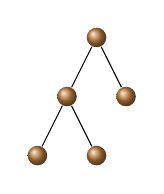
\begin{tikzpicture}[scale=.5, auto,swap, inner sep=2.5pt,]% scale=1, inner sep=5
%\useasboundingbox
%\tikz[baseline]
\tikzstyle{every node}=[ball color=brown,circle,text=white]%, minimum size=2mm]
\node at (5,0) {}
child {
	node {} 
	child {node {}}
	child {
		node {} 	
		%child {node {}} 
	}	
}
child {node {}};

;

%\begin{scope}
%\tikzstyle{every node}=[]
%\draw(2,-2) node {$\longrightarrow$};
%\end{scope}

\end{tikzpicture}
}
%%%%%%%%%%%%%%%%%%%%%%%%%%%%%%%%%%%%%%%%%%%%%%%%%%%%%%%%%
% Slide explaining NOT IMPLICIT rule
\def\Treex{

\begin{center}
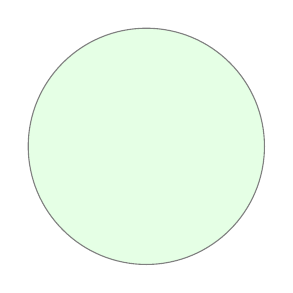
\begin{tikzpicture}[scale=.4, auto,swap, inner sep=2pt,]% scale=1, inner sep=5
%\useasboundingbox
%\tikz[baseline]

\tikzstyle{every node}=[draw=black!50,fill=green!10]
\node (ta) at (8,-2) [circle,inner sep=0pt,minimum width=3cm,minimum height=3cm] {};
%,pin=below:{\textbf{Supertree} of the antecedents} 
%pin=-120:NO Supertree of the consequent

\tikzstyle{every node}=[ball color=brown,circle,text=white]
\Tsx{8}{0}

\end{tikzpicture}

\vspace{.5cm}

This supertree of the antecedents %} supertree
is \textbf{NOT} a supertree of the consequents.% supertree 

\end{center}

}

\def\DataSet{
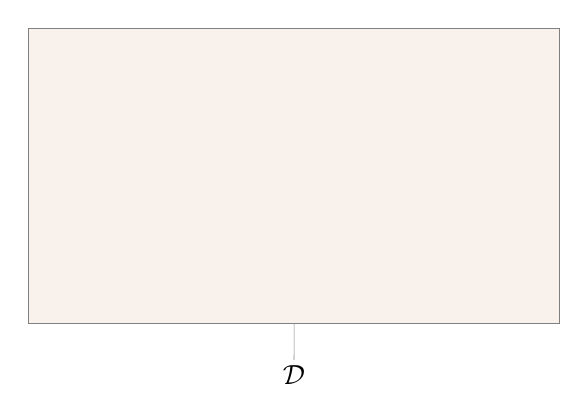
\begin{tikzpicture}[scale=.6, auto,swap, inner sep=2pt,]% scale=1, inner sep=5
%\useasboundingbox
%\tikz[baseline]

\tikzstyle{every node}=[draw=black!50,fill=brown!10]
\node (ta) at (8,-2) [rectangle,inner sep=0pt,minimum width=6.75cm,minimum height=3.75cm,pin=below:${\cal D}$] {};


\tikzstyle{every node}=[ball color=brown,circle,text=white]%, minimum size=1mm]

 \Tsa{4}{0};
 \Tsb{8}{0};
 \Tsc{12}{0};

\end{tikzpicture}
}

%%%%%%%%%%%%%%%%%%%%%%%%%%%%%%%%%%%%%%%%%%%%%%%%%%%%%%%%%
% Lattices
\def\Lattice{

\begin{tikzpicture}[scale=.6, auto,swap, inner sep=2pt,]% scale=1, inner sep=5
%\useasboundingbox
%\tikz[baseline]
\LatticeAux
\end{tikzpicture}
}

\def\LatticeAux{
\tikzstyle{every node}=[ball color=brown,circle,text=white]%, minimum size=2mm]

 \Tsa{5}{0};
 \Tsb{10}{0};
 \Tsc{15}{0};

 \Tsab{5}{-7};
 \Tsac{10}{-7};
 \Tsbc{15}{-7};

 \Tsabc{10}{-14};

\tikzstyle{every node}=[draw=black!50]%fill=blue!20,minimum size=5mm]%, minimum size=2mm]
  %\draw[style=help lines] (-1,-2) grid (6,3);

%\tikzstyle{place}=[circle,draw=blue!50,fill=blue!20,thick,
%                   inner sep=0pt,minimum size=6mm]

\node (ta) at (5,-2.5) [ellipse,inner sep=0pt,minimum width=2.25cm,minimum height=3.75cm,label=-120:$1$] {};
\node (tb) at (10,-2) [ellipse,inner sep=0pt,minimum width=3cm,minimum height=3cm,label=below:$2$] {};
\node (tc) at (15,-2.5) [ellipse,inner sep=0pt,minimum width=2.25cm,minimum height=3.75cm,label=-60:$3$] {};

\node (tab) at (5,-9) [ellipse,inner sep=0pt,minimum width=2.25cm,minimum height=3cm,label=-120:$1 2$] {};
\node (tac) at (10,-9) [ellipse,inner sep=0pt,minimum width=2.25cm,minimum height=3.75cm,label=-60:$1 3$] {};
\node (tbc) at (15,-9) [ellipse,inner sep=0pt,minimum width=2.25cm,minimum height=3cm,label=-60:$2 3$] {};

\node (tabc) at (10,-15.7) [ellipse,inner sep=0pt,minimum width=2.25cm,minimum height=3cm,label=below:$1 2 3$] {};

  %\path (0,0) node(aa) [rectangle,draw,minimum size=1cm]     {}
  %      (5,0) node(b) [circle,draw]               {}
  %      (10,-7) node(c) [rectangle,draw] {}
  %      (10,-14) node(d) [rectangle,draw] {};
  \draw[thick,blue!50] (ta) -- (tab) -- (tabc) -- (tbc) -- (tc) -- (tac) -- (tabc) -- (tab) -- (tb)
	 -- (tbc);
   \draw[thick,blue!50] (ta) -- (tac);
  %\draw[thick,red,->] (a) |- +(1,3) -| (c) |- (b);
  %\draw[thick,blue,<->] (b) .. controls +(right:2cm) and +(down:1cm) .. (d);
}




%--- Chapters -----------------------
%\pagestyle{headings}
%\pagenumbering{arabic}
\chapter*{Introduction}
\pdfbookmark[0]{Introduction}{introduction}
\thispagestyle{empty}

{\bf M}assive {\bf O}nline {\bf A}nalysis (MOA) is a %framework 
software environment for implementing algorithms and running experiments
for online learning from %continuous supplies of examples, such as 
evolving data streams.
%The data stream evaluation framework and all algorithms evaluated in this paper
%were implemented in the Java programming language extending the MOA software. %framework.

\begin{center}
\includegraphics[height=2cm]{figures/LogoMOA.jpg} \end{center}

MOA includes a collection of offline and online methods as well as tools for evaluation. 
In particular, it implements boosting, bagging, and Hoeffding Trees, all %both 
with and without Na{\"\i}ve Bayes classifiers at the leaves. 
%MOA  graphical user interface is shown in Figure~\ref{fig:moagui}.
%However, a command line interface is also available.

%\begin{figure}[t]
%\begin{center} 
%\epsfig{file=MOATL, scale=0.3}
%\end{center} 
%\caption{MOA Graphical User Interface}
%\label{fig:moagui}
%\end{figure} 

MOA is related to WEKA, the Waikato
Environment for Knowledge Analysis, which is an award-winning open-source 
workbench containing implementations of a wide range of batch machine 
learning methods. WEKA is also written in Java. The main benefits
of Java are portability, where applications can be run on any platform with
an appropriate Java virtual machine, and the strong and well-developed support 
libraries. Use of the language is widespread, and features such as the
automatic garbage collection help to reduce programmer burden and error.

This text explains the theoretical and practical foundations of the methods and streams available in MOA.
The moa and the weka are both birds native to New Zealand. The weka is a cheeky bird of similar size to a chicken. The moa was a large ostrich-like bird, an order of magnitude larger than a weka, that was hunted to extinction.

\BEGINOMIT
    One of the key data structures used in MOA is the description of an example
from a data stream. This structure borrows from WEKA, where an example is
represented by an array of double precision floating point values. This provides
freedom to store all necessary types of value \--- numeric attribute values can be
stored directly, and discrete attribute values and class labels are represented
by integer index values that are stored as floating point values in the array.
Double precision floating point values require storage space of 64 bits, or 8
bytes. This detail can have implications for memory usage. %utilization.
\ENDOMIT

\part{Introduction and Preliminaries} 
\chapter{Preliminaries}
\label{chap:introduction}

In today's information society, extraction of knowledge is becoming a very
important task for many people. We live in an age of knowledge revolution.
Peter Drucker~\cite{Drucker}, an influential management expert, writes ``From now on, the key is knowledge. The world is not becoming labor intensive, not material intensive, not energy intensive, but knowledge  intensive''.
This knowledge revolution is based in an economic 
change from adding value by producing things which is, ultimately 
limited, to adding value by creating and using knowledge which can 
grow indefinitely.

The digital universe in 2007 was estimated in~\cite{IDC} to be 281 exabytes
or 281 billion gigabytes, and by 2011, the digital universe will be 
10 times the size it was 5 years before. The amount of information created, 
or captured %, or replicated 
exceeded available storage for the first time in
2007. 

To deal with these huge amount of data in a responsible way,
green computing is becoming a necessity. {\em Green computing} 
is the study and practice of using computing resources efficiently.
A main approach to green computing is based on algorithmic efficiency.
The amount of computer resources required for any given computing function
depends on the efficiency of the algorithms used. As the cost of hardware
has declined relative to the cost of energy, the energy efficiency and 
environmental impact of computing systems and programs 
are receiving increased attention.


\section{MOA Stream Mining }

A largely untested hypothesis of modern society is that it is important to record data as it may contain valuable information. This occurs in almost all facets of life from supermarket checkouts to the movements of cows in a paddock. To support the hypothesis, engineers and scientists have produced a raft of ingenious schemes and devices from loyalty programs to RFID tags. Little thought however, has gone into how this {\em quantity} of data might be analyzed. 

{\em Machine learning}, the field for finding ways to automatically extract information from data, was once considered the solution to this problem. Historically it has concentrated on learning from small numbers of examples, because only limited amounts of data were available when the field emerged. Some very sophisticated algorithms have resulted from the research that can learn highly accurate models from limited training examples. It is commonly assumed that the entire set of training data can be stored in working memory.

More recently the need to process larger amounts of data has motivated the field of {\em data mining}. Ways are investigated to reduce the computation time and memory needed to process large but static data sets. If the data cannot fit into memory, it may be necessary to sample a smaller training set. Alternatively, algorithms may resort to temporary external storage, or only process subsets of data at a time. Commonly the goal is to create a learning process that is linear in the number of examples. The essential learning procedure is treated like a scaled up version of classic machine learning, where learning is considered a single, possibly expensive, operation---a set of training examples are processed to output a final static model.

The data mining approach may allow larger data sets to be handled, but it still does not address the problem of a {\em continuous} supply of data. Typically, a model that was previously induced cannot be updated when new information arrives. Instead, the entire training process must be repeated with the new examples included. There are situations where this limitation is undesirable and is likely to be inefficient.

The {\em data stream} paradigm has recently emerged in response to the continuous data problem. Algorithms written for data streams can naturally cope with data sizes many times greater than memory, and can extend to challenging real-time applications not previously tackled by machine learning or data mining. The core assumption of data stream processing is that training examples can be briefly inspected a single time only, that is, they arrive in a high speed stream, then must be discarded to make room for subsequent examples. The algorithm processing the stream has no control over the order of the examples seen, and must update its model incrementally as each example is inspected. An additional desirable property, the so-called {\em anytime} property, requires that the model is ready to be applied at any point between training examples.

\BEGINOMIT
The {\em Hoeffding tree} induction method, a method for producing {\em decision tree} models, represents one of the best known algorithms for classifying streams of examples. Improvements to it are the focus of this \thesis. As the method is already state-of-the-art, it is not expected that massive gains will be possible, but rather smaller incremental improvements that are beneficial nonetheless. To measure improvements to this algorithm, an evaluation framework is developed to provide useful insight about classification performance. This fosters algorithm development that results in measurably improved performance.
\ENDOMIT

Studying purely theoretical advantages of algorithms is certainly useful and enables new developments, but the demands of data streams require this to be followed up with empirical evidence of performance. Claiming that an algorithm is suitable for data stream scenarios implies that it possesses the necessary practical capabilities. Doubts remain if these claims cannot be backed by reasonable empirical evidence.

%A central argument of this \thesis is that D
Data stream classification algorithms require appropriate and complete evaluation practices. The evaluation should allow users to be sure that particular problems can be handled, to quantify improvements to algorithms, and to determine which algorithms are most suitable for their problem. \textbf{MOA} is suggested with these needs in mind.

Measuring data stream classification performance is a three dimensional problem involving processing speed, memory and accuracy. It is not possible to enforce and simultaneously measure all three at the same time so in %a new framework as
 \textbf{MOA} %this \thesis argues that 
it is necessary to fix the memory size and then record the other two. Various memory sizes can be associated with data stream application scenarios so that basic questions can be asked about expected performance of algorithms in a given application scenario. \textbf{MOA} is developed to provide useful insight about classification performance.


\section{Assumptions}

%This \thesis 
\textbf{MOA} is concerned with the problem of {\em classification}, perhaps the most commonly researched machine learning task. The goal of classification is to produce a model that can predict the class of unlabeled examples, by training on examples whose label, or {\em class}, is supplied. To clarify the problem setting being addressed, several assumptions are made about the typical learning scenario: 
\begin{enumerate}
\item The data is assumed to have a small and fixed number of columns, or {\em attributes}/{\em features}---several hundred at the most. 
\item The number of rows, or {\em examples}, is very large---millions of examples at the smaller scale. 
In fact, algorithms should have the potential to process an infinite amount of data, meaning that they will not exceed memory limits or otherwise fail no matter how many training examples are processed.
\item The data has a limited number of possible class labels, typically less than ten.
\item The amount of memory available to a learning algorithm depends on the application. The size of the training data will be considerably larger than the available memory.
\item There should be a small upper bound on the time allowed to train or classify an example. This permits algorithms to scale linearly with the number of examples, so users can process $N$ times more than an existing amount simply by waiting $N$ times longer than they already have. 
\item Stream concepts are assumed to be stationary or evolving. % in the first part, that is, the problem of {\em concept drift} is not directly addressed until the second part. 
Concept drift occurs when the underlying concept defining the target being learned begins to shift over time. %The solutions explored here could be extended to handle concept drift, but this is reserved for future work.
\end{enumerate}

The first three points emphasize that the aim is to scale with the number of examples. Data sources that are large in other dimensions, such as numbers of attributes or possible labels are not the intended problem domain. Points 4 and 5 outline what is needed from a solution. Regarding point 6, some researchers argue that addressing concept drift is one of the most crucial issues in processing data streams. %For this \thesis it is believed more important that the other requirements are met first, otherwise a solution will not be satisfactory when demands are too high regardless of whether concept drift is addressed.

\section{Requirements} 

The conventional machine learning setting, referred to in this \thesis as the {\em batch} setting, operates assuming that the training data is available as a whole set---any example can be retrieved as needed for little cost. An alternative is to treat the training data as a \emph{stream}, a potentially endless flow of data that arrives in an order that cannot be controlled.
Note that an algorithm capable of learning from a stream is, by definition, a data mining algorithm.

Placing classification in a data stream setting offers several advantages. Not only is the limiting assumption of early machine learning techniques addressed, but other applications even more demanding than mining of large databases can be attempted. An example of such an application is the monitoring of high-speed network traffic, where the unending flow of data is too overwhelming to consider storing and revisiting.

A classification algorithm must meet several requirements in order to work with the assumptions and be suitable for learning from data streams. The requirements, numbered 1 through 4, are detailed below.


\subsection*{Requirement 1: Process an example at a time, and inspect it only once (at most)}

The key characteristic of a data stream is that data `flows' by one example after another. There is no allowance for \emph{random access} of the data being supplied. Each example must be accepted as it arrives in the order that it arrives. Once inspected or ignored, an example is discarded with no ability to retrieve it again.

Although this requirement exists on the input to an algorithm, there is no rule preventing an algorithm from remembering examples internally in the short term. An example of this may be the algorithm storing up a \emph{batch} of examples for use by a conventional learning scheme. While the algorithm is free to operate in this manner, it will have to discard stored examples at some point if it is to adhere to requirement 2.

The inspect-once rule may only be relaxed in cases where it is practical to re-send the entire stream, equivalent to multiple scans over a database. In this case an algorithm may be given a chance during subsequent passes to refine the model it has learned. However, an algorithm that requires any more than a single pass to operate is not flexible enough for universal applicability to data streams.

\subsection*{Requirement 2: Use a limited amount of memory}

The main motivation for employing the data stream model is that it allows processing of data that is many times larger than available working memory. The danger with processing such large amounts of data is that memory is easily exhausted if there is no intentional limit set on its use.

Memory used by an algorithm can be divided into two categories: memory used to store running statistics, and memory used to store the current model. For the most memory-efficient algorithm they will be one and the same, that is, the running statistics directly constitute the model used for prediction.

This memory restriction is a physical restriction that can only be relaxed if external storage is used, temporary files for example. Any such work-around needs to be done with consideration of requirement 3.

\subsection*{Requirement 3: Work in a limited amount of time}

For an algorithm to scale comfortably to any number of examples, its runtime complexity must be linear in the number of examples. This can be achieved in the data stream setting if there is a constant, preferably small, upper bound on the amount of processing per example.

Furthermore, if an algorithm is to be capable of working in \emph{real-time}, it must process the examples as fast if not faster than they arrive. Failure to do so inevitably means loss of data.

Absolute timing is not as critical in less demanding applications, such as when the algorithm is being used to classify a large but persistent data source. However, the slower the algorithm is, the less value it will be for users who require results within a reasonable amount of time.

\subsection*{Requirement 4: Be ready to predict at any point}

An ideal algorithm should be capable of producing the best model it can from the data it has observed after seeing any number of examples. In practice it is likely that there will be periods where the model stays constant, such as when a batch based algorithm is storing up the next batch.

The process of generating the model should be as efficient as possible, the best case being that no translation is necessary. That is, the final model is directly manipulated in memory by the algorithm as it processes examples, rather than having to recompute the model based on running statistics. 

\subsection*{The data stream classification cycle}

\begin{figure}
\centering
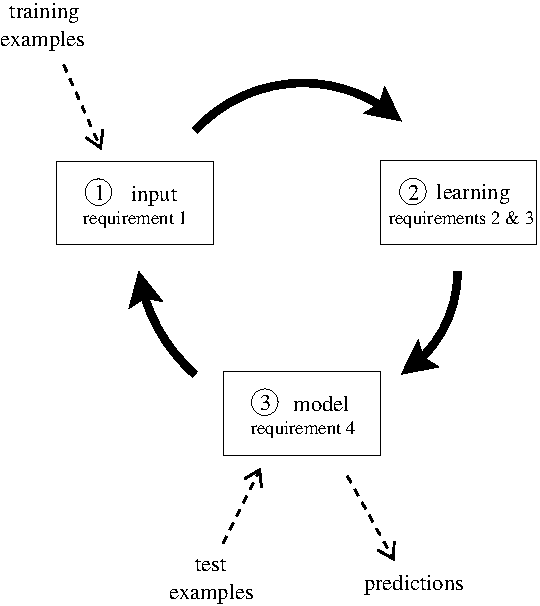
\includegraphics{figures/ds_cycle}
\caption{The data stream classification cycle.}
\label{fig:ds_cycle}
\end{figure}

Figure~\ref{fig:ds_cycle} illustrates the typical use of a data stream classification algorithm, and how the requirements fit in. The general model of data stream classification follows these three steps in a repeating cycle:

\begin{enumerate}

\item The algorithm is passed the next available example from the stream (requirement 1).

\item The algorithm processes the example, updating its data structures. It does so without exceeding the memory bounds set on it (requirement 2), and as quickly as possible (requirement 3).

\item The algorithm is ready to accept the next example. On request it is able to supply a model that can be used to predict the class of unseen examples (requirement 4).

\end{enumerate}

\section{Mining Strategies} 

The task of modifying machine learning algorithms to handle large data sets is known as {\em scaling up}~\cite{ml_scaleup}.
Analogous to approaches used in data mining, there are two general strategies for taking machine learning concepts and applying them to data streams. The \emph{wrapper} approach aims at maximum reuse of existing schemes, whereas \emph{adaptation} looks for new methods tailored to the data stream setting.

Using a wrapper approach means that examples must in some way be collected into a batch so that a traditional batch learner can be used to induce a model. The models must then be chosen and combined in some way to form predictions. The difficulties of this approach include determining appropriate training set sizes, and also that training times will be out of the control of a wrapper algorithm, other than the indirect influence of adjusting the training set size. When wrapping around complex batch learners, training sets that are too large could stall the learning process and prevent the stream from being processed at an acceptable speed. Training sets that are too small will induce models that are poor at generalizing to new examples. Memory management of a wrapper scheme can only be conducted on a per-model basis, where memory can be freed by forgetting some of the models that were previously induced. Examples of wrapper approaches from the literature include Wang et al.~\cite{cdensemble}, Street and Kim~\cite{sea} and Chu and Zaniolo~\cite{fastlightboost}. 

Purposefully adapted algorithms designed specifically for data stream problems offer several advantages over wrapper schemes. They can exert greater control over processing times per example, and can conduct memory management at a finer-grained level.
Common varieties of machine learning approaches to classification fall into several general classes. These classes of method are discussed below, along with their potential for adaptation to data streams:


\begin{description}
\item[decision trees] This class of method is the main focus of the \thesis. Chapter~\ref{chap:hoeffdingtrees} studies a successful adaptation of decision trees to data streams~\cite{vfdt} and outlines the motivation for this choice.
\item[rules] Rules are somewhat similar to decision trees, as a decision tree can be decomposed into a set of rules, although the structure of a rule set can be more flexible than the hierarchy of a tree. Rules have an advantage that each rule is a disjoint component of the model that can be evaluated in isolation and removed from the model without major disruption, compared to the cost of restructuring decision trees. However, rules may be less efficient to process than decision trees, which can guarantee a single decision path per example. Ferrer-Troyano et al.~\cite{scallop, dsrules} have developed methods for inducing rule sets directly from streams.
\item[lazy/nearest neighbour] This class of method is described as {\em lazy} because in the batch learning setting no work is done during training, but all of the effort in classifying examples is delayed until predictions are required. The typical {\em nearest neighbour} approach will look for examples in the training set that are most similar to the example being classified, as the class labels of these examples are expected to be a reasonable indicator of the unknown class. The challenge with adapting these methods to the data stream setting is that training can not afford to be lazy, because it is not possible to store the entire training set. Instead the examples that are remembered must be managed so that they fit into limited memory. An intuitive solution to this problem involves finding a way to merge new examples with the closest ones already in memory, the main question being what merging process will perform best. Another issue is that searching for the nearest neighbours is costly. This cost may be reduced by using efficient data structures designed to reduce search times. Nearest neighbour based methods are a popular research topic for data stream classification. Examples of systems include~\cite{anncad, lwclass, ds-knn, ds-instancebased}.
\item[support vector machines/neural networks] Both of these methods are related and of similar power, although {\em support vector machines}~\cite{svm} are induced via an alternate training method and are a hot research topic due to their flexibility in allowing various {\em kernels} to offer tailored solutions.
Memory management for support vector machines could be based on limiting the number of support vectors being induced. Incremental training of support vector machines has been explored previously, for example~\cite{incrsvm}.
Neural networks are relatively straightforward to train on a data stream. A real world application using neural networks is given by Gama and Rodrigues~\cite{gama_ann}. The typical procedure assumes a fixed network, so there is no memory management problem. It is straightforward to use the typical {\em backpropagation} training method on a stream of examples, rather than repeatedly scanning a fixed training set as required in the batch setting.
\item[Bayesian methods] These methods are based around {\em Bayes' theorem} and compute probabilities in order to perform {\em Bayesian inference}. The simplest Bayesian
method, Naive Bayes, is described in Section~\ref{sec:nbleaf}, and is a special case of algorithm that needs no adaptation to data streams. This is because it is straightforward to train incrementally and does not add structure to the model, so that memory usage is small and bounded. A single Naive Bayes model will generally not be as accurate as more complex models. The more general case of {\em Bayesian networks} is also suited to the data stream setting, at least when the structure of the network is known. Learning a suitable structure for the network is a more difficult problem. Hulten and Domingos~\cite{mineabitrarydb} describe a method of learning Bayesian networks from data streams using Hoeffding bounds. Bouckaert~\cite{remcobayesstream} also presents a solution.
\item[meta/ensemble methods] These methods wrap around other existing methods, typically building up an {\em ensemble} of models. Examples of this include~\cite{ozabagboost, anncad}. This is the other major class of algorithm studied in-depth by this \thesis, beginning in Chapter~\ref{chap:improvebackground}.
\end{description}

Gaber et al.~\cite{dssurvey} survey the field of data stream classification algorithms and list those that they believe are major contributions. Most of these have already been covered: Domingos and Hulten's {\em VFDT}~\cite{vfdt}, the decision tree algorithm studied in-depth by this \thesis; {\em ensemble-based classification} by Wang et al.~\cite{cdensemble} that has been mentioned as a wrapper approach; {\em SCALLOP}, a rule-based learner that is the earlier work of Ferrer-Troyano et al.~\cite{scallop}; {\em ANNCAD}, which is a nearest neighbour method developed by Law and Zaniolo~\cite{anncad} that operates using {\em Haar wavelet} transformation of data and small classifier ensembles; and {\em LWClass} proposed by Gaber et al.~\cite{lwclass}, another nearest neighbour based technique, that actively adapts to fluctuating time and space demands by varying a distance threshold. The other methods in their survey that have not yet been mentioned include {\em on demand classification}. This method by Aggarwal et al.~\cite{ondemand} performs dynamic collection of training examples into supervised {\em micro-clusters}. From these clusters, a nearest neighbour type classification is performed, where the goal is to quickly adapt to concept drift. The final method included in the survey is known as an {\em online information network} ({\em OLIN}) proposed by Last~\cite{olin}. This method has a strong focus on concept drift, and uses a {\em fuzzy} technique to construct a model similar to decision trees, where the frequency of model building and training window size is adjusted to reduce error as concepts evolve.

\BEGINOMIT
Of the broad classes of algorithm, there are no existing benchmarks to determine which class is superior to any other at classifying data streams. Decision trees were chosen because they are a classic area of research, and there is existing evidence to suggest that they are an effective method for data stream classification.


\section{Thesis Structure}

The chapters that follow build the \thesis in logical sequence:

Chapter~\ref{chap:experimentalsetting} reviews the common methodologies in practice for evaluating data stream algorithms. After considering the desirable attributes of a comprehensive evaluation strategy a final framework is proposed. The framework includes simulation of three environments by varying memory demands, and a set of synthetic data generators in preparation for evaluation of  learning algorithms in the \thesis.

Chapter~\ref{chap:hoeffdingtrees} introduces the basic decision tree learning algorithm that operates on data streams by relying on Hoeffding bounds to decide when sufficient information has been seen to justify tree expansion. Many aspects of the basic algorithm are explored.

Chapter~\ref{chap:numericatts} sets out to resolve the issue of how Hoeffding trees should handle continuous numeric attributes. Potential approaches are surveyed, and then candidates are tested using the evaluation framework from Chapter~\ref{chap:experimentalsetting} in an experiment to determine which strategy performs best.

Chapter~\ref{chap:predstrat} conducts a study of prediction methods, using the evaluation framework from Chapter~\ref{chap:experimentalsetting} to produce empirical evidence in support of a newly suggested method. This hybrid approach adaptively combines the strengths of two previous methods.

Chapter~\ref{chap:improvebackground} surveys common methods for improving accuracy in the batch setting via ensembles of models. Possibilities for transferring these methods to data streams are explored, along with the theoretical implications of combining increasing numbers of models when memory is limited. Algorithms are elaborated, including a novel method of inducing {\em option trees}---a generalized representation of decision trees offering the benefits of ensembles in a single and potentially more memory-efficient structure.

Chapter~\ref{chap:improvecompare} experimentally compares the main algorithms suggested in Chapter~\ref{chap:improvebackground} using the evaluation framework from Chapter~\ref{chap:experimentalsetting}. Some of the results on data stream problems are surprising, and some do not entirely match the expectations arising from generalizations in the batch setting, so a deeper analysis and discussion looks more closely at the issues.

Chapter~\ref{chap:conclusions} summarizes the findings and lists the contributions made. It concludes with a discussion of potential for future work.
\ENDOMIT

%\section{Evolving Stream Mining Strategies}

 Dealing with time-changing data requires %in turn 
strategies for detecting and quantifying change, forgetting stale examples, 
and for model revision. Fairly generic strategies exist for detecting
change and deciding when examples are no longer relevant. %Model revision
%strategies, on the other hand, are in most cases method-specific.
\BEGINOMIT
Most strategies for dealing with time change contain hardwired constants, 
or else require input parameters, concerning the expected speed or frequency 
of the change; some examples are {\em a priori} definitions of sliding window
lengths, values of decay or forgetting parameters, explicit bounds on maximum drift, etc. 
%\BEGINOMIT
These choices represent preconceptions 
on how fast or how often the data are going to evolve and, of course, they 
may be completely wrong. Even more, no fixed 
choice may be right, since the stream may experience any combination 
of abrupt changes, gradual ones, and long stationary periods. 
More in general, an approach based on fixed parameters will be caught in the following tradeoff: 
the user would like to use values of parameters that give more accurate statistics 
(hence, more precision) during periods of stability, but at the same time use the opposite values of
 parameters to %be able to 
quickly react to changes, when they occur. 
%\ENDOMIT

Many ad-hoc methods have been used to deal with drift, often tied to particular algorithms. 
%In Section~\ref{Sframework} %
\ENDOMIT
\BEGINOMIT
In this chapter we propose a more general approach based on using two primitive design 
elements: change detectors and estimators. 
The idea is to 
encapsulate all the statistical calculations having to do with detecting change and keeping
updated statistics from a stream an abstract data type that can then be used to replace, 
in a black-box way, the counters and accumulators that typically all machine learning
and data mining algorithms use to make their decisions, including when change has occurred. 

We believe that, compared to any previous approaches, our approach better isolates different
concerns when designing new data mining algorithms, therefore reducing design time,
increasing modularity, and facilitating analysis. Furthermore, since we crisply identify
the nuclear problem in dealing with drift, and use a well-optimized algorithmic solution to tackle it,
the resulting algorithms are more accurate, adaptive, and time- and memory-efficient than other
ad-hoc approaches. % starting from scratch. 
%We have given evidence for this superiority in \cite{bif-gav,Kbif-gav,KDD08}
%and we demonstrate this idea again here.

\subsection{Theoretical approaches}%Learning time-varying concepts}

The task of learning drifting or time-varying concepts has also been studied
 in computational learning theory. Learning a changing concept is infeasible,
 if no restrictions are imposed on the type of admissible concept changes,  
but drifting concepts are provably efficiently learnable (at least for certain 
concept classes), if the rate or the extent of drift is limited in particular ways. 

Helmbold and Long \cite{helmbold94tracking} assume a possibly permanent but slow concept 
drift and define the extent of drift as the probability that two subsequent 
concepts disagree on a randomly drawn example. Their results include an 
upper bound for the extend of drift maximally tolerable by any learner and 
algorithms that can learn concepts that do not drift more than a certain 
constant extent of drift. Furthermore they show that it is sufficient for a 
learner to see a fixed number of the most recent examples. Hence a window 
of a certain minimal fixed size allows to learn concepts for which the extent 
of drift is appropriately limited. 
While Helmbold and Long restrict the extend of drift, Kuh, Petsche, and 
Rivest~\cite{kuh} determine a maximal rate of drift that is acceptable by any learner, 
i. e. a maximally acceptable frequency of concept changes, which implies a 
lower bound for the size of a fixed window for a time-varying concept to be 
learnable, which is similar to the lower bound of Helmbold and Long. 

\ENDOMIT

%\section{Change Detection and Value Estimation}
%\label{SChange}
\section{Change Detection Strategies} 

The following different modes of change have been identified in the literature~\cite{tsymbal-problem,stanley03learning,WidmerKubat}:

\begin{itemize}
\item concept change
\begin{itemize}
\item concept drift
\item concept shift
\end{itemize}
\item distribution or sampling change
\end{itemize}

\textit{Concept} refers to the target variable, which the model is trying to predict.
\textit{Concept change} is the change of the underlying concept over time.
Concept drift describes a gradual change of the concept
and concept shift happens when a change between two concepts is more abrupt. 

\textit{Distribution change}, also known as sampling
change or shift or virtual concept drift , refers to the change in the data distribution.
Even if the concept remains the same, the change may often lead to revising the
current model as the model's error rate may no longer be acceptable with the
new data distribution.

Some authors, as Stanley~\cite{stanley03learning}, have suggested that from the practical point of view, it is not
essential to differentiate between concept change and sampling change since the
current model needs to be changed in both cases.
%We agree to some extent, and our methods will not be targeted to one particular type of change.
%Both cases of concept drift and concept shift abound in the
%real world. Since they have different characteristics, they may require different
%optimal prediction strategies.

%%%%%%%%%%%%%%%%%%%%%%%%%%%%%%%%%%%%%%%%%%%%%%%%%%%%%%%
%\subsection{Change Detection}

Change detection is not an easy task, since a fundamental
limitation exists~\cite{Gustaffson:2000}: the design of a change detector
is a compromise between detecting true changes and avoiding false
alarms. 
See~\cite{Gustaffson:2000,Baseville93} for more detailed surveys of change detection methods.

\subsubsection{The CUSUM Test}
\label{Sscusum}

The cumulative sum (CUSUM algorithm), %which was
 first proposed in \cite{Page54}, 
is a change detection algorithm that gives an alarm when the mean of the input data is significantly 
different from zero. The CUSUM input $\epsilon_t$ can be any filter residual, for instance 
the prediction error from a Kalman filter.

The CUSUM test is as follows:
$$g_0=0$$
$$g_t=\mbox{max }(0,g_{t-1}+ \epsilon_t -\upsilon)$$
$$\mbox{if } g_t>h \mbox{ then alarm and } g_t=0$$
%
The CUSUM test is memoryless, and its accuracy depends on the choice of parameters $\upsilon$ and $h$.

\subsubsection{The Geometric Moving Average Test}
\label{Ssgma}
The CUSUM test is a stopping rule. Other stopping rules exist. For example, the Geometric Moving Average (GMA) test,
first proposed in~\cite{Roberts}, is the following
$$g_0=0$$
$$g_t= \lambda g_{t-1}+ ( 1- \lambda) \epsilon_t$$
$$\mbox{if } g_t>h \mbox{ then alarm and } g_t=0$$
The forgetting factor $\lambda$ is used to give more or less weight to the last data arrived.
The treshold $h$ is used to tune the sensitivity and false alarm rate %performance 
of the detector.


\subsubsection{Statistical Tests}
\label{Ssstatic}

CUSUM and GMA are methods for dealing with numeric sequences. For more complex populations,
we need to use other methods.
There exist some statistical tests that may be used to detect change.
A statistical test is a procedure for deciding whether a hypothesis 
about a quantitative feature of a population is true or false. We test 
an hypothesis of this sort by drawing a random sample from the population
 in question and calculating an appropriate statistic on its items. 
If, in doing so, we obtain a value of the statistic that would occur
 rarely when the hypothesis is true, we would have reason to reject the hypothesis. 

To detect change, we need to compare two sources of data, and decide if
the hypothesis $H_0$ that they come from the same distribution is true. 
Let's suppose we have two estimates, $\hmu_0$ and $\hmu_1$ with variances
$\sigma_0^2$ and $\sigma_1^2$. If there is no change in the data, 
these estimates will be consistent. Otherwise, a hypothesis test will
reject $H_0$ and a change is detected. There are several ways to construct
such a hypothesis test. The simplest one is to study the difference

$$ \hmu_0 - \hmu_1 \in N(0, \sigma_0^2+ \sigma_1^2), \mbox{ under } H_0$$

or, to make a $\chi^ 2$ test

$$ \frac{(\hmu_0 - \hmu_1)^ 2}{\sigma_0^2+ \sigma_1^2} \in \chi^ 2(1), \mbox{ under } H_0$$

from which a standard hypothesis test can be formulated. 

For example, suppose we want to design a change detector using a statistical test
with a probability of false alarm of $5\%$, that is,

$$\Pr \left( \frac{|\hmu_0 - \hmu_1|}{\sqrt{\sigma_0^2+ \sigma_1^2}} > h \right) = 0.05$$

A table of the Gaussian distribution shows that $P( X< 1.96) = 0.975$, so the test becomes

$$\frac{(\hmu_0 - \hmu_1)^ 2}{{\sigma_0^2+ \sigma_1^2}} > 1.96$$
Note that this test uses the normality hypothesis. In Chapter~\ref{ch:adwin} we will propose a similar test with
theoretical guarantees. However, 
we could have used this test on the methods of Chapter~\ref{ch:adwin}.

The Kolmogorov-Smirnov test~\cite{Kanji} is another statistical test used to compare two populations.
Given samples %of size $n_1$ and $n_2$ 
from two populations, the cumulative distribution functions %$S_{n_1}(x)$ and $S_{n_2}(y)$ 
can be determined and plotted. Hence the maximum value of the difference between the plots can be found and compared with a critical value. If the
observed value exceeds the critical value, %the null hypothesis that the two population distributions are identical 
$H_0$ is rejected and a change is detected. It is not obvious how to implement the  Kolmogorov-Smirnov test dealing with data streams. Kifer et al.~\cite{kifer-detecting} propose a KS-structure to implement Kolmogorov-Smirnov and similar tests, on the data stream setting.

\subsubsection{Drift Detection Method}
\label{SsDDM}

The drift detection method (DDM) proposed by Gama et al.  \cite{Gama} controls the number of errors produced by
the learning model during prediction. %It uses a binomial distribution that 
%gives the general form of the probability for the random variable that represents the
It compares the statistics of two windows: the first one contains all the data, and the second one contains only the data from the beginning until the number of errors increases. This method does not store these windows in memory. It keeps only statistics and a window of recent data.% since a warning signal is detected.

The number of errors in a sample of $n$ examples is modelized by a binomial distribution. For each point $i$ in the sequence
that is being sampled, the error rate is the probability of misclassifying ($p_i$),
with standard deviation given by $s_i = \sqrt{p_i(1 - p_i)/i}$. It assumes (as can be argued e.g. in the
PAC learning model \cite{Mitchell}) that the error rate of the learning algorithm ($p_i$) will
decrease while the number of examples increases if the distribution of the examples is stationary. A significant increase in the error of the algorithm, suggests
that the class distribution is changing and, hence, the actual decision model is
supposed to be inappropriate. Thus, it stores the values of $p_i$ and $s_i$ when
$p_i+s_i$ reaches its minimum value during the process (obtaining $p_{pmin}$ and $s_{min}$),
and when the following conditions triggers:
\begin{itemize}
\item $p_i + s_i \geq p_{min} + 2 \cdot s_{min}$ for the warning level. Beyond this level, the examples are stored in anticipation of a possible change of context.

\item $p_i + s_i \geq p_{min} + 3 \cdot s_{min}$ for the drift level. Beyond this level the concept drift is supposed to be true, the model induced by the learning method is reset and a new model is learnt using the examples stored since the warning level triggered. The values for $p_{min}$ and $s_{min}$ are reset too.

\end{itemize}

This approach has a good behaviour of detecting abrupt changes and gradual
changes when the gradual change is not very slow, but it has difficulties when
the change is slowly gradual. In that case, the examples will be stored for long
time, the drift level can take too much time to trigger and the example memory
can be exceeded.

Baena-Garc\'{\i}a et al. proposed a new method EDDM in order to improve DDM. 
EDDM~\cite{EDDM} is shown to be better
than DDM for some data sets and worse for others. It is based on the 
estimated distribution of the distances between classification errors.
The window resize procedure is governed by the same heuristics.


%\subsection{Other change detection methods}
\label{Ssochange}


%\subsection{Estimation}
\subsubsection{Exponential Weighted Moving Average}
\label{Ssewma}

%The Estimator component
An Estimator is an algorithm that estimates the desired statistics on the input data, which
may change over time. %The algorithm may or may not use the data contained in the Memory. 
The simplest Estimator algorithm for the expected is the {\em linear estimator,}
which simply returns the average of the data items contained in the Memory. 
Other examples of run-time efficient estimators are 
Auto-Regressive, Auto Regressive Moving Average, and Kalman filters. 

An exponentially weighted moving average (EWMA) estimator is 
an algorithm that updates the estimation of a variable by combining the most 
recent measurement of the variable with the EWMA of all previous measurements:
$$ X_t=\alpha z_t + (1 -\alpha) X_{t-1} = X_{t-1} + \alpha (z_t -X_{t-1}) $$ 
where $X_t$ is the moving average, $z_t$ is the latest measurement, and $\alpha$
 is the weight given to the latest measurement (between 0 and 1). 
The idea is to produce an estimate that gives more weight to recent measurements, 
on the assumption that recent measurements are more likely to be relevant. 
Choosing an adequate $\alpha$ is a difficult problem, and it is not trivial.





 %\cleardoublepage{}
\chapter{MOA Experimental Setting}
\label{chap:experimentalsetting} 

This chapter establishes the settings under which stream mining experiments may be conducted, presenting the framework \textbf{MOA} %necessary
 to place various learning algorithms under test.
This experimental methodology %adopted by this \thesis 
is motivated by the requirements of the end user and their desired application.

\begin{figure}[ht]
\begin{center}
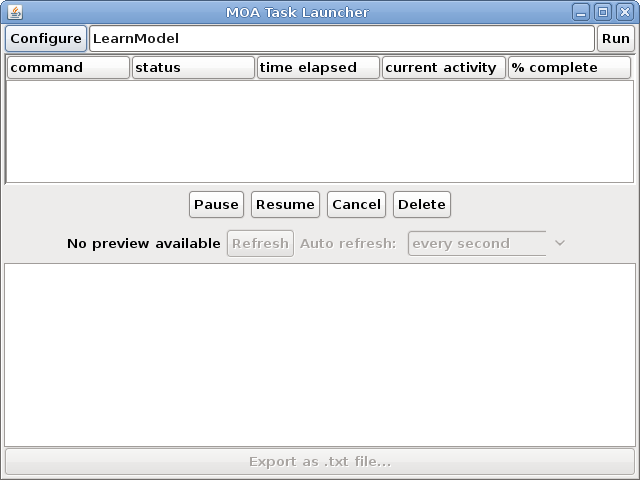
\includegraphics[height=6cm]{figures/MOATask.png}\end{center}
\caption{Graphical user interface of MOA}
\end{figure}

A user wanting to classify examples in a stream of data will have a set of requirements. They will have a certain volume of data, composed of a number of features per example, and a rate at which examples arrive. They will have the computing hardware on which the training of the model and the classification of new examples is to occur.
Users will naturally seek the most accurate predictions possible on the hardware provided. They are, however, more likely to accept a solution that sacrifices accuracy in order to function, than no solution at all. Within reason the user's requirements may be relaxed, such as reducing the training features or upgrading the hardware, but there comes a point at which doing so would be unsatisfactory.

The behaviour of a data stream learning algorithm has three dimensions of interest---the amount of space (computer memory) required, the time required to learn from training examples and to predict labels for new examples, and the error of the predictions.
When the user's requirements cannot be relaxed any further, the last remaining element that can be tuned to meet the demands of the problem is the {\em effectiveness} of the learning algorithm---the ability of the algorithm to output minimum error in limited time and space.

The error of an algorithm is the dimension that people would like to control the most, but it is the least controllable. The biggest factors influencing error are the {\em representational power} of the algorithm, how capable the model is at capturing the true underlying concept in the stream, and its {\em generalization power}, how successfully it can ignore noise and isolate useful patterns in the data.

Adjusting the time and space used by an algorithm can influence error. Time and space are interdependent. By storing more pre-computed information, such as look up tables, an algorithm can run faster at the expense of space. An algorithm can also run faster by processing less information, either by stopping early or storing less, thus having less data to process. The more time an algorithm has to process, or the more information that is processed, the more likely it is that error can be reduced.

The time and space requirements of an algorithm can be controlled by design. The algorithm can be optimised to reduce memory footprint and runtime. More directly, an algorithm can be made aware of the resources it is using and dynamically adjust. For example, an algorithm can take a memory limit as a parameter, and take steps to obey the limit. Similarly, it could be made aware of the time it is taking, and scale computation back to reach a time goal.

The easy way to limit either time or space is to stop once the limit is reached, and resort to the best available output at that point. For a time limit, continuing to process will require the user to wait longer, a compromise that may be acceptable in some situations. For a space limit, the only way to continue processing is to have the algorithm specifically designed to discard some of its information, hopefully information that is least important.
Additionally, time is highly dependent on physical processor implementation, whereas memory limits are universal.
The space requirement is a hard overriding limit that is ultimately dictated by the hardware available. An algorithm that requests more memory than is available will cease to function, a consequence that is much more serious than either taking longer, or losing accuracy, or both.

It follows that the space dimension should be fixed in order to evaluate algorithmic performance. 
Accordingly, to evaluate the ability of an algorithm to meet user requirements, a memory limit is set, and the resulting time and error performance of the algorithm is measured on a data stream.
Different memory limits have been chosen to gain insight into general performance of algorithmic variations by covering a range of plausible situations.

Several elements are covered in order to establish the evaluation framework used in this \thesisc. Evaluation methods already established in the field are surveyed in Section~\ref{sec:preveval}. Possible procedures are compared in~\ref{sec:evalcomp} and the final evaluation framework is described in Section~\ref{sec:framework}. The memory limits used for testing are motivated in Section~\ref{sec:environments}, and Section~\ref{sec:datasets} describes the data streams used for testing. Finally, Section~\ref{sec:genspeed} analyzes the speeds and sizes of the data streams involved. The particular algorithms under examination are the focus of the remainder of the \thesisc. 

\section{Previous Evaluation Practices}
\label{sec:preveval}

This section assumes that the critical variable being measured by evaluation processes is the {\em accuracy} of a learning algorithm. Accuracy, or equivalently its converse, {\em error}, may not be the only concern, but it is usually the most pertinent one. Accuracy is typically measured as the percentage of correct classifications that a model makes on a given set of data, the most accurate learning algorithm is the one that makes the fewest mistakes when predicting labels of examples. With classification problems, achieving the highest possible accuracy is the most immediate and obvious goal.
Having a reliable estimate of accuracy enables comparison of different methods, so that the best available method for a given problem can be determined.

It is very {\em optimistic} to measure the accuracy achievable by a learner on the same data that was used to train it, because even if a model achieves perfect accuracy on its training data this may not reflect the accuracy that can be expected on unseen data---its {\em generalization} accuracy.
For the evaluation of a learning algorithm to measure practical usefulness, the algorithm's ability to generalize to previously unseen examples must be tested. A model is said to {\em overfit} the data if it tries too hard to explain the training data, which is typically noisy, so performs poorly when predicting the class label of examples it has not seen before. One of the greatest challenges of machine learning is finding algorithms that can avoid the problem of overfitting.

\subsection{Batch Setting}

Previous work on the problem of evaluating batch learning has concentrated on making the best use of a limited supply of data.
When the number of examples available to describe a problem is in the order of hundreds or even less then reasons for this concern are obvious. When data is scarce, ideally all data that is available should be used to train the model, but this will leave no remaining examples for testing. The following methods discussed are those that have in the past been considered most suitable for evaluating batch machine learning algorithms, and are studied in more detail by Kohavi~\cite{cvstudy}.

% holdout

The {\em holdout} method divides the available data into two subsets that are mutually exclusive. One of the sets is used for training, the {\em training} set, and the remaining examples are used for testing, the {\em test} or {\em holdout} set. Keeping these sets separate ensures that generalization performance is being measured. Common size ratios of the two sets used in practice are 1/2 training and 1/2 test, or 2/3 training and 1/3 test. Because the learner is not provided the full amount of data for training, assuming that it will improve given more data, the performance estimate will be pessimistic. The main criticism of the holdout method in the batch setting is that the data is not used efficiently, as many examples may never be used to train the algorithm. The accuracy estimated from a single holdout can vary greatly depending on how the sets are divided. To mitigate this effect, the process of {\em random subsampling} will perform multiple runs of the holdout procedure, each with a different random division of the data, and average the results. Doing so also enables measurement of the accuracy estimate's variance. Unfortunately this procedure violates the assumption that the training and test set are independent---classes over-represented in one set will be under-represented in the other, which can skew the results. 

% cross-validation

In contrast to the holdout method, {\em cross-validation} maximizes the use of examples for both training and testing. In $k$-fold cross-validation the data is randomly divided into $k$ independent and approximately equal-sized {\em folds}. The evaluation process repeats $k$ times, each time a different fold acts as the holdout set while the remaining folds are combined and used for training. The final accuracy estimate is obtained by dividing the total number of correct classifications by the total number of examples. In this procedure each available example is used $k-1$ times for training and exactly once for testing. This method is still susceptible to imbalanced class distribution between folds. Attempting to reduce this problem, {\em stratified cross-validation} distributes the labels evenly across the folds to approximately reflect the label distribution of the entire data. Repeated cross-validation repeats the cross-validation procedure several times, each with a different random partitioning of the folds, allowing the variance of the accuracy estimate to be measured.

% leave-one-out

The {\em leave-one-out} evaluation procedure is a special case of cross-validation where every fold contains a single example. This means with a data set of $n$ examples that $n$-fold cross validation is performed, such that $n$ models are induced, each of which is tested on the single example that was held out. In special situations where learners can quickly be made to `forget' a single training example this process can be performed efficiently, otherwise in most cases this procedure is expensive to perform. The leave-one-out procedure is attractive because it is completely deterministic and not subject to random effects in dividing folds. However, stratification is not possible and it is easy to construct examples where leave-one-out fails in its intended task of measuring generalization accuracy. Consider what happens when evaluating using completely random data with two classes and an equal number of examples per class---the best an algorithm can do is predict the majority class, which will always be incorrect on the example held out, resulting in an accuracy of 0\%, even though the expected estimate should be 50\%.

% stratification

% bootstrap

An alternative evaluation method is the {\em bootstrap} method introduced by Efron~\cite{bootstrap}. This method creates a {\em bootstrap sample} of a data set by sampling with replacement a training data set of the same size as the original. Under the process of sampling with replacement the probability that a particular example will be chosen is approximately 0.632, so the method is commonly known as the 0.632 bootstrap. All examples not present in the training set are used for testing, which will contain on average about 36.8\% of the examples. The method compensates for lack of unique training examples by combining accuracies measured on both training and test data to reach a final estimate:
\begin{equation} \label{eq:bstrap}
accuracy_{bootstrap} = 0.632 \times accuracy_{test} + 0.368 \times accuracy_{train}
\end{equation}
As with the other methods, repeated random runs can be averaged to increase the reliability of the estimate. This method works well for very small data sets but suffers from problems that can be illustrated by the same situation that causes problems with leave-one-out, a completely random two-class data set---Kohavi~\cite{cvstudy} argues that although the true accuracy of any model can only be 50\%, a classifier that memorizes the training data can achieve $accuracy_{train}$ of 100\%, resulting in $accuracy_{bootstrap} = 0.632 \times 50\% + 0.368 \times 100\% = 68.4\%$. This estimate is more optimistic than the expected result of 50\%.

% standard use

Having considered the various issues with evaluating performance in the batch setting, the machine learning community has settled on stratified ten-fold cross-validation as the standard evaluation procedure, as recommended by Kohavi~\cite{cvstudy}. For increased reliability, ten repetitions of ten-fold cross-validation are commonly used. Bouckaert~\cite{remco_choose} warns that results based on this standard should still be treated with caution.

\subsection{Data Stream Setting}
\label{sec:dsevalsurvey}

The data stream setting has different requirements from the batch setting. In terms of evaluation, batch learning's focus on reusing data to get the most out of a limited supply is not a concern as data is assumed to be abundant. With plenty of data, generalization accuracy can be measured via the holdout method without the same drawbacks that prompted researchers in the batch setting to pursue other alternatives. The essential difference is that a large set of examples for precise accuracy measurement can be set aside for testing purposes without starving the learning algorithms of training examples.

Instead of maximizing data use, the focus shifts to trends over time---in the batch setting a single static model is the final outcome of training, whereas in the stream setting the model evolves over time and can be employed at different stages of growth.
In batch learning the problem of limited data is overcome by analyzing and averaging multiple models produced with different random arrangements of training and test data. In the stream setting the problem of (effectively) unlimited data poses different challenges. One solution involves taking  snapshots at different times during the induction of a model to see how much the model improves with further training. 

Data stream classification is a relatively new field, and as such evaluation practices are not nearly as well researched and established as they are in the batch setting. Although there are many recent computer science papers about data streams, only a small subset actually deal with the stream classification problem as defined in this \thesisc. A survey of the literature in this field was done to sample typical evaluation practices. Eight papers were found representing examples of work most closely related to this study. The papers are Domingos and Hulten~\cite{vfdt}, Gama et al.~\cite{vfdtc}, Gama et al.~\cite{ufft}, Jin and Agrawal~\cite{nip}, Oza and Russell~\cite{ozaexp}, Street and Kim~\cite{sea}, Fern and Givan~\cite{branchpred}, and Chu and Zaniolo~\cite{fastlightboost}. Important properties of these papers are summarized in Tables~\ref{tab:evalsurvey1} and~\ref{tab:evalsurvey2}.

\begin{table}
\caption{Paper survey part 1---Evaluation methods and data sources.}
\centering
\footnotesize
\begin{tabular}{|r|c|c|c|c|c|c|}
\hline											
	&		&	enforced	&		&	max \# of	&	max \# of	\\
paper	&	evaluation	&	memory	&		&	training	&	test	\\
ref.	&	methods	&	limits	&	data sources	&	examples	&	examples	\\
\hline											
\cite{vfdt}	&	holdout	&	40MB,	&	14 custom syn.	&	100m	&	50k	\\
	&		&	80MB	&	1 private real	&	4m	&	267k	\\
\hline											
\cite{vfdtc}	&	holdout	&	none	&	3 public syn. (UCI)	&	1m	&	250k	\\
\hline											
\cite{ufft}	&	holdout	&	none	&	4 public syn. (UCI)	&	1.5m	&	250k	\\
\hline											
\cite{nip}	&	holdout?	&	60MB	&	3 public syn. (genF1/6/7)	&	10m	&	?	\\
\hline											
\cite{ozaexp}	&	5-fold cv,	&	none	&	10 public real (UCI)	&	54k	&	13.5k	\\
	&	holdout	&		&	3 custom syn.	&	80k	&	20k	\\
	&		&		&	2 public real (UCIKDD)	&	465k	&	116k	\\
\hline											
\cite{sea}	&	5-fold cv,	&	none	&	2 public real (UCI)	&	45k	&	(5-fold cv)	\\
	&	holdout	&		&	1 private real	&	33k	&	(5-fold cv)	\\
	&		&		&	1 custom syn.	&	50k	&	10k	\\
\hline											
\cite{branchpred}	&	various	&	strict	&	4 public real (UCI)	&	100k	&		\\
	&		&	hardware	&	8 public real (spec95)	&	2.6m	&		\\
\hline											
\cite{fastlightboost}	&	holdout	&	none	&	1 custom syn.	&	400k	&	50k	\\
	&		&		&	1 private real	&	100k	&	?	\\
\hline
\end{tabular}
\label{tab:evalsurvey1}
\end{table}

\begin{table}
\caption{Paper survey part 2---Presentation styles.}
\centering
\footnotesize
\begin{tabular}{|r|l|}
\hline			
paper	&		\\
ref.	& presentation of results and comparisons		\\
\hline			
\cite{vfdt}	&	3 plots of accuracy vs examples	\\
	&	1 plot of tree nodes vs examples	\\
	&	1 plot of accuracy vs noise	\\
	&	1 plot of accuracy vs concept size	\\
	&	extra results (timing etc.) in text	\\
\hline			
\cite{vfdtc}	&	1 table of error, training time \& tree size \\
	& (after 100k, 500k \& 1m examples)	\\
	&	1 plot of error vs examples	\\
	&	1 plot of training time vs examples	\\
	&	extra results (bias variance decomp., covertype results) in text	\\
\hline			
\cite{ufft}	&	1 table of error, training time \& tree size \\
	& (after 100k, 500k, 750k/1m \& 1m/1.5m examples)	\\
\hline			
\cite{nip}	&	1 plot of tree nodes vs noise	\\
	&	2 plots of error vs noise	\\
	&	3 plots of training time vs noise	\\
	&	6 plots of examples vs noise	\\
	&	1 plot of training time vs examples	\\
	&	1 plot of memory usage vs examples	\\
\hline			
\cite{ozaexp}	&	3 plots of online error vs batch error	\\
	&	3 plots of accuracy vs examples	\\
	&	2 plots of error vs ensemble size	\\
	&	2 plots of training time vs examples	\\
\hline			
\cite{sea}	&	8 plots of error vs examples	\\
\hline			
\cite{branchpred}	&	25 plots of error vs ensemble size	\\
	&	13 plots of error vs examples	\\
	&	6 plots of error vs tree nodes	\\
\hline			
\cite{fastlightboost}	&	3 plots of accuracy vs tree leaves	\\
	&	2 tables of accuracy for several parameters and methods	\\
	&	3 plots of accuracy vs examples	\\
\hline													
\end{tabular}
\label{tab:evalsurvey2}
\end{table}

The `evaluation methods' column of Table~\ref{tab:evalsurvey1} reveals that the most common method for obtaining accuracy estimates is to use a single holdout set. This is consistent with the argument that nothing more elaborate is required in the stream setting, although some papers use five-fold cross-validation, and Fern and Givan~\cite{branchpred} use different repeated sampling methods.

In terms of memory limits enforced during experimentation, the majority of papers do not address the issue and make no mention of explicit memory limits placed on algorithms. Domingos and Hulten~\cite{vfdt} makes the most effort to explore limited memory, and the followup work by Jin and Agrawal~\cite{nip} is consistent by also mentioning a fixed limit. The paper by Fern and Givan~\cite{branchpred} is a specialized study in CPU branch prediction that carefully considers hardware memory limitations.

The `data sources' column lists the various sources of data used for evaluating data stream algorithms. Synthetic data (abbreviated syn. in the table), is artificial data that is randomly generated, so in theory is unlimited in size, and is noted as either public or custom. Custom data generators are those that are described for the first time in a paper, unlike public synthetic data that have been used before and where source code for their generation is freely available. Real data is collected from a real-world problem, and is described as being either public or private. All public sources mention where they come from, mostly from UCI~\cite{uci}, although Jin and Agrawal~\cite{nip} make use of the generator described in Section~\ref{sec:genFx}, and Fern and Givan~\cite{branchpred} use benchmarks specific to the CPU branch prediction problem. Section~\ref{sec:datasets} has more discussion about common data sources.

Reviewing the numbers of examples used to train algorithms for evaluation the majority of previous experimental evaluations use less than one million training examples. Some papers use more than this, up to ten million examples, and only very rarely is there any study like Domingos and Hulten~\cite{vfdt} that is in the order of tens of millions of examples. In the context of data streams this is disappointing, because to be truly useful at data stream classification the algorithms need to be capable of handling very large (potentially infinite) streams of examples. Only demonstrating systems on small amounts of data does not build a convincing case for capacity to solve more demanding data stream applications.

There are several possible reasons for the general lack of training data for evaluation. It could be that researchers come from a traditional machine learning background with entrenched community standards, where results involving cross-validation on popular real-world data sets are expected for credibility, and alternate practices are less understood. Emphasis on using real-world data will restrict the sizes possible, because %as explained in Section~\ref{sec:reallack} 
there is very little data freely available that is suitable for data stream evaluation. Another reason could be that the methods are being directly compared with batch learning algorithms, as several of the papers do, so the sizes may deliberately be kept small to accommodate batch learning. Hopefully no evaluations are intentionally small due to proposed data stream algorithms being too slow or memory hungry to cope with larger amounts of data in reasonable time or memory, because this would raise serious doubts about the algorithm's practical utility.

In terms of the sizes of test sets used, for those papers using holdout and where it could be determined from the text, the largest test set surveyed was less than 300 thousand examples in size, and some were only in the order of tens of thousands of examples. This suggests that the researchers believe that such sizes are adequate for accurate reporting of results.

Table~\ref{tab:evalsurvey2} summarizes the styles used to present and compare results in the papers. The most common medium used for displaying results is the graphical plot, typically with the number of training examples on the $x$-axis. This observation is consistent with the earlier point that trends over time should be a focus of evaluation. The classic {\em learning curve} plotting accuracy/error versus training examples is the most frequent presentation style. Several other types of plot are used to discuss other behaviours such as noise resistance and model sizes. An equally reasonable but less common style presents the results as figures in a table, perhaps not as favoured because less information can be efficiently conveyed this way.

In terms of claiming that an algorithm significantly outperforms another, the accepted practice is that if a learning curve looks better at some point during the run (attains higher accuracy, and the earlier the better) and manages to stay that way by the end of the evaluation, then it is deemed a superior method. Most often this is determined from a single holdout run, and with an independent test set containing 300 thousand examples or less. It is rare to see a serious attempt at quantifying the significance of results with confidence intervals or similar checks. Typically it is claimed that the method is not highly sensitive to the order of data, that is, doing repeated random runs would not significantly alter the results.

A claim of~\cite{Kirkby-PhD} %this \thesis 
is that in order to adequately evaluate data stream classification algorithms they need to be tested on large streams, in the order of hundreds of millions of examples where possible, and under explicit memory limits. Any less than this does not actually test algorithms in a realistically challenging setting.
This is claimed because it is possible for learning curves to cross after substantial training has occurred, as discussed in Section~\ref{sec:framework}. % and seen later in the experimental results, for example Figure~\ref{fig:32MB_num1} on page~\pageref{fig:32MB_num1}.

Almost every data stream paper argues that innovative and efficient algorithms are needed to handle the substantial challenges of data streams but the survey shows that few of them actually follow through by testing candidate algorithms appropriately. The best paper found, Domingos and Hulten~\cite{vfdt}, represents a significant inspiration for this \thesis because it also introduces the base algorithm expanded upon in Chapter~\ref{chap:hoeffdingtrees} onwards. The paper serves as a model of what realistic evaluation should involve---limited memory to learn in, millions of examples to learn from, and several hundred thousand test examples.


\section{Evaluation Procedures for Data Streams}
\label{sec:evalcomp}

The evaluation procedure of a learning algorithm determines which examples are used for training the algorithm, and which are used to test the model output by the algorithm. The procedure used historically in batch learning has partly depended on data size. Small data sets with less than a thousand examples, typical in batch machine learning benchmarking, are suited to the methods that extract maximum use of the data, hence the established procedure of ten repetitions of ten-fold cross-validation. As data sizes increase, practical time limitations prevent procedures that repeat training too many times. It is commonly accepted with considerably larger data sources that it is necessary to reduce the numbers of repetitions or folds to allow experiments to complete in reasonable time. With the largest data sources attempted in batch learning, on the order of hundreds of thousands of examples or more, a single holdout run may be used, as this requires the least computational effort. A justification for this besides the practical time issue may be that the reliability lost by losing repeated runs is compensated by the reliability gained by sheer numbers of examples involved.

When considering what procedure to use in the data stream setting, one of the unique concerns is how to build a picture of accuracy over time.
Two main approaches were considered, the first a natural extension of batch evaluation, and the second an interesting exploitation of properties unique to data stream algorithms.

\subsection{Holdout}

When batch learning reaches a scale where cross-validation is too time consuming, it is often accepted to instead measure performance on a single holdout set. This is most useful when the division between train and test sets have been pre-defined, so that results from different studies can be directly compared. Viewing data stream problems as a large-scale case of batch learning, it then follows from batch learning practices that a holdout set is appropriate. 

To track model performance over time, the model can be evaluated periodically, for example, after every one million training examples. Testing the model too often has potential to significantly slow the evaluation process, depending on the size of the test set.

A possible source of holdout examples is new examples from the stream that have not yet been used to train the learning algorithm. A procedure can `look ahead' to collect a batch of examples from the stream for use as test examples, and if efficient use of examples is desired they can then be given to the algorithm for additional training after testing is complete. This method would be preferable in scenarios with concept drift, as it would measure a model's ability to adapt to the latest trends in the data.

When no concept drift is assumed, a single static held out set should be sufficient, which avoids the problem of varying estimates between potential test sets. Assuming that the test set is independent and sufficiently large relative to the complexity of the target concept, it will provide an accurate measurement of generalization accuracy. As noted when looking at other studies, test set sizes on the order of tens of thousands of examples have previously been considered sufficient.

\subsection{Interleaved Test-Then-Train or Prequential}

An alternate scheme for evaluating data stream algorithms is to interleave testing with training. Each individual example can be used to test the model before it is used for training, and from this the accuracy can be incrementally updated. When intentionally performed in this order, the model is always being tested on examples it has not seen. This scheme has the advantage that no holdout set is needed for testing, making maximum use of the available data. It also ensures a smooth plot of accuracy over time, as each individual example will become increasingly less significant to the overall average.

The disadvantages of this approach are that it makes it difficult to accurately separate and measure training and testing times. Also, the true accuracy that an algorithm is able to achieve at a given point is obscured---algorithms will be punished for early mistakes regardless of the level of accuracy they are eventually capable of, although this effect will diminish over time.

With this procedure the statistics are updated with every example in the stream, and can be recorded at that level of detail if desired. For efficiency reasons a sampling parameter can be used to reduce the storage requirements of the results, by recording only at periodic intervals like the holdout method.

\subsection{Comparison}

\begin{figure}
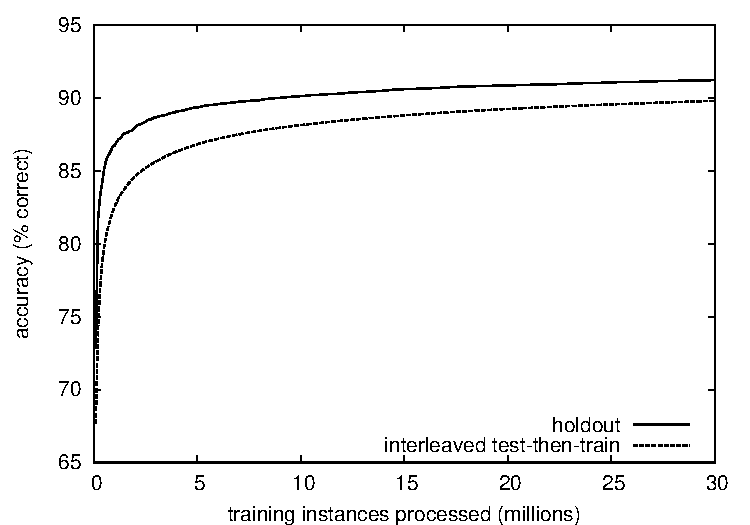
\includegraphics{figures/holdout_vs_interleaved}
\caption{Learning curves produced for the same learning situation by two different evaluation methods, recorded every 100,000 examples.}
\label{fig:holdout_vs_interleaved}
\end{figure}

Figure~\ref{fig:holdout_vs_interleaved} is an example of how learning curves can differ between the two approaches given an identical learning algorithm and data source. The holdout method measures immediate accuracy at a particular point, without memory of previous performance. During the first few million training examples the graph is not smooth. If the test set were small thus unreliable or the algorithm more unstable then fluctuations in accuracy could be much more noticeable. The interleaved method by contrast measures the average accuracy achieved to a given point, thus after 30 million training examples, the generalization accuracy has been measured on every one of the 30 million examples, rather than the independent one million examples used by the holdout. This explains why the interleaved curve is smooth. It also explains why the estimate of accuracy is more pessimistic, because during early stages of learning the model was less accurate, pulling the average accuracy down.

The interleaved method makes measuring estimates of both time and accuracy more difficult. It could be improved perhaps using a modification that introduces exponential decay, but this possibility is reserved for future work. The holdout evaluation method offers the best of both schemes, as the averaged accuracy that would be obtained via interleaved test-then-train can be estimated by averaging consecutive ranges of samples together. Having considered the relative merits of the approaches, the holdout method constitutes the foundation of the experimental framework described next.

\section{Testing Framework}
\label{sec:framework}

\begin{algorithm}
\caption{Evaluation procedure.}
\begin{algorithmic}
\STATE Fix $m_{bound}$, the maximum amount of memory allowed for the model
\STATE Hold out $n_{test}$ examples for testing
\WHILE{further evaluation is desired}
\STATE start training timer
\FOR{$i=1$ to $n_{train}$}
\STATE get next example $e_{train}$ from training stream
\STATE train and update model with $e_{train}$, ensuring that $m_{bound}$ is obeyed
\ENDFOR
\STATE stop training timer and record training time
\STATE start test timer
\FOR{$i=1$ to $n_{test}$}
\STATE get next example $e_{test}$ from test stream
\STATE test model on $e_{test}$ and update accuracy
\ENDFOR
\STATE stop test timer and record test time
\STATE record model statistics (accuracy, size etc.)
\ENDWHILE
\end{algorithmic}
\label{alg:eval}
\end{algorithm}

Algorithm~\ref{alg:eval} lists pseudo-code of the evaluation procedure used for experimental work in this \thesisc. The process is similar to that used by Domingos and Hulten~\cite{vfdt}, the study that was found to have the most thorough evaluation practices of those surveyed in Section~\ref{sec:dsevalsurvey}. It offers flexibility regarding which statistics are captured, with the potential to track many behaviours of interest.

The $n_{train}$ parameter determines how many examples will be used for training before an evaluation is performed on the test set. A set of $n_{test}$ examples is held aside for testing. In the data stream case without concept drift this set can be easily populated by collecting the first $n_{test}$ examples from the stream.

To get reliable timing estimates, $n_{train}$ and $n_{test}$ need to be sufficiently large. In the actual implementation, the timer measured the CPU runtime of the relevant thread, in an effort to reduce problems caused by the multithreaded operating system sharing other tasks. In all experiments, $n_{test}$ was set to one million examples, which helps to measure timing but also ensures reliability of the accuracy estimates, where according to Table~\ref{tab:evalsurvey1} previous studies in the field have typically used a tenth of this amount or even less.

The framework is designed to test an algorithm that tends to accumulate information over time, so the algorithm will desire more memory as it trains on more examples. The algorithm needs to be able to limit the total amount of memory used, thus obey $m_{bound}$, no matter how much training takes place.

\begin{figure}
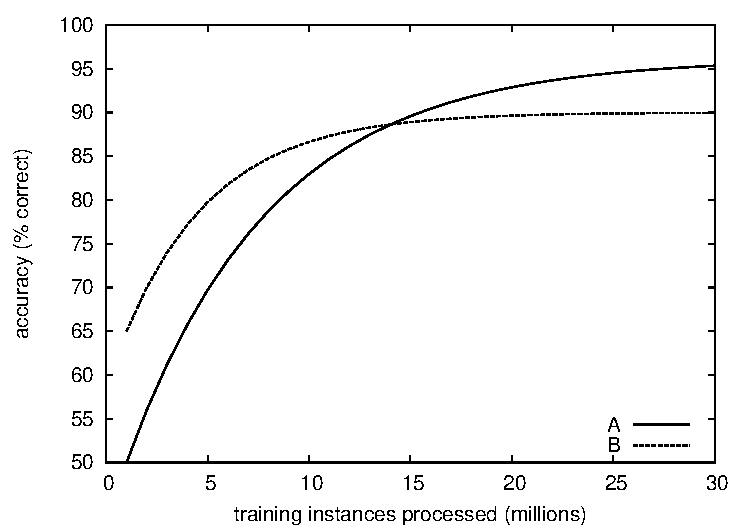
\includegraphics{figures/AvsB}
\caption{Learning curves demonstrating the problem of stopping early.}
\label{fig:learningcurves}
\end{figure}

One of the biggest issues with the evaluation is deciding when to stop training and start testing. In small memory situations, some algorithms will reach a point where they have exhausted all memory and can no longer learn new information. At this point the experiment can be terminated, as the results will not change from that point.

More problematic is the situation where time or training examples are exhausted before the final level of performance can be observed.
Consider Figure~\ref{fig:learningcurves}. Prior to 14 million examples, algorithm B is the clear choice in terms of accuracy, however in the long run it does not reach the same level of accuracy as algorithm A. Which algorithm is actually better depends on the application. If there is a shortage of time or data, algorithm B may be the better choice. Not only this, but if the models are employed for prediction during early stages of learning, then algorithm B will be more useful at the beginning.

To rule out any effect that data order may have on the learning process, the evaluation procedure may be run multiple times, each time with a different set of training data from the same problem. The observations gathered from each run can then be averaged into a single result. An advantage of this approach is that the variance of behaviour can also be observed. Ideally the data between runs will be unique, as is possible with synthetically generated or other abundant data sources. If data is lacking at least the training examples can be reordered.

An ideal method of evaluation would wait until an accuracy plateau is observable for every candidate before termination. It would also run multiple times with different data orders to establish confidence in the results. Unfortunately neither of these scenarios are feasible considering the large amount of experimental work needed. % for this \thesisc.

\BEGINOMIT
To see why this is so, consider the time required to run all of the experiments in this \thesisc. There are 19 different data sources. There are three memory limits, but only two are counted here because experiments terminate early in the smallest environment. There are at least 20 different variants of algorithm being tested, which underestimates the full amount of work by ignoring background experimentation such as performing bias/variance decomposition in Chapter~\ref{chap:improvecompare}.
If ten hours are required per run, the total time required is:
\begin{center}
19 data sets $\times$ 2 environments $\times$ 20 algorithms $\times$ 10 hours = 7600 hours
\end{center}
So a conservative estimate is that 317 days or more than 45 weeks of linear computing time is required to generate the results. Running the evaluation process in parallel is straightforward, so with several machines the practical runtime can be reduced, but not without access to substantial computing resources. Requiring multiple runs or more than ten hours per run will readily inflate the computing time needed.

For this practical reason, all experiments allowed a maximum of ten hours training time. The time required for the entire evaluation process is slightly longer than ten hours due to time required for testing, which is not included in the limit. Aside from algorithms being tested in the smallest memory environment, nearly every algorithm trained for the full ten hour period and could have continued for longer if permitted. The only exceptions were a small number of cases where the most memory-hungry ensemble methods described in Chapter~\ref{chap:improvecompare} became incapable of doing any more work in the memory allowed.

Regarding the problem that terminating evaluation too early can bias results, there are two causes of early termination, shortage of data or shortage of time. Data shortage is avoided by using synthetic data generators thereby having unlimited data. Time shortage is more problematic but as explained it is unreasonable to expect more than ten hours of training per evaluation run, which is considered to be a reasonable amount of time.
\ENDOMIT

The question of when an algorithm is superior to another is decided by looking at the final result recorded after the ten hour evaluation completed. The accuracy results are reported as percentages to two decimal places, and if a method's final accuracy reading in this context is greater than another then it is claimed to be superior. As with other similar studies there is no attempt to strictly analyze the confidence of results, although differences of several percentages are more convincing than fractional differences.

Measuring the standard error of results via multiple runs would enable the confidence of results to be more formally analyzed, but every additional run would multiply time requirements. A less expensive but useful alternative might be to examine differences between algorithms in another way, using McNemar's test~\cite{mcnemar} for example, which can be computed by tracking the agreement between competing methods on each test example. Extra analysis such as this was not considered necessary for this \thesisc, but the idea presents opportunity for future research into evaluation of data stream classification.

\BEGINOMIT
Two factors add informal confidence in the results obtained. Firstly, the class of base algorithm being studied (fully described in Chapter~\ref{chap:hoeffdingtrees}) has low sensitivity to data order, as reported previously~\cite{stresstest,ufft} and confirmed in smaller scale initial experiments. This suggests that even if multiple runs were performed and averaged, the final results would not change very much. Secondly, this study uses test set sizes that are several times larger than the largest used in previous studies, further decreasing the likelihood that methods can achieve high accuracy via chance alone.

The methodology employed is largely consistent with other studies, only on a greater scale. Where previous studies rarely trained on more than several million examples, the ten hour evaluation runs commonly involve several {\em hundreds} of millions of examples. There are two main ways that results are presented, as graphical plots and in tables. Graphical plots are interspersed with the text where they seem appropriate for demonstrating relevant behaviour. Unfortunately, because the graphs need to be of sufficient size to reasonably compare multiple methods, only selected graphs are shown. The space required to print readable graphs of every method on every data source in every environment and every interesting dimension is simply too high to justify.

\begin{figure}
\centering
\begin{tabular}{c@{}c}
\includegraphics[width=0.5\textwidth]{figures/rtcn-r1-400MB_leafacc_vs_examples} &
\includegraphics[width=0.5\textwidth]{figures/rtcn-r1-400MB_leafacc} \\
\end{tabular}
\caption{Example difference between learning curves based on training examples (left) versus training time (right).}
\label{fig:examples_vs_time}
\end{figure}

The information collected during a run of the evaluation procedure can be plotted in several ways to give a visual analysis of an algorithm's behaviour. Of critical interest is the learning curve, as discussed previously, where the accuracy of the algorithm's predictions is plotted against either time or number of training examples.
Previous studies have always plotted learning curves on a per-example basis, rather than a per-time basis that is dependent on the speed of computing hardware. This \thesis uses both styles interchangeably, which can slightly alter the appearance of relationships between methods, see Figure~\ref{fig:examples_vs_time}. The main difference between these styles is that time-based plots have every line spanning almost the full width of the graph rather than having slower methods terminating earlier. Plotted this way, per-example performance is still observable because each sample point represents a fixed number of training examples, such that more frequent points in a line represent more training examples being processed. Often with these graphs the sampling period is purposely adjusted to ensure a reasonable separation between sample points, enhancing readability. Where appropriate the sampling period is noted in the title of the graph. The difference between per-example and per-time plots can be dramatic when the speeds of algorithms differ greatly, such as the example in Figure~\ref{fig:rrbfc_gp} on page~\pageref{fig:rrbfc_gp}.

The graphs are supplemented by tables in Appendix~\ref{chap:detailedResultTables}. The tables cannot convey subtle changes over time like graphs can, but they can report the complete set of end results, allowing comparison of the key results for every method/data source/environment combination. The tables record the final readings at the end of evaluation, which is sufficient information for determining the best methods. Presented in this form the final results are meaningfully summarized in a reasonable amount of space.

The other important property of a learning algorithm besides accuracy is speed. It is important to differentiate learning speed from processing speed. Learning speed refers to the number of examples required to reach a given accuracy level. Processing speed is the rate at which examples are processed, consisting of both training and testing speeds, and can be measured in terms of examples processed per second.
When comparing algorithms, it is the relative time taken on identical hardware that is important, as the absolute times will vary depending on the power of the computing hardware.

The hardware/software environment has a large influence on the results obtained, because a ten hour time limit is completely arbitrary when computing resources are unspecified. The experimental environment was purposely kept consistent for all time-dependent experiments, as follows:
\begin{description}
\item[Hardware:] Intel Core2 6300 CPU running at 1.86Ghz with a 2048KB cache and 1GB of RAM
\item[Software:] Sun Java HotSpot Server VM (build 1.6.0\_01-b06), running under GNU/Linux Fedora core 6
\end{description}
\ENDOMIT

\section{Environments}
\label{sec:environments}

This section defines three environments that may be simulated using memory limits, since memory limits cannot be ignored and can significantly limit capacity to learn from data streams.
Potential practical deployment of data stream classification has been divided into scenarios of increasing memory utilization, from the restrictive {\em sensor} environment, to a typical consumer grade {\em handheld} PDA environment, to the least restrictive environment of a dedicated {\em server}.

Although technology advancements will mean that these environments are something of a moving target, the insights gained about the scalability of algorithms will still be valid. The environments chosen range from restrictive to generous, with an order of magnitude difference between them.

Note that when referring to memory sizes, the traditional meaning of the terms {\em kilobyte} and {\em megabyte} is adopted, such that 1 kilobyte = 1,024 bytes, and 1 megabyte = $1024^2$ bytes = 1,048,576 bytes.

\subsection{Sensor Network}
\label{sec:sensor}

This environment represents the most restrictive case, learning in 100 kilobytes of memory. Because this limit is so restrictive, it is an interesting test case for algorithm efficiency.

Sensor networks~\cite{sensornetworks, sensornetworksbook} are a hot topic of research, and typically the nodes designed for these networks are low power devices with limited resources. In this setting it is often impractical to dedicate more than hundreds of kilobytes to processes because typically such devices do not support much working memory.

When memory limits are in the order of kilobytes, other applications requiring low memory usage also exist, such as specialized hardware in which memory is expensive. An example of such an application is CPU branch prediction, as explored by Fern and Givan~\cite{branchpred}. Another example is a small `packet sniffer' device designed to do real-time monitoring of network traffic~\cite{packetsniff}.

\subsection{Handheld Computer}
\label{sec:handheld}

In this case the algorithm is allowed 32 megabytes of memory. This simulates the capacity of lightweight consumer devices designed to be carried around by users and fit into a shirt pocket.

The ability to do analysis {\em on site} with a handheld device is desirable for certain applications. The papers~\cite{vehicle} and~\cite{stockmarket} describe systems for analysing vehicle performance and stockmarket activity respectively. In both cases the authors describe the target computing hardware as personal handheld devices with 32 megabytes. Horovitz et al.~\cite{gaberroadsafety} describe a road safety application using a device with 64 megabytes.

The promise of ubiquitous computing is getting closer with the widespread use of mobile phones, which with each generation are evolving into increasingly more powerful and multifunctional devices. These too fall into this category, representing large potential for portable machine learning given suitable algorithms. Imielinski and Nath~\cite{wirelessgraffiti} present a vision of this future `dataspace'.

\subsection{Server}
\label{sec:server}

This environment simulates either a modern laptop/desktop computer or server dedicated to processing a data stream. The memory limit assigned in this environment is 400 megabytes. Although at the time of writing this \thesis a typical desktop computer may have several gigabytes of RAM, it is still generous to set aside this much memory for a single process. Considering that several algorithms have difficulty in fully utilizing this much working space, it seems sufficiently realistic to impose this limit.

A practical reason for imposing this limit is that the experiments need to terminate in reasonable time. In cases where memory is not filled by an algorithm it is harder to judge what the behaviour will be in the theoretical limit, but the practical ten hour limit is an attempt to run for sufficient time to allow accuracy to plateau.

There are many applications that fit into this higher end of the computing scale. An obvious task is analysing data arising from the Internet, as either web searches~\cite{webmine}, web usage~\cite{webusage}, site logs~\cite{weblogs} or click streams~\cite{clickstreams}. Smaller scale computer networks also produce traffic of interest~\cite{minenetwork}, as do other telecommunication activities~\cite{telecommunications}, phone call logs for example. Banks may be interested in patterns of ATM transactions~\cite{minebank}, and retail chains and online stores will want details about customer purchases~\cite{ecommerceapp}. Further still, there is the field of scientific observation~\cite{minescientific}, which can be astronomical~\cite{astronomical}, geophysical~\cite{geophysical}, or the massive volume of data output by particle accelerator experiments~\cite{particleaccelerator}. All of these activities are sources of data streams that users will conceivably want to analyze in a server environment.

\section{Data Sources}
\label{sec:datasets}

For the purposes of research into data stream classification there is a shortage of suitable and publicly available real-world benchmark data sets. The UCI ML~\cite{uci} and KDD~\cite{ucikdd} archives house the most common benchmarks for machine learning algorithms, but many of those data sets are not suitable for evaluating data stream classification. The KDD archive has several large data sets, but not classification problems with sufficient examples. The {\em Forest Covertype} data set is one of the largest, and that has less than 600,000 examples.

To demonstrate their systems, several researchers have used private real-world data that cannot be reproduced by others. Examples of this include the web trace from the University of Washington used by Domingos and Hulten to evaluate VFDT~\cite{vfdt}, and the credit card fraud data used by Wang et al.~\cite{cdensemble} and Chu and Zaniolo~\cite{fastlightboost}.

More typically, researchers publish results based on synthetically generated data.
In many of these cases, the authors have invented unique data generation schemes for the purpose of evaluating their algorithm.
Examples include the random tree generator also used to evaluate VFDT, and the custom generators described in Oza and Russell~\cite{ozaexp}, Street and Kim~\cite{sea} and Chu and Zaniolo~\cite{fastlightboost}.
Synthetic data has several advantages---it is easier to reproduce and there is little cost in terms of storage and transmission.
Despite these advantages there is a lack of established and widely used synthetic data streams. 

\begin{table}
\caption{Properties of the data sources.}
\centering
\begin{tabular}{|l|c|c|c|}
\hline
name     &    nominal    &    numeric    &    classes    \\
\hline
{\sc rts/rtsn}    &    10    &    10    &    2    \\
{\sc rtc/rtcn}    &    50    &    50    &    2    \\
{\sc rrbfs}    &    0    &    10    &    2    \\
{\sc rrbfc}    &    0    &    50    &    2    \\
{\sc led}    &    24    &    0    &    10    \\
{\sc wave21}    &    0    &    21    &    3    \\
{\sc wave40}    &    0    &    40    &    3    \\
{\sc genF1-F10}    &    6    &    3    &    2    \\
\hline
\end{tabular}
\label{tab:datasets}
\end{table}

For this \thesisc, the data generators most commonly found in the literature have been collected, and and an extra scheme (RBF) has been introduced. For ease of reference, each data set variation is assigned a short name. The basic properties of each are summarized in Table~\ref{tab:datasets}.

\BEGINOMIT
\subsection{Lack of Real-World Data}
\label{sec:reallack}

The first place to find real-world benchmark data for evaluating machine learning algorithms is the UCI machine learning repository~\cite{uci}. Larger real-world data sets can be found in the UCI KDD archive~\cite{ucikdd}, which was established to serve the needs of larger scale benchmarking.

Table~\ref{tab:ucikddsizes} summarizes the sizes of the data sets in the KDD archive that were found to best suit the task of evaluating classification. The archive has other large data sets that are not considered because they are intended for topics with different requirements such as text categorization and time series classification.

The data set with the most examples is {\em KDD Cup 1999} which has nearly five million training examples. The task is to detect network intrusion attempts. After initial experiments with this data it became clear that it is not a very useful benchmark---it is too easy to achieve near-perfect accuracy, there are many classes with a highly imbalanced distribution of examples between classes, making it hard to discern anything from the accuracies measured for competing methods. Further analysis of the data revealed that there is a high number of repeated examples, such that the number of unique training examples is several times less than the total number of examples specified. Brugger~\cite{kdd99flaw} has expressed concerns that this data set is flawed.

\begin{table}
\caption{Sizes of data sets in UCI KDD archive that are suitable for evaluating classification.}
\centering
\begin{tabular}{|l|r|r|}
\hline					
name	&	attributes	&	training/test examples	\\
\hline					
Census-Income	&	40	&	199,523/99,762	\\
COIL	&	17	&	340	\\
Corel Image	&	89	&	68,040	\\
Forest Covertype	&	54	&	581,012	\\
Insurance Company (COIL2000)	&	86	&	5,822/4,000	\\
Internet Usage	&	71	&	10,108	\\
IPUMS	&	60	&	233,584	\\
KDD Cup 1998	&	481	&	95,412	\\
KDD Cup 1999	&	40	&	4,898,430/311,029	\\
MS Anonymous Web	&	294	&	32,711	\\
\hline					
\end{tabular}
\label{tab:ucikddsizes}
\end{table}

The next largest data set available is {\em Forest Covertype}, a more reasonable classification benchmark. It is not surprising that this data set has been used in several papers on data stream classification~\cite{vfdtc,ozaexp}, given the lack of alternatives.

For the style of evaluation required by this \thesisc, where several hundreds of millions of training examples are required to test genuine ability to handle data streams, these data sets are simply not adequate. The need to rely on artificial data is unfortunate but necessary.
\ENDOMIT

\subsection{Random Tree Generator}
\label{sec:randtrees}

This generator is based on that proposed by Domingos and Hulten~\cite{vfdt}, producing concepts that in theory should favour decision tree learners. It constructs a decision tree by choosing attributes at random to split, and assigning a random class label to each leaf. Once the tree is built, new examples are generated by assigning uniformly distributed random values to attributes which then determine the class label via the tree.

The generator has parameters to control the number of classes, attributes, nominal attribute labels, and the depth of the tree. For consistency between experiments, two random trees were generated and fixed as the base concepts for testing---one {\em simple} and the other {\em complex}, where complexity refers to the number of attributes involved and the size of the tree.

The simple random tree ({\sc rts}) has ten nominal attributes with five values each, ten numeric attributes, two classes, a tree depth of five, with leaves starting at level three and a 0.15 chance of leaves thereafter. The final tree has 741 nodes, 509 of which are leaves.

The complex random tree ({\sc rtc}) has 50 nominal attributes with five values each, 50 numeric attributes, two classes, a tree depth of ten, with leaves starting at level five and a 0.15 chance of leaves thereafter. The final tree has 127,837 nodes, 90,259 of which are leaves.

A degree of noise can be introduced to the examples after generation. In the case of discrete attributes and the class label, a probability of noise parameter determines the chance that any particular value is switched to something other than the original value. For numeric attributes, a degree of random noise is added to all values, drawn from a random Gaussian distribution with standard deviation equal to the standard deviation of the original values multiplied by noise probability.
The streams {\sc rtsn} and {\sc rtcn} are introduced by adding 10\% noise to the respective random tree data streams. It is hoped that experimenting with both noiseless and noisy versions of a problem can give insight into how well the algorithms manage noise.

\subsection{Random RBF Generator}
\label{sec:randrbf}

This generator was devised to offer an alternate concept type that is not necessarily as easy to capture with a decision tree model.

The RBF (Radial Basis Function) generator works as follows:
A fixed number of random centroids are generated. Each center has a random position, a single standard deviation, class label and weight. New examples are generated by selecting a center at random, taking weights into consideration so that centers with higher weight are more likely to be chosen. A random direction is chosen to offset the attribute values from the central point. The length of the displacement is randomly drawn from a Gaussian distribution with standard deviation determined by the chosen centroid. The chosen centroid also determines the class label of the example. This effectively creates a normally distributed hypersphere of examples surrounding each central point with varying densities. Only numeric attributes are generated.

{\sc rrbfs} refers to a simple random RBF data set---100 centers and ten attributes. 
{\sc rrbfc} is more complex---1000 centers and 50 attributes. 
Both are two class problems.

\subsection{LED Generator}
\label{sec:led}

This data source originates from the CART book~\cite{cart}. An implementation in C was donated to the UCI~\cite{uci} machine learning repository by David Aha. The goal is to predict the digit displayed on a seven-segment LED display, where each attribute has a 10\% chance of being inverted. It has an optimal Bayes classification rate of 74\%. The particular configuration of the generator used for experiments ({\sc led}) produces 24 binary attributes, 17 of which are irrelevant.

\subsection{Waveform Generator}
\label{sec:waveform}

This generator shares its origins with {\sc led}, and was also donated by David Aha to the UCI repository. The goal of the task is to differentiate between three different classes of waveform, each of which is generated from a combination of two or three {\em base} waves. The optimal Bayes classification rate is known to be 86\%. There are two versions of the problem. {\sc wave21} has 21 numeric attributes, all of which include noise. {\sc wave40} introduces an additional 19 irrelevant attributes.

\subsection{Function Generator}
\label{sec:genFx}

This generator was introduced by Agrawal et al. in~\cite{dbmine}, and was a common source of data for early work on scaling up decision tree learners~\cite{sliq,sprint,rainforest}.

\begin{table}
\caption{Function generator attributes.}
\centering
\begin{tabular}{|l|l|l|}
\hline
name     &    description    &    values    \\
\hline
{\it salary} & salary & uniformly distributed from 20K to 150K \\
{\it commission} & commission & {\bf if} ({\it salary} $<$ 75K) {\bf then} 0 {\bf else} \\
& & uniformly distributed from 10K to 75K \\
{\it age} & age & uniformly distributed from 20 to 80 \\
{\it elevel} & education level & uniformly chosen from 0 to 4 \\
{\it car} & make of car & uniformly chosen from 1 to 20 \\
{\it zipcode} & zip code of town & uniformly chosen from 9 zipcodes \\
{\it hvalue} & value of house & uniformly distributed \\
& & from 0.5$k$100000 to 1.5$k$100000  \\
& & where $k \in \{1...9\}$ depending on {\it zipcode} \\
{\it hyears} & years house owned & uniformly distributed from 1 to 30  \\
{\it loan} & total loan amount & uniformly distributed from 0 to 500K  \\
\hline
\end{tabular}
\label{tab:agrawalAtts}
\end{table}

The generator produces a stream containing nine attributes, six numeric and three categorical, described in Table~\ref{tab:agrawalAtts}. Although not explicitly stated by the authors, a sensible conclusion is that these attributes describe hypothetical loan applications.

There are ten functions defined for generating binary class labels from the attributes. The functions are listed in Figures~\ref{fig:agrawalFuncs1} and~\ref{fig:agrawalFuncs2}. Presumably these determine whether the loan should be approved. For the experiments the ten functions are used as described, with a perturbation factor of 5\% (referred to as {\sc genF1}-{\sc genF10}). 
Perturbation shifts numeric attributes from their true value, adding an offset drawn randomly from a uniform distribution, the range of which is a specified percentage of the total value range.

\begin{figure}
\begin{enumerate}
\item
{\bf if} ({\it age} $< 40$) $\lor$ ({\it age} $\ge 60$) {\bf then}\\
\hspace*{1em} {\it group} = A\\
{\bf else}\\
\hspace*{1em} {\it group} = B\\
\item
{\bf if} (({\it age} $< 40$) $\land$ ($50000 \le$ {\it salary} $\le 100000$)) $\lor$\\
\hspace*{1em} (($40 \le$ {\it age} $< 60$) $\land$ ($75000 \le$ {\it salary} $\le 125000$)) $\lor$\\
\hspace*{1em} (({\it age} $\ge 60$) $\land$ ($25000 \le$ {\it salary} $\le 75000$)) {\bf then}\\
\hspace*{1em} {\it group} = A\\
{\bf else}\\
\hspace*{1em} {\it group} = B\\
\item
{\bf if} (({\it age} $< 40$) $\land$ ({\it elevel} $\in [0..1$])) $\lor$\\
\hspace*{1em} (($40 \le$ {\it age} $< 60$) $\land$ ({\it elevel} $\in [1..3]$)) $\lor$\\
\hspace*{1em} (({\it age} $\ge 60$) $\land$ ({\it elevel} $\in [2..4]$)) {\bf then}\\
\hspace*{1em} {\it group} = A\\
{\bf else}\\
\hspace*{1em} {\it group} = B \\
\item
{\bf if} (({\it age} $< 40$) $\land$ ({\it elevel} $\in [0..1]$ ?\\
\hspace*{2em} ($25000 \le$ {\it salary} $\le 75000$) : ($50000 \le$ {\it salary} $\le 100000$))) $\lor$\\
\hspace*{1em} (($40 \le$ {\it age} $< 60$) $\land$ ({\it elevel} $\in [1..3]$ ?\\
\hspace*{2em} ($50000 \le$ {\it salary} $\le 100000$) : ($75000 \le$ {\it salary} $\le 125000$))) $\lor$\\
\hspace*{1em} (({\it age} $\ge 60$) $\land$ ({\it elevel} $\in [2..4]$ ?\\
\hspace*{2em} ($50000 \le$ {\it salary} $\le 100000$) : ($25000 \le$ {\it salary} $\le 75000$))) {\bf then}\\
\hspace*{1em} {\it group} = A\\
{\bf else}\\
\hspace*{1em} {\it group} = B\\
\item
{\bf if} (({\it age} $< 40$) $\land$ (($50000 \le$ {\it salary} $\le 100000$) ?\\
\hspace*{2em} ($100000 \le$ {\it loan} $\le 300000$) : ($200000 \le$ {\it loan} $\le 400000$))) $\lor$\\
\hspace*{1em} (($40 \le$ {\it age} $< 60$) $\land$ (($75000 \le$ {\it salary} $\le 125000$) ?\\
\hspace*{2em} ($200000 \le$ {\it loan} $\le 400000$) : ($300000 \le$ {\it loan} $\le 500000$))) $\lor$\\
\hspace*{1em} (({\it age} $\ge 60$) $\land$ (($25000 \le$ {\it salary} $\le 75000$) ?\\
\hspace*{2em} ($30000 \le$ {\it loan} $\le 500000$) : ($100000 \le$ {\it loan} $\le 300000$))) {\bf then}\\
\hspace*{1em} group = A\\
{\bf else}\\
\hspace*{1em} group = B\\
\end{enumerate}
\caption{Generator functions 1-5.}
\label{fig:agrawalFuncs1}
\end{figure}

\begin{figure}
\begin{enumerate}
\setcounter{enumi}{5}
\item
{\bf if} (({\it age} $< 40$) $\land$ ($50000 \le$ ({\it salary} + {\it commission}) $\le 100000$)) $\lor$\\
\hspace*{1em} (($40 \le$ {\it age} $< 60$) $\land$ ($75000 \le$ ({\it salary} + {\it commission}) $\le 125000$)) $\lor$\\
\hspace*{1em} (({\it age} $\ge 60$) $\land$ ($25000 \le$ ({\it salary} + {\it commission}) $\le 75000$)) {\bf then}\\
\hspace*{1em} {\it group} = A\\
{\bf else}\\
\hspace*{1em} {\it group} = B\\
\item
{\bf if} (0.67 $\times$ ({\it salary} + {\it commission}) $-$ 0.2 $\times$ {\it loan} $-$ 20000 $> 0$) {\bf then}\\
\hspace*{1em} {\it group} = A\\
{\bf else}\\
\hspace*{1em} {\it group} = B\\
\item
{\bf if} (0.67 $\times$ ({\it salary} + {\it commission}) $-$ 5000 $\times$ {\it elevel} $-$ 20000 $> 0$) {\bf then}\\
\hspace*{1em} {\it group} = A\\
{\bf else}\\
\hspace*{1em} {\it group} = B\\
\item
{\bf if} (0.67 $\times$ ({\it salary} + {\it commission}) $-$ 5000 $\times$ {\it elevel}\\
\hspace*{1em} $-$ 0.2 $\times$ {\it loan} $-$ 10000 $> 0$) {\bf then}\\
\hspace*{1em} {\it group} = A\\
{\bf else}\\
\hspace*{1em} {\it group} = B\\
\item
{\bf if} ({\it hyears} $\ge 20$) {\bf then}\\
\hspace*{1em} {\it equity} = 0.1 $\times$ {\it hvalue} $\times$ ({\it hyears} $-$ 20)\\
{\bf else}\\
\hspace*{1em} {\it equity} = 0\\
\\
{\bf if} (0.67 $\times$ ({\it salary} + {\it commission}) $-$ 5000 $\times$ {\it elevel}\\
\hspace*{1em} $-$ 0.2 $\times$ {\it equity} $-$ 10000 $> 0$) {\bf then}\\
\hspace*{1em} {\it group} = A\\
{\bf else}\\
\hspace*{1em} {\it group} = B\\
\end{enumerate}
\caption{Generator functions 6-10.}
\label{fig:agrawalFuncs2}
\end{figure}

\section{Generation Speed and Data Size}
\label{sec:genspeed}

During evaluation the data is generated on-the-fly. This directly influences the amount of training examples that can be supplied in any given time period.

\begin{table}
\caption{Generation speed and data size of the streams.}
\centering
\begin{tabular}{|r|r|r|r|r|r|}
\hline		
	&	examples	&		&		&	examples in	&		\\
	&	per second	&		&	bytes per	&	10 hours	&	terabytes in	\\
stream	&	(thousands)	&	attributes	&	example	&	(millions)	&	10 hours	\\
\hline											
{\sc rts}	&	274	&	20	&	168	&	9866	&	1.50	\\
{\sc rtsn}	&	97	&	20	&	168	&	3509	&	0.53	\\
{\sc rtc	}&	19	&	100	&	808	&	667	&	0.49	\\
{\sc rtcn}	&	9	&	100	&	808	&	338	&	0.25	\\
{\sc rrbfs}	&	484	&	10	&	88	&	17417	&	1.39	\\
{\sc rrbfc}	&	120	&	50	&	408	&	4309	&	1.60	\\
{\sc led	}&	260	&	24	&	200	&	9377	&	1.71	\\
{\sc wave21}	&	116	&	21	&	176	&	4187	&	0.67	\\
{\sc wave40}	&	56	&	40	&	328	&	2003	&	0.60	\\
{\sc genF1}	&	527	&	9	&	80	&	18957	&	1.38	\\
{\sc genF2}	&	531	&	9	&	80	&	19108	&	1.39	\\
{\sc genF3}	&	525	&	9	&	80	&	18917	&	1.38	\\
{\sc genF4}	&	523	&	9	&	80	&	18838	&	1.37	\\
{\sc genF5}	&	518	&	9	&	80	&	18653	&	1.36	\\
{\sc genF6}	&	524	&	9	&	80	&	18858	&	1.37	\\
{\sc genF7}	&	527	&	9	&	80	&	18977	&	1.38	\\
{\sc genF8}	&	524	&	9	&	80	&	18848	&	1.37	\\
{\sc genF9}	&	519	&	9	&	80	&	18701	&	1.36	\\
{\sc genF10}	&	527	&	9	&	80	&	18957	&	1.47	\\
\hline											
\end{tabular}
\label{tab:dsspeeds}
\end{table}


The speed of the MOA data generators was measured in the experimental hardware/software environment. The results are shown in Table~\ref{tab:dsspeeds}, where the full speed possible for generating each stream was estimated by timing how long it took to generate ten million examples. The possible speed ranges from around nine thousand examples per second on {\sc rtcn} to over 500 thousand examples per second for the function generators {\sc genF$x$}. The biggest factor influencing speed is the number of attributes being generated, hence the fastest streams are those with the least attributes. The addition of noise to the streams also has a major impact on the speeds---going from {\sc rts} to {\sc rtsn} and from {\sc rtc} to {\sc rtcn} causes the speed to roughly halve, where the only difference between these variants is the addition of noise. 
This result is consistent with the notion that a dominant cost of generating the streams is the time needed to generate random numbers, as adding noise involves producing at least one additional random number per attribute.

In terms of the sizes of the examples, the assumption is made that storage of each attribute and class label requires eight bytes of memory, matching the actual Java implementation where all values are stored as double precision floating point numbers (Section~\ref{sec:javaimpl}). Certain attribute types could be stored more efficiently, but this approach offers maximum flexibility, and storing continuous values in less space would reduce precision.

For example, considering an evaluation period of ten hours, the total number of examples that can be produced at full speed range from around 300 to 19,000 million. With the eight-byte-per-attribute assumption, this translates to between approximately 0.25 to 1.7 terabytes of data. With data volumes of this magnitude the choice of generating data on-the-fly is justified, a solution that is cheaper than finding resources to store and retrieve several terabytes of data.

\BEGINOMIT
\section{Summary}

Aiming to best meet user requirements for data stream classification, the necessity for memory-limited algorithms has been argued. Looking first at prior studies, a comprehensive evaluation framework has been described, testing methods on a scale not previously attempted. The framework is complemented with three simulated memory-limited environments, defined to cover the range of potential deployment scenarios.  A suite of synthetic benchmark data streams have been proposed, and their properties studied. The evaluation framework enables experimental work and comparison of algorithms to be performed throughout the thesis.
\ENDOMIT 
%\chapter{Ensemble Methods}
%\label{ch:ensemblemethods}
\section{Evolving Stream Experimental Setting}
\label{sec:expsetting}
%Advanced analysis of data streams is quickly becoming
%a key area of data mining research as the number of applications
%demanding such processing increases.
%Online mining when such data streams evolve over time,
%that is when concepts drift or change completely,
%is becoming one of the core issues.
%When tackling non-stationary concepts, ensembles of classifiers
%have several advantages over single classifier methods:
%they are easy to scale and parallelize, they can adapt to change
%quickly by pruning under-performing parts of the ensemble, and they
%therefore usually also generate more accurate concept descriptions.
This section proposes a new experimental data stream framework for
studying concept drift using MOA. %, and two new  variants of Bagging.
%Using this new experimental framework,
%an evaluation study
%on synthetic and real-world datasets comprising up to ten
%million examples shows that the new
%ensemble methods perform very well compared to several known methods.
%
%\section{Introduction}
\BEGINOMIT
Conventional knowledge discovery tools assume that the volume of data is such 
that we can store all data in memory or local secondary storage, and there is no limitation on processing time. 
In the {\em Data Stream} model, we have space and time restrictions. Examples of data 
streams are sensoring video streams, network event logs, telephone call records,
credit card transactional flows, etc. 
An important fact is that data may be evolving over time, so we need methods
that adapt automatically. 

The following constraints apply in the Data Stream model:
\begin{enumerate}
\item  Data arrives as a potentially infinite sequence. Thus, it is impossible
 to store it all. Only a small summary can be computed and stored. %, and the rest 
%of the information thrown away. %Even if the information could be stored, 
%it would be infeasible to go over it for further processing.
\item The speed of arrival is fast, so that each particular element has to be 
processed essentially in real time, and then discarded.
\item The distribution generating the items may change over time. Thus, data from 
the past may become irrelevant (or even harmful) for the current prediction.
\end{enumerate}
%Under the Data Stream constraints, 
%The following constraints apply 
%In the Data Stream model,
%data arrives as a potentially infinite sequence, speed of arrival is fast, and 
%the distribution generating the items may change over time. 
Under the constraints of the Data Stream model,
the main properties of an ideal classification method %for mining data streams 
are the following:
high accuracy and fast adaption to change,
low computational cost in both space and time,
theoretical performance guarantees, 
and minimal number of parameters.

These properties may be interdependent: adjusting the time and space used 
by an algorithm can influence accuracy. By storing more pre-computed information, 
such as look up tables, an algorithm can run faster at the expense of
space. An algorithm can also run faster by processing less information, either
by stopping early or storing less, thus having less data to process. The more
time an algorithm has, the more likely it is that accuracy can be
increased.
\ENDOMIT
%Ensemble methods are combinations of several models whose individual predictions 
%are combined in some manner (e.g., averaging or voting) to form a final
%prediction.  Ensemble learning classifiers often have better accuracy and they are easier
%to scale and parallelize than single classifier methods.
A majority of concept drift research in data streams mining is done using
traditional data mining frameworks such as WEKA~\cite{weka}. As the data stream 
setting has constraints that a traditional data mining environment does not, 
we believe that MOA will help to improve the empirical
evaluation of these methods. 

%We present in Section~\ref{frame} a novel framework for evaluation 
%of concept drift. Sections~\ref{hast} and \ref{exp} present two novel ensemble methods
% for handling concept drift,  and a  first comprehensive cross-method comparison. 
%We present conclusions in Section~\ref{discussion}.
%
%{\em Repeatability:} %In accordance to the conference's guideline, the
%source code and executable
%versions of the software, as well as all datasets, will be available from
%MOA's homepage.
%Source code and datasets will be made available at 
%{\tt http://sourceforge.net/projects/moa-datastream}.

In data stream mining, we are interested in three main dimensions:
\begin{itemize}
 \item accuracy 
 \item amount of space necessary or computer memory
 \item the time required to learn from training examples and to predict
\end{itemize}

These properties may be interdependent: adjusting the time and space used 
by an algorithm can influence accuracy. By storing more pre-computed information, 
such as look up tables, an algorithm can run faster at the expense of
space. An algorithm can also run faster by processing less information, either
by stopping early or storing less, thus having less data to process. The more
time an algorithm has, the more likely it is that accuracy can be
increased.

In evolving data streams we are concerned about 

\begin{itemize}
 \item evolution of accuracy
 \item probability of false alarms
 \item probability of true detections
 \item average delay time in detection
\end{itemize}

Sometimes, learning methods do not have change detectors implemented inside,
and then it may be hard to define ratios of false positives and negatives, and
average delay time in detection. In these cases, learning curves may be a useful 
alternative for observing the evolution of accuracy in changing environments.
%or errors when change occurs.

%Under the constraints of the Data Stream model,
To summarize, the main properties of an ideal learning method for mining evolving data streams 
are the following:
high accuracy and fast adaption to change,
low computational cost in both space and time,
theoretical performance guarantees, 
and minimal number of parameters. 


\BEGINOMIT
\section{Experimental framework for concept drift}
\label{sec:expframe}

A data stream environment has different requirements from the traditional 
setting~\cite{Kirkby-PhD}. The most significant are the following: 
\begin{description}
\item[Requirement 1] Process an example at a time, and inspect
 it only once (at most)
\item[Requirement 2] Use a limited amount of memory
\item[Requirement 3] Work in a limited amount of time
\item[Requirement 4] Be ready to predict at any time
\end{description}
\begin{figure}[t]
\begin{center} 
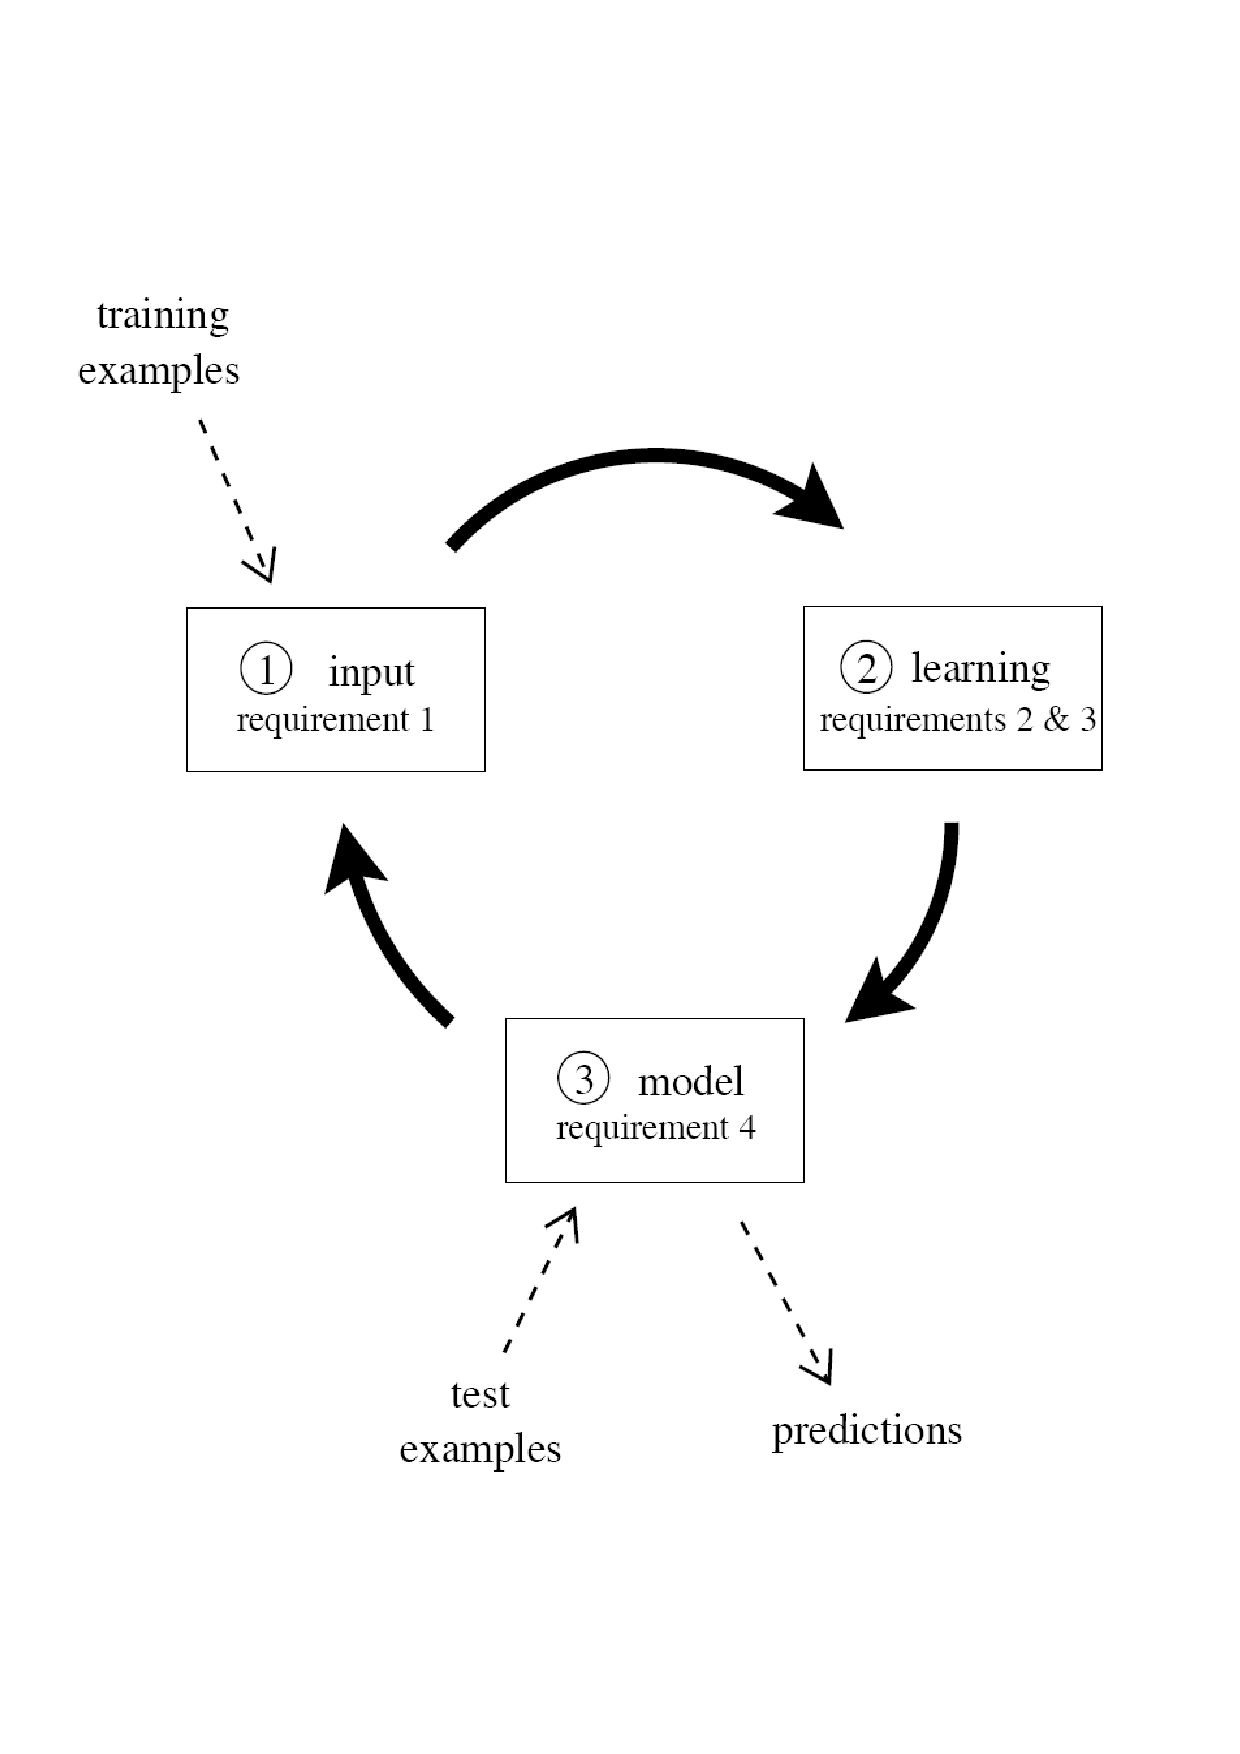
\epsfig{file=Frame, scale=.18}
\end{center} 
\caption{The data stream classification cycle}
\label{fig:cycle}
\end{figure} 
We have to consider these requirements in order to design a new experimental
framework for data streams.
Figure~\ref{fig:cycle} illustrates the typical use of a data stream 
classification algorithm, and how the requirements fit %in. The general model 
%of data stream classification follows these three steps 
in a repeating cycle:
\begin{enumerate}
\item  The algorithm is passed the next available example from the stream
   (requirement 1).
\item  The algorithm processes the example, updating its data structures. It
   does so without exceeding the memory bounds set on it (requirement 2),
   and as quickly as possible (requirement 3).
\item  The algorithm is ready to accept the next example. On request it is
   able to predict the class of unseen examples
   % , and  supply a model that can be used to  
   (requirement 4).
\end{enumerate}


In traditional batch learning the problem of limited data is overcome
by analyzing and averaging multiple models produced with different random
arrangements of training and test data. In the stream setting the problem of
(effectively) unlimited data poses different challenges. One solution involves
taking snapshots at different times during the induction of a model to see how
much the model improves.

The evaluation procedure of a learning algorithm determines which examples
are used for training the algorithm, and which are used to test the model output
by the algorithm. The procedure used historically in batch learning has partly
depended on data size. As data sizes increase, practical
time limitations prevent procedures that repeat training too many times. It is
commonly accepted with considerably larger data sources that it is necessary
to reduce the numbers of repetitions or folds to allow experiments to complete
in reasonable time. 
    When considering what procedure to use in the data stream setting, one of
the unique concerns is how to build a picture of accuracy over time. Two main
approaches arise~\cite{Kirkby-PhD}:
\begin{itemize}
 \item {\bf Holdout}:
When traditional batch learning reaches a scale where cross-validation is too time 
consuming, it is often accepted to instead measure performance on a single holdout
set. This is most useful when the division between train and test sets have
been pre-defined, so that results from different studies can be directly compared. 
%Viewing data stream problems as a large-scale case of batch learning,
%it then follows from batch learning practices that a holdout set is appropriate.
\item {\bf Interleaved Test-Then-Train}:
 Each individual example can be used to test the model
before it is used for training, and from this the accuracy can be incrementally
updated. When intentionally performed in this order, the model is always
being tested on examples it has not seen. This scheme has the advantage that
no holdout set is needed for testing, making maximum use of the available
data. It also ensures a smooth plot of accuracy over time, as each individual
example will become increasingly less significant to the overall average.
%    With this procedure the statistics are updated with every example in the
%stream, and can be recorded at that level of detail if desired. For efficiency
%reasons a sampling parameter can be used to reduce the storage requirements
%of the results, by recording only at periodic intervals like the holdout method.
\end{itemize}
   As data stream classification is a relatively new field, such evaluation 
practices are not nearly as well researched and established as they are
in the traditional batch setting. 
The majority of experimental evaluations use less than one million
training examples. Some papers use more than this, up to ten million examples,
and only very rarely is there any study like Domingos and 
Hulten~\cite{Domingos,hulten-mining}  that is in the order of tens of millions 
of examples. In the context of data streams this is disappointing, because to be
truly useful at data stream classification the algorithms need to be capable of 
handling very large (potentially infinite) streams of examples. Demonstrating 
systems only on small amounts of data does not build a convincing case for capacity
to solve more demanding data stream applications.
%    There are several possible reasons for the general lack of training data for
%evaluation. It could be that researchers come from a traditional machine learning 
%background with entrenched community standards, where results involving
%cross-validation on popular real-world data sets are expected for credibility,
%and alternate practices are less understood. Emphasis on using real-world
%data will restrict the sizes possible, because there is very little data 
%freely available that is suitable for data stream evaluation.
%Another reason could be that the methods are being directly compared with
%batch learning algorithms, as several of the papers do, so the sizes may 
%deliberately be kept small to accommodate batch learning. Hopefully no evaluations
%are intentionally small due to proposed data stream algorithms being too slow
%or memory hungry to cope with larger amounts of data in reasonable time or
%memory, because this would raise serious doubts about the algorithm's
%practical utility.
\ENDOMIT
\BEGINOMIT
    A claim of~\cite{Kirkby-PhD} is that in order to adequately evaluate data stream
classification algorithms they need to be tested on large streams, in the order
of tens of millions of examples where possible, and under explicit memory
limits. Any less than this does not actually test algorithms in a realistically
challenging setting. 
\ENDOMIT

\subsection{Concept Drift Framework}
We present the new experimental framework for concept drift in MOA. Our goal was to introduce
artificial drift to data stream generators in a straightforward way. 
 
The framework approach most similar to the one presented in this Chapter 
 is the one proposed by Narasimhamurthy et al.~\cite{kuncheva07}.
They proposed a general 
framework to generate data simulating
changing environments. Their framework accommodates the %currently favourite 
STAGGER and Moving Hyperplane generation
strategies. % and offers a versatile approach towards
%devising new strategies.
They consider a set of $k$ data sources with known distributions.
As these distributions at the sources are fixed, the data distribution
at time $t$, $D^{(t)}$ is specified through $v_i(t)$, where 
 $v_i(t) \in [0,1]$ specify the extent of the influence of data
source $i$ at time $t$:
$$D^{(t)} = \{v_1(t), v_2(t), \ldots, v_k(t) \}, \sum_{i} v_i(t)= 1$$
Their framework covers gradual and abrupt changes.
Our approach is more concrete, %general,
we begin by dealing 
with a simple scenario: a data stream and two different concepts. Later, we will 
consider the general case with more than one concept drift { events}. 

Considering data streams as data generated from pure distributions, we can model
a concept drift { event} as a weighted combination %a mixture distribution, 
of two pure distributions that characterizes the target concepts before and after
the drift. In our framework, we need to define the probability that every new 
instance of the stream belongs to the new concept after the drift. We will use 
the sigmoid function, as an elegant and practical solution.

\begin{figure}
\begin{tikzpicture}[domain=-2:9]
  \draw[step=2,very thin,color=gray] (-0.1,-0.1) grid (8.2,4.2);
  \draw[->] (-2.2,0) -- (8.2,0) node[right] {$t$};
  \draw[->] (0,-0.2) -- (0,4.2) node[above] {$f(t)$};
  \draw[<->] (2,-0.6) -- (6,-0.6) node[below] {};
  \draw[color=blue!50!black, domain=2:6] plot[id=x]   function{(x-2)}           node[right]{}; %{$f(x) =x$};
  %\draw[color=blue]   plot[id=sin] function{sin(x)}       node[right] {$f(x) = \sin x$};
  \draw[color=red!50!black] plot[id=exp] function{4/(1+exp(4-x))} node[right] {$f(t)$};% = 1/{(1+ \mathrm e^{-s (x-x_0)}})$};
  %\shadedraw[left color=gray,right color=green, draw=green!50!black] (2,0) -- (2.5,0) arc (0:45:.5) -- cycle; 
  \colorlet{anglecolor}{blue!50!black}
  \filldraw[fill=blue!20,draw=anglecolor] (2,0) -- (2.5,0) arc(0:45:.5);
  \draw (2.7,.3) node[anglecolor] {$\alpha$};
  \filldraw[fill=blue!20,draw=anglecolor] (4,2) -- (4.5,2) arc(0:45:.5);
  \draw (4.7,2.3) node[anglecolor] {$\alpha$};

  \draw (4,-0.3) node[] {$t_0$};
  \draw (4,-0.9) node[] {$W$};
  \draw (-0.5,2) node[] {$0.5$};
  \draw (-0.5,4) node[] {$1$};

\end{tikzpicture}
\caption{A sigmoid function $f(t) = 1/{(1+ \mathrm e^{-s (t-t_0)}})$.}
\label{fig:ConceptChange}
\end{figure}
We see from Figure~\ref{fig:ConceptChange} that the sigmoid function 
$$f(t) = 1/{(1+ \mathrm e^{-s (t-t_0)}})$$
has a derivative at the point $t_0$ equal to $f'(t_0) = s/4$. The tangent of angle 
$\alpha$ is equal to this derivative, $\tan \alpha = s/4$. We observe that 
$ \tan \alpha = 1/ W$,
and as $s= 4 \tan \alpha$ then $s=4/W$. So the parameter $s$ in the sigmoid 
gives the length of $W$ and the angle $\alpha$. 
In this sigmoid model we only need to specify two parameters : 
$t_0$ the point of change, and $W$ the length of change.
Note that $$f(t_0+\beta \cdot W)=1 -f(t_0-\beta \cdot W),$$ and  that $f(t_0+\beta \cdot W)$ and $f(t_0-\beta \cdot W)$ 
are constant values that don't depend on $t_0$ and $W$: 
$$f(t_0+W/2) = 1 - f(t_0-W/2) = 1/( 1+ e^{-2}) \approx 88.08 \%$$  
$$f(t_0+W) = 1 - f(t_0-W) = 1/( 1+ e^{-4}) \approx 98.20 \%$$  
$$f(t_0+2W) = 1 - f(t_0-2W) = 1/( 1+ e^{-8}) \approx 99.97 \%$$
\begin{definition} %{\bf ($\oplus$-operation)}\\
Given two data streams $a$, $b$, we define $c = a  \oplus^{W}_{t_0} b$ as the 
data stream built joining the two data streams $a$ and $b$, where
$t_0$ is the point of change, $W$ is the length of change and 
\begin{itemize}
 \item $\Pr[ c(t) = a(t)] = \mathrm e^{-4(t-t_0)/W}/{(1+ \mathrm e^{-4(t-t_0)/W})}$
 \item $\Pr[ c(t) = b(t)] = 1/{(1+ \mathrm e^{-4(t-t_0)/W})}$.
\end{itemize}
\end{definition}
We observe the following properties, if $a \ne b$:
\begin{itemize}
 \item $a \oplus^{W}_{t_0} b \neq b \oplus^{W}_{t_0} a$
 \item $a \oplus^{W}_{t_0} a = a$
 \item $a \oplus^{0}_{0} b = b$
 \item $a \oplus^{W}_{t_0} ( b \oplus^{W}_{t_0} c) \neq (a \oplus^{W}_{t_0}  b)
	 \oplus^{W}_{t_0} c$
 \item $a \oplus^{W}_{t_0} ( b \oplus^{W}_{t_1} c) \approx (a \oplus^{W}_{t_0}  b)
	 \oplus^{W}_{t_1} c$ if $t_0<t_1$ and $W \ll |t_1-t_0|$
\end{itemize}
In order to create a data stream with multiple concept changes, we can build new 
data streams joining different concept drifts:
$$( ( (a \oplus^{W_0}_{t_0}  b) \oplus^{W_1}_{t_1} c) \oplus^{W_2}_{t_2} d ) \ldots $$ 

%and, in the case that all $W$'s are equal

%$$( ( (a \oplus^{W}_{t_0}  b) \oplus^{W}_{t_1} c) \oplus^{W}_{t_2} d ) \ldots $$ 

\subsection{Datasets for concept drift}
\label{datasets}
Synthetic data has several advantages \--- it is easier to reproduce and there is 
little cost in terms of storage and transmission. For this framework, 
the data generators most commonly found in the literature have been collected.

\begin{description} %\subsubsection{SEA Concepts}
 \item[SEA Concepts Generator] This dataset contains abrupt concept drift, 
first introduced  in~\cite{sea}. It is generated using three attributes,
where only the two first attributes are relevant. 
All three attributes have values between 0 and 10.
The points of the dataset are divided into $4$ blocks with different concepts. 
In each block,  the classification is done using $f_1+ f_2 \leq \theta$, 
where $f_1$ and $f_2$ represent the first two attributes 
and $\theta$ is a threshold value. 
The most frequent values are 9, 8, 7 and 9.5 for the data blocks. 
In our framework, SEA concepts are defined as follows:
$$( ( (SEA_9 \oplus^{W}_{t_0}  SEA_8) \oplus^{W}_{2t_0} SEA_7) \oplus^{W}_{3t_0} SEA_{9.5} )  $$ 
 \item[STAGGER Concepts Generator] %\subsubsection{STAGGER Concepts}
%The STAGGER Concepts
They were introduced by Schlimmer and Granger in~\cite{SchlimmerG86}.
The concept description in STAGGER is a collection of elements, where each 
individual element is a Boolean function of attribute-valued pairs that is 
represented by a disjunct of conjuncts. A typical example of a concept description
covering either green rectangles or red triangles can be represented by (shape 
rectangle and colour green) or (shape triangles and colour red).
 \item[Rotating Hyperplane]%\subsubsection{Hyperplane}
%Another frequently used dataset is 
%The rotating hyperplane, 
This dataset was used as testbed for CVFDT 
versus VFDT in~\cite{hulten-mining}. A hyperplane in $d$-dimensional space is the
set of points $x$ that satisfy $$ \sum^{d}_{i=1} w_i x_i = w_0 = \sum^{d}_{i=1} w_i  $$
where $x_i$, is the ith coordinate of $x$. Examples for which $ \sum^{d}_{i=1} w_i x_i \ge w_0 $  
are labeled positive, and examples for which  $ \sum^{d}_{i=1} w_i x_i < w_0 $
are labeled negative. 
Hyperplanes are useful for simulating time-changing concepts, because we can
change the orientation and position of the hyperplane in a
smooth manner by changing the relative size of the weights.
We introduce change to this dataset adding drift to each weight attribute 
 $w_i = w_i + d\sigma$,
where $\sigma$ is the probability that the direction of change is reversed and $d$ is
the change applied to every example.
\item[Random RBF Generator]%\subsubsection{Random RBF Generator}
{ This generator was devised to offer an alternate complex concept type that is not 
straightforward to approximate with a decision tree model.}
%This generator was devised to offer an alternate concept type that is not 
%necessarily as easy to capture with a decision tree model.
The RBF (Radial Basis Function) generator works as follows: A fixed number
of random centroids are generated. Each center has a random position,
a single standard deviation, class label and weight. New examples are 
generated by selecting a center at random, taking weights into consideration so
that centers with higher weight are more likely to be chosen. A random 
direction is chosen to offset the attribute values from the central point. The
length of the displacement is randomly drawn from a Gaussian distribution
with standard deviation determined by the chosen centroid. The chosen 
centroid also determines the class label of the example. This effectively creates a
normally distributed hypersphere of examples surrounding each central point
with varying densities. Only numeric attributes are generated. 
Drift is introduced by moving the centroids with constant speed. This speed is
initialized by a drift parameter.
\BEGINOMIT
 \item[LED Generator]%\subsubsection{LED Generator}
This data source originates from the CART book~\cite{cart93}. An implementation in
C was donated to the UCI~\cite{uci} machine learning repository by David Aha. The
goal is to predict the digit displayed on a seven-segment LED display, where
each attribute has a 10\% chance of being inverted. It has an optimal Bayes
classification rate of 74\%. The particular configuration of the generator used
for experiments (led) produces 24 binary attributes, 17 of which are irrelevant.
 \item[Waveform Generator]%\subsubsection{Waveform Generator}
It shares its origins with { LED}, and was also donated by David Aha
to the UCI repository. The goal of the task is to differentiate between three
different classes of waveform, each of which is generated from a combination
of two or three base waves. The optimal Bayes classification rate is known
to be 86\%. There are two versions of the problem, wave21 which has 21 numeric
attributes, all of which include noise, and wave40 which introduces an additional 19
irrelevant attributes.
 \item[Function Generator] %subsubsection{Function Generator}
It was introduced by Agrawal et al. in~\cite{agrawal}, and was a common
source of data for early work on scaling up decision tree learners~\cite{dbmine,sliq, sprint,rainforest}.
The generator produces a stream containing nine attributes, six numeric and 
three categorical. Although not explicitly stated by the authors, a sensible 
conclusion is that these attributes describe hypothetical loan applications.
There are ten functions defined for generating binary class labels from the
attributes. 
Presumably these determine whether the loan should be approved. 
\ENDOMIT
 \end{description}
Data streams may be considered infinite sequences of $(x,y)$ where $x$ is the feature vector and $y$
the class label. Zhang et al.~\cite{Zhang08} observe that $ p(x,y) = p(x|t) \cdot p(y|x) $ and categorize concept drift in two types:
\begin{itemize}
 %\item 
\item \emph{Loose Concept Drifting (LCD)} when concept drift is caused only by the change of the class prior probability $p(y|x)$, %\item 
\item  \emph{Rigorous Concept Drifting (RCD)} when concept drift is caused by the change of the class prior probability $p(y|x)$ and the conditional probability $p(x|t)$  
\end{itemize}

Note that the Random RBF Generator has RCD drift, and the rest of the dataset generators have LCD drift.

\subsubsection{Real-World Data}


%The first place to find real-world benchmark data for evaluating machine learning 
%algorithms is the UCI machine learning repository~\cite{Adult}. Larger real-world
%data sets can be found in the UCI KDD archive~\cite{UCIKDD}, which was established to
%serve the needs of larger scale benchmarking.

%The data set with the most examples is KDD Cup 1999 which has nearly
%five million training examples. The task is to detect network intrusion attempts. 
%After initial experiments with this data it became clear that it is not
%a very useful benchmark-it is too easy to achieve near-perfect accuracy, there
%are many classes with a highly imbalanced distribution of examples between
%classes, making it hard to discern anything from the accuracies measured for
%competing methods.
It is not easy to find large real-world datasets
for public benchmarking, especially with substantial concept change. %big real-world datasets.
The UCI machine learning repository~\cite{uci} contains some real-world benchmark 
data for evaluating machine learning techniques. 
We will consider three : Forest Covertype, Poker-Hand, and Electricity.
%algorithms is the UCI machine learning repository~\cite{Adult}.
%In the experiments with  real datasets we use two UCI 
%datasets~\cite{Adult} Adult and Poker-Hand from the UCI repository of machine learning databases.
\begin{description}
 \item[Forest Covertype dataset] It contains 
the forest cover type for 30 x 30 meter cells obtained from US Forest Service (USFS) Region 2 Resource Information System (RIS) data. 
It contains $581,012$ instances and $54$ attributes, and
it has been used
in several papers on data stream classification~\cite{vfdtc, ozaexp}.
 \item[Poker-Hand dataset] %The Poker-Hand dataset 
It consists of $1,000,000$ %1,025,010 
instances and $11$ attributes.
Each record of the Poker-Hand dataset is an example of a hand consisting of five playing cards drawn from a standard deck of $52$. Each card is described using two attributes (suit and rank), for a total of $10$ predictive attributes. There is one Class attribute that describes the ``Poker Hand''. The order of cards is important, which is why there are $480$ possible Royal Flush hands instead of $4$.
\item[Electricity dataset] 
Another widely used dataset is the Electricity Market Dataset described by M. Harries \cite{Harries} 
and used by Gama \cite{Gama}. 
This data was collected from the Australian New South Wales Electricity Market. 
In this market, the prices are not fixed and are affected by demand and supply of the market. 
The prices in this market are set every five minutes. 
The ELEC2 dataset contains $45,312$ instances. %dated from $7$ May $1996$ to $5$ December $1998$. 
Each example of the dataset refers to a period of $30$ minutes, i.e. there are $48$ instances
for each time period of one day. %Each example on the dataset has 5 fields, the
%day of week, the time stamp, the NSW electricity demand, the Vic electricity
%demand, the scheduled electricity transfer between states and the class label.
The class label identifies the change of the price related to a moving average of
the last $24$ hours. The class level only reflect deviations of the price on a one
day average and removes the impact of longer term price trends. 
 \end{description}
 
The size of these datasets is small, compared to tens of millions of training examples of synthetic datasets: $45,312$ for ELEC2 dataset, $581,012$ for CoverType, and $1,000,000$ for Poker-Hand.
Another important fact is that we do not know when drift occurs or if there is any drift. We may simulate RCD concept drift, joining the three datasets, merging attributes, and supposing that each dataset corresponds to a different concept.
$$ \textrm{CovPokElec} =  (\textrm{CoverType} \oplus^{5,000}_{581,012} \textrm{Poker}) \oplus^{5,000}_{1,000,000} \textrm{ELEC2} $$ 

%For the style of evaluation required by this paper, where several hundreds
%of millions of training examples are required to test genuine ability to handle
%data streams, these data sets are simply not adequate. The need to rely on
%artificial data is unfortunate but necessary.
\BEGINOMIT
\subsection{MOA Experimental Framework}
\label{ssec:moa}
{\bf M}assive {\bf O}nline {\bf A}nalysis (MOA)~\cite{MOA} is a
framework for online learning from continuous %supplies of examples, such as 
data streams.
The data stream evaluation framework and most of the classification algorithms evaluated in this thesis
were implemented in the Java programming language extending the MOA framework.
MOA includes a collection of offline and online methods as well as tools for evaluation. 
In particular, it implements boosting, bagging, and Hoeffding Trees, all %both 
with and without Na{\"\i}ve Bayes classifiers at the leaves. 
%MOA  graphical user interface is shown in Figure~\ref{fig:moagui}.
%However, a command line interface is also available.

%\begin{figure}[t]
%\begin{center} 
%\epsfig{file=MOATL, scale=0.3}
%\end{center} 
%\caption{MOA Graphical User Interface}
%\label{fig:moagui}
%\end{figure} 

MOA is related to WEKA, the Waikato
Environment for Knowledge Analysis~\cite{weka}, which is an award-winning open-source 
workbench containing implementations of a wide range of batch machine 
learning methods. WEKA is also written in Java. The main benefits
of Java are portability, where applications can be run on any platform with
an appropriate Java virtual machine, and the strong and well-developed support 
libraries. Use of the language is widespread, and features such as the
automatic garbage collection help to reduce programmer burden and error.

    One of the key data structures used in MOA is the description of an example
from a data stream. This structure borrows from WEKA, where an example is
represented by an array of double precision floating point values. This provides
freedom to store all necessary types of value \--- numeric attribute values can be
stored directly, and discrete attribute values and class labels are represented
by integer index values that are stored as floating point values in the array.
Double precision floating point values require storage space of 64 bits, or 8
bytes. This detail can have implications for memory usage. %utilization.
\ENDOMIT%\cleardoublepage{}
\part{Stationary Data Stream Learning} 
\chapter{Hoeffding Trees}
\label{chap:hoeffdingtrees} 

%This chapter describes the Hoeffding tree algorithm, chosen as the base method on which to build the MOA experimental framework of data stream classification. The reasons for choosing this algorithm are elaborated below. Most importantly, the algorithm is an ideal starting point, as it is innovative and effective at high speed data stream classification, yet it also presents opportunities for improvement.

Hoeffding trees were introduced by Domingos and Hulten in the paper ``Mining High-Speed Data Streams''~\cite{vfdt}. They refer to their implementation as {\em VFDT}, an acronym for {\bf V}ery {\bf F}ast {\bf D}ecision {\bf T}ree learner. In that paper the Hoeffding tree algorithm is the basic theoretical algorithm, while VFDT introduces several enhancements for practical implementation. In this \thesis  the term {\it Hoeffding tree} refers to any variation or refinement of the basic principle, VFDT included.

In further work Domingos and Hulten went on to show how their idea can be generalized~\cite{mineabitrarydb}, claiming that any learner based on discrete search can be made capable of processing a data stream. The key idea depends on the use of {\it Hoeffding bounds}, described in Section~\ref{sec:hoeffdingbounds}. While from this point of view VFDT may only be one instance of a more general framework, not only is it the original example and inspiration for the general framework, but because it is based on decision trees it performs very well, for reasons given shortly.

Hoeffding trees are being studied because they represent current state-of-the-art for classifying high speed data streams. The algorithm fulfills the requirements necessary for coping with data streams while remaining efficient, an achievement that was rare prior to its introduction. Previous work on scaling up decision tree learning produced systems such as {\it SLIQ}~\cite{sliq}, {\it SPRINT}~\cite{sprint} and {\it RAINFOREST}~\cite{rainforest}. These systems perform batch learning of decision trees from large data sources in limited memory by performing multiple passes over the data and using external storage. Such operations are not suitable for high speed stream processing.

Other previous systems that are more suited to data streams are those that were designed exclusively to work in a single pass, such as the incremental systems {\it ID5R}~\cite{id5r} and its successor {\it ITI}~\cite{iti}, and other earlier work on incremental learning. Systems like this were considered for data stream suitability by Domingos and Hulten, who found them to be of limited practical use. In some cases these methods require more effort to update the model incrementally than to rebuild the model from scratch. In the case of ITI, all of the previous training data must be retained in order to revisit decisions, prohibiting its use on large data sources. 

The Hoeffding tree induction algorithm induces a decision tree from a data stream incrementally, briefly inspecting each example in the stream only once, without need for storing examples after they have been used to update the tree. The only information needed in memory is the tree itself, which stores sufficient information in its leaves in order to grow, and can be employed to form predictions at any point in time between processing training examples.

Domingos and Hulten present a proof guaranteeing that a Hoeffding tree will be `very close' to a decision tree learned via batch learning. This shows that the algorithm can produce trees of the same quality as batch learned trees, despite being induced in an incremental fashion. This finding is significant because batch learned decision trees are among the best performing machine learning models.
The classic decision tree learning schemes {\em C4.5}~\cite{c4.5} and {\em CART}~\cite{cart}, two similar systems that were independently developed, are widely recognised by the research community and regarded by many as de facto standards for batch learning.

There are several reasons why decision tree learners are highly regarded. They are fairly simple, the decision tree model itself being easy to comprehend. This high level of {\it interpretability} has several advantages. The decision process induced via the learning process is transparent, so it is apparent {\it how} the model works. Questions of {\it why} the model works can lead to greater understanding of a problem, or if the model manages to be successful without truly reflecting the real world, can highlight deficiencies in the data used.

The quest for accuracy means that interpretability alone will not guarantee widespread acceptance of a machine learning model. Perhaps the main reason decision trees are popular is that they are consistently accurate on a wide variety of problems. The classic decision tree systems recursively split the multi-dimensional data into smaller and smaller regions, using greedily chosen axis-orthogonal splits. This divide-and-conquer strategy is simple yet often successful at learning diverse concepts.

Another strong feature of decision trees is their efficiency.
With $n$ examples and $m$ attributes, page 197 of~\cite{weka} shows that the average cost of basic decision tree induction is $O(mn \log n)$, ignoring complexities such as numeric attributes and subtree raising. A more detailed study of tree induction complexity can be found in~\cite{dtcomplexity}.
The cost of making a decision is $O($tree depth$)$ in the worst case, where typically the depth of a tree grows logarithmically with its size.

For the batch setting, recent studies~\cite{mlcomparison} have shown that single decision trees are no longer the best off-the-shelf method. However, they are competitive when used as base models in ensemble methods. 
For this reason, ensemble methods employing Hoeffding trees are explored later in chapters~\ref{chap:improvebackground}. %and~\ref{chap:improvecompare}. 

\section{The Hoeffding Bound for Tree Induction}
\label{sec:hoeffdingbounds}

Each internal node of a standard decision tree contains a test to divide the examples, sending examples down different paths depending on the values of particular attributes. 
The crucial decision needed to construct a decision tree is when to split a node, and with which example-discriminating test.        
If the tests used to divide examples are based on a single attribute value, as is typical in classic decision tree systems, then the set of possible tests is reduced to the number of attributes.
So the problem is refined to one of deciding which attribute, if any, is the best to split on.

There exist popular and well established criteria for selecting decision tree split tests. 
Perhaps the most common is {\it information gain}, used by C4.5.
Information gain measures the average amount of `purity' that is gained in each subset of a split. The purity of the subsets is measured using {\em entropy}, which for a distribution of class labels consisting of fractions ${p}_{1},{p}_{2},...,{p}_{n}$ summing to 1, is calculated thus:

\begin{equation} \label{eq:entropy}
\mathrm{entropy}({p}_{1},{p}_{2},...,{p}_{n}) = \sum_{i=1}^{n} -{p}_{i} \log_{2} {p}_{i}
\end{equation}

Gain in information is measured by subtracting the weighted average entropy of the subsets of a split from the entropy of the class distribution before splitting. Entropy is a concept from information theory that measures the amount of information conveyed by a message in {\em bits}. Throughout this \thesis  the splitting criterion is assumed to be information gain, but this does not rule out other methods. As pointed out by Domingos and Hulten, other similar methods such as the Gini index used by CART can be just as equally applied.

The estimated information gain resulting from a split on each attribute is the heuristic used to guide split decisions. In the batch learning setting this decision is straightforward, as the attribute with the highest information gain over all of the available and applicable training data is the one used. How to make the same (or very similar) decision in the data stream setting is the innovation contributed by Domingos and Hulten. They employ the Hoeffding bound~\cite{hoeffding}, otherwise known as an additive Chernoff bound.

The Hoeffding bound states that with probability $1 - \delta$, the true mean of a random variable of range $R$ will not differ from the estimated mean after $n$ independent observations by more than:

\begin{equation} \label{eq:hbound}
\epsilon = \sqrt{\frac{R^{2}\ln(1/\delta)}{2n}}
\end{equation}

This bound is useful because it holds true regardless of the distribution generating the values, and depends only on the range of values, number of observations and desired confidence. A disadvantage of being so general is that it is more conservative than a distribution-dependent bound.
An alternative bound has been suggested by Jin and Agrawal~\cite{nip}.
The Hoeffding bound formulation is well founded and works well empirically, so tighter bounds are not explored in this \thesisc. 

For the purposes of deciding which attribute to split on, the random variable being estimated is the difference in information gain between splitting on the best and second best attributes. For example, if the difference in gain between the best two attributes is estimated to be 0.3, and $\epsilon$ is computed to be 0.1, then the bound guarantees that the maximum possible change in difference will be 0.1. From this the smallest possible difference between them in the future must be at least 0.2, which will always represent positive separation for the best attribute.

For information gain the range of values ($R$) is the base 2 logarithm of the number of possible class labels. With $R$ and $\delta$ fixed, the only variable left to change the Hoeffding bound ($\epsilon$) is the number of observations ($n$). As $n$ increases, $\epsilon$ will decrease, in accordance with the estimated information gain getting ever closer to its true value.

A simple test allows the decision, with confidence $1 - \delta$, that an attribute has superior information gain compared to others---when the difference in observed information gain is more than $\epsilon$. This is the core principle for Hoeffding tree induction, leading to the following algorithm.

\section{The Basic Algorithm}
\label{sec:basicalgorithm}

\begin{algorithm}
\caption{Hoeffding tree induction algorithm.}
\begin{algorithmic}[1]
\STATE Let $HT$ be a tree with a single leaf (the root)
\FORALL{training examples}
\STATE Sort example into leaf $l$ using $HT$
\STATE Update sufficient statistics in $l$
\STATE Increment $n_l$, the number of examples seen at $l$
\IF{$n_l$ $mod$ $n_{min}$ $= 0$ {\bf and} examples seen at $l$ not all of same class}
\STATE Compute $\overline{G}_{l}(X_{i})$ for each attribute
\STATE Let $X_{a}$ be attribute with highest $\overline{G}_{l}$
\STATE Let $X_{b}$ be attribute with second-highest $\overline{G}_{l}$
\STATE Compute Hoeffding bound $\epsilon = \sqrt{\frac{R^{2}\ln(1/\delta)}{2n_{l}}}$
\IF{$X_{a} \ne X_{\emptyset}$ {\bf and} ($\overline{G}_{l}(X_{a}) - \overline{G}_{l}(X_{b}) > \epsilon$ {\bf or} $\epsilon < \tau$)}
\STATE Replace $l$ with an internal node that splits on $X_{a}$
\FORALL{branches of the split}
\STATE Add a new leaf with initialized sufficient statistics
\ENDFOR
\ENDIF
\ENDIF
\ENDFOR
\end{algorithmic}
\label{alg:ht}
\end{algorithm}

Algorithm~\ref{alg:ht} lists pseudo-code for inducing a Hoeffding tree from a data stream.
Line 1 initializes the tree data structure, which starts out as a single root node. Lines 2-18 form a loop that is performed for every training example.

Every example is filtered down the tree to an appropriate leaf, depending on the tests present in the decision tree built to that point (line 3). This leaf is then updated (line 4)---each leaf in the tree holds the sufficient statistics needed to make decisions about further growth. The sufficient statistics that are updated are those that make it possible to estimate the information gain of splitting on each attribute. Exactly what makes up those statistics is discussed in Section~\ref{sec:suffstats}.
Line 5 simply points out that $n_l$ is the example count at the leaf, and it too is updated. Technically $n_l$ can be computed from the sufficient statistics.

For efficiency reasons the code block from lines 6-17 is only performed periodically, every $n_{min}$ examples for a particular leaf, and only when necessary, when a mix of observed classes permits further splitting. The delayed evaluation controlled by $n_{min}$ is discussed in Section~\ref{sec:graceperiod}.

Lines 7-11 perform the test described in the previous section, using the Hoeffding bound to decide when a particular attribute has won against all of the others. $G$ is the splitting criterion function (information gain) and $\overline{G}$ is its estimated value. In line 11 the test for $X_{\emptyset}$, the null attribute, is used for pre-pruning (Section~\ref{sec:preprune}). The test involving $\tau$ is used for tie-breaking (Section~\ref{sec:tiebreak}).

If an attribute has been selected as the best choice, lines 12-15 split the node, causing the tree to grow. Preventing the tree from using too much memory is the topic of Section~\ref{sec:memmanage}.

\subsection{Split Confidence}
\label{sec:splitconf}

The $\delta$ parameter used in the Hoeffding bound is one minus the desired probability that the correct attribute is chosen at every point in the tree. Because a high likelihood of correctness is desired, with probability close to one, this parameter is generally set to a small value. For the experiments described throughout the \thesisc,  $\delta$ is set to the VFDT default of $10^{-7}$.

\begin{figure}
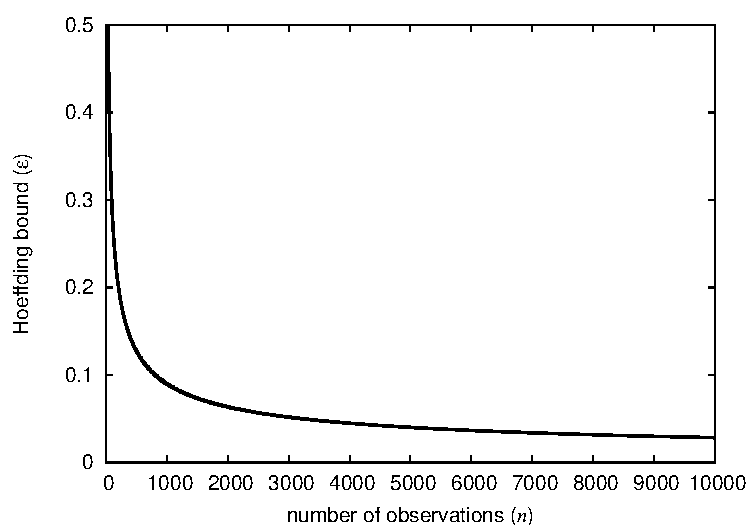
\includegraphics{figures/hoeffdingbound2class}
\caption{Hoeffding bound on a two-class problem with default parameters.}
\label{fig:hbound}
\end{figure}

Figure~\ref{fig:hbound} shows a plot of the Hoeffding bound using the default parameters for a two-class problem ($R = \mathrm{log}_{2}(2) = 1$, $\delta = 10^{-7}$). The bound rapidly drops to below 0.1 within the first one thousand examples, and after ten thousand examples is less than 0.03. This means that after ten thousand examples the calculated information gain of an attribute needs to be 0.03 greater than the second best attribute for it to be declared the winner.

\subsection{Sufficient Statistics}
\label{sec:suffstats}

The statistics in a leaf need to be sufficient to enable calculation of the information gain afforded by each possible split. Efficient storage is important---it is costly to store information in the leaves, so storing unnecessary information would result in an increase in the total memory requirements of the tree.

For attributes with discrete values, the statistics required are simply counts of the class labels that apply for each attribute value. If an attribute has $v$ unique attribute values and there are $c$ possible classes, then this information can be stored in a table with $vc$ entries. The node maintains a separate table per discrete attribute. Updating the tables simply involves incrementing the appropriate entries according to the attribute values and class of the training example.
Table~\ref{tab:leafsuffstats} on page~\pageref{tab:leafsuffstats}, used as an example when looking at prediction methods, shows what such tables can look like.

Continuous numeric attributes are more difficult to summarize. Chapter~\ref{chap:numericatts} is dedicated to this topic.

\subsection{Grace Period}
\label{sec:graceperiod}

It is computationally costly to evaluate the information gain of attributes after each and every training example. Given that a single example will have little influence on the results of the calculation, it is sensible to wait for more examples before re-evaluating. The $n_{min}$ parameter, or grace period, dictates how many examples since the last evaluation should be seen in a leaf before revisiting the decision.

This has the attractive effect of speeding up computation while not greatly harming accuracy. The majority of training time will be spent updating the sufficient statistics, a lightweight operation. Only a fraction of the time will splits be considered, a more costly procedure. The worst impact that this delay will have is a slow down of tree growth, as instead of splitting as soon as possible, a split will delayed by as much as $n_{min}-1$ examples.

For experimentation $n_{min}$ is fixed at 200, the default setting found in the original paper~\cite{vfdt}. Figure~\ref{fig:rrbfc_gp} shows the impact this setting has on the accuracy of trees induced from the {\sc rrbfc} data. From the plot in the top-left it would appear that considering split decisions after every training example does improve the accuracy of the tree, at least within the first 30 million training examples shown on this data. From an accuracy per example perspective, the non grace period tree is superior. The plot to the top-right shows more of the picture, where each tree was allowed ten hours to grow, the tree that had $n_{min}$ set to 200 was able to process almost 800 million examples and achieve significantly better accuracy within that time than the tree lacking a grace period. The plot to the bottom-left shows the total number of examples that were processed over that time---without a grace period 30 million examples in ten hours were possible, with a grace period approximately 25 times more examples were processed in the same time period. Viewing accuracy per time spent in the bottom-right plot makes the advantage of using a grace period clear.

\begin{figure}
\centering
\begin{tabular}{c@{}c}
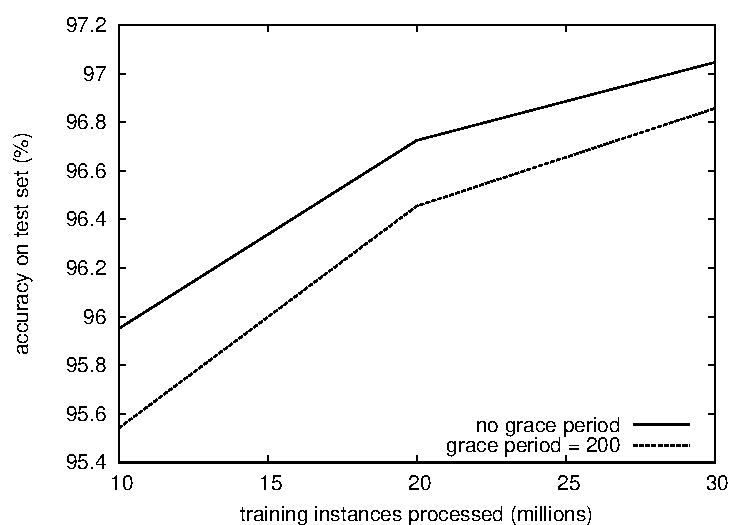
\includegraphics[width=0.5\textwidth]{figures/gp_rrbfc_acc_examples} &
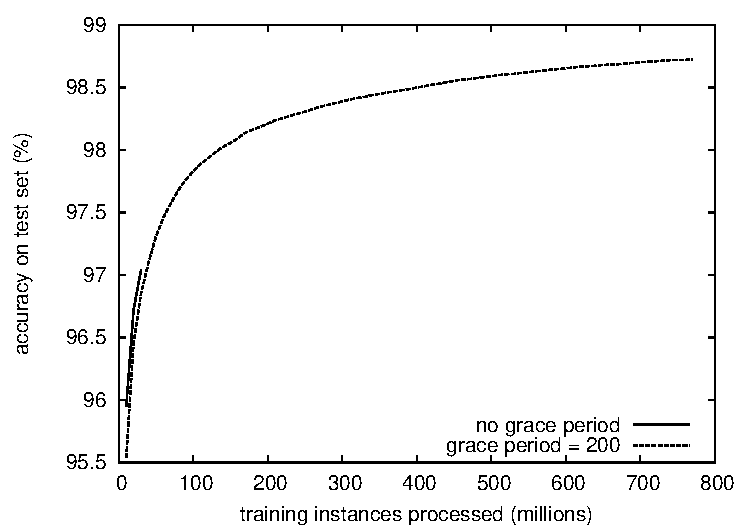
\includegraphics[width=0.5\textwidth]{figures/gp_rrbfc_acc_examples_fullrange} \\
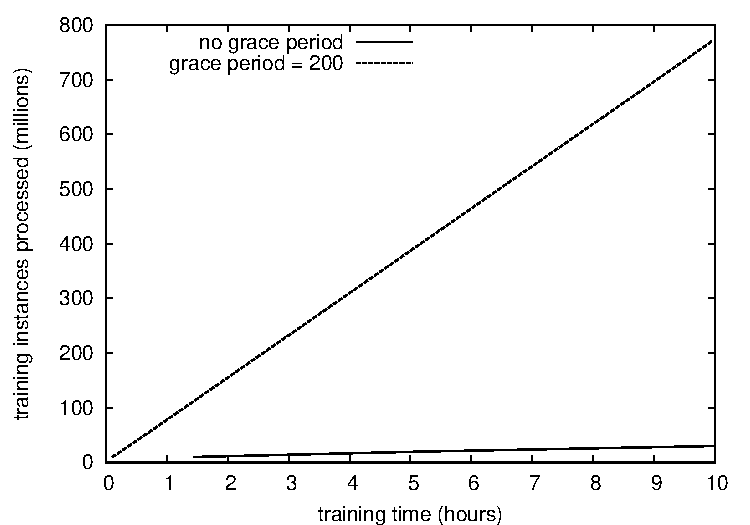
\includegraphics[width=0.5\textwidth]{figures/gp_rrbfc_time} &
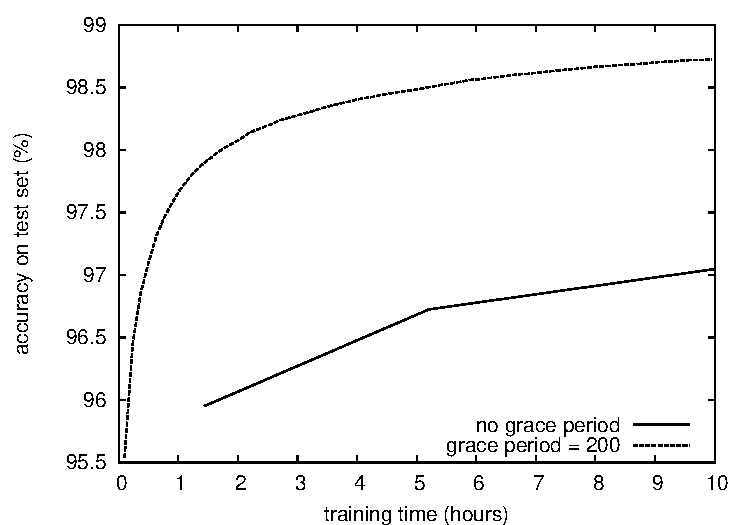
\includegraphics[width=0.5\textwidth]{figures/gp_rrbfc_acc_time} \\
\end{tabular}
\caption{Effect of grace period on the {\sc rrbfc} data with a 32MB memory limit.}
\label{fig:rrbfc_gp}
\end{figure}


\subsection{Pre-pruning}
\label{sec:preprune}

It may turn out more beneficial to not split a node at all. The Hoeffding tree algorithm detects this case by also considering the merit of no split, represented by the null attribute $X_{\emptyset}$. A node is only allowed to split when an attribute looks sufficiently better than $X_{\emptyset}$, by the same Hoeffding bound test that determines differences between other attributes.

All of the Hoeffding tree implementations used in experiments for this \thesis  had pre-pruning enabled, but revisiting some of the results without pre-pruning yielded %no noticeable differences.
no noticeable difference in size, speed or accuracy of trees.
This raises questions about the value of pre-pruning---it does not appear to be harmful and has theoretical merit, but in practice may not have an effect. This question remains open and is not further explored by this \thesisc. 

Pre-pruning in the stream setting is not a permanent decision as it is
in batch learning. Nodes are prevented from splitting until it appears
that a split will be useful, so in this sense, the memory management
strategy of disabling nodes (Section~\ref{sec:memmanage}) can also be viewed as a form of pre-pruning. Conventional knowledge about decision tree pruning is that pre-pruning can often be premature and is not as commonly used as post-pruning approaches. One reason for premature pre-pruning could be lack of sufficient data, which is not a problem in abundant data streams.

In the batch learning setting it is very easy to induce a tree that perfectly fits the training data but does not generalize to new data. This problem is typically overcome by post-pruning the tree. On non-concept drifting data streams such as those described here, it is not as critical to prevent overfitting via post-pruning as it is in the batch setting. If concept drift were present, active and adaptive post-pruning could be used to adjust for changes in concept, a topic outside the scope of this \thesisc. 

\subsection{Tie-breaking}
\label{sec:tiebreak}

A situation can arise where two or more competing attributes cannot be separated. A pathological case of this would be if there were two attributes with identical values. No matter how small the Hoeffding bound it would not be able to separate them, and tree growth would stall.

If competing attributes are equally good, and are superior to some of the other split options, then waiting too long to decide between them can do more harm than good to the accuracy of the tree. It should not make a difference which of the equal competitors is chosen. To alleviate this situation, Domingos and Hulten introduce a tie breaking parameter, $\tau$. If the Hoeffding bound is sufficiently small, that is, less than $\tau$, then the node is split on the current best attribute regardless of how close the next best option is.

The effect of this parameter can be viewed in a different way. Knowing the other variables used in the calculation of the Hoeffding bound, it is possible to compute an upper limit on the number of examples seen by a leaf before tie-breaking intervenes, forcing a split on the best observed attribute at that point. The only thing that can prevent tie-breaking is if the best option turns out to be not splitting at all, hence pre-pruning comes into effect.

$\tau$ is set to the literature default of 0.05 for the experiments. With this setting on a two-class problem, ties will be broken after 3,224 examples are observed. With $n_{min}$ being set to 200, this will actually be delayed until 3,400 examples.

Tie-breaking can have a very significant effect on the accuracy of trees produced. An example is given in Figure~\ref{fig:tiebreak_rrbfc}, where without tie-breaking the tree grows much slower, ending up around five times smaller after 700 million training examples and taking much longer to come close to the same level of accuracy as the tie-breaking variant.

\begin{figure}
\centering
\begin{tabular}{c@{}c}
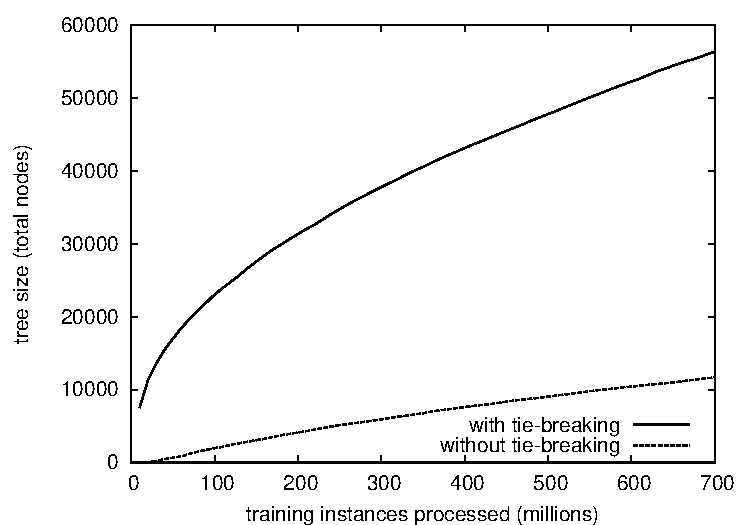
\includegraphics[width=0.5\textwidth]{figures/tiebreak_rrbfc_size} &
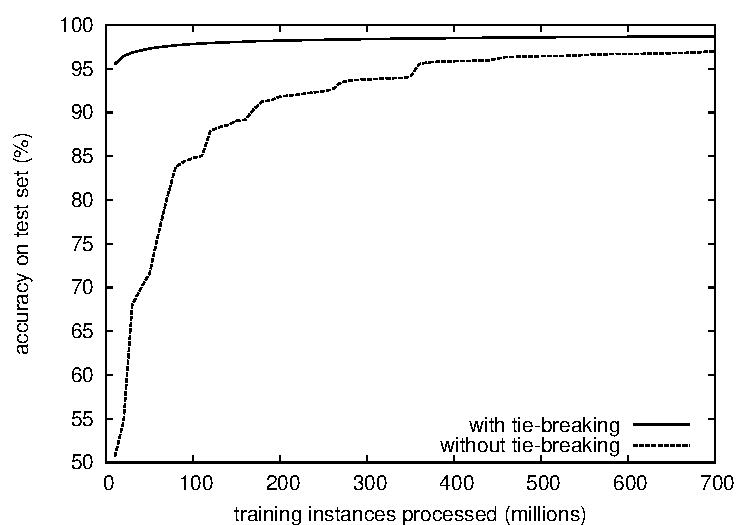
\includegraphics[width=0.5\textwidth]{figures/tiebreak_rrbfc_acc} \\
\end{tabular}
\caption{Effect of tie-breaking on the {\sc rrbfc} data with a 32MB memory limit.}
\label{fig:tiebreak_rrbfc}
\end{figure}


\subsection{Skewed Split Prevention}
\label{sec:skewedsplits}

There is another element present in the Hoeffding tree experimental implementation that is not mentioned in the pseudo-code. It is a small enhancement to split decisions that was first introduced by Gama et al.~\cite{vfdtc} and originally formulated for two-way numeric splits. In this \thesis  the concept has been generalized to apply to any split including splits with multiple branches.

The rule is that a split is only allowed if there are at least two branches where more than $p_{min}$ of the total proportion of examples are estimated to follow the branch. The $p_{min}$ threshold is an arbitrary parameter that can be adjusted, where a default value of 1\% seems to work well enough. This prevents a highly skewed split from being chosen, where less than 1\% of examples go down one path and over 99\% of examples go down another. Such a split can potentially look attractive from an information gain perspective if it increases the purity of the subsets, but from a tree growth perspective is rather spurious.

In many cases this rule has no effect on tree classification accuracy, but Figure~\ref{fig:skewedsplits_rrbfc} shows it can have a positive effect in some cases.

\begin{figure}
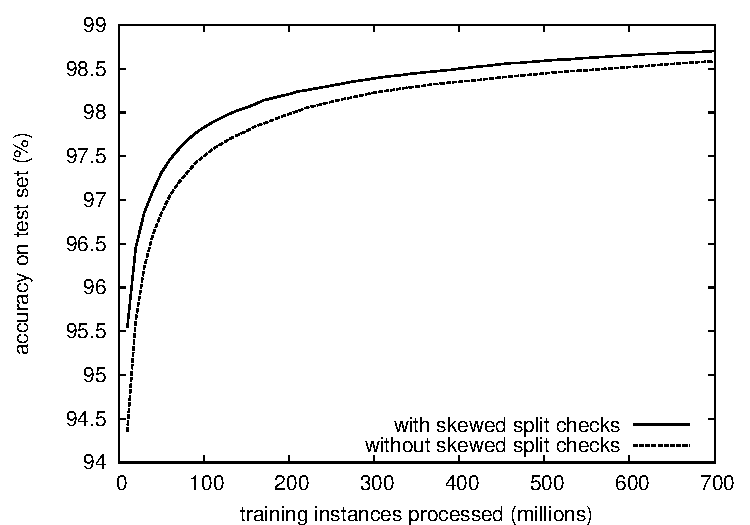
\includegraphics{figures/skewedsplits_rrbfc_acc}
\caption{Effect of preventing skewed splits on the {\sc rrbfc} data with a 32MB memory limit.}
\label{fig:skewedsplits_rrbfc}
\end{figure}

\section{Memory Management}
\label{sec:memmanage}

The basic algorithm as described will continue to split the tree as needed, without regard for the ever-increasing memory requirements. This \thesis  argues that a core requirement of data stream algorithms is the ability to limit memory usage. To limit Hoeffding tree memory size, there must be a strategy that limits the total number of nodes in the tree.
The node-limiting strategy used follows the same principles that Domingos and Hulten introduced for the VFDT system.

When looking at the memory requirements of a Hoeffding tree, the dominant cost is the storage of sufficient statistics in the leaves. Figure~\ref{fig:leaves_bytes} is an example of how closely, in unbounded memory, the number of leaves in a tree can reflect its actual memory requirements. Section~\ref{sec:fastsizeest} describes in more detail how this relationship is exploited to efficiently estimate the actual memory size of the tree based on node counts.

\begin{figure}
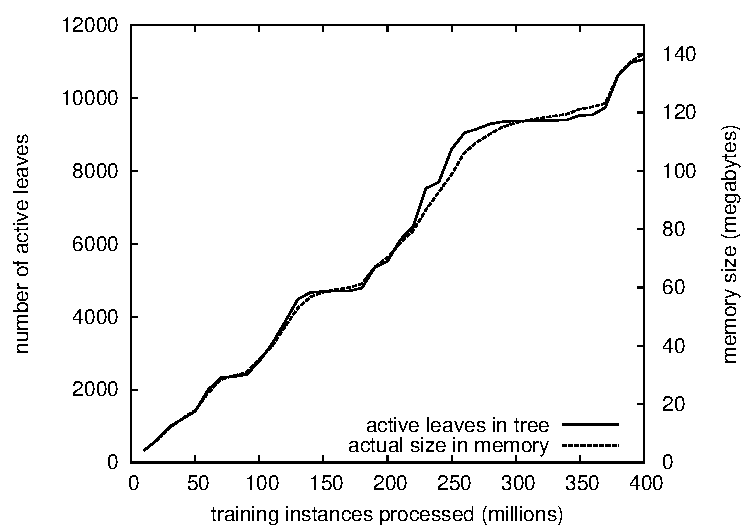
\includegraphics{figures/leaves_bytes}
\caption{The size of an unbounded tree in memory is closely related to how many active leaves it has. This growth pattern occurs when learning a Hoeffding tree on the {\sc led} data.}
\label{fig:leaves_bytes}
\end{figure}

The main idea behind the memory management strategy is that when faced with limited memory, some of the leaves can be {\em deactivated}, such that their sufficient statistics are discarded. Deciding which leaves to deactivate is based on a notion of how promising they look in terms of yielding accuracy gains for the tree.

In VFDT, the least promising nodes are defined to be the ones with the lowest values of $p_{l}e_{l}$, where $p_{l}$ is the probability that examples will reach a particular leaf $l$, and $e_{l}$ is the observed rate of error at $l$. Intuitively this makes sense, the leaves considered most promising for further splitting are those that see a high number of examples and also make a high number of mistakes. Such leaves will be the largest contributors to error in classification, so concentrating effort on splitting these nodes should see the largest reduction in error.

The implementation created for this \thesis  measures the `promise' of leaves in an equivalent and straightforward way. Every leaf in the tree is capable of returning the full count of examples it has observed for each class since creation. The promise of a node is defined as the total remaining number of examples that have been seen to fall outside the currently observed majority class. Like VFDT's $p_{l}e_{l}$ measure, this estimates the potential that a node has for misclassifying examples. If $n$ is the number of examples seen in a leaf, and $E$ is the number of mistakes made by the leaf, and $N$ is the total number of examples seen by the tree, then $p_{l}e_{l} = n/N \times E/n = E/N$. Promise is measured using $E$, which is equivalent to using $E/N$, as $N$ is constant for all leaves.

To make memory management operate without introducing excessive runtime overhead, the size is estimated approximately whenever new nodes are introduced to the tree using the method described in Section~\ref{sec:fastsizeest}. Periodically, a full and precise memory check is performed. This is done after every {\em mem-period} training examples are processed, where {\em mem-period} is a user defined constant. The periodic memory check calculates the actual memory consumption of the tree, a potentially costly process.

After checking memory usage, if there happen to be inactive nodes or if the maximum memory limit has been exceeded then a scan of the leaves is performed. The leaves are ordered from least promising to most promising, and a calculation is made based on the current sizes of the nodes to determine the maximum number of active nodes that can be supported. Once this threshold has been established, any active leaves found below the threshold are deactivated, and any inactive leaves above the threshold are reactivated. This process ensures that the tree actively and dynamically adjusts its focus on growing the most promising leaves first, while also keeping within specified memory bounds.

\begin{figure}
\centering
\framebox{
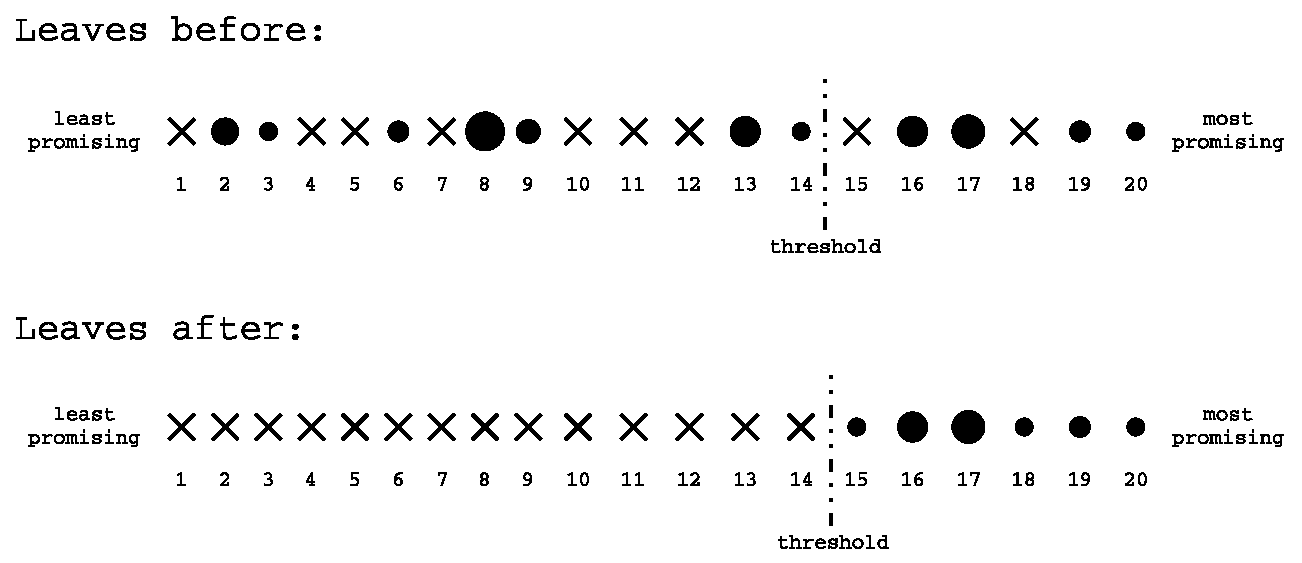
\includegraphics[width=0.95\linewidth]{figures/memmanage}
}
\caption{The memory management strategy employed after leaves of a tree have been sorted in order of {\em promise}. Dots represent {\em active} leaves which store sufficient statistics of various size, crosses represent {\em inactive} leaves which do not store sufficient statistics.}
\label{fig:memmanage}
\end{figure}

Figure~\ref{fig:memmanage} illustrates the process. The top part of the illustration shows twenty leaf nodes from a hypothetical Hoeffding tree ordered from least to most promising. The size of active nodes in memory can differ due to the method used to track numeric attributes (Chapter~\ref{chap:numericatts}) and when the sufficient statistics of poor attributes have been removed (Section~\ref{sec:pooratts}). The sizes of the dots indicate the sizes of the active nodes, and inactive nodes are represented by crosses. Based on the average size of the active nodes and the total memory allowed, the threshold is determined in this case to allow a maximum of six active nodes. The bottom row shows the outcome after memory management is complete---below the threshold, the least promising nodes have all been deactivated, and above the threshold nodes 15 and 18 have been activated to make all of the most promising ones active.

\begin{figure}
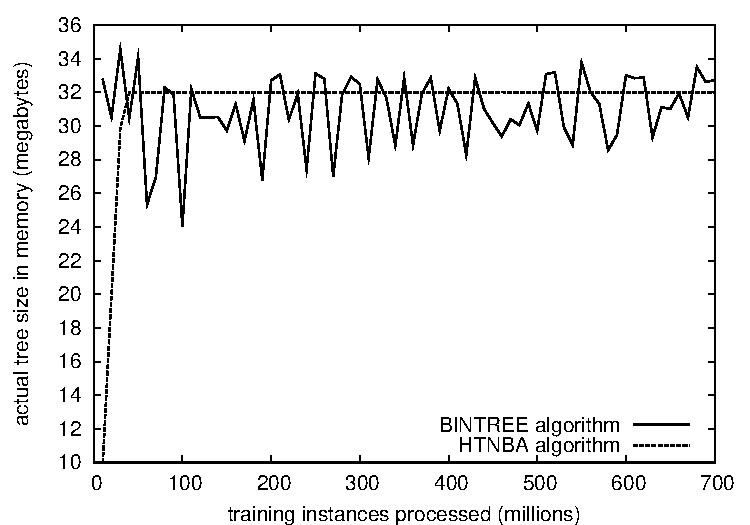
\includegraphics{figures/memslip}
\caption{How closely two algorithms manage to obey a memory limit of 32 megabytes on the {\sc led} data.}
\label{fig:memslip}
\end{figure}

For methods where the relative size between internal nodes, active leaves and inactive leaves is relatively constant this method is very effective at keeping the tree within a memory bound. For some methods where summary statistics in leaves can grow rapidly and vary substantially in size, such as the exhaustive binary tree numeric handling method ({\sc bintree}) described in Chapter~\ref{chap:numericatts}, it is less successful in maintaining a strict memory bound. In these cases, the tree's memory usage has a chance to creep beyond the limit in the period between memory checks, but will be brought back to the memory limit as soon as the next check is performed. Figure~\ref{fig:memslip} demonstrates a case of memory `creep' that occurred in the experiments---the target memory limit is 32 megabytes, and for efficiency the memory usage is only precisely measured every one hundred thousand examples, that is, {\em mem-period} = 100,000. In this case, the memory used by {\sc bintree} temporarily exceeds the memory bounds by as much as three megabytes or roughly 9\%, but all the while fluctuating close to and more often further below the desired bound. The figure compares this with the memory requirements of the {\sc htnba} variant on the same data, a much more stable method described in Chapter~\ref{chap:predstrat}. The majority of the Hoeffding tree variants tested in the experiments exhibit stable memory behaviour, so most cases look like this, where the memory plot over time hits the target precisely before completely flattening out.

While the dominant storage cost is incurred for active nodes, limiting their number will eventually cause the size of internal nodes and inactive leaves to become significant. A point will be reached where no further growth of the tree can occur without the memory limit being exceeded. Once this stage is reached, all leaves of the tree will be made inactive, and the tree will no longer be able to grow.

One element of memory usage that has not yet been accounted for is the temporary working space needed to perform operations on the tree. Implemented in a modern computer language, update and prediction operations will make several function calls, and will store values and pointers in local memory, typically using some space on a working stack. This cost, which will partly depend on implementation details, is assumed to be small and bounded such that it is insignificant compared to storage of the tree itself.

\subsection{Poor Attribute Removal}
\label{sec:pooratts}

An additional strategy for saving space was also suggested by Domingos and Hulten~\cite{vfdt}. This strategy aims to reduce the size of the sufficient statistics in each leaf. 
The idea is to discard sufficient statistics for individual attributes when it looks very unlikely that they will be selected.
When new leaves are formed, all attributes are considered as candidates for splitting. During every evaluation round that does not result in a decision to split, attributes are determined to be poor if their information gain is less than the gain of the current best attribute by more than the Hoeffding bound. According to the bound, such attributes are unlikely to be selected in that particular node of the tree, so the information tracking them in the leaf is discarded and they are ignored in split decisions from that point onward.

This strategy is not as powerful as full node deactivation, the best it can do is help to reduce the average size of leaf nodes. Theoretically this should benefit the accuracy of trees, because it will allow more leaves to remain active in limited memory. In practice the gains appear to be slight, as demonstrated in Figure~\ref{fig:pooratts}, where on {\sc rrbfc} the plot to the left shows a significant increase in the number of leaves allowed to remain active in a 32MB limit, while the plot to the right shows that this only translates to a small gain in accuracy. In this case the accuracy is measured when the tree makes predictions using standard majority class prediction. Removing poor attributes will affect the enhanced prediction methods described in Chapter~\ref{chap:predstrat}, where this is discussed further.

\begin{figure}
\centering
\begin{tabular}{c@{}c}
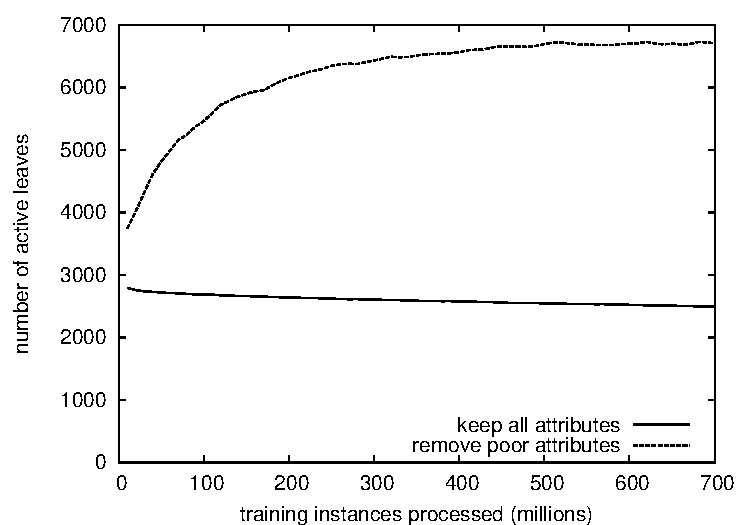
\includegraphics[width=0.5\textwidth]{figures/pooratt_active} &
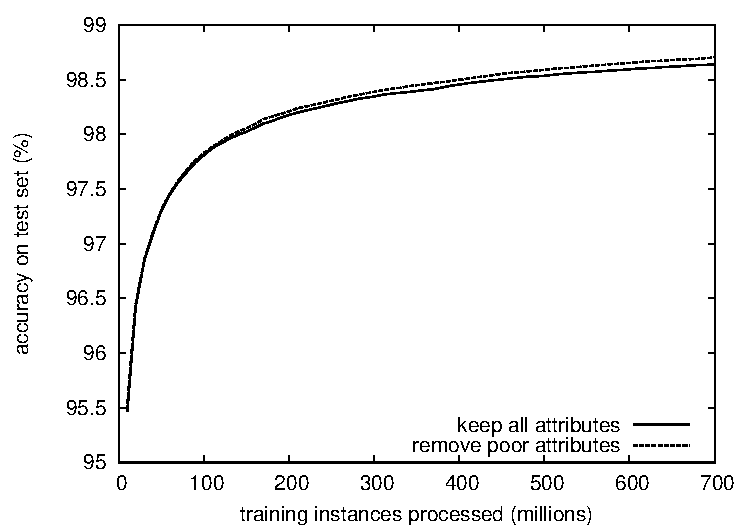
\includegraphics[width=0.5\textwidth]{figures/pooratt_acc} \\
\end{tabular}
\caption{Effect of poor attribute removal on {\sc rrbfc} data with a 32MB limit.}
\label{fig:pooratts}
\end{figure}


\section{MOA Java Implementation Details}
\label{sec:javaimpl}

%The data stream evaluation framework and all algorithms evaluated in this \thesis  were implemented in the Java programming language. The framework is named {\em MOA}, an acronym for {\bf M}assive {\bf O}nline {\bf A}nalysis, and has evolved during the course of developing this \thesisc. 

% MOA is related to {\em WEKA}\footnote{The moa and the weka are both birds native to New Zealand. The weka is a cheeky bird of similar size to a chicken. The moa was a large ostrich-like bird, an order of magnitude larger than a weka, that was hunted to extinction for its meat.}, the {\bf W}aikato {\bf E}nvironment for {\bf K}nowledge {\bf A}nalysis~\cite{weka}, which is an award-winning\footnote{Recipient of the 2005 SIGKDD Data Mining and Knowledge Discovery Service Award.} open-source workbench containing implementations of a wide range of batch machine learning methods. WEKA is also written in Java. The main benefits of Java are portability, where applications can be run on any platform with an appropriate Java virtual machine, and the strong and well-developed support libraries. Use of the language is widespread, and features such as the automatic garbage collection help to reduce programmer burden and error.

One of the key data structures used in MOA is the description of an example from a data stream. This structure borrows from WEKA, where an example is represented by an array of double precision floating point values. This provides freedom to store all necessary type of values---numeric attribute values can be stored directly, and discrete attribute values and class labels are represented by integer index values that are stored as floating point values in the array. Double precision floating point values require storage space of 64 bits, or 8 bytes. This detail can have implications for memory utilization.

A challenge in developing the system has been measuring the total sizes of objects in memory. Java deliberately hides details about how memory is allocated. This frees programmers from the burden of maintaining direct memory pointers that is otherwise typical in C programming, reducing dependence on a particular platform and eliminating a common source of error. The downside is that it makes the task of precisely measuring and limiting the memory usage of algorithms more difficult. 

Early attempts at memory measurement revolved around exploiting Java's automatic {\em serialization} mechanism. It is easy to make all objects capable of being serialized, which means that they can be written out as a flat stream of bytes to be reconstructed later. The idea was to measure the size of the serialized stream of an object, which must be related to its true size in memory. The measuring process can be performed with minimum overhead by writing the object to a dummy stream that allocates no memory but instead simply counts the total number of bytes requested during write operations. It turns out that this method, while suitable for approximate relative measurement of object size, was not precise enough to achieve the level of control needed to confidently evaluate the algorithms. Often the true size of objects would be underestimated, so that
even if the Java virtual machine was allocated a generous amount of memory it could still run into problems, strongly indicating that the serialized size estimates were inadequate.

Fortunately the release of Java 5 introduced a new mechanism allowing access to more accurate memory allocation measurements that are implementation specific. The {\em instrumentation} interface is harder to access as it requires extra work to be done by invoking the virtual machine with an {\em agent}, but once correctly set up can be queried for the size of a single object in memory. The size returned does not account for other sub-objects that are referenced, so it will not immediately return the total size of a complex data structure in memory, but this can be achieved by implementing additional code that uses {\em reflection} to traverse an entire data structure and compute the total size.

\begin{figure}
\begin{verbatim}
...
public static class ClassA implements Serializable {
   public int fieldA;
}
public static class ClassB implements Serializable {
   public int fieldA, fieldB;
}
public static class ClassC implements Serializable {
   public int fieldA, fieldB, fieldC;
}
public static class ClassD implements Serializable {
   public int fieldA, fieldB, fieldC, fieldD;
}
public static class ClassE implements Serializable {
   public int fieldA, fieldB, fieldC, fieldD, fieldE;
}
public static void main(String[] args) throws Exception {
   ClassA classAobject = new ClassA();
   ClassB classBobject = new ClassB();
   ClassC classCobject = new ClassC();
   ClassD classDobject = new ClassD();
   ClassE classEobject = new ClassE();
   ClassA[] classAarray = new ClassA[100];
   ClassB[] classBarray = new ClassB[100];
   ClassC[] classCarray = new ClassC[100];
   ClassD[] classDarray = new ClassD[100];
   ClassE[] classEarray = new ClassE[100];
   for (int i = 0; i < 100; i++) {
      classAarray[i] = new ClassA();
      classBarray[i] = new ClassB();
      classCarray[i] = new ClassC();
      classDarray[i] = new ClassD();
      classEarray[i] = new ClassE();
   }
   System.out.println("classAobject serialized size = "
                      + serializedByteSize(classAobject)
                      + " instrument size = "
                      + instrumentByteSize(classAobject));
   ...
\end{verbatim}
\caption{Java code testing two methods for measuring object sizes in memory.}
\label{fig:javacode}
\end{figure}

\begin{figure}
\begin{verbatim}
classAobject serialized size = 72 instrument size = 16
classBobject serialized size = 85 instrument size = 16
classCobject serialized size = 98 instrument size = 24
classDobject serialized size = 111 instrument size = 24
classEobject serialized size = 124 instrument size = 32
classAarray serialized size = 1124 instrument size = 2016
classBarray serialized size = 1533 instrument size = 2016
classCarray serialized size = 1942 instrument size = 2816
classDarray serialized size = 2351 instrument size = 2816
classEarray serialized size = 2760 instrument size = 3616
\end{verbatim}
\caption{Output from running the code in Figure~\ref{fig:javacode}.}
\label{fig:javaoutput}
\end{figure}

The Java code listing in Figure~\ref{fig:javacode} tests the two size measuring methods. Five simple Java classes possessing an increasing number of fields are measured, along with the size of those objects when replicated 100 times in an array. Figure~\ref{fig:javaoutput} displays the result of running the test in the same software environment as all of the experimental results reported in this \thesisc.  The results show that the serialization method has a tendency to over-estimate the size of single small objects in memory, which would be expected due to the overhead that must be required to completely describe a serialized stream. Interestingly though, serialization also has a tendency to underestimate the size of a collection of objects, where for example the size of the \verb|classA| array is estimated to be almost half of the instrumentation size. This behaviour explains the problems encountered when trying to rely on serialization measurements for experiments. The problem lies in hidden implementation details that make the serialization mechanism store information more efficiently than the virtual machine. The instrumentation measurements expose other effects that could not otherwise be predicted. There appears to be some form of {\em byte padding} effect present, where an object with a single integer field (4 bytes worth) requires the same space as one with two fields (16 bytes in both cases). The reason for this will be a technical decision on behalf of the virtual machine implementation, perhaps a byte alignment issue for the sake of efficiency. Whatever the reason, this discovery serves to highlight the value of an accurate measurement mechanism, enabling the ability to account for such nuances that could not be anticipated otherwise. 

\subsection{Fast Size Estimates}
\label{sec:fastsizeest}

For the Java implementation, the number of active and inactive nodes in a Hoeffding tree are used to estimate the total true size of the tree in memory. The node counts of a growing tree are easily maintained---whenever a new node is added an appropriate counter can be incremented, and when activating or deactivating leaves the counters are appropriately adjusted.

The size estimation procedure requires that actual measurements be performed every so often to establish and refine the parameters used for future estimation. The actual byte size in memory is measured ({\em trueSize}), along with the average byte size of individual active nodes ({\em activeSize}) and inactive nodes  ({\em inactiveSize}). From this an extra parameter is calculated:

\begin{equation} \label{eq:fastmemoverhead}
overhead = \frac{trueSize}{active \times activeSize + inactive \times inactiveSize}
\end{equation}

To increase the precision of the estimate the number of internal nodes in the tree, of similar size to inactive nodes, could also be included in the calculation. The implementation did not do this however, as the procedure described worked sufficiently well.

The estimated overhead is designed to account for the internal nodes of the tree, small inaccuracies in the node estimation procedure and any other structure associated with the tree that has otherwise not been accounted for, bringing the final estimate closer to the true value. Once these values are established, the actual byte size of the tree can be quickly estimated based solely on the number of active and inactive nodes in the tree:

\begin{equation} \label{eq:fastmemcalc}
size = (active \times activeSize + inactive \times inactiveSize) \times overhead
\end{equation}

This calculation can be quickly performed whenever the number of inactive or active leaves changes, sparing the need to do a complete rescan and measurement of the tree after every change.

\BEGINOMIT
\section{Summary}

Representing one of the current best techniques for learning to classify examples in data streams, the basic algorithm for inducing decision trees from data streams via Hoeffding bounds has been described, and various parameter settings discussed. The challenge of memory management has been described, and some issues with the actual implementation in Java examined. 
Two important aspects of Hoeffding trees have not been covered, as they are studied in the following chapters.
Creating decisions based on continuous numeric attributes is studied in Chapter~\ref{chap:numericatts}. How the tree forms predictions is studied in Chapter~\ref{chap:predstrat}. 

\ENDOMIT



 %\cleardoublepage{}
\chapter{Numeric Attributes}
\label{chap:numericatts} 

The ability to learn from numeric attributes is very useful because many attributes needed to describe real-world problems are most naturally expressed by continuous numeric values. The decision tree learners C4.5 and CART successfully handle numeric attributes. Doing so is straightforward, because in the batch setting every numeric value is present in memory and available for inspection. A learner that is unable to deal with numeric attributes creates more burden for users. The data must first be pre-processed so that all numeric attributes are transformed into discrete attributes, a process referred to as {\it discretization}. Traditionally discretization requires an initial pass of the data prior to learning, which is undesirable for data streams.

The original Hoeffding tree algorithm demonstrated only how discrete attribute values could be handled. Domingos and Hulten~\cite{vfdt} claim that the extension to numeric attributes:

\begin{quote}
...is immediate, following the usual method of allowing tests of the form ``($X_i < x_{ij}$)?'' and computing $\overline{G}$ for each allowed threshold $x_{ij}$.
\end{quote}

While this statement is true, the practical implications warrant serious investigation. The storage of sufficient statistics needed to exactly determine every potential numeric threshold, and the result of splitting on each threshold, grows linearly with the number of unique numeric values. A high speed data stream potentially has an infinite number of numeric values, and it is possible that every value in the stream is unique. Essentially this means that the storage required to precisely track numeric attributes is unbounded and can grow rapidly.

For a Hoeffding tree learner to handle numeric attributes, it must track them in every leaf it intends to split.
An effective memory management strategy will deactivate some leaves in favour of more promising ones when facing memory shortages, such as discussed in Section~\ref{sec:memmanage}. This may reduce the impact of leaves with heavy storage requirements but may also significantly hinder growth. Instead it could be more beneficial to save space via some form of approximation of numeric distributions.

Section~\ref{sec:batchnumeric} looks at common methods used in batch learning.
Several approaches for handling numeric attributes during Hoeffding tree induction have been suggested before, and are discussed in Section~\ref{sec:dsnumeric}. %Prior to this study the methods have not been compared, so Section~\ref{sec:numexp} explores the tradeoff of accuracy versus size by empirical comparison. 

\section{Batch Setting Approaches}
\label{sec:batchnumeric}

Strategies for handling continuous attribute values have been extensively studied in the batch setting. Some algorithms, for example {\em support vector machines}~\cite{svm}, naturally take continuous values as input due to the way they operate. Other algorithms are more naturally suited to discrete inputs, but have common techniques for accepting continuous values, Naive Bayes and C4.5 for example. It is useful in the batch setting to separate the numeric attribute problem entirely from the learning algorithm---a discretization algorithm can transform all inputs in the data to discrete values as a pre-processing step that is independent from the learning algorithm. This way, any learning algorithm that accepts discrete attributes can process data that originally contained continuous numeric attributes, by learning from a transformed version of the data. In fact, it has been claimed that in some cases, algorithms with built-in numeric handling abilities can improve when learning from pre-discretized data~\cite{discretize}.

Methods for discretizing data in the batch setting are surveyed by Dougherty et al.~\cite{discretize}. They introduce three axes to categorize the various methods: {\em global} vs {\em local}, {\em supervised} vs {\em unsupervised} and {\em static} vs {\em dynamic}.

Methods that are {\em global} work over an entire set of examples, as opposed to {\em local} methods that work on smaller subsets of examples at a time. C4.5 is categorized as a {\em local} method, due to the example space being divided into smaller regions with every split of the tree, and discretization performed on increasingly smaller sets. Some methods can be either {\em global} or {\em local} depending on how they are applied, for example Dougherty et al.~\cite{discretize} categorize the {\em k-means clustering} method as {\em local}, while Gama and Pinto~\cite{discretizeds} say it is {\em global}.

Discretization that is {\em supervised} is influenced by the class labels of the examples, whereas {\em unsupervised} discretization is not. Methods that are {\em supervised} can exploit class information to improve the effectiveness of discretization for classification algorithms.

Dougherty et al. also believe that the distinction between {\em static} and {\em dynamic} methods is important (otherwise known as {\em uni-variate} and {\em multi-variate}), although they do not consider {\em dynamic} methods in their survey, which are much less common than {\em static} ones. A {\em static} discretization treats each attribute independently. A {\em dynamic} discretization considers dependencies between attributes, for example a method that optimizes a parameter by searching for the best setting over all attributes simultaneously. 

Gama and Pinto~\cite{discretizeds} add a fourth useful distinction: {\em parametric} vs {\em non-parametric}. Methods considered {\em parametric} require extra parameters from the user to operate, and {\em non-parametric} methods use the data alone.

The following subsections detail several well-known approaches to batch discretization. Table~\ref{tab:batchdiscsummary} summarizes the properties of each. All methods are {\em static}, apart from k-means clustering which is also capable of {\em dynamic} discretization.

\begin{table}
\caption{Summary of batch discretization methods, categorized in four axes.}
\label{tab:batchdiscsummary}
\centering
\begin{tabular}{|l|c|c|c|c|}
\hline
 & global/ & supervised/ & static/ & parametric/ \\ 
method & local & unsupervised & dynamic & non-parametric \\ 
\hline
equal width & {\em global} & {\em unsupervised} & {\em static} & {\em parametric} \\
equal frequency & {\em global} & {\em unsupervised} & {\em static} & {\em parametric }\\
k-means clustering & either & {\em unsupervised} & either & {\em parametric} \\
Fayyad \& Irani & either & {\em supervised} & {\em static} & {\em non-parametric} \\
C4.5 & {\em local} & {\em supervised} & {\em static} & {\em non-parametric} \\
\hline
\end{tabular}
\end{table}

\subsection{Equal Width}

This {\em global} {\em unsupervised} {\em parametric} method divides the continuous numeric range into $k$ bins of equal width. There is no overlap between bins, so that any given value will lie in exactly one bin. Once the boundaries of the bins are determined, which is possible knowing only the minimum and maximum values, a single scan of the data can count the frequency of observations for each bin. This is perhaps the simplest method of approximating a distribution of numeric values, but is highly susceptible to problems caused by skewed distributions and outliers. A single outlier has potential to influence the approximation, as an extreme value can force a distribution that is otherwise reasonably approximated into representation with many values in a single bin, where most of the remaining bins are empty.

\subsection{Equal Frequency}

This method is similar to equal width, it is also a {\em global} {\em unsupervised} {\em parametric} method that divides the range of values into $k$ bins. The difference is that the bin boundaries are positioned so that the frequency of values in each bin is equal. With $n$ values, the count in each bin should be $n/k$, or as close to this as possible if duplicate values and uneven divisions cause complications. Computing the placement of bins is more costly than the equal width method because a straightforward algorithm needs the values to be sorted first.

\subsection{k-means Clustering}

This method is {\em unsupervised}, {\em parametric}, and can be either {\em local} or {\em global}. It is based on the well-known k-means clustering algorithm~\cite{kmeans}. The clustering algorithm can work on multi-dimensional data and aims to minimize the distance within clusters while maximizing the distance between clusters. With an arbitrary starting point of $k$ centers, the algorithm proceeds iteratively by assigning each point to its nearest center based on Euclidean distance, then recomputing the central points of each cluster. This continues until convergence, where every cluster assignment has stabilized. When used for {\em static} discretization the clustering will be performed on a single attribute at a time. {\em Dynamic} discretization is possible by clustering several attributes simultaneously. 

\subsection{Fayyad and Irani}

This method~\cite{fayyadirani} is quite different from those described above as it is {\em supervised} and {\em non-parametric}. The algorithm is categorized~\cite{discretize} as capable of both {\em global} and {\em local} operation. The values of an attribute are first sorted, then a cut-point between every adjacent pair of values is evaluated, with $n$ values and no repeated values this involves $n-1$ evaluations. The counts of class labels to either side of each split candidate determine the {\em information gain} in the same way that attributes are chosen during tree induction (Section~\ref{sec:hoeffdingbounds}). The information gain has been found to be a good heuristic for dividing values while taking class labels into consideration. The cut-point with the highest gain is used to divide the range into two sets, and the procedure continues by recursively cutting both sets.  Fayyad and Irani show~\cite{fayyadirani} that this procedure will never choose a cut-point between consecutive examples of the same class, leading to an optimization of the algorithm that avoids evaluation of such points.

A stopping criterion is necessary to avoid dividing the range too finely, failure to terminate the algorithm could potentially continue division until there is a unique interval per value. If an interval is {\em pure}, that is, has values all of the same class, then there is no reason to continue splitting. If an interval has a mixture of labels, Fayyad and Irani apply the principle of {\em minimum description length} (MDL)~\cite{mdl} to estimate when dividing the numeric range ceases to provide any benefit.

\subsection{C4.5}

The procedure for discretizing numeric values in Quinlan's C4.5~\cite{c4.5} decision tree learner is {\em local}, {\em supervised} and {\em non-parametric}. It essentially uses the same procedure described in Fayyad and Irani's method, only it is not recursively applied in the same manner. For the purposes of inducing a decision tree, a single two-way split is chosen and evaluated for every numeric attribute. The cut-points are decided locally on the respective subset of every node, in the same way as described above---scanning through the values in order and calculating the information gain of candidate cut-points to determine the point with the highest gain. The difference is that the scan is carried out only once per numeric attribute to find a single split into two subsets, and no further recursion is performed on those subsets at that point. The recursive nature of decision tree induction means however that numeric ranges can be cut again further down the tree, but it all depends on which attributes are selected during tree growth. Splits on different attributes will affect the subsets of examples that are subsequently evaluated.

Responding to results in~\cite{discretize} showing that {\em global} pre-discretization of data using Fayyad and Irani's method could produce better C4.5 trees than using C4.5's {\em local} method, Quinlan improved the method in C4.5 release 8~\cite{c4.5rel8} by removing some bias in the way that numeric cut-points were chosen.

\section{Data Stream Approaches}
\label{sec:dsnumeric}

The first thing to consider are ways in which the batch methods from the previous section could be applied to the data stream setting.

The equal width method is simple to perform in a single pass and limited memory provided that the range of values is known in advance. This requirement could easily violate the requirements of a data stream scenario because unless domain knowledge is provided by the user the only way to determine the true range is to do an initial pass of the data, turning the solution into a two-pass operation. This \thesis only considers solutions that work in a single pass. Conceivably an adaptive single-pass version of the algorithm could be used, such as described by Gama and Pinto~\cite{discretizeds}, where any values outside of the known range would trigger a reorganization of the bins. However, even if a single-pass solution were available, it would still be prone to the problem of outliers.

Equal frequency appears more difficult to apply to data streams than equal width because the most straightforward implementation requires the data to be sorted. The field of database optimization has studied methods for constructing equal frequency intervals, or equivalently {\em equi-depth histograms} or computation of quantiles, from a single pass. The literature related to this is surveyed in Section~\ref{sec:quantsum}.

A method similar to k-means discretization for data streams would require a clustering algorithm that is capable of working on a stream. Data stream clustering is outside the scope of this \thesisc, but the problem has been worked on by several researchers such as Guha et al.~\cite{dscluster1,dscluster2}.

Fayyad and Irani's discretization algorithm and the similar method built into C4.5 require the data to be sorted in order to search for the best cut-point.

A rare example of a discretization method specifically intended to operate on data streams for machine learning purposes is presented by Gama and Pinto~\cite{discretizeds}. It works by maintaining two layers---the first layer simplifies the data with an equal width summary that is incrementally updated and the second layer builds the final histogram, either equal width or equal frequency, and is only updated as needed.

Methods that are {\em global} are applied as a separate pre-processing step before learning begins, while {\em local} methods are integrated into a learning algorithm, where discretization happens during learning as needed. 
Since only single-pass solutions to learning are considered, straightforward implementation of {\em global} discretization is not viable, as this would require an initial pass to discretize the data, to be followed by a second pass for learning. Unfortunately this discounts direct application of all {\em global} solutions looked at thus far, leaving few options apart from C4.5. The attractive flexibility afforded in the batch setting by separating discretization as a pre-processing step does not transfer to the demands of the data stream setting.

For Hoeffding tree induction the discretization can be integrated with learning by performing {\em local} discretization on the subsets of data found at active leaves, those in search of splits. 
The number of examples that contribute to growth decisions at any one time are limited, depending on the total number of active leaves in the tree.
A brute-force approach stores every example in a leaf until a split decision is made. Without memory management the number of active leaves in the tree can grow without bound, making it impossible to use brute force without a suitable memory management scheme.

The methods discussed in the following subsections represent various proposals from the literature for handling numeric values during Hoeffding tree induction. At a higher level they are all trying to reproduce the C4.5 discretization method in the stream setting, so in this sense they are all {\em supervised} methods. The difference between them is that they approximate the C4.5 process in different ways. The {\em exhaustive binary tree} approach (Section~\ref{sec:bintreenum}) represents the brute-force approach of remembering all values, thus is a recreation of the batch technique. Awareness of space-efficiency as a critical concern in processing data streams has led to other methods applying a two-stage approach. Discretization methods at the first stage are used to reduce space costs, intended to capture the sorted distribution of class label frequencies. These are then used as input for the second stage, which makes a {\em supervised} C4.5-style two-way split decision.

In addition to the distinctions introduced earlier, a final dimension is introduced to help distinguish between the methods: {\em all-class} vs {\em per-class}. The {\em all-class} methods produce a single approximation of the distribution of examples, such as a single set of boundaries, recording the frequency of all classes over one approximation. In contrast, the {\em per-class} methods produce a different approximation per class, so for example each class is represented by an independent set of boundaries. The {\em per-class} methods are {\em supervised} in the sense that the class labels influence the amount of attention given to certain details---by allocating the same amount of space to the approximation of each class the {\em per-class} methods studied here enforce equal attention to each class.

The discretization methods for Hoeffding trees are discussed next, with properties summarized in Table~\ref{tab:streamdiscsummary}.

\begin{table}
\caption{Summary of stream discretization methods. All methods are {\em local}, {\em static}, and involve two stages, the second of which is {\em supervised}.}
\label{tab:streamdiscsummary}
\centering
\begin{tabular}{r|c|c|}
\multicolumn{1}{c}{} & \multicolumn{1}{c}{{\em per-class}} & \multicolumn{1}{c}{{\em all-class}} \\
\cline{2-3}
{\em parametric} & quantile summaries & VFML \\
 & Gaussian approx. (2nd stage) & \\
\cline{2-3}
{\em non-parametric} & Gaussian approx. (1st stage) & exhaustive binary tree \\
\cline{2-3}
\end{tabular}
\end{table}

\subsection{VFML Implementation}
\label{sec:vfmlnum}

Although Domingos and Hulten have not published any literature describing a method for handling numeric attributes, they have released working source code in the form of their VFML package~\cite{vfml}. VFML is written in C and includes an implementation of VFDT that is capable of learning from streams with numeric attributes.

This method is {\em all-class} and {\em parametric}, although the original implementation hides the single parameter. Numeric attribute values are summarized by a set of ordered bins, creating a histogram. The range of values covered by each bin is fixed at creation and does not change as more examples are seen. The hidden parameter is a limit on the total number of bins allowed---in the VFML implementation this is hard-coded to allow a maximum of one thousand bins. Initially, for every new unique numeric value seen, a new bin is created. Once the fixed number of bins have been allocated, each subsequent value in the stream updates the counter of the nearest bin.

There are two potential issues with the approach. The first is that the method is sensitive to data order. If the first one thousand examples seen in a stream happen to be skewed to one side of the total range of values, then the final summary will be incapable of accurately representing the full range of values.

The other issue is estimating the optimal number of bins. Too few bins will mean the summary is small but inaccurate, and many bins will increase accuracy at the cost of space. In the experimental comparison the maximum number of bins is varied to test this effect.

\subsection{Exhaustive Binary Tree}
\label{sec:bintreenum}

This method represents the case of achieving perfect accuracy at the necessary expense of storage space. It is {\em non-parametric} and {\em all-class}. The decisions made are the same that a batch method would make, because essentially it is a batch method---no information is discarded other than the observed order of values.

Gama et al. present this method in their {\em VFDTc} system~\cite{vfdtc}. It works by incrementally constructing a binary tree structure as values are observed. The path a value follows down the tree depends on whether it is less than, equal to or greater than the value at a particular node in the tree. The values are implicitly sorted as the tree is constructed.

%The only way that this structure saves space over remembering the entire sequence of values is if a value that 
This structure saves space over remembering every value observed at a
leaf when a value that
has already been recorded reappears in the stream. In most cases a new node will be introduced to the tree. If a value is repeated the counter in the binary tree node responsible for tracking that value can be incremented.  Even then, the overhead of the tree structure will mean that space can only be saved if there are many repeated values. If the number of unique values were limited, as is the case in some data sets, then the storage requirements will be less intensive. In all of the synthetic data sets used for this study the numeric values are generated randomly across a continuous range, so the chance of repeated values is almost zero.

The primary function of the tree structure is to save time. It lowers the computational cost of remembering every value seen, but does little to reduce the space complexity. The computational considerations are important, because a slow learner can be even less desirable than one that consumes a large amount of memory. %The impact of the space cost is measured in the experimental comparison (Section~\ref{sec:numexp}).

Beside memory cost, this method has other potential issues. Because every value is remembered, every possible threshold is also tested when the information gain of split points is evaluated. This makes the evaluation process more costly than more approximate methods.

This method is also prone to data order issues. The layout of the tree is established as the values arrive, such that the value at the root of the tree will be the first value seen. There is no attempt to balance the tree, so data order is able to affect the efficiency of the tree. In the worst case, an ordered sequence of values will cause the binary tree algorithm to construct a list, which will lose all the computational benefits compared to a well balanced binary tree.

\subsection{Quantile Summaries}
\label{sec:quantsum}

The field of database research is also concerned with the problem of summarizing the numeric distribution of a large data set in a single pass and limited space. The ability to do so can help to optimize queries over massive databases~\cite{dboptimize}.

Researchers in the field of database research are concerned with accuracy guarantees associated with quantile estimates, helping to improve the quality of query optimizations.
Random sampling is often considered as a solution to this problem. Vitter~\cite{reservoirsample} shows how to randomly sample from a data stream, but the non-deterministic nature of random sampling and the lack of accuracy guarantees motivate search for other solutions. Munro and Paterson~\cite{exactquantile} show how an exact quantile can be deterministically computed from a single scan of the data, but that this requires memory proportional to the number of elements in the data. Using less memory means that quantiles must be approximated. Early work in quantile approximation includes the $P^{2}$ algorithm proposed by Jain and Chlamtac~\cite{p2quantile}, which tracks five markers and updates them as values are observed via piecewise fitting to a parabolic curve. The method does not provide guarantees on the accuracy of the estimates.  Agrawal and Swami~\cite{as_dbquant} propose a method that adaptively adjusts the boundaries of a histogram, but it too fails to provide strong accuracy guarantees. More recently, the method of Alsabti et al.~\cite{ars_dbquant} provides guaranteed error bounds, continued by Manku et al.~\cite{mrl_dbquant} who demonstrate an improved method with tighter bounds.

The quantile estimation algorithm of Manku et al.~\cite{mrl_dbquant} was the best known method until Greenwald and Khanna~\cite{gkquantile} proposed a {\em quantile summary} method with even stronger accuracy guarantees, thus representing the best current known solution. The method works by maintaining an ordered set of tuples, each of which records a value from the input stream, along with implicit bounds for the range of each value's true rank.
An operation for compressing the quantile summary is defined, guaranteeing that the error of the summary is kept within a desired bound. The quantile summary is said to be $\epsilon$-approximate, after seeing $N$ elements of a sequence any quantile estimate returned will not differ from the exact value by more than $\epsilon N$. The worst-case space requirement is shown by the authors to be $O(\frac{1}{\epsilon} \mathrm{log} (\epsilon N))$, with empirical evidence showing it to be even better than this in practice.

Greenwald and Khanna mention two variants of the algorithm. The {\em adaptive} variant is the basic form of the algorithm, that allocates more space only as error is about to exceed the desired $\epsilon$. The other form, used by this \thesisc, is referred to as the {\em pre-allocated} variant, which imposes a fixed limit on the amount of memory used. Both variants are {\em parametric}---for {\em adaptive} the parameter is $\epsilon$, for {\em pre-allocated} the parameter is a tuple limit. The {\em pre-allocated} method was chosen because it guarantees stable approximation sizes throughout the tree, and is consistent with the majority of other methods by placing upper bounds on the memory used per leaf.

When used to select numeric split points in Hoeffding trees, a {\em per-class} approach is used where a separate quantile summary is maintained per class label. When evaluating split decisions, all values stored in the tuples are tested as potential split points. %Different limits on the maximum number of tuples per summary are examined later in Section~\ref{sec:numexp}.

\subsection{Gaussian Approximation}
\label{sec:gaussapprox}

This method approximates a numeric distribution on a {\em per-class} basis in
small constant space, using a {\em Gaussian} (commonly known as {\em normal}) distribution. Such a distribution can be incrementally maintained by storing only three numbers in memory, and is completely insensitive to data order. A Gaussian distribution is essentially defined by its mean value, which is the center of the distribution, and standard deviation or variance, which is the spread of the distribution. The shape of the distribution is a classic bell-shaped curve that is known by scientists and statisticians to be a good representation of certain types of natural phenomena, such as the weight distribution of a population of organisms.

Algorithm~\ref{alg:incrgauss1} describes a method for incrementally computing the mean and variance of a stream of values. It is a method that can be derived from standard statistics textbooks. The method only requires three numbers to be remembered, but is susceptible to rounding errors that are a well-known limitation of computer number representation.

\begin{algorithm}
\caption{Textbook incremental Gaussian.}
\begin{algorithmic}
\STATE $weightSum = 0$
\STATE $valueSum = 0$
\STATE $valueSqSum = 0$
\FORALL{data points ($value$, $weight$)}
\STATE $weightSum = weightSum + weight$
\STATE $valueSum = valueSum + value \times weight$
\STATE $valueSqSum = valueSqSum + value \times value \times weight$
\ENDFOR
\STATE
\STATE {\bf anytime output:}
\RETURN $mean = \frac{valuesSum}{weightSum}$
\RETURN $variance = \frac{valueSqSum - mean \times valueSum}{weightSum - 1}$
\end{algorithmic}
\label{alg:incrgauss1}
\end{algorithm}

A more robust method that is less prone to numerical error is given as Algorithm~\ref{alg:incrgauss2}. It also requires only three values in memory, but maintains them in a way that is less vulnerable to rounding error. This method was derived from the work of Welford~\cite{welfordincr}, and its advantages are studied in~\cite{gaussincr}. This is the method used in the experimental implementation.

\begin{algorithm}
\caption{Numerically robust incremental Gaussian.}
\begin{algorithmic}
\STATE $weightSum = weight_{first}$
\STATE $mean = value_{first}$
\STATE $varianceSum = 0$
\FORALL{data points ($value$, $weight$) after first}
\STATE $weightSum = weightSum + weight$
\STATE $lastMean = mean$
\STATE $mean = mean + \frac{value - lastMean}{weightSum}$
\STATE $varianceSum = varianceSum + (value - lastMean) \times (value - mean)$
\ENDFOR
\STATE
\STATE {\bf anytime output:}
\RETURN $mean = mean$
\RETURN $variance = \frac{varianceSum}{weightSum - 1}$
\end{algorithmic}
\label{alg:incrgauss2}
\end{algorithm}

For each numeric attribute the numeric approximation procedure maintains a separate Gaussian distribution per class label. A method similar to this is described by Gama et al. in their UFFT system~\cite{ufft}.
To handle more than two classes, the system builds a forest of trees,
one tree for each possible pair of classes.
When evaluating split points in that case, a single optimal point is computed as derived from the crossover point of two distributions. It is possible to extend the approach, however, to search for split points, allowing any number of classes
to be handled by a single tree.
The possible values are reduced to a set of points spread equally across the range, between the minimum and maximum values observed. The number of evaluation points is determined by a parameter, so the search for split points is {\em parametric}, even though the underlying Gaussian approximations are not. For each candidate point the weight of values to either side of the split can be approximated for each class, using their respective Gaussian curves, and the information gain is computed from these weights.

\begin{figure}
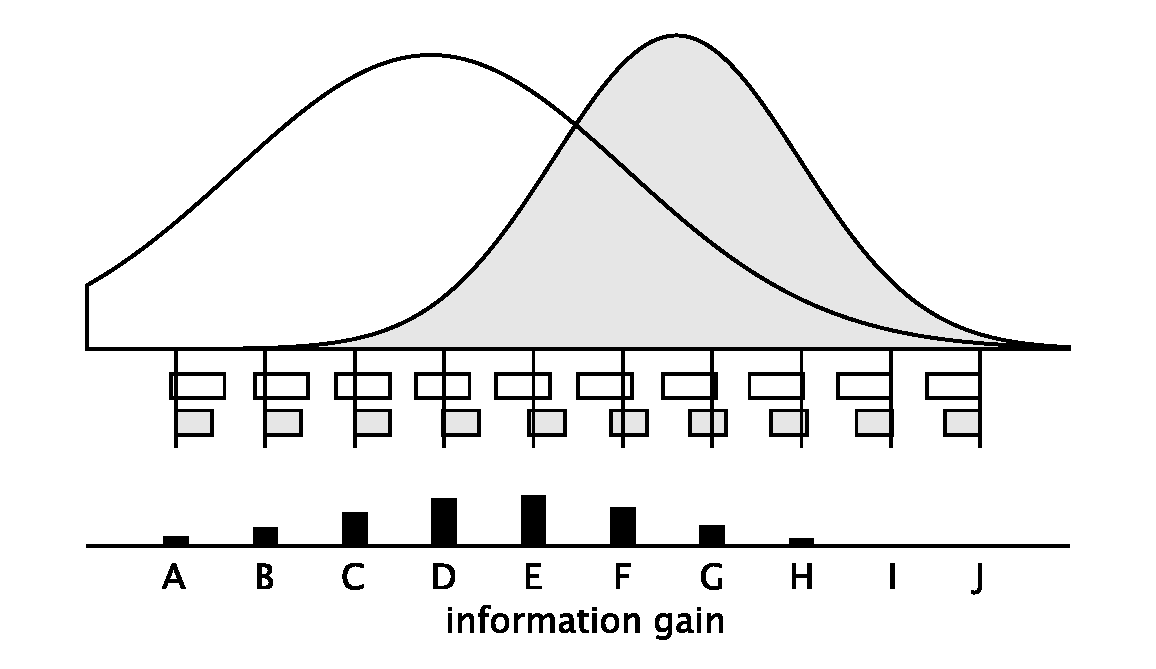
\includegraphics[width=\linewidth]{figures/gaussian2class}
\caption{Gaussian approximation of 2 classes.}
\label{fig:gaussian2class}
\end{figure}

\begin{figure}
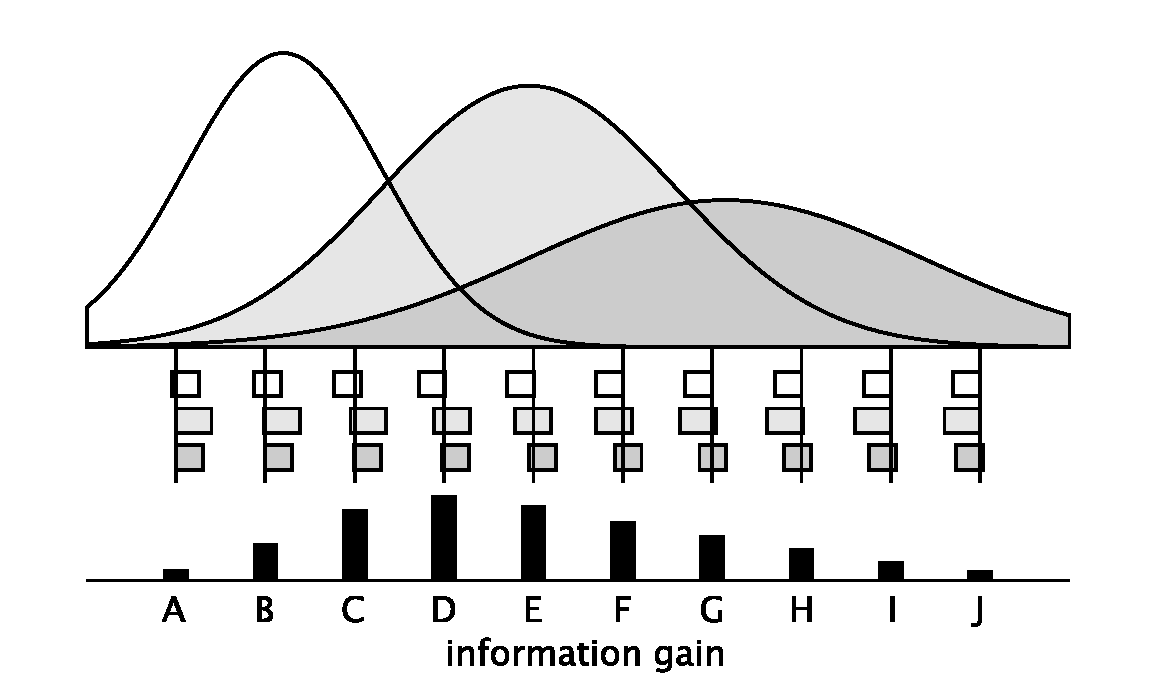
\includegraphics[width=\linewidth]{figures/gaussian3class}
\caption{Gaussian approximation of 3 classes.}
\label{fig:gaussian3class}
\end{figure}

\begin{figure}
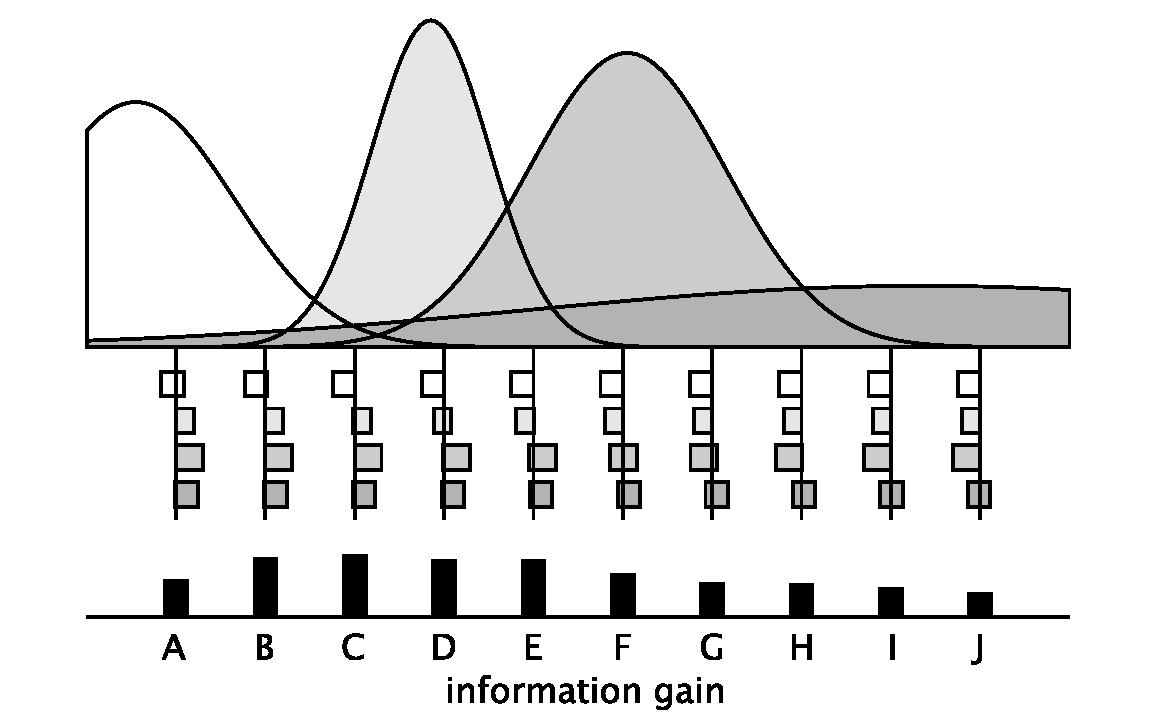
\includegraphics[width=\linewidth]{figures/gaussian4class}
\caption{Gaussian approximation of 4 classes.}
\label{fig:gaussian4class}
\end{figure}

The process is illustrated in Figures~\ref{fig:gaussian2class}-\ref{fig:gaussian4class}. At the top of each figure are Gaussian curves, each curve approximates the distribution of values seen for a numeric attribute and labeled with a particular class. The curves can be described using three values; the mean value, the standard deviation or variance of values, and the total weight of examples. For example, in Figure~\ref{fig:gaussian2class} the class shown to the left has a lower mean, higher variance and higher example weight (larger area under the curve) than the other class. Below the curves the range of values has been divided into ten split points, labeled A to J. The horizontal bars show the proportion of values that are estimated to lie on either side of each split, and the vertical bar at the bottom displays the relative amount of information gain calculated for each split. For the two-class example (Figure~\ref{fig:gaussian2class}), the split point that would be chosen as the best is point E, which according to the evaluation has the highest information gain. In the three-class example (Figure~\ref{fig:gaussian3class}) the preferred split point is point D. In the four-class example (Figure~\ref{fig:gaussian4class}) the split point C is chosen which nicely separates the first class from the others.

A refinement to this method, found to increase precision at low additional cost in early experiments, is used in the final implementation. It involves also tracking the minimum and maximum values of each class. This requires storing an extra two counts per class, but precisely maintaining these values is simple and fast. When evaluating split points the per-class minimum and maximum information is exploited to determine when class values lie completely to one side of a split, eliminating the small uncertainty otherwise present in the tails of the Gaussian curves. From the per-class minimum and maximum, the minimum and maximum of the entire range of values can be established, which helps to determine the position of split points to evaluate.

Intuitively it may seem that split points will only occur between the lowest and highest class mean, but this is not true. Consider searching for a split on the $age$ attribute of the {\sc genF1} data stream. The function is defined on page~\pageref{fig:agrawalFuncs1}, where the first class has $age$ values that are less than 40 and greater than 60, and the second class has $age$ values between 40 and 60. Obviously either 40 or 60 are the optimal split points, but the means of both class distributions will lie somewhere between 40 and 60---the first class will have a large variance estimate, and the second will be much narrower. This motivates searching across the entire range of values for a split. Using the absolute minimum and maximum value makes the procedure susceptible to outliers similar to the weakness of equal width discretization. A more robust search may instead consider each mean plus or minus several standard deviations to determine the potential splitting range. This possibility is reserved for future work.

Simple Gaussian approximation will almost certainly not capture the full detail of an intricate numeric distribution, but is highly efficient in both computation and memory. Where the binary tree method uses extreme memory costs to be as accurate as possible, this method employs the opposite approach---using gross approximation to use as little memory as possible.

%As is true with all of the approximate methods, this 
This simplified view of numeric distributions is not necessarily harmful to the accuracy of the trees it produces. There will be further opportunities to refine split decisions on a particular attribute by splitting again further down the tree.
%The method does not just have a single chance to get the optimal value but can have multiple attempts, 
All methods have multiple attempts at finding values,
where each subsequent attempt will be in a more focused range of values thus based on increasingly confident information.
The more approximate Gaussian method relies on this more than the less
approximate approaches. Also, the Gaussian approximation
%Also, the approximation
may prove more robust and resistant to noisy values than more complicated methods, which concentrate on finer details.

\subsection{Numerical Interval Pruning}
\label{sec:nip}

Another contribution is the work of Jin and Agrawal~\cite{nip} who present an approach called {\em numerical interval pruning} (NIP). The authors claim it is an efficient method ``which significantly reduces the processing time for numerical attributes, without loss in accuracy.'' Unfortunately insufficient details for reproducing the technique are provided in the paper. The numeric attribute range is divided into equal width intervals, and the intervals are then pruned if statistical tests determine that they are not likely to contain the best split point. Information is maintained in three ways---small class histograms, concise class histograms and detailed information (which can be in one of two formats, depending on which is most efficient). Without access to an actual implementation of their approach it is hard to be sure that any attempted reproduction of the technique, based on information provided in their paper, will be sufficiently faithful to the original. In their experimental evaluation, they found that the NIP method had more impact on computational cost than memory, in which they saw an average 39\% reduction in runtime compared to an exhaustive search for split points. Based on these findings, it should be possible to relate NIP performance to that of the binary tree. Judging by the reports, both methods are highly accurate, but in terms of memory NIP would be more efficient than the binary tree by a small amount. The experimental results show that even if a method is several times more space efficient than the exhaustive method it is still unlikely to compete with methods that use small and constant space per node.

\BEGINOMIT
\section{Experimental Comparison of Methods}
\label{sec:numexp}

The numeric summarization methods could be evaluated several ways, for example, the amount of error in each approximation could be directly measured for several sample distributions, and the computational and memory costs compared. While such a study may be interesting, it does not necessarily give an overall impression of how the methods work inside Hoeffding tree induction. So instead of studying small individual cases, the methods are tested to see how well they perform in the final role of interest---how efficiently they help to produce Hoeffding trees and how accurate the resulting trees are.

The experiment is conducted as previously set out in Chapter~\ref{chap:experimentalsetting}. Note that the {\sc led} data set is omitted from this analysis because it does not contain numeric attributes. The tree induction algorithm has the following properties, with only the method for handling numeric attributes varied:

\begin{itemize}
\item split confidence $\delta = 10^{-7}$ (Section~\ref{sec:splitconf})
\item grace period $n_{min} = 200$ (Section~\ref{sec:graceperiod})
\item pre-pruning {\em enabled} (Section~\ref{sec:preprune})
\item tie-breaking $\tau = 0.05$ (Section~\ref{sec:tiebreak})
\item skewed split prevention $p_{min} = 0.01$ (Section~\ref{sec:skewedsplits})
\item memory managed with {\em mem-period}=10,000 for 100KB environment, and {\em mem-period}=100,000 for 32MB/400MB environments (Section~\ref{sec:memmanage})
\item poor attribute removal {\em enabled} (Section~\ref{sec:pooratts})
\item majority class prediction (Section~\ref{sec:majclass})
\end{itemize}

These are the same basic settings used by {\sc htmc} in Chapter~\ref{chap:predstrat}. The numeric method employed will also affect the behaviour of {\em Naive Bayes} enhanced predictions described in Chapter~\ref{chap:predstrat}, which is avoided here by using majority class prediction to compare methods.

The numeric handling methods compared are listed in Table~\ref{tab:finalnummethods}, including the memory limits imposed per numeric attribute per leaf, and with reference to the text explaining each method.

\begin{table}
\caption{Final numeric methods compared.}
\label{tab:finalnummethods}
\centering
\begin{tabular}{|c|c|c|c|}
\hline
name & description & memory limit & section \\
\hline
\hline
{\sc vfml10} & VFML binning method & 10 bins & \ref{sec:vfmlnum} \\
\hline
{\sc vfml100} & VFML binning method & 100 bins & \ref{sec:vfmlnum} \\
\hline
{\sc vfml1000} & VFML binning method & 1000 bins & \ref{sec:vfmlnum} \\
\hline
{\sc bintree} & exhaustive binary tree & none & \ref{sec:bintreenum} \\
\hline
{\sc gk100} & Greenwald-Khanna & 100 tuples & \ref{sec:quantsum} \\
 & quantile summary & per class &  \\
 \hline
 {\sc gk1000} & Greenwald-Khanna & 1000 tuples & \ref{sec:quantsum} \\
 & quantile summary & per class &  \\
 \hline
{\sc gauss10} & Gaussian approximation & 5 values & \ref{sec:gaussapprox} \\
 & evaluating 10 split points & per class &  \\
 \hline
 {\sc gauss100} & Gaussian approximation & 5 values & \ref{sec:gaussapprox} \\
 & evaluating 100 split points & per class &  \\
\hline
\end{tabular}
\end{table}

Table~\ref{tab:numavgs} lists the final results averaged over all 18 data sources, sorted by memory-limited environment. Detailed results per data source are available in Appendix~\ref{sec:numericMethodTables}. 
The meaning of each column in the table is elaborated below:

\begin{description}
\item[accuracy] the percentage of examples that the tree was able to correctly predict from the one million examples reserved for testing
\item[training examples] the total number of examples that were used to train the tree before evaluation was complete
\item[active leaves] the number of active leaves in the tree (those that are capable of further splitting)
\item[inactive leaves] the number of leaves that have been deactivated by the memory management scheme (these are no longer capable of splitting)
\item[total nodes] the total number of nodes in the tree, including internal decision nodes
\item[tree depth] the depth of the tree---the length of the longest path from the root to a leaf
\item[training speed] the speed that the tree was able to train, expressed as a percentage of the maximum speed that examples can be generated from the data source, as measured in Section~\ref{sec:genspeed}
\item[prediction speed] the speed with which the tree could make predictions on the test data, again expressed as a percentage of maximum stream speed
\end{description}

The speeds achievable are quoted as percentages of the maximum speed that the streams can be generated by the experimental software/hardware. To complement the tables, Figures~\ref{fig:32MB_num1} and \ref{fig:32MB_num2} display learning curves for most problems in the 32MB/handheld environment, which contains the most interesting results of the three environments. The results for {\sc genF3} and {\sc genF10} are omitted from the figures because these graphs are the least interesting, showing little visible separation between methods.

\begin{table}
\caption{Final results averaged over all data sources comparing eight methods for handling numeric attributes.}
\label{tab:numavgs}
\centering
\begin{tabular}{|r|r|r|r|r|r|r|r|r|}
\hline
method	&
\rotatebox{90}{\parbox{9em}{accuracy\\(\%)}} &
\rotatebox{90}{\parbox{9em}{training examples\\(millions)}} &
\rotatebox{90}{\parbox{9em}{active leaves\\(hundreds)}} &
\rotatebox{90}{\parbox{9em}{inactive leaves\\(hundreds)}} &
\rotatebox{90}{\parbox{9em}{total nodes\\(hundreds)}} &
\rotatebox{90}{\parbox{9em}{tree depth}}	&
\rotatebox{90}{\parbox{9em}{training speed (\%)}} &
\rotatebox{90}{\parbox{9em}{prediction speed (\%)}} \\
\hline
\multicolumn{9}{|c|}{100KB memory limit / sensor} \\
\hline
{\sc vfml10} & 87.70 & 25 & 0 & 8.29 & 10.8 & 11 & 70 & 83 \\
{\sc vfml100} & 79.47 & 41 & 0 & 3.81 & 4.71 & 7 & 76 & 85 \\
{\sc vfml1000} & 76.06 & 1 & 0 & 0.09 & 0.14 & 3 & 81 & 88 \\
{\sc bintree} & 74.45 & 1 & 0 & 0.07 & 0.11 & 3 & 76 & 89 \\
{\sc gk100} & 82.92 & 29 & 0 & 4.31 & 5.35 & 9 & 71 & 84 \\
{\sc gk1000} & 74.65 & 1 & 0 & 0.08 & 0.13 & 3 & 59 & 88 \\
{\sc gauss10} & 86.16 & 27 & 0 & 8.96 & 12.2 & 12 & 69 & 81 \\
{\sc gauss100} & 85.33 & 28 & 0 & 8.33 & 11.9 & 20 & 64 & 79 \\
\hline
\multicolumn{9}{|c|}{32MB memory limit / handheld} \\
\hline
{\sc vfml10} & 91.53 & 901 & 31.8 & 674 & 1009 & 22 & 16 & 72 \\
{\sc vfml100} & 90.97 & 941 & 5.98 & 480 & 703 & 24 & 17 & 73 \\
{\sc vfml1000} & 90.97 & 952 & 4.28 & 412 & 604 & 27 & 17 & 73 \\
{\sc bintree} & 90.48 & 835 & 3.67 & 373 & 541 & 22 & 15 & 73 \\
{\sc gk100} & 89.96 & 962 & 6.88 & 531 & 777 & 34 & 17 & 73 \\
{\sc gk1000} & 90.94 & 961 & 2.70 & 403 & 581 & 27 & 16 & 75 \\
{\sc gauss10} & 91.35 & 892 & 94.8 & 683 & 1167 & 24 & 14 & 69 \\
{\sc gauss100} & 90.91 & 853 & 92.6 & 639 & 1167 & 50 & 14 & 65 \\
\hline
\multicolumn{9}{|c|}{400MB memory limit / server} \\
\hline
{\sc vfml10} & 91.41 & 293 & 320 & 80.4 & 591 & 24 & 4 & 73 \\
{\sc vfml100} & 91.19 & 142 & 73.9 & 143 & 316 & 23 & 4 & 74 \\
{\sc vfml1000} & 91.12 & 108 & 19.0 & 127 & 206 & 22 & 3 & 78 \\
{\sc bintree} & 90.50 & 60 & 13.7 & 92.9 & 147 & 19 & 2 & 80 \\
{\sc gk100} & 89.88 & 158 & 84.0 & 145 & 346 & 32 & 4 & 75 \\
{\sc gk1000} & 91.03 & 91 & 17.6 & 122 & 197 & 21 & 3 & 79 \\
{\sc gauss10} & 91.21 & 518 & 540 & 26.8 & 891 & 28 & 6 & 73 \\
{\sc gauss100} & 90.75 & 538 & 566 & 38.7 & 998 & 63 & 6 & 66 \\
\hline
\end{tabular}
\end{table}

Reviewing the average accuracies, the four different approaches are easily ranked from best to worst. In all three memory environments, {\sc vfml10} is the most accurate on average over all data sources. The second most accurate method in every environment is {\sc gauss10}. The {\sc gk}$x$ methods are generally third, and {\sc bintree} is consistently the least accurate of the methods on average.

The default number of 1000 bins hard-coded in the original {\sc vfml} implementation turns out to be the worst performer of the three {\sc vfml} configurations tested. The trend is that smaller approximations, in this case smaller numbers of bins, that sacrifice accuracy for space per leaf, lead to more accurate trees overall. Requesting more space for numeric approximation reduces the numbers of active tree nodes that can reside in memory, slowing tree growth in a way that harms final tree accuracy.

The Gaussian method follows this trend, in that it is the smallest approximation tested, translating into the fastest tree growth and correspondingly accurate trees. Comparing the number of split evaluations tested, it is apparent that the finer grained exploration of {\sc gauss100} can be harmful.
The {\sc gauss100} trees are on average much deeper than any of the other methods, suggesting that splits on certain numeric attributes are being repeated more often, because in many cases the tree depth exceeds the number of attributes available for splitting. These additional splits are probably very small and unnecessary refinements to previous split choices, and they may be very skewed. The skewed split parameter (Section~\ref{sec:skewedsplits}) aims to reduce spurious splitting, but in this case the default setting is not enough to prevent poor choices.
This is a symptom of trying to divide the range too finely based on approximation by a single smooth curve. The {\sc gauss10} method uses a suitably matched coarse division of only ten possibilities, which is far less susceptible to the same problem.

\begin{figure}
\centering
\begin{tabular}{c@{}c}
\includegraphics[width=0.5\textwidth]{figures/rts-r1-32MB_gkacc} &
\includegraphics[width=0.5\textwidth]{figures/rtc-r1-32MB_gkacc} \\
\end{tabular}
\caption{Examples of poor accuracy achieved by {\sc gk10} in 32MB.}
\label{fig:gk10}
\end{figure}

Comparing the quantile summary methods {\sc gk100} and {\sc gk1000}, having 1000 tuples is helpful in the higher memory environments but harmful in 100KB of memory. Lower numbers of tuples can severely hinder the quantile summary method---a parameter setting of ten was tested but found to be much worse than any other method, so is omitted from the final results. Figure~\ref{fig:gk10} shows some examples of how much worse the ten-tuple summary can perform. In particular, the graph on {\sc rts} shows other settings getting very close to 100\% accuracy in contrast to the ten-tuple variant achieving less than 65\%. Like {\sc gauss100}, {\sc gk10} suffers from symptoms of excessively deep trees which strongly indicates poor numeric split decisions. Larger quantile summaries perform well but the tradeoff between space and accuracy is not as effective as for the {\sc gauss}$x$ and {\sc vfml}$x$ methods. The performance of {\sc gk1000} is similar to {\sc bintree} in several situations, suggesting that it is highly accurate, while at the same time it manages to build larger trees, suggesting that it is more space efficient than {\sc bintree}.

The poor performance of {\sc bintree} shows that in limited memory situations, striving for perfect accuracy at the local level can result in lower accuracy globally. The problem is most pronounced in the 100KB sensor network environment, where tree growth for every data source was halted before the first evaluation took place, some time before one million training examples. 
Similar behaviour is evident in the other two most memory-intensive methods {\sc vfml1000} and {\sc gk1000}, but {\sc bintree} has the highest memory requirements of all, thus suffers the most in tree growth and accuracy.
The method is simply too memory-hungry to support reasonable tree induction in this environment. In the other environments it fares better, but is not as successful on average as the more approximate methods.

\begin{table}
\caption{{\sc vfml10} vs {\sc gauss10} accuracy (\%).}
\label{tab:vfml10_vs_gauss10_acc}
\centering
\begin{tabular}{|r||r|r|r||r|r|r|}
\hline
method$\rightarrow$ & \multicolumn{3}{|c||}{{\sc vfml10}} & \multicolumn{3}{|c|}{{\sc gauss10}} \\
\hline
 & \multicolumn{3}{|c||}{memory limit} & \multicolumn{3}{|c|}{memory limit} \\
\hline
dataset & 100KB & 32MB & 400MB & 100KB & 32MB & 400MB \\
\hline
{\sc rts} & 96.49 & 99.99 & 99.98 & \textbf{96.95} & 99.99 & \textbf{99.99} \\
{\sc rtsn} & \textbf{75.80} & \textbf{78.54} & \textbf{78.53} & 75.20 & 78.48 & 78.45 \\
{\sc rtc} & 61.37 & \textbf{83.58} & \textbf{83.87} & \textbf{62.49} & 83.00 & 83.02 \\
{\sc rtcn} & 53.63 & \textbf{64.95} & \textbf{66.06} & 53.63 & 62.45 & 61.87 \\
{\sc rrbfs} & 87.69 & 93.13 & 92.43 & \textbf{88.56} & \textbf{93.27} & \textbf{92.93} \\
{\sc rrbfc} & 87.84 & 98.61 & 97.41 & \textbf{91.36} & \textbf{98.72} & \textbf{98.21} \\
{\sc wave21} & 80.80 & 84.20 & 83.50 & \textbf{81.21} & \textbf{84.37} & \textbf{84.01} \\
{\sc wave40} & 80.28 & 84.00 & 83.31 & \textbf{81.20} & \textbf{84.21} & \textbf{83.80} \\
{\sc genF1} & 95.07 & 95.07 & 95.07 & 95.07 & 95.07 & 95.07 \\
{\sc genF2} & \textbf{93.94} & \textbf{94.10} & \textbf{94.10} & 78.46 & 94.03 & 94.00 \\
{\sc genF3} & \textbf{97.52} & 97.52 & 97.52 & 97.50 & 97.52 & 97.52 \\
{\sc genF4} & \textbf{94.46} & 94.67 & \textbf{94.66} & 93.68 & 94.67 & 94.65 \\
{\sc genF5} & \textbf{92.45} & \textbf{92.89} & \textbf{92.84} & 71.73 & 92.36 & 92.15 \\
{\sc genF6} & 89.70 & \textbf{93.35} & 93.28 & \textbf{91.89} & 93.31 & 93.28 \\
{\sc genF7} & 96.41 & \textbf{96.82} & 96.79 & \textbf{96.51} & 96.81 & 96.79 \\
{\sc genF8} & 99.40 & 99.42 & 99.42 & \textbf{99.41} & 99.42 & 99.42 \\
{\sc genF9} & 95.80 & \textbf{96.81} & 96.72 & \textbf{96.07} & 96.78 & \textbf{96.74} \\
{\sc genF10} & \textbf{99.89} & 99.89 & 99.89 & 99.88 & 99.89 & 99.89 \\
\hline
average & 87.70 & 91.53 & 91.41 & 86.16 & 91.35 & 91.21 \\
\hline
\end{tabular}
\end{table}

\begin{figure}
\centering
\begin{tabular}{c@{}c}
\includegraphics[width=0.5\textwidth]{figures/rts-r1-32MB_numaccuracy} &
\includegraphics[width=0.5\textwidth]{figures/rtsn-r1-32MB_numaccuracy} \\
\includegraphics[width=0.5\textwidth]{figures/rtc-r1-32MB_numaccuracy} &
\includegraphics[width=0.5\textwidth]{figures/rtcn-r1-32MB_numaccuracy} \\
\includegraphics[width=0.5\textwidth]{figures/rrbfs-r1-32MB_numaccuracy} &
\includegraphics[width=0.5\textwidth]{figures/rrbfc-r1-32MB_numaccuracy} \\
\includegraphics[width=0.5\textwidth]{figures/wave21-r1-32MB_numaccuracy} &
\includegraphics[width=0.5\textwidth]{figures/wave40-r1-32MB_numaccuracy} \\
\end{tabular}
\caption{Part 1 of learning curves for numeric methods in 32MB memory limit.}
\label{fig:32MB_num1}
\end{figure}

\begin{figure}
\centering
\begin{tabular}{c@{}c}
\includegraphics[width=0.5\textwidth]{figures/genF1-r1-32MB_numaccuracy} &
\includegraphics[width=0.5\textwidth]{figures/genF2-r1-32MB_numaccuracy} \\
\includegraphics[width=0.5\textwidth]{figures/genF4-r1-32MB_numaccuracy} &
\includegraphics[width=0.5\textwidth]{figures/genF5-r1-32MB_numaccuracy} \\
\includegraphics[width=0.5\textwidth]{figures/genF6-r1-32MB_numaccuracy} &
\includegraphics[width=0.5\textwidth]{figures/genF7-r1-32MB_numaccuracy} \\
\includegraphics[width=0.5\textwidth]{figures/genF8-r1-32MB_numaccuracy} &
\includegraphics[width=0.5\textwidth]{figures/genF9-r1-32MB_numaccuracy} \\
\end{tabular}
\caption{Part 2 of learning curves for numeric methods in 32MB memory limit.}
\label{fig:32MB_num2}
\end{figure}

Table~\ref{tab:vfml10_vs_gauss10_acc} compares the individual final accuracies of the best two methods, {\sc vfml10} and {\sc gauss10}. Bold figures indicate a better result, in this case both methods win 20 times each.
{\sc gauss10} loses to {\sc vfml10} by a wide margin on {\sc rtcn} in 400MB, although on this data set some of the other methods are not much better than {\sc gauss10} and some are worse still.
Some of the worst losses for {\sc gauss10} occur on {\sc genF2} and {\sc genF5} in 100KB, where it is outperformed by all other methods. Referring back to the functions generating the underlying concept of these data streams (Figure~\ref{fig:agrawalFuncs1}, page~\pageref{fig:agrawalFuncs1}), these functions are very similar. The function of {\sc genF2} relies on the two numeric attributes $salary$ and $age$, and {\sc genF5} adds another layer of complexity by including dependency on a third numeric attribute, $loan$. From an inspection of the learning curves at the top right of Figure~\ref{fig:32MB_num2} it is clear that the Gaussian methods struggle with these concepts more than any of the other methods.
The trees induced by the Gaussian method were inspected to find the cause of the problem. In this case the trees make the mistake of choosing a discrete attribute with many possible values that is completely irrelevant, $car$. After making this mistake the example space is highly segmented, so a lot of extra effort is required to correct the mistake further down the tree. The Gaussian methods slowly recover to come within reasonably close accuracy, besides the 100KB environment where the differences are exaggerated due to lack of space limiting opportunity to recover. This demonstrates a limitation of the Gaussian method, where the high level of approximation causes the best attributes to be underrated, although the true underlying cause of the issue is unknown, perhaps relating to an unintentional bias towards certain split types that could potentially be corrected in similar style to Quinlan's correction in~\cite{c4.5rel8}. This is reserved for future work.

Conversely, there are situations where the high level of approximation gives the Gaussian method an advantage over all others. The clearest cases of this are on the data sources {\sc rrbfs}, {\sc rrbfc}, {\sc wave21} and {\sc wave40}.
Such a bias may not be surprising when the generators responsible for these streams use numeric values drawn from random Gaussian distributions.

Analysing space complexity, the amount of memory required per leaf to track $n$ numeric attributes and $c$ classes is $10n+10nc$ for {\sc vfml10} and $5nc$ for {\sc gauss10}. For {\sc vfml10} the $10n$ term accounts for storage of the boundary positions, while the $10nc$ term accounts for the frequency counts. This simplified analysis underestimates the true cost of the {\sc vfml} implementation, which also retains information about the class and frequency of values that lie exactly on the lower boundary of each bin, increasing the precision of decisions. For {\sc gauss10} the multiplying constant is five values per attribute and class because there are three values tracking the Gaussian curve and and additional two numbers tracking the minimum and maximum values. Clearly {\sc gauss10} requires the least memory.

\begin{figure}
\centering
\begin{tabular}{c@{}c}
\includegraphics[width=0.5\textwidth]{figures/vfml_vs_gauss_unsorted} &
\includegraphics[width=0.5\textwidth]{figures/vfml_vs_gauss_sorted} \\
\end{tabular}
\caption{Effect that example ordering has on learning accuracy in 32MB on the {\sc genF2} data. Left hand side: default random order. Right hand side: modified stream where every consecutive sequence of one million training examples has been sorted on the value of the $salary$ attribute.}
\label{fig:genf2sorted}
\end{figure}

In theory, at the local level {\sc vfml10} should be very sensitive to data order, whereas {\sc gauss10} should not be sensitive at all. Whether this can translate into poorer global decisions during tree induction is not tested by the benchmark generators because all examples are randomly drawn somewhat uniformly from the space of possible examples. The right hand side of Figure~\ref{fig:genf2sorted} shows a constructed example where data order has been manipulated to expose {\sc vfml10}'s weakness. {\sc genF2} has been modified so that every sequence of one million examples drawn from the stream has been sorted by the $salary$ attribute.
In this case the accuracy of {\sc gauss10} has improved while the early accuracy of {\sc vfml10} has dropped markedly.
The ability of {\sc vfml10} to slowly recover may be partly due to additional tree structure increasing the dispersion of examples down different paths of the tree, reducing the degree to which values encountered at leaves are sorted.

The {\sc gauss10} method is highly competitive on most data sets besides being outperformed by {\sc vfml10} in a few cases. It uses less memory than {\sc vfml10} and is less susceptible to data order.
For these reasons {\sc gauss10} is used as the default numeric handling method for the remainder of the \thesisc, used in the {\sc htmc} method of Section~\ref{sec:leafexp}. Even though {\sc htmc} and {\sc gauss10} refer to the same algorithm they are kept separate for comparison purposes because the numeric experiments exclude the {\sc led} data source, causing the average of reported accuracies to differ.

On average, {\sc gauss10} trees reach much larger sizes than the other numeric methods in the same time and space, with many more active leaves. The lack of information during local decisions is made up for by increased tree structure, leading to trees that are more accurate overall. The general conclusion of this study of numeric handling techniques is that the most accurate methods for data streams  are those that use very little space, but make up for loss of local accuracy by enabling tree growth to be much more productive. 

\section{Summary}

This chapter studied the difficult challenge of managing continuous numeric attributes in data streams for the purposes of inducing decision trees. Five main approaches from the literature were discussed, and eight final configurations of algorithm were tested, ranging from perfectly accurate and memory intensive to highly approximate and lightweight. In experimental comparison, the most lightweight methods produced the most accurate trees, by virtue of being the lowest impediment to tree growth. The smallest approximation of all, the {\sc gauss10} method, was selected as the default numeric handling technique for the rest of the \thesisc. It is based on simple Gaussian approximation, similar to the method suggested by Gama et al.~\cite{ufft} but selects split points in a way that accommodates multiple class labels.

Before this investigation, {\sc vfml1000} was considered the default
numeric handling strategy, as it is the strategy used by the public
implementation of VFDT~\cite{vfml}. Averaged over all data sets and
environments, and including accuracy on {\sc led} for consistency with the
studies that follow, the accuracy of {\sc vfml1000} is 85.41\%. The accuracy
of {\sc gauss10}, which will be referred to as {\sc htmc} in
the next chapter, is 88.75\%. The relative average improvement in accuracy,
gained by selecting a more efficient numeric handling method, is 3.91\%. This comes with an overall average training speed reduction of 11.88\%, and an average prediction speed reduction of 6.75\%.

Most of the accuracy gains were in the 100KB environment with a relative gain of 12.59\%. In this environment training and prediction speed reduced by 13.75\% and 7.95\% respectively. In 32MB the relative accuracy gain was 0.41\%, with training and prediction speed reducing by 17.65\% and 4.17\%. In 400MB where more expensive methods were able to compete better, the relative accuracy gain was only 0.10\% on average. The training speed actually increased by half in this environment, while the prediction speed reduced by 7.79\%.
\ENDOMIT %\cleardoublepage{}
\chapter{Prediction Strategies}
\label{chap:predstrat} 

The previous chapters have considered the induction of Hoeffding trees.
Chapter~\ref{chap:hoeffdingtrees} covered the basic induction of Hoeffding trees, followed by Chapter~\ref{chap:numericatts} which investigated the handling of continuous numeric attributes in the training data. This chapter focuses on the use of models once they have been induced---how predictions are made by the trees. Section~\ref{sec:majclass} describes the standard {\em majority class} prediction method. Attempts to outperform this method are described in Section~\ref{sec:nbleaf} and \ref{sec:nbadaptive}. %The chapter concludes with an experiment in Section~\ref{sec:leafexp} to determine which method is best in practice.

\section{Majority Class}
\label{sec:majclass}

Prediction using decision trees is straightforward. Examples with unknown label are filtered down the tree to a leaf, and the most likely class label retrieved from the leaf. An obvious and straightforward way of assigning labels to leaves is to determine the most frequent class of examples that were observed there during training. This method is used by the batch methods C4.5/CART and is naturally replicated in the stream setting by Hoeffding trees. If the likelihood of all class labels is desired, an immediate extension is to return a probability distribution of class labels, once again based on the distribution of classes observed from the training examples.

Table~\ref{tab:leafsuffstats} is used to illustrate different prediction schemes throughout the chapter. In the case of majority class, the leaf will always predict class $C_{2}$ for every example, because most examples seen before have been of that class. There have been 60 examples of class $C_{2}$ versus 40 examples of class $C_{1}$, so the leaf will estimate for examples with unknown class that the probability of class $C_{2}$ is 0.6, and the probability of $C_{1}$ is 0.4.

\begin{table}
\caption{Example sufficient statistics in a leaf after 100 examples have been seen. There are two class labels: $C_{1}$ has been seen 40 times, and $C_{2}$ has been seen 60 times. There are three attributes: $A_{1}$ can either have value A or B, $A_{2}$ can be C, D or E, and $A_{3}$ can be F, G, H or I. The values in the table track how many times each of the values have been seen for each class label.}
\label{tab:leafsuffstats}
\centering
\begin{tabular}{|c|c||c|c|c||c|c|c|c||c|c|}
\hline
\multicolumn{2}{|c||}{$A_{1}$} & \multicolumn{3}{|c||}{$A_{2}$} & \multicolumn{4}{|c||}{$A_{3}$} & & \\
\hline
A & B & C & D & E & F & G & H & I & class & total \\
\hline
12 & 28 & 5 & 10 & 25 & 13 & 9 & 3 & 15 & $C_{1}$ & 40 \\
34 & 26 & 21 & 8 & 31 & 11 & 21 & 19 & 9 & $C_{2}$ & 60 \\
\hline
\end{tabular}
\end{table}

\section{Naive Bayes Leaves}
\label{sec:nbleaf}

There is more information available during prediction in the leaves of a Hoeffding tree than is considered using majority class classification. The attribute values determine the path of each example down the tree, but once the appropriate leaf has been established it is possible to use the same attribute values to further refine the classification. Gama et al. call this enhancement {\em functional tree leaves}~\cite{ufft,vfdtc}.

If $P(C)$ is the probability of event $C$ occurring, and $P(C|X)$ is the probability of event $C$ given that $X$ occurs, then from Bayes' theorem:

\begin{equation} \label{eq:bayes}
P(C|X) = \frac{P(X|C) P(C)}{P(X)}
\end{equation}

This rule is the foundation of the Naive Bayes classifier~\cite{naivebayes}. The classifier is called `naive' because it assumes independence of the attributes. The independence assumption means that for each example the value of any attribute will not have a bearing on the value of any other attribute. It is not realistic to expect such simplistic attribute relationships to be common in practice, but despite this the classifier works surprisingly well in general~\cite{nboptimal,nbdiagnose}.

By collecting the probabilities of each attribute value with respect to the class label from training examples, the probability of the class for unlabeled examples can be computed. Fortunately, the sufficient statistics being maintained in leaves of a Hoeffding tree for the purpose of choosing split tests are also the statistics required to perform Naive Bayes classification. 

Returning to the example in Table~\ref{tab:leafsuffstats}, if an example being classified by the leaf has attribute values $A_{1}$=B, $A_{2}$=E and $A_{3}$=I then the likelihood of the class labels is calculated using Equation~\ref{eq:bayes}:
\begin{eqnarray*}
P(C_{1}|X) & = & \frac{ P(X|C_{1}) P(C_{1})}{P(X)} \\
& = & \frac{ [P(B|C_{1}) \times P(E|C_{1}) \times P(I|C_{1})] \times P(C_{1})}{P(X)} \\
& = & \frac{\frac{28}{40} \times \frac{25}{40} \times \frac{15}{40} \times \frac{40}{100}}{P(X)} \\
& = & \frac{0.065625}{P(X)}
\end{eqnarray*}
\begin{eqnarray*}
P(C_{2}|X) & = & \frac{ P(X|C_{2}) P(C_{2})}{P(X)} \\
& = & \frac{ [P(B|C_{2}) \times P(E|C_{2}) \times P(I|C_{2})] \times P(C_{2})}{P(X)} \\
& = & \frac{\frac{26}{60} \times \frac{31}{60} \times \frac{9}{60} \times \frac{60}{100}}{P(X)} \\
& = & \frac{0.02015}{P(X)}
\end{eqnarray*}
Normalizing the likelihoods means that the common $P(X)$ denominator is eliminated to reach the final probabilities:
\begin{displaymath}
\mbox{probability of } C_{1} = \frac{0.065625}{0.065625 + 0.02015} = 0.77
\end{displaymath}
\begin{displaymath}
\mbox{probability of } C_{2} = \frac{0.02015}{0.065625 + 0.02015} = 0.23
\end{displaymath}
So in this case the Naive Bayes prediction chooses class $C_{1}$, contrary to the majority class.

A technicality omitted from the example is the {\em zero frequency} problem that occurs if one of the counts in the table is zero. The Naive Bayes calculation cannot be performed with a probability of zero, so the final implementation overcomes this by using a {\em Laplace} estimator of  1.
This adjustment, based on {\em Laplace's Law of Succession}, means for example that the class prior probabilities in the example above are instead treated as $\frac{41}{102}$ and $\frac{61}{102}$.

In batch learning the combination of decision trees and Naive Bayes classification has been explored by Kohavi in his work on {\em NBTrees}~\cite{nbtree}. Kohavi's NBTrees are induced by specifically choosing tests that give an accuracy advantage to Naive Bayes leaves. In that setting he found that the hybrid trees could often outperform both single decision trees and single Naive Bayes models. He noted that the method performs well on large data sets, although the meaning of large in the batch setting can differ greatly from the modern stream context---most of the training sets he tested had less than 1,000 examples, with the largest set having under 50,000 examples.

Use of Naive Bayes models in Hoeffding tree induction has implications for the memory management strategy. Firstly, the act of deactivating leaf nodes is more significant, because throwing away the sufficient statistics will also eliminate a leaf's ability to make a Naive Bayes prediction. The heuristic used to select the most promising nodes does not take this into account, as it does not consider the possibility that a leaf may be capable of yielding better accuracy than majority class. For simplicity and consistency in the experimental implementation, the memory management strategy is not changed when Naive Bayes leaves are enabled. This makes sense if the use of Naive Bayes leaves are considered as a prediction-time enhancement to Hoeffding trees. Otherwise changes to memory management behaviour intended to better suit Naive Bayes prediction will significantly impact on overall tree induction, making it harder to interpret direct comparisons with majority class trees.

The outcome of this approach is that when memory gets tight and fewer of the leaves are allowed to remain active, then fewer of the leaves will be capable of Naive Bayes prediction. The fewer the active leaves, the closer the tree will behave to a tree that uses majority class only. By the time the tree is frozen and can no longer afford to hold any active leaves in memory then the tree will have completely reverted to majority class prediction. This behaviour is noted when looking at the experimental results.

The other issue is the secondary memory management strategy of removing poor attributes (Section~\ref{sec:pooratts}). This too will alter the effectiveness of Naive Bayes models, because removing information about attributes removes some of the power that the Naive Bayes models use to predict, regardless of whether the attributes are deemed a poor candidate for splitting or not. As the removal strategy has been shown to not have a large bearing on final tree accuracy, whenever Naive Bayes leaves are employed the attribute removal strategy is not used.

Memory management issues aside, the Naive Bayes enhancement adds no cost to the induction of a Hoeffding tree, neither to the training speed nor memory usage. All of the extra work is done at prediction time. The amount of prediction-time overhead is quantified in the experimental comparison.

Early experimental work confirmed that Naive Bayes predictions are capable of increasing accuracy as Gama et al. observed~\cite{ufft,vfdtc}, but also exposed cases where Naive Bayes prediction fares worse than majority class. The first response to this problem was to suspect that some of the leaf models are immature. In the early stages of a leaf's development the probabilities estimated may be unreliable because they are based on very few observations. If that is the case then there are two possible remedies; either (1) give them a jump-start to make them more reliable from the beginning, or (2) wait until the models are more reliable before using them.

Previous work~\cite{stresstest} has covered several attempts at option (1) of `priming' new leaves with better information. One such attempt, suggested by Gama et al.~\cite{ufft} is to remember a limited number of the most recent examples from the stream, for the purposes of training new leaves as soon as they are created. A problem with this idea is that the number of examples able to be retrieved that apply to a particular leaf will diminish as the tree gets progressively deeper. Other attempts at priming involved trying to inject more of the information known prior to splitting into the resulting leaves of the split. Neither of these attempts were successful at overcoming the problem so are omitted from consideration.

%The experimental results in Section~\ref{sec:leafexp} test two variations of option (2), waiting before trusting Naive Bayes models. The first is very simple---a fixed minimum number of examples are required at a leaf before Naive Bayes prediction is employed. The higher the threshold, the longer the tree will wait and the more often majority class prediction will be used. Setting it too high will not see any change from exclusive use of majority class, and setting it too low will permit premature use of Naive Bayes. The threshold used in the presented results is one thousand examples, which is not overly successful at solving the problem but was found in preliminary experimentation to be the best compromise.

%It appears that a single fixed threshold is simply not sufficient to overcome the problem, motivating further exploration of methods. This led to the development and contribution of a second more sophisticated waiting strategy discussed next.

\section{Adaptive Hybrid}
\label{sec:nbadaptive}

Cases where Naive Bayes decisions are less accurate than majority class are a concern because more effort is being put in to improve predictions and instead the opposite occurs. In those cases it is better to use the standard majority class method, making it harder to recommend the use of Naive Bayes leaf predictions in all situations.

The method described here tries to make the use of Naive Bayes models more reliable, by only trusting them on a per-leaf basis when there is evidence that there is a true gain to be made.
The {\em adaptive} method works by monitoring the error rate of majority class and Naive Bayes decisions in every leaf, and choosing to employ Naive Bayes decisions only where they have been more accurate in past cases. Unlike pure Naive Bayes prediction, this process {\em does} introduce an overhead during training. Extra time is spent per training example generating both prediction types and updating error estimates, and extra space per leaf is required for storing the estimates.

\begin{algorithm}
\caption{Adaptive prediction algorithm.}
\begin{algorithmic}
\FORALL{training examples}
\STATE Sort example into leaf $l$ using $HT$
\IF{$majorityClass_{l} \ne$ true class of example}
\STATE increment $mcError_{l}$
\ENDIF
\IF{$NaiveBayesPrediction_{l}$(example) $\ne$ true class of example}
\STATE increment $nbError_{l}$
\ENDIF
\STATE Update sufficient statistics in $l$
\STATE ...
\ENDFOR
\STATE
\FORALL{examples requiring label prediction}
\STATE Sort example into leaf $l$ using $HT$
\IF{$nbError_{l} < mcError_{l}$}
\RETURN $NaiveBayesPrediction_{l}$(example)
\ELSE
\RETURN $majorityClass_{l}$
\ENDIF
\ENDFOR
\end{algorithmic}
\label{alg:htnba}
\end{algorithm}


The pseudo-code listed in Algorithm~\ref{alg:htnba} makes the process explicit. During training, once an example is filtered to a leaf but before the leaf is updated, both majority class prediction and Naive Bayes prediction are performed and both are compared with the true class of the example. Counters are incremented in the leaf to reflect how many errors the respective methods have made. At prediction time, a leaf will use majority class prediction unless the counters suggest that Naive Bayes prediction has made fewer errors, in which case Naive Bayes prediction is used instead.

In terms of the example in Table~\ref{tab:leafsuffstats}, the class predicted for new examples will depend on extra information. If previous training examples were more accurately classified by majority class than Naive Bayes then class $C_{2}$ will be returned, otherwise the attribute values will aid in Naive Bayes prediction as described in the previous subsection.

\BEGINOMIT
The accuracy gains afforded by this method and the extra costs involved are empirically quantified next.


\section{Experimental Comparison of Methods}
\label{sec:leafexp}

This section uses the testing framework established in Chapter~\ref{chap:experimentalsetting} to compare four strategies for Hoeffding tree prediction. To ease reference to these methods in the text, each has been assigned a short name---the methods are called {\sc htmc}, {\sc htnb}, {\sc htnb1k} and {\sc htnba}. Several elements to Hoeffding tree induction have been covered previously, so the following list summarizes the final properties of each method including references to explanatory text:

\begin{enumerate}
\item {\sc htmc} algorithm, properties:
\begin{itemize}
\item split confidence $\delta = 10^{-7}$ (Section~\ref{sec:splitconf})
\item grace period $n_{min} = 200$ (Section~\ref{sec:graceperiod})
\item pre-pruning {\em enabled} (Section~\ref{sec:preprune})
\item tie-breaking $\tau = 0.05$ (Section~\ref{sec:tiebreak})
\item skewed split prevention $p_{min} = 0.01$ (Section~\ref{sec:skewedsplits})
\item memory managed with {\em mem-period}=10,000 for 100KB environment, and {\em mem-period}=100,000 for 32MB/400MB environments \\ (Section~\ref{sec:memmanage})
\item poor attribute removal {\em enabled} (Section~\ref{sec:pooratts})
\item numeric attributes handled with {\em Gaussian approximation} using 10 split evaluations (Section~\ref{sec:gaussapprox})
\item majority class prediction (Section~\ref{sec:majclass})
\end{itemize}
\item {\sc htnb} algorithm, properties that differ from {\sc htmc}:
\begin{itemize}
\item poor attribute removal {\em disabled} (Section~\ref{sec:pooratts} and~\ref{sec:nbleaf})
\item Naive Bayes prediction (Section~\ref{sec:nbleaf})
\end{itemize}
\item {\sc htnb1k} algorithm, properties that differ from {\sc htnb}:
\begin{itemize}
\item majority class prediction in each leaf until 1000 examples seen, then Naive Bayes prediction afterwards (Section~\ref{sec:nbleaf})
\end{itemize}
\item {\sc htnba} algorithm, properties that differ from {\sc htnb}:
\begin{itemize}
\item adaptive hybrid majority class/Naive Bayes prediction decided per leaf (Section~\ref{sec:nbadaptive})
\end{itemize}
\end{enumerate}

{\sc htmc} is a re-implementation that for the most part is equivalent to the VFDT system, and as such can be considered the base Hoeffding tree method. Following the findings from the previous chapter, numeric attributes are handled using a Gaussian approximation that evaluates ten split points.
In the current comparison the modifications tested involve changing the prediction strategies used by the tree, with {\sc htmc} representing the default majority class method.

\begin{table}
\caption{Final results averaged over all data sources comparing four methods for Hoeffding tree prediction.}
\label{tab:leafavgs}
\centering
\begin{tabular}{|r|r|r|r|r|r|r|r|r|}
\hline
method	&
\rotatebox{90}{\parbox{9em}{accuracy\\(\%)}} &
\rotatebox{90}{\parbox{9em}{training examples\\(millions)}} &
\rotatebox{90}{\parbox{9em}{active leaves\\(hundreds)}} &
\rotatebox{90}{\parbox{9em}{inactive leaves\\(hundreds)}} &
\rotatebox{90}{\parbox{9em}{total nodes\\(hundreds)}} &
\rotatebox{90}{\parbox{9em}{tree depth}}	&
\rotatebox{90}{\parbox{9em}{training speed (\%)}} &
\rotatebox{90}{\parbox{9em}{prediction speed (\%)}} \\
\hline
\multicolumn{9}{|c|}{100KB memory limit / sensor} \\
\hline
{\sc htmc} & 85.51 & 27 & 0 & 8.64 & 11.9 & 12 & 69 & 81 \\
{\sc htnb} & 85.48 & 27 & 0 & 8.69 & 11.9 & 12 & 68 & 81 \\
{\sc htnb1K} & 85.48 & 27 & 0 & 8.69 & 11.9 & 12 & 68 & 81 \\
{\sc htnba} & 85.44 & 29 & 0 & 8.65 & 11.9 & 12 & 67 & 82 \\
\hline
\multicolumn{9}{|c|}{32MB memory limit / handheld} \\
\hline
{\sc htmc} & 90.44 & 902 & 92.3 & 659 & 1134 & 24 & 14 & 69 \\
{\sc htnb} & 90.48 & 825 & 75.1 & 643 & 1063 & 24 & 14 & 63 \\
{\sc htnb1K} & 90.48 & 905 & 72.5 & 691 & 1136 & 24 & 14 & 63 \\
{\sc htnba} & 90.51 & 871 & 73.4 & 670 & 1106 & 24 & 14 & 65 \\
\hline
\multicolumn{9}{|c|}{400MB memory limit / server} \\
\hline
{\sc htmc} & 90.30 & 525 & 522 & 25.4 & 864 & 28 & 6 & 71 \\
{\sc htnb} & 90.24 & 464 & 471 & 49.1 & 802 & 28 & 6 & 40 \\
{\sc htnb1K} & 90.34 & 450 & 494 & 49.1 & 847 & 28 & 6 & 42 \\
{\sc htnba} & 90.70 & 463 & 489 & 46.7 & 828 & 28 & 6 & 53 \\
\hline
\end{tabular}
\end{table}

Table~\ref{tab:leafavgs} summarizes behaviour of the four methods for each of the three environments. The numbers have been averaged over all data sources. For a more detailed breakdown of the results per data source refer to the tables in Appendix~\ref{sec:predictionMethodTables}.

Recall from Chapter~\ref{chap:experimentalsetting} that each method is allowed a total of ten hours training time. The results reported in the tables represent the final result recorded when ten hours of training were complete or earlier if the tree became frozen. Excessive evaluation overhead was avoided by only measuring and recording the properties of the trees after every ten million training examples in the 32MB/400MB environments, and more frequently in the 100KB environment where changes happen more rapidly, every one million examples.

First, looking at the properties of the trees besides accuracy, it is clear that the 100KB sensor environment strongly limits what the algorithms can achieve.
In this environment fewer training examples are processed than possible in higher memory environments.
This happened on every data set, and was caused by tree growth halting after all leaves have been deactivated well before the ten hour training limit.
In fact, the training times in 100KB did not exceed 30 minutes in any run.
Because the final trees have been stripped of their active nodes they are effectively only capable of majority class prediction. This explains why the prediction speeds attained by the final trees hardly differ between prediction methods in this environment. One positive effect that the highly constrained memory limit has compared to the other environments is that it allows much higher training speeds to be attained, but this provides little consolation when only limited training is possible.

Looking at environments with higher memory, differences between the four methods begin to show and are the most pronounced in the server environment. It is interesting to see that the server environment is not capable of processing as many examples in the ten hour period as the 32MB handheld environment, neither is it able to grow as many nodes. This can be explained by looking at the extra amount of work involved in maintaining the trees in the largest memory environment. The trees are deeper and have many more active leaves to evaluate, slowing computation and limiting the number of examples that can be handled in a given time.

The average training speed is not significantly affected by the prediction method utilized, which is to be expected in the first three methods as they do not alter the amount of work performed during training, but this is a very positive sign for {\sc htnba} which does in fact do some extra computation per training example. An explanation for this is that the extra processing is integrated with the induction process. The overhead of computing the local prediction accuracy is small when the appropriate data structures are already being updated.

The average prediction speeds of the trees seem to be related to their reliance on Naive Bayes leaves, a result that is understandable given that more computation is involved in making a Naive Bayes prediction than simply returning the majority class in a leaf. For this reason, {\sc htnb} and {\sc htnb1k} are the slowest at prediction because they respectively use Naive Bayes exclusively and almost exclusively, besides the 100KB case which as already explained is incapable of Naive Bayes at the final point. {\sc htnba} lies between {\sc htmc} and the other two in terms of prediction speed, because it uses a mix of both prediction methods.

With regard to accuracy, based on the average results it appears that the prediction enhancements have little merit in the 100KB environment. Enabling Naive Bayes leaves in various forms has actually caused a decline in accuracy overall. The trees are quickly starved of memory and forced to revert fully to majority class prediction. 
It is possible that Naive Bayes leaves could provide an advantage prior to deactivation.

\begin{table}
\caption{Modified {\sc htnba} accuracy compared to {\sc htmc}, where {\sc htnba} growth stops as soon as memory is full in 100KB, retaining all Naive Bayes models at the expense of tree size.}
\label{tab:htmc_vs_htnbstop_acc}
\centering
\begin{tabular}{|r||r|r|r||r|r|r|}
\hline
 & & fully active \\
dataset & {\sc htmc} & {\sc htnba} \\
\hline
{\sc rts} & \textbf{96.95} & 80.77 \\
{\sc rtsn} & \textbf{75.20} & 70.11 \\
{\sc rtc} & \textbf{62.49} & 58.41\\
{\sc rtcn} & 53.63 & \textbf{54.34} \\
{\sc rrbfs} & \textbf{88.56} & 83.26 \\
{\sc rrbfc} & \textbf{91.36} & 73.76\\
{\sc led} & 73.94 & \textbf{73.99} \\
{\sc wave21} & 81.21 & \textbf{83.08} \\
{\sc wave40} & 81.20 & \textbf{83.39} \\
{\sc genF1} & \textbf{95.07} & 94.80 \\
{\sc genF2} & \textbf{78.46} & 74.84\\
{\sc genF3} & 97.50 & \textbf{97.52} \\
{\sc genF4} & \textbf{93.68} & 89.80 \\
{\sc genF5} & \textbf{71.73} & 71.03 \\
{\sc genF6} & \textbf{91.89} & 90.75 \\
{\sc genF7} & \textbf{96.51} &  96.42\\
{\sc genF8} & \textbf{99.41} & 99.40 \\
{\sc genF9} & 96.07 & \textbf{96.08} \\
{\sc genF10} & \textbf{99.88} & 99.87 \\
\hline
average & 85.51 & 82.72 \\
\hline
\end{tabular}
\end{table}

To investigate this further, an experiment was conducted to test what would happen if Naive Bayes models are never deactivated. The only way to achieve this in limited memory is to stop growing the tree as soon as memory is full. As a result the trees end up being significantly smaller (in terms of average numbers of nodes, measured at over 24 times smaller), but the models in the leaves can continue to learn and refine their statistics with more examples.
Each run was allowed to train for an hour, as experiments with this version of {\sc htnba} showed that any benefit of additional learning after growth had ceased would level out very early, well before an hour of training was complete. 
Table~\ref{tab:htmc_vs_htnbstop_acc} shows the resulting accuracy, which is on average worse than {\sc htmc} and also worse than the standard memory-managed {\sc htnba}. Figures in bold represent superior accuracy on a particular data set. There are a few examples where a much smaller but Naive Bayes enhanced tree is more accurate than a larger tree relying on majority class prediction. It is not surprising that {\sc led} is one of those cases, as a single Naive Bayes model is capable of solving this particular problem very well. This and other cases demonstrate that more powerful leaf predictions can sometimes provide more benefit than additional tree structure. However, the cases where Naive Bayes models do not compensate for tree structure are more numerous, and some of the differences are very large.

In the main set of results where Naive Bayes nodes are being deactivated to allow further tree expansion, it looks as though the memory limit is too severe to see much evidence of an accuracy advantage from the Naive Bayes models prior to their deactivation. Figure~\ref{fig:100K_NB_win} shows two cases against the trend where there are hints of this happening. On {\sc wave21} the Naive Bayes methods reach reasonable accuracy levels earlier than {\sc htmc}, but they all converge by the time the trees are frozen. {\sc genF4} is a rare case where {\sc htnba} actually looks best throughout in 100KB of memory, although the differences are only fractions of a percent. The fact that the final trees still differ in accuracy despite them all using majority class at that point suggests that another, stronger effect exists.

\begin{figure}
\centering
\begin{tabular}{c@{}c}
\includegraphics[width=0.5\textwidth]{figures/wave21-r1-100k_predaccuracy} &
\includegraphics[width=0.5\textwidth]{figures/genF4-r1-100k_predaccuracy} \\
\end{tabular}
\caption{Two exceptional cases where Naive Bayes leaves perform better than majority class prediction in 100KB of memory.}
\label{fig:100K_NB_win}
\end{figure}

The reason why the final trees using alternate prediction methods do not behave the same as {\sc htmc} in the 100KB sensor environment despite them all being theoretically equivalent comes down to differences in memory management. {\sc htmc} saves memory via poor attribute removal where the other methods do not, and in this environment even the slightest difference in available memory can have a large effect on the final tree induced. This is reflected in {\sc htnba} performing even worse still than {\sc htnb}/{\sc htnb1k} overall, which is due to it further increasing the storage requirements of active leaves by a small amount.  

\begin{table}
\caption{{\sc htmc} vs {\sc htnb} accuracy (\%).}
\label{tab:htmc_vs_htnb_acc}
\centering
\begin{tabular}{|r||r|r|r||r|r|r|}
\hline
method$\rightarrow$ & \multicolumn{3}{|c||}{{\sc htmc}} & \multicolumn{3}{|c|}{{\sc htnb}} \\
\hline
 & \multicolumn{3}{|c||}{memory limit} & \multicolumn{3}{|c|}{memory limit} \\
\hline
dataset & 100KB & 32MB & 400MB & 100KB & 32MB & 400MB \\
\hline
{\sc rts} & \textbf{96.95} & 99.99 & 99.99 & 96.87 & 99.99 & 99.99 \\
{\sc rtsn} & 75.20 & \textbf{78.48} & \textbf{78.45} & \textbf{75.21} & 78.41 & 78.07 \\
{\sc rtc} & \textbf{62.49} & 83.00 & 83.02 & 61.22 & \textbf{83.16} & \textbf{83.78} \\
{\sc rtcn} & 53.63 & \textbf{62.45} & 61.87 & 53.63 & 62.32 & \textbf{62.50} \\
{\sc rrbfs} & \textbf{88.56} & 93.27 & 92.93 & 88.51 & \textbf{93.60} & \textbf{93.52} \\
{\sc rrbfc} & \textbf{91.36} & 98.72 & 98.21 & 91.24 & \textbf{98.85} & \textbf{98.44} \\
{\sc led} & 73.94 & 73.99 & 73.96 & 73.94 & \textbf{74.02} & \textbf{73.99} \\
{\sc wave21} & 81.21 & 84.37 & 84.01 & \textbf{81.28} & \textbf{84.82} & \textbf{85.21} \\
{\sc wave40} & 81.20 & 84.21 & 83.80 & 81.20 & \textbf{84.55} & \textbf{84.89} \\
{\sc genF1} & 95.07 & \textbf{95.07} & \textbf{95.07} & 95.07 & 94.99 & 94.80 \\
{\sc genF2} & 78.46 & \textbf{94.03} & \textbf{94.00} & \textbf{78.84} & 94.01 & 93.72 \\
{\sc genF3} & \textbf{97.50} & \textbf{97.52} & \textbf{97.52} & 97.49 & 97.48 & 97.36 \\
{\sc genF4} & 93.68 & \textbf{94.67} & \textbf{94.65} & \textbf{93.83} & 94.65 & 94.27 \\
{\sc genF5} & 71.73 & \textbf{92.36} & \textbf{92.15} & \textbf{71.84} & 92.27 & 91.67 \\
{\sc genF6} & 91.89 & \textbf{93.31} & \textbf{93.28} & \textbf{92.08} & 93.26 & 92.18 \\
{\sc genF7} & 96.51 & \textbf{96.81} & \textbf{96.79} & \textbf{96.52} & 96.77 & 95.49 \\
{\sc genF8} & 99.41 & \textbf{99.42} & \textbf{99.42} & 99.41 & 99.36 & 99.26 \\
{\sc genF9} & \textbf{96.07} & \textbf{96.78} & \textbf{96.74} & 95.97 & 96.77 & 95.64 \\
{\sc genF10} & 99.88 & \textbf{99.89} & \textbf{99.89} & \textbf{99.89} & 99.84 & 99.84 \\
\hline
average & 85.51 & 90.44 & 90.30 & 85.48 & 90.48 & 90.24 \\
\hline
\end{tabular}
\end{table}

\begin{table}
\caption{{\sc htnb} vs {\sc htnb1k} accuracy (\%).}
\label{tab:htnb_vs_htnb1k_acc}
\centering
\begin{tabular}{|r||r|r|r||r|r|r|}
\hline
method$\rightarrow$ & \multicolumn{3}{|c||}{{\sc htnb}} & \multicolumn{3}{|c|}{{\sc htnb1k}} \\
\hline
 & \multicolumn{3}{|c||}{memory limit} & \multicolumn{3}{|c|}{memory limit} \\
\hline
dataset & 100KB & 32MB & 400MB & 100KB & 32MB & 400MB \\
\hline
{\sc rts} & 96.87 & 99.99 & 99.99 & 96.87 & 99.99 & 99.99 \\
{\sc rtsn} & 75.21 & \textbf{78.41} & 78.07 & 75.21 & 78.39 & \textbf{78.36} \\
{\sc rtc} & 61.22 & 83.16 & \textbf{83.78} & 61.22 & 83.16 & 83.53 \\
{\sc rtcn} & 53.63 & \textbf{62.32} & \textbf{62.50} & 53.63 & 62.24 & 62.49 \\
{\sc rrbfs} & 88.51 & 93.60 & 93.52 & 88.51 & \textbf{93.61} & \textbf{93.53} \\
{\sc rrbfc} & 91.24 & \textbf{98.85} & \textbf{98.44} & 91.24 & 98.84 & 98.15 \\
{\sc led} & 73.94 & \textbf{74.02} & 73.99 & 73.94 & 74.01 & 73.99 \\
{\sc wave21} & 81.28 & \textbf{84.82} & \textbf{85.21} & 81.28 & 84.80 & 85.20 \\
{\sc wave40} & 81.20 & \textbf{84.55} & 84.89 & 81.20 & 84.49 & \textbf{84.92} \\
{\sc genF1} & 95.07 & 94.99 & 94.80 & 95.07 & \textbf{95.02} & 94.80 \\
{\sc genF2} & 78.84 & 94.01 & 93.72 & 78.84 & 94.01 & \textbf{93.81} \\
{\sc genF3} & 97.49 & \textbf{97.48} & 97.36 & 97.49 & 97.47 & \textbf{97.37} \\
{\sc genF4} & 93.83 & 94.65 & 94.27 & 93.83 & 94.65 & \textbf{94.38} \\
{\sc genF5} & 71.84 & 92.27 & 91.67 & 71.84 & \textbf{92.37} & \textbf{92.00} \\
{\sc genF6} & 92.08 & 93.26 & 92.18 & 92.08 & 93.26 & \textbf{92.74} \\
{\sc genF7} & 96.52 & 96.77 & 95.49 & 96.52 & 96.77 & \textbf{95.97} \\
{\sc genF8} & 99.41 & 99.36 & 99.26 & 99.41 & \textbf{99.37} & \textbf{99.30} \\
{\sc genF9} & 95.97 & 96.77 & 95.64 & 95.97 & \textbf{96.78} & \textbf{96.10} \\
{\sc genF10} & 99.89 & 99.84 & 99.84 & 99.89 & \textbf{99.85} & \textbf{99.86} \\
\hline
average & 85.48 & 90.48 & 90.24 & 85.48 & 90.48 & 90.34 \\
\hline
\end{tabular}
\end{table}

\begin{table}
\caption{{\sc htmc} vs {\sc htnba} accuracy (\%).}
\label{tab:htmc_vs_htnba_acc}
\centering
\begin{tabular}{|r||r|r|r||r|r|r|}
\hline
method$\rightarrow$ & \multicolumn{3}{|c||}{{\sc htmc}} & \multicolumn{3}{|c|}{{\sc htnba}} \\
\hline
 & \multicolumn{3}{|c||}{memory limit} & \multicolumn{3}{|c|}{memory limit} \\
\hline
dataset & 100KB & 32MB & 400MB & 100KB & 32MB & 400MB \\
\hline
{\sc rts} & \textbf{96.95} & 99.99 & 99.99 & 96.92 & 99.99 & 99.99 \\
{\sc rtsn} & \textbf{75.20} & 78.48 & \textbf{78.45} & 74.91 & \textbf{78.49} & 78.44 \\
{\sc rtc} & \textbf{62.49} & 83.00 & 83.02 & 61.22 & \textbf{83.10} & \textbf{83.84} \\
{\sc rtcn} & \textbf{53.63} & \textbf{62.45} & 61.87 & 53.60 & 62.26 & \textbf{63.19} \\
{\sc rrbfs} & \textbf{88.56} & 93.27 & 92.93 & 88.43 & \textbf{93.60} & \textbf{93.84} \\
{\sc rrbfc} & \textbf{91.36} & 98.72 & 98.21 & 91.19 & \textbf{98.85} & \textbf{98.95} \\
{\sc led} & 73.94 & 73.99 & 73.96 & \textbf{73.96} & \textbf{74.02} & \textbf{73.98} \\
{\sc wave21} & 81.21 & 84.37 & 84.01 & \textbf{81.23} & \textbf{84.80} & \textbf{85.66} \\
{\sc wave40} & 81.20 & 84.21 & 83.80 & 81.20 & \textbf{84.52} & \textbf{85.52} \\
{\sc genF1} & 95.07 & \textbf{95.07} & \textbf{95.07} & 95.07 & 95.06 & 95.05 \\
{\sc genF2} & \textbf{78.46} & 94.03 & 94.00 & 78.30 & \textbf{94.05} & \textbf{94.05} \\
{\sc genF3} & \textbf{97.50} & 97.52 & \textbf{97.52} & 97.49 & 97.52 & 97.51 \\
{\sc genF4} & 93.68 & 94.67 & 94.65 & \textbf{93.86} & \textbf{94.68} & 94.65 \\
{\sc genF5} & 71.73 & 92.36 & 92.15 & \textbf{72.10} & \textbf{92.41} & \textbf{92.40} \\
{\sc genF6} & 91.89 & 93.31 & 93.28 & \textbf{92.09} & 93.31 & \textbf{93.29} \\
{\sc genF7} & 96.51 & 96.81 & 96.79 & \textbf{96.53} & \textbf{96.82} & \textbf{96.80} \\
{\sc genF8} & 99.41 & 99.42 & 99.42 & 99.41 & 99.42 & 99.42 \\
{\sc genF9} & \textbf{96.07} & 96.78 & 96.74 & 95.98 & \textbf{96.81} & \textbf{96.78} \\
{\sc genF10} & 99.88 & 99.89 & 99.89 & \textbf{99.89} & 99.89 & 99.89 \\
\hline
average & 85.51 & 90.44 & 90.30 & 85.44 & 90.51 & 90.70 \\
\hline
\end{tabular}
\end{table}

The final accuracy results are compared in Tables~\ref{tab:htmc_vs_htnb_acc}--\ref{tab:htmc_vs_htnba_acc}. Figures in bold indicate that a particular accuracy is higher for that method than its competitor. The larger memory limits allow active leaves to survive and bring with them results demonstrating a positive gain for the Naive Bayes methods. The trends are most evident in the 400MB case, where many active leaves expose the true merit of the alternative approaches to prediction.


\begin{figure}
\centering
\begin{tabular}{c@{}c}
\includegraphics[width=0.5\textwidth]{figures/rts-r1-400MB_leafacc} &
\includegraphics[width=0.5\textwidth]{figures/rtsn-r1-400MB_leafacc} \\
\includegraphics[width=0.5\textwidth]{figures/rtc-r1-400MB_leafacc} &
\includegraphics[width=0.5\textwidth]{figures/rtcn-r1-400MB_leafacc} \\
\includegraphics[width=0.5\textwidth]{figures/rrbfs-r1-400MB_leafacc} &
\includegraphics[width=0.5\textwidth]{figures/rrbfc-r1-400MB_leafacc} \\
\includegraphics[width=0.5\textwidth]{figures/wave21-r1-400MB_leafacc} &
\includegraphics[width=0.5\textwidth]{figures/wave40-r1-400MB_leafacc} \\
\end{tabular}
\caption{Part 1 of learning curves for prediction methods in 400MB memory limit.}
\label{fig:400MB_pred1}
\end{figure}

\begin{figure}
\centering
\begin{tabular}{c@{}c}
\includegraphics[width=0.5\textwidth]{figures/genF1-r1-400MB_leafacc} &
\includegraphics[width=0.5\textwidth]{figures/genF2-r1-400MB_leafacc} \\
\includegraphics[width=0.5\textwidth]{figures/genF3-r1-400MB_leafacc} &
\includegraphics[width=0.5\textwidth]{figures/genF4-r1-400MB_leafacc} \\
\includegraphics[width=0.5\textwidth]{figures/genF5-r1-400MB_leafacc} &
\includegraphics[width=0.5\textwidth]{figures/genF6-r1-400MB_leafacc} \\
\includegraphics[width=0.5\textwidth]{figures/genF7-r1-400MB_leafacc} &
\includegraphics[width=0.5\textwidth]{figures/genF9-r1-400MB_leafacc} \\
\end{tabular}
\caption{Part 2 of learning curves for prediction methods in 400MB memory limit.}
\label{fig:400MB_pred2}
\end{figure}


Figures~\ref{fig:400MB_pred1} \& \ref{fig:400MB_pred2} show learning curves for most data sources in the 400MB environment. The rate of sampling the points for purposes of plotting has been varied to aid the readability of the graphs. The three cases missing from the graphs ({\sc genF8}, {\sc genF10} and {\sc led}) add little information to that already shown---{\sc genF8} looks similar to {\sc genF7}, and apart from many more examples being processed on {\sc genF10} the relative accuracies look similar also. {\sc led} is not a good source of accuracy comparison because all of the methods fluctuate very close to the optimal Bayes accuracy, so that the methods are hard to visually separate when plotting accuracy over time.

Of the graphs displayed, {\sc rtcn}, {\sc rrbfs}, {\sc rrbfc}, {\sc wave21}, {\sc wave40}, {\sc genF2}, {\sc genF5} and {\sc genF9} are all convincing cases for {\sc htnba}, where the adaptive method dominates in accuracy across the entire evaluation. In the case of {\sc genF1} and {\sc genF3}, {\sc htmc} emerges as the superior variant, but in these cases the difference between {\sc htmc} and {\sc htnba} is much less significant than the poor performance of {\sc htnb}. There are in fact no convincing wins to {\sc htnb}.

Table~\ref{tab:htmc_vs_htnb_acc} compares the final accuracy of {\sc htmc} with that of {\sc htnb}. In the 32MB case there are more data sets for which {\sc htmc} is more accurate, but despite this the overall average looks better for {\sc htnb}. In the 400MB case {\sc htnb} looks less accurate in both the number of wins and the overall average. These losses serve as examples of the problems that Naive Bayes models can have.

Comparing {\sc htnb} with {\sc htnb1k} in Table~\ref{tab:htnb_vs_htnb1k_acc} looks at the difference afforded by waiting a fixed period before trusting Naive Bayes models. There is absolutely no difference to be noted in the 100KB case, and even in the 32MB environment it is difficult to determine a superior method from the results. Only the 400MB environment is able to expose a slight advantage to {\sc htnb1k}, although looking at the learning curves in Figures~\ref{fig:400MB_pred1} \& \ref{fig:400MB_pred2}, for example on {\sc rtsn}, {\sc genF4}, {\sc genF6}, {\sc genF7} and {\sc genF9}, some of the gains do look significant. On {\sc rrbfc}, the fixed threshold appears to have a detrimental effect.

{\sc htnba} is a more convincing improvement over {\sc htnb}. In Table~\ref{tab:htmc_vs_htnba_acc} its accuracy is compared with the base method {\sc htmc}. In the larger memory environments it makes a noticeable difference, outperforming all other methods on average. From these results, aside from its performance in 100KB of memory, the {\sc htnba} method is the superior method of the four. A broad conclusion to be made is that the more memory available, the more benefit able to be provided by {\sc htnba}. This is a sensible result considering how {\sc htnba}'s theoretical capacity to lift accuracy is directly impacted by deactivation of leaves, the direct consequence of limited memory. Due to this section concluding that {\sc htnba} is an improvement on {\sc htmc}, it is the {\sc htnba} algorithm, not {\sc htmc}, that is carried forward to the investigation in Chapter~\ref{chap:improvecompare}.

\section{Summary}

With an established induction method, a study of approaches to prediction was conducted. With the standard method of majority class prediction offering sometimes lower but more reliable accuracy compared to the enhancement of Naive Bayes leaves, a hybrid approach was introduced that adaptively chooses between the methods, and is shown to be the most accurate method overall when sufficient working memory is available.

The average accuracy of the base method {\sc htmc}, across all environments
and data sets, was established at the end of the previous chapter as 88.75\%.
{\sc htnba} has an average accuracy of 88.88\%, representing an average
relative improvement of 0.15\%. Although not as significant overall as the numeric method, improving the prediction strategy has demonstrated improvement when sufficient memory is available. The improvement comes with an overall average training speed reduction of 2.25\%, and an average prediction speed reduction of 9.50\%.

In 100KB of memory the relative accuracy actually dropped by 0.08\%, accompanied by a training speed reduction of 2.90\%. In this environment {\sc htmc} is the recommended algorithm. In 32MB of memory {\sc htnba} gained 0.08\% accuracy relative to {\sc htmc}, with no change in training speed on average, and predictions that are 5.80\% slower. {\sc htnba} is marginally superior in this environment. The most accuracy gains were seen in 400MB, where the average relative gain was 0.44\%. This also was without any training speed reduction on average, although it comes with a significant prediction speed reduction of 25.35\% relative to {\sc htmc}. The best method in this environment is a choice between the faster predictions of {\sc htmc} or the more accurate predictions of {\sc htnba}.
\ENDOMIT %\cleardoublepage{}
\chapter{Hoeffding Tree Ensembles}
\label{chap:improvebackground} 

In machine learning classification, an {\em ensemble} of classifiers is a
collection of several models combined together.
Algorithm~\ref{alg:genericensemble} lists a generic procedure for creating ensembles that is commonly used in batch learning.

\begin{algorithm}
\caption{Generic ensemble training algorithm.}
\begin{algorithmic}[1]
\STATE Given a set of training examples $S$
\FORALL{models $h_{m}$ in the ensemble of $M$ models, $m \in \{1,2,...,M\}$}
\STATE Assign a weight to each example in $S$ to create weight distribution $D_{m}$
\STATE Call {\bf base learner}, providing it with $S$ modified by weight distribution $D_{m}$ to create hypothesis $h_{m}$
\ENDFOR
\end{algorithmic}
\label{alg:genericensemble}
\end{algorithm}

This procedure requires three elements to create an ensemble:

\begin{enumerate}
\item A set $S$ of training examples
\item A {\em base} learning algorithm
\item A method of assigning weights to examples (line 3 of the pseudo-code)
\end{enumerate}

The third requirement, the weighting of examples, forms the major difference between ensemble methods. Another potential difference is the voting procedure. Typically each member of the
ensemble votes towards the prediction of class labels, where voting is either
{\em weighted} or {\em unweighted}. In weighted voting individual
classifiers have varying influence on the final combined vote,
the models that are believed to be more accurate will be trusted more than
those that are less accurate on average. In unweighted voting all models
have equal weight, and the final predicted class is the label
chosen by the majority of  ensemble members. Ensemble algorithms,
algorithms responsible for inducing an ensemble of models, are sometimes
known as {\em meta-learning} schemes. They perform a higher level of
learning that relies on lower-level {\em base} methods to produce the
individual models.

Ensemble methods are attractive because they can often be more accurate
than a single classifier alone. The best ensemble methods are modular,
capable of taking any base algorithm and improving its performance---any
method can be taken off the shelf and `plugged in'. Besides the added
memory and computational cost of sustaining multiple models, the main drawback
is loss of interpretability. A single decision tree may be easily
interpreted by humans, whereas the combined vote of several trees will be difficult to interpret.

In batch learning, cases where the base model is already difficult to
interpret or a {\em black-box} solution is acceptable, the potential for
improved accuracy easily justifies the use of ensembles where
possible. In the data stream setting, the memory and time requirements of
multiple models need more serious consideration. The demands of a data
stream application will be sensitive to the additive effect of
introducing more models, and there will be limits to the numbers of models
that can be supported. In limited memory learning---which is better, a single large model or many smaller models of equivalent combined size?

An ensemble of classifiers will be more accurate than any of its individual members if two conditions are met~\cite{nnensembles, tgensembles}. Firstly, the models must be accurate, that is, they must do better than random guessing. Secondly, they must be diverse, that is, their errors should not be correlated. If these conditions are satisfied Hansen and Salamon~\cite{nnensembles} show that as the number of ensemble members increase, the error of the ensemble will tend towards zero in the limit. The accuracy of an ensemble in practice will fall short of the improvement that is theoretically possible, mostly because the members which have been trained on variations of the same training data will never be completely independent.

Dietterich surveys ensemble methods for machine learning classification~\cite{dietterichensembles}. He mentions three possible reasons for the success of ensemble methods in practice: statistical, computational and representational. The {\em statistical} contribution to success is that the risk of incorrect classification is shared among multiple members, so that the average risk is lower than relying on a single member alone. The {\em computational} contribution is that more than one attempt is made to learn what could be a computationally intractable problem, where each attempt guided by heuristics could get stuck in local minima, but the average of several different attempts could better solve the problem than any individual attempt. The {\em representational} contribution is that an ensemble of models may be more capable of representing the true function in the data than any single model in isolation.

Decision trees are the basic machine learning model being investigated by this \thesisc, and they make an excellent base for ensemble methods, for several reasons given below. This is verified in practice,
where ensembles of decision trees are ranked among the best known methods
in contemporary machine learning~\cite{mlcomparison}.

The statistical reasoning and the uncorrelated errors theories both suggest that member diversity is crucial to good ensemble performance.
Ensemble methods typically exploit the lack of {\em stability} of a base
learner to increase diversity, thus achieve the desired effect of better accuracy in combination.
Breiman~\cite{bagging} defines {\em stable} methods as those not sensitive to small changes in training data---the more sensitive a method is to data changes the more {\em unstable} it is said to be.
Decision trees are good candidates for ensembles because they are
inherently unstable. The greedy local decisions can easily be influenced by only slight differences in training data, and the effect of a single change will be propagated to the entire subtree below. Naive Bayes in contrast is stable as it takes substantial differences in training data to modify its outcome.

In the stream setting, the nature of the Hoeffding bound decision
might suggest that Hoeffding trees may not exhibit such instability.
However, the bound only guides local per-split decisions---Domingos
and Hulten~\cite{vfdt} prove that overall the algorithm approximates the batch
induction of decision trees. The empirical results of the tree
ensembles in the next chapter demonstrate that Hoeffding trees are indeed unstable.

Decision trees also suit the computational argument. Computing an optimal decision tree is an NP-complete problem~\cite{optimaldtnp}, so out of necessity the algorithm performs a greedy local search. Several decision trees can approach the problem based on different searches involving local greedy decisions, which on average may form a better approximation of the true target than any single search.

\begin{figure}
\includegraphics{figures/multitreereppower2}
\caption{A simple model of the leaf count of combinations of decision trees as a function of total memory size.}
\label{fig:multitreereppower}
\end{figure}

It is interesting to consider the representational argument applied to ensembles of decision trees, especially where memory is limited. In theory an ensemble of decision trees can be represented by a single standard decision tree, but the cost of constructing such a tree is expensive. Consider the process of combining two trees, $A$ and $B$. This can be achieved by replacing every leaf of $A$ with a subtree that is a complete copy of tree $B$, where the leaves copied from $B$ are merged with the leaf of $A$ that was replaced. Quinlan~\cite{miniboost} shows that the procedure is multiplicative, with only limited opportunity to simplify the resulting combined tree in most cases. 

Each leaf of a decision tree represents a particular region of the example space. The more leaves a tree has, the more regions are isolated by the tree, and the more potential it has to reduce error. So the number of leaves in a tree is in some way related to its ``representational power''. The tree multiplication argument above suggests that the effective number of leaves in an ensemble of $n$ trees, each having $l$ leaves, should be approximately $l^n$. 
Assume that the number of leaves that can be supported is a linear function of memory size $m$. Given that $m$ is fixed, the average number of leaves in individual trees in an ensemble of $n$ trees is at least two, and at most $m/n$. Combining these simplifying assumptions, the relative number of leaves in an ensemble of $n$ trees can be modeled by the function $(m/n)^n$, where $m/n \ge 2$. Figure~\ref{fig:multitreereppower} plots this function for ensemble sizes one to five. The figure shows for example that at memory size ten, an ensemble of three or four trees will effectively have more leaves than an ensemble of five trees, providing superior representation capacity.

These assumptions are unlikely to hold in practice. The leaf count of a tree is unlikely to be a perfect linear function of $m$, and it is also questionable whether the leaf count of tree combinations is perfectly multiplicative. The number of leaves will not directly translate into accuracy, which is obviously bounded and influenced by other factors. Despite these flaws the exercise demonstrates something useful about the expected behaviour of tree ensembles in limited memory---that a given number of combined trees will only be beneficial when sufficient memory is available, and the more trees involved, the more memory required. %Empirical evidence for this is found in Chapter~\ref{chap:improvecompare}.

A useful way to analyze ensemble behaviour is to consider the implications of {\em bias} and {\em variance}~\cite{bvdilemma, bvdecomp}. The typical formulation breaks the error of an algorithm into three parts:
\begin{equation} \label{eq:bvdecomp}
error = bias^2 + variance + noise
\end{equation}
Given a fixed learning problem, the first component of error is the {\em bias} of the machine learning algorithm, that is, how closely it matches the true function of the data on average over all theoretically possible training sets of a given size. The second error component is the {\em variance}, that is, how much the algorithm varies its model on different training sets of the given size. The third component of error is the intrinsic noise of the data, which an algorithm will not be able to overcome, thus setting an upper bound on the achievable accuracy. There is often a tradeoff between bias and variance, where reducing one can come at the expense of the other. Bias-variance decomposition~\cite{bvdecomp} is a tool that can help with understanding the behaviour of machine learning methods, and is discussed where appropriate throughout the chapter. %The discussion of results in Chapter~\ref{chap:improvecompare} uses empirical estimation of bias and variance to help with analysis.

The most common ensemble methods work like Algorithm~\ref{alg:genericensemble}, producing different models by manipulating the weight of each training example. This is why the stability of the base learner is significant. Other approaches that fall outside of this general model are not studied in this  \thesisc. They include removing attributes, such as attempted by Tumer and Ghosh~\cite{tgensembles}; manipulating the class labels, as used by Dietterich and Bakiri~\cite{ecoc} in their {\em error-correcting output codes} technique; and introducing randomness to the base model inducer, such as Breiman's popular {\em random forest} approach~\cite{randomforests}.

The following sections look at promising methods for improving accuracy, first in the batch setting (Section~\ref{sec:batchimprove}), followed by application to data streams (Section~\ref{sec:streamimprove}). 
First {\em bagging} (Sections~\ref{sec:baggingbatch} \&~\ref{sec:baggingstream}) and {\em boosting} (Section~\ref{sec:boostingbatch} \&~\ref{sec:boostingstream}) are investigated, then a third alternative, {\em option trees} (Section~\ref{sec:optiontreesbatch} \&~\ref{sec:hot}) are explored which offer a compromise between a single model and an ensemble of models.
Section~\ref{sec:enssizes} considers the numbers of ensemble members that can be supported in the batch and stream settings.

\section{Batch Setting}
\label{sec:batchimprove}

\subsection{Bagging}
\label{sec:baggingbatch}

Bagging ({\bf b}ootstrap {\bf agg}regat{\bf ing}) was introduced by Breiman~\cite{bagging}. The procedure is simple---it combines the unweighted vote of multiple classifiers, each of which is trained on a different {\em bootstrap replicate} of the training set. A bootstrap replicate is a set of examples drawn randomly {\em with replacement} from the original training data, to match the size of the original training data. The probability that any particular example in the original training data will be chosen for a random bootstrap replicate is 0.632, so each model in the ensemble will be trained on roughly 63.2\% of the full training set, and typically some examples are repeated several times to make the training size match the original.

Viewed in terms of the generic ensemble algorithm (Algorithm~\ref{alg:genericensemble}), in determining the weight distribution of examples for a particular model $D_{m}$ the weights will correspond to the number of times that an example is randomly drawn---those examples that are {\em out-of-bag} will have a weight of zero, while the majority are likely to have a pre-normalized weight of one, with those examples randomly selected more than once having a pre-normalized weight of more than one.

Bagging works best when the base algorithm is unstable, because the models produced will differ greatly in response to only minor changes in the training data, thus increasing the diversity of the ensemble. In terms of bias and variance, bagging greatly reduces the variance of a method, by averaging the diverse models into a single result. It does not directly target the bias at all, so methods whose variance is a significant component of error have the most to gain from this method.


\subsection{Boosting}
\label{sec:boostingbatch}

Boosting emerged from the field of {\em Computational Learning Theory}, a field that attempts to do mathematical analysis of learning. It tries to extract and formalize the essence of machine learning endeavours, with the hope of producing mathematically sound proofs about learning algorithms. The discovery and success of boosting shows that such efforts can positively impact the practical application of learning algorithms.

A framework that has become one of the main influences in the field is {\em PAC Learning} ({\bf P}robably {\bf A}pproximately {\bf C}orrect), proposed by Valiant~\cite{paclearn}.
Two concepts were defined by Kearns and Valiant~\cite{weakstronglearn}, the {\em strong} learner and the {\em weak} learner. A strong learner is one that is highly accurate. Formally, this is defined as a learner that given training examples drawn randomly from a binary concept space is capable of outputting a hypothesis with error no more than $\epsilon$, where $\epsilon > 0$, and does so with probability of at least $1 - \delta$, where $\delta > 0$. The defining requirement is that this must be achieved in runtime that is polynomial in all of 1/$\epsilon$, 1/$\delta$, and complexity of the target concept. A weak learner has the same requirements except that informally it needs only do slightly better than chance. Formally this means that in the weak case $\epsilon \le 1/2-\gamma$ where $0 < \gamma < 1/2$.

When these two notions of learning strength were introduced it was unknown whether the two are in fact equivalent, that is, whether a weak learner is also capable of strong learning. Schapire's paper ``The Strength of Weak Learnability''~\cite{strength} was the breakthrough that confirmed that this is indeed so. The paper shows that in the PAC framework weak learners are equivalent to strong learners by presenting an algorithm that is capable of ``boosting'' a weak learner in order to achieve high accuracy. Henceforth, the formal definition of a boosting algorithm is one that transforms a weak learner into a strong one.

Schapire's original hypothesis boosting algorithm works by combining many weak learners into a strong ensemble, as follows:

\begin{enumerate}
\item induce weak learner $h1$ as normal
\item train weak learner $h2$ with filtered examples, half of which $h1$ predicts correctly and the other half which $h1$ predicts incorrectly
\item train weak learner $h3$ only with examples that $h1$ and $h2$ disagree on
\item combine the predictions of $h1$, $h2$ and $h3$ by majority vote; if $h1$ and $h2$ agree then output the agreed upon class, otherwise output $h3$'s prediction
\end{enumerate}

Schapire proves with certain guarantees in the PAC framework that the combined vote of the hypotheses will be more accurate than $h1$ alone. By recursively applying this process, effectively creating a tree of hypotheses with three-way branches that are combined by majority vote (see left hand side of Figure~\ref{fig:boost_struct}), the weak learners can be progressively improved to form a classifier of combined weak hypotheses that is just as powerful as a single strong hypo \thesisc.

\begin{figure}
\centering
\begin{tabular}{c|c}
\includegraphics[width=0.40\textwidth]{figures/tree_boost} &
\includegraphics[width=0.55\textwidth]{figures/flat_boost} \\
\end{tabular}
\caption{Left hand side: recursive tree structure used by original hypothesis boosting. Right hand side: flat structure of {\em boost-by-majority} and AdaBoost.}
\label{fig:boost_struct}
\end{figure}

Schapire's work was improved by Freund~\cite{boostbymaj}, who presented an algorithm that is more efficient than Schapire's. In fact, Freund shows that the number of hypotheses needed for his {\em boost-by-majority} algorithm to reach a given accuracy is the smallest number possible. In this algorithm, the hypotheses are generated in a single flat level in sequence (see right hand side of Figure~\ref{fig:boost_struct}), as opposed to Schapire's recursive tree structure. The number of boosting iterations are fixed before induction begins, and there are two variants of the algorithm described, boosting by {\em sampling} and boosting by {\em filtering}.

Boosting by sampling is a method that suits the batch learning scenario. The first step of this process is to collect a training set from the concept space by requesting an entire batch of training examples, thus generating the set $S$. The goal of the process is then to create a hypothesis that is correct on all examples in $S$.
To do so, the most straightforward approach is to retain the entire set of $S$ in memory.

Boosting by filtering is a scenario that is more suited to incremental processing of data streams. There are interesting parallels between the theoretical learning situation proposed in the PAC framework and the challenges of data stream classification. This version of the algorithm works by selectively filtering the examples that are passed to the weak learners. The filter will either reject examples and discard them, or accept an example and pass it on to the appropriate weak learner. This variant has theoretical advantages over the sampling approach. In the filtering setting it is easier to analyze the expected amount of generalization that can be achieved, and the method can have superior space complexity due to not storing an entire training set.

The main problem with the {\em boost-by-majority} algorithm is that for it to work correctly the error ($\gamma$) of the weak learner must be known in advance. That is, how much better the base learner will perform over random guessing needs to be known before learning begins. This problem is serious enough to prevent the algorithm from being successful in practice.

The next advance in boosting algorithms was a combined effort of both Freund and Schapire~\cite{adaboost}. The {\em AdaBoost} algorithm adjusts {\bf ada}ptively to the errors of weak hypotheses, thus overcoming the problem of boosting by majority. The algorithm was introduced by taking an online allocation algorithm named {\em Hedge}, generalized from the {\em weighted majority algorithm}~\cite{wma}, and transforming it into a boosting algorithm. AdaBoost is a boosting by sampling method, and unfortunately a complementary filtering variant was not proposed. Limited to the sampling setting, it is shown that AdaBoost will drive training error exponentially towards zero in the number of iterations performed. AdaBoost is the most well known and successful boosting algorithm in practice. This is mostly due to it showing empirical evidence of accurately generalizing to data not included in the training set. Another reason for its popularity is that the algorithm is simple and intuitive. Freund and Schapire were awarded the 2003 G\"odel Prize for their work in recognition of the significant influence AdaBoost has had on the machine learning field and science in general.

\begin{algorithm}
\caption{AdaBoost. Input is a sequence of $m$ examples, {\bf WeakLearn} is the base weak learner and $T$ is the number of iterations.}
\begin{algorithmic}[1]
\STATE Initialize $D_{1}(i) = 1/m$ for all $i \in \{1,2,...,m\}$
\FOR{$t$ = 1,2,...$T$}
\STATE Call {\bf WeakLearn}, providing it with distribution $D_{t}$
\STATE Get back hypothesis $h_{t} : X \to Y$
\STATE Calculate error of $h_{t}: \epsilon_{t} = \sum_{i:h_{t}(x_{i}) \ne y_{i}} D_{t}(i)$
\IF{$\epsilon_{t} \ge 1/2$}
\STATE Set $T = t - 1$
\STATE Abort
\ENDIF
\STATE Set $\beta_{t} = \epsilon_{t} / (1 - \epsilon_{t})$
\STATE Update distribution $D_{t}: D_{t+1}(i) = \frac{D_{t}(i)}{Z_{t}} \times \left\{
\begin{array}{l l}
  \beta_{t} & \quad \mbox{if $h_{t}(x_{i}) = y_{i}$}\\
  1 & \quad \mbox{otherwise}\\
\end{array} \right.$
\\ where $Z_{t}$ is a normalization constant (chosen so $D_{t+1}$ is a probabilty distribution)
\ENDFOR
\RETURN final hypothesis: $h_{fin}(x) = \arg \max_{y \in Y} \sum_{t:h_{t}(x)=y} \log 1 / \beta_{t}$
\end{algorithmic}
\label{alg:adaboost}
\end{algorithm}

Algorithm~\ref{alg:adaboost} lists the AdaBoost pseudo-code. The intuitive understanding is that each new model in sequence will concentrate more on correctly classifying the examples that the previous models misclassified, and concentrate less on those that are already correct. To start with, all examples have equal weight (line 1). $T$ is the number of boosting iterations preformed. Every iteration starts by inducing a model on the data based on the weights currently assigned to examples, and the error, $\epsilon$, of the new model is estimated on the training data (lines 3-5). Lines 6-9 handle the special case where the error of the weak learner is worse than random guessing. A situation like this will confuse the weighting process so the algorithm aborts to avoid invalid behaviour. Lines 10-11 reweight the examples---those that are incorrectly classified retain their weight relative to correctly classified examples whose weight is reduced by $\frac{\epsilon}{1 - \epsilon}$, and the weights of all examples are normalized. The process repeats until a sequence of $T$ models have been induced.
To predict the class label of examples (line 13), each model in the final boosted sequence votes towards a classification, where each model's vote is weighted by $-\log \frac{\epsilon}{1 - \epsilon}$ so that models with lower error have higher influence on the final result.

The weak learner is influenced either by {\em reweighting} or {\em resampling} the training examples. Reweighting the examples requires that the weak learner respond to different continuous weights associated with each example. Common learners such as C4.5 and Naive Bayes have this capability. Resampling involves randomly sampling a new training set from the original according to the weight distribution. The advantage of resampling is that the weak learner need not handle continuous example weights, but the resampling approach introduces a random element to the process. When Breiman~\cite{arcing} compared the approaches he found that accuracy did not significantly differ between the two. 

Breiman looked at AdaBoost from a different perspective~\cite{arcing}. He introduced his own terminology, describing the procedure as {\em arcing} ({\bf a}daptively {\bf r}esample and {\bf c}ombine), and refers to AdaBoost as {\em arc-fs} (for {\bf F}reund and {\bf S}chapire). He found arc-fs to be very promising and capable of significantly outperforming bagging. As an exercise to test his theory that AdaBoost's success is due to the general adaptive resampling approach and not dependent on the precise formulation of arc-fs, he introduced a simpler ad-hoc algorithm, {\em arc-x4}, listed in Algorithm~\ref{alg:arc-x4}. The main differences from AdaBoost are:
\begin{enumerate}
\item A simpler weight update step. Each example is relatively weighted by $1+e^{4}$ where $e$ is the number of misclassifications made on the example by the existing ensemble.
\item Voting is unweighted.
\end{enumerate}
In experimental comparison~\cite{arcing}, arc-x4 performed on a comparable level to arc-fs. Both were often more successful than bagging at reducing test set error.

\begin{algorithm}
\caption{Arc-x4, Breiman's ad-hoc boosting algorithm.}
\begin{algorithmic}[1]
\STATE Initialize $D_{1}(i) = 1/m$ for all $i \in \{1,2,...,m\}$
\FOR{$t$ = 1,2,...$T$}
\STATE Call {\bf WeakLearn}, providing it with distribution $D_{t}$
\STATE Get back hypothesis $h_{t} : X \to Y$
\STATE Count misclassifications: $e_{i} = \sum_{n=1}^{t} I(h_{n}(x_{i}) \ne y_{i})$
\STATE Update distribution $D_{t}: D_{t+1}(i) = \frac{1+e_{i}^{4}}{\sum_{n=1}^{m} 1+e_{n}^4}$
\ENDFOR
\RETURN final hypothesis: $h_{fin}(x) = \arg \max_{y \in Y} \sum_{t=1}^{T} I(h_{t}(x) = y)$
\end{algorithmic}
\label{alg:arc-x4}
\end{algorithm}

Breiman~\cite{arcing} employs bias and variance analysis as a tool to help explain how boosting works. Whereas bagging reduces mostly variance, boosting has the ability to reduce both bias and variance. An intuitive understanding of boosting's ability to reduce bias is that subsequent boosting iterations have an opportunity to correct the bias of previous models in the ensemble. Breiman was still puzzled by some aspects of the behaviour of boosting, prompting deeper investigation by Freund and Schapire~\cite{arcingdiscuss}.

It is accepted and understood how AdaBoost reduces error on the training set, but uncertainty remains as to why error on test examples, the {\em generalization} error, continues to decrease after training set error reaches zero. Researchers including Breiman were surprised at AdaBoost's ability to generalize well beyond any theoretical explanations and seemingly in contradiction to {\em Occam's razor}, which suggests that simpler solutions should be preferred over more complex ones. Schapire and Freund et al.~\cite{boostingmargin} tried to explain this phenomenon in their paper ``Boosting the Margin: A New Explanation for the Effectiveness of Voting Methods''. They suggest that the {\em margin} of the predictions, the difference between the confidence of the true class and the confidence of the highest other class, continues to improve with additional boosting iterations, explaining the ability to improve generalization. However the uncertainty continues, as Breiman~\cite{arcingresponse, breimanpredgames} provides contrary evidence and claims that the margin explanation is incomplete. The true explanation for AdaBoost's generalization ability remains uncertain, but this of course does not prevent its use in practice.

The statisticians Friedman, Hastie and Tibshirani~\cite{logitboost} point out the
similarities between AdaBoost and {\em additive logistic regression}, a
more established and commonly understood statistical technique. From an
optimization point of view they show that AdaBoost performs gradient
descent in function space that aims to minimise the following {\em
exponential loss} function:
\begin{equation} \label{eq:exploss}
\exp \left( -y_{i} \sum_{t=1}^{T} \alpha h_{t}(x_{i}) \right)
\end{equation}
Friedman et al. question why exponential loss is used, suggesting other
possibilities, and propose a boosting variant named {\em LogitBoost}. Their insight has provided another perspective on AdaBoost,
which further aids researchers in understanding its workings. Another
contribution they provide is the idea of {\em weight trimming}---after
several boosting iterations there can exist examples with very low weight,
so low in fact that ignoring them will not harm accuracy while reducing
computation.

Schapire and Singer~\cite{boostimproved} make further improvements to AdaBoost. The original formulation only used binary votes of ensemble members to
reweight examples. The improved formulation generalizes the algorithm to
make use of confidences output by base members, potentially improving
performance. They show how to handle multiple class labels and also study how to best devise algorithms to output confidences suiting the improved AdaBoost. Additionally, they propose an alternative gain criterion, so that for example, decision trees can be induced that aim to directly improve boosting performance.

Early enthusiasm for AdaBoost sometimes overlooked its shortcomings. Observing its spectacular ability to generalize on many data sets it was
sometimes suggested that AdaBoost is resistant to overfitting.
Dietterich~\cite{boostnoise} addressed such claims by demonstrating that AdaBoost can suffer from problems with noise. In fact, his experiments show that
with substantial classification noise, bagging is much better than
boosting. The explanation for this behaviour is that AdaBoost will
inevitably give higher weight to noisy examples, because they will
consistently be misclassified.

An interesting piece of follow-up work was conducted by Freund~\cite{brownboost}, who revisited his {\em boost-by-majority} algorithm to make it adaptive like AdaBoost. The result is the {\em BrownBoost} algorithm. BrownBoost considers the limit in which each boosting iteration makes an infinitesimally small contribution to the whole process, which can be modelled with {\it {\bf Brown}ian motion}. As with the original boost-by-majority, the number of iterations, $T$, is fixed in advance. The algorithm is optimized to minimize the training error in the pre-assigned number of iterations---as the final iteration draws near, the algorithm
gives up on examples that are consistently misclassified. This offers hope
of overcoming the problems with noise that are suffered by AdaBoost. In
fact, Freund shows that AdaBoost is a special case of BrownBoost, where $T
\to \infty$. Despite the theoretical benefits of BrownBoost it has
failed to draw much attention from the community, perhaps because it is
much more complicated and less intuitive than AdaBoost. The study~\cite{boost3exp} found that BrownBoost is more robust than AdaBoost in class noise, but that LogitBoost performs at a comparable level.


\subsection{Option Trees}
\label{sec:optiontreesbatch}

Standard decision trees have only a single path that each example can follow\footnote{For simplicity, this statement ignores missing value approaches such as C4.5 that send examples down several paths when testing on unknown attribute values.}, so any given example will apply to only one leaf in the tree. Option trees, introduced by Buntine~\cite{buntinetrees} and further explored by Kohavi and Kunz~\cite{kohaviot}, are more general, making it possible for an example to travel down multiple paths and arrive at multiple leaves. This is achieved by introducing the possibility of {\em option nodes} to the tree, alongside the standard decision nodes and leaf nodes. An option node splits the decision path several ways---when an option node is encountered several different subtrees are traversed, which could themselves contain more option nodes, thus the potential for reaching different leaves is multiplied by every option. Making a decision with an option tree involves combining the predictions of the applicable leaves into a final result.

Option trees are a single general structure that can represent anything from a single standard decision tree to an ensemble of standard decision trees to an even more general tree containing options within options. An option tree without any option nodes is clearly the same as a standard decision tree. An option tree with only a single option node at the root can represent an ensemble of standard trees. Option nodes below other option nodes take this a step further and have the combinational power to represent many possible decision trees in a single compact structure.

A potential benefit of option trees over a traditional ensemble is that the more flexible representation can save space---consider as an extreme example an ensemble of one hundred mostly identical large trees, where the only difference between each tree lies at a single leaf node, in the same position in each tree. The standard ensemble representation would require one hundred whole copies of the tree where only the leaf would differ. Efficiently represented as an option tree this would require almost a hundred times less space, where the varying leaf could be replaced by an option node splitting one hundred ways leading to the one hundred different leaf variants. The drive for diverse ensembles will of course make such a scenario unlikely, but the illustration serves the point that there are savings to be made by combining different tree permutations into a single structure. Essentially every path above an option node can be saved from repetition in memory, compared to explicitly storing every individual tree found in combination.

Another possible benefit offered by option trees is retention of interpretability. An accepted disadvantage of ensemble methods is that users will lose the ability to understand the models produced. An option tree is a single structure, and in some situations this can aid in interpreting the decision process, much more so than trying to determine the workings of several completely separate models in combination. An option tree containing many options at many levels can be complex, but humans may not be as confused by a limited number of option nodes in small and simple option trees. Arguments for the interpretability of option trees can be found in~\cite{kohaviot,adtrees}.

In terms of accuracy, an option tree is just as capable of increasing accuracy as any ensemble technique. Depending on how it is induced, an option tree could represent the result of bagging or boosting trees, or something else entirely. An example application of boosting to option tree induction is the {\em alternating decision tree} (ADTree) learning algorithm by Freund and Mason~\cite{adtrees}.

The option tree induction approach by Kohavi and Kunz~\cite{kohaviot} seeks to explore and average additional split possibilities that a tree could make. Their approach is closer to bagging than boosting, because bagging also draws out different possibilities from the trees, but operates in a random and less direct fashion. It is less like boosting because it does not utilize classification performance as feedback for improving on previous decisions, but blindly tries out promising-looking paths that have previously not been explored. They provide two main reasons why such trees should outperform a single decision tree, {\em stability} and {\em limited lookahead}. The stability argument has already been discussed with other ensemble methods---a single tree can differ wildly on small changes in training data, but an option tree that combines several possibilities would vary less on average. The limited lookahead argument refers to the fact that standard decision trees make greedy local decisions, and do not consider better decisions that could be made if the search looked ahead before committing. Looking ahead is expensive and studies suggest that looking ahead a few steps is futile~\cite{dtlookahead}, but when the tree considers attributes in isolation it will be unaware of potential interactions between attributes that could greatly increase accuracy. By exploring several alternative options, an option tree increases the chance of utilizing rewarding attribute combinations.

A significant difficulty with inducing option trees is that they will grow very rapidly if not controlled. This is due to their powerful combinatorial nature which gives them high representational power, but which can also easily explore too many options if left unchecked. Kohavi and Kunz employ several strategies to prevent a combinatorial explosion of possibilities. Firstly, they set a parameter that controls how close other tests must be to the best test to be considered as extra options. The larger the {\em option factor}, the more potential there is for additional options to be explored. Secondly, they impose an arbitrary limit of five options per node. Because this is enforced locally per node, it will slow down but not completely prevent excessive combinations. Thirdly, they experimented with restricting splits to certain depths of the tree, either the lowest three levels or the top two levels, and also tried altering the frequency of options as a function number of supporting examples or tree depth.

Kohavi and Kunz~\cite{kohaviot} compared their option trees to bagged trees in experiments, showing that option trees are superior.
Their hypothesis was that options nearer the root are more useful than options further down the tree, which was confirmed in their experiments. Interestingly, this opinion differs from that of Buntine~\cite{buntinetrees}, who argued that options are more effective nearer the leaves.

\section{Data Stream Setting}
\label{sec:streamimprove}

\subsection{Bagging}
\label{sec:baggingstream}

Bagging as formulated by Breiman does not seem immediately applicable to data streams, because it appears that the entire data set is needed in order to construct bootstrap replicates. Oza and Russell~\cite{ozabagboost} show how the process of sampling bootstrap replicates from training data can be simulated in a data stream context. They observe that the probability that any individual example will be chosen for a replicate is governed by a {\em Binomial} distribution, so the sampling process can be approximated by considering each example in turn and randomly deciding with a Binomial probability distribution how many times to include the example in the formation of a replicate set. The difficulty with this solution is that the number of examples, $N$, needs to be known in advance. Oza and Russell get around this by considering what happens when $N \to \infty$, which is a reasonable assumption to make with data streams of arbitrary length, and conclude that the Binomial distribution tends to a {\em Poisson}(1) distribution. Following these observations the algorithm is straightforward to implement, listed in Algorithm~\ref{alg:ozabag}. It requires a base learner that is also capable of processing data streams.

\begin{algorithm}
\caption{Oza and Russell's {\em Online Bagging}. $M$ is the number of models in the ensemble and $I(\cdot)$ is the indicator function.}
\begin{algorithmic}[1]
\STATE Initialize base models $h_{m}$ for all $m \in \{1,2,...,M\}$
\FORALL{training examples}
\FOR{$m=1,2,...,M$}
\STATE Set $k = $ {\em Poisson}(1)
\FOR{$n=1,2,...,k$}
\STATE Update $h_{m}$ with the current example
\ENDFOR
\ENDFOR
\ENDFOR
\STATE {\bf anytime output:}
\RETURN hypothesis: $h_{fin}(x) = \arg \max_{y \in Y} \sum_{t=1}^{T} I(h_{t}(x) = y)$
\end{algorithmic}
\label{alg:ozabag}
\end{algorithm}

Oza and Russell construct proofs to demonstrate that their ``online'' bagging algorithm converges towards the original batch algorithm~\cite{ozabagboost}, and have collected experimental evidence to show this~\cite{ozaexp}. One issue they have not addressed is memory management, a consideration that is paramount in this  \thesisc. Assuming that a memory-limited base algorithm is available, such as the Hoeffding tree algorithm studied in Chapter~\ref{chap:hoeffdingtrees}, then the memory requirements of an ensemble of trees can be controlled by limits on individual members. The experimental implementation of bagged Hoeffding trees takes a simple approach to controlling total memory usage---with an overall memory limit of $m$ and a total of $n$ trees, each tree is limited to a maximum size of $m/n$.


\subsection{Boosting} 
\label{sec:boostingstream}

Existing literature for the problem of applying boosting to data stream
classification has mainly focussed on modifying AdaBoost, and often under the guise of {\em online} learning~\cite{ozabagboost, fszboost}. 
The term ``online'' is slightly ambiguous, as researchers have used it in the past to refer to varying goals. Typically the focus is on processing a single example at a time, but sometimes without emphasis on other factors believed important in this \thesis  such as memory and time requirements.
For the most part however the online methods reviewed here are directly applicable to the data stream setting.
Attempts at modifying boosting to work in an ``online'' fashion can be
divided into two main approaches: {\em block} boosting and {\em parallel}
boosting.

Block boosting involves collecting data from the stream into sequential blocks,
reweighting the examples in each block in the spirit of AdaBoost, and then
training a batch learner to produce new models for inclusion in the
ensemble. An advantage of this approach is that specialized data stream
based learners are not required, the boosting ``wrapper'' algorithm
handles the data stream. Memory management by such a method can be
achieved by discarding weaker models, but this raises
interesting questions---traditional AdaBoost depends on the previous set
of ensemble members remaining constant, the effect of removing arbitrary
models from an ensemble during learning is unknown. Margineantu and Dietterich~\cite{pruneboost} look at pruning models from AdaBoost ensembles and find it effective, although they do this after learning is complete. A significant difficulty with block boosting is deciding how large the blocks should be. A demanding batch learner and/or overly large block sizes will limit the rate at which examples can be processed, and block sizes that are too small will limit accuracy.
Examples of block boosting include Breiman's pasting of `bites'~\cite{pastingbites}, and the study by Fan et al.~\cite{fszboost}.

Parallel boosting involves feeding examples as they arrive into a base data stream algorithm that builds each ensemble member in parallel. A difficulty is that AdaBoost was conceived as a sequential process. Sequential weighting of training examples can be simulated by feeding and reweighting examples through each member in sequence. This does not directly emulate the
strictly sequential process of AdaBoost, as models further down the
sequence will start learning from weights that depend on earlier models
that are also evolving over time, but the hope is that in time the
models will converge towards an AdaBoost-like configuration. An advantage
of using data stream algorithms as base learners is that the ensemble
algorithm can inherit the ability to adequately handle data stream demands.

Examples of parallel boosting include Fern and Givan's~\cite{branchpred} online adaptation of arc-x4, and Domingo and Watanabe's~\cite{madaboost} {\em MadaBoost}. Domingo and Watanabe describe difficulties with correctly weighting examples when applying AdaBoost to the online setting. Their solution is essentially to put a limit on the highest weight that can be assigned to an example. They try to prove that their modification is still boosting in the formal PAC-learning sense but face theoretical problems that prevent them from providing a full proof. Bshouty and Gavinsky~\cite{polyboost} present a more theoretically sound solution to the problem, performing {\em polynomially smooth} boosting, but the result is far less intuitive than most AdaBoost-like algorithms.

\begin{algorithm}
\caption{Oza and Russell's {\em Online Boosting}. $N$ is the number of examples seen.}
\begin{algorithmic}[1]
\STATE Initialize base models $h_{m}$ for all $m \in \{1,2,...,M\}, \lambda_{m}^{sc}=0, \lambda_{m}^{sw}=0$
\FORALL{training examples}
\STATE Set ``weight'' of example $\lambda_{d} = 1$
\FOR{$m=1,2,...,M$}
\STATE Set $k = $ {\em Poisson}($\lambda_{d}$)
\FOR{$n=1,2,...,k$}
\STATE Update $h_{m}$ with the current example
\ENDFOR
\IF{$h_{m}$ correctly classifies the example}
\STATE $\lambda_{m}^{sc} \gets \lambda_{m}^{sc} + \lambda_{d}$
\STATE $\lambda_{d} \gets \lambda_{d} \left( \frac{N}{2 \lambda_{m}^{sc}} \right)$
\ELSE
\STATE $\lambda_{m}^{sw} \gets \lambda_{m}^{sw} + \lambda_{d}$
\STATE $\lambda_{d} \gets \lambda_{d} \left( \frac{N}{2 \lambda_{m}^{sw}} \right)$
\ENDIF
\ENDFOR
\ENDFOR
\STATE {\bf anytime output:}
\STATE Calculate $\epsilon_{m} = \frac{\lambda_{m}^{sw}}{\lambda_{m}^{sc} + \lambda_{m}^{sw}}$ and $\beta_{m} = \epsilon_{m} / (1 - \epsilon_{m})$ for all $m \in \{1,2,...,M\}$
\RETURN hypothesis: $h_{fin}(x) = \arg \max_{y \in Y} \sum_{m:h_{m}(x)=y} \log 1 / \beta_{m}$
\end{algorithmic}
\label{alg:ozaboost}
\end{algorithm}

The data stream boosting approach adopted by this \thesis  is a parallel boosting algorithm that was developed by Oza and Russell~\cite{ozabagboost}, who compliment their online bagging algorithm (Section~\ref{sec:baggingstream}) with a similar approach to online boosting. The pseudo-code is listed in Algorithm~\ref{alg:ozaboost}.
Oza and Russell note that the weighting procedure of AdaBoost actually divides the total example weight into two halves---half of the weight is assigned to the correctly classified examples, and the other half goes to the misclassified examples. As the ensemble gets more accurate the number of misclassified examples should progressively get less and less relative to the number of correct classifications. In turn, the misclassified set gets more weight per example than the correctly classified set. This motivates the weight update procedure in lines 9-15, which is intended to simulate the batch weight behaviour in a streaming environment, much like the online bagging algorithm is designed to simulate the creation of bootstrap replicates. Once again they utilize the Poisson distribution for deciding the random probability that an example is used for training, only this time the parameter ($\lambda_{d}$) changes according to the boosting weight of the example as it is passed through each model in sequence. The use of random Poisson is well founded for bagging, but motivation for it in the boosting situation is less clear. Preliminary experimental work for this \thesis  involved testing several boosting algorithms, including a modification of Oza and Russell's boosting algorithm that applied example weights directly instead of relying on random drawings from Poisson. Overall the algorithm performed better {\em with} the random Poisson element than without it, so it seems to be a worthwhile approach even if the theoretical underpinning is weak.

%Of the boosting strategies tested in preliminary experimentation, Oza and Russell's approach represents the best found. 
%More discussion about the performance of boosting in data streams is reserved for Section~\ref{sec:boostdiscuss}.
% As with bagging, the memory management strategy tested in Chapter~\ref{chap:improvecompare} uses the simple approach of controlling total ensemble size by enforcing uniform memory limits to each base tree.


\subsection{Option Trees} 
\label{sec:hot}

A new algorithm for inducing option trees from data streams was devised for this  \thesisc. It is based on the Hoeffding tree induction algorithm, but generalized to explore additional options in a manner similar to the option trees of Kohavi and Kunz~\cite{kohaviot}. The pseudo-code is listed in Algorithm~\ref{alg:hot}. The algorithm is an extension of the basic decision tree inducer listed in Algorithm~\ref{alg:ht} on page~\pageref{alg:ht}. The differences are, firstly, that each training example can update a set of option nodes rather than just a single leaf, and secondly, lines 20-32 constitute new logic that applies when a split has already been chosen but extra options are still being considered.

\begin{algorithm}
\caption{Hoeffding option tree induction algorithm. $\delta'$ is the confidence for additional splits and $maxOptions$ is the maximum number of options that should be reachable by any single example.}
\begin{algorithmic}[1]
\STATE Let $HOT$ be an option tree with a single leaf (the root)
\FORALL{training examples}
\STATE Sort example into leaves/option nodes $L$ using $HOT$
\FORALL{option nodes $l$ of the set $L$}
\STATE Update sufficient statistics in $l$
\STATE Increment $n_l$, the number of examples seen at $l$
\IF{$n_l$ $mod$ $n_{min}$ $= 0$ {\bf and} examples seen at $l$ not all of same class}
\IF{$l$ has no children}
\STATE Compute $\overline{G}_{l}(X_{i})$ for each attribute
\STATE Let $X_{a}$ be attribute with highest $\overline{G}_{l}$
\STATE Let $X_{b}$ be attribute with second-highest $\overline{G}_{l}$
\STATE Compute Hoeffding bound $\epsilon = \sqrt{\frac{R^{2}ln(1/\delta)}{2n_{l}}}$
\IF{$X_{a} \ne X_{\emptyset}$ {\bf and} ($\overline{G}_{l}(X_{a}) - \overline{G}_{l}(X_{b}) > \epsilon$ {\bf or} $\epsilon < \tau$)}
\STATE Add a node below $l$ that splits on $X_{a}$
\FORALL{branches of the split}
\STATE Add a new option leaf with initialized sufficient statistics
\ENDFOR
\ENDIF
\ELSE
\IF{$optionCount_{l} < maxOptions$}
\STATE Compute $\overline{G}_{l}(X_{i})$ for existing splits and (non-used) attributes
\STATE Let $S$ be existing child split with highest $\overline{G}_{l}$
\STATE Let $X$ be (non-used) attribute with highest $\overline{G}_{l}$
\STATE Compute Hoeffding bound $\epsilon = \sqrt{\frac{R^{2}ln(1/\delta')}{2n_{l}}}$
\IF{$\overline{G}_{l}(X) - \overline{G}_{l}(S) > \epsilon$}
\STATE Add an additional child option to $l$ that splits on $X$
\FORALL{branches of the split}
\STATE Add a new option leaf with initialized sufficient statistics
\ENDFOR
\ENDIF
\ELSE
\STATE Remove attribute statistics stored at $l$
\ENDIF
\ENDIF
\ENDIF
\ENDFOR
\ENDFOR
\end{algorithmic}
\label{alg:hot}
\end{algorithm}

A minor point of difference between Kohavi and Kunz's option tree and the Hoeffding option trees implemented for this study is that the Hoeffding option tree uses the class confidences in each leaf to help form the majority decision. The observed probabilities of each class are added together, rather than the binary voting process used by Kohavi and Kunz where each leaf votes completely towards the local majority in determining the overall majority label. Preliminary experiments suggested that using confidences in voting can slightly improve accuracy.

Just as Kohavi and Kunz needed to restrict the growth of their option trees in the batch setting, strategies are required to control the growth of Hoeffding option trees. Without any restrictions the tree will try to explore all possible tree configurations simultaneously which is clearly not feasible.

The first main approach to controlling growth involves the initial decision of when to introduce new options to the tree. Kohavi and Kunz have an {\em option factor} parameter that controls the inducer's eagerness to add new options. The Hoeffding option tree algorithm has a similar parameter, $\delta'$, which can be thought of as a secondary Hoeffding bound confidence. The $\delta'$ parameter controls the confidence of secondary split decisions much like $\delta$ influences the initial split decision, only for additional splits 
the test is whether the information gain of the best candidate exceeds the information gain of the best split already present in the tree.
For the initial split, the decision process searches for the best attribute overall, but for subsequent splits, the search is for attributes that are superior to existing splits. It is very unlikely that any other attribute could compete so well with the best attribute already chosen that it could beat it by the same initial margin. Recall, the original Hoeffding bound decision is designed to guarantee that the other attributes should not be any better. For this reason, the secondary bound $\delta'$ needs to be much looser than the initial bound $\delta$ for there to be any chance of additional attribute choices.
It seems a contradiction to require other attributes to be better when the Hoeffding bound has already guaranteed with high confidence that they are not as good, but the guarantees are much weaker when tie breaking has been employed, and setting a sufficiently loose secondary bound does indeed create further split options.
$\delta'$ can be expressed in terms of a multiplication factor $\alpha$, specifying a fraction of the original Hoeffding bound:
\begin{equation}
\delta' = e^{\alpha ^ 2 \ln(\delta)}
\label{eq:deltaprime1}
\end{equation}
Or equivalently:
\begin{equation}
\alpha = \sqrt{\frac{\ln(\delta')}{\ln(\delta)}}
\label{eq:deltaprime2}
\end{equation}
For example, with the default parameter settings of $\delta=10^{-7}$ and $\delta'=0.999$ then from Equation~\ref{eq:deltaprime2}, $\alpha \approx 0.0079$, that is, decisions to explore additional attributes are approximately 126 times more eager than the initial choice of attribute. Preliminary experiments found that a setting of $\delta'=0.999$ works well in combination with the second overriding growth strategy discussed next.

The second main approach to controlling tree growth involves directly limiting the number of options that the tree will explore. Kohavi and Kunz tried a local limit, where they would not allow an option node to split more than five different ways. This \thesis  introduces a global limiting strategy that instead of limiting options {\em per node} it limits options {\em per example}.  
A combinatorial explosion is still possible with a locally applied limit, whereas a global limit prevents it altogether.
Doing so requires more work to compute how many leaves are reachable at a particular point in the tree, and only allowing more options if it does not exceed the maximum allowed. Line 20 of Algorithm~\ref{alg:hot} performs the test that determines whether more options are possible, and assumes that the maximum reachability count ($optionCount_{l}$) of the node is available. Computing maximum reachability counts in an option tree is complicated---it not only depends on the descendants of a node but also on its ancestors, and their descendants too. To solve this problem an incremental algorithm was devised to keep track of maximum counts in each option node in the tree, listed in Algorithm~\ref{alg:hotcounter}. The worst-case complexity of this algorithm is linear in the number of nodes in the tree, as it could potentially visit every node once. All nodes start with an {\em optionCount} of 1. The operation for updating counts is employed every time the tree grows. 
Nodes are not removed from the tree, as pruning is not considered in this  \thesisc. However, an operation for removing option nodes, that would be needed if the option trees were pruned, is included for completeness.

\begin{algorithm}
\caption{Option counter update, for adding and removing options.}
\begin{algorithmic}
\STATE $\mathbf{Procedure} \, AddOption(node, newOption)$:
\STATE $max \gets node.optionCount$
\IF{$node$ has children}
\STATE $max \gets max+1$
\ENDIF
\FORALL{children of $newOption$}
\STATE $child.optionCount \gets max$
\ENDFOR
\STATE add $newOption$ as child of $node$
\STATE call UpdateOptionCount($node$,$newOption$)
\STATE
\STATE $\mathbf{Procedure} \, RemoveOption(node, index)$:
\WHILE{there are options below $node$}
\STATE remove deepest option
\ENDWHILE
\STATE remove child at $index$ from node
\STATE call UpdateOptionCountBelow($node$,-1)
\IF{$node$ has parent}
\STATE call UpdateOptionCount($parent$,$node$)
\ENDIF
\STATE
\STATE $\mathbf{Procedure} \, UpdateOptionCount(node, source)$:
\STATE $max \gets$ maximum $optionCount$ of $node$ children
\STATE $\delta \gets max - node.optionCount$
\IF{$\delta \neq 0$}
\STATE $node.optionCount \gets node.optionCount + \delta$
\FORALL{children of $node$ such that $child \neq source$}
\STATE call UpdateOptionCountBelow($child$,$\delta$)
\ENDFOR
\IF{$node$ has parent}
\STATE call UpdateOptionCount($parent$,$node$)
\ENDIF
\ENDIF
\STATE
\STATE $\mathbf{Procedure} \, UpdateOptionCountBelow(node, \delta)$:
\STATE $node.optionCount \gets node.optionCount + \delta$
\FORALL{children of $node$}
\STATE call UpdateOptionCountBelow($child$, $\delta$)
\ENDFOR
\end{algorithmic}
\label{alg:hotcounter}
\end{algorithm}

Interestingly, the arbitrary local limit of five options employed by Kohavi and Kunz also seems to be a good choice for the global limit suggested here, at least when memory restrictions are not considered. Early experiments looked at the effect of the {\em maxOptions} parameter on smaller scale runs in unbounded memory. The average accuracy across many data sets is plotted in Figure~\ref{fig:maxOptionAcc}, showing that prior to a maximum of five options there are significant accuracy gains, but after that point the accuracy gains diminish. The computational demands continue to rise with each additional option.

\begin{figure}
\includegraphics{figures/maxOptionAcc}
\caption{Average accuracy of Hoeffding option tree over many data sets versus the maximum number of options per example. Accuracies were estimated in unbounded memory.}
\label{fig:maxOptionAcc}
\end{figure}

Other design decisions also help to limit tree growth. When searching for additional options, ties are not broken in the same manner as during the initial decision. Doing so would inevitably force options to be introduced when the bound is sufficiently small. Instead, this cuts down excessive options by only considering genuine contenders that emerge, those with positive gains. Another restriction is that an attribute will only be used once per option node, which reduces the possibility of multiple redundant splits, especially where numeric attributes are concerned.

Having internal nodes that also act like active leaves because they record sufficient statistics has serious implications for memory management. To reduce the memory requirements of internal nodes, they are deactivated as soon as further options are prohibited (line 32 of Algorithm~\ref{alg:hot}). The memory management strategy needs to be adapted to cope with these costly nodes when memory is exhausted.
Recall from Section~\ref{sec:memmanage} that each leaf has a measure of `promise'. 
The least promising nodes are deactivated first, while the most promising are retained in memory the longest.
The `promise' is measured by the numbers of examples seen by the node since creation that are not correctly classified by the majority observed class.
Three straightforward approaches were compared to decide the final method for experimental comparison:
\begin{enumerate}
\item Each active node is treated equally, regardless of whether it is internal or a leaf. This has the most potential to stall growth because too many internal leaves that are highly promising will prevent the tree from growing at the leaves. Also, nodes near the top of the tree such as the root node are likely to always look promising due to high numbers of misclassified examples at that point.
\item Internal nodes are penalized by dividing their promise by the number of local options. This reduces focus on areas that have already explored several options.
\item Leaf nodes are always more promising than internal nodes. This means that when reclaiming memory the internal nodes are always the first to be removed, in order of promise. Once all internal nodes are removed, the leaf nodes will start being deactivated, in the same manner as standard Hoeffding trees.
\end{enumerate}
The third option fared the best, and is the strategy used in experiments. It appears that seeking more options at the expense of pursuing the existing ones is harmful overall to tree accuracy.

The {\em maxOptions} parameter plays a significant role overall when memory is limited, because it adjusts the tradeoff between the numbers of options that are explored and the depth at which they can be explored. %For the final experiments in Chapter~\ref{chap:improvecompare} {\em maxOptions} was altered to be consistent in comparison to the other methods, where a setting of $m$ is functionally equivalent to an ensemble of $m$ distinct trees.

\section{Realistic Ensemble Sizes}
\label{sec:enssizes}

In the batch setting, a typical ensemble may consist of one hundred or more base models. This is because the primary goal is increasing accuracy, and the more models combined the greater the potential for this to occur. The memory and computational implications of combining this many models in the batch setting are not a major concern, as typically training sizes are small, and prolonged training and testing times are acceptable. If it were too demanding, there is always the option to use a simpler base algorithm or reduce the ensemble size.

In the data stream setting the extra demands of combining models must be carefully considered. If a particular algorithm is barely able to cope with a high-speed stream, then even adding a second model in parallel will not be feasible. For every additional model included, the gains must be weighed against the cost of supporting them. An ensemble of one hundred models would process examples approximately one hundred times slower, and memory restrictions would require each model to be one hundred times as small. In 100KB of memory this would rely heavily on memory management, which would endeavour to keep each model under 1KB in size. If sensible models can be induced in such conditions, the simplistic models may not work as effectively in combination than more sophisticated ones. For these reasons, the ensemble sizes experimented with in the next chapter are restricted to smaller values of ten, five or three models.

Such small ensemble sizes are not necessarily a hindrance to ensemble performance. The preliminary investigation into restricting the effective number of models in option trees, Figure~\ref{fig:maxOptionAcc}, suggested that anything on the order of five models is close to optimal, and that higher numbers of models show limited improvement. This was without considering the added pressure of memory limits, which in some conditions may favour even smaller combinations. The ensemble size of three especially will be an interesting study of whether small combinations can show a useful effect.

\BEGINOMIT
\section{Summary}

The theory behind successful methods of improving accuracy in the batch setting have been reviewed---the ensemble methods bagging and boosting, and a generalized tree representation offering similar benefits, the option tree. Application of these methods to the data stream setting has been considered. The following chapter compares three methods experimentally, to see whether they can outperform a single Hoeffding tree. Bagging and boosting have been implemented as suggested by Oza and Russell~\cite{ozabagboost}, and are compared to a novel algorithm for inducing option trees using Hoeffding bounds. 
Three ensemble configurations have been chosen for testing each method; three, five or ten trees in combination.
\ENDOMIT %\cleardoublepage{}
%\chapter{Ensemble Evaluation}
\label{chap:improvecompare}

The same evaluation methodology from Chapter~\ref{chap:experimentalsetting} used throughout the thesis is employed to compare the candidate methods of improving decision tree accuracy.
A total of ten algorithm variations are compared:
\begin{description}
\item[{\sc htnba}] Single Hoeffding tree with adaptive Naive Bayes prediction (Section~\ref{sec:leafexp}).\\
Used as the base method for bagging and boosting.
\item[{\sc bag3/5/10}] Oza and Russell's online bagging (Section~\ref{sec:baggingstream}).\\
Ensemble of three, five or ten {\sc htnba} trees.
\item[{\sc boost3/5/10}] Oza and Russell's online boosting (Section~\ref{sec:boostingstream}).\\
Ensemble of three, five or ten {\sc htnba} trees.
\item[{\sc hot3/5/10}] Hoeffding option tree (Section~\ref{sec:hot}).\\
Maximum of three, five or ten options per example.\\
Settings same as {\sc htnba} including adaptive Naive Bayes prediction.\\
Secondary split confidence $\delta'$ = 0.999
\end{description}
As previously, there are three memory-limited environments (100KB/sensor, 32MB/handheld, 400MB/server), 19 synthetic data sets, a limit of ten hours per training run, and testing via one million test examples. Training and testing speeds are listed as percentages of the full generation speeds unique to each data set as measured in Section~\ref{sec:genspeed}.

\section{Results}
\label{sec:ensexp}

\begin{table}
\caption{Final results averaged over all data sources comparing ensemble methods.}
\label{tab:ensavgs}
\centering
\begin{tabular}{|r|r|r|r|r|r|r|r|r|}
\hline
method	&
\rotatebox{90}{\parbox{9em}{accuracy\\(\%)}} &
\rotatebox{90}{\parbox{9em}{training examples\\(millions)}} &
\rotatebox{90}{\parbox{9em}{active leaves\\(hundreds)}} &
\rotatebox{90}{\parbox{9em}{inactive leaves\\(hundreds)}} &
\rotatebox{90}{\parbox{9em}{total nodes\\(hundreds)}} &
\rotatebox{90}{\parbox{9em}{(average) tree depth}}	&
\rotatebox{90}{\parbox{9em}{training speed (\%)}} &
\rotatebox{90}{\parbox{9em}{prediction speed (\%)}} \\
\hline
\multicolumn{9}{|c|}{100KB memory limit / sensor} \\
\hline
{\sc htnba} & 85.44 & 29 & 0 & 8.65 & 11.9 & 12 & 67 & 82 \\
{\sc bag3} & 85.82 & 6 & 0 & 7.66 & 10.4 & 7.8 & 54 & 67 \\
{\sc bag5} & 84.02 & 4 & 0 & 6.78 & 9.10 & 6.3 & 45 & 60 \\
{\sc bag10} & 78.34 & 2 & 0 & 5.49 & 7.40 & 4.6 & 37 & 52 \\
{\sc boost3} & 84.63 & 7 & 0 & 7.61 & 10.4 & 8.0 & 46 & 61 \\
{\sc boost5} & 83.67 & 4 & 0 & 6.82 & 9.30 & 6.5 & 37 & 53 \\
{\sc boost10} & 77.14 & 2 & 0 & 6.97 & 9.20 & 4.6 & 31 & 44 \\
{\sc hot3} & 86.34 & 15 & 0 & 8.83 & 11.5 & 12 & 54 & 68 \\
{\sc hot5} & 86.28 & 14 & 0 & 9.15 & 11.8 & 11 & 52 & 65 \\
{\sc hot10} & 85.90 & 14 & 0 & 9.60 & 12.1 & 11 & 52 & 63 \\
\hline
\multicolumn{9}{|c|}{32MB memory limit / handheld} \\
\hline
{\sc htnba} & 90.51 & 871 & 73.4 & 670 & 1106 & 24 & 14 & 65 \\
{\sc bag3} & 90.48 & 1025 & 34.1 & 1714 & 2539 & 20.0 & 16 & 50 \\
{\sc bag5} & 90.33 & 998 & 21.2 & 2064 & 3017 & 18.9 & 15 & 41 \\
{\sc bag10} & 90.34 & 825 & 13.0 & 2380 & 3458 & 17.6 & 16 & 30 \\
{\sc boost3} & 89.38 & 948 & 15.9 & 1994 & 3085 & 21.3 & 14 & 43 \\
{\sc boost5} & 89.60 & 1015 & 6.07 & 2240 & 3500 & 20.9 & 15 & 34 \\
{\sc boost10} & 89.33 & 814 & 1.81 & 2445 & 3774 & 19.4 & 14 & 23 \\
{\sc hot3} & 90.66 & 792 & 64.0 & 944 & 1481 & 23 & 13 & 55 \\
{\sc hot5} & 90.72 & 750 & 61.5 & 1005 & 1575 & 23 & 12 & 51 \\
{\sc hot10} & 90.70 & 691 & 59.6 & 1081 & 1687 & 22 & 11 & 49 \\
\hline
\multicolumn{9}{|c|}{400MB memory limit / server} \\
\hline
{\sc htnba} & 90.70 & 463 & 489 & 46.7 & 828 & 28 & 6 & 53 \\
{\sc bag3} & 90.73 & 332 & 917 & 252 & 1772 & 23.7 & 5 & 34 \\
{\sc bag5} & 90.68 & 257 & 998 & 672 & 2482 & 22.2 & 4 & 27 \\
{\sc bag10} & 90.79 & 173 & 1046 & 1476 & 3678 & 20.6 & 3 & 19 \\
{\sc boost3} & 89.77 & 156 & 985 & 869 & 2987 & 24.8 & 4 & 34 \\
{\sc boost5} & 90.01 & 109 & 1062 & 1492 & 4188 & 23.2 & 3 & 25 \\
{\sc boost10} & 89.93 & 79 & 1077 & 2994 & 6550 & 21.3 & 3 & 18 \\
{\sc hot3} & 90.85 & 377 & 580 & 73.9 & 1028 & 26 & 5 & 40 \\
{\sc hot5} & 90.94 & 344 & 608 & 86.1 & 1092 & 25 & 4 & 37 \\
{\sc hot10} & 90.96 & 292 & 609 & 133 & 1177 & 25 & 4 & 34 \\
\hline
\end{tabular}
\end{table}

Detailed per-data set results of the experiments are available in Appendix~\ref{sec:ensembleMethodTables}. To simplify comparison, averages across all data sets are compiled in Table~\ref{tab:ensavgs}. The general differences between memory environments follow the same trends seen in previous experiments---the most training examples are processed in 32MB of memory because once again the 100KB environment stops early once there is insufficient memory to continue growth, and the 400MB environment is slower due to deeper trees with many more active nodes to maintain.

The average accuracy figures clearly separate the methods. The {\sc hot} methods are the most accurate on average across all three environments, followed by the {\sc bag} methods. The {\sc boost} methods are the least accurate on average, in all cases worse than the average accuracy of a single {\sc htnba} tree.

It is interesting to study the accuracy trends when the number of trees, or equivalently the number of options, is increased in fixed memory limits. In the 100KB/sensor environment, higher ensemble sizes tend to be lower in accuracy, with ensembles of three trees being the most accurate size regardless of ensemble type. This trend is perhaps reflective of the size/accuracy tradeoff predicted in very limited memory. The 100KB is simply not enough to support accurate combinations of more than just a few trees.
In the 32MB/handheld environment the middle of the range size of five trees tends to be best, the most accurate size for boosted and option trees, and of the {\sc bag} methods only marginally worse than ten bagged trees. In the 400MB/server environment the generous memory allowance creates opportunities for the ten tree ensembles to do best, apart from boosting where {\sc boost5} is more accurate than {\sc boost10} on average.

In the 32MB and 400MB environments, the {\sc hot} methods tend to have smaller models than the other ensemble methods, with fewer tree nodes in total than either bagged or boosted trees. This is a positive result for the option tree representation. Boosted trees tend to have the most nodes on average.

\begin{table}
\caption{{\sc htnba} vs {\sc bag5} accuracy (\%).}
\label{tab:htnba_vs_bag5_acc}
\centering
\begin{tabular}{|r||r|r|r||r|r|r|}
\hline
method$\rightarrow$ & \multicolumn{3}{|c||}{{\sc htnba}} & \multicolumn{3}{|c|}{{\sc bag5}} \\
\hline
 & \multicolumn{3}{|c||}{memory limit} & \multicolumn{3}{|c|}{memory limit} \\
\hline
dataset & 100KB & 32MB & 400MB & 100KB & 32MB & 400MB \\
\hline
{\sc rts} & \textbf{96.92} & 99.99 & 99.99 & 84.84 & \textbf{100.00} & 99.99 \\
{\sc rtsn} & \textbf{74.91} & \textbf{78.49} & 78.44 & 69.82 & 78.48 & \textbf{78.49} \\
{\sc rtc} & \textbf{61.22} & \textbf{83.10} & \textbf{83.84} & 54.13 & 79.66 & 81.90 \\
{\sc rtcn} & \textbf{53.60} & \textbf{62.26} & \textbf{63.19} & 52.96 & 60.06 & 62.29 \\
{\sc rrbfs} & \textbf{88.43} & 93.60 & 93.84 & 87.68 & \textbf{93.93} & \textbf{94.29} \\
{\sc rrbfc} & \textbf{91.19} & 98.85 & 98.95 & 76.66 & \textbf{99.47} & \textbf{99.56} \\
{\sc wave21} & \textbf{81.23} & 84.80 & 85.66 & 81.01 & \textbf{85.19} & \textbf{86.14} \\
{\sc wave40} & \textbf{81.20} & 84.52 & 85.52 & 80.30 & \textbf{85.06} & \textbf{85.98} \\
{\sc led} & \textbf{73.96} & \textbf{74.02} & \textbf{73.98} & 73.35 & 73.98 & 73.97 \\
{\sc genF1} & 95.07 & 95.06 & \textbf{95.05} & 95.07 & \textbf{95.07} & 95.03 \\
{\sc genF2} & 78.30 & 94.05 & 94.05 & \textbf{92.18} & \textbf{94.11} & \textbf{94.09} \\
{\sc genF3} & 97.49 & \textbf{97.52} & \textbf{97.51} & \textbf{97.51} & 97.51 & 97.50 \\
{\sc genF4} & \textbf{93.86} & 94.68 & 94.65 & 91.61 & 94.68 & \textbf{94.66} \\
{\sc genF5} & 72.10 & 92.41 & 92.40 & \textbf{78.36} & \textbf{92.83} & \textbf{92.83} \\
{\sc genF6} & \textbf{92.09} & 93.31 & 93.29 & 90.64 & \textbf{93.34} & \textbf{93.32} \\
{\sc genF7} & \textbf{96.53} & 96.82 & 96.80 & 96.18 & \textbf{96.84} & \textbf{96.83} \\
{\sc genF8} & \textbf{99.41} & 99.42 & 99.42 & 99.40 & \textbf{99.43} & 99.42 \\
{\sc genF9} & \textbf{95.98} & 96.81 & 96.78 & 94.86 & \textbf{96.82} & \textbf{96.83} \\
{\sc genF10} & \textbf{99.89} & 99.89 & 99.89 & 99.88 & 99.89 & 99.89 \\
\hline
average & 85.44 & 90.51 & 90.70 & 84.02 & 90.33 & 90.68 \\
\hline
\end{tabular}
\end{table}

\begin{table}
\caption{{\sc htnba} vs {\sc boost5} accuracy (\%).}
\label{tab:htnba_vs_boost5_acc}
\centering
\begin{tabular}{|r||r|r|r||r|r|r|}
\hline
method$\rightarrow$ & \multicolumn{3}{|c||}{{\sc htnba}} & \multicolumn{3}{|c|}{{\sc boost5}} \\
\hline
 & \multicolumn{3}{|c||}{memory limit} & \multicolumn{3}{|c|}{memory limit} \\
\hline
dataset & 100KB & 32MB & 400MB & 100KB & 32MB & 400MB \\
\hline
{\sc rts} & \textbf{96.92} & 99.99 & \textbf{99.99} & 88.38 & 99.99 & 99.98 \\
{\sc rtsn} & \textbf{74.91} & \textbf{78.49} & \textbf{78.44} & 68.59 & 78.39 & 78.34 \\
{\sc rtc} & \textbf{61.22} & \textbf{83.10} & 83.84 & 59.23 & 82.39 & \textbf{84.24} \\
{\sc rtcn} & \textbf{53.60} & \textbf{62.26} & \textbf{63.19} & 53.55 & 59.27 & 60.12 \\
{\sc rrbfs} & \textbf{88.43} & \textbf{93.60} & \textbf{93.84} & 87.13 & 93.01 & 93.30 \\
{\sc rrbfc} & \textbf{91.19} & 98.85 & 98.95 & 79.87 & \textbf{99.19} & \textbf{99.30} \\
{\sc wave21} & \textbf{81.23} & \textbf{84.80} & \textbf{85.66} & 80.93 & 84.49 & 85.37 \\
{\sc wave40} & \textbf{81.20} & \textbf{84.52} & \textbf{85.52} & 80.48 & 84.32 & 85.06 \\
{\sc led} & \textbf{73.96} & \textbf{74.02} & \textbf{73.98} & 73.87 & 73.97 & 73.92 \\
{\sc genF1} & \textbf{95.07} & \textbf{95.06} & \textbf{95.05} & 93.72 & 90.93 & 93.23 \\
{\sc genF2} & 78.30 & \textbf{94.05} & \textbf{94.05} & \textbf{86.18} & 92.01 & 92.48 \\
{\sc genF3} & \textbf{97.49} & \textbf{97.52} & \textbf{97.51} & 96.40 & 95.47 & 96.41 \\
{\sc genF4} & \textbf{93.86} & \textbf{94.68} & \textbf{94.65} & 93.26 & 93.17 & 93.31 \\
{\sc genF5} & \textbf{72.10} & \textbf{92.41} & \textbf{92.40} & 68.72 & 91.80 & 91.66 \\
{\sc genF6} & \textbf{92.09} & \textbf{93.31} & \textbf{93.29} & 89.24 & 92.19 & 92.07 \\
{\sc genF7} & \textbf{96.53} & \textbf{96.82} & \textbf{96.80} & 95.93 & 96.14 & 96.02 \\
{\sc genF8} & \textbf{99.41} & \textbf{99.42} & \textbf{99.42} & 99.36 & 99.34 & 99.28 \\
{\sc genF9} & \textbf{95.98} & \textbf{96.81} & \textbf{96.78} & 94.93 & 96.43 & 96.21 \\
{\sc genF10} & \textbf{99.89} & \textbf{99.89} & \textbf{99.89} & 99.88 & 99.87 & 99.87 \\
\hline
average & 85.44 & 90.51 & 90.70 & 83.67 & 89.60 & 90.01 \\
\hline
\end{tabular}
\end{table}

\begin{table}
\caption{{\sc htnba} vs {\sc hot5} accuracy (\%).}
\label{tab:htnba_vs_hot5}
\centering
\begin{tabular}{|r||r|r|r||r|r|r|}
\hline
method$\rightarrow$ & \multicolumn{3}{|c||}{{\sc htnba}} & \multicolumn{3}{|c|}{{\sc hot5}} \\
\hline
 & \multicolumn{3}{|c||}{memory limit} & \multicolumn{3}{|c|}{memory limit} \\
\hline
dataset & 100KB & 32MB & 400MB & 100KB & 32MB & 400MB \\
\hline
{\sc rts} & \textbf{96.92} & 99.99 & 99.99 & 95.85 & 99.99 & 99.99 \\
{\sc rtsn} & \textbf{74.91} & \textbf{78.49} & \textbf{78.44} & 73.71 & 78.48 & 78.38 \\
{\sc rtc} & 61.22 & 83.10 & 83.84 & \textbf{64.79} & \textbf{84.22} & \textbf{84.92} \\
{\sc rtcn} & 53.60 & 62.26 & 63.19 & \textbf{54.64} & \textbf{63.88} & \textbf{65.61} \\
{\sc rrbfs} & \textbf{88.43} & 93.60 & 93.84 & 87.93 & \textbf{93.83} & \textbf{94.18} \\
{\sc rrbfc} & \textbf{91.19} & 98.85 & 98.95 & 78.63 & \textbf{99.20} & \textbf{99.22} \\
{\sc wave21} & 81.23 & 84.80 & 85.66 & 81.23 & \textbf{85.12} & \textbf{86.03} \\
{\sc wave40} & \textbf{81.20} & 84.52 & 85.52 & 81.14 & \textbf{84.95} & \textbf{85.86} \\
{\sc led} & \textbf{73.96} & \textbf{74.02} & \textbf{73.98} & 73.91 & 73.96 & 73.94 \\
{\sc genF1} & \textbf{95.07} & 95.06 & 95.05 & 95.06 & 95.06 & 95.05 \\
{\sc genF2} & 78.30 & 94.05 & 94.05 & \textbf{93.47} & \textbf{94.09} & \textbf{94.06} \\
{\sc genF3} & \textbf{97.49} & \textbf{97.52} & \textbf{97.51} & 97.48 & 97.51 & 97.50 \\
{\sc genF4} & \textbf{93.86} & \textbf{94.68} & \textbf{94.65} & 93.80 & 94.67 & 94.63 \\
{\sc genF5} & 72.10 & 92.41 & 92.40 & \textbf{84.25} & \textbf{92.71} & \textbf{92.80} \\
{\sc genF6} & \textbf{92.09} & 93.31 & \textbf{93.29} & 91.95 & \textbf{93.33} & 93.28 \\
{\sc genF7} & \textbf{96.53} & 96.82 & \textbf{96.80} & 96.38 & \textbf{96.83} & 96.79 \\
{\sc genF8} & \textbf{99.41} & 99.42 & 99.42 & 99.40 & 99.42 & 99.42 \\
{\sc genF9} & \textbf{95.98} & 96.81 & 96.78 & 95.77 & \textbf{96.82} & \textbf{96.79} \\
{\sc genF10} & \textbf{99.89} & 99.89 & 99.89 & 99.88 & 99.89 & 99.89 \\
\hline
average & 85.44 & 90.51 & 90.70 & 86.28 & 90.74 & 90.97 \\
\hline
\end{tabular}
\end{table}

\begin{table}
\caption{{\sc bag5} vs {\sc hot5} accuracy (\%).}
\label{tab:bag5_vs_hot5_acc}
\centering
\begin{tabular}{|r||r|r|r||r|r|r|}
\hline
method$\rightarrow$ & \multicolumn{3}{|c||}{{\sc bag5}} & \multicolumn{3}{|c|}{{\sc hot5}} \\
\hline
 & \multicolumn{3}{|c||}{memory limit} & \multicolumn{3}{|c|}{memory limit} \\
\hline
dataset & 100KB & 32MB & 400MB & 100KB & 32MB & 400MB \\
\hline
{\sc rts} & 84.84 & \textbf{100.00} & 99.99 & \textbf{95.85} & 99.99 & 99.99 \\
{\sc rtsn} & 69.82 & 78.48 & \textbf{78.49} & \textbf{73.71} & 78.48 & 78.38 \\
{\sc rtc} & 54.13 & 79.66 & 81.90 & \textbf{64.79} & \textbf{84.22} & \textbf{84.92} \\
{\sc rtcn} & 52.96 & 60.06 & 62.29 & \textbf{54.64} & \textbf{63.88} & \textbf{65.61} \\
{\sc rrbfs} & 87.68 & \textbf{93.93} & \textbf{94.29} & \textbf{87.93} & 93.83 & 94.18 \\
{\sc rrbfc} & 76.66 & \textbf{99.47} & \textbf{99.56} & \textbf{78.63} & 99.20 & 99.22 \\
{\sc wave21} & 81.01 & \textbf{85.19} & \textbf{86.14} & \textbf{81.23} & 85.12 & 86.03 \\
{\sc wave40} & 80.30 & \textbf{85.06} & \textbf{85.98} & \textbf{81.14} & 84.95 & 85.86 \\
{\sc led} & 73.35 & \textbf{73.98} & \textbf{73.97} & \textbf{73.91} & 73.96 & 73.94 \\
{\sc genF1} & \textbf{95.07} & \textbf{95.07} & 95.03 & 95.06 & 95.06 & \textbf{95.05} \\
{\sc genF2} & 92.18 & \textbf{94.11} & \textbf{94.09} & \textbf{93.47} & 94.09 & 94.06 \\
{\sc genF3} & \textbf{97.51} & 97.51 & 97.50 & 97.48 & 97.51 & 97.50 \\
{\sc genF4} & 91.61 & \textbf{94.68} & \textbf{94.66} & \textbf{93.80} & 94.67 & 94.63 \\
{\sc genF5} & 78.36 & \textbf{92.83} & \textbf{92.83} & \textbf{84.25} & 92.71 & 92.80 \\
{\sc genF6} & 90.64 & \textbf{93.34} & \textbf{93.32} & \textbf{91.95} & 93.33 & 93.28 \\
{\sc genF7} & 96.18 & \textbf{96.84} & \textbf{96.83} & \textbf{96.38} & 96.83 & 96.79 \\
{\sc genF8} & 99.40 & \textbf{99.43} & 99.42 & 99.40 & 99.42 & 99.42 \\
{\sc genF9} & 94.86 & 96.82 & \textbf{96.83} & \textbf{95.77} & 96.82 & 96.79 \\
{\sc genF10} & 99.88 & 99.89 & 99.89 & 99.88 & 99.89 & 99.89 \\
\hline
average & 84.02 & 90.33 & 90.68 & 86.28 & 90.74 & 90.97 \\
\hline
\end{tabular}
\end{table}

The average accuracy figures do not, however, convey the whole situation. Tables~\ref{tab:htnba_vs_bag5_acc}-\ref{tab:htnba_vs_hot5} give a detailed per-data set accuracy breakdown of a single {\sc htnba} tree against the mid-range ensembles (five trees/options). In Table~\ref{tab:htnba_vs_bag5_acc} the {\sc bag5} method does not compete well in 100KB of memory, but wins many times in the other environments. In Table~\ref{tab:htnba_vs_boost5_acc} the {\sc boost5} method struggles to show any gain over a single tree. In Table~\ref{tab:htnba_vs_hot5}, {\sc hot5} generally outperforms {\sc htnba}, but is not so convincing in the 100KB environment.

Table~\ref{tab:bag5_vs_hot5_acc} directly compares {\sc bag5} with {\sc hot5}. In 100KB of memory the option tree method is clearly superior. In the higher memory environments, {\sc hot5} is actually worse than {\sc bag5} in most cases. The main exception is the {\sc rtc}/{\sc rtcn} data sets where {\sc hot5} is ahead by such a margin that overall the average accuracy is higher (see Section~\ref{sec:boostdiscuss} for detailed analysis). This is a case where the average values are misleading. On the whole {\sc bag} and {\sc hot} are fairly similar with different strengths and weaknesses. One of the option trees clear strengths is memory efficiency---it is better than bagging in the most limited memory environment, and in general it uses fewer tree nodes while achieving similar accuracy.

\begin{figure}
\centering
\begin{tabular}{c@{}c}
\includegraphics[width=0.5\textwidth]{figures/rts-r1-400MB_ensacc} &
\includegraphics[width=0.5\textwidth]{figures/rts_opt_hist} \\
\includegraphics[width=0.5\textwidth]{figures/rtsn-r1-400MB_ensacc} &
\includegraphics[width=0.5\textwidth]{figures/rtsn_opt_hist} \\
\includegraphics[width=0.5\textwidth]{figures/rtc-r1-400MB_ensacc} &
\includegraphics[width=0.5\textwidth]{figures/rtc_opt_hist} \\
\includegraphics[width=0.5\textwidth]{figures/rtcn-r1-400MB_ensacc} &
\includegraphics[width=0.5\textwidth]{figures/rtcn_opt_hist} \\
\end{tabular}
\caption{Part 1 of learning curves for ensemble methods (left) and {\sc hot} option distribution (right) in 400MB memory limit.}
\label{fig:400MB_ens1}
\end{figure}

\begin{figure}
\centering
\begin{tabular}{c@{}c}
\includegraphics[width=0.5\textwidth]{figures/rrbfs-r1-400MB_ensacc} &
\includegraphics[width=0.5\textwidth]{figures/rrbfs_opt_hist} \\
\includegraphics[width=0.5\textwidth]{figures/rrbfc-r1-400MB_ensacc} &
\includegraphics[width=0.5\textwidth]{figures/rrbfc_opt_hist} \\
\includegraphics[width=0.5\textwidth]{figures/led-r1-400MB_ensacc} &
\includegraphics[width=0.5\textwidth]{figures/led_opt_hist} \\
\includegraphics[width=0.5\textwidth]{figures/wave21-r1-400MB_ensacc} &
\includegraphics[width=0.5\textwidth]{figures/wave21_opt_hist} \\
\end{tabular}
\caption{Part 2 of learning curves for ensemble methods (left) and {\sc hot} option distribution (right) in 400MB memory limit.}
\label{fig:400MB_ens2}
\end{figure}

\begin{figure}
\centering
\begin{tabular}{c@{}c}
\includegraphics[width=0.5\textwidth]{figures/wave40-r1-400MB_ensacc} &
\includegraphics[width=0.5\textwidth]{figures/wave40_opt_hist} \\
\includegraphics[width=0.5\textwidth]{figures/genF1-r1-400MB_ensacc} &
\includegraphics[width=0.5\textwidth]{figures/genF1_opt_hist} \\
\includegraphics[width=0.5\textwidth]{figures/genF2-r1-400MB_ensacc} &
\includegraphics[width=0.5\textwidth]{figures/genF2_opt_hist} \\
\includegraphics[width=0.5\textwidth]{figures/genF3-r1-400MB_ensacc} &
\includegraphics[width=0.5\textwidth]{figures/genF3_opt_hist} \\
\end{tabular}
\caption{Part 3 of learning curves for ensemble methods (left) and {\sc hot} option distribution (right) in 400MB memory limit.}
\label{fig:400MB_ens3}
\end{figure}

\begin{figure}
\centering
\begin{tabular}{c@{}c}
\includegraphics[width=0.5\textwidth]{figures/genF4-r1-400MB_ensacc} &
\includegraphics[width=0.5\textwidth]{figures/genF4_opt_hist} \\
\includegraphics[width=0.5\textwidth]{figures/genF5-r1-400MB_ensacc} &
\includegraphics[width=0.5\textwidth]{figures/genF5_opt_hist} \\
\includegraphics[width=0.5\textwidth]{figures/genF6-r1-400MB_ensacc} &
\includegraphics[width=0.5\textwidth]{figures/genF6_opt_hist} \\
\includegraphics[width=0.5\textwidth]{figures/genF7-r1-400MB_ensacc} &
\includegraphics[width=0.5\textwidth]{figures/genF7_opt_hist} \\
\end{tabular}
\caption{Part 4 of learning curves for ensemble methods (left) and {\sc hot} option distribution (right) in 400MB memory limit.}
\label{fig:400MB_ens4}
\end{figure}

\begin{figure}
\centering
\begin{tabular}{c@{}c}
\includegraphics[width=0.5\textwidth]{figures/genF8-r1-400MB_ensacc} &
\includegraphics[width=0.5\textwidth]{figures/genF8_opt_hist} \\
\includegraphics[width=0.5\textwidth]{figures/genF9-r1-400MB_ensacc} &
\includegraphics[width=0.5\textwidth]{figures/genF9_opt_hist} \\
\includegraphics[width=0.5\textwidth]{figures/genF10-r1-400MB_ensacc} &
\includegraphics[width=0.5\textwidth]{figures/genF10_opt_hist} \\
\end{tabular}
\caption{Part 5 of learning curves for ensemble methods (left) and {\sc hot} option distribution (right) in 400MB memory limit.}
\label{fig:400MB_ens5}
\end{figure}

Learning curves for all methods in 400MB are plotted on the left side of  Figures~\ref{fig:400MB_ens1}-\ref{fig:400MB_ens5}. The poor performance of boosting stands out most on the {\sc genF1}-{\sc genF10} data.

Alongside each learning curve plot are three plots displaying the distribution of extra options present in the final option trees. 
Plotted on the $y$-axis is the number of additional options introduced, and on the $x$-axis is the depth of the options.
The depth of zero represents the root of the tree, and the $x$-axis is scaled to accommodate the full depth of the tree. There are several cases where options were added at the root: {\sc rtc}, {\sc rtcn}, {\sc led}, {\sc wave21} and {\sc wave40}. In all other cases there were no additional options at the root. It is uncertain why this is the case, the maximum number of options are exceeded at the root before it is ready to introduce options. This may suggest that estimation at the root tends to be more reliable, or is perhaps due to the data sets having only a single attribute that splits well at the root.

Recall that Kohavi and Kunz~\cite{kohaviot} concluded that options nearer the root are more valuable. In general the option trees induced had their options present in the upper half of the tree. This is a side effect of the option limits and memory management. Options are allowed during early growth while the tree is shallow, but later when option limits and memory management prohibit introduction of further options the trees will continue to deepen, so it is not surprising that they tend to occur nearer the root of the tree.

\section{Discussion}
\label{sec:boostdiscuss}

Some of the results are puzzling---why does boosting do so poorly, and why does the option tree stand out against bagging on the {\sc rtcn} data source? To help gain greater understanding of differences between the methods, a bias/variance decomposition analysis is employed. The bias and variance components of the error were estimated on two selected data sets in 400MB of memory. This involved training the algorithms ten times on independent streams of ten million examples each, and testing on ten thousand held-out test examples. From this procedure the bias and variance were computed according to Kohavi and Wolpert~\cite{bvdecomp}. A smaller scale experiment was required to collect these results. Although not training each model as much as in the final experiments, repeating the procedure ten times makes it a time demanding process. Even though the results are based on smaller training sets they are still expected to expose meaningful differences between the methods.

\begin{figure}
\includegraphics{figures/rtcn_bias_variance}
\caption{Bias variance decomposition on {\sc rtcn}.}
\label{fig:rtcn_dvdecomp}
\end{figure}

\begin{figure}
\includegraphics{figures/wave21_bias_variance}
\caption{Bias variance decomposition on {\sc wave21}.}
\label{fig:wave21_dvdecomp}
\end{figure}

Figure~\ref{fig:rtcn_dvdecomp} shows the bias/variance decomposition estimates on the {\sc rtcn} data. On this particular data set in Section~\ref{sec:ensexp}, {\sc bag} did substantially worse than {\sc hot}. The bias of {\sc bag} and {\sc hot} is similar on this problem, close to the bias of a single tree, although the bias is relatively constant between the {\sc hot} sizes whereas it noticeably increases with the size of the {\sc bag} ensembles. The main difference lies in the estimated variance, which is reduced the most by {\sc hot} and also substantially reduces with larger {\sc bag} ensembles while not dropping quite as low. The combined effect of the components of error leads to an overall error in favour of {\sc hot}, which has the lowest error of all methods. {\sc bag} error falls closer to that of a single {\sc htnba} tree as more trees are combined, but as reflected in the final accuracy figures in Table~\ref{tab:htnba_vs_bag5_acc} it is not as accurate. On this particular data set, which is one of the most complex benchmark data sets tested, bagging has high variance with three trees and high bias with ten.
Either way it does not compete with the Hoeffding option tree which maintains a steady variance, and significantly lower bias that reduces slightly with additional options. Boosting manages to substantially reduce bias, much more than the other methods, but has consistently high variance, with overall error that is worse than the other methods.

Figure~\ref{fig:wave21_dvdecomp} displays the estimated bias/variance on the {\sc wave21} data. In experiments involving 32 and 400 megabytes of memory, {\sc bag} was generally superior to {\sc hot} on this problem (Table~\ref{tab:bag5_vs_hot5_acc}). Once again the bias of {\sc bag} increases with extra trees compared to the steady bias of {\sc hot}, both of which have more bias than a single tree. This time as the number of trees in the bag increases, {\sc bag} manages to reduce variance more than any other method, which results in the lowest errors overall when five or ten trees are combined. {\sc hot} is competitive but does not reduce the variance as significantly. Boosting excels at reducing bias, the lowest of the methods, but is less accurate again due to high variance.

Bias/variance decomposition analysis on these two data sets suggests the following trends: 

\begin{enumerate}
\item Both bagging and option trees are successful at reducing variance, which explains their ability to reduce error beyond a single tree. 
\item In terms of differences between bagging and option trees, adding trees to bagging tends to have stronger effects on bias and variance, whereas option trees are much more steady as additional options are introduced. On certain data sets, option trees can reduce the variance considerably more than bagging, but the majority of the time bagging has slightly outperformed option trees in this regard.
\item Boosting performs poorly due to high variance.
\end{enumerate}

The boosting result is disappointing considering that it offers so much promise in the batch setting. Transferring the generalization power of boosting from the batch setting to the data stream setting does not appear to be as trivial as one might think. The intuitive understanding of getting models to concentrate more on examples that are harder for previous models to classify gives the impression that it should be reproducible in the stream setting. After all, Breiman~\cite{arcing} set out to prove with arc-x4 that the ``magic'' of boosting does not lie in specific details.

The study of Brain and Webb~\cite{lowbiaslargeds} suggests that management of bias may be more important than managing variance on large data sets. Reducing bias is a difficult problem, boosting is most successful of
the tested methods but fails overall. This may partly be due to lack of space, and also since the hypothesis space is enlarged there is increased risk of choosing a poorer hypothesis.

Preliminary experimentation suggesting that boosting was not competing well with other methods motivated a search for an adaptation of boosting that is more successful. 
Attempted implementations included several direct {\em parallel} boosting adaptations of AdaBoost~\cite{adaboost}, including its confidence-rated version~\cite{boostimproved}. For example, following the half correct/half incorrect weighting observation exploited by Oza and Russell~\cite{ozabagboost} and inspired by Schapire's original hypothesis boosting algorithm~\cite{strength}, one attempt was to boost by filtering examples---subsequent models in sequence would get a correctly classified example followed by an incorrectly classified one, with any examples not conforming to the desired pattern being discarded. 
Other attempts included arc-x4~\cite{arcing}, MadaBoost~\cite{madaboost} and stream adaptations of the {\em alternating decision tree algorithm}~\cite{adtrees}. A few {\em block} boosting approaches were also investigated.
Successful application in the data stream setting was difficult to find despite Breiman's suggestion that the essential formula lies only in the adapting, resampling and combining process.

Oza and Russell's algorithm was chosen as the boosting representative because it performed among the best, it compliments the online bagging implementation and has literature to support it as a successful method. Unfortunately, when Oza and Russell demonstrate the ability of their method they do so without mention of fixed memory limits. Their experimental results~\cite{ozabagboost, ozaexp} using Utgoff's {\em ITI} decision tree algorithm~\cite{iti} as the base learner exhibit similar tendencies of online boosting competing poorly with online bagging. To improve the situation they try to bolster online boosting via ``priming'', which helps, but is not a solution explored by this thesis because it deviates from a purely stream-based solution. In their case they combine 100 trees, but note that in using ITI they are restricted to small data sets due to its poor scalability.

Deeper analysis of where the boosting attempts failed would often point towards problems with the example weighting process. Without a normalization step, it was observed that weights on particular examples in the stream grow uncontrollably, to the point where their magnitude exceeded the representational capacity of the machine. This problem is believed to represent a fundamental shortcoming of AdaBoost in streams. Domingo and Watanabe~\cite{madaboost} made a similar observation, which is why their MadaBoost algorithm limits the magnitude of example weights. Experimenting with simple solutions such as this removed the symptoms but also diluted the boosting procedure, and did not show signs of the spectacular generalization promised by boosting.

Why does this weighting problem occur on streamed data and not in the batch case? In the batch setting the weights are calculated over a known and fixed set of examples. In a stream, new examples are being continually introduced, potentially representing areas of the concept space that have not been encountered before. It is difficult to estimate sensible weights for these examples in relation to previous examples and previous weights.

AdaBoost was conceived as a boosting by {\em sampling} method, but what is really needed for successful data stream application is a boosting by {\em filtering} method. As reviewed in Section~\ref{sec:boostingbatch}, several researchers have attempted to supply such a method~\cite{madaboost, polyboost}, but the proposals so far have lacked the simplicity and elegance of AdaBoost. Intuitive and successful boosting in the data stream setting, that is on par with AdaBoost in the batch setting, remains an open problem.

The question of whether several models can provide benefit over a single model of the same size has been answered affirmatively, although the evidence suggests that plenty of memory is required to make ensembles worthwhile. In the highly restrictive 100KB environment a single tree is difficult to compete with, although the memory efficient option tree shows the most promise.

\section{Summary}

This experimental study looked at limited memory induction of decision tree ensembles from data streams.
Three main methods were explored---bagging and boosting, two ensemble methods that are very popular in batch learning, and the third a powerful tree representation known as option trees.
In empirical comparison bagging and option trees both showed ability to outperform a single tree, by significantly reducing the variance of individual trees, with varying strengths depending on the situation. Option trees were the most efficient in memory usage, showing the best ensemble performance in 100KB of memory, and showing significant improvement over bagging in a few 32MB/400MB cases. Overall bagging was able to outperform option trees in many other cases, a more consistent performer when sufficient memory is available. The general finding is that the more trees to be combined in an ensemble, the more memory needed to gain an advantage.
No successful implementation of boosting for data streams was found.
Boosting, or more specifically, AdaBoost, is perhaps the most powerful ensemble method known in batch learning. It is concluded that a truly successful and straightforward translation of AdaBoost to the data stream setting has yet to be discovered.

The change from a single {\sc htnba} tree to a Hoeffding option tree with
five options per example, {\sc hot5}, caused an increase in average accuracy
from 88.88\% to 89.31\%, which is a relative improvement of 0.48\%. This improvement reduced training speeds across all environments by an average of 21.84\% and reduced prediction speeds by an average of 23.50\%.

Within each environment the largest relative accuracy improvement was in 100KB, with a gain of 0.98\%, which reduced training speed by 22.39\% and prediction speed by 20.73\%. In 32MB the relative accuracy gain was 0.23\%, with speed reductions of 14.29\% during training and 21.54\% during prediction. In 400MB accuracy was increased by an average of 0.26\%, which happens to be a larger gain for this environment than the 0.10\% improvement found in the numeric attribute study. Training speed reduced by a third in 400MB, and prediction speed reduced by 23.50\%.
 \cleardoublepage{}
%\chapter{Conclusions}
\label{chap:conclusions} 

A central argument of this thesis is that the improvement of
data stream classification algorithms requires a complete evaluation framework. The framework should train and test on sufficiently large amounts of data for realistic measurement, and should account for all three dimensions that are critical aspects of behaviour---error, space and time.

Evaluation will benefit from diverse and challenging benchmark data sets. Researchers need to be aware that there is a shortage of suitable real-world data sets for evaluating classification of streamed examples. The only alternative is artificial data generation, until realistically large and public real-world data sets become freely available.

The framework developed here is used to improve Hoeffding trees, a particular class of algorithm that is known to perform well. Improvements to the basic algorithm are quantified. The benefits of an extensive evaluation process are demonstrated for example in the findings relating to tree prediction. The smaller-scale studies of Gama et al.~\cite{ufft,vfdtc} concluded that permanent use of Naive Bayes prediction in the leaves of decision trees provides general improvement. The broader evaluation performed by this thesis discovered cases where it actually performs worse. This was found by testing on more diverse data sources, with differing memory limits and involving substantially more examples. The findings enabled the proposal of a new adaptive algorithm that is shown to outperform other prediction approaches.

The demands of data stream problems will differ depending on circumstance.
Nevertheless, data stream problems generally share four common demands. Algorithms demonstrated to best meet these demands will most easily apply to a wide range of data stream scenarios. The demands are:

\begin{enumerate}
\item The algorithm must process examples in a single pass, accepting each example in the order that it arrives. This capability can be tested by a framework that supplies training examples one-by-one to the algorithm, perhaps inspecting the model in between. A desirable property of an algorithm is low sensitivity to the order of examples. The sensitivity of an algorithm to example ordering can be tested by observing the variance in behaviour between training runs as order is manipulated.
\item The algorithm must work within limited memory. Algorithms that lack guaranteed bounds on memory usage are troublesome for data stream problems because they could fail. The most simple strategy available to any algorithm is to cease learning once memory is exhausted, however empirical evidence collected for this thesis suggests that it is worthwhile to find strategies enabling the algorithm to continue working, thus learn as much as possible in a more limited capability from further examples once memory is full. An evaluation framework can enforce this by monitoring the amount of memory that the algorithm uses, possibly aborting if the requirement is violated.
\item The algorithm must work in a limited amount of time, both per training example and per test example. As with Hoeffding trees, the time per example may be directly related to the size in memory, where a maximum size directly translates into maximum time needed to update and predict. This requirement is not as well defined as the others, because the acceptability of a solution is heavily dependent on the time demands of the intended application. A testing framework can measure the speed at which examples are processed, and could be told to abort if a target speed is not attained or start to drop excess examples.
\item The algorithm should be able to provide predictions for new examples at any point between training examples. A framework can test this ability by periodically requesting predictions, and can use this procedure to monitor performance over time.
\end{enumerate}

The evaluation framework developed in Chapter~\ref{chap:experimentalsetting} is capable of measuring how well an algorithm can meet the four demands of data stream classification. Practitioners facing a known problem can use the framework to help decide the best algorithm for their needs. They will be able to specify the hardware speed and memory limit before testing competing solutions.

To conduct a general study of algorithm behaviour and avoid having a specific scenario in mind, the range of deployment scenarios has been divided into three general cases: sensor/100KB, handheld/32MB and server/400MB. The base algorithm described in Chapter~\ref{chap:hoeffdingtrees}, the Hoeffding tree induction algorithm, is shown via the framework to be capable of meeting the demands, thus it is generally applicable to data stream problems.

Having such an appropriate framework enables:
\begin{enumerate}
\item Empirical results to be produced that are of a depth and scale beyond anything previously reported.
\item Algorithm varieties to be directly compared in terms of how well they perform at classifying data streams in the three dimensions of interest---error, space and time.
\item Production of interesting and sometimes surprising results that were previously unknown. The insight gained can motivate more algorithm development.
\end{enumerate}

Having the sensor/handheld/server environment breakdown creates the opportunity to observe how algorithm suitability can differ depending on application. For example, a single Hoeffding tree with majority class prediction is hard to improve when only 100KB of memory is available. Any enhancement that increases the rate of memory consumption, such as functional leaf predictions or inducing ensembles of trees, rarely proved worthwhile in this environment. In contrast, the same enhancements would demonstrate significant improvement when more memory was available.

Having a state-of-the-art base algorithm and a means to quantify potential modifications has allowed the demonstration of improvements to Hoeffding tree induction. Chapter~\ref{chap:hoeffdingtrees} looked at several minor improvements to the general algorithm.
Chapter~\ref{chap:numericatts} studied the important but previously unresolved issue of how to best deal with continuous numeric attributes.
The study in Chapter~\ref{chap:predstrat} tried improving the prediction strategy of the trees. 
Following the background investigated in Chapter~\ref{chap:improvebackground}, Chapter~\ref{chap:improvecompare} concluded experimentation by measuring the performance implications of combining multiple Hoeffding trees into classifier ensembles.

The studies demonstrate progressive improvement of decision tree induction. The study of numeric approximation showed that small local approximation will globally outperform methods that are locally more accurate but consume more memory. The study of prediction methods at the tree leaves looked at the standard and robust method versus a method that can significantly improve accuracy but that is also worse in several cases---experiments showed that adapting the leaves based on previous local performance can form a hybrid method that outperforms either approach on average. The study of further improvements to classification accuracy, involving ensembles and option trees, demonstrated that combinations of trees can outperform a single tree, but with the proviso that memory restrictions must be carefully considered.

\begin{table}[!t]
\caption{Average accuracy gains, relative \% change from previous.}
\label{tab:accgains}
\centering
\begin{tabular}{|l|r|r|r||r|}
\hline
enhancement	&	100KB	&	32MB	&	400MB	&	average	\\
\hline
numeric	&	12.59\%	&	0.41\%	&	0.10\%	&	3.91\%	\\
prediction	&	-0.08\%	&	0.08\%	&	0.44\%	&	0.15\%	\\
ensemble	&	0.98\%	&	0.23\%	&	0.26\%	&	0.48\%	\\
\hline
\hline
combined	&	13.60\%	&	0.72\%	&	0.81\%	&	4.57\%	\\
\hline
\end{tabular}
\end{table}

\begin{table}[!t]
\caption{Average training speed losses, relative \% change from previous.}
\label{tab:trainspeedlosses}
\centering
\begin{tabular}{|l|r|r|r||r|}
\hline
enhancement	&	100KB	&	32MB	&	400MB	&	average	\\
\hline
numeric	&	-13.75\%	&	-17.65\%	&	50.00\%	&	-11.88\%	\\
prediction	&	-2.90\%	&	0.00\%	&	0.00\%	&	-2.25\%	\\
ensemble	&	-22.39\%	&	-14.29\%	&	-33.33\%	&	-21.84\%	\\
\hline
\hline
combined	&	-35.00\%	&	-29.41\%	&	0.00\%	&	-32.67\%	\\
\hline
\end{tabular}
\end{table}

\begin{table}[!t]
\caption{Average prediction speed losses, relative \% change from previous.}
\label{tab:predspeedlosses}
\centering
\begin{tabular}{|l|r|r|r||r|}
\hline
enhancement	&	100KB	&	32MB	&	400MB	&	average	\\
\hline
numeric	&	-7.95\%	&	-4.17\%	&	-7.79\%	&	-6.75\%	\\
prediction	&	1.23\%	&	-5.80\%	&	-25.35\%	&	-9.50\%	\\
ensemble	&	-20.73\%	&	-21.54\%	&	-30.19\%	&	-23.50\%	\\
\hline
\hline
combined	&	-26.14\%	&	-29.17\%	&	-51.95\%	&	-35.44\%	\\
\hline
\end{tabular}
\end{table}

Table~\ref{tab:accgains} lists the three relative accuracy gains from the main improvements in isolation, and also the improvement when all three enhancements are combined. Note that the average column does not form a direct average of the three other columns due to the values being a relative change---in the case of the average it is a relative change from the previous average over the environments. Improving the numeric method increased average accuracy across all three environments by 3.91\%, relative to before. Improving the prediction strategy increased relative accuracy by a further 0.15\%, and using an option tree added an additional relative improvement of 0.48\%. The total relative improvement of all enhancements combined is 4.57\%. As this is averaged across all data sets and environments, there are individual cases where the improvement was more significant, such as {\sc wave21}, where the accuracy improved by a relative percentage of 10.03\%. Tables~\ref{tab:trainspeedlosses} and~\ref{tab:predspeedlosses} show the speed costs of the enhancements. Improving the prediction method had the least average impact on training speed, while ensemble methods caused the largest reduction of both training and prediction speeds. Combining all of the enhancements reduced training speed by 32.67\% on average and prediction speed by 35.44\% on average.

In 100KB of memory, the total relative accuracy improvement was 13.60\%, due mostly to the 12.59\% gain by improved numeric approach. In this environment, the prediction enhancement decreased accuracy by 0.08\%, while the option tree introduced an accuracy gain of 0.98\%. The combined enhancements reduced training speed by an average of 35\% and reduced prediction speed by an average of 26.14\%.

In 32MB of memory, the total relative gain was 0.72\% with the largest improvement also coming from the choice of numeric strategy. Training speed reduced due to the numeric and ensemble improvements, when all improvements were combined the speed reduction was 29.41\%, along with a relative prediction speed reduction of 29.17\%. 

In 400MB, the total relative accuracy improvement was 0.81\%, with the best gain coming from the prediction strategy enhancement. The numeric improvement managed to increase training speed in large memory, which counteracted the speed reduction of ensembles on average, meaning that the training speed remained constant on average when all of the enhancements were combined. The prediction speed, however, reduced by half.

A lesson to be learned from the studies is that when memory resources are limited it is often better to take a simple and less demanding approach, one that sacrifices accuracy at the local level, because it is likely that in causing less interruption to the global induction process that a more accurate model overall will be produced.

\section{Contributions}

The contributions of this thesis to the field of data stream classification can be divided into several significant areas:

\begin{enumerate}
\item Evaluation Framework

Although the basic procedure is not new, similar in process to Dominogs and Hulten~\cite{vfdt}, the survey of work in Section~\ref{sec:preveval} suggests that such rigorous evaluation is rare in practice. In particular, the crucial element of memory management is often overlooked. The framework suggested by this thesis is motivated by ensuring practical and realistic measurement of data stream classification algorithms. The usefulness of the framework is clearly demonstrated by the outputs reported in this thesis. Besides the general procedure, the framework includes a suggested division into three representative usage scenarios, and a suite of synthetic data generators. The hope is that progress in the field can be made by adopting similar practices.

\item Algorithm Development

The Hoeffding tree induction algorithm is enhanced in several ways not suggested before.

\begin{itemize}
\item Multi-class Gaussian approach to numeric approximation\\(Section~\ref{sec:gaussapprox}).
\item Adaptively chosen majority class/Naive Bayes prediction strategy (Section~\ref{sec:nbadaptive}).
\item Hoeffding Option Tree induction algorithm, including a novel approach to limiting options globally in a tree (Section~\ref{sec:hot}).
\item Memory management implementation details (Section~\ref{sec:memmanage}), including speed optimizations (Section~\ref{sec:fastsizeest}).
\item Universal skewed-split prevention (Section~\ref{sec:skewedsplits}).
\end{itemize}

\item Empirical evidence

The results reported in this thesis represent a scale---in numbers of training examples, testing examples, memory limits and data sources---that is beyond anything else previously reported. Direct comparisons are provided between many competing methods that have not been experimentally compared before.

\begin{itemize}

\item Comparison of numeric methods (Chapter~\ref{chap:numericatts})
\begin{itemize}
% failure of exhaustive
\item An exhaustive {\em binary tree} method that retains all information in memory in order to make a precise decision is often outperformed by methods that deliberately lose information to conserve space.
% success of small methods-gauss10
\item The methods using the smallest amount of space perform the best. In particular the smallest method of all, a Gaussian approximation that explores ten local split possibilities, is found to be among the most competitive while being less susceptible to data order than other approaches.
\end{itemize}

\item Comparison of prediction methods (Chapter~\ref{chap:predstrat})
\begin{itemize}
% failure of nb
\item {\em Naive Bayes} prediction used permanently, or after waiting for a fixed number of observations, sometimes performs worse than {\em majority class} prediction.
% success of nba
\item Adaptively choosing between {\em Naive Bayes} and {\em majority class} prediction per leaf, based on estimated accuracy, is shown to perform better on average than either method alone.
\end{itemize}

\item Comparison of ensemble methods (Chapter~\ref{chap:improvecompare})
\begin{itemize}
% failure of boosting
\item Adaptations of {\em AdaBoost} to the data stream setting perform poorly.
% success of bagging and hot over single tree-reduce variance
\item An adaption of {\em bagging} and a novel {\em Hoeffding option tree} algorithm are both shown to be capable of outperforming a single Hoeffding tree. They do so by successfully reducing the {\em variance} of the trees.
% more trees requires more mem
\item Trends between memory limits and ensemble sizes suggest that as more trees are included in combination, more memory is needed to earn accuracy gains.
\end{itemize}

% ineffective performance of pre-pruning and poor attribute removal
\item Two previously suggested enhancements to Hoeffding tree induction were found to be mostly ineffective at raising accuracy---they are pre-pruning (Section~\ref{sec:preprune}) and poor attribute removal (Section~\ref{sec:pooratts}).

\item General differences between memory-restricted environments
\begin{itemize}
% 100KB restrictions
\item In 100KB of memory the simplest/smallest methods fared best. Apart from simplifying the numeric approximation method it was difficult to find any enhancement that demonstrates a convincing improvement over the basic algorithm of a single Hoeffding tree using majority class prediction.
% 32MB fastest/most processed
\item In 32MB of memory, accuracy was improved by adaptive Naive Bayes predictions, and improved further with bagging or option trees. More training examples could be processed in ten hours than in the other environments. The 100KB trees terminated early due to exhausting memory until no more growth was possible. The 400MB trees were slower at processing examples due to actively exploring many more possibilities for growth.
\item In 400MB of memory the accuracy gains of more memory-intensive methods were most evident, such as ten trees/options combined via bagging or option trees. Despite being trained on less examples than the 32MB environment, the models were more complex and often the most accurate.
\end{itemize}

\end{itemize}

\item MOA (Section~\ref{sec:javaimpl}), an open-source Java software implementation of all algorithms and the evaluation framework---freely available at:
\begin{quote}
http://sourceforge.net/projects/moa-datastream/
\end{quote}

\end{enumerate}

\section{Future Work} 

Classification of high speed streams of examples is a discipline that is a very recent branch of machine learning, which itself is a field of research that is still in its infancy, so there is much left to explore. Avenues for future work have already been mentioned in several places in the thesis. 

Chapter~\ref{chap:introduction} explained that concept drift in data streams is beyond the scope of this thesis. For streams that occur over a substantial period there could be factors that cause the underlying concept to shift, rendering previous observations less relevant and causing the model to become outdated. The evaluation framework could be extended to test how well an algorithm responds to concept drift, by using synthetic generators that shift a concept and a test set that changes accordingly over time. Getting algorithms to successfully cope with concept drift is a very active area of research and typically involves revising old hypotheses formed by the model and focussing more on the most recent examples. In terms of decision trees this entails appropriate and adaptive pruning of the tree. {\em CVFDT}~\cite{cvfdt} is an extension of Hoeffding tree induction that is designed to manage concept drift. In terms of ensemble methods, the base members of the ensemble could be pruned to favour the models that best predict the recent trends in the stream, such as suggested by Chu and Zaniolo~\cite{fastlightboost}.  
As soon as memory management becomes active it creates a bias towards certain areas of knowledge within a model. This bias could be tuned to treat more recent information as more valuable than older observations. In terms of option trees, each option can potentially explore concepts of varying relevance, so it may be possible to assign weights to options to adapt to shifting concepts, or prune the options that are estimated to be the least relevant.

Chapter~\ref{chap:experimentalsetting} settled on an evaluation procedure that does not produce estimates of the significance between observed differences. One method of producing confidence intervals is to perform multiple runs and measure the variance. This is costly to perform when each run already requires substantial time to complete. A possible compromise may be the use of another less costly estimate of statistical significance, such as McNemar's test~\cite{mcnemar} which can be computed simply by looking at the agreement between competing algorithms on each test example. Chapter~\ref{chap:experimentalsetting} also mentioned that it may be possible to use an exponentially decaying interleaved evaluation procedure, which may help to overcome the interleaved method's problem of over-penalizing early mistakes.

Chapter~\ref{chap:hoeffdingtrees} raised issues about pre-pruning, as it did not appear to make a significant difference to experimental results. More investigation is needed to determine if and when pre-pruning is a worthwhile component of Hoeffding tree induction.

Chapter~\ref{chap:numericatts} revealed difficulties with the Gaussian numeric approximation method on two particular synthetic data sources, both of which are very similar in nature, {\sc genF2} and {\sc genF5}. Other numeric approximation methods do not appear to be affected. The problem is overcome by ensemble methods, and interestingly, will also disappear if other conditions are changed, such as the splitting criterion or restricting the tree to two-way splits only. The tree does poorly because it favours splitting on an irrelevant multi-way nominal split over a relevant two-way numeric split. This result detracts from the otherwise competent performance of {\sc gauss10}. The problem could be related to the problems seen with {\sc gauss100} which also makes poor split decisions on other data sets. It is speculated that these problems could be due to some unintentional bias being present in the split decisions, and perhaps a solution exists similar to the bias correction demonstrated by Quinlan~\cite{c4.5rel8}.

Another suggestion relating to Gaussian numeric approximation is that the process could be made less susceptible to outliers by not tracking the absolute minimum and maximum values. Instead, considering points in the range that are several standard deviations away from the class approximations may be a more robust solution. It will also significantly save memory by storing only three values per attribute and class instead of five.

Chapter~\ref{chap:predstrat} did not explore the tailoring of memory management to Naive Bayes leaf predictions. It is possible that better decisions could be made by taking the accuracy of Naive Bayes models in account when computing the `promise' of leaves. This information is recorded by the adaptive method but was not used when deciding which leaves to deactivate first. Interaction between poor attribute removal and Naive Bayes prediction could also be further investigated.

A significant result of Chapter~\ref{chap:improvecompare} is that attempts at getting competitive results from {\em AdaBoost} in data streams were not successful. It is observed that the origins of AdaBoost lie in the boosting by {\em sampling} adaption of the PAC-learning framework, and as such is more suitable to the batch setting. It is believed that a boosting by {\em filtering} method is more likely to succeed in the data stream setting. The solution needed may be an adaptive boosting algorithm, that adapts to the errors of the base hypotheses like AdaBoost, but one that is expressed as a boosting by filtering method. The work of Domingo and Watanabe~\cite{madaboost} and Bshouty and Gavinsky~\cite{polyboost} claim to offer such a solution, although the former did not perform well when tested, and the latter lacks the simplicity and intuitive appeal of AdaBoost, while also lacking empirical evidence of performance.

Beyond the suggestions that have already been mentioned there are plenty of possibilities for further investigation. 
The evaluation framework was designed to test classification algorithms. Perhaps there are ways that it could be improved, with more efficient use of time or even more useful comparison between the behaviour of algorithms.
Apart from classification, other machine learning problems face similar challenges from data streams. These include {\em regression}, predicting continuous numeric outputs, and {\em clustering}, learning from examples without guidance from class labels.

This thesis has focussed on evaluating and improving decision tree methods. There could be further enhancements that improve decision tree induction. Future research directions include the study of other classification algorithms besides decision trees. There are plenty of other machine learning methods that are successful in batch learning, some of which researchers have already tried to adapt to data streams, and others that are yet to be investigated. Use of a common evaluation framework will enable diverse methods to be compared and expose their relative strengths and weaknesses. \cleardoublepage{}
\part{Evolving Data Stream Learning} 
\chapter{Evolving data streams}
\label{ch:conceptdrift}
\BEGINOMIT
Digital data in many organizations can grow without limit at a high rate of
millions of data items per day. 
Every day WalMart records 20 million transactions, 
Google~\cite{bifet05analysis} handles 100 million searches, and 
AT\&T produces 275 million call records.
Several applications naturally generate data streams: %as opposed to data sets:
 financial tickers, performance measurements in network monitoring 
and traffic management, log records or click-streams in web tracking and 
personalization, manufacturing processes, data feeds from sensor 
applications, call detail records in telecommunications,
email messages, and others. 
\ENDOMIT
%Domains with these continuous data streams include credit
%fraud detection, mining e-commerce data, web mining, stock analysis, network intrusion detection,
%telecommunication data mining and many others. %, and counter-terrorism data mining
 %Mining data streams \cite{WangYH05, WangPY05, aguilar,gaber} brings
%unique opportunities but also new challenges. 
%The main challenge 
%is that `data-intensive' mining is
%constrained by limited resources of time, memory, and sample size. 
Data mining has traditionally
been performed over static datasets, where data mining algorithms can afford to read the input data
several times. When the source of data items is an open-ended data stream, not all data can be
loaded into the memory and off-line mining with a fixed size dataset is no longer technically feasible
due to the unique features of streaming data.

%For many recent 
%applications, the concept of a continuous data stream is more 
%appropriate than a data set. Traditional database management systems (DBMSs) expect all data to be 
%managed within some form of persistent data sets. By nature, a stored data set is appropriate 
%when significant portions of the data are queried again and again, and 
%updates are small and/or relatively infrequent. In contrast, a data 
%stream is appropriate when the data is %changing constantly (often exclusively 
%increasing 
%through insertions of new elements, and it is either 
%unnecessary or impractical to operate on large portions of the data 
%multiple times.

%Several applications naturally generate data streams: %as opposed to data sets:
% financial tickers, performance measurements in network monitoring 
%and traffic management, log records or click-streams in web tracking and 
%personalization, manufacturing processes, data feeds from sensor 
%applications, call detail records in telecommunications,
%email messages, and others.


%In the Data Stream model, data items arrive one at a time  at discretesteps, and 
The following constraints apply in the Data Stream model:
\begin{enumerate}
\item  The amount of data that has arrived and will arrive in the future is extremely large; in fact, the sequence is potentially infinite. Thus, it is impossible to store it all. Only a small summary can be computed and stored, and the rest of the information is thrown away. Even if the information could be all stored, it would be unfeasible to go over it for further processing.
\item The speed of arrival is large, so that each particular element has to be processed essentially in real time, and then discarded.
\item The distribution generating the items can change over time. Thus, data from the past may become irrelevant (or even harmful) for the current summary.
\end{enumerate}

Constraints 1 and 2 limit the amount of memory and time-per-item that the streaming algorithm can use. Intense research on the algorithmics of Data Streams has produced a large body of techniques for computing fundamental functions with low memory and time-per-item, usually in combination with the sliding-window technique discussed next.

Constraint 3, the need to adapt to time changes, has been also intensely studied. A typical approach for dealing is based on the use of so-called sliding windows: The algorithm keeps a window of size $W$ containing the last $W$ data items that have arrived (say, in the last $W$ time steps). When a new item arrives, the oldest element in the window is deleted to make place for it. The summary of the Data Stream is at every moment computed or rebuilt from the data in the window only. If $W$ is of moderate size, this essentially takes care of the requirement to use low memory. 

In most cases, the quantity $W$ is assumed to be externally defined, and fixed through
the execution of the algorithm. The underlying hypothesis is that the user can guess $W$ so that the
distribution of the data can be thought to be essentially constant in most intervals of size $W$; that
is, the distribution changes smoothly at a rate that is small w.r.t. $W$, or it can change drastically
from time to time, but the time between two drastic changes is often much greater than $W$.

Unfortunately, in most of the cases the user does not know in advance what the rate of change is
going to be, so its choice of $W$ is unlikely to be optimal. Not only that, the rate of change can itself
vary over time, so the optimal $W$ may itself vary over time.

\BEGINOMIT
Muthukrishnan's book~\cite{MUT03} is a reference on
%has written an interesting survey and book of the algorithmics of 
the {\em Data Stream} model. 
%This short introduction to the {\em Data Stream} model, is inspired on his work.
Formally, the input stream $a_1,a_2,\ldots$ arrives sequentially, item by item, and describes an underlying signal $A$, a one-dimensional function $A:[1\cdots N]\rightarrow R$. Input may comprise multiple streams or multidimensional signals. Models differ on how the $a_i$'s describe $A$.

%\BEGINOMIT
There are different performance measures
\begin{itemize}
\item {\bf Processing Time}: Processing time per item $a_i$ % the stream
\item {\bf Storage}: Space used to store the data structure on $A_t$ at time $t$ 
\item {\bf Computing Time}: Time needed to compute functions on $A$.
\end{itemize}
%\ENDOMIT

The {\em Data Stream} model requires that at an time $t$ in the data stream this three performance measures: the per-item processing time, storage and the computing time to be simultaneously $o(N,t)$, preferably, polylog($N$,$t$).
\ENDOMIT




%\chapter


\BEGINOMIT
\section{Mining Evolving Data Streams}%Concept Drift}

\label{ch:conceptdrift}

In order to deal with evolving data streams,
%make time-critical predictions, 
the model learned
from the streaming data must be able to capture up-to-date trends
and transient patterns in the stream \cite{tsymbal-problem,wang03mining}. To do this, as we revise the
model by incorporating new examples, we must also eliminate the
effects of outdated examples representing outdated concepts. This is a nontrivial
task. Also, we propose a new experimental data stream framework for
studying concept drift.

\section{Introduction}
%\ENDOMIT
%Data streams pose several challenges on data mining algorithm design. 
%Limited use of resources (time and memory) is one. 
%The necessity of dealing with data whose nature or distribution changes over time is another
%fundamental one.
 Dealing with time-changing data requires %in turn 
strategies for detecting and quantifying change, forgetting stale examples, 
and for model revision. Fairly generic strategies exist for detecting
change and deciding when examples are no longer relevant. Model revision
strategies, on the other hand, are in most cases method-specific.

Most strategies for dealing with time change contain hardwired constants, 
or else require input parameters, concerning the expected speed or frequency 
of the change; some examples are {\em a priori} definitions of sliding window
lengths, values of decay or forgetting parameters, explicit bounds on maximum drift, etc. 
%\BEGINOMIT
These choices represent preconceptions 
on how fast or how often the data are going to evolve and, of course, they 
may be completely wrong. Even more, no fixed 
choice may be right, since the stream may experience any combination 
of abrupt changes, gradual ones, and long stationary periods. 
More in general, an approach based on fixed parameters will be caught in the following tradeoff: 
the user would like to use values of parameters that give more accurate statistics 
(hence, more precision) during periods of stability, but at the same time use the opposite values of
 parameters to %be able to 
quickly react to changes, when they occur. 
%\ENDOMIT

Many ad-hoc methods have been used to deal with drift, often tied to particular algorithms. 
%In Section~\ref{Sframework} %
In this chapter we propose a more general approach based on using two primitive design 
elements: change detectors and estimators. 
The idea is to 
encapsulate all the statistical calculations having to do with detecting change and keeping
updated statistics from a stream an abstract data type that can then be used to replace, 
in a black-box way, the counters and accumulators that typically all machine learning
and data mining algorithms use to make their decisions, including when change has occurred. 

We believe that, compared to any previous approaches, our approach better isolates different
concerns when designing new data mining algorithms, therefore reducing design time,
increasing modularity, and facilitating analysis. Furthermore, since we crisply identify
the nuclear problem in dealing with drift, and use a well-optimized algorithmic solution to tackle it,
the resulting algorithms are more accurate, adaptive, and time- and memory-efficient than other
ad-hoc approaches. % starting from scratch. 
%We have given evidence for this superiority in \cite{bif-gav,Kbif-gav,KDD08}
%and we demonstrate this idea again here.

\subsection{Theoretical approaches}%Learning time-varying concepts}

The task of learning drifting or time-varying concepts has also been studied
 in computational learning theory. Learning a changing concept is infeasible,
 if no restrictions are imposed on the type of admissible concept changes,  
but drifting concepts are provably efficiently learnable (at least for certain 
concept classes), if the rate or the extent of drift is limited in particular ways. 

Helmbold and Long \cite{helmbold94tracking} assume a possibly permanent but slow concept 
drift and define the extent of drift as the probability that two subsequent 
concepts disagree on a randomly drawn example. Their results include an 
upper bound for the extend of drift maximally tolerable by any learner and 
algorithms that can learn concepts that do not drift more than a certain 
constant extent of drift. Furthermore they show that it is sufficient for a 
learner to see a fixed number of the most recent examples. Hence a window 
of a certain minimal fixed size allows to learn concepts for which the extent 
of drift is appropriately limited. 
While Helmbold and Long restrict the extend of drift, Kuh, Petsche, and 
Rivest~\cite{kuh} determine a maximal rate of drift that is acceptable by any learner, 
i. e. a maximally acceptable frequency of concept changes, which implies a 
lower bound for the size of a fixed window for a time-varying concept to be 
learnable, which is similar to the lower bound of Helmbold and Long. 
\ENDOMIT
\BEGINOMIT
In practice, however, it usually cannot be guaranteed that the application 
at hand obeys these restrictions, e.g. a reader of electronic news may change 
his interests (almost) arbitrarily often and radically. Furthermore the large 
time window sizes, for which the theoretical results hold, would be impractical. 
Hence more application oriented approaches rely on far smaller windows 
of fixed size or on window adjustment heuristics that allow far smaller window 
sizes and usually perform better than fixed and/or larger windows . 
While these heuristics are intuitive and work well in their particular application
 domain, they usually require tuning their parameters, are often not 
transferable to other domains, and lack a proper theoretical foundation. 
\ENDOMIT
%\subsection{Window Size Management Strategies}%Methods}

\section{Algorithms for mining with change}
%{\change
In this section we review some of the data mining methods that deal with data streams and concept drift. There are many algorithms in the literature that address this problem. We focus on the ones %we consider more interesting, based in sliding windows and 
that they are more referred to in other works.
%... n'hi ha molts, esmentem  els que enfoquen mes o menys el mateix tipus de problemes que nosaltres, basats en sliding windows, etc.
%}


\BEGINOMIT
\subsection{STAGGER : Schlimmer and Granger}


STAGGER is the first rules incremental algorithm that is robust to noise and can handle concept drift.

The main idea behind STAGGER's learning method is a concept representation
which uses symbolic characterizations that have a sufficiency and a necessity weight associated
with them. As the system processes the data instances, it either adjusts the weights associated
with the characterizations or it creates new ones. The concept description in STAGGER is a
collection of elements, where each individual element is a Boolean function of attribute-valued
pairs that is represented by a disjunct of conjuncts. A typical example of a concept description
covering either green rectangles or red triangles can be represented by (shape rectangle and colour
green) or (shape triangles and colour red) .

For each instance processed, STAGGER computes an expectation value that represents the odds
that the instance is positive. The computation is done using a holistic approach that combines the
prior odds of positive instances, the sufficiency weight values of all the matched characterizations
and the necessity weight values of all the unmatched characterizations.
In addition to representing concepts in a distributed manner and using Bayesian measures to
compute an expectation value, STAGGER incrementally modifies both the weights associated with
individual characterizations and the structure of the characterizations themselves. These two latter
abilities allow STAGGER to adapt its concept description to better reflect the concept.

STAGGER attempts to deal with the problem of virtual concept drift by having an in-built
reluctance to modify existing concepts. This method works well when the concept drift is both
slow and consistent over time.
However, if the concept drift is fast and in an inconsistent manner then relevant information
can be lost if the concept is updated after some in-built delay.

STAGGER's input consists of individuals descriptions of instances, along with labels indicating their class.
The STAGGER major component processes are

%\begin{itemize}
%\item 
{\bf Initialization}

STAGGER's initial concept description is a collection of the simplest possible features. Each of these simple characterizations is composed of a set of weighted characterizations. Each characterization is a symbolic expression of conjunctive, disjunctive, and negated attribute-values.

%\item
 {\bf Projection}

Projection is the process of matching descriptions against subsequent experience. In STAGGER, projection matches each characterization element in the concept representation against new instances. STAGGER uses Bayesian formulas to weight each characterization: 
\begin{itemize}
\item Logical sufficiency LS : approximates the degree to which the presence of a feature (F) increases expectation of an outcome (O)
$$ LS=\frac{p(F|O)}{p(F|\neg O)}$$
\item Logical necessity NS : approximates the degree to which the absence of a feature (F) decreases expectation of an outcome (O)
$$ LN=\frac{p(\neg F|O)}{p(\neg F|\neg O)}$$
\end{itemize}

Projection computes an expectation of class membership by multiplying the prior odds of a positive instance and the LS weights of all matched characterizations with the LN weights of unmatched characterizations.

$$ \rm{Odds(positive|instance)=Odds(positive)} \times {\prod_{\forall matched} LS} {\prod_{\forall unmatched} LN} $$

The resulting number represents the odds in favor of a positive instance. Odds may be easily converted to probability by noting that the probability of the outcomes is $ p= odds/(1+odds)$.

STAGGER's projection matches new instances against all previously acquired concept descriptions, trying to recognize as many concepts as possible.

%\item
 {\bf Evaluation}

Evaluation is the process of determining the effectiveness of the internal concept descriptions. 
Each characterization is continually evaluated by adjusting its weights keeping track of the number of times each characterization  is matched or unmatched in examples and nonexamples.

%\item 
{\bf Refinement}

The process of refinement modifies learned concepts to improve their effectiveness as measured by evaluation. In STAGGER, the elements of the distributed concept description are modified by specialization, generalization, and inversion.
 The distributed concept represention is unified by combining individual elements to form more complex Boolean characterizations.

%\end{itemize}


\subsection{FLORA: Widmer and Kubat}
FLORA \cite {WidmerKubat} is a supervised incremental learning system that
takes as input a stream of positive and negative example of a target concept that changes over
time. The original FLORA algorithm uses a fixed moving window approach to process the data.
The concept definitions are stored into three description sets:

\begin{itemize}
 \item ADES description based on positive examples
 \item NDES descriptions based on negative examples
 \item PDES concept descriptions based on both positive and negative examples
\end{itemize} 
  The system uses the examples present in the moving window to
incrementally update the knowledge about the concepts. The update of the concept descriptions
involves two processes: a learning process (adjust concept description based on the new data) and
a forgetting process (discard data that may be out of date).
FLORA2 was introduced to address some of the problems associated with FLORA such as
the fixed window size. FLORA2 has a heuristic routine to dynamically adjust its window size
and uses a better generalization technique to integrate the knowledge extracted from the examples
observed. %Figure \ref{Fig:Flora} shows this heuristic procedure. 
The algorithm was further improved to allow previously extracted knowledge to help
deal with recurring concepts (FLORA3) and to allow it to handle noisy data (FLORA4).
\ENDOMIT
\BEGINOMIT
\begin{figure}[h]
\begin{codebox}
\Procname{$\proc{FloraWindow-Adjustment-Heuristic}$(}
\zi lc: threshold for low coverage, user-defined
\zi hc: threshold for high coverage, user-defined
\zi p: threshold for acceptable accuracy, user-defined
\zi N: examples covered by the positive concept description
\zi S: number of conditions in the positive description
\zi Acc: accuracy of current concept descriptions
\zi w: window size)

\li \If $(N/S < lc \vee (Acc < p \wedge decreasing(Acc)))$
\li \Do $\Delta w =- 0.2w$
\li \Else \If $(N/S > 2.0 \times hc \wedge Acc > p)$
\li \Do $\Delta w =- 1.0$
\li \Else \If $(N/S > hc \wedge Acc > p)$
\li \Do $\Delta w = 0.0$
\li \Else
\li \Do $\Delta w = 1.0$ \End \End \End
\li $w = w + \Delta w$
\li \Return $w$
\end{codebox}

\caption{FLORA Window size adaption algorithm}
\label{Fig:Flora}
\end{figure}


%Window-Adjustment-Heuristic ()
%lc: threshold for low coverage, user-defined
%hc: threshold for high coverage, user-defined
%p: threshold for acceptable accuracy, user-defined
%N: examples covered by the positive concept description
%S: number of conditions in the positive description
%Acc: accuracy of current concept descriptions
%w: window size


\subsection{Suport Vector Machines: Klinkenberg}

Klinkenberg and Joachims \cite{Klinkenberg} presented a method to handle concept drift with support vector machines. A proper introduction to SVM can be found in \cite{Burguess}.

Their method maintains a window on the training data with an appropriate size without using a complicated parameterization. The key idea is to automatically adjust the window size so that the estimated generalization error on new examples is minimized. To get an estimate of the generalization error, a special form of $\xi \alpha$-estimates is used. $\xi \alpha$-estimates are a particularly efficient method for estimating the performance of an SVM, estimating the leave-one-out-error of a SVM based solely 
on the one SVM solution learned with all examples.

Each example $z=(x,y)$ consists of a feature vector
$x \in R^N$ and a label $y \in \{-1,+1\}$ indicating its classification. Data arrives over time in batches of equal size,
each containing $m$ examples.
% $$z_{(1,1)}, \ldots, z_{(1,m)},
% z_{(2,1)}, \ldots, z_{(2,m)}, \cdots,
% z_{(t,1)}, \ldots, z_{(t,m)},
% z_{(t+1,1)}, \ldots, z_{(t+1,m)}$$
 %$ z_{(i,j)}$ denotes the j-th example of batch $i$. 
 For each batch $i$ the data is independently identically distributed with respect to a distribution $\Pr_i(x,y)$. The goal of the learner $\mathcal{L}$ is to sequentially predict the labels of the next batch.
 
 The window adaptive approach that employs this method, works that way:  
 at batch $t$, it essentially tries various windows sizes, training a SVM for each resulting training set.

%$$
%\begin{eqnarray}
%& z_{(t,1)}, \ldots, z_{(t,m)}  \\
%& z_{(t-1,1)}, \ldots, z_{(t-1,m)},z_{(t,1)}, \ldots, z_{(t,m)}  \\
%& z_{(t-2,1)}, \ldots, z_{(t-2,m)},z_{(t-1,1)}, \ldots, z_{(t-1,m)},z_{(t,1)}, \ldots, z_{(t,m)}
%&.\\
%&.\\
%&.
%\end{eqnarray}%{flalign*}
%$$

For each window size it computes a $\xi \alpha$-estimate based on the result of training, considering only the last batch for the estimation, that is the $m$ most recent training examples $z_{(t,1)}, \ldots, z_{(t,m)}$.

%$$Err^m_{\xi \alpha}(h_{\mathcal{L}})=\frac{| \{i :1 \leq i \leq m 
%\wedge (\alpha_{(t,i)} R^2_{\Delta}+ \xi_{(t,i)}) \geq 1 \} |}{m}$$

This reflects the assumption that the most recent examples are most similar 
to the new examples in batch $t+1$. The window size minimizing the $\xi \alpha$-estimate of the error rate is selected by the algorithm and used to train a classifier for the current batch.

The window adaptation algorithm is showed in figure \ref{Fig:SVM}.
\begin{figure}[h]
\begin{codebox}
\Procname{$\proc{SVMWindowSize}$(Stream $S_{Train}$ consisting of $t$ batches of $m$ examples )}
\li \For $h \in \{0,\ldots, t-1\}$
\li \Do  train SVM on examples $z_{(t-h,1)}, \ldots, z_{(t,m)}$
\li  Compute $\xi \alpha$-estimate on examples $z_{(t-h,1)}, \ldots, z_{(t,m)}$
\End  
\li \Return Window size which minimizes $\xi \alpha$-estimate.
\end{codebox}

\caption{Window size adaption algorithm}
\label{Fig:SVM}
\end{figure}
\ENDOMIT
\BEGINOMIT
\subsection{Drift Detection Method: Gama}
\label{DDM}
The drift detection method (DDM) proposed by Gama et al.  \cite{Gama} controls the number of errors produced by
the learning model during prediction. %It uses a binomial distribution that 
%gives the general form of the probability for the random variable that represents the
It compares the statistics of two windows: the first one contains all the data, and the second one contains only the data from the beginning until the number of errors increases. Their method doesn't store these windows in memory. It keeps only statistics and a window of recent errors data.% since a warning signal is detected.

The number of errors in a sample of $n$ examples is modelized by a binomial distribution. For each point $i$ in the sequence
that is being sampled, the error rate is the probability of misclassifying ($p_i$),
with standard deviation given by $s_i = \sqrt{p_i(1 - p_i)/i}$. They assume (as states the
PAC learning model \cite{Mitchell} that the error rate of the learning algorithm ($p_i$) will
decrease while the number of examples increases if the distribution of the examples is stationary. A significant increase in the error of the algorithm, suggests
that the class distribution is changing and, hence, the actual decision model is
supposed to be inappropriate. Thus, they store the values of $p_i$ and $s_i$ when
$p_i+s_i$ reaches its minimum value during the process (obtaining $p_{pmin}$ and $s_{min}$).
And it checks when the following conditions triggers:
\begin{itemize}
\item $p_i + s_i \geq p_{min} + 2 \cdot s_{min}$ for the warning level. Beyond this level, the examples are stored in anticipation of a possible change of context.

\item $p_i + s_i \geq p_{min} + 3 \cdot s_{min}$ for the drift level. Beyond this level the concept drift is supposed to be true, the model induced by the learning method is reset and a new model is learnt using the examples stored since the warning level triggered. The values for $p_{min}$ and $s_{min}$ are reset too.

\end{itemize}

This approach has a good behaviour detecting abrupt changes and gradual
changes when the gradual change is not very slow, but it has difficulties when
the change is slowly gradual. In that case, the examples will be stored for long
time, the drift level can take too much time to trigger and the examples memory
can be exceeded.
\ENDOMIT


\subsection{OLIN: Last}
Last in \cite{olin} describes an online classification system that uses the info-fuzzy network (IFN). % explained in Section~\ref{ssec:Classification}. 
The system called OLIN (On Line Information Network) gets a continuous stream of non-stationary data and builds a network based on %the latest examples.
a sliding window of the latest examples.
The system dynamically adapts the size of the training
window and the frequency of model re-construction to the current rate of concept drift
%The calculations of the window size in OLIN are based on the information theory and statistics. 

OLIN uses the statistical significance of the difference between the training and the validation accuracy of the current model as an indicator of concept stability.

OLIN adjusts dynamically the number of examples between model reconstructions
by using the following heuristic: keep the current model for more examples
if the concept appears to be stable and reduce drastically the size of the validation
window, if a concept drift is detected. %Figure \ref{Fig:OLIN} shows this window size adaption algorithm.
 
OLIN generates a new model for every new sliding window. This approach ensures accurate and relevant models over time and therefore an increase in the classification accuracy. However, the OLIN algorithm has a major drawback, which is the high cost of generating new models. OLIN does not take into account the costs involved in replacing the existing model with a new one. 


%The experimental results of \cite{Last} show that in non-stationary data streams, dynamic windowing generates more accurate models than the static (fixed size) windowing approach used by CVFDT.
\BEGINOMIT
\begin{figure}
\begin{codebox}
\Procname{$\proc{OLIN}$( }

\zi S : A continuous stream of examples
\zi $n_{min}$: first example to be classified number
\zi $n_{max}$: last example to be classified number
\zi C: candidate input attributes set 
\zi Sign: user-specified significance level
\zi $P_e$: Maximum model allowable prediction error
\zi Init\_Add\_Count: number of new examples to be classified 
\zi Inc\_Add\_Count: \% to increase the \# of examples between model re-constructions
\zi Max\_Add\_Count: Maximum \# of examples between model re-constructions
\zi Red\_Add\_Count: \% to reduce the \# of examples between model reconstructions
\zi Min\_Add\_Count: Minimum \# of examples between model re-constructions
\zi Max\_Win: Maximum \# of examples in a training window)

\li  Calculate the initial size of the training window $W_{init}$ 
\li  Let the training window size $W = W_{init}$
\li  $i \gets n_{min} - W$
\li  $j \gets W$
\li  Add\_Count $\gets$ Init\_Add\_Count
\li  \While $j < n_{max}$
\li \Do
\li  Obtain a model (IFN) by applying the IN algorithm to window $W$ %$W$ latest training examples
\li  Calculate the training error rate $E_{tr}$ on window $W$ % of the obtained model on $W$ training examples
\li  Calculate the index of the last validation example $k = j +$ Add\_Count;
\li  Calculate the validation error rate $E_{Val}$ of the obtained model 
\li       on Add\_Count validation examples
\li  Update the index of the last training example $j = k$
\li  Find the maximum difference between the training and the validation errors Max\_Diff

\li \If ($E_{Val} - E_{tr}) < $Max\_Diff 
\li \Then  // concept is stable 
\li Add\_Count =Min( Add\_Count * (1+(Inc\_Add\_Count/100)), Max\_Add\_Count)
\li W = Min (W + Add\_Count, Max\_Win)
\li \Else //concept drift detected
\li  Re-calculate the size of the training window $W$ 
\li   $i \gets j - W$
\li  Add\_Count = Max (Add\_Count * (1- (Red\_Add\_Count/100)), Min\_Add\_Count)
\End  
\li \Return the current model (IFN)
\End
\end{codebox}

\caption{Window size adaption algorithm}
\label{Fig:OLIN}
\end{figure}
\ENDOMIT

\subsection{CVFDT: Domingos}
\label{CVFDT}
Hulten, Spencer and Domingos presented Concept-adapting Very Fast Decision Trees CVFDT \cite{hulten-mining} algorithm as an extension of VFDT to deal with concept change. 

% The processes that generate massive data sets and open-ended data streams often span months or years, during which the data-generating distribution can change significantly, violating the iid assumption made by most learning algorithms.

Figure \ref{CVFDT} shows CVFDT algorithm.
 CVFDT keeps the
model it is learning in sync with such changing concepts by continuously monitoring the quality of old search decisions with respect to a sliding window of data from the data stream, and updating them in a fine-grained way when it detects that the distribution of data is changing. In particular, it maintains sufficient statistics throughout time for every candidate $M$ considered at every search step. After the first $w$ examples, where $w$ is the window width,
it subtracts the oldest example from these statistics whenever a new one is added. After every $\Delta n$ new examples, it determines again the best candidates at every previous search decision point. If one of them is better than an old winner by $\delta^*$ then one of two things has
happened. Either the original decision was incorrect (which will happen a fraction $\delta$ of the time) or concept drift has occurred. In either case,it begins an alternate search starting
from the new winners, while continuing to pursue the original search. Periodically it uses
a number of new examples as a validation set to compare the performance of the models
produced by the new and old searches. It prunes an old search (and replace it with the
new one) when the new model is on average better than the old one, and it prunes the new 
search if after a maximum number of validations its models have failed to become more
accurate on average than the old ones. If more than a maximum number of new searches is
in progress, it prunes the lowest-performing ones.

\begin{figure}
\begin{codebox}
\Procname{$\proc{CVFDT}(Stream,\delta)$}
\li  Let HT be a tree with a single leaf(root) 
\li  Init counts $n_{ijk}$ at root
\li \For each example $(x,y)$ in Stream 
\li \Do Add, Remove and Forget Examples
\li $\proc{CVFDTGrow} ((x,y),HT, \delta)$
\li $\proc{CheckSplitValidity} (HT,n, \delta)$ 
\End  \End
\end{codebox}

\begin{codebox}
\Procname{$\proc{CVFDTGrow} ((x,y),HT, \delta)$}
\li  Sort $(x,y)$ to leaf $l$ using $HT$ 
\li  Update counts $n_{ijk}$ at leaf $l$ and nodes traversed in the sort
\li \If examples seen so far at $l$ are not all of the same class 
\li \Then   Compute $G$ for each attribute
\li \If $G$(Best Attr.)$ - G$(2nd best) $> \sqrt{\frac{R^2\ln 1/\delta}{2n}}$ 
\li \Then  Split leaf on best attribute
\li \For each branch
\li    \Do   Start new leaf and initialize counts
\End  
\li  Create alternate subtree
\End \End
\end{codebox}

\begin{codebox}
\Procname{$\proc{CheckSplitValidity} (HT,n, \delta)$}
\li \For each node $l$ in $HT$ that it is not a leaf
\li \Do \For each tree $T_{alt}$ in ALT(l)
\li \Do $\proc{CheckSplitValidity} (T_{alt},n, \delta)$ 
\End
\li \If exists a new promising attributes at node $l$
\li \Do  Start an alternate subtree
\End
\end{codebox}


\caption{The CVFDT algorithm}
\label{CVFDT}
\end{figure}


\subsection{UFFT: Gama}

Gama, Medas and Rocha \cite {GamaUFFT} presented the Ultra Fast Forest of Trees (UFFT) algorithm.

UFFT  is an algorithm for supervised classification learning, that generates a forest 
of binary trees. The algorithm
is incremental, processing each example in constant
time, works on-line,  UFFT is designed for continuous data. It
uses analytical techniques to choose the splitting criteria,
and the information gain to estimate the merit of each possible
splitting-test. For multi-class problems, the algorithm
builds a binary tree for each possible pair of classes leading
to a forest-of-trees. During the training phase the algorithm
maintains a short term memory. Given a data stream, a
limited number of the most recent examples are maintained
in a data structure that supports constant time insertion
and deletion. When a test is installed, a leaf is transformed
into a decision node with two descendant leaves. The sufficient 
statistics of the leaf are initialized with the examples
in the short term memory that will fall at that leaf. 

The UFFT algorithm maintains,
at each node of all decision trees, a Na\"{\i}ve Bayes classifier.
Those classifiers were constructed using the sufficient statistics
needed to evaluate the splitting criteria when that node
was a leaf. After the leaf becomes a node, all examples that
traverse the node will be classified by the Na\"{\i}ve Bayes. The
basic idea of the drift detection method is to control this
error-rate. If the distribution of the examples is stationary,
the error rate of Na\"{\i}ve-Bayes decreases. If there is a
change on the distribution of the examples the Na\"{\i}ve Bayes
error increases. The system uses DDM, the drift detection method explained in Section~\ref{SsDDM}. When it detects  an statistically significant 
increase of the Na\"{\i}ve-Bayes error in a given node, an
indication of a change in the distribution of the examples,
this suggest that the splitting-test that has been installed at
this node is no longer appropriate. The subtree rooted at
that node is pruned, and the node becomes a leaf. All the
sufficient statistics of the leaf are initialized.
When a new training example becomes available, it will
cross the corresponding binary decision trees from the root
node till a leaf. At each node, the Na\"{\i}ve Bayes installed at
that node classifies the example. The example will be correctly
or incorrectly classified. For a set of examples the
error is a random variable from Bernoulli trials. The Binomial
distribution gives the general form of the probability for
the random variable that represents the number of errors in
a sample of $n$ examples. 

The sufficient statistics of the leaf are initialized with
  the examples in the short term memory %whose time stamp is greater 
  %than kw.
that maintains a limited number of the most recent examples.
It is possible to observe an increase of the error reaching the warning
level, followed by a decrease. This method uses the information already available
to the learning algorithm and does not require additional
computational resources.
An advantage of this method is it continuously monitors
the online error of Na\"{\i}ve Bayes. It can detect changes in the
class-distribution of the examples at any time. All decision
nodes contain Na\"{\i}ve Bayes to detect changes in the class distribution
of the examples that traverse the node, that
correspond to detect shifts in different regions of the instance
space. Nodes near the root should be able to detect abrupt
changes in the distribution of the examples, while deeper
nodes should detect smoothed changes. %All the main characteristics
%of UFFT are due to the splitting criteria. 

%\subsection{Research issues}





\Section{A Methodology for Adaptive Stream Mining}%General Methodology for Adaptive Algorithms}
\label{Sframework}

%The starting point of our work is the following observation: 
In the data stream mining literature, %and more specifically data streams mining,
most algorithms incorporate one or more of the following ingredients: 
windows to remember recent examples; methods for detecting distribution change in the input; 
and methods for keeping updated estimations for some statistics of the input. 
We see them as the basis for solving the three central problems of

\begin{itemize}
 \item  what to remember or forget,
 \item  when to do the model upgrade, and  
 \item  how to do the model upgrade.
\end{itemize}

Our claim is that by basing mining algorithms on well-designed, well-encap\-sulated
modules for these tasks, one can often get more generic and more efficient solutions
than by using ad-hoc techniques as required.  
%Similarly, we will argue that our methods for inducing decision trees are simpler to describe, 
%adapt better to the data, perform better or much better, and use less memory than the ad-hoc designed
%CVFDT algorithm, even though they are all derived from the same VFDT mining algorithm. 

%%%%%%%%%%%%%%%%%%%%%%%%%%%%%%%%%%%%%%%%%%%%%%%%%%%%%%%%%%%%%%%%%%%%%%%%%%
\subsection{Time Change Detectors and Predictors: A General Framework}
\label{Ssframework}

Most approaches for predicting and detecting change in streams of data
can be discussed in the general framework: The system consists of
three modules: a Memory module, an Estimator Module, and a
Change Detector or Alarm Generator module. These three modules 
interact as shown in Figure~\ref{fig:FrameworkDetector}, which 
is analogous to Figure 8 in \cite{SchonEG:05}. 

\begin{figure}
\vspace{.2cm}
\begin{picture}(200,140)
\put(10,110){\vector(1,0){30}}
\put(10,120){\makebox(0,0){$x_t$}}
\put(40,80){\color{nicered} \framebox(80,50){\color{black}Estimator}}
\put(120,90){\vector(1,0){30}}

\put(240,90){\vector(1,0){40}}
\put(290,100){\makebox(0,0){Alarm}}
\put(150,60){\color{nicered} \framebox(90,50){\color{black}Change Detector}}
\put(120,125){\vector(1,0){160}}
\put(300,135){\makebox(0,0){Estimation}}

\put(60,10){\color{nicered} \framebox(120,30){\color{black}Memory}}
\put(20,0){\color{nicered} \framebox(250,150)}

\put(30,110){\line(0,-1){80}}
\put(30,30){\vector(1,0){30}}	
%\put(180,30){\vector(1,0){100}}
%\put(280,40){\makebox(0,0){$x_l$}}	
\put(80,40){\vector(0,1){40}}
\put(170,40){\vector(0,1){20}}
\put(170,60){\vector(0,-1){20}}	
\end{picture}
    \caption{General Framework}
	\label{fig:FrameworkDetector}
\end{figure}

\noindent
In general, the input to this algorithm is a sequence 
$x_1, x_2, \ldots, x_t, \ldots$ of data items whose distribution varies
over time in an unknown way. The outputs of the algorithm are, 
at each time step

\begin{itemize}
\item an estimation of some important parameters of the input distribution, and
\item a signal alarm indicating that distribution change has recently occurred.
\end{itemize}

We consider a specific, but very frequent case, of this setting: that in which 
all the $x_t$ are real values. The desired estimation is usually the expected value of the 
current $x_t$, and less often another distribution statistics such as the variance. 
The only assumption on the distribution is that each $x_t$ is drawn independently from each other.

Memory is the component where the algorithm stores all the sample data or summary that considers
relevant at current time, that is, that presumably shows the current data distribution. 

The Estimator component is an algorithm that estimates the desired statistics on the input data, which
may change over time. The algorithm may or may not use the data contained in the Memory. 
The simplest Estimator algorithm for the expected is the {\em linear estimator,}
which simply returns the average of the data items contained in the Memory. 
Other examples of run-time efficient estimators are 
Auto-Regressive, Auto Regressive Moving Average, and Kalman filters. 

The change detector component outputs an alarm signal when it detects change in the input data distribution. 
It uses the output of the Estimator, and may or may not in addition use the contents of Memory. 

In Table \ref{tab:Types} we classify these predictors in four classes, depending on whether 
Change Detector and Memory modules exist:

\begin{table}[htpb]
\centering
\begin{tabular}{|c|c|c|}
\hline%\cline{2-3}
& &\\
& {\bf No memory} & {\bf Memory} \\
& &\\
\hline%\cline{2-3}
& &\\
& {\em Type I}&{\em Type III}\\
{\bf No Change Detector}& Kalman Filter & Adaptive Kalman Filter \\
& &\\
\hline%\cline{2-3}
& &\\
& {\em Type II}&{\em Type IV}\\
{\bf Change Detector}& Kalman Filter + CUSUM & {\tt ADWIN} \\ 
& & Kalman Filter + {\tt ADWIN} \\ 
& &\\
\hline%\cline{2-3}
\end{tabular}
\caption{Types of Time Change Predictor and some examples}
\label{tab:Types}
\end{table}

\begin{itemize}
\item {\em Type I: Estimator only.} The simplest one is modelled by 
$$
\hat{x}_k= (1-\alpha)\hat{x}_{k-1}+\alpha \cdot x_k.
$$ 
The linear estimator corresponds to using  $\alpha=1/N$ where $N$ is the width of a virtual window 
containing the last $N$ elements we want to consider.
Otherwise, we can give more weight to the last elements with an appropriate constant value of~$\alpha$. 
The Kalman filter tries to optimize the estimation using a non-constant $\alpha$ (the $K$ value)
which varies at each discrete time interval. 

\item {\em Type II: Estimator with Change Detector.} 
An example is the Kalman Filter together with a CUSUM test change detector algorithm, 
see for example~\cite{jacob-04}.

\item {\em Type III: Estimator with Memory.} We add Memory to improve 
the results of the Estimator. For example, 
one can build an Adaptive Kalman Filter that uses the data in Memory to 
compute adequate values for the process variance $Q$ and the measure variance $R$. 
In particular, one can use the sum of the last elements stored into a memory window to model 
the $Q$ parameter and the difference of the last two elements to estimate parameter $R$.  

\item {\em Type IV: Estimator with Memory and Change Detector.} 
This is the most complete type. Two examples of this type, from the literature, are:
%
\begin{itemize}
\item A Kalman filter with a CUSUM test and fixed-length window memory, as proposed in \cite{SchonEG:05}. 
Only the Kalman filter has access to the memory.
\item A linear Estimator over fixed-length windows that flushes when change is detected \cite{kifer-detecting}, 
and a change detector that compares the running windows with a reference window. 
\end{itemize}
In Chapter~\ref{ch:adwin}, we will present {\tt ADWIN}, an adaptive sliding window method 
that works as a type IV change detector and predictor.
\end{itemize}
%


\subsection{Window Management Models}%Window strategies }
%In addition, Window  %Strategies of change detection and prediction 
Window strategies have been used in conjunction
with %learning / 
mining algorithms in two ways: one,
externally to the learning algorithm; the window system %change detector and predictor
is used to monitor the error rate of the current model, which under
stable distributions should keep decreasing or at most stabilize;
when instead this rate grows significantly, change is declared and
the base learning algorithm is invoked to revise or rebuild the
model with fresh data. Note that in this case the window memory
contains bits or real numbers (not full examples).
%There are many data mining algorithms that keeps important statistics over the input data, and try to discover patterns using %these statistics. 
Figure~\ref{fig:fr2} shows this model. 
%{\tt ADWIN} is our contribution algorithm presented in next chapter.
% of Machine Learning technique. %Data Mining algorithm. %This is the most usual framework used when data comes from stationary data and there is no change in data distribution.

%\begin{columns}
\BEGINOMIT
%\column{5.5cm}
%\begin{block}{No Concept Drift}
\begin{figure}[h]
\begin{picture}(160,160)(-80,0)

%\put(25,0){\framebox(100,170)}
\put(10,110){\vector(1,0){30}}
\put(20,120){\makebox(0,0){input}}
\put(140,120){\makebox(0,0){output}}
\put(40,10){\framebox(80,145)}
\put(80,140){\makebox(0,0){DM Algorithm}}
%\put(40,105){\framebox(80,25){Data Mining Algorithm}}
%\put(40,80){\framebox(80,25){Static Model}}
\put(120,110){\vector(1,0){30}}


%\only<1-2>{
\put(50,20){\framebox(60,16){Counter$_1$}}
\put(50,40){\framebox(60,16){Counter$_2$}}
\put(50,60){\framebox(60,16){Counter$_3$}}
\put(50,80){\framebox(60,16){Counter$_4$}}
\put(50,100){\framebox(60,16){Counter$_5$}}
%\put(50,120){\framebox(60,16){Counter 6}}
%}
	
\end{picture}
\caption{Data mining algorithm that uses statistics counters.}
\label{fig:fr1}
\end{figure}
%\end{block}

%\column{5.5cm}
%\only<1>{
%\begin{block}{Concept drift}
\ENDOMIT

The other way is to embed the window system {\em inside} the learning
algorithm, to maintain the statistics required by the learning
algorithm continuously updated; it is then the algorithm's responsibility
to keep the model in synchrony with these statistics, as shown in Figure~\ref{fig:fr3}. 

\begin{figure}[h]

\begin{picture}(160,160)(-80,0)
\put(10,110){\vector(1,0){30}}
\put(20,120){\makebox(0,0){input}}
\put(140,120){\makebox(0,0){output}}
\put(40,105){\framebox(80,50){DM Algorithm}}
%\put(40,105){\framebox(80,25){Data Mining Algorithm}}
\put(40,80){\framebox(80,25){Static Model}}
\put(120,110){\vector(1,0){30}}

%\put(240,90){\vector(1,0){40}}
%\put(290,100){\makebox(0,0){Alarm}}
%\put(160,60){\framebox(80,50){Change Detect.}}
%\put(120,125){\vector(1,0){160}}
%\put(300,135){\makebox(0,0){Estimation}}

\put(40,10){\color{nicered}\framebox(80,30){Change Detect.}}
%\put(20,0){\framebox(250,150)}

\put(30,110){\line(0,-1){80}}
\put(30,30){\vector(1,0){10}}	
%\put(180,30){\vector(1,0){100}}
%\put(280,40){\makebox(0,0){$x_l$}}	
\put(80,40){\vector(0,1){40}}
%\put(170,40){\vector(0,1){20}}
%\put(170,60){\vector(0,-1){20}}

\put(140,110){\line(0,-1){80}}	
\put(140,30){\vector(-1,0){20}}	
\end{picture}
\caption{Data mining algorithm framework with concept drift.}
\label{fig:fr2}
\end{figure}
\BEGINOMIT
%\end{block}
%}
%\only<2>{
%\begin{block}{Concept Drift}

Our proposal is to use the same technique that in the static data case, only replacing the counters by estimators of these data. The main advantage is
that the statistics are encapsulated in the window-resizing estimator algorithm
 without having the user to decide any parameter. The user simply assumes that the data mining algorithm works with the statistics of the currently relevant data.
 Figure~\ref{fig:fr3} shows this structure.
\ENDOMIT

\begin{figure}[h]

\begin{picture}(160,160)(-80,0)

%\put(25,0){\framebox(100,170)}
\put(10,110){\vector(1,0){30}}
\put(20,120){\makebox(0,0){input}}
\put(140,120){\makebox(0,0){output}}
\put(40,10){\framebox(80,145)}
\put(80,140){\makebox(0,0){DM Algorithm}}
%\put(40,105){\framebox(80,25){Data Mining Algorithm}}
%\put(40,80){\framebox(80,25){Static Model}}
\put(120,110){\vector(1,0){30}}

%\only<2>{\color<2>{blue}
\put(47,20){\color{nicered}\framebox(60,16){Estimator$_1$}}
\put(47,40){\color{nicered}\framebox(60,16){Estimator$_2$}}
\put(47,60){\color{nicered}\framebox(60,16){Estimator$_3$}}
\put(47,80){\color{nicered}\framebox(60,16){Estimator$_4$}}
\put(47,100){\color{nicered}\framebox(60,16){Estimator$_5$}}
%\put(50,120){\framebox(60,16){Counter 6}}
%}
	
\end{picture}
%\end{block}
%}
\caption{Data mining algorithm framework with concept drift using estimators replacing counters.} 
\label{fig:fr3}
\end{figure}

%\end{columns}

%\subsection{Window Management Models}

Learning algorithms that detect change, usually compare statistics of two windows.
Note that the methods may be memoryless: they may keep window statistics without 
storing all their elements. %They compare statistics of the windows, not their elements.
There have been in the literature, some different window management strategies:
\begin{itemize}
\item Equal \& fixed size subwindows: Kifer et al.~\cite{kifer-detecting} 
compares one reference, non-sliding, window of older data with a sliding window
of the same size keeping 
%compares one window of older data with a window with the same size keeping 
the most recent data.
\item Equal size adjacent subwindows: Dasu et al.~\cite{Dasu} compares 
two adjacent sliding windows of the same size of recent data.
\item Total window against subwindow: Gama et al.~\cite{Gama} compares the window that contains all the data with a subwindow of data from the beginning until it detects that the accuracy of the algorithm decreases.
\end{itemize}

%In Chapter~\ref{ch:adwin} we will present {\tt ADWIN}, a method whose %{\tt ADWIN}'s 
The strategy of {\tt ADWIN}, the method presented in next chapter, 
will be to compare all the adjacent subwindows in which is possible to partition the window containing all the data.
Figure~\ref{Fig:wms} shows these window management strategies.


\begin{figure}[h]
Let $W= \fbox{101010110111111}$
\begin{itemize}
\item {Equal \& fixed size subwindows:} $ \fbox{1010}1011011\fbox{1111}$
%{\sl D. Kifer, S. Ben-David, and J. Gehrke}. Detecting change in data streams. 2004
%\hline

\item {Equal size adjacent subwindows:} $ 1010101\fbox{1011}\fbox{1111}$ 
%{\sl Dasu et al.}
%\hline

\item { Total window against subwindow:}
$ \fbox{\fbox{10101011011}1111}$
%{\sl J. Gama, P. Medas, G. Castillo, and P. Rodrigues.} Learning with drift detection. 2004

%\hline
%\end{columns}

\item {{\tt ADWIN:}  All adjacent subwindows:}
\begin{eqnarray*}
\fbox{1} \fbox{01010110111111} \\
\fbox{1010} \fbox{10110111111} \\
\fbox{1010101} \fbox{10111111} \\
\fbox{1010101101} \fbox{11111} \\
\fbox{10101011011111} \fbox{1} \\
\end{eqnarray*}

\end{itemize}
\caption{Different window management strategies}
\label{Fig:wms}
\end{figure}

\section{Optimal Change Detector and Predictor}
\label{sOptimal}

We have presented in section~\ref{Sframework} a general framework for 
time change detectors and predictors. Using this framework we can establish
 the main properties of an optimal
change detector and predictor system as the following:

\begin{itemize}
\item High accuracy
\item Fast detection of change
\item Low false positives and negatives ratios 
\item Low computational cost: minimum space and time needed
\item Theoretical guarantees 
\item No parameters needed
\item Detector of type IV: Estimator with Memory and Change Detector
\end{itemize}

In the next chapter we will present %design and propose 
{\tt ADWIN}, %the method presented in next chapter, is 
a change detector and predictor 
with these characteristics, using an adaptive sliding window model.  %Our proposal 
{\tt ADWIN}'s window management strategy will be to compare all the adjacent subwindows in which is possible to partition the window containing all the data.
It seems that this procedure may be the most accurate, since it looks at all possible subwindows partitions. On the other hand, time cost is the main disadvantage of this method. Considering this, we will provide another version working in the strict conditions of the Data Stream model, namely low
memory and low processing per item.





%%% END OF FILE


\BEGINOMIT
In order to deal with evolving data streams,
%make time-critical predictions, 
the model learned
from the streaming data must be able to capture up-to-date trends
and transient patterns in the stream \cite{tsymbal-problem,wang03mining}. To do this, as we revise the
model by incorporating new examples, we must also eliminate the
effects of outdated examples representing outdated concepts. This is a nontrivial
task. 

The challenge of maintaining an accurate and up-todate learner algorithm %classifier
 for infinite data streams with concept drifts including
the following:

\begin{itemize}
\item {\bf Accuracy}. It is difficult to decide what are the examples
that represent outdated concepts, and hence their effects
should be excluded from the current model. A commonly
used approach is to {\sl forget} old examples at a constant rate.
However, a higher rate would lower the accuracy of the {\sl uptodate} model as it is supported by a less amount of training
data and a lower rate would make the model less sensitive
to the current trend and prevent it from discovering transient
patterns.

\item  {\bf Efficiency}. For example, decision trees are constructed in a greedy {\sl divide and conquer} manner, and they are non-stable. Even a slight
drift of the underlying concepts may trigger substantial changes
(e.g., replacing old branches with new branches, re-growing
or building alternative subbranches) in the tree, and severely
compromise learning efficiency.

\item {\bf Ease of use}. Substantial implementation efforts are required
to adapt classification methods such as decision trees
to handle data streams with drifting concepts in an incremental
manner [21]. The usability of this approach is limited as
state-of-the-art learning methods cannot be applied directly.
\end{itemize}

Also, a difficult problem in handling concept drift is distinguishing between true concept
drift and noise. Some algorithms may overreact to noise, erroneously interpreting it as
concept drift, while others may be highly robust to noise, adjusting to the changes too
slowly. An ideal learner should combine robustness to noise and sensitivity to concept
drift~\cite{tsymbal-problem,WidmerKubat}.
\ENDOMIT


\BEGINOMIT
\section{Types of concept drift}

The following different modes of change have been identified in the literature:

\begin{itemize}
\item concept change
\begin{itemize}
\item concept drift
\item concept shift
\end{itemize}
\item distribution or sampling change
\end{itemize}

Concept change refers to the change of the underlying concept over time.
Concept drift describes a gradual change of the concept .
 Concept shift happens when a change between two concepts is more abrupt. 
Distribution change, also known as sampling
change or shift or virtual concept drift , refers to the change in the data distribution.

Even if the concept remains the same, this change may often lead to revising the
current model as the model's error rate may no longer be acceptable with the
new data distribution.

Some authors, as Stanley~\cite{stanley03learning}, have suggested that from the practical point of view, it is not
essential to differentiate between concept change and sampling change since the
current model needs to be changed in both cases.
We agree to sone extent, and our methods will not be targeted to one particular type of change.
%Both cases of concept drift and concept shift abound in the
%real world. Since they have different characteristics, they may require different
%optimal prediction strategies.

%%%%%%%%%%%%%%%%%%%%%%%%%%%%%%%%%%%%%%%%%%%%%%%%%%%%%%%
\section{Change Detection}

Change detection is not an easy task, since a fundamental
limitation~\cite{Gustaffson:2000} exists: the design of a change detector
is a compromise between detecting true changes and avoiding false
alarms. 
See~\cite{Gustaffson:2000} and~\cite{Baseville93} for a more detailed survey of change detection methods.

\subsection{The CUSUM Test}
\label{Sscusum}

The cumulative sum (CUSUM algorithm), which was first proposed in \cite{Page54}, 
is a change detection algorithm that gives an alarm when the mean of the input data is significantly 
different from zero. The CUSUM input can be any filter residual, for instance 
the prediction error from a Kalman filter.

The CUSUM test is as follows:
$$g_0=0$$
$$g_t=\mbox{max }(0,g_{t-1}+ \epsilon_t -\upsilon)$$
$$\mbox{if } g_t>h \mbox{ then alarm and } g_t=0$$
%
The CUSUM test is memoryless, and its accuracy depends on the choice of parameters $\upsilon$ and $h$.

\subsection{The Geometric Moving Average Test}
\label{Ssgma}
The CUSUM test is a stopping rule. Other stopping rules exist. For example, the Geometric Moving Average (GMA) test,
first proposed in~\cite{Roberts}, is the following
$$g_0=0$$
$$g_t= \lambda g_{t-1}+ ( 1- \lambda) \epsilon_t$$
$$\mbox{if } g_t>h \mbox{ then alarm and } g_t=0$$
The forgetting factor $\lambda$ is used to give more or less weight to the last data arrived.
The treshold $h$ is used to tune the performance of the detector.


\subsection{Statistical Tests}
\label{Ssstatic}

There exist some statistical tests that may be used to detect change.
A statistical test is a procedure for deciding whether a hypothesis 
about a quantitative feature of a population is true or false. We test 
an hypothesis of this sort by drawing a random sample from the population
 in question and calculating an appropriate statistic on its items. 
If, in doing so, we obtain a value of the statistic that would occure
 rarely when the hypothesis is true, we would have reason to reject the hypothesis. 

To detect change, we need to compare two sources of data, and decide if
the hypothesis $H_0$ that they come from the same distribution is true. 
Let's suppose we have two estimates, $\hmu_0$ and $\hmu_1$ with variances
$\sigma_0^2$ and $\sigma_1^2$. If there is no change in the data, 
these estimates will be consistent. Otherwise, a hypothesis test will
reject $H_0$ and a change is detected. There are several ways to construct
such a hypothesis test. The simplest one is to study the difference

$$ \hmu_0 - \hmu_1 \in N(0, \sigma_0^2+ \sigma_1^2), \mbox{ under } H_0$$

or, to make a $\chi^ 2$ test

$$ \frac{(\hmu_0 - \hmu_1)^ 2}{\sigma_0^2+ \sigma_1^2} \in \chi^ 2(1), \mbox{ under } H_0$$

from which a standard hypothesis test can be formulated. 

For example, suppose we want to design a change detector using a statistical test
with a probability of false alarm of $5\%$, that is,

$$\Pr \left( \frac{|\hmu_0 - \hmu_1|}{\sqrt{\sigma_0^2+ \sigma_1^2}} > h \right) = 0.05$$

A table of the Gaussian distribution shows that $P( X< 1.96) = 0.975$, so the test becomes

$$\frac{(\hmu_0 - \hmu_1)^ 2}{{\sigma_0^2+ \sigma_1^2}} > 1.96$$

\subsection{Drift Detection Method}
\label{SsDDM}

The drift detection method (DDM) proposed by Gama et al.  \cite{Gama} controls the number of errors produced by
the learning model during prediction. %It uses a binomial distribution that 
%gives the general form of the probability for the random variable that represents the
It compares the statistics of two windows: the first one contains all the data, and the second one contains only the data from the beginning until the number of errors increases. Their method doesn't store these windows in memory. It keeps only statistics and a window of recent errors data.% since a warning signal is detected.

The number of errors in a sample of $n$ examples is modelized by a binomial distribution. For each point $i$ in the sequence
that is being sampled, the error rate is the probability of misclassifying ($p_i$),
with standard deviation given by $s_i = \sqrt{p_i(1 - p_i)/i}$. They assume (as states the
PAC learning model \cite{Mitchell} that the error rate of the learning algorithm ($p_i$) will
decrease while the number of examples increases if the distribution of the examples is stationary. A significant increase in the error of the algorithm, suggests
that the class distribution is changing and, hence, the actual decision model is
supposed to be inappropriate. Thus, they store the values of $p_i$ and $s_i$ when
$p_i+s_i$ reaches its minimum value during the process (obtaining $p_{pmin}$ and $s_{min}$).
And it checks when the following conditions triggers:
\begin{itemize}
\item $p_i + s_i \geq p_{min} + 2 \cdot s_{min}$ for the warning level. Beyond this level, the examples are stored in anticipation of a possible change of context.

\item $p_i + s_i \geq p_{min} + 3 \cdot s_{min}$ for the drift level. Beyond this level the concept drift is supposed to be true, the model induced by the learning method is reset and a new model is learnt using the examples stored since the warning level triggered. The values for $p_{min}$ and $s_{min}$ are reset too.

\end{itemize}

This approach has a good behaviour detecting abrupt changes and gradual
changes when the gradual change is not very slow, but it has difficulties when
the change is slowly gradual. In that case, the examples will be stored for long
time, the drift level can take too much time to trigger and the examples memory
can be exceeded.

Baena-Garc\'{\i}a et al. proposed a new method EDDM in order to improve DDM. 
EDDM~\cite{EDDM} is shown to be better
than DDM for some data sets and worse for others. It is based on the 
estimated distribution of the distances between classification errors.
The window resize procedure is governed by the same heuristics.


%\subsection{Other change detection methods}
\label{Ssochange}


\section{Estimation}

%The Estimator component
An Estimator is an algorithm that estimates the desired statistics on the input data, which
may change over time. %The algorithm may or may not use the data contained in the Memory. 
The simplest Estimator algorithm for the expected is the {\em linear estimator,}
which simply returns the average of the data items contained in the Memory. 
Other examples of run-time efficient estimators are 
Auto-Regressive, Auto Regressive Moving Average, and Kalman filters. 

\subsection{Exponential Weighted Moving Average}
\label{Ssewma}


An exponentially weighted moving average (EWMA) estimator is 
an algorithm that updates the estimation of a variable by combining the most 
recent measurement of the variable with the EWMA of all previous measurements:

$$ X_k=\alpha z_k + (1 -\alpha) X_{k-1}$$ 

where $X_k$ is the moving average, $z_k$ is the latest measurement, and $\alpha$
 is the weight given to the latest measurement (between 0 and 1). 
The idea is to produce an estimate that gives more weight to recent measurements, 
on the assumption that recent measurements are more likely to be relevant. 



\subsection{The Kalman Filter}
\label{Sskalman}

One of the most widely used Estimation algorithms is the Kalman filter. We give here a description
of its essentials; see \cite{welch} for a complete introduction.
%The Kalman filter is an optimal recursive data-processing algorithm that generates estimates of the variables 
%(or states) %of the system being controlled by processing all available measurements. 

The Kalman filter addresses the general problem of trying to estimate the state $x \in \Re^n$ 
of a discrete-time controlled process that is governed by the linear stochastic difference equation
$$x_k=Ax_{k-1} + B u_k + w_{k-1}$$
with a measurement $z \in \Re^m$ that is
$$Z_k = H x_k + v_k.$$
%
The random variables $w_k$ and $v_k$ represent the process and measurement noise
(respectively). They are assumed to be independent (of each other), white, and with
normal probability distributions
$$p(w) \sim N(0,Q) $$
$$p(v) \sim N(0,R). $$
%
In essence, the main function of the Kalman filter is to estimate the state vector 
using system sensors and measurement data  corrupted by noise.

The Kalman filter estimates a process by using a form of feedback control: the filter
estimates the process state at some time and then obtains feedback in the form of (noisy)
measurements. As such, the equations for the Kalman filter fall into two groups: time
update equations and measurement update equations. The time update equations are
responsible for projecting forward (in time) the current state and error covariance
estimates to obtain the a priori estimates for the next time step. 
$$x^-_k=A x_{k-1} + B u_k$$
$$P^-_k= AP_{k-1} A^T +Q$$
%
The measurement update equations are responsible for the feedback, i.e. for 
incorporating a new measurement into the a priori estimate to obtain an improved a posteriori estimate.
%
$$K_k=P^-_k H^T(H P^-_kH^T+R)^{-1}$$
$$ x_k=x_k^- + K_k(z_k -Hx_k^-)$$
$$P_k=(I-K_k H) P^-_k.$$
%
There are extensions of the Kalman filter (Extended Kalman Filters, or EKF)
for the cases in which the process to be estimated or the measurement-to-process
relation is nonlinear. We do not discuss them here. 
%Basically, % we change our matrixes $A$ and $H$ for some nonlinear functions $f$ and $h$ A Kalman filter that 
%that linearizes about the current mean and covariance.

In our case we consider the input data sequence of real values $z_1, z_2, \ldots, z_t, \ldots$ 
as the measurement data. The difference equation of our discrete-time controlled process is the simpler one, 
with $A=1, H=1, B=0$. So the equations are simplified to:
%
$$K_k= P_{k-1}/(P_{k-1}+R)$$
$$X_k=X_{k-1}+ K_k(z_k -X_{k-1})$$
$$P_k=P_k(1-K_k)+Q.$$
%
The performance of the Kalman filter depends on the accuracy of the a-priori assumptions:
\begin{itemize}
\item linearity of the difference stochastic equation%, and normal probabilities with zero mean of covariances Q and R.
\item estimation of covariances $Q$ and $R$, assumed to be fixed, known, 
      and follow normal distributions with zero mean.
\end{itemize}  
%
When applying the Kalman filter to data streams that vary arbitrarily over time, both
assumptions are problematic. The linearity assumption for sure, but also the assumption
that parameters $Q$ and $R$ are fixed and known -- in fact, estimating them from the data
is itself a complex estimation problem. 

\ENDOMIT

%\subsection{Other estimators}
\label{Ssoestim}






\BEGINOMIT
In addition, window strategies have been used in conjunction
with learning/mining algorithms in two ways: one,
externally to the learning algorithm; the window is used
to monitor the error rate of the current model, which under
stable distributions should keep decreasing or at most stabilize;
when instead this rate grows significantly, change is declared and
the base learning algorithm is invoked to revise or rebuild the
model with fresh data. Note that in this case the window
contains bits or real numbers (not full examples).
The other way is to embed the window system {\em inside} the learning
algorithm, to maintain the statistics required by the learning
algorithm continuously updated; it is then the algorithm's responsibility
to keep the model in synchrony with these statistics. 
%\ENDOMIT
%In this paper, 
%The first work \cite{bif-gav}

First, we propose a new algorithm ({\tt ADWIN}, for ADaptive
WINdowing)
for maintaining a window of variable size containing bits or real numbers.
The algorithm automatically grows the window when no change is apparent,
and shrinks it when data changes.
Unlike many related works, we provide rigorous guarantees of
its performance, in the form of bounds on the rates of false positives
and false negatives.
In fact, it is possible to show that for some change structures, {\tt ADWIN}
automatically adjusts its window size to the optimum balance point
between reaction time and small variance.
Since {\tt ADWIN} keeps bits or real numbers, it can be put to work
together with a learning algorithm in the first way, that is,
to monitor the error rate of the current model.

The first version of {\tt ADWIN} is inefficient in time and memory.
Using ideas from data-stream algorithmics,
we provide another version, {\tt ADWIN2}, working in low memory and
time. In particular, {\tt ADWIN2} keeps a window of length $W$ with
$O(\log W)$ memory and update time, while keeping essentially
the same performance guarantees as {\tt ADWIN} (in fact, it does
slightly better in experiments).
Because of this low time and memory requirements, it is thus possible
to use {\tt ADWIN2} in the second way: a learning algorithm
can create many instances of {\tt ADWIN2} to maintain updated
the statistics (counts, averages, entropies, \dots) from which it
builds the model. 



To test our approach, we perform two types of experiments.
In the first type, we test the ability of {\tt ADWIN2}
to track some unknown quantity, independent of any learning.
We generate a sequence of random bits with some hidden
probability $p$ that changes over time. We check the rate
of false positives (\% of claimed changes when $p$ does not
really change) and false negatives (\% of changes missed
when $p$ does change) and in this case the time until
the change is declared. We compare {\tt ADWIN2} with
a number of fixed-size windows and show, as expected,
that it performs about as well or only slightly worse than the best
window for each rate of change, and performs far better than
each windows of any fixed-size $W$ when the change of rate is
very different from $W$. We also compare
to one of the recently proposed variable-size window methods \cite{Gama}
and show that it performs better, for moderately large quantities of data.

Then we test {\tt ADWIN2} in conjunction with two %a 
learning algorithms.
%In this first work,
 We choose the Na\"\i ve Bayes (NB) predictor  and a $k$-means clusterer since
it is easiest to observe their reactions % its reaction
 to time changes. %In the long version of the paper we report on experiments with 
%a $k$-means clusterer.
%We are currently working on the application to decision tree induction. 
We try both using {\tt ADWIN2} ``outside'', monitoring NB's
error rate, and ``inside'', providing accurate statistics to NB.
We compare them to fixed-size windows and the 
 variable-length window strategy in \cite{Gama}.
We perform experiments both on synthetic and real-life data.
The second combination ({\tt ADWIN2} inside NB) performs best, sometimes
spectacularly so. The first combination performs about as well
as \cite{Gama} in some cases, and substantially better in others.
\ENDOMIT
\BEGINOMIT
{\bf NOTE:} Due to space limitations, several discussions,
technical details, and results of experiments are omitted in this 
version. They can be found in the long version, available from the authors'
homepages.
%\ENDOMIT

%Our second work \cite{Kbif-gav}

Finally, we propose the combination of a classical estimation method
in automatic control theory, the Kalman filter, with 
{\tt ADWIN} as an algorithm for adaptively changing the size of the window in reaction to changes observed in the data. 

%One of the most widely used estimation algorithms is the Kalman filter, an algorithm that generates 
%estimates of variables of the system being controlled by processing available sensor measurements. 
Kalman filtering and related estimation algorithms
have proved tremendously useful in a large variety of settings. 
Automatic machine learning is but one of them; 
see  \cite{gama-apneas,jacob-04} among many others. 
There is however an important difference in the 
control theory and machine learning settings: 

In automatic control, we assume that system parameters are known or easily detectable; 
these parameters are physical properties of devices, and therefore fixed. 
In contrast, in most machine learning situations the distribution that generates the examples
is totally unknown, and there is no obvious way to measure any of its statistics, 
other than estimating them from the data. In addition, these statistics 
may vary impredictably over time, either continuously at a slow rate, or abruptly from time to time. 

We combine {\tt ADWIN} and Kalman filter and
compare experimentally the performance of the resulting algorithm, 
{\tt K-ADWIN}, with other estimator algorithms. %The intuition
%why this combination should be better than {\tt ADWIN} alone
%or the Kalman filter alone is as follows. 
\BEGINOMIT
The Kalman filter is a memoryless algorithm, and it can benefit from having
a memory aside. In particular, running a Kalman filter requires
knowledge of at least two parameters of the system, named
{\em state covariance} and {\em measurement covariance}, that should
be estimated a priori. These are generally difficult to measure in the context
of learning from a data stream, and in addition they can vary over time. 
The window that {\tt ADWIN} maintains adaptively is guaranteed
to contain up-to-date examples from which the current value of
these covariances can be estimated and used in the Kalman filter. 

On the other hand, {\tt ADWIN} is somewhat slow in detecting
a gradual change, because it gives the same weight
to all examples in the window -- it is what we will call a {\em linear}
estimator. If there is a slow gradual change, 
the most recent examples should be given larger weight. This is
precisely what the Kalman filter does in its estimation. 
%\ENDOMIT
As in \cite{bif-gav} %section \ref{ch:conexperiments}
, we test {\tt K-ADWIN} on two well-known learning 
algorithms where it is easy to observe the effect of distribution drift:
the Na\"\i ve Bayes classifier and the $k$-means
clusterer.
%\BEGINOMIT
 We also perform experiments that directly compare the ability
of different estimators to track the average value of a stream of real numbers
that varies over time. 
We use synthetic data in order to control precisely
the type and amount of distribution drift. The main conclusions are: 

\begin{itemize}
\item In all three types of experiments (tracking, Na\"\i ve Bayes, and $k$-means), 
{\tt K-ADWIN} either gives best results or is very close in performance to the best 
of the estimators we try. And each of the other estimators is 
clearly outperformed by {\tt K-ADWIN}
in at least some of the experiments. In other words, no estimator ever does
much better than {\tt K-ADWIN}, and each of the others 
is outperformed by {\tt K-ADWIN} in at least one context. 
\item More precisely, for the tracking problem, {\tt K-ADWIN} and {\tt ADWIN} automatically
do about as well as the Kalman filter with the best set of fixed covariance parameters
(parameters which, in general, can only be determined after a good number of experiments). 
And these three do far better than any fixed-size window. 
\item In the Na\"\i ve Bayes experiments, {\tt K-ADWIN} does somewhat better than
{\tt ADWIN} and far better than any memoryless Kalman filter. This is, then, 
a situation where having a memory clearly helps. 
\item In the $k$-means case, again {\tt K-ADWIN} performs about as well 
as the best (and difficult to find) Kalman filter, 
and they both do much better than fixed-size windows.
\end{itemize}
\ENDOMIT

\chapter{Adaptive Sliding Windows}
\label{ch:adwin}

\BEGINOMIT
In this chapter, we present %propose to study and develop 
several optimal strategies 
for learning with data whose nature changes over time
%. This current work constitutes our contributions in this area of research,which can be divided in two main sections
 : an algorithm {\tt ADWIN} to detect change using an adaptive sliding window, and the combination of {\tt ADWIN} with Kalman filters.
\ENDOMIT

Dealing with data whose nature changes over time
is one of the core problems in data mining and machine learning.
%To mine or learn such data, one needs strategies for
%the following three tasks, at least: 1) detecting when
%change occurs 2) deciding which examples to keep and which ones
%to forget (or, more in general, keeping updated sufficient statistics),
%and 3) revising the current model(s) when significant  
%change has been detected.
In this chapter we present {\tt ADWIN}, an adaptive sliding window
algorithm, as an estimator with memory and change detector with the
main properties of optimality explained in section~\ref{sOptimal}. 
We study and develop also the combination of {\tt ADWIN} with Kalman filters.


\section{Introduction}
\label{Introduction}

\BEGINOMIT
Dealing with data whose nature changes over time
is one of the core problems in data mining and machine learning.
%To mine or learn such data, one needs strategies for
%the following three tasks, at least: 1) detecting when
%change occurs 2) deciding which examples to keep and which ones
%to forget (or, more in general, keeping updated sufficient statistics),
%and 3) revising the current model(s) when significant  
%change has been detected.
In this chapter we prosose {\tt ADWIN}, an adaptive sliding window
algorithm, as an estimator with memory and change detector with the
main properties of optimality explained in section~\ref{sOptimal}. 
\ENDOMIT

Most strategies in the literature use variations of the {sliding window} idea:
a window is maintained that keeps the most recently read examples,
and from which older examples are dropped according to some
set of rules. The contents of the window can be used for the
three tasks: 1) to detect change (e.g., by using some statistical
test on different subwindows), 2) obviously, to
obtain updated statistics from the recent examples,
and 3) to have data to rebuild or revise the model(s) after data has 
changed.

The simplest rule is to keep a window
of some fixed size, usually determined {\em a priori} by the user.
This can work well if information on the time-scale
of change is available, but this is rarely the case.
Normally, the user is caught in a tradeoff without solution:
choosing a small size (so that the window reflects accurately the current distribution)
and choosing a large size (so that many examples are available to work on, 
increasing accuracy in periods of stability).
A different strategy uses a {\em decay function}
to weight the importance of examples according to their
age (see e.g. \cite{CS03}):
the relative contribution of each data item 
 is scaled down by a factor that depends on %, and is non-decreasing with,
elapsed time.
 %strauss
In this case, the tradeoff shows up in the 
choice of a decay constant that should match the unknown rate of change.


Less often, it has been proposed to use windows of variable size.
In general, one tries to keep examples as long as possible, i.e., 
while not proven stale. This delivers
the users from having to guess {\em a priori} an unknown parameter such
as the time scale of change. However, most works along these lines 
that we know of (e.g., \cite{Gama,Klinkenberg,olin,WidmerKubat})
are heuristics and have no rigorous guarantees of performance. 
Some works in computational learning theory 
(e.g. \cite{bartlett00,helmbold94tracking,herbster95tracking}) 
describe strategies with rigorous performance
bounds, but to our knowledge they have never been tried
in real learning/mining contexts and often assume a known bound 
on the rate of change. 

We will present {\tt ADWIN}, a parameter-free adaptive size sliding
window, with theoretical garantees. We will
use Kalman filters at the last part of this Chapter, in order
to provide an adaptive weight for each item. % according to their age.



%\ENDOMIT

<<<<<<< HEAD
% Technical.tex
% Description of setting, ADWIN, and ADWIN2
%
%%%%%%%%%%%%%%%%%%%%%%%%%%%%%%%%%%%%%%%%%%%%%%%%%%%%%%%

\section{Maintaining Updated Windows of Varying Length}
\label{SMain}
In %\cite{bif-gav}
this section we describe algorithms 
for dynamically adjusting the length
of a data window, make a formal claim about its performance, and 
derive an efficient variation.
%evaluate it experimentally to confirm the theoretical predictions. 

We will use Hoeffding's bound in order to obtain formal guarantees, and %to be able to design 
a streaming algorithm.
However, other tests computing differences between window distributions may be used.
 

\BEGINOMIT
Machine learning algorithms that detect change, usually compare statistics of two windows.
There have been in the literature, some different window management strategies:
\begin{itemize}
\item Equal \& fixed size subwindows: Kifer et al.~\cite{kifer-detecting} compares one window of older data with a window with the same size keeping the most recent data.
\item Equal size adjacent subwindows: Dasu et al.~\cite{Dasu} compares two adjacent windows of the same size of recent data.
\item Total window against subwindow: Gama et al.~\cite{Gama} compares the window that contains all the data with a subwindow of data from the beginning until it detects that the accuracy of the algorithm decreases.
\end{itemize}

Figure~\ref{Fig:wms} shows these strategies.
Our proposal is to compare all the adjacent subwindows in which is possible to partition the window containing all the data.
It seems that this procedure may be the most accurate, since it looks at all possible subwindows partitions. On the other hand, time cost is the main disadvantage of this method. Considering this, we provided another version working in the strict conditions of the Data Stream model, namely low
memory and low processing per item.

\begin{figure}[ht]
Let $W= \fbox{101010110111111}$
\begin{itemize}
\item {Equal \& fixed size subwindows:} $ \fbox{1010}1011011\fbox{1111}$
%{\sl D. Kifer, S. Ben-David, and J. Gehrke}. Detecting change in data streams. 2004
%\hline

\item {Equal size adjacent subwindows:} $ 1010101\fbox{1011}\fbox{1111}$ 
%{\sl Dasu et al.}
%\hline

\item { Total window against subwindow:}
$ \fbox{\fbox{10101011011}1111}$
%{\sl J. Gama, P. Medas, G. Castillo, and P. Rodrigues.} Learning with drift detection. 2004

%\hline
%\end{columns}

\item {{\tt ADWIN:}  All adjacent subwindows:}
\begin{eqnarray*}
\fbox{1} \fbox{01010110111111} \\
\fbox{1010} \fbox{10110111111} \\
\fbox{1010101} \fbox{10111111} \\
\fbox{1010101101} \fbox{11111} \\
\fbox{10101011011111} \fbox{1} \\
\end{eqnarray*}

\end{itemize}
\caption{Different window management strategies}
\label{Fig:wms}
\end{figure}
\ENDOMIT

%%%%%%%%%%%%%%%%%%%%%%%%%%%%%%%%%%%%%%%%%%%%%%%%%%%%%%%

\subsection{Setting}%{Description}

The inputs to the algorithms are a confidence value $\delta\in (0,1)$ 
and a (possibly infinite) sequence of real values 
$x_1$, $x_2$, $x_3$, \dots, $x_t$, \dots{} 
The value of $x_t$ is available only at time $t$.
Each $x_t$ is generated according to some distribution~$D_t$, 
independently for every $t$. 
We denote with $\mu_t$ and $\sigma^2_t$ 
the expected value and the variance of  $x_t$ when it is drawn according to $D_t$. 
We assume that $x_t$ is always in $[0,1]$; by an easy
rescaling, we can handle any case in which we know an interval 
$[a,b]$ such that $a \le x_t \le b$ with probability $1$. 
Nothing else is known about the sequence of 
distributions $D_t$; in particular, 
$\mu_t$ and $\sigma_t^2$ are unknown for all $t$. 

\def\adwinz{{\tt ADWIN0 }}
\def\adwinzz{{\tt ADWIN0}}
\def\adwintwo{{\tt ADWIN }}
\def\adwintwoz{{\tt ADWIN}}
\subsection{First algorithm: \adwinz}
\label{Adwin0}
The first algorithm keeps a sliding window $W$ with the most recently read 
$x_i$. Let~$n$ denote the length of~$W$, 
$\hmu_W$ the (observed) average of the elements in~$W$, 
and~$\mu_W$ the (unknown) average of~$\mu_t$ for~$t\in W$. 
Strictly speaking, these quantities should be indexed by~$t$, 
but in general~$t$ will be clear from the context. 

Since the values of $\mu_t$ can oscillate wildly, 
there is no guarantee that~$\mu_{W}$ or~$\hmu_W$ will be anywhere close 
to the instantaneous value~$\mu_t$, even for long~$W$.  
However, $\mu_{W}$ is the expected value of $\hmu_{W}$, so 
$\mu_{W}$ and $\hmu_{W}$ {\em do} get close as~$W$ grows. 

Algorithm \adwinz is presented in Figure \ref{blnAlgorithm}. 
The idea is simple: whenever two ``large enough'' 
subwindows of $W$ exhibit ``distinct enough'' averages, 
one can conclude that the corresponding expected values
are different, and the older portion of the window is dropped.
In other words, $W$ is kept as long as possible
while the null hypothesis ``$\mu_t$ has remained
constant in $W$'' is sustainable up to confidence $\delta$.%
\footnote{It would easy to use instead the null hypothesis 
``there has been no change greater than $\epsilon$'', 
for a user-specified~$\epsilon$ expressing the smallest change 
that deserves reaction.}
``Large enough'' and ``distinct enough'' above are made precise
by choosing an appropriate statistical test for distribution change, 
which in general involves 
the value of $\delta$, the lengths of the subwindows, 
and their contents. We choose one particular statistical
test for our implementation, but this is not the essence 
of our proposal -- many other tests could be used. 
At every step, \adwinz simply outputs the value of $\hmu_W$
as an approximation to $\mu_W$. 
%It could additionally output some uncertainty margin for 
%$\hmu_W$, which would be useful in many applications, but we
%do not develop this possibility.  
%and a value $\eps_t$ which is a uncertainty margin for $\hmu_W$.  
%This margin, which is useful to know in many applications, 
%will be computed (and argued about) independently of $\epsc$. 

The value of $\epsc$ for a partition $W_0\cdot W_1$ of $W$ 
is computed as follows: Let $n_0$ and $n_1$ be the lengths
of $W_0$ and $W_1$ and $n$ be the length of $W$, so $n=n_0+n_1$. 
Let $\hmu_{W_0}$ and $\hmu_{W_1}$ be the averages of the values
in $W_0$ and $W_1$, and $\mu_{W_0}$ and $\mu_{W_1}$
their expected values. 
To obtain totally rigorous performance guarantees we define:
%
\begin{eqnarray*}
m &=& \frac{1}{1/n_0 + 1/n_1} \mbox{ (harmonic mean of $n_0$ and $n_1$),} \\
\delta'&=&\frac{\delta}{n}, \mbox{ and } \quad
\epsc = \sqrt{\frac{1}{2m} \cdot \ln\frac{4}{\delta'}} \;.
\end{eqnarray*}
%
Our statistical test for different distributions in~$W_0$ and~$W_1$ 
simply checks whether the observed average in both subwindows differs 
by more than the threshold~$\epsc$.
The role of $\delta'$ is to avoid problems with multiple hypothesis
testing (since we will be testing $n$ different possibilities 
for~$W_0$ and~$W_1$ and we want global error below~$\delta$). 
Later we will provide a more sensitive test based on the normal approximation 
that, although not 100\% rigorous, is perfectly valid in practice. 

\begin{figure}

\centering

\begin{codebox}
\Procname{$\proc{\adwinzz: Adaptive Windowing Algorithm}$}
\li Initialize Window $W$
\li \For each $t >0$ %
\li \Do $W \gets W \cup \{x_t\}$ (i.e., add $x_t$ to the head of $W$)
\li \Repeat Drop elements from the tail of $W$ 
\li \Until $|\hmu_{W_0}-\hmu_{W_1}|  < \epsc$ holds %\geq
\li \quad\quad for every split of $W$ into $W=W_0 \cdot W_1$ 
\li output $\hmu_{W}$ % the pair $\hmu_{W}$ and $\eps_t$ (as in the Theorem)
\end{codebox}
\caption{Algorithm \adwinzz.}\label{blnAlgorithm}
\end{figure}

Now we state our main technical result about the performance of \adwinzz:

\begin{theorem}
\label{ThBV}
At every time step we have 

\begin{enumerate}
\item {\em (False positive rate bound).} If $\mu_t$ remains constant within $W$, 
the probability that \adwinz shrinks the window 
at this step is at most $\delta$.

\item {\em (False negative rate bound).} 
Suppose that for {\em some} partition of $W$ in two parts $W_0W_1$ 
(where $W_1$ contains the most recent items) 
we have $|\mu_{W_0}-\mu_{W_1}| > 2\epsc$. 
Then with probability $1-\delta$ \adwinz
shrinks $W$ to $W_1$, or shorter.
\end{enumerate}
\end{theorem}

\noindent
%The proof of the theorem is given in Appendix A. 
%\onecolumn
%\appendix 
%\section{Appendix: Proof of Theorem 1}

\begin{proof}

{\bf{Part 1)}}
Assume $\muz=\muu=\mu_W$ as null hypothesis. We show that for any partition
$W$ as $W_0W_1$ we have probability at most $\delta/n$ that \adwinz
decides to shrink $W$ to $W_1$, or equivalently,
%
\begin{eqnarray*}
%\label{Edecomposeprobs0}
\Pr [\, |\hmuu - \hmuz| \ge  \epsc\, ] \le \delta/n.
\end{eqnarray*}
%
Since there are at most $n$ partitions $W_0W_1$, the claim follows by the union bound. 
Note that, for every real number $k\in (0,1)$, $|\hmuu - \hmuz|\ge  \epsc$ 
can be decomposed as
\begin{eqnarray*}
\label{Edecomposeprobs1}
\Pr [\, |\hmuu - \hmuz| \ge  \epsc \,]
&\le& \Pr [\, |\hmuu - \mu_W| \ge  k \epsc \,] + \Pr[\, |\mu_W - \hmuz| \ge  (1-k)\epsc )\,].
\end{eqnarray*} 
Applying the Hoeffding bound, we have then 
\begin{eqnarray*}
\label{Edecomposeprobs2}
\Pr [\, |\hmuu - \hmuz| \ge  \epsc \,]
&\le& 2\exp(-2 (k\,\epsc)^2 \,n_0) + 2\exp(-2 ((1-k)\,\epsc)^2 \,n_1)
\end{eqnarray*} 
To approximately minimize the sum, we choose the value of $k$ 
that makes both probabilities equal, i.e.\ such that 
$$
(k \,\epsc)^2 \,n_0 = ((1-k)\,\epsc)^2 \,n_1. 
$$
which is $k=\sqrt{n_1 / n_0} / (1+\sqrt{n_1 / n_0})$. 
For this $k$, we have precisely 
$$
(k \,\epsc)^2 \, n_0 
      = \frac{n_1 n_0}{(\sqrt{n_0}+\sqrt{n_1})^2}\; \epsc^2 
      \le \frac{n_1 n_0}{(n_0+n_1)} \; \epsc^2
      = m \; \epsc^2. 
$$
Therefore, in order to have 
$$
\Pr [\, |\hmuu - \hmuz| \ge  \epsc \,] \le \frac{\delta}{n}
$$
it suffices to have 
$$
4 \exp(-2m \; \epsc^2) \le \frac{\delta}{n}
$$
which is satisfied by 
$$
\epsc = \sqrt{\frac{1}{2m} \; \ln\frac{4n}{\delta}}\;.
$$
%%%%%%%%%%%%%%%%%%%%%%%%%%%%%%%%%%%%%%%%%%%%%%%%%%%%%%%
{\bf{Part 2)}}
Now assume $|\muz - \muu| > %\ge 
 2\epsc$. We want to show that
$\Pr [\, |\hmuu - \hmuz| \le  \epsc \,] \le \delta$, which means that 
with probability at least $1-\delta$ change is detected and 
the algorithm cuts $W$ to $W_1$. 
As before, for any $k\in (0,1)$, we can decompose $|\hmuz - \hmuu| \le  \epsc $ as
%
\begin{eqnarray*}
\Pr [\, |\hmuz - \hmuu| \le  \epsc \,] &\le& 
\Pr [\, (|\hmuz - \muz| \ge  k \epsc ) \cup (|\hmuu - \muu| \ge  (1-k)\epsc )\,]  \\   
&\le&\Pr [\, |\hmuz - \muz| \ge  k \epsc \,] +  
\Pr [\, |\hmuu - \muu| \ge  (1-k) \epsc \,]. 
\end{eqnarray*}
%
To see the first inequality, observe that if $|\hmuz - \hmuu| \le  \epsc$, 
$|\hmuz - \muz| \le  k \epsc$, 
and $|\hmuu - \muu| \le  (1-k) \epsc$
hold, by the triangle inequality we have 
$$
|\muz - \muu| \le |\hmuz + k\epsc - \hmuu + (1-k)\epsc| 
\le |\hmuz-\hmuu| + \epsc \le 2\epsc,$$
contradicting the hypothesis. 
Using the Hoeffding bound, we have then 
%
\begin{eqnarray*}
\Pr [\, |\hmuz - \hmuu| \ge  \epsc \,]   &\le&
2 \, \exp(-2(k\,\epsc)^2 \, n_0) + 2 \, \exp(-2((1-k)\,\epsc)^2 \, n_1). 
\end{eqnarray*} 
%
Now, choose $k$ as before to make both terms equal. By the calculations
in Part 1 we have 
%
\begin{eqnarray*}
\Pr [\, |\hmuz - \hmuu| \ge  \epsc \,]  &\le& 
4 \exp(-2 \, m \, \epsc^2) \le \frac{\delta}{n} \le \delta,
\end{eqnarray*} 
%
as desired. 

\end{proof}


%\hline

In practice, the definition of $\epsc$ as above is too conservative. 
Indeed, it is based on the Hoeffding bound, 
which is valid for all distributions but greatly overestimates the
probability of large deviations for distributions of small variance;
in fact, it is equivalent to assuming always the worst-case variance
$\sigma^2=1/4$. 
In practice, one can observe that 
$\mu_{W_0}-\mu_{W_1}$ tends to a normal distribution
for large window sizes, and use 
%
\begin{equation}
\label{Enewepsilon}
\epsc= \sqrt{\frac{2}{m} \cdot \sigma^2_W  \cdot \ln\frac{2}{\delta'} }
       \; + \; \frac{2}{3\,m} \, \ln\frac{2}{\delta'},
\end{equation}
%
where $\sigma^2_W$ is the observed variance of the elements in window~$W$. 
Thus, the term with the square root is essentially equivalent 
to setting~$\epsc$ to~$k$ times the standard deviation, for~$k$ depending
on the desired confidence~$\delta$, as is done in~\cite{Gama}. 
The extra additive term protects the
cases where the window sizes are too small to apply the normal approximation, 
as an alternative to the traditional use of requiring, say, 
sample size at least~$30$; 
it can be formally derived from the so-called Bernstein bound. 
Additionally, one (somewhat involved) argument shows that 
setting $\delta'=\delta/(\ln n)$ is enough in this context 
to protect from the multiple hypothesis testing problem; anyway, 
in the actual algorithm that we will run (\adwintwoz), 
only $O(\log n)$ subwindows are checked, 
which justifies using  $\delta'=\delta/(\ln n)$. %this value for~$\delta'$. 
Theorem \ref{ThBV} holds for this new value of $\epsc$, 
up to the error introduced by the normal approximation.
We have used these better bounds in all our implementations. 

\BEGINOMIT
One can justify, with a smaller degree of formality,
that the claims above should hold for all settings of the 
parameters that occur in practice if one sets the smaller values
$d=3+\ln(2/\delta)$ and 
$$
\epsc= \sqrt{\min\left\{{n \over 2 n_0 n_1},
             \frac{6 n \cdot (\min\{\hmu_W,1-\hmu_W\} + \theta)}{n_0 n_1} \right\}
             \cdot d}.
$$
in the definition of $\epsc$. 
We have used this variation in all our implementations.
\ENDOMIT 

%{\bf [THIS SECTION WILL BE EXTENDED AND FINISHED IN THE FINAL VERSION OF THIS THESIS]}

Let us consider how \adwinz behaves in two special cases: sudden (but infrequent)
changes, and slow gradual changes. Suppose that for a long time $\mu_t$ has remained
fixed at a value $\mu$, and that it suddenly jumps to a value $\mu'=\mu+\epsilon$. 
%TODO.........................................................
%{\tt 
%- grafiques per a adwin1, ilustrant the above.
%} 
\begin{figure}[t]
      \begin{center}
        % GNUPLOT: LaTeX picture
\setlength{\unitlength}{0.240900pt}
\ifx\plotpoint\undefined\newsavebox{\plotpoint}\fi
\begin{picture}(959,720)(0,0)
\sbox{\plotpoint}{\rule[-0.200pt]{0.400pt}{0.400pt}}%
\put(181,143){\makebox(0,0)[r]{$0.1$}}
\put(201.0,143.0){\rule[-0.200pt]{4.818pt}{0.400pt}}
\put(181,197){\makebox(0,0)[r]{$0.2$}}
\put(201.0,197.0){\rule[-0.200pt]{4.818pt}{0.400pt}}
\put(181,252){\makebox(0,0)[r]{$0.3$}}
\put(201.0,252.0){\rule[-0.200pt]{4.818pt}{0.400pt}}
\put(181,306){\makebox(0,0)[r]{$0.4$}}
\put(201.0,306.0){\rule[-0.200pt]{4.818pt}{0.400pt}}
\put(181,360){\makebox(0,0)[r]{$0.5$}}
\put(201.0,360.0){\rule[-0.200pt]{4.818pt}{0.400pt}}
\put(181,414){\makebox(0,0)[r]{$0.6$}}
\put(201.0,414.0){\rule[-0.200pt]{4.818pt}{0.400pt}}
\put(181,468){\makebox(0,0)[r]{$0.7$}}
\put(201.0,468.0){\rule[-0.200pt]{4.818pt}{0.400pt}}
\put(181,523){\makebox(0,0)[r]{$0.8$}}
\put(201.0,523.0){\rule[-0.200pt]{4.818pt}{0.400pt}}
\put(181,577){\makebox(0,0)[r]{$0.9$}}
\put(201.0,577.0){\rule[-0.200pt]{4.818pt}{0.400pt}}
\put(221.0,123.0){\rule[-0.200pt]{0.400pt}{4.818pt}}
\put(221,82){\makebox(0,0){$0$}}
\put(221.0,577.0){\rule[-0.200pt]{0.400pt}{4.818pt}}
\put(307.0,123.0){\rule[-0.200pt]{0.400pt}{4.818pt}}
%\put(307,82){\makebox(0,0){$500$}}
\put(307.0,577.0){\rule[-0.200pt]{0.400pt}{4.818pt}}
\put(393.0,123.0){\rule[-0.200pt]{0.400pt}{4.818pt}}
\put(393,82){\makebox(0,0){$1000$}}
\put(393.0,577.0){\rule[-0.200pt]{0.400pt}{4.818pt}}
\put(480.0,123.0){\rule[-0.200pt]{0.400pt}{4.818pt}}
%\put(480,82){\makebox(0,0){$1500$}}
\put(480.0,577.0){\rule[-0.200pt]{0.400pt}{4.818pt}}
\put(566.0,123.0){\rule[-0.200pt]{0.400pt}{4.818pt}}
\put(566,82){\makebox(0,0){$2000$}}
\put(566.0,577.0){\rule[-0.200pt]{0.400pt}{4.818pt}}
\put(652.0,123.0){\rule[-0.200pt]{0.400pt}{4.818pt}}
%\put(652,82){\makebox(0,0){$2500$}}
\put(652.0,577.0){\rule[-0.200pt]{0.400pt}{4.818pt}}
\put(738.0,123.0){\rule[-0.200pt]{0.400pt}{4.818pt}}
\put(738,82){\makebox(0,0){$3000$}}
\put(738.0,577.0){\rule[-0.200pt]{0.400pt}{4.818pt}}
\put(778,143){\makebox(0,0)[l]{ 0}}
\put(738.0,143.0){\rule[-0.200pt]{4.818pt}{0.400pt}}
\put(778,230){\makebox(0,0)[l]{ 500}}
\put(738.0,230.0){\rule[-0.200pt]{4.818pt}{0.400pt}}
\put(778,317){\makebox(0,0)[l]{ 1000}}
\put(738.0,317.0){\rule[-0.200pt]{4.818pt}{0.400pt}}
\put(778,403){\makebox(0,0)[l]{ 1500}}
\put(738.0,403.0){\rule[-0.200pt]{4.818pt}{0.400pt}}
\put(778,490){\makebox(0,0)[l]{ 2000}}
\put(738.0,490.0){\rule[-0.200pt]{4.818pt}{0.400pt}}
\put(778,577){\makebox(0,0)[l]{ 2500}}
\put(738.0,577.0){\rule[-0.200pt]{4.818pt}{0.400pt}}
\put(221.0,143.0){\rule[-0.200pt]{124.545pt}{0.400pt}}
\put(738.0,143.0){\rule[-0.200pt]{0.400pt}{104.551pt}}
\put(221.0,577.0){\rule[-0.200pt]{124.545pt}{0.400pt}}
\put(221.0,143.0){\rule[-0.200pt]{0.400pt}{104.551pt}}
\put(40,360){\makebox(0,0){$\mu$ axis}}
\put(967,360){\makebox(0,0){Width}}
\put(479,21){\makebox(0,0){$t$ axis}}
\put(479,659){\makebox(0,0){\adwinz}}
\put(578,537){\makebox(0,0)[r]{$\mu_t$}}
\put(598.0,537.0){\rule[-0.200pt]{24.090pt}{0.400pt}}
\put(223,523){\usebox{\plotpoint}}
\put(391.67,306){\rule{0.400pt}{52.275pt}}
\multiput(391.17,414.50)(1.000,-108.500){2}{\rule{0.400pt}{26.138pt}}
\put(223.0,523.0){\rule[-0.200pt]{40.712pt}{0.400pt}}
\put(393.0,306.0){\rule[-0.200pt]{82.629pt}{0.400pt}}
\put(578,496){\makebox(0,0)[r]{$\hat{\mu}_W$}}
\multiput(598,496)(20.756,0.000){5}{\usebox{\plotpoint}}
\put(698,496){\usebox{\plotpoint}}
\put(223,577){\usebox{\plotpoint}}
\put(223.00,577.00){\usebox{\plotpoint}}
\put(226.74,560.47){\usebox{\plotpoint}}
\put(229.88,545.17){\usebox{\plotpoint}}
\put(235.58,533.18){\usebox{\plotpoint}}
\put(242.22,547.57){\usebox{\plotpoint}}
\put(247.63,527.80){\usebox{\plotpoint}}
\put(254.85,519.54){\usebox{\plotpoint}}
\put(266.33,525.00){\usebox{\plotpoint}}
\put(281.51,532.26){\usebox{\plotpoint}}
\put(296.48,524.48){\usebox{\plotpoint}}
\put(314.37,525.18){\usebox{\plotpoint}}
\put(330.61,525.57){\usebox{\plotpoint}}
\put(347.85,529.43){\usebox{\plotpoint}}
\put(366.41,529.41){\usebox{\plotpoint}}
\put(384.08,529.00){\usebox{\plotpoint}}
\multiput(393,528)(1.036,-20.730){2}{\usebox{\plotpoint}}
\put(396.07,475.16){\usebox{\plotpoint}}
\multiput(397,464)(1.336,-20.712){2}{\usebox{\plotpoint}}
\multiput(399,433)(0.384,-20.752){2}{\usebox{\plotpoint}}
\multiput(400,379)(1.219,-20.720){2}{\usebox{\plotpoint}}
\put(408.06,340.06){\usebox{\plotpoint}}
\put(411.14,321.70){\usebox{\plotpoint}}
\put(415.15,309.71){\usebox{\plotpoint}}
\put(421.04,325.87){\usebox{\plotpoint}}
\put(431.65,328.96){\usebox{\plotpoint}}
\put(439.82,320.73){\usebox{\plotpoint}}
\put(450.69,314.69){\usebox{\plotpoint}}
\put(463.56,314.56){\usebox{\plotpoint}}
\put(480.04,318.89){\usebox{\plotpoint}}
\put(493.94,313.06){\usebox{\plotpoint}}
\put(510.53,306.00){\usebox{\plotpoint}}
\put(529.67,306.67){\usebox{\plotpoint}}
\put(547.73,304.00){\usebox{\plotpoint}}
\put(566.13,308.13){\usebox{\plotpoint}}
\put(585.04,307.00){\usebox{\plotpoint}}
\put(605.32,307.00){\usebox{\plotpoint}}
\put(624.31,307.00){\usebox{\plotpoint}}
\put(644.26,307.63){\usebox{\plotpoint}}
\put(664.04,309.00){\usebox{\plotpoint}}
\put(684.19,311.59){\usebox{\plotpoint}}
\put(704.38,312.00){\usebox{\plotpoint}}
\put(724.42,313.00){\usebox{\plotpoint}}
\put(736,312){\usebox{\plotpoint}}
\sbox{\plotpoint}{\rule[-0.400pt]{0.800pt}{0.800pt}}%
\sbox{\plotpoint}{\rule[-0.200pt]{0.400pt}{0.400pt}}%
\put(578,455){\makebox(0,0)[r]{$W$}}
\sbox{\plotpoint}{\rule[-0.400pt]{0.800pt}{0.800pt}}%
\put(598.0,455.0){\rule[-0.400pt]{24.090pt}{0.800pt}}
\put(223,145){\usebox{\plotpoint}}
\put(223,143.84){\rule{0.241pt}{0.800pt}}
\multiput(223.00,143.34)(0.500,1.000){2}{\rule{0.120pt}{0.800pt}}
\put(224,145.34){\rule{0.482pt}{0.800pt}}
\multiput(224.00,144.34)(1.000,2.000){2}{\rule{0.241pt}{0.800pt}}
\put(226,147.34){\rule{0.482pt}{0.800pt}}
\multiput(226.00,146.34)(1.000,2.000){2}{\rule{0.241pt}{0.800pt}}
\put(228,149.34){\rule{0.482pt}{0.800pt}}
\multiput(228.00,148.34)(1.000,2.000){2}{\rule{0.241pt}{0.800pt}}
\put(230,150.84){\rule{0.241pt}{0.800pt}}
\multiput(230.00,150.34)(0.500,1.000){2}{\rule{0.120pt}{0.800pt}}
\put(231,152.34){\rule{0.482pt}{0.800pt}}
\multiput(231.00,151.34)(1.000,2.000){2}{\rule{0.241pt}{0.800pt}}
\put(233,154.34){\rule{0.482pt}{0.800pt}}
\multiput(233.00,153.34)(1.000,2.000){2}{\rule{0.241pt}{0.800pt}}
\put(235,156.34){\rule{0.482pt}{0.800pt}}
\multiput(235.00,155.34)(1.000,2.000){2}{\rule{0.241pt}{0.800pt}}
\put(237,157.84){\rule{0.241pt}{0.800pt}}
\multiput(237.00,157.34)(0.500,1.000){2}{\rule{0.120pt}{0.800pt}}
\put(238,159.34){\rule{0.482pt}{0.800pt}}
\multiput(238.00,158.34)(1.000,2.000){2}{\rule{0.241pt}{0.800pt}}
\put(240,161.34){\rule{0.482pt}{0.800pt}}
\multiput(240.00,160.34)(1.000,2.000){2}{\rule{0.241pt}{0.800pt}}
\put(240.84,164){\rule{0.800pt}{0.482pt}}
\multiput(240.34,164.00)(1.000,1.000){2}{\rule{0.800pt}{0.241pt}}
\put(243,164.84){\rule{0.482pt}{0.800pt}}
\multiput(243.00,164.34)(1.000,1.000){2}{\rule{0.241pt}{0.800pt}}
\put(245,166.34){\rule{0.482pt}{0.800pt}}
\multiput(245.00,165.34)(1.000,2.000){2}{\rule{0.241pt}{0.800pt}}
\put(247,168.34){\rule{0.482pt}{0.800pt}}
\multiput(247.00,167.34)(1.000,2.000){2}{\rule{0.241pt}{0.800pt}}
\put(247.84,171){\rule{0.800pt}{0.482pt}}
\multiput(247.34,171.00)(1.000,1.000){2}{\rule{0.800pt}{0.241pt}}
\put(250,171.84){\rule{0.482pt}{0.800pt}}
\multiput(250.00,171.34)(1.000,1.000){2}{\rule{0.241pt}{0.800pt}}
\put(252,173.34){\rule{0.482pt}{0.800pt}}
\multiput(252.00,172.34)(1.000,2.000){2}{\rule{0.241pt}{0.800pt}}
\put(252.84,176){\rule{0.800pt}{0.482pt}}
\multiput(252.34,176.00)(1.000,1.000){2}{\rule{0.800pt}{0.241pt}}
\put(255,176.84){\rule{0.482pt}{0.800pt}}
\multiput(255.00,176.34)(1.000,1.000){2}{\rule{0.241pt}{0.800pt}}
\put(257,178.34){\rule{0.482pt}{0.800pt}}
\multiput(257.00,177.34)(1.000,2.000){2}{\rule{0.241pt}{0.800pt}}
\put(259,180.34){\rule{0.482pt}{0.800pt}}
\multiput(259.00,179.34)(1.000,2.000){2}{\rule{0.241pt}{0.800pt}}
\put(259.84,183){\rule{0.800pt}{0.482pt}}
\multiput(259.34,183.00)(1.000,1.000){2}{\rule{0.800pt}{0.241pt}}
\put(262,183.84){\rule{0.482pt}{0.800pt}}
\multiput(262.00,183.34)(1.000,1.000){2}{\rule{0.241pt}{0.800pt}}
\put(264,185.34){\rule{0.482pt}{0.800pt}}
\multiput(264.00,184.34)(1.000,2.000){2}{\rule{0.241pt}{0.800pt}}
\put(266,187.34){\rule{0.482pt}{0.800pt}}
\multiput(266.00,186.34)(1.000,2.000){2}{\rule{0.241pt}{0.800pt}}
\put(266.84,190){\rule{0.800pt}{0.482pt}}
\multiput(266.34,190.00)(1.000,1.000){2}{\rule{0.800pt}{0.241pt}}
\put(269,190.84){\rule{0.482pt}{0.800pt}}
\multiput(269.00,190.34)(1.000,1.000){2}{\rule{0.241pt}{0.800pt}}
\put(271,192.34){\rule{0.482pt}{0.800pt}}
\multiput(271.00,191.34)(1.000,2.000){2}{\rule{0.241pt}{0.800pt}}
\put(271.84,195){\rule{0.800pt}{0.482pt}}
\multiput(271.34,195.00)(1.000,1.000){2}{\rule{0.800pt}{0.241pt}}
\put(274,196.34){\rule{0.482pt}{0.800pt}}
\multiput(274.00,195.34)(1.000,2.000){2}{\rule{0.241pt}{0.800pt}}
\put(276,197.84){\rule{0.482pt}{0.800pt}}
\multiput(276.00,197.34)(1.000,1.000){2}{\rule{0.241pt}{0.800pt}}
\put(278,199.34){\rule{0.482pt}{0.800pt}}
\multiput(278.00,198.34)(1.000,2.000){2}{\rule{0.241pt}{0.800pt}}
\put(278.84,202){\rule{0.800pt}{0.482pt}}
\multiput(278.34,202.00)(1.000,1.000){2}{\rule{0.800pt}{0.241pt}}
\put(281,202.84){\rule{0.482pt}{0.800pt}}
\multiput(281.00,202.34)(1.000,1.000){2}{\rule{0.241pt}{0.800pt}}
\put(283,204.34){\rule{0.482pt}{0.800pt}}
\multiput(283.00,203.34)(1.000,2.000){2}{\rule{0.241pt}{0.800pt}}
\put(283.84,207){\rule{0.800pt}{0.482pt}}
\multiput(283.34,207.00)(1.000,1.000){2}{\rule{0.800pt}{0.241pt}}
\put(286,208.34){\rule{0.482pt}{0.800pt}}
\multiput(286.00,207.34)(1.000,2.000){2}{\rule{0.241pt}{0.800pt}}
\put(288,209.84){\rule{0.482pt}{0.800pt}}
\multiput(288.00,209.34)(1.000,1.000){2}{\rule{0.241pt}{0.800pt}}
\put(290,211.34){\rule{0.482pt}{0.800pt}}
\multiput(290.00,210.34)(1.000,2.000){2}{\rule{0.241pt}{0.800pt}}
\put(290.84,214){\rule{0.800pt}{0.482pt}}
\multiput(290.34,214.00)(1.000,1.000){2}{\rule{0.800pt}{0.241pt}}
\put(293,215.34){\rule{0.482pt}{0.800pt}}
\multiput(293.00,214.34)(1.000,2.000){2}{\rule{0.241pt}{0.800pt}}
\put(295,216.84){\rule{0.482pt}{0.800pt}}
\multiput(295.00,216.34)(1.000,1.000){2}{\rule{0.241pt}{0.800pt}}
\put(297,218.34){\rule{0.482pt}{0.800pt}}
\multiput(297.00,217.34)(1.000,2.000){2}{\rule{0.241pt}{0.800pt}}
\put(297.84,221){\rule{0.800pt}{0.482pt}}
\multiput(297.34,221.00)(1.000,1.000){2}{\rule{0.800pt}{0.241pt}}
\put(300,222.34){\rule{0.482pt}{0.800pt}}
\multiput(300.00,221.34)(1.000,2.000){2}{\rule{0.241pt}{0.800pt}}
\put(302,223.84){\rule{0.482pt}{0.800pt}}
\multiput(302.00,223.34)(1.000,1.000){2}{\rule{0.241pt}{0.800pt}}
\put(302.84,226){\rule{0.800pt}{0.482pt}}
\multiput(302.34,226.00)(1.000,1.000){2}{\rule{0.800pt}{0.241pt}}
\put(305,227.34){\rule{0.482pt}{0.800pt}}
\multiput(305.00,226.34)(1.000,2.000){2}{\rule{0.241pt}{0.800pt}}
\put(307,229.34){\rule{0.482pt}{0.800pt}}
\multiput(307.00,228.34)(1.000,2.000){2}{\rule{0.241pt}{0.800pt}}
\put(309,230.84){\rule{0.482pt}{0.800pt}}
\multiput(309.00,230.34)(1.000,1.000){2}{\rule{0.241pt}{0.800pt}}
\put(309.84,233){\rule{0.800pt}{0.482pt}}
\multiput(309.34,233.00)(1.000,1.000){2}{\rule{0.800pt}{0.241pt}}
\put(312,234.34){\rule{0.482pt}{0.800pt}}
\multiput(312.00,233.34)(1.000,2.000){2}{\rule{0.241pt}{0.800pt}}
\put(314,235.84){\rule{0.482pt}{0.800pt}}
\multiput(314.00,235.34)(1.000,1.000){2}{\rule{0.241pt}{0.800pt}}
\put(316,237.34){\rule{0.482pt}{0.800pt}}
\multiput(316.00,236.34)(1.000,2.000){2}{\rule{0.241pt}{0.800pt}}
\put(316.84,240){\rule{0.800pt}{0.482pt}}
\multiput(316.34,240.00)(1.000,1.000){2}{\rule{0.800pt}{0.241pt}}
\put(319,241.34){\rule{0.482pt}{0.800pt}}
\multiput(319.00,240.34)(1.000,2.000){2}{\rule{0.241pt}{0.800pt}}
\put(321,242.84){\rule{0.482pt}{0.800pt}}
\multiput(321.00,242.34)(1.000,1.000){2}{\rule{0.241pt}{0.800pt}}
\put(321.84,245){\rule{0.800pt}{0.482pt}}
\multiput(321.34,245.00)(1.000,1.000){2}{\rule{0.800pt}{0.241pt}}
\put(324,246.34){\rule{0.482pt}{0.800pt}}
\multiput(324.00,245.34)(1.000,2.000){2}{\rule{0.241pt}{0.800pt}}
\put(326,248.34){\rule{0.482pt}{0.800pt}}
\multiput(326.00,247.34)(1.000,2.000){2}{\rule{0.241pt}{0.800pt}}
\put(328,249.84){\rule{0.482pt}{0.800pt}}
\multiput(328.00,249.34)(1.000,1.000){2}{\rule{0.241pt}{0.800pt}}
\put(328.84,252){\rule{0.800pt}{0.482pt}}
\multiput(328.34,252.00)(1.000,1.000){2}{\rule{0.800pt}{0.241pt}}
\put(331,253.34){\rule{0.482pt}{0.800pt}}
\multiput(331.00,252.34)(1.000,2.000){2}{\rule{0.241pt}{0.800pt}}
\put(333,255.34){\rule{0.482pt}{0.800pt}}
\multiput(333.00,254.34)(1.000,2.000){2}{\rule{0.241pt}{0.800pt}}
\put(335,256.84){\rule{0.241pt}{0.800pt}}
\multiput(335.00,256.34)(0.500,1.000){2}{\rule{0.120pt}{0.800pt}}
\put(336,258.34){\rule{0.482pt}{0.800pt}}
\multiput(336.00,257.34)(1.000,2.000){2}{\rule{0.241pt}{0.800pt}}
\put(338,260.34){\rule{0.482pt}{0.800pt}}
\multiput(338.00,259.34)(1.000,2.000){2}{\rule{0.241pt}{0.800pt}}
\put(340,262.34){\rule{0.482pt}{0.800pt}}
\multiput(340.00,261.34)(1.000,2.000){2}{\rule{0.241pt}{0.800pt}}
\put(342,263.84){\rule{0.241pt}{0.800pt}}
\multiput(342.00,263.34)(0.500,1.000){2}{\rule{0.120pt}{0.800pt}}
\put(343,265.34){\rule{0.482pt}{0.800pt}}
\multiput(343.00,264.34)(1.000,2.000){2}{\rule{0.241pt}{0.800pt}}
\put(345,267.34){\rule{0.482pt}{0.800pt}}
\multiput(345.00,266.34)(1.000,2.000){2}{\rule{0.241pt}{0.800pt}}
\put(347,268.84){\rule{0.482pt}{0.800pt}}
\multiput(347.00,268.34)(1.000,1.000){2}{\rule{0.241pt}{0.800pt}}
\put(347.84,271){\rule{0.800pt}{0.482pt}}
\multiput(347.34,271.00)(1.000,1.000){2}{\rule{0.800pt}{0.241pt}}
\put(350,272.34){\rule{0.482pt}{0.800pt}}
\multiput(350.00,271.34)(1.000,2.000){2}{\rule{0.241pt}{0.800pt}}
\put(352,274.34){\rule{0.482pt}{0.800pt}}
\multiput(352.00,273.34)(1.000,2.000){2}{\rule{0.241pt}{0.800pt}}
\put(354,275.84){\rule{0.241pt}{0.800pt}}
\multiput(354.00,275.34)(0.500,1.000){2}{\rule{0.120pt}{0.800pt}}
\put(355,277.34){\rule{0.482pt}{0.800pt}}
\multiput(355.00,276.34)(1.000,2.000){2}{\rule{0.241pt}{0.800pt}}
\put(357,279.34){\rule{0.482pt}{0.800pt}}
\multiput(357.00,278.34)(1.000,2.000){2}{\rule{0.241pt}{0.800pt}}
\put(359,281.34){\rule{0.482pt}{0.800pt}}
\multiput(359.00,280.34)(1.000,2.000){2}{\rule{0.241pt}{0.800pt}}
\put(361,282.84){\rule{0.241pt}{0.800pt}}
\multiput(361.00,282.34)(0.500,1.000){2}{\rule{0.120pt}{0.800pt}}
\put(362,284.34){\rule{0.482pt}{0.800pt}}
\multiput(362.00,283.34)(1.000,2.000){2}{\rule{0.241pt}{0.800pt}}
\put(364,286.34){\rule{0.482pt}{0.800pt}}
\multiput(364.00,285.34)(1.000,2.000){2}{\rule{0.241pt}{0.800pt}}
\put(364.84,289){\rule{0.800pt}{0.482pt}}
\multiput(364.34,289.00)(1.000,1.000){2}{\rule{0.800pt}{0.241pt}}
\put(367,289.84){\rule{0.482pt}{0.800pt}}
\multiput(367.00,289.34)(1.000,1.000){2}{\rule{0.241pt}{0.800pt}}
\put(369,291.34){\rule{0.482pt}{0.800pt}}
\multiput(369.00,290.34)(1.000,2.000){2}{\rule{0.241pt}{0.800pt}}
\put(371,293.34){\rule{0.482pt}{0.800pt}}
\multiput(371.00,292.34)(1.000,2.000){2}{\rule{0.241pt}{0.800pt}}
\put(371.84,296){\rule{0.800pt}{0.482pt}}
\multiput(371.34,296.00)(1.000,1.000){2}{\rule{0.800pt}{0.241pt}}
\put(374,296.84){\rule{0.482pt}{0.800pt}}
\multiput(374.00,296.34)(1.000,1.000){2}{\rule{0.241pt}{0.800pt}}
\put(376,298.34){\rule{0.482pt}{0.800pt}}
\multiput(376.00,297.34)(1.000,2.000){2}{\rule{0.241pt}{0.800pt}}
\put(378,300.34){\rule{0.482pt}{0.800pt}}
\multiput(378.00,299.34)(1.000,2.000){2}{\rule{0.241pt}{0.800pt}}
\put(380,301.84){\rule{0.241pt}{0.800pt}}
\multiput(380.00,301.34)(0.500,1.000){2}{\rule{0.120pt}{0.800pt}}
\put(381,303.34){\rule{0.482pt}{0.800pt}}
\multiput(381.00,302.34)(1.000,2.000){2}{\rule{0.241pt}{0.800pt}}
\put(383,305.34){\rule{0.482pt}{0.800pt}}
\multiput(383.00,304.34)(1.000,2.000){2}{\rule{0.241pt}{0.800pt}}
\put(383.84,308){\rule{0.800pt}{0.482pt}}
\multiput(383.34,308.00)(1.000,1.000){2}{\rule{0.800pt}{0.241pt}}
\put(386,308.84){\rule{0.482pt}{0.800pt}}
\multiput(386.00,308.34)(1.000,1.000){2}{\rule{0.241pt}{0.800pt}}
\put(388,310.34){\rule{0.482pt}{0.800pt}}
\multiput(388.00,309.34)(1.000,2.000){2}{\rule{0.241pt}{0.800pt}}
\put(390,312.34){\rule{0.482pt}{0.800pt}}
\multiput(390.00,311.34)(1.000,2.000){2}{\rule{0.241pt}{0.800pt}}
\put(390.84,315){\rule{0.800pt}{0.482pt}}
\multiput(390.34,315.00)(1.000,1.000){2}{\rule{0.800pt}{0.241pt}}
\put(392.34,155){\rule{0.800pt}{39.026pt}}
\multiput(391.34,236.00)(2.000,-81.000){2}{\rule{0.800pt}{19.513pt}}
\put(395,154.34){\rule{0.482pt}{0.800pt}}
\multiput(395.00,153.34)(1.000,2.000){2}{\rule{0.241pt}{0.800pt}}
\put(397,154.34){\rule{0.482pt}{0.800pt}}
\multiput(397.00,155.34)(1.000,-2.000){2}{\rule{0.241pt}{0.800pt}}
\put(402,154.34){\rule{0.482pt}{0.800pt}}
\multiput(402.00,153.34)(1.000,2.000){2}{\rule{0.241pt}{0.800pt}}
\put(402.84,157){\rule{0.800pt}{0.482pt}}
\multiput(402.34,157.00)(1.000,1.000){2}{\rule{0.800pt}{0.241pt}}
\put(405,158.34){\rule{0.482pt}{0.800pt}}
\multiput(405.00,157.34)(1.000,2.000){2}{\rule{0.241pt}{0.800pt}}
\put(407,159.84){\rule{0.482pt}{0.800pt}}
\multiput(407.00,159.34)(1.000,1.000){2}{\rule{0.241pt}{0.800pt}}
\put(409,161.34){\rule{0.482pt}{0.800pt}}
\multiput(409.00,160.34)(1.000,2.000){2}{\rule{0.241pt}{0.800pt}}
\put(409.84,164){\rule{0.800pt}{0.482pt}}
\multiput(409.34,164.00)(1.000,1.000){2}{\rule{0.800pt}{0.241pt}}
\put(412,164.84){\rule{0.482pt}{0.800pt}}
\multiput(412.00,164.34)(1.000,1.000){2}{\rule{0.241pt}{0.800pt}}
\put(414,166.34){\rule{0.482pt}{0.800pt}}
\multiput(414.00,165.34)(1.000,2.000){2}{\rule{0.241pt}{0.800pt}}
\put(414.84,169){\rule{0.800pt}{0.482pt}}
\multiput(414.34,169.00)(1.000,1.000){2}{\rule{0.800pt}{0.241pt}}
\put(417,170.34){\rule{0.482pt}{0.800pt}}
\multiput(417.00,169.34)(1.000,2.000){2}{\rule{0.241pt}{0.800pt}}
\put(419,171.84){\rule{0.482pt}{0.800pt}}
\multiput(419.00,171.34)(1.000,1.000){2}{\rule{0.241pt}{0.800pt}}
\put(421,173.34){\rule{0.482pt}{0.800pt}}
\multiput(421.00,172.34)(1.000,2.000){2}{\rule{0.241pt}{0.800pt}}
\put(421.84,176){\rule{0.800pt}{0.482pt}}
\multiput(421.34,176.00)(1.000,1.000){2}{\rule{0.800pt}{0.241pt}}
\put(424,177.34){\rule{0.482pt}{0.800pt}}
\multiput(424.00,176.34)(1.000,2.000){2}{\rule{0.241pt}{0.800pt}}
\put(426,178.84){\rule{0.482pt}{0.800pt}}
\multiput(426.00,178.34)(1.000,1.000){2}{\rule{0.241pt}{0.800pt}}
\put(428,180.34){\rule{0.482pt}{0.800pt}}
\multiput(428.00,179.34)(1.000,2.000){2}{\rule{0.241pt}{0.800pt}}
\put(428.84,183){\rule{0.800pt}{0.482pt}}
\multiput(428.34,183.00)(1.000,1.000){2}{\rule{0.800pt}{0.241pt}}
\put(431,184.34){\rule{0.482pt}{0.800pt}}
\multiput(431.00,183.34)(1.000,2.000){2}{\rule{0.241pt}{0.800pt}}
\put(433,185.84){\rule{0.482pt}{0.800pt}}
\multiput(433.00,185.34)(1.000,1.000){2}{\rule{0.241pt}{0.800pt}}
\put(433.84,188){\rule{0.800pt}{0.482pt}}
\multiput(433.34,188.00)(1.000,1.000){2}{\rule{0.800pt}{0.241pt}}
\put(436,189.34){\rule{0.482pt}{0.800pt}}
\multiput(436.00,188.34)(1.000,2.000){2}{\rule{0.241pt}{0.800pt}}
\put(438,191.34){\rule{0.482pt}{0.800pt}}
\multiput(438.00,190.34)(1.000,2.000){2}{\rule{0.241pt}{0.800pt}}
\put(440,192.84){\rule{0.482pt}{0.800pt}}
\multiput(440.00,192.34)(1.000,1.000){2}{\rule{0.241pt}{0.800pt}}
\put(440.84,195){\rule{0.800pt}{0.482pt}}
\multiput(440.34,195.00)(1.000,1.000){2}{\rule{0.800pt}{0.241pt}}
\put(443,196.34){\rule{0.482pt}{0.800pt}}
\multiput(443.00,195.34)(1.000,2.000){2}{\rule{0.241pt}{0.800pt}}
\put(445,197.84){\rule{0.482pt}{0.800pt}}
\multiput(445.00,197.34)(1.000,1.000){2}{\rule{0.241pt}{0.800pt}}
\put(445.84,200){\rule{0.800pt}{0.482pt}}
\multiput(445.34,200.00)(1.000,1.000){2}{\rule{0.800pt}{0.241pt}}
\put(448,201.34){\rule{0.482pt}{0.800pt}}
\multiput(448.00,200.34)(1.000,2.000){2}{\rule{0.241pt}{0.800pt}}
\put(450,203.34){\rule{0.482pt}{0.800pt}}
\multiput(450.00,202.34)(1.000,2.000){2}{\rule{0.241pt}{0.800pt}}
\put(452,204.84){\rule{0.482pt}{0.800pt}}
\multiput(452.00,204.34)(1.000,1.000){2}{\rule{0.241pt}{0.800pt}}
\put(452.84,207){\rule{0.800pt}{0.482pt}}
\multiput(452.34,207.00)(1.000,1.000){2}{\rule{0.800pt}{0.241pt}}
\put(455,208.34){\rule{0.482pt}{0.800pt}}
\multiput(455.00,207.34)(1.000,2.000){2}{\rule{0.241pt}{0.800pt}}
\put(457,210.34){\rule{0.482pt}{0.800pt}}
\multiput(457.00,209.34)(1.000,2.000){2}{\rule{0.241pt}{0.800pt}}
\put(459,211.84){\rule{0.482pt}{0.800pt}}
\multiput(459.00,211.34)(1.000,1.000){2}{\rule{0.241pt}{0.800pt}}
\put(459.84,214){\rule{0.800pt}{0.482pt}}
\multiput(459.34,214.00)(1.000,1.000){2}{\rule{0.800pt}{0.241pt}}
\put(462,215.34){\rule{0.482pt}{0.800pt}}
\multiput(462.00,214.34)(1.000,2.000){2}{\rule{0.241pt}{0.800pt}}
\put(464,217.34){\rule{0.482pt}{0.800pt}}
\multiput(464.00,216.34)(1.000,2.000){2}{\rule{0.241pt}{0.800pt}}
\put(466,218.84){\rule{0.241pt}{0.800pt}}
\multiput(466.00,218.34)(0.500,1.000){2}{\rule{0.120pt}{0.800pt}}
\put(467,220.34){\rule{0.482pt}{0.800pt}}
\multiput(467.00,219.34)(1.000,2.000){2}{\rule{0.241pt}{0.800pt}}
\put(469,222.34){\rule{0.482pt}{0.800pt}}
\multiput(469.00,221.34)(1.000,2.000){2}{\rule{0.241pt}{0.800pt}}
\put(471,224.34){\rule{0.482pt}{0.800pt}}
\multiput(471.00,223.34)(1.000,2.000){2}{\rule{0.241pt}{0.800pt}}
\put(473,225.84){\rule{0.241pt}{0.800pt}}
\multiput(473.00,225.34)(0.500,1.000){2}{\rule{0.120pt}{0.800pt}}
\put(474,227.34){\rule{0.482pt}{0.800pt}}
\multiput(474.00,226.34)(1.000,2.000){2}{\rule{0.241pt}{0.800pt}}
\put(476,229.34){\rule{0.482pt}{0.800pt}}
\multiput(476.00,228.34)(1.000,2.000){2}{\rule{0.241pt}{0.800pt}}
\put(478,230.84){\rule{0.482pt}{0.800pt}}
\multiput(478.00,230.34)(1.000,1.000){2}{\rule{0.241pt}{0.800pt}}
\put(478.84,233){\rule{0.800pt}{0.482pt}}
\multiput(478.34,233.00)(1.000,1.000){2}{\rule{0.800pt}{0.241pt}}
\put(481,234.34){\rule{0.482pt}{0.800pt}}
\multiput(481.00,233.34)(1.000,2.000){2}{\rule{0.241pt}{0.800pt}}
\put(483,236.34){\rule{0.482pt}{0.800pt}}
\multiput(483.00,235.34)(1.000,2.000){2}{\rule{0.241pt}{0.800pt}}
\put(485,237.84){\rule{0.241pt}{0.800pt}}
\multiput(485.00,237.34)(0.500,1.000){2}{\rule{0.120pt}{0.800pt}}
\put(486,239.34){\rule{0.482pt}{0.800pt}}
\multiput(486.00,238.34)(1.000,2.000){2}{\rule{0.241pt}{0.800pt}}
\put(488,241.34){\rule{0.482pt}{0.800pt}}
\multiput(488.00,240.34)(1.000,2.000){2}{\rule{0.241pt}{0.800pt}}
\put(490,243.34){\rule{0.482pt}{0.800pt}}
\multiput(490.00,242.34)(1.000,2.000){2}{\rule{0.241pt}{0.800pt}}
\put(492,244.84){\rule{0.241pt}{0.800pt}}
\multiput(492.00,244.34)(0.500,1.000){2}{\rule{0.120pt}{0.800pt}}
\put(493,246.34){\rule{0.482pt}{0.800pt}}
\multiput(493.00,245.34)(1.000,2.000){2}{\rule{0.241pt}{0.800pt}}
\put(495,248.34){\rule{0.482pt}{0.800pt}}
\multiput(495.00,247.34)(1.000,2.000){2}{\rule{0.241pt}{0.800pt}}
\put(495.84,251){\rule{0.800pt}{0.482pt}}
\multiput(495.34,251.00)(1.000,1.000){2}{\rule{0.800pt}{0.241pt}}
\put(498,251.84){\rule{0.482pt}{0.800pt}}
\multiput(498.00,251.34)(1.000,1.000){2}{\rule{0.241pt}{0.800pt}}
\put(500,253.34){\rule{0.482pt}{0.800pt}}
\multiput(500.00,252.34)(1.000,2.000){2}{\rule{0.241pt}{0.800pt}}
\put(502,255.34){\rule{0.482pt}{0.800pt}}
\multiput(502.00,254.34)(1.000,2.000){2}{\rule{0.241pt}{0.800pt}}
\put(504,256.84){\rule{0.241pt}{0.800pt}}
\multiput(504.00,256.34)(0.500,1.000){2}{\rule{0.120pt}{0.800pt}}
\put(505,258.34){\rule{0.482pt}{0.800pt}}
\multiput(505.00,257.34)(1.000,2.000){2}{\rule{0.241pt}{0.800pt}}
\put(507,260.34){\rule{0.482pt}{0.800pt}}
\multiput(507.00,259.34)(1.000,2.000){2}{\rule{0.241pt}{0.800pt}}
\put(509,262.34){\rule{0.482pt}{0.800pt}}
\multiput(509.00,261.34)(1.000,2.000){2}{\rule{0.241pt}{0.800pt}}
\put(511,263.84){\rule{0.241pt}{0.800pt}}
\multiput(511.00,263.34)(0.500,1.000){2}{\rule{0.120pt}{0.800pt}}
\put(512,265.34){\rule{0.482pt}{0.800pt}}
\multiput(512.00,264.34)(1.000,2.000){2}{\rule{0.241pt}{0.800pt}}
\put(514,267.34){\rule{0.482pt}{0.800pt}}
\multiput(514.00,266.34)(1.000,2.000){2}{\rule{0.241pt}{0.800pt}}
\put(514.84,270){\rule{0.800pt}{0.482pt}}
\multiput(514.34,270.00)(1.000,1.000){2}{\rule{0.800pt}{0.241pt}}
\put(517,270.84){\rule{0.482pt}{0.800pt}}
\multiput(517.00,270.34)(1.000,1.000){2}{\rule{0.241pt}{0.800pt}}
\put(519,272.34){\rule{0.482pt}{0.800pt}}
\multiput(519.00,271.34)(1.000,2.000){2}{\rule{0.241pt}{0.800pt}}
\put(521,274.34){\rule{0.482pt}{0.800pt}}
\multiput(521.00,273.34)(1.000,2.000){2}{\rule{0.241pt}{0.800pt}}
\put(521.84,277){\rule{0.800pt}{0.482pt}}
\multiput(521.34,277.00)(1.000,1.000){2}{\rule{0.800pt}{0.241pt}}
\put(524,277.84){\rule{0.482pt}{0.800pt}}
\multiput(524.00,277.34)(1.000,1.000){2}{\rule{0.241pt}{0.800pt}}
\put(526,279.34){\rule{0.482pt}{0.800pt}}
\multiput(526.00,278.34)(1.000,2.000){2}{\rule{0.241pt}{0.800pt}}
\put(526.84,282){\rule{0.800pt}{0.482pt}}
\multiput(526.34,282.00)(1.000,1.000){2}{\rule{0.800pt}{0.241pt}}
\put(529,283.34){\rule{0.482pt}{0.800pt}}
\multiput(529.00,282.34)(1.000,2.000){2}{\rule{0.241pt}{0.800pt}}
\put(531,284.84){\rule{0.482pt}{0.800pt}}
\multiput(531.00,284.34)(1.000,1.000){2}{\rule{0.241pt}{0.800pt}}
\put(533,286.34){\rule{0.482pt}{0.800pt}}
\multiput(533.00,285.34)(1.000,2.000){2}{\rule{0.241pt}{0.800pt}}
\put(533.84,289){\rule{0.800pt}{0.482pt}}
\multiput(533.34,289.00)(1.000,1.000){2}{\rule{0.800pt}{0.241pt}}
\put(536,289.84){\rule{0.482pt}{0.800pt}}
\multiput(536.00,289.34)(1.000,1.000){2}{\rule{0.241pt}{0.800pt}}
\put(538,291.34){\rule{0.482pt}{0.800pt}}
\multiput(538.00,290.34)(1.000,2.000){2}{\rule{0.241pt}{0.800pt}}
\put(540,293.34){\rule{0.482pt}{0.800pt}}
\multiput(540.00,292.34)(1.000,2.000){2}{\rule{0.241pt}{0.800pt}}
\put(540.84,296){\rule{0.800pt}{0.482pt}}
\multiput(540.34,296.00)(1.000,1.000){2}{\rule{0.800pt}{0.241pt}}
\put(543,296.84){\rule{0.482pt}{0.800pt}}
\multiput(543.00,296.34)(1.000,1.000){2}{\rule{0.241pt}{0.800pt}}
\put(545,298.34){\rule{0.482pt}{0.800pt}}
\multiput(545.00,297.34)(1.000,2.000){2}{\rule{0.241pt}{0.800pt}}
\put(545.84,301){\rule{0.800pt}{0.482pt}}
\multiput(545.34,301.00)(1.000,1.000){2}{\rule{0.800pt}{0.241pt}}
\put(548,302.34){\rule{0.482pt}{0.800pt}}
\multiput(548.00,301.34)(1.000,2.000){2}{\rule{0.241pt}{0.800pt}}
\put(550,303.84){\rule{0.482pt}{0.800pt}}
\multiput(550.00,303.34)(1.000,1.000){2}{\rule{0.241pt}{0.800pt}}
\put(552,305.34){\rule{0.482pt}{0.800pt}}
\multiput(552.00,304.34)(1.000,2.000){2}{\rule{0.241pt}{0.800pt}}
\put(552.84,308){\rule{0.800pt}{0.482pt}}
\multiput(552.34,308.00)(1.000,1.000){2}{\rule{0.800pt}{0.241pt}}
\put(555,309.34){\rule{0.482pt}{0.800pt}}
\multiput(555.00,308.34)(1.000,2.000){2}{\rule{0.241pt}{0.800pt}}
\put(557,310.84){\rule{0.482pt}{0.800pt}}
\multiput(557.00,310.34)(1.000,1.000){2}{\rule{0.241pt}{0.800pt}}
\put(557.84,313){\rule{0.800pt}{0.482pt}}
\multiput(557.34,313.00)(1.000,1.000){2}{\rule{0.800pt}{0.241pt}}
\put(560,314.34){\rule{0.482pt}{0.800pt}}
\multiput(560.00,313.34)(1.000,2.000){2}{\rule{0.241pt}{0.800pt}}
\put(562,316.34){\rule{0.482pt}{0.800pt}}
\multiput(562.00,315.34)(1.000,2.000){2}{\rule{0.241pt}{0.800pt}}
\put(564,317.84){\rule{0.482pt}{0.800pt}}
\multiput(564.00,317.34)(1.000,1.000){2}{\rule{0.241pt}{0.800pt}}
\put(564.84,320){\rule{0.800pt}{0.482pt}}
\multiput(564.34,320.00)(1.000,1.000){2}{\rule{0.800pt}{0.241pt}}
\put(567,321.34){\rule{0.482pt}{0.800pt}}
\multiput(567.00,320.34)(1.000,2.000){2}{\rule{0.241pt}{0.800pt}}
\put(569,322.84){\rule{0.482pt}{0.800pt}}
\multiput(569.00,322.34)(1.000,1.000){2}{\rule{0.241pt}{0.800pt}}
\put(571,324.34){\rule{0.482pt}{0.800pt}}
\multiput(571.00,323.34)(1.000,2.000){2}{\rule{0.241pt}{0.800pt}}
\put(571.84,327){\rule{0.800pt}{0.482pt}}
\multiput(571.34,327.00)(1.000,1.000){2}{\rule{0.800pt}{0.241pt}}
\put(574,328.34){\rule{0.482pt}{0.800pt}}
\multiput(574.00,327.34)(1.000,2.000){2}{\rule{0.241pt}{0.800pt}}
\put(576,329.84){\rule{0.482pt}{0.800pt}}
\multiput(576.00,329.34)(1.000,1.000){2}{\rule{0.241pt}{0.800pt}}
\put(576.84,332){\rule{0.800pt}{0.482pt}}
\multiput(576.34,332.00)(1.000,1.000){2}{\rule{0.800pt}{0.241pt}}
\put(579,333.34){\rule{0.482pt}{0.800pt}}
\multiput(579.00,332.34)(1.000,2.000){2}{\rule{0.241pt}{0.800pt}}
\put(581,335.34){\rule{0.482pt}{0.800pt}}
\multiput(581.00,334.34)(1.000,2.000){2}{\rule{0.241pt}{0.800pt}}
\put(583,336.84){\rule{0.482pt}{0.800pt}}
\multiput(583.00,336.34)(1.000,1.000){2}{\rule{0.241pt}{0.800pt}}
\put(583.84,339){\rule{0.800pt}{0.482pt}}
\multiput(583.34,339.00)(1.000,1.000){2}{\rule{0.800pt}{0.241pt}}
\put(586,340.34){\rule{0.482pt}{0.800pt}}
\multiput(586.00,339.34)(1.000,2.000){2}{\rule{0.241pt}{0.800pt}}
\put(588,342.34){\rule{0.482pt}{0.800pt}}
\multiput(588.00,341.34)(1.000,2.000){2}{\rule{0.241pt}{0.800pt}}
\put(590,343.84){\rule{0.482pt}{0.800pt}}
\multiput(590.00,343.34)(1.000,1.000){2}{\rule{0.241pt}{0.800pt}}
\put(590.84,346){\rule{0.800pt}{0.482pt}}
\multiput(590.34,346.00)(1.000,1.000){2}{\rule{0.800pt}{0.241pt}}
\put(593,347.34){\rule{0.482pt}{0.800pt}}
\multiput(593.00,346.34)(1.000,2.000){2}{\rule{0.241pt}{0.800pt}}
\put(595,348.84){\rule{0.482pt}{0.800pt}}
\multiput(595.00,348.34)(1.000,1.000){2}{\rule{0.241pt}{0.800pt}}
\put(595.84,351){\rule{0.800pt}{0.482pt}}
\multiput(595.34,351.00)(1.000,1.000){2}{\rule{0.800pt}{0.241pt}}
\put(598,352.34){\rule{0.482pt}{0.800pt}}
\multiput(598.00,351.34)(1.000,2.000){2}{\rule{0.241pt}{0.800pt}}
\put(600,354.34){\rule{0.482pt}{0.800pt}}
\multiput(600.00,353.34)(1.000,2.000){2}{\rule{0.241pt}{0.800pt}}
\put(602,355.84){\rule{0.482pt}{0.800pt}}
\multiput(602.00,355.34)(1.000,1.000){2}{\rule{0.241pt}{0.800pt}}
\put(602.84,358){\rule{0.800pt}{0.482pt}}
\multiput(602.34,358.00)(1.000,1.000){2}{\rule{0.800pt}{0.241pt}}
\put(605,359.34){\rule{0.482pt}{0.800pt}}
\multiput(605.00,358.34)(1.000,2.000){2}{\rule{0.241pt}{0.800pt}}
\put(607,361.34){\rule{0.482pt}{0.800pt}}
\multiput(607.00,360.34)(1.000,2.000){2}{\rule{0.241pt}{0.800pt}}
\put(609,362.84){\rule{0.241pt}{0.800pt}}
\multiput(609.00,362.34)(0.500,1.000){2}{\rule{0.120pt}{0.800pt}}
\put(610,364.34){\rule{0.482pt}{0.800pt}}
\multiput(610.00,363.34)(1.000,2.000){2}{\rule{0.241pt}{0.800pt}}
\put(612,366.34){\rule{0.482pt}{0.800pt}}
\multiput(612.00,365.34)(1.000,2.000){2}{\rule{0.241pt}{0.800pt}}
\put(614,368.34){\rule{0.482pt}{0.800pt}}
\multiput(614.00,367.34)(1.000,2.000){2}{\rule{0.241pt}{0.800pt}}
\put(616,369.84){\rule{0.241pt}{0.800pt}}
\multiput(616.00,369.34)(0.500,1.000){2}{\rule{0.120pt}{0.800pt}}
\put(617,371.34){\rule{0.482pt}{0.800pt}}
\multiput(617.00,370.34)(1.000,2.000){2}{\rule{0.241pt}{0.800pt}}
\put(619,373.34){\rule{0.482pt}{0.800pt}}
\multiput(619.00,372.34)(1.000,2.000){2}{\rule{0.241pt}{0.800pt}}
\put(621,375.34){\rule{0.482pt}{0.800pt}}
\multiput(621.00,374.34)(1.000,2.000){2}{\rule{0.241pt}{0.800pt}}
\put(623,376.84){\rule{0.241pt}{0.800pt}}
\multiput(623.00,376.34)(0.500,1.000){2}{\rule{0.120pt}{0.800pt}}
\put(624,378.34){\rule{0.482pt}{0.800pt}}
\multiput(624.00,377.34)(1.000,2.000){2}{\rule{0.241pt}{0.800pt}}
\put(626,380.34){\rule{0.482pt}{0.800pt}}
\multiput(626.00,379.34)(1.000,2.000){2}{\rule{0.241pt}{0.800pt}}
\put(628,381.84){\rule{0.241pt}{0.800pt}}
\multiput(628.00,381.34)(0.500,1.000){2}{\rule{0.120pt}{0.800pt}}
\put(629,383.34){\rule{0.482pt}{0.800pt}}
\multiput(629.00,382.34)(1.000,2.000){2}{\rule{0.241pt}{0.800pt}}
\put(631,385.34){\rule{0.482pt}{0.800pt}}
\multiput(631.00,384.34)(1.000,2.000){2}{\rule{0.241pt}{0.800pt}}
\put(633,387.34){\rule{0.482pt}{0.800pt}}
\multiput(633.00,386.34)(1.000,2.000){2}{\rule{0.241pt}{0.800pt}}
\put(635,388.84){\rule{0.241pt}{0.800pt}}
\multiput(635.00,388.34)(0.500,1.000){2}{\rule{0.120pt}{0.800pt}}
\put(636,390.34){\rule{0.482pt}{0.800pt}}
\multiput(636.00,389.34)(1.000,2.000){2}{\rule{0.241pt}{0.800pt}}
\put(638,392.34){\rule{0.482pt}{0.800pt}}
\multiput(638.00,391.34)(1.000,2.000){2}{\rule{0.241pt}{0.800pt}}
\put(638.84,395){\rule{0.800pt}{0.482pt}}
\multiput(638.34,395.00)(1.000,1.000){2}{\rule{0.800pt}{0.241pt}}
\put(641,395.84){\rule{0.482pt}{0.800pt}}
\multiput(641.00,395.34)(1.000,1.000){2}{\rule{0.241pt}{0.800pt}}
\put(643,397.34){\rule{0.482pt}{0.800pt}}
\multiput(643.00,396.34)(1.000,2.000){2}{\rule{0.241pt}{0.800pt}}
\put(645,399.34){\rule{0.482pt}{0.800pt}}
\multiput(645.00,398.34)(1.000,2.000){2}{\rule{0.241pt}{0.800pt}}
\put(645.84,402){\rule{0.800pt}{0.482pt}}
\multiput(645.34,402.00)(1.000,1.000){2}{\rule{0.800pt}{0.241pt}}
\put(648,402.84){\rule{0.482pt}{0.800pt}}
\multiput(648.00,402.34)(1.000,1.000){2}{\rule{0.241pt}{0.800pt}}
\put(650,404.34){\rule{0.482pt}{0.800pt}}
\multiput(650.00,403.34)(1.000,2.000){2}{\rule{0.241pt}{0.800pt}}
\put(652,406.34){\rule{0.482pt}{0.800pt}}
\multiput(652.00,405.34)(1.000,2.000){2}{\rule{0.241pt}{0.800pt}}
\put(652.84,409){\rule{0.800pt}{0.482pt}}
\multiput(652.34,409.00)(1.000,1.000){2}{\rule{0.800pt}{0.241pt}}
\put(655,409.84){\rule{0.482pt}{0.800pt}}
\multiput(655.00,409.34)(1.000,1.000){2}{\rule{0.241pt}{0.800pt}}
\put(657,411.34){\rule{0.482pt}{0.800pt}}
\multiput(657.00,410.34)(1.000,2.000){2}{\rule{0.241pt}{0.800pt}}
\put(657.84,414){\rule{0.800pt}{0.482pt}}
\multiput(657.34,414.00)(1.000,1.000){2}{\rule{0.800pt}{0.241pt}}
\put(660,414.84){\rule{0.482pt}{0.800pt}}
\multiput(660.00,414.34)(1.000,1.000){2}{\rule{0.241pt}{0.800pt}}
\put(662,416.34){\rule{0.482pt}{0.800pt}}
\multiput(662.00,415.34)(1.000,2.000){2}{\rule{0.241pt}{0.800pt}}
\put(664,418.34){\rule{0.482pt}{0.800pt}}
\multiput(664.00,417.34)(1.000,2.000){2}{\rule{0.241pt}{0.800pt}}
\put(664.84,421){\rule{0.800pt}{0.482pt}}
\multiput(664.34,421.00)(1.000,1.000){2}{\rule{0.800pt}{0.241pt}}
\put(667,421.84){\rule{0.482pt}{0.800pt}}
\multiput(667.00,421.34)(1.000,1.000){2}{\rule{0.241pt}{0.800pt}}
\put(669,423.34){\rule{0.482pt}{0.800pt}}
\multiput(669.00,422.34)(1.000,2.000){2}{\rule{0.241pt}{0.800pt}}
\put(671,425.34){\rule{0.482pt}{0.800pt}}
\multiput(671.00,424.34)(1.000,2.000){2}{\rule{0.241pt}{0.800pt}}
\put(671.84,428){\rule{0.800pt}{0.482pt}}
\multiput(671.34,428.00)(1.000,1.000){2}{\rule{0.800pt}{0.241pt}}
\put(674,428.84){\rule{0.482pt}{0.800pt}}
\multiput(674.00,428.34)(1.000,1.000){2}{\rule{0.241pt}{0.800pt}}
\put(676,430.34){\rule{0.482pt}{0.800pt}}
\multiput(676.00,429.34)(1.000,2.000){2}{\rule{0.241pt}{0.800pt}}
\put(676.84,433){\rule{0.800pt}{0.482pt}}
\multiput(676.34,433.00)(1.000,1.000){2}{\rule{0.800pt}{0.241pt}}
\put(679,434.34){\rule{0.482pt}{0.800pt}}
\multiput(679.00,433.34)(1.000,2.000){2}{\rule{0.241pt}{0.800pt}}
\put(681,435.84){\rule{0.482pt}{0.800pt}}
\multiput(681.00,435.34)(1.000,1.000){2}{\rule{0.241pt}{0.800pt}}
\put(683,437.34){\rule{0.482pt}{0.800pt}}
\multiput(683.00,436.34)(1.000,2.000){2}{\rule{0.241pt}{0.800pt}}
\put(683.84,440){\rule{0.800pt}{0.482pt}}
\multiput(683.34,440.00)(1.000,1.000){2}{\rule{0.800pt}{0.241pt}}
\put(686,441.34){\rule{0.482pt}{0.800pt}}
\multiput(686.00,440.34)(1.000,2.000){2}{\rule{0.241pt}{0.800pt}}
\put(688,442.84){\rule{0.482pt}{0.800pt}}
\multiput(688.00,442.34)(1.000,1.000){2}{\rule{0.241pt}{0.800pt}}
\put(688.84,445){\rule{0.800pt}{0.482pt}}
\multiput(688.34,445.00)(1.000,1.000){2}{\rule{0.800pt}{0.241pt}}
\put(691,446.34){\rule{0.482pt}{0.800pt}}
\multiput(691.00,445.34)(1.000,2.000){2}{\rule{0.241pt}{0.800pt}}
\put(693,447.84){\rule{0.482pt}{0.800pt}}
\multiput(693.00,447.34)(1.000,1.000){2}{\rule{0.241pt}{0.800pt}}
\put(695,449.34){\rule{0.482pt}{0.800pt}}
\multiput(695.00,448.34)(1.000,2.000){2}{\rule{0.241pt}{0.800pt}}
\put(695.84,452){\rule{0.800pt}{0.482pt}}
\multiput(695.34,452.00)(1.000,1.000){2}{\rule{0.800pt}{0.241pt}}
\put(698,453.34){\rule{0.482pt}{0.800pt}}
\multiput(698.00,452.34)(1.000,2.000){2}{\rule{0.241pt}{0.800pt}}
\put(700,454.84){\rule{0.482pt}{0.800pt}}
\multiput(700.00,454.34)(1.000,1.000){2}{\rule{0.241pt}{0.800pt}}
\put(702,456.34){\rule{0.482pt}{0.800pt}}
\multiput(702.00,455.34)(1.000,2.000){2}{\rule{0.241pt}{0.800pt}}
\put(702.84,459){\rule{0.800pt}{0.482pt}}
\multiput(702.34,459.00)(1.000,1.000){2}{\rule{0.800pt}{0.241pt}}
\put(705,460.34){\rule{0.482pt}{0.800pt}}
\multiput(705.00,459.34)(1.000,2.000){2}{\rule{0.241pt}{0.800pt}}
\put(707,461.84){\rule{0.482pt}{0.800pt}}
\multiput(707.00,461.34)(1.000,1.000){2}{\rule{0.241pt}{0.800pt}}
\put(707.84,464){\rule{0.800pt}{0.482pt}}
\multiput(707.34,464.00)(1.000,1.000){2}{\rule{0.800pt}{0.241pt}}
\put(710,465.34){\rule{0.482pt}{0.800pt}}
\multiput(710.00,464.34)(1.000,2.000){2}{\rule{0.241pt}{0.800pt}}
\put(712,467.34){\rule{0.482pt}{0.800pt}}
\multiput(712.00,466.34)(1.000,2.000){2}{\rule{0.241pt}{0.800pt}}
\put(714,468.84){\rule{0.482pt}{0.800pt}}
\multiput(714.00,468.34)(1.000,1.000){2}{\rule{0.241pt}{0.800pt}}
\put(714.84,471){\rule{0.800pt}{0.482pt}}
\multiput(714.34,471.00)(1.000,1.000){2}{\rule{0.800pt}{0.241pt}}
\put(717,472.34){\rule{0.482pt}{0.800pt}}
\multiput(717.00,471.34)(1.000,2.000){2}{\rule{0.241pt}{0.800pt}}
\put(719,473.84){\rule{0.482pt}{0.800pt}}
\multiput(719.00,473.34)(1.000,1.000){2}{\rule{0.241pt}{0.800pt}}
\put(719.84,476){\rule{0.800pt}{0.482pt}}
\multiput(719.34,476.00)(1.000,1.000){2}{\rule{0.800pt}{0.241pt}}
\put(722,477.34){\rule{0.482pt}{0.800pt}}
\multiput(722.00,476.34)(1.000,2.000){2}{\rule{0.241pt}{0.800pt}}
\put(724,479.34){\rule{0.482pt}{0.800pt}}
\multiput(724.00,478.34)(1.000,2.000){2}{\rule{0.241pt}{0.800pt}}
\put(726,480.84){\rule{0.482pt}{0.800pt}}
\multiput(726.00,480.34)(1.000,1.000){2}{\rule{0.241pt}{0.800pt}}
\put(726.84,483){\rule{0.800pt}{0.482pt}}
\multiput(726.34,483.00)(1.000,1.000){2}{\rule{0.800pt}{0.241pt}}
\put(729,484.34){\rule{0.482pt}{0.800pt}}
\multiput(729.00,483.34)(1.000,2.000){2}{\rule{0.241pt}{0.800pt}}
\put(731,486.34){\rule{0.482pt}{0.800pt}}
\multiput(731.00,485.34)(1.000,2.000){2}{\rule{0.241pt}{0.800pt}}
\put(733,487.84){\rule{0.482pt}{0.800pt}}
\multiput(733.00,487.34)(1.000,1.000){2}{\rule{0.241pt}{0.800pt}}
\put(733.84,490){\rule{0.800pt}{0.482pt}}
\multiput(733.34,490.00)(1.000,1.000){2}{\rule{0.800pt}{0.241pt}}
\put(399.0,155.0){\usebox{\plotpoint}}
\sbox{\plotpoint}{\rule[-0.200pt]{0.400pt}{0.400pt}}%
\put(221.0,143.0){\rule[-0.200pt]{124.545pt}{0.400pt}}
\put(738.0,143.0){\rule[-0.200pt]{0.400pt}{104.551pt}}
\put(221.0,577.0){\rule[-0.200pt]{124.545pt}{0.400pt}}
\put(221.0,143.0){\rule[-0.200pt]{0.400pt}{104.551pt}}
\end{picture}

      \end{center}
\caption{Output of algorithm \adwinz with abrupt change.} 
  \label{fig:ADWIN-E}
\end{figure}
By part (2) of Theorem \ref{ThBV} and Equation \ref{Enewepsilon}, one can derive that 
the window will start shrinking after $O(\mu \ln(1/\delta) / \epsilon^2)$ steps, and 
in fact will be shrunk to the point where only $O(\mu \ln(1/\delta) / \epsilon^2)$ examples
prior to the change are left. From then on, if no further changes occur, no more examples
will be dropped so the window will expand unboundedly.


In case of a gradual change with slope $\alpha$ following
a long stationary period at $\mu$, 
\begin{figure}[t]
	\begin{center}
		<<<<<<< HEAD
% GNUPLOT: LaTeX picture
\setlength{\unitlength}{0.240900pt}
\ifx\plotpoint\undefined\newsavebox{\plotpoint}\fi
\begin{picture}(959,720)(0,0)
\sbox{\plotpoint}{\rule[-0.200pt]{0.400pt}{0.400pt}}%
\put(181,143){\makebox(0,0)[r]{$0.1$}}
\put(201.0,143.0){\rule[-0.200pt]{4.818pt}{0.400pt}}
\put(181,197){\makebox(0,0)[r]{$0.2$}}
\put(201.0,197.0){\rule[-0.200pt]{4.818pt}{0.400pt}}
\put(181,252){\makebox(0,0)[r]{$0.3$}}
\put(201.0,252.0){\rule[-0.200pt]{4.818pt}{0.400pt}}
\put(181,306){\makebox(0,0)[r]{$0.4$}}
\put(201.0,306.0){\rule[-0.200pt]{4.818pt}{0.400pt}}
\put(181,360){\makebox(0,0)[r]{$0.5$}}
\put(201.0,360.0){\rule[-0.200pt]{4.818pt}{0.400pt}}
\put(181,414){\makebox(0,0)[r]{$0.6$}}
\put(201.0,414.0){\rule[-0.200pt]{4.818pt}{0.400pt}}
\put(181,468){\makebox(0,0)[r]{$0.7$}}
\put(201.0,468.0){\rule[-0.200pt]{4.818pt}{0.400pt}}
\put(181,523){\makebox(0,0)[r]{$0.8$}}
\put(201.0,523.0){\rule[-0.200pt]{4.818pt}{0.400pt}}
\put(181,577){\makebox(0,0)[r]{$0.9$}}
\put(201.0,577.0){\rule[-0.200pt]{4.818pt}{0.400pt}}
\put(221.0,123.0){\rule[-0.200pt]{0.400pt}{4.818pt}}
\put(221,82){\makebox(0,0){$0$}}
\put(221.0,577.0){\rule[-0.200pt]{0.400pt}{4.818pt}}
\put(286.0,123.0){\rule[-0.200pt]{0.400pt}{4.818pt}}
%\put(286,82){\makebox(0,0){$500$}}
\put(286.0,577.0){\rule[-0.200pt]{0.400pt}{4.818pt}}
\put(350.0,123.0){\rule[-0.200pt]{0.400pt}{4.818pt}}
\put(350,82){\makebox(0,0){$1000$}}
\put(350.0,577.0){\rule[-0.200pt]{0.400pt}{4.818pt}}
\put(415.0,123.0){\rule[-0.200pt]{0.400pt}{4.818pt}}
%\put(415,82){\makebox(0,0){$1500$}}
\put(415.0,577.0){\rule[-0.200pt]{0.400pt}{4.818pt}}
\put(479.0,123.0){\rule[-0.200pt]{0.400pt}{4.818pt}}
\put(479,82){\makebox(0,0){$2000$}}
\put(479.0,577.0){\rule[-0.200pt]{0.400pt}{4.818pt}}
\put(544.0,123.0){\rule[-0.200pt]{0.400pt}{4.818pt}}
%\put(544,82){\makebox(0,0){$2500$}}
\put(544.0,577.0){\rule[-0.200pt]{0.400pt}{4.818pt}}
\put(609.0,123.0){\rule[-0.200pt]{0.400pt}{4.818pt}}
\put(609,82){\makebox(0,0){$3000$}}
\put(609.0,577.0){\rule[-0.200pt]{0.400pt}{4.818pt}}
\put(673.0,123.0){\rule[-0.200pt]{0.400pt}{4.818pt}}
%\put(673,82){\makebox(0,0){$3500$}}
\put(673.0,577.0){\rule[-0.200pt]{0.400pt}{4.818pt}}
\put(738.0,123.0){\rule[-0.200pt]{0.400pt}{4.818pt}}
\put(738,82){\makebox(0,0){$4000$}}
\put(738.0,577.0){\rule[-0.200pt]{0.400pt}{4.818pt}}
\put(778,143){\makebox(0,0)[l]{ 0}}
\put(738.0,143.0){\rule[-0.200pt]{4.818pt}{0.400pt}}
\put(778,230){\makebox(0,0)[l]{ 500}}
\put(738.0,230.0){\rule[-0.200pt]{4.818pt}{0.400pt}}
\put(778,317){\makebox(0,0)[l]{ 1000}}
\put(738.0,317.0){\rule[-0.200pt]{4.818pt}{0.400pt}}
\put(778,403){\makebox(0,0)[l]{ 1500}}
\put(738.0,403.0){\rule[-0.200pt]{4.818pt}{0.400pt}}
\put(778,490){\makebox(0,0)[l]{ 2000}}
\put(738.0,490.0){\rule[-0.200pt]{4.818pt}{0.400pt}}
\put(778,577){\makebox(0,0)[l]{ 2500}}
\put(738.0,577.0){\rule[-0.200pt]{4.818pt}{0.400pt}}
\put(221.0,143.0){\rule[-0.200pt]{124.545pt}{0.400pt}}
\put(738.0,143.0){\rule[-0.200pt]{0.400pt}{104.551pt}}
\put(221.0,577.0){\rule[-0.200pt]{124.545pt}{0.400pt}}
\put(221.0,143.0){\rule[-0.200pt]{0.400pt}{104.551pt}}
\put(40,360){\makebox(0,0){$\mu$ axis}}
\put(967,360){\makebox(0,0){Width}}
\put(479,21){\makebox(0,0){$t$ axis}}
\put(479,659){\makebox(0,0){\adwinz}}
\put(578,537){\makebox(0,0)[r]{$\mu_t$}}
\put(598.0,537.0){\rule[-0.200pt]{24.090pt}{0.400pt}}
\put(222,523){\usebox{\plotpoint}}
\put(349.67,520){\rule{0.400pt}{0.723pt}}
\multiput(349.17,521.50)(1.000,-1.500){2}{\rule{0.400pt}{0.361pt}}
\put(351.17,516){\rule{0.400pt}{0.900pt}}
\multiput(350.17,518.13)(2.000,-2.132){2}{\rule{0.400pt}{0.450pt}}
\put(352.67,513){\rule{0.400pt}{0.723pt}}
\multiput(352.17,514.50)(1.000,-1.500){2}{\rule{0.400pt}{0.361pt}}
\put(353.67,510){\rule{0.400pt}{0.723pt}}
\multiput(353.17,511.50)(1.000,-1.500){2}{\rule{0.400pt}{0.361pt}}
\put(355.17,507){\rule{0.400pt}{0.700pt}}
\multiput(354.17,508.55)(2.000,-1.547){2}{\rule{0.400pt}{0.350pt}}
\put(356.67,504){\rule{0.400pt}{0.723pt}}
\multiput(356.17,505.50)(1.000,-1.500){2}{\rule{0.400pt}{0.361pt}}
\put(357.67,500){\rule{0.400pt}{0.964pt}}
\multiput(357.17,502.00)(1.000,-2.000){2}{\rule{0.400pt}{0.482pt}}
\put(358.67,497){\rule{0.400pt}{0.723pt}}
\multiput(358.17,498.50)(1.000,-1.500){2}{\rule{0.400pt}{0.361pt}}
\put(360.17,494){\rule{0.400pt}{0.700pt}}
\multiput(359.17,495.55)(2.000,-1.547){2}{\rule{0.400pt}{0.350pt}}
\put(361.67,491){\rule{0.400pt}{0.723pt}}
\multiput(361.17,492.50)(1.000,-1.500){2}{\rule{0.400pt}{0.361pt}}
\put(362.67,488){\rule{0.400pt}{0.723pt}}
\multiput(362.17,489.50)(1.000,-1.500){2}{\rule{0.400pt}{0.361pt}}
\put(364.17,485){\rule{0.400pt}{0.700pt}}
\multiput(363.17,486.55)(2.000,-1.547){2}{\rule{0.400pt}{0.350pt}}
\put(365.67,481){\rule{0.400pt}{0.964pt}}
\multiput(365.17,483.00)(1.000,-2.000){2}{\rule{0.400pt}{0.482pt}}
\put(366.67,478){\rule{0.400pt}{0.723pt}}
\multiput(366.17,479.50)(1.000,-1.500){2}{\rule{0.400pt}{0.361pt}}
\put(368.17,475){\rule{0.400pt}{0.700pt}}
\multiput(367.17,476.55)(2.000,-1.547){2}{\rule{0.400pt}{0.350pt}}
\put(369.67,472){\rule{0.400pt}{0.723pt}}
\multiput(369.17,473.50)(1.000,-1.500){2}{\rule{0.400pt}{0.361pt}}
\put(370.67,469){\rule{0.400pt}{0.723pt}}
\multiput(370.17,470.50)(1.000,-1.500){2}{\rule{0.400pt}{0.361pt}}
\put(371.67,466){\rule{0.400pt}{0.723pt}}
\multiput(371.17,467.50)(1.000,-1.500){2}{\rule{0.400pt}{0.361pt}}
\put(373.17,462){\rule{0.400pt}{0.900pt}}
\multiput(372.17,464.13)(2.000,-2.132){2}{\rule{0.400pt}{0.450pt}}
\put(374.67,459){\rule{0.400pt}{0.723pt}}
\multiput(374.17,460.50)(1.000,-1.500){2}{\rule{0.400pt}{0.361pt}}
\put(375.67,456){\rule{0.400pt}{0.723pt}}
\multiput(375.17,457.50)(1.000,-1.500){2}{\rule{0.400pt}{0.361pt}}
\put(377.17,453){\rule{0.400pt}{0.700pt}}
\multiput(376.17,454.55)(2.000,-1.547){2}{\rule{0.400pt}{0.350pt}}
\put(378.67,450){\rule{0.400pt}{0.723pt}}
\multiput(378.17,451.50)(1.000,-1.500){2}{\rule{0.400pt}{0.361pt}}
\put(379.67,446){\rule{0.400pt}{0.964pt}}
\multiput(379.17,448.00)(1.000,-2.000){2}{\rule{0.400pt}{0.482pt}}
\put(380.67,443){\rule{0.400pt}{0.723pt}}
\multiput(380.17,444.50)(1.000,-1.500){2}{\rule{0.400pt}{0.361pt}}
\put(382.17,440){\rule{0.400pt}{0.700pt}}
\multiput(381.17,441.55)(2.000,-1.547){2}{\rule{0.400pt}{0.350pt}}
\put(383.67,437){\rule{0.400pt}{0.723pt}}
\multiput(383.17,438.50)(1.000,-1.500){2}{\rule{0.400pt}{0.361pt}}
\put(384.67,434){\rule{0.400pt}{0.723pt}}
\multiput(384.17,435.50)(1.000,-1.500){2}{\rule{0.400pt}{0.361pt}}
\put(386.17,431){\rule{0.400pt}{0.700pt}}
\multiput(385.17,432.55)(2.000,-1.547){2}{\rule{0.400pt}{0.350pt}}
\put(387.67,427){\rule{0.400pt}{0.964pt}}
\multiput(387.17,429.00)(1.000,-2.000){2}{\rule{0.400pt}{0.482pt}}
\put(388.67,424){\rule{0.400pt}{0.723pt}}
\multiput(388.17,425.50)(1.000,-1.500){2}{\rule{0.400pt}{0.361pt}}
\put(390.17,421){\rule{0.400pt}{0.700pt}}
\multiput(389.17,422.55)(2.000,-1.547){2}{\rule{0.400pt}{0.350pt}}
\put(391.67,418){\rule{0.400pt}{0.723pt}}
\multiput(391.17,419.50)(1.000,-1.500){2}{\rule{0.400pt}{0.361pt}}
\put(392.67,415){\rule{0.400pt}{0.723pt}}
\multiput(392.17,416.50)(1.000,-1.500){2}{\rule{0.400pt}{0.361pt}}
\put(393.67,411){\rule{0.400pt}{0.964pt}}
\multiput(393.17,413.00)(1.000,-2.000){2}{\rule{0.400pt}{0.482pt}}
\put(395.17,408){\rule{0.400pt}{0.700pt}}
\multiput(394.17,409.55)(2.000,-1.547){2}{\rule{0.400pt}{0.350pt}}
\put(396.67,405){\rule{0.400pt}{0.723pt}}
\multiput(396.17,406.50)(1.000,-1.500){2}{\rule{0.400pt}{0.361pt}}
\put(397.67,402){\rule{0.400pt}{0.723pt}}
\multiput(397.17,403.50)(1.000,-1.500){2}{\rule{0.400pt}{0.361pt}}
\put(399.17,399){\rule{0.400pt}{0.700pt}}
\multiput(398.17,400.55)(2.000,-1.547){2}{\rule{0.400pt}{0.350pt}}
\put(400.67,396){\rule{0.400pt}{0.723pt}}
\multiput(400.17,397.50)(1.000,-1.500){2}{\rule{0.400pt}{0.361pt}}
\put(401.67,392){\rule{0.400pt}{0.964pt}}
\multiput(401.17,394.00)(1.000,-2.000){2}{\rule{0.400pt}{0.482pt}}
\put(402.67,389){\rule{0.400pt}{0.723pt}}
\multiput(402.17,390.50)(1.000,-1.500){2}{\rule{0.400pt}{0.361pt}}
\put(404.17,386){\rule{0.400pt}{0.700pt}}
\multiput(403.17,387.55)(2.000,-1.547){2}{\rule{0.400pt}{0.350pt}}
\put(405.67,383){\rule{0.400pt}{0.723pt}}
\multiput(405.17,384.50)(1.000,-1.500){2}{\rule{0.400pt}{0.361pt}}
\put(406.67,380){\rule{0.400pt}{0.723pt}}
\multiput(406.17,381.50)(1.000,-1.500){2}{\rule{0.400pt}{0.361pt}}
\put(408.17,377){\rule{0.400pt}{0.700pt}}
\multiput(407.17,378.55)(2.000,-1.547){2}{\rule{0.400pt}{0.350pt}}
\put(409.67,373){\rule{0.400pt}{0.964pt}}
\multiput(409.17,375.00)(1.000,-2.000){2}{\rule{0.400pt}{0.482pt}}
\put(410.67,370){\rule{0.400pt}{0.723pt}}
\multiput(410.17,371.50)(1.000,-1.500){2}{\rule{0.400pt}{0.361pt}}
\put(412.17,367){\rule{0.400pt}{0.700pt}}
\multiput(411.17,368.55)(2.000,-1.547){2}{\rule{0.400pt}{0.350pt}}
\put(413.67,364){\rule{0.400pt}{0.723pt}}
\multiput(413.17,365.50)(1.000,-1.500){2}{\rule{0.400pt}{0.361pt}}
\put(414.67,361){\rule{0.400pt}{0.723pt}}
\multiput(414.17,362.50)(1.000,-1.500){2}{\rule{0.400pt}{0.361pt}}
\put(415.67,357){\rule{0.400pt}{0.964pt}}
\multiput(415.17,359.00)(1.000,-2.000){2}{\rule{0.400pt}{0.482pt}}
\put(417.17,354){\rule{0.400pt}{0.700pt}}
\multiput(416.17,355.55)(2.000,-1.547){2}{\rule{0.400pt}{0.350pt}}
\put(418.67,351){\rule{0.400pt}{0.723pt}}
\multiput(418.17,352.50)(1.000,-1.500){2}{\rule{0.400pt}{0.361pt}}
\put(419.67,348){\rule{0.400pt}{0.723pt}}
\multiput(419.17,349.50)(1.000,-1.500){2}{\rule{0.400pt}{0.361pt}}
\put(421.17,345){\rule{0.400pt}{0.700pt}}
\multiput(420.17,346.55)(2.000,-1.547){2}{\rule{0.400pt}{0.350pt}}
\put(422.67,342){\rule{0.400pt}{0.723pt}}
\multiput(422.17,343.50)(1.000,-1.500){2}{\rule{0.400pt}{0.361pt}}
\put(423.67,338){\rule{0.400pt}{0.964pt}}
\multiput(423.17,340.00)(1.000,-2.000){2}{\rule{0.400pt}{0.482pt}}
\put(424.67,335){\rule{0.400pt}{0.723pt}}
\multiput(424.17,336.50)(1.000,-1.500){2}{\rule{0.400pt}{0.361pt}}
\put(426.17,332){\rule{0.400pt}{0.700pt}}
\multiput(425.17,333.55)(2.000,-1.547){2}{\rule{0.400pt}{0.350pt}}
\put(427.67,329){\rule{0.400pt}{0.723pt}}
\multiput(427.17,330.50)(1.000,-1.500){2}{\rule{0.400pt}{0.361pt}}
\put(428.67,326){\rule{0.400pt}{0.723pt}}
\multiput(428.17,327.50)(1.000,-1.500){2}{\rule{0.400pt}{0.361pt}}
\put(430.17,322){\rule{0.400pt}{0.900pt}}
\multiput(429.17,324.13)(2.000,-2.132){2}{\rule{0.400pt}{0.450pt}}
\put(431.67,319){\rule{0.400pt}{0.723pt}}
\multiput(431.17,320.50)(1.000,-1.500){2}{\rule{0.400pt}{0.361pt}}
\put(432.67,316){\rule{0.400pt}{0.723pt}}
\multiput(432.17,317.50)(1.000,-1.500){2}{\rule{0.400pt}{0.361pt}}
\put(433.67,313){\rule{0.400pt}{0.723pt}}
\multiput(433.17,314.50)(1.000,-1.500){2}{\rule{0.400pt}{0.361pt}}
\put(435.17,310){\rule{0.400pt}{0.700pt}}
\multiput(434.17,311.55)(2.000,-1.547){2}{\rule{0.400pt}{0.350pt}}
\put(436.67,307){\rule{0.400pt}{0.723pt}}
\multiput(436.17,308.50)(1.000,-1.500){2}{\rule{0.400pt}{0.361pt}}
\put(437.67,303){\rule{0.400pt}{0.964pt}}
\multiput(437.17,305.00)(1.000,-2.000){2}{\rule{0.400pt}{0.482pt}}
\put(439.17,300){\rule{0.400pt}{0.700pt}}
\multiput(438.17,301.55)(2.000,-1.547){2}{\rule{0.400pt}{0.350pt}}
\put(440.67,297){\rule{0.400pt}{0.723pt}}
\multiput(440.17,298.50)(1.000,-1.500){2}{\rule{0.400pt}{0.361pt}}
\put(441.67,294){\rule{0.400pt}{0.723pt}}
\multiput(441.17,295.50)(1.000,-1.500){2}{\rule{0.400pt}{0.361pt}}
\put(443.17,291){\rule{0.400pt}{0.700pt}}
\multiput(442.17,292.55)(2.000,-1.547){2}{\rule{0.400pt}{0.350pt}}
\put(444.67,288){\rule{0.400pt}{0.723pt}}
\multiput(444.17,289.50)(1.000,-1.500){2}{\rule{0.400pt}{0.361pt}}
\put(445.67,284){\rule{0.400pt}{0.964pt}}
\multiput(445.17,286.00)(1.000,-2.000){2}{\rule{0.400pt}{0.482pt}}
\put(446.67,281){\rule{0.400pt}{0.723pt}}
\multiput(446.17,282.50)(1.000,-1.500){2}{\rule{0.400pt}{0.361pt}}
\put(448.17,278){\rule{0.400pt}{0.700pt}}
\multiput(447.17,279.55)(2.000,-1.547){2}{\rule{0.400pt}{0.350pt}}
\put(449.67,275){\rule{0.400pt}{0.723pt}}
\multiput(449.17,276.50)(1.000,-1.500){2}{\rule{0.400pt}{0.361pt}}
\put(450.67,272){\rule{0.400pt}{0.723pt}}
\multiput(450.17,273.50)(1.000,-1.500){2}{\rule{0.400pt}{0.361pt}}
\put(452.17,268){\rule{0.400pt}{0.900pt}}
\multiput(451.17,270.13)(2.000,-2.132){2}{\rule{0.400pt}{0.450pt}}
\put(453.67,265){\rule{0.400pt}{0.723pt}}
\multiput(453.17,266.50)(1.000,-1.500){2}{\rule{0.400pt}{0.361pt}}
\put(454.67,262){\rule{0.400pt}{0.723pt}}
\multiput(454.17,263.50)(1.000,-1.500){2}{\rule{0.400pt}{0.361pt}}
\put(455.67,259){\rule{0.400pt}{0.723pt}}
\multiput(455.17,260.50)(1.000,-1.500){2}{\rule{0.400pt}{0.361pt}}
\put(457.17,256){\rule{0.400pt}{0.700pt}}
\multiput(456.17,257.55)(2.000,-1.547){2}{\rule{0.400pt}{0.350pt}}
\put(458.67,253){\rule{0.400pt}{0.723pt}}
\multiput(458.17,254.50)(1.000,-1.500){2}{\rule{0.400pt}{0.361pt}}
\put(459.67,249){\rule{0.400pt}{0.964pt}}
\multiput(459.17,251.00)(1.000,-2.000){2}{\rule{0.400pt}{0.482pt}}
\put(461.17,246){\rule{0.400pt}{0.700pt}}
\multiput(460.17,247.55)(2.000,-1.547){2}{\rule{0.400pt}{0.350pt}}
\put(462.67,243){\rule{0.400pt}{0.723pt}}
\multiput(462.17,244.50)(1.000,-1.500){2}{\rule{0.400pt}{0.361pt}}
\put(463.67,240){\rule{0.400pt}{0.723pt}}
\multiput(463.17,241.50)(1.000,-1.500){2}{\rule{0.400pt}{0.361pt}}
\put(465.17,237){\rule{0.400pt}{0.700pt}}
\multiput(464.17,238.55)(2.000,-1.547){2}{\rule{0.400pt}{0.350pt}}
\put(466.67,233){\rule{0.400pt}{0.964pt}}
\multiput(466.17,235.00)(1.000,-2.000){2}{\rule{0.400pt}{0.482pt}}
\put(467.67,230){\rule{0.400pt}{0.723pt}}
\multiput(467.17,231.50)(1.000,-1.500){2}{\rule{0.400pt}{0.361pt}}
\put(468.67,227){\rule{0.400pt}{0.723pt}}
\multiput(468.17,228.50)(1.000,-1.500){2}{\rule{0.400pt}{0.361pt}}
\put(470.17,224){\rule{0.400pt}{0.700pt}}
\multiput(469.17,225.55)(2.000,-1.547){2}{\rule{0.400pt}{0.350pt}}
\put(471.67,221){\rule{0.400pt}{0.723pt}}
\multiput(471.17,222.50)(1.000,-1.500){2}{\rule{0.400pt}{0.361pt}}
\put(472.67,218){\rule{0.400pt}{0.723pt}}
\multiput(472.17,219.50)(1.000,-1.500){2}{\rule{0.400pt}{0.361pt}}
\put(474.17,214){\rule{0.400pt}{0.900pt}}
\multiput(473.17,216.13)(2.000,-2.132){2}{\rule{0.400pt}{0.450pt}}
\put(475.67,211){\rule{0.400pt}{0.723pt}}
\multiput(475.17,212.50)(1.000,-1.500){2}{\rule{0.400pt}{0.361pt}}
\put(476.67,208){\rule{0.400pt}{0.723pt}}
\multiput(476.17,209.50)(1.000,-1.500){2}{\rule{0.400pt}{0.361pt}}
\put(477.67,205){\rule{0.400pt}{0.723pt}}
\multiput(477.17,206.50)(1.000,-1.500){2}{\rule{0.400pt}{0.361pt}}
\put(479.17,202){\rule{0.400pt}{0.700pt}}
\multiput(478.17,203.55)(2.000,-1.547){2}{\rule{0.400pt}{0.350pt}}
\put(480.67,199){\rule{0.400pt}{0.723pt}}
\multiput(480.17,200.50)(1.000,-1.500){2}{\rule{0.400pt}{0.361pt}}
\put(481.67,197){\rule{0.400pt}{0.482pt}}
\multiput(481.17,198.00)(1.000,-1.000){2}{\rule{0.400pt}{0.241pt}}
\put(222.0,523.0){\rule[-0.200pt]{30.835pt}{0.400pt}}
\put(483.0,197.0){\rule[-0.200pt]{61.189pt}{0.400pt}}
\put(578,496){\makebox(0,0)[r]{$\hat{\mu}_W$}}
\multiput(598,496)(20.756,0.000){5}{\usebox{\plotpoint}}
\put(698,496){\usebox{\plotpoint}}
\put(222,577){\usebox{\plotpoint}}
\multiput(222,577)(0.768,-20.741){2}{\usebox{\plotpoint}}
\put(225.58,546.24){\usebox{\plotpoint}}
\put(227.67,533.33){\usebox{\plotpoint}}
\put(231.15,549.31){\usebox{\plotpoint}}
\put(235.97,541.16){\usebox{\plotpoint}}
\put(243.34,543.72){\usebox{\plotpoint}}
\put(248.13,542.62){\usebox{\plotpoint}}
\put(257.25,535.01){\usebox{\plotpoint}}
\put(269.59,526.00){\usebox{\plotpoint}}
\put(284.51,524.00){\usebox{\plotpoint}}
\put(299.64,522.18){\usebox{\plotpoint}}
\put(315.66,528.34){\usebox{\plotpoint}}
\put(334.02,529.49){\usebox{\plotpoint}}
\put(352.12,529.00){\usebox{\plotpoint}}
\put(370.11,528.00){\usebox{\plotpoint}}
\put(376.55,511.80){\usebox{\plotpoint}}
\put(377.99,491.10){\usebox{\plotpoint}}
\put(383.36,473.00){\usebox{\plotpoint}}
\put(389.55,454.17){\usebox{\plotpoint}}
\put(391.94,433.56){\usebox{\plotpoint}}
\put(398.50,430.49){\usebox{\plotpoint}}
\put(405.81,431.58){\usebox{\plotpoint}}
\put(416.90,419.20){\usebox{\plotpoint}}
\put(424.57,410.00){\usebox{\plotpoint}}
\put(437.60,395.20){\usebox{\plotpoint}}
\put(448.42,382.33){\usebox{\plotpoint}}
\put(454.50,363.50){\usebox{\plotpoint}}
\put(456.52,343.03){\usebox{\plotpoint}}
\put(460.30,323.76){\usebox{\plotpoint}}
\put(464.47,303.70){\usebox{\plotpoint}}
\put(472.68,292.27){\usebox{\plotpoint}}
\put(478.76,275.46){\usebox{\plotpoint}}
\put(485.01,255.75){\usebox{\plotpoint}}
\put(486.28,235.03){\usebox{\plotpoint}}
\put(493.88,220.00){\usebox{\plotpoint}}
\put(507.31,220.07){\usebox{\plotpoint}}
\put(519.97,214.00){\usebox{\plotpoint}}
\put(533.96,212.98){\usebox{\plotpoint}}
\put(550.17,211.00){\usebox{\plotpoint}}
\put(567.28,210.86){\usebox{\plotpoint}}
\put(585.47,205.76){\usebox{\plotpoint}}
\put(604.98,206.00){\usebox{\plotpoint}}
\put(622.42,199.58){\usebox{\plotpoint}}
\put(641.45,196.55){\usebox{\plotpoint}}
\put(660.50,194.00){\usebox{\plotpoint}}
\put(679.54,195.00){\usebox{\plotpoint}}
\put(698.82,195.00){\usebox{\plotpoint}}
\put(718.10,195.00){\usebox{\plotpoint}}
\put(737,194){\usebox{\plotpoint}}
\sbox{\plotpoint}{\rule[-0.400pt]{0.800pt}{0.800pt}}%
\sbox{\plotpoint}{\rule[-0.200pt]{0.400pt}{0.400pt}}%
\put(578,455){\makebox(0,0)[r]{$W$}}
\sbox{\plotpoint}{\rule[-0.400pt]{0.800pt}{0.800pt}}%
\put(598.0,455.0){\rule[-0.400pt]{24.090pt}{0.800pt}}
\put(222,145){\usebox{\plotpoint}}
\put(222,143.84){\rule{0.241pt}{0.800pt}}
\multiput(222.00,143.34)(0.500,1.000){2}{\rule{0.120pt}{0.800pt}}
\put(223,145.34){\rule{0.482pt}{0.800pt}}
\multiput(223.00,144.34)(1.000,2.000){2}{\rule{0.241pt}{0.800pt}}
\put(223.84,148){\rule{0.800pt}{0.482pt}}
\multiput(223.34,148.00)(1.000,1.000){2}{\rule{0.800pt}{0.241pt}}
\put(224.84,150){\rule{0.800pt}{0.482pt}}
\multiput(224.34,150.00)(1.000,1.000){2}{\rule{0.800pt}{0.241pt}}
\put(227,150.84){\rule{0.482pt}{0.800pt}}
\multiput(227.00,150.34)(1.000,1.000){2}{\rule{0.241pt}{0.800pt}}
\put(227.84,153){\rule{0.800pt}{0.482pt}}
\multiput(227.34,153.00)(1.000,1.000){2}{\rule{0.800pt}{0.241pt}}
\put(228.84,155){\rule{0.800pt}{0.482pt}}
\multiput(228.34,155.00)(1.000,1.000){2}{\rule{0.800pt}{0.241pt}}
\put(231,156.34){\rule{0.482pt}{0.800pt}}
\multiput(231.00,155.34)(1.000,2.000){2}{\rule{0.241pt}{0.800pt}}
\put(233,157.84){\rule{0.241pt}{0.800pt}}
\multiput(233.00,157.34)(0.500,1.000){2}{\rule{0.120pt}{0.800pt}}
\put(232.84,160){\rule{0.800pt}{0.482pt}}
\multiput(232.34,160.00)(1.000,1.000){2}{\rule{0.800pt}{0.241pt}}
\put(233.84,162){\rule{0.800pt}{0.482pt}}
\multiput(233.34,162.00)(1.000,1.000){2}{\rule{0.800pt}{0.241pt}}
\put(236,163.34){\rule{0.482pt}{0.800pt}}
\multiput(236.00,162.34)(1.000,2.000){2}{\rule{0.241pt}{0.800pt}}
\put(238,164.84){\rule{0.241pt}{0.800pt}}
\multiput(238.00,164.34)(0.500,1.000){2}{\rule{0.120pt}{0.800pt}}
\put(237.84,167){\rule{0.800pt}{0.482pt}}
\multiput(237.34,167.00)(1.000,1.000){2}{\rule{0.800pt}{0.241pt}}
\put(240,168.34){\rule{0.482pt}{0.800pt}}
\multiput(240.00,167.34)(1.000,2.000){2}{\rule{0.241pt}{0.800pt}}
\put(240.84,171){\rule{0.800pt}{0.482pt}}
\multiput(240.34,171.00)(1.000,1.000){2}{\rule{0.800pt}{0.241pt}}
\put(243,171.84){\rule{0.241pt}{0.800pt}}
\multiput(243.00,171.34)(0.500,1.000){2}{\rule{0.120pt}{0.800pt}}
\put(242.84,174){\rule{0.800pt}{0.482pt}}
\multiput(242.34,174.00)(1.000,1.000){2}{\rule{0.800pt}{0.241pt}}
\put(245,175.34){\rule{0.482pt}{0.800pt}}
\multiput(245.00,174.34)(1.000,2.000){2}{\rule{0.241pt}{0.800pt}}
\put(247,176.84){\rule{0.241pt}{0.800pt}}
\multiput(247.00,176.34)(0.500,1.000){2}{\rule{0.120pt}{0.800pt}}
\put(246.84,179){\rule{0.800pt}{0.482pt}}
\multiput(246.34,179.00)(1.000,1.000){2}{\rule{0.800pt}{0.241pt}}
\put(249,180.34){\rule{0.482pt}{0.800pt}}
\multiput(249.00,179.34)(1.000,2.000){2}{\rule{0.241pt}{0.800pt}}
\put(249.84,183){\rule{0.800pt}{0.482pt}}
\multiput(249.34,183.00)(1.000,1.000){2}{\rule{0.800pt}{0.241pt}}
\put(252,183.84){\rule{0.241pt}{0.800pt}}
\multiput(252.00,183.34)(0.500,1.000){2}{\rule{0.120pt}{0.800pt}}
\put(251.84,186){\rule{0.800pt}{0.482pt}}
\multiput(251.34,186.00)(1.000,1.000){2}{\rule{0.800pt}{0.241pt}}
\put(254,187.34){\rule{0.482pt}{0.800pt}}
\multiput(254.00,186.34)(1.000,2.000){2}{\rule{0.241pt}{0.800pt}}
\put(254.84,190){\rule{0.800pt}{0.482pt}}
\multiput(254.34,190.00)(1.000,1.000){2}{\rule{0.800pt}{0.241pt}}
\put(257,190.84){\rule{0.241pt}{0.800pt}}
\multiput(257.00,190.34)(0.500,1.000){2}{\rule{0.120pt}{0.800pt}}
\put(258,192.34){\rule{0.482pt}{0.800pt}}
\multiput(258.00,191.34)(1.000,2.000){2}{\rule{0.241pt}{0.800pt}}
\put(258.84,195){\rule{0.800pt}{0.482pt}}
\multiput(258.34,195.00)(1.000,1.000){2}{\rule{0.800pt}{0.241pt}}
\put(259.84,197){\rule{0.800pt}{0.482pt}}
\multiput(259.34,197.00)(1.000,1.000){2}{\rule{0.800pt}{0.241pt}}
\put(262,197.84){\rule{0.482pt}{0.800pt}}
\multiput(262.00,197.34)(1.000,1.000){2}{\rule{0.241pt}{0.800pt}}
\put(262.84,200){\rule{0.800pt}{0.482pt}}
\multiput(262.34,200.00)(1.000,1.000){2}{\rule{0.800pt}{0.241pt}}
\put(263.84,202){\rule{0.800pt}{0.482pt}}
\multiput(263.34,202.00)(1.000,1.000){2}{\rule{0.800pt}{0.241pt}}
\put(266,202.84){\rule{0.241pt}{0.800pt}}
\multiput(266.00,202.34)(0.500,1.000){2}{\rule{0.120pt}{0.800pt}}
\put(267,204.34){\rule{0.482pt}{0.800pt}}
\multiput(267.00,203.34)(1.000,2.000){2}{\rule{0.241pt}{0.800pt}}
\put(267.84,207){\rule{0.800pt}{0.482pt}}
\multiput(267.34,207.00)(1.000,1.000){2}{\rule{0.800pt}{0.241pt}}
\put(268.84,209){\rule{0.800pt}{0.482pt}}
\multiput(268.34,209.00)(1.000,1.000){2}{\rule{0.800pt}{0.241pt}}
\put(271,209.84){\rule{0.482pt}{0.800pt}}
\multiput(271.00,209.34)(1.000,1.000){2}{\rule{0.241pt}{0.800pt}}
\put(271.84,212){\rule{0.800pt}{0.482pt}}
\multiput(271.34,212.00)(1.000,1.000){2}{\rule{0.800pt}{0.241pt}}
\put(272.84,214){\rule{0.800pt}{0.482pt}}
\multiput(272.34,214.00)(1.000,1.000){2}{\rule{0.800pt}{0.241pt}}
\put(273.84,216){\rule{0.800pt}{0.482pt}}
\multiput(273.34,216.00)(1.000,1.000){2}{\rule{0.800pt}{0.241pt}}
\put(276,216.84){\rule{0.482pt}{0.800pt}}
\multiput(276.00,216.34)(1.000,1.000){2}{\rule{0.241pt}{0.800pt}}
\put(276.84,219){\rule{0.800pt}{0.482pt}}
\multiput(276.34,219.00)(1.000,1.000){2}{\rule{0.800pt}{0.241pt}}
\put(277.84,221){\rule{0.800pt}{0.482pt}}
\multiput(277.34,221.00)(1.000,1.000){2}{\rule{0.800pt}{0.241pt}}
\put(280,222.34){\rule{0.482pt}{0.800pt}}
\multiput(280.00,221.34)(1.000,2.000){2}{\rule{0.241pt}{0.800pt}}
\put(282,223.84){\rule{0.241pt}{0.800pt}}
\multiput(282.00,223.34)(0.500,1.000){2}{\rule{0.120pt}{0.800pt}}
\put(281.84,226){\rule{0.800pt}{0.482pt}}
\multiput(281.34,226.00)(1.000,1.000){2}{\rule{0.800pt}{0.241pt}}
\put(284,227.34){\rule{0.482pt}{0.800pt}}
\multiput(284.00,226.34)(1.000,2.000){2}{\rule{0.241pt}{0.800pt}}
\put(284.84,230){\rule{0.800pt}{0.482pt}}
\multiput(284.34,230.00)(1.000,1.000){2}{\rule{0.800pt}{0.241pt}}
\put(287,230.84){\rule{0.241pt}{0.800pt}}
\multiput(287.00,230.34)(0.500,1.000){2}{\rule{0.120pt}{0.800pt}}
\put(286.84,233){\rule{0.800pt}{0.482pt}}
\multiput(286.34,233.00)(1.000,1.000){2}{\rule{0.800pt}{0.241pt}}
\put(289,234.34){\rule{0.482pt}{0.800pt}}
\multiput(289.00,233.34)(1.000,2.000){2}{\rule{0.241pt}{0.800pt}}
\put(291,235.84){\rule{0.241pt}{0.800pt}}
\multiput(291.00,235.34)(0.500,1.000){2}{\rule{0.120pt}{0.800pt}}
\put(290.84,238){\rule{0.800pt}{0.482pt}}
\multiput(290.34,238.00)(1.000,1.000){2}{\rule{0.800pt}{0.241pt}}
\put(293,239.34){\rule{0.482pt}{0.800pt}}
\multiput(293.00,238.34)(1.000,2.000){2}{\rule{0.241pt}{0.800pt}}
\put(293.84,242){\rule{0.800pt}{0.482pt}}
\multiput(293.34,242.00)(1.000,1.000){2}{\rule{0.800pt}{0.241pt}}
\put(296,242.84){\rule{0.241pt}{0.800pt}}
\multiput(296.00,242.34)(0.500,1.000){2}{\rule{0.120pt}{0.800pt}}
\put(295.84,245){\rule{0.800pt}{0.482pt}}
\multiput(295.34,245.00)(1.000,1.000){2}{\rule{0.800pt}{0.241pt}}
\put(298,246.34){\rule{0.482pt}{0.800pt}}
\multiput(298.00,245.34)(1.000,2.000){2}{\rule{0.241pt}{0.800pt}}
\put(298.84,249){\rule{0.800pt}{0.482pt}}
\multiput(298.34,249.00)(1.000,1.000){2}{\rule{0.800pt}{0.241pt}}
\put(301,249.84){\rule{0.241pt}{0.800pt}}
\multiput(301.00,249.34)(0.500,1.000){2}{\rule{0.120pt}{0.800pt}}
\put(302,251.34){\rule{0.482pt}{0.800pt}}
\multiput(302.00,250.34)(1.000,2.000){2}{\rule{0.241pt}{0.800pt}}
\put(302.84,254){\rule{0.800pt}{0.482pt}}
\multiput(302.34,254.00)(1.000,1.000){2}{\rule{0.800pt}{0.241pt}}
\put(303.84,256){\rule{0.800pt}{0.482pt}}
\multiput(303.34,256.00)(1.000,1.000){2}{\rule{0.800pt}{0.241pt}}
\put(306,256.84){\rule{0.241pt}{0.800pt}}
\multiput(306.00,256.34)(0.500,1.000){2}{\rule{0.120pt}{0.800pt}}
\put(307,258.34){\rule{0.482pt}{0.800pt}}
\multiput(307.00,257.34)(1.000,2.000){2}{\rule{0.241pt}{0.800pt}}
\put(307.84,261){\rule{0.800pt}{0.482pt}}
\multiput(307.34,261.00)(1.000,1.000){2}{\rule{0.800pt}{0.241pt}}
\put(308.84,263){\rule{0.800pt}{0.482pt}}
\multiput(308.34,263.00)(1.000,1.000){2}{\rule{0.800pt}{0.241pt}}
\put(311,263.84){\rule{0.482pt}{0.800pt}}
\multiput(311.00,263.34)(1.000,1.000){2}{\rule{0.241pt}{0.800pt}}
\put(311.84,266){\rule{0.800pt}{0.482pt}}
\multiput(311.34,266.00)(1.000,1.000){2}{\rule{0.800pt}{0.241pt}}
\put(312.84,268){\rule{0.800pt}{0.482pt}}
\multiput(312.34,268.00)(1.000,1.000){2}{\rule{0.800pt}{0.241pt}}
\put(315,268.84){\rule{0.482pt}{0.800pt}}
\multiput(315.00,268.34)(1.000,1.000){2}{\rule{0.241pt}{0.800pt}}
\put(315.84,271){\rule{0.800pt}{0.482pt}}
\multiput(315.34,271.00)(1.000,1.000){2}{\rule{0.800pt}{0.241pt}}
\put(316.84,273){\rule{0.800pt}{0.482pt}}
\multiput(316.34,273.00)(1.000,1.000){2}{\rule{0.800pt}{0.241pt}}
\put(317.84,275){\rule{0.800pt}{0.482pt}}
\multiput(317.34,275.00)(1.000,1.000){2}{\rule{0.800pt}{0.241pt}}
\put(320,275.84){\rule{0.482pt}{0.800pt}}
\multiput(320.00,275.34)(1.000,1.000){2}{\rule{0.241pt}{0.800pt}}
\put(320.84,278){\rule{0.800pt}{0.482pt}}
\multiput(320.34,278.00)(1.000,1.000){2}{\rule{0.800pt}{0.241pt}}
\put(321.84,280){\rule{0.800pt}{0.482pt}}
\multiput(321.34,280.00)(1.000,1.000){2}{\rule{0.800pt}{0.241pt}}
\put(324,281.34){\rule{0.482pt}{0.800pt}}
\multiput(324.00,280.34)(1.000,2.000){2}{\rule{0.241pt}{0.800pt}}
\put(326,282.84){\rule{0.241pt}{0.800pt}}
\multiput(326.00,282.34)(0.500,1.000){2}{\rule{0.120pt}{0.800pt}}
\put(325.84,285){\rule{0.800pt}{0.482pt}}
\multiput(325.34,285.00)(1.000,1.000){2}{\rule{0.800pt}{0.241pt}}
\put(326.84,287){\rule{0.800pt}{0.482pt}}
\multiput(326.34,287.00)(1.000,1.000){2}{\rule{0.800pt}{0.241pt}}
\put(329,288.34){\rule{0.482pt}{0.800pt}}
\multiput(329.00,287.34)(1.000,2.000){2}{\rule{0.241pt}{0.800pt}}
\put(331,289.84){\rule{0.241pt}{0.800pt}}
\multiput(331.00,289.34)(0.500,1.000){2}{\rule{0.120pt}{0.800pt}}
\put(330.84,292){\rule{0.800pt}{0.482pt}}
\multiput(330.34,292.00)(1.000,1.000){2}{\rule{0.800pt}{0.241pt}}
\put(333,293.34){\rule{0.482pt}{0.800pt}}
\multiput(333.00,292.34)(1.000,2.000){2}{\rule{0.241pt}{0.800pt}}
\put(333.84,296){\rule{0.800pt}{0.482pt}}
\multiput(333.34,296.00)(1.000,1.000){2}{\rule{0.800pt}{0.241pt}}
\put(336,296.84){\rule{0.241pt}{0.800pt}}
\multiput(336.00,296.34)(0.500,1.000){2}{\rule{0.120pt}{0.800pt}}
\put(337,298.34){\rule{0.482pt}{0.800pt}}
\multiput(337.00,297.34)(1.000,2.000){2}{\rule{0.241pt}{0.800pt}}
\put(337.84,301){\rule{0.800pt}{0.482pt}}
\multiput(337.34,301.00)(1.000,1.000){2}{\rule{0.800pt}{0.241pt}}
\put(340,301.84){\rule{0.241pt}{0.800pt}}
\multiput(340.00,301.34)(0.500,1.000){2}{\rule{0.120pt}{0.800pt}}
\put(339.84,304){\rule{0.800pt}{0.482pt}}
\multiput(339.34,304.00)(1.000,1.000){2}{\rule{0.800pt}{0.241pt}}
\put(342,305.34){\rule{0.482pt}{0.800pt}}
\multiput(342.00,304.34)(1.000,2.000){2}{\rule{0.241pt}{0.800pt}}
\put(342.84,308){\rule{0.800pt}{0.482pt}}
\multiput(342.34,308.00)(1.000,1.000){2}{\rule{0.800pt}{0.241pt}}
\put(345,308.84){\rule{0.241pt}{0.800pt}}
\multiput(345.00,308.34)(0.500,1.000){2}{\rule{0.120pt}{0.800pt}}
\put(346,310.34){\rule{0.482pt}{0.800pt}}
\multiput(346.00,309.34)(1.000,2.000){2}{\rule{0.241pt}{0.800pt}}
\put(346.84,313){\rule{0.800pt}{0.482pt}}
\multiput(346.34,313.00)(1.000,1.000){2}{\rule{0.800pt}{0.241pt}}
\put(347.84,315){\rule{0.800pt}{0.482pt}}
\multiput(347.34,315.00)(1.000,1.000){2}{\rule{0.800pt}{0.241pt}}
\put(350,315.84){\rule{0.241pt}{0.800pt}}
\multiput(350.00,315.34)(0.500,1.000){2}{\rule{0.120pt}{0.800pt}}
\put(351,317.34){\rule{0.482pt}{0.800pt}}
\multiput(351.00,316.34)(1.000,2.000){2}{\rule{0.241pt}{0.800pt}}
\put(351.84,320){\rule{0.800pt}{0.482pt}}
\multiput(351.34,320.00)(1.000,1.000){2}{\rule{0.800pt}{0.241pt}}
\put(352.84,322){\rule{0.800pt}{0.482pt}}
\multiput(352.34,322.00)(1.000,1.000){2}{\rule{0.800pt}{0.241pt}}
\put(355,322.84){\rule{0.482pt}{0.800pt}}
\multiput(355.00,322.34)(1.000,1.000){2}{\rule{0.241pt}{0.800pt}}
\put(355.84,325){\rule{0.800pt}{0.482pt}}
\multiput(355.34,325.00)(1.000,1.000){2}{\rule{0.800pt}{0.241pt}}
\put(356.84,327){\rule{0.800pt}{0.482pt}}
\multiput(356.34,327.00)(1.000,1.000){2}{\rule{0.800pt}{0.241pt}}
\put(359,327.84){\rule{0.241pt}{0.800pt}}
\multiput(359.00,327.34)(0.500,1.000){2}{\rule{0.120pt}{0.800pt}}
\put(360,329.34){\rule{0.482pt}{0.800pt}}
\multiput(360.00,328.34)(1.000,2.000){2}{\rule{0.241pt}{0.800pt}}
\put(360.84,332){\rule{0.800pt}{0.482pt}}
\multiput(360.34,332.00)(1.000,1.000){2}{\rule{0.800pt}{0.241pt}}
\put(361.84,334){\rule{0.800pt}{0.482pt}}
\multiput(361.34,334.00)(1.000,1.000){2}{\rule{0.800pt}{0.241pt}}
\put(364,334.84){\rule{0.482pt}{0.800pt}}
\multiput(364.00,334.34)(1.000,1.000){2}{\rule{0.241pt}{0.800pt}}
\put(364.84,337){\rule{0.800pt}{0.482pt}}
\multiput(364.34,337.00)(1.000,1.000){2}{\rule{0.800pt}{0.241pt}}
\put(365.84,339){\rule{0.800pt}{0.482pt}}
\multiput(365.34,339.00)(1.000,1.000){2}{\rule{0.800pt}{0.241pt}}
\put(368,340.34){\rule{0.482pt}{0.800pt}}
\multiput(368.00,339.34)(1.000,2.000){2}{\rule{0.241pt}{0.800pt}}
\put(370,341.84){\rule{0.241pt}{0.800pt}}
\multiput(370.00,341.34)(0.500,1.000){2}{\rule{0.120pt}{0.800pt}}
\put(369.84,344){\rule{0.800pt}{0.482pt}}
\multiput(369.34,344.00)(1.000,1.000){2}{\rule{0.800pt}{0.241pt}}
\put(370.84,346){\rule{0.800pt}{0.482pt}}
\multiput(370.34,346.00)(1.000,1.000){2}{\rule{0.800pt}{0.241pt}}
\put(373,347.34){\rule{0.482pt}{0.800pt}}
\multiput(373.00,346.34)(1.000,2.000){2}{\rule{0.241pt}{0.800pt}}
\put(375,348.84){\rule{0.241pt}{0.800pt}}
\multiput(375.00,348.34)(0.500,1.000){2}{\rule{0.120pt}{0.800pt}}
\put(374.84,191){\rule{0.800pt}{38.544pt}}
\multiput(374.34,271.00)(1.000,-80.000){2}{\rule{0.800pt}{19.272pt}}
\put(376.34,169){\rule{0.800pt}{5.300pt}}
\multiput(375.34,180.00)(2.000,-11.000){2}{\rule{0.800pt}{2.650pt}}
\put(377.84,169){\rule{0.800pt}{0.482pt}}
\multiput(377.34,169.00)(1.000,1.000){2}{\rule{0.800pt}{0.241pt}}
\put(378.84,171){\rule{0.800pt}{0.482pt}}
\multiput(378.34,171.00)(1.000,1.000){2}{\rule{0.800pt}{0.241pt}}
\put(379.84,173){\rule{0.800pt}{0.482pt}}
\multiput(379.34,173.00)(1.000,1.000){2}{\rule{0.800pt}{0.241pt}}
\put(382,173.84){\rule{0.482pt}{0.800pt}}
\multiput(382.00,173.34)(1.000,1.000){2}{\rule{0.241pt}{0.800pt}}
\put(382.84,176){\rule{0.800pt}{0.482pt}}
\multiput(382.34,176.00)(1.000,1.000){2}{\rule{0.800pt}{0.241pt}}
\put(383.84,178){\rule{0.800pt}{0.482pt}}
\multiput(383.34,178.00)(1.000,1.000){2}{\rule{0.800pt}{0.241pt}}
\put(386,179.34){\rule{0.482pt}{0.800pt}}
\multiput(386.00,178.34)(1.000,2.000){2}{\rule{0.241pt}{0.800pt}}
\put(388,180.84){\rule{0.241pt}{0.800pt}}
\multiput(388.00,180.34)(0.500,1.000){2}{\rule{0.120pt}{0.800pt}}
\put(387.84,183){\rule{0.800pt}{0.482pt}}
\multiput(387.34,183.00)(1.000,1.000){2}{\rule{0.800pt}{0.241pt}}
\put(389.34,181){\rule{0.800pt}{0.964pt}}
\multiput(388.34,183.00)(2.000,-2.000){2}{\rule{0.800pt}{0.482pt}}
\put(390.84,181){\rule{0.800pt}{0.482pt}}
\multiput(390.34,181.00)(1.000,1.000){2}{\rule{0.800pt}{0.241pt}}
\put(393,181.84){\rule{0.241pt}{0.800pt}}
\multiput(393.00,181.34)(0.500,1.000){2}{\rule{0.120pt}{0.800pt}}
\put(392.84,184){\rule{0.800pt}{0.482pt}}
\multiput(392.34,184.00)(1.000,1.000){2}{\rule{0.800pt}{0.241pt}}
\put(395,185.34){\rule{0.482pt}{0.800pt}}
\multiput(395.00,184.34)(1.000,2.000){2}{\rule{0.241pt}{0.800pt}}
\put(395.84,188){\rule{0.800pt}{0.482pt}}
\multiput(395.34,188.00)(1.000,1.000){2}{\rule{0.800pt}{0.241pt}}
\put(398,188.84){\rule{0.241pt}{0.800pt}}
\multiput(398.00,188.34)(0.500,1.000){2}{\rule{0.120pt}{0.800pt}}
\put(399,190.34){\rule{0.482pt}{0.800pt}}
\multiput(399.00,189.34)(1.000,2.000){2}{\rule{0.241pt}{0.800pt}}
\put(399.84,193){\rule{0.800pt}{0.482pt}}
\multiput(399.34,193.00)(1.000,1.000){2}{\rule{0.800pt}{0.241pt}}
\put(402,193.84){\rule{0.241pt}{0.800pt}}
\multiput(402.00,193.34)(0.500,1.000){2}{\rule{0.120pt}{0.800pt}}
\put(401.84,196){\rule{0.800pt}{0.482pt}}
\multiput(401.34,196.00)(1.000,1.000){2}{\rule{0.800pt}{0.241pt}}
\put(404,197.34){\rule{0.482pt}{0.800pt}}
\multiput(404.00,196.34)(1.000,2.000){2}{\rule{0.241pt}{0.800pt}}
\put(404.84,200){\rule{0.800pt}{0.482pt}}
\multiput(404.34,200.00)(1.000,1.000){2}{\rule{0.800pt}{0.241pt}}
\put(407,200.84){\rule{0.241pt}{0.800pt}}
\multiput(407.00,200.34)(0.500,1.000){2}{\rule{0.120pt}{0.800pt}}
\put(408,202.34){\rule{0.482pt}{0.800pt}}
\multiput(408.00,201.34)(1.000,2.000){2}{\rule{0.241pt}{0.800pt}}
\put(408.84,205){\rule{0.800pt}{0.482pt}}
\multiput(408.34,205.00)(1.000,1.000){2}{\rule{0.800pt}{0.241pt}}
\put(409.84,207){\rule{0.800pt}{0.482pt}}
\multiput(409.34,207.00)(1.000,1.000){2}{\rule{0.800pt}{0.241pt}}
\put(412,207.84){\rule{0.482pt}{0.800pt}}
\multiput(412.00,207.34)(1.000,1.000){2}{\rule{0.241pt}{0.800pt}}
\put(412.84,210){\rule{0.800pt}{0.482pt}}
\multiput(412.34,210.00)(1.000,1.000){2}{\rule{0.800pt}{0.241pt}}
\put(413.84,212){\rule{0.800pt}{0.482pt}}
\multiput(413.34,212.00)(1.000,1.000){2}{\rule{0.800pt}{0.241pt}}
\put(416,212.84){\rule{0.241pt}{0.800pt}}
\multiput(416.00,212.34)(0.500,1.000){2}{\rule{0.120pt}{0.800pt}}
\put(417,214.34){\rule{0.482pt}{0.800pt}}
\multiput(417.00,213.34)(1.000,2.000){2}{\rule{0.241pt}{0.800pt}}
\put(417.84,217){\rule{0.800pt}{0.482pt}}
\multiput(417.34,217.00)(1.000,1.000){2}{\rule{0.800pt}{0.241pt}}
\put(420,217.84){\rule{0.241pt}{0.800pt}}
\multiput(420.00,217.34)(0.500,1.000){2}{\rule{0.120pt}{0.800pt}}
\put(421,219.34){\rule{0.482pt}{0.800pt}}
\multiput(421.00,218.34)(1.000,2.000){2}{\rule{0.241pt}{0.800pt}}
\put(422.84,222){\rule{0.800pt}{0.482pt}}
\multiput(422.34,222.00)(1.000,1.000){2}{\rule{0.800pt}{0.241pt}}
\put(425,222.84){\rule{0.241pt}{0.800pt}}
\multiput(425.00,222.34)(0.500,1.000){2}{\rule{0.120pt}{0.800pt}}
\put(426,224.34){\rule{0.482pt}{0.800pt}}
\multiput(426.00,223.34)(1.000,2.000){2}{\rule{0.241pt}{0.800pt}}
\put(426.84,227){\rule{0.800pt}{0.482pt}}
\multiput(426.34,227.00)(1.000,1.000){2}{\rule{0.800pt}{0.241pt}}
\put(429,227.84){\rule{0.241pt}{0.800pt}}
\multiput(429.00,227.34)(0.500,1.000){2}{\rule{0.120pt}{0.800pt}}
\put(430,229.34){\rule{0.482pt}{0.800pt}}
\multiput(430.00,228.34)(1.000,2.000){2}{\rule{0.241pt}{0.800pt}}
\put(430.84,232){\rule{0.800pt}{0.482pt}}
\multiput(430.34,232.00)(1.000,1.000){2}{\rule{0.800pt}{0.241pt}}
\put(433,232.84){\rule{0.241pt}{0.800pt}}
\multiput(433.00,232.34)(0.500,1.000){2}{\rule{0.120pt}{0.800pt}}
\put(432.84,235){\rule{0.800pt}{0.482pt}}
\multiput(432.34,235.00)(1.000,1.000){2}{\rule{0.800pt}{0.241pt}}
\put(435,236.34){\rule{0.482pt}{0.800pt}}
\multiput(435.00,235.34)(1.000,2.000){2}{\rule{0.241pt}{0.800pt}}
\put(437,236.84){\rule{0.241pt}{0.800pt}}
\multiput(437.00,237.34)(0.500,-1.000){2}{\rule{0.120pt}{0.800pt}}
\put(438,236.84){\rule{0.241pt}{0.800pt}}
\multiput(438.00,236.34)(0.500,1.000){2}{\rule{0.120pt}{0.800pt}}
\put(439,238.34){\rule{0.482pt}{0.800pt}}
\multiput(439.00,237.34)(1.000,2.000){2}{\rule{0.241pt}{0.800pt}}
\put(441,239.84){\rule{0.241pt}{0.800pt}}
\multiput(441.00,239.34)(0.500,1.000){2}{\rule{0.120pt}{0.800pt}}
\put(440.84,242){\rule{0.800pt}{0.482pt}}
\multiput(440.34,242.00)(1.000,1.000){2}{\rule{0.800pt}{0.241pt}}
\put(443,243.34){\rule{0.482pt}{0.800pt}}
\multiput(443.00,242.34)(1.000,2.000){2}{\rule{0.241pt}{0.800pt}}
\put(443.84,246){\rule{0.800pt}{0.482pt}}
\multiput(443.34,246.00)(1.000,1.000){2}{\rule{0.800pt}{0.241pt}}
\put(446,246.84){\rule{0.241pt}{0.800pt}}
\multiput(446.00,246.34)(0.500,1.000){2}{\rule{0.120pt}{0.800pt}}
\put(445.84,249){\rule{0.800pt}{0.482pt}}
\multiput(445.34,249.00)(1.000,1.000){2}{\rule{0.800pt}{0.241pt}}
\put(448,248.84){\rule{0.482pt}{0.800pt}}
\multiput(448.00,249.34)(1.000,-1.000){2}{\rule{0.241pt}{0.800pt}}
\put(448.84,234){\rule{0.800pt}{3.854pt}}
\multiput(448.34,242.00)(1.000,-8.000){2}{\rule{0.800pt}{1.927pt}}
\put(451,232.84){\rule{0.241pt}{0.800pt}}
\multiput(451.00,232.34)(0.500,1.000){2}{\rule{0.120pt}{0.800pt}}
\put(452,234.34){\rule{0.482pt}{0.800pt}}
\multiput(452.00,233.34)(1.000,2.000){2}{\rule{0.241pt}{0.800pt}}
\put(452.84,237){\rule{0.800pt}{0.482pt}}
\multiput(452.34,237.00)(1.000,1.000){2}{\rule{0.800pt}{0.241pt}}
\put(453.84,226){\rule{0.800pt}{3.132pt}}
\multiput(453.34,232.50)(1.000,-6.500){2}{\rule{0.800pt}{1.566pt}}
\put(454.84,214){\rule{0.800pt}{2.891pt}}
\multiput(454.34,220.00)(1.000,-6.000){2}{\rule{0.800pt}{1.445pt}}
\put(456.34,210){\rule{0.800pt}{0.964pt}}
\multiput(455.34,212.00)(2.000,-2.000){2}{\rule{0.800pt}{0.482pt}}
\put(457.84,210){\rule{0.800pt}{0.482pt}}
\multiput(457.34,210.00)(1.000,1.000){2}{\rule{0.800pt}{0.241pt}}
\put(458.84,200){\rule{0.800pt}{2.891pt}}
\multiput(458.34,206.00)(1.000,-6.000){2}{\rule{0.800pt}{1.445pt}}
\put(461,198.84){\rule{0.482pt}{0.800pt}}
\multiput(461.00,198.34)(1.000,1.000){2}{\rule{0.241pt}{0.800pt}}
\put(463,199.84){\rule{0.241pt}{0.800pt}}
\multiput(463.00,199.34)(0.500,1.000){2}{\rule{0.120pt}{0.800pt}}
\put(462.84,200){\rule{0.800pt}{0.482pt}}
\multiput(462.34,201.00)(1.000,-1.000){2}{\rule{0.800pt}{0.241pt}}
\put(465,199.34){\rule{0.482pt}{0.800pt}}
\multiput(465.00,198.34)(1.000,2.000){2}{\rule{0.241pt}{0.800pt}}
\put(465.84,202){\rule{0.800pt}{0.482pt}}
\multiput(465.34,202.00)(1.000,1.000){2}{\rule{0.800pt}{0.241pt}}
\put(468,202.84){\rule{0.241pt}{0.800pt}}
\multiput(468.00,202.34)(0.500,1.000){2}{\rule{0.120pt}{0.800pt}}
\put(467.84,203){\rule{0.800pt}{0.482pt}}
\multiput(467.34,204.00)(1.000,-1.000){2}{\rule{0.800pt}{0.241pt}}
\put(470,202.34){\rule{0.482pt}{0.800pt}}
\multiput(470.00,201.34)(1.000,2.000){2}{\rule{0.241pt}{0.800pt}}
\put(470.84,205){\rule{0.800pt}{0.482pt}}
\multiput(470.34,205.00)(1.000,1.000){2}{\rule{0.800pt}{0.241pt}}
\put(473,205.84){\rule{0.241pt}{0.800pt}}
\multiput(473.00,205.34)(0.500,1.000){2}{\rule{0.120pt}{0.800pt}}
\put(474,207.34){\rule{0.482pt}{0.800pt}}
\multiput(474.00,206.34)(1.000,2.000){2}{\rule{0.241pt}{0.800pt}}
\put(474.84,210){\rule{0.800pt}{0.482pt}}
\multiput(474.34,210.00)(1.000,1.000){2}{\rule{0.800pt}{0.241pt}}
\put(477,209.84){\rule{0.241pt}{0.800pt}}
\multiput(477.00,210.34)(0.500,-1.000){2}{\rule{0.120pt}{0.800pt}}
\put(478,208.84){\rule{0.241pt}{0.800pt}}
\multiput(478.00,209.34)(0.500,-1.000){2}{\rule{0.120pt}{0.800pt}}
\put(479,207.34){\rule{0.482pt}{0.800pt}}
\multiput(479.00,208.34)(1.000,-2.000){2}{\rule{0.241pt}{0.800pt}}
\put(423.0,222.0){\usebox{\plotpoint}}
\put(480.84,208){\rule{0.800pt}{0.482pt}}
\multiput(480.34,208.00)(1.000,1.000){2}{\rule{0.800pt}{0.241pt}}
\put(481.0,208.0){\usebox{\plotpoint}}
\put(483.84,200){\rule{0.800pt}{2.409pt}}
\multiput(483.34,205.00)(1.000,-5.000){2}{\rule{0.800pt}{1.204pt}}
\put(484.84,198){\rule{0.800pt}{0.482pt}}
\multiput(484.34,199.00)(1.000,-1.000){2}{\rule{0.800pt}{0.241pt}}
\put(485.84,198){\rule{0.800pt}{0.482pt}}
\multiput(485.34,198.00)(1.000,1.000){2}{\rule{0.800pt}{0.241pt}}
\put(488,199.34){\rule{0.482pt}{0.800pt}}
\multiput(488.00,198.34)(1.000,2.000){2}{\rule{0.241pt}{0.800pt}}
\put(490,200.84){\rule{0.241pt}{0.800pt}}
\multiput(490.00,200.34)(0.500,1.000){2}{\rule{0.120pt}{0.800pt}}
\put(489.84,203){\rule{0.800pt}{0.482pt}}
\multiput(489.34,203.00)(1.000,1.000){2}{\rule{0.800pt}{0.241pt}}
\put(492,203.84){\rule{0.482pt}{0.800pt}}
\multiput(492.00,203.34)(1.000,1.000){2}{\rule{0.241pt}{0.800pt}}
\put(492.84,206){\rule{0.800pt}{0.482pt}}
\multiput(492.34,206.00)(1.000,1.000){2}{\rule{0.800pt}{0.241pt}}
\put(493.84,208){\rule{0.800pt}{0.482pt}}
\multiput(493.34,208.00)(1.000,1.000){2}{\rule{0.800pt}{0.241pt}}
\put(496,209.34){\rule{0.482pt}{0.800pt}}
\multiput(496.00,208.34)(1.000,2.000){2}{\rule{0.241pt}{0.800pt}}
\put(498,210.84){\rule{0.241pt}{0.800pt}}
\multiput(498.00,210.34)(0.500,1.000){2}{\rule{0.120pt}{0.800pt}}
\put(497.84,213){\rule{0.800pt}{0.482pt}}
\multiput(497.34,213.00)(1.000,1.000){2}{\rule{0.800pt}{0.241pt}}
\put(498.84,215){\rule{0.800pt}{0.482pt}}
\multiput(498.34,215.00)(1.000,1.000){2}{\rule{0.800pt}{0.241pt}}
\put(501,216.34){\rule{0.482pt}{0.800pt}}
\multiput(501.00,215.34)(1.000,2.000){2}{\rule{0.241pt}{0.800pt}}
\put(503,217.84){\rule{0.241pt}{0.800pt}}
\multiput(503.00,217.34)(0.500,1.000){2}{\rule{0.120pt}{0.800pt}}
\put(502.84,220){\rule{0.800pt}{0.482pt}}
\multiput(502.34,220.00)(1.000,1.000){2}{\rule{0.800pt}{0.241pt}}
\put(505,221.34){\rule{0.482pt}{0.800pt}}
\multiput(505.00,220.34)(1.000,2.000){2}{\rule{0.241pt}{0.800pt}}
\put(507,222.84){\rule{0.241pt}{0.800pt}}
\multiput(507.00,222.34)(0.500,1.000){2}{\rule{0.120pt}{0.800pt}}
\put(506.84,225){\rule{0.800pt}{0.482pt}}
\multiput(506.34,225.00)(1.000,1.000){2}{\rule{0.800pt}{0.241pt}}
\put(507.84,227){\rule{0.800pt}{0.482pt}}
\multiput(507.34,227.00)(1.000,1.000){2}{\rule{0.800pt}{0.241pt}}
\put(510,228.34){\rule{0.482pt}{0.800pt}}
\multiput(510.00,227.34)(1.000,2.000){2}{\rule{0.241pt}{0.800pt}}
\put(512,229.84){\rule{0.241pt}{0.800pt}}
\multiput(512.00,229.34)(0.500,1.000){2}{\rule{0.120pt}{0.800pt}}
\put(511.84,232){\rule{0.800pt}{0.482pt}}
\multiput(511.34,232.00)(1.000,1.000){2}{\rule{0.800pt}{0.241pt}}
\put(514,233.34){\rule{0.482pt}{0.800pt}}
\multiput(514.00,232.34)(1.000,2.000){2}{\rule{0.241pt}{0.800pt}}
\put(514.84,236){\rule{0.800pt}{0.482pt}}
\multiput(514.34,236.00)(1.000,1.000){2}{\rule{0.800pt}{0.241pt}}
\put(517,236.84){\rule{0.241pt}{0.800pt}}
\multiput(517.00,236.34)(0.500,1.000){2}{\rule{0.120pt}{0.800pt}}
\put(518,238.34){\rule{0.482pt}{0.800pt}}
\multiput(518.00,237.34)(1.000,2.000){2}{\rule{0.241pt}{0.800pt}}
\put(518.84,241){\rule{0.800pt}{0.482pt}}
\multiput(518.34,241.00)(1.000,1.000){2}{\rule{0.800pt}{0.241pt}}
\put(519.84,243){\rule{0.800pt}{0.482pt}}
\multiput(519.34,243.00)(1.000,1.000){2}{\rule{0.800pt}{0.241pt}}
\put(522,243.84){\rule{0.241pt}{0.800pt}}
\multiput(522.00,243.34)(0.500,1.000){2}{\rule{0.120pt}{0.800pt}}
\put(523,245.34){\rule{0.482pt}{0.800pt}}
\multiput(523.00,244.34)(1.000,2.000){2}{\rule{0.241pt}{0.800pt}}
\put(523.84,248){\rule{0.800pt}{0.482pt}}
\multiput(523.34,248.00)(1.000,1.000){2}{\rule{0.800pt}{0.241pt}}
\put(524.84,250){\rule{0.800pt}{0.482pt}}
\multiput(524.34,250.00)(1.000,1.000){2}{\rule{0.800pt}{0.241pt}}
\put(527,250.84){\rule{0.482pt}{0.800pt}}
\multiput(527.00,250.34)(1.000,1.000){2}{\rule{0.241pt}{0.800pt}}
\put(527.84,253){\rule{0.800pt}{0.482pt}}
\multiput(527.34,253.00)(1.000,1.000){2}{\rule{0.800pt}{0.241pt}}
\put(528.84,255){\rule{0.800pt}{0.482pt}}
\multiput(528.34,255.00)(1.000,1.000){2}{\rule{0.800pt}{0.241pt}}
\put(531,255.84){\rule{0.241pt}{0.800pt}}
\multiput(531.00,255.34)(0.500,1.000){2}{\rule{0.120pt}{0.800pt}}
\put(532,257.34){\rule{0.482pt}{0.800pt}}
\multiput(532.00,256.34)(1.000,2.000){2}{\rule{0.241pt}{0.800pt}}
\put(532.84,260){\rule{0.800pt}{0.482pt}}
\multiput(532.34,260.00)(1.000,1.000){2}{\rule{0.800pt}{0.241pt}}
\put(533.84,262){\rule{0.800pt}{0.482pt}}
\multiput(533.34,262.00)(1.000,1.000){2}{\rule{0.800pt}{0.241pt}}
\put(536,262.84){\rule{0.482pt}{0.800pt}}
\multiput(536.00,262.34)(1.000,1.000){2}{\rule{0.241pt}{0.800pt}}
\put(536.84,265){\rule{0.800pt}{0.482pt}}
\multiput(536.34,265.00)(1.000,1.000){2}{\rule{0.800pt}{0.241pt}}
\put(537.84,267){\rule{0.800pt}{0.482pt}}
\multiput(537.34,267.00)(1.000,1.000){2}{\rule{0.800pt}{0.241pt}}
\put(538.84,269){\rule{0.800pt}{0.482pt}}
\multiput(538.34,269.00)(1.000,1.000){2}{\rule{0.800pt}{0.241pt}}
\put(541,269.84){\rule{0.482pt}{0.800pt}}
\multiput(541.00,269.34)(1.000,1.000){2}{\rule{0.241pt}{0.800pt}}
\put(541.84,272){\rule{0.800pt}{0.482pt}}
\multiput(541.34,272.00)(1.000,1.000){2}{\rule{0.800pt}{0.241pt}}
\put(542.84,274){\rule{0.800pt}{0.482pt}}
\multiput(542.34,274.00)(1.000,1.000){2}{\rule{0.800pt}{0.241pt}}
\put(545,275.34){\rule{0.482pt}{0.800pt}}
\multiput(545.00,274.34)(1.000,2.000){2}{\rule{0.241pt}{0.800pt}}
\put(547,276.84){\rule{0.241pt}{0.800pt}}
\multiput(547.00,276.34)(0.500,1.000){2}{\rule{0.120pt}{0.800pt}}
\put(546.84,279){\rule{0.800pt}{0.482pt}}
\multiput(546.34,279.00)(1.000,1.000){2}{\rule{0.800pt}{0.241pt}}
\put(549,280.34){\rule{0.482pt}{0.800pt}}
\multiput(549.00,279.34)(1.000,2.000){2}{\rule{0.241pt}{0.800pt}}
\put(551,281.84){\rule{0.241pt}{0.800pt}}
\multiput(551.00,281.34)(0.500,1.000){2}{\rule{0.120pt}{0.800pt}}
\put(550.84,284){\rule{0.800pt}{0.482pt}}
\multiput(550.34,284.00)(1.000,1.000){2}{\rule{0.800pt}{0.241pt}}
\put(551.84,286){\rule{0.800pt}{0.482pt}}
\multiput(551.34,286.00)(1.000,1.000){2}{\rule{0.800pt}{0.241pt}}
\put(554,287.34){\rule{0.482pt}{0.800pt}}
\multiput(554.00,286.34)(1.000,2.000){2}{\rule{0.241pt}{0.800pt}}
\put(556,288.84){\rule{0.241pt}{0.800pt}}
\multiput(556.00,288.34)(0.500,1.000){2}{\rule{0.120pt}{0.800pt}}
\put(555.84,291){\rule{0.800pt}{0.482pt}}
\multiput(555.34,291.00)(1.000,1.000){2}{\rule{0.800pt}{0.241pt}}
\put(558,292.34){\rule{0.482pt}{0.800pt}}
\multiput(558.00,291.34)(1.000,2.000){2}{\rule{0.241pt}{0.800pt}}
\put(558.84,295){\rule{0.800pt}{0.482pt}}
\multiput(558.34,295.00)(1.000,1.000){2}{\rule{0.800pt}{0.241pt}}
\put(561,295.84){\rule{0.241pt}{0.800pt}}
\multiput(561.00,295.34)(0.500,1.000){2}{\rule{0.120pt}{0.800pt}}
\put(560.84,298){\rule{0.800pt}{0.482pt}}
\multiput(560.34,298.00)(1.000,1.000){2}{\rule{0.800pt}{0.241pt}}
\put(563,299.34){\rule{0.482pt}{0.800pt}}
\multiput(563.00,298.34)(1.000,2.000){2}{\rule{0.241pt}{0.800pt}}
\put(563.84,302){\rule{0.800pt}{0.482pt}}
\multiput(563.34,302.00)(1.000,1.000){2}{\rule{0.800pt}{0.241pt}}
\put(566,302.84){\rule{0.241pt}{0.800pt}}
\multiput(566.00,302.34)(0.500,1.000){2}{\rule{0.120pt}{0.800pt}}
\put(567,304.34){\rule{0.482pt}{0.800pt}}
\multiput(567.00,303.34)(1.000,2.000){2}{\rule{0.241pt}{0.800pt}}
\put(567.84,307){\rule{0.800pt}{0.482pt}}
\multiput(567.34,307.00)(1.000,1.000){2}{\rule{0.800pt}{0.241pt}}
\put(568.84,309){\rule{0.800pt}{0.482pt}}
\multiput(568.34,309.00)(1.000,1.000){2}{\rule{0.800pt}{0.241pt}}
\put(571,309.84){\rule{0.482pt}{0.800pt}}
\multiput(571.00,309.34)(1.000,1.000){2}{\rule{0.241pt}{0.800pt}}
\put(571.84,312){\rule{0.800pt}{0.482pt}}
\multiput(571.34,312.00)(1.000,1.000){2}{\rule{0.800pt}{0.241pt}}
\put(572.84,314){\rule{0.800pt}{0.482pt}}
\multiput(572.34,314.00)(1.000,1.000){2}{\rule{0.800pt}{0.241pt}}
\put(575,314.84){\rule{0.241pt}{0.800pt}}
\multiput(575.00,314.34)(0.500,1.000){2}{\rule{0.120pt}{0.800pt}}
\put(576,316.34){\rule{0.482pt}{0.800pt}}
\multiput(576.00,315.34)(1.000,2.000){2}{\rule{0.241pt}{0.800pt}}
\put(576.84,319){\rule{0.800pt}{0.482pt}}
\multiput(576.34,319.00)(1.000,1.000){2}{\rule{0.800pt}{0.241pt}}
\put(577.84,321){\rule{0.800pt}{0.482pt}}
\multiput(577.34,321.00)(1.000,1.000){2}{\rule{0.800pt}{0.241pt}}
\put(580,321.84){\rule{0.482pt}{0.800pt}}
\multiput(580.00,321.34)(1.000,1.000){2}{\rule{0.241pt}{0.800pt}}
\put(580.84,324){\rule{0.800pt}{0.482pt}}
\multiput(580.34,324.00)(1.000,1.000){2}{\rule{0.800pt}{0.241pt}}
\put(581.84,326){\rule{0.800pt}{0.482pt}}
\multiput(581.34,326.00)(1.000,1.000){2}{\rule{0.800pt}{0.241pt}}
\put(582.84,328){\rule{0.800pt}{0.482pt}}
\multiput(582.34,328.00)(1.000,1.000){2}{\rule{0.800pt}{0.241pt}}
\put(585,328.84){\rule{0.482pt}{0.800pt}}
\multiput(585.00,328.34)(1.000,1.000){2}{\rule{0.241pt}{0.800pt}}
\put(585.84,331){\rule{0.800pt}{0.482pt}}
\multiput(585.34,331.00)(1.000,1.000){2}{\rule{0.800pt}{0.241pt}}
\put(586.84,333){\rule{0.800pt}{0.482pt}}
\multiput(586.34,333.00)(1.000,1.000){2}{\rule{0.800pt}{0.241pt}}
\put(589,334.34){\rule{0.482pt}{0.800pt}}
\multiput(589.00,333.34)(1.000,2.000){2}{\rule{0.241pt}{0.800pt}}
\put(591,335.84){\rule{0.241pt}{0.800pt}}
\multiput(591.00,335.34)(0.500,1.000){2}{\rule{0.120pt}{0.800pt}}
\put(590.84,338){\rule{0.800pt}{0.482pt}}
\multiput(590.34,338.00)(1.000,1.000){2}{\rule{0.800pt}{0.241pt}}
\put(591.84,340){\rule{0.800pt}{0.482pt}}
\multiput(591.34,340.00)(1.000,1.000){2}{\rule{0.800pt}{0.241pt}}
\put(594,341.34){\rule{0.482pt}{0.800pt}}
\multiput(594.00,340.34)(1.000,2.000){2}{\rule{0.241pt}{0.800pt}}
\put(596,342.84){\rule{0.241pt}{0.800pt}}
\multiput(596.00,342.34)(0.500,1.000){2}{\rule{0.120pt}{0.800pt}}
\put(595.84,345){\rule{0.800pt}{0.482pt}}
\multiput(595.34,345.00)(1.000,1.000){2}{\rule{0.800pt}{0.241pt}}
\put(598,346.34){\rule{0.482pt}{0.800pt}}
\multiput(598.00,345.34)(1.000,2.000){2}{\rule{0.241pt}{0.800pt}}
\put(600,347.84){\rule{0.241pt}{0.800pt}}
\multiput(600.00,347.34)(0.500,1.000){2}{\rule{0.120pt}{0.800pt}}
\put(599.84,350){\rule{0.800pt}{0.482pt}}
\multiput(599.34,350.00)(1.000,1.000){2}{\rule{0.800pt}{0.241pt}}
\put(602,351.34){\rule{0.482pt}{0.800pt}}
\multiput(602.00,350.34)(1.000,2.000){2}{\rule{0.241pt}{0.800pt}}
\put(602.84,354){\rule{0.800pt}{0.482pt}}
\multiput(602.34,354.00)(1.000,1.000){2}{\rule{0.800pt}{0.241pt}}
\put(605,354.84){\rule{0.241pt}{0.800pt}}
\multiput(605.00,354.34)(0.500,1.000){2}{\rule{0.120pt}{0.800pt}}
\put(604.84,357){\rule{0.800pt}{0.482pt}}
\multiput(604.34,357.00)(1.000,1.000){2}{\rule{0.800pt}{0.241pt}}
\put(607,358.34){\rule{0.482pt}{0.800pt}}
\multiput(607.00,357.34)(1.000,2.000){2}{\rule{0.241pt}{0.800pt}}
\put(607.84,361){\rule{0.800pt}{0.482pt}}
\multiput(607.34,361.00)(1.000,1.000){2}{\rule{0.800pt}{0.241pt}}
\put(610,361.84){\rule{0.241pt}{0.800pt}}
\multiput(610.00,361.34)(0.500,1.000){2}{\rule{0.120pt}{0.800pt}}
\put(611,363.34){\rule{0.482pt}{0.800pt}}
\multiput(611.00,362.34)(1.000,2.000){2}{\rule{0.241pt}{0.800pt}}
\put(611.84,366){\rule{0.800pt}{0.482pt}}
\multiput(611.34,366.00)(1.000,1.000){2}{\rule{0.800pt}{0.241pt}}
\put(612.84,368){\rule{0.800pt}{0.482pt}}
\multiput(612.34,368.00)(1.000,1.000){2}{\rule{0.800pt}{0.241pt}}
\put(615,368.84){\rule{0.241pt}{0.800pt}}
\multiput(615.00,368.34)(0.500,1.000){2}{\rule{0.120pt}{0.800pt}}
\put(616,370.34){\rule{0.482pt}{0.800pt}}
\multiput(616.00,369.34)(1.000,2.000){2}{\rule{0.241pt}{0.800pt}}
\put(616.84,373){\rule{0.800pt}{0.482pt}}
\multiput(616.34,373.00)(1.000,1.000){2}{\rule{0.800pt}{0.241pt}}
\put(619,373.84){\rule{0.241pt}{0.800pt}}
\multiput(619.00,373.34)(0.500,1.000){2}{\rule{0.120pt}{0.800pt}}
\put(620,375.34){\rule{0.482pt}{0.800pt}}
\multiput(620.00,374.34)(1.000,2.000){2}{\rule{0.241pt}{0.800pt}}
\put(620.84,378){\rule{0.800pt}{0.482pt}}
\multiput(620.34,378.00)(1.000,1.000){2}{\rule{0.800pt}{0.241pt}}
\put(623,378.84){\rule{0.241pt}{0.800pt}}
\multiput(623.00,378.34)(0.500,1.000){2}{\rule{0.120pt}{0.800pt}}
\put(624,380.34){\rule{0.482pt}{0.800pt}}
\multiput(624.00,379.34)(1.000,2.000){2}{\rule{0.241pt}{0.800pt}}
\put(624.84,383){\rule{0.800pt}{0.482pt}}
\multiput(624.34,383.00)(1.000,1.000){2}{\rule{0.800pt}{0.241pt}}
\put(625.84,385){\rule{0.800pt}{0.482pt}}
\multiput(625.34,385.00)(1.000,1.000){2}{\rule{0.800pt}{0.241pt}}
\put(628,385.84){\rule{0.241pt}{0.800pt}}
\multiput(628.00,385.34)(0.500,1.000){2}{\rule{0.120pt}{0.800pt}}
\put(629,387.34){\rule{0.482pt}{0.800pt}}
\multiput(629.00,386.34)(1.000,2.000){2}{\rule{0.241pt}{0.800pt}}
\put(629.84,390){\rule{0.800pt}{0.482pt}}
\multiput(629.34,390.00)(1.000,1.000){2}{\rule{0.800pt}{0.241pt}}
\put(632,390.84){\rule{0.241pt}{0.800pt}}
\multiput(632.00,390.34)(0.500,1.000){2}{\rule{0.120pt}{0.800pt}}
\put(633,392.34){\rule{0.482pt}{0.800pt}}
\multiput(633.00,391.34)(1.000,2.000){2}{\rule{0.241pt}{0.800pt}}
\put(633.84,395){\rule{0.800pt}{0.482pt}}
\multiput(633.34,395.00)(1.000,1.000){2}{\rule{0.800pt}{0.241pt}}
\put(636,395.84){\rule{0.241pt}{0.800pt}}
\multiput(636.00,395.34)(0.500,1.000){2}{\rule{0.120pt}{0.800pt}}
\put(635.84,398){\rule{0.800pt}{0.482pt}}
\multiput(635.34,398.00)(1.000,1.000){2}{\rule{0.800pt}{0.241pt}}
\put(638,399.34){\rule{0.482pt}{0.800pt}}
\multiput(638.00,398.34)(1.000,2.000){2}{\rule{0.241pt}{0.800pt}}
\put(638.84,402){\rule{0.800pt}{0.482pt}}
\multiput(638.34,402.00)(1.000,1.000){2}{\rule{0.800pt}{0.241pt}}
\put(641,402.84){\rule{0.241pt}{0.800pt}}
\multiput(641.00,402.34)(0.500,1.000){2}{\rule{0.120pt}{0.800pt}}
\put(642,404.34){\rule{0.482pt}{0.800pt}}
\multiput(642.00,403.34)(1.000,2.000){2}{\rule{0.241pt}{0.800pt}}
\put(642.84,407){\rule{0.800pt}{0.482pt}}
\multiput(642.34,407.00)(1.000,1.000){2}{\rule{0.800pt}{0.241pt}}
\put(645,407.84){\rule{0.241pt}{0.800pt}}
\multiput(645.00,407.34)(0.500,1.000){2}{\rule{0.120pt}{0.800pt}}
\put(646,409.34){\rule{0.482pt}{0.800pt}}
\multiput(646.00,408.34)(1.000,2.000){2}{\rule{0.241pt}{0.800pt}}
\put(646.84,412){\rule{0.800pt}{0.482pt}}
\multiput(646.34,412.00)(1.000,1.000){2}{\rule{0.800pt}{0.241pt}}
\put(647.84,414){\rule{0.800pt}{0.482pt}}
\multiput(647.34,414.00)(1.000,1.000){2}{\rule{0.800pt}{0.241pt}}
\put(650,414.84){\rule{0.241pt}{0.800pt}}
\multiput(650.00,414.34)(0.500,1.000){2}{\rule{0.120pt}{0.800pt}}
\put(651,416.34){\rule{0.482pt}{0.800pt}}
\multiput(651.00,415.34)(1.000,2.000){2}{\rule{0.241pt}{0.800pt}}
\put(651.84,419){\rule{0.800pt}{0.482pt}}
\multiput(651.34,419.00)(1.000,1.000){2}{\rule{0.800pt}{0.241pt}}
\put(654,419.84){\rule{0.241pt}{0.800pt}}
\multiput(654.00,419.34)(0.500,1.000){2}{\rule{0.120pt}{0.800pt}}
\put(655,421.34){\rule{0.482pt}{0.800pt}}
\multiput(655.00,420.34)(1.000,2.000){2}{\rule{0.241pt}{0.800pt}}
\put(655.84,421){\rule{0.800pt}{0.723pt}}
\multiput(655.34,422.50)(1.000,-1.500){2}{\rule{0.800pt}{0.361pt}}
\put(656.84,421){\rule{0.800pt}{0.482pt}}
\multiput(656.34,421.00)(1.000,1.000){2}{\rule{0.800pt}{0.241pt}}
\put(657.84,423){\rule{0.800pt}{0.482pt}}
\multiput(657.34,423.00)(1.000,1.000){2}{\rule{0.800pt}{0.241pt}}
\put(660,423.84){\rule{0.482pt}{0.800pt}}
\multiput(660.00,423.34)(1.000,1.000){2}{\rule{0.241pt}{0.800pt}}
\put(660.84,426){\rule{0.800pt}{0.482pt}}
\multiput(660.34,426.00)(1.000,1.000){2}{\rule{0.800pt}{0.241pt}}
\put(661.84,428){\rule{0.800pt}{0.482pt}}
\multiput(661.34,428.00)(1.000,1.000){2}{\rule{0.800pt}{0.241pt}}
\put(664,429.34){\rule{0.482pt}{0.800pt}}
\multiput(664.00,428.34)(1.000,2.000){2}{\rule{0.241pt}{0.800pt}}
\put(666,430.84){\rule{0.241pt}{0.800pt}}
\multiput(666.00,430.34)(0.500,1.000){2}{\rule{0.120pt}{0.800pt}}
\put(665.84,433){\rule{0.800pt}{0.482pt}}
\multiput(665.34,433.00)(1.000,1.000){2}{\rule{0.800pt}{0.241pt}}
\put(666.84,435){\rule{0.800pt}{0.482pt}}
\multiput(666.34,435.00)(1.000,1.000){2}{\rule{0.800pt}{0.241pt}}
\put(669,436.34){\rule{0.482pt}{0.800pt}}
\multiput(669.00,435.34)(1.000,2.000){2}{\rule{0.241pt}{0.800pt}}
\put(671,437.84){\rule{0.241pt}{0.800pt}}
\multiput(671.00,437.34)(0.500,1.000){2}{\rule{0.120pt}{0.800pt}}
\put(670.84,440){\rule{0.800pt}{0.482pt}}
\multiput(670.34,440.00)(1.000,1.000){2}{\rule{0.800pt}{0.241pt}}
\put(673,441.34){\rule{0.482pt}{0.800pt}}
\multiput(673.00,440.34)(1.000,2.000){2}{\rule{0.241pt}{0.800pt}}
\put(673.84,444){\rule{0.800pt}{0.482pt}}
\multiput(673.34,444.00)(1.000,1.000){2}{\rule{0.800pt}{0.241pt}}
\put(676,444.84){\rule{0.241pt}{0.800pt}}
\multiput(676.00,444.34)(0.500,1.000){2}{\rule{0.120pt}{0.800pt}}
\put(677,446.34){\rule{0.482pt}{0.800pt}}
\multiput(677.00,445.34)(1.000,2.000){2}{\rule{0.241pt}{0.800pt}}
\put(677.84,449){\rule{0.800pt}{0.482pt}}
\multiput(677.34,449.00)(1.000,1.000){2}{\rule{0.800pt}{0.241pt}}
\put(678.84,451){\rule{0.800pt}{0.482pt}}
\multiput(678.34,451.00)(1.000,1.000){2}{\rule{0.800pt}{0.241pt}}
\put(681,451.84){\rule{0.241pt}{0.800pt}}
\multiput(681.00,451.34)(0.500,1.000){2}{\rule{0.120pt}{0.800pt}}
\put(682,453.34){\rule{0.482pt}{0.800pt}}
\multiput(682.00,452.34)(1.000,2.000){2}{\rule{0.241pt}{0.800pt}}
\put(682.84,456){\rule{0.800pt}{0.482pt}}
\multiput(682.34,456.00)(1.000,1.000){2}{\rule{0.800pt}{0.241pt}}
\put(685,456.84){\rule{0.241pt}{0.800pt}}
\multiput(685.00,456.34)(0.500,1.000){2}{\rule{0.120pt}{0.800pt}}
\put(686,458.34){\rule{0.482pt}{0.800pt}}
\multiput(686.00,457.34)(1.000,2.000){2}{\rule{0.241pt}{0.800pt}}
\put(686.84,461){\rule{0.800pt}{0.482pt}}
\multiput(686.34,461.00)(1.000,1.000){2}{\rule{0.800pt}{0.241pt}}
\put(687.84,463){\rule{0.800pt}{0.482pt}}
\multiput(687.34,463.00)(1.000,1.000){2}{\rule{0.800pt}{0.241pt}}
\put(690,463.84){\rule{0.241pt}{0.800pt}}
\multiput(690.00,463.34)(0.500,1.000){2}{\rule{0.120pt}{0.800pt}}
\put(691,465.34){\rule{0.482pt}{0.800pt}}
\multiput(691.00,464.34)(1.000,2.000){2}{\rule{0.241pt}{0.800pt}}
\put(691.84,468){\rule{0.800pt}{0.482pt}}
\multiput(691.34,468.00)(1.000,1.000){2}{\rule{0.800pt}{0.241pt}}
\put(692.84,470){\rule{0.800pt}{0.482pt}}
\multiput(692.34,470.00)(1.000,1.000){2}{\rule{0.800pt}{0.241pt}}
\put(695,470.84){\rule{0.482pt}{0.800pt}}
\multiput(695.00,470.34)(1.000,1.000){2}{\rule{0.241pt}{0.800pt}}
\put(695.84,473){\rule{0.800pt}{0.482pt}}
\multiput(695.34,473.00)(1.000,1.000){2}{\rule{0.800pt}{0.241pt}}
\put(696.84,475){\rule{0.800pt}{0.482pt}}
\multiput(696.34,475.00)(1.000,1.000){2}{\rule{0.800pt}{0.241pt}}
\put(699,476.34){\rule{0.482pt}{0.800pt}}
\multiput(699.00,475.34)(1.000,2.000){2}{\rule{0.241pt}{0.800pt}}
\put(701,477.84){\rule{0.241pt}{0.800pt}}
\multiput(701.00,477.34)(0.500,1.000){2}{\rule{0.120pt}{0.800pt}}
\put(700.84,480){\rule{0.800pt}{0.482pt}}
\multiput(700.34,480.00)(1.000,1.000){2}{\rule{0.800pt}{0.241pt}}
\put(701.84,482){\rule{0.800pt}{0.482pt}}
\multiput(701.34,482.00)(1.000,1.000){2}{\rule{0.800pt}{0.241pt}}
\put(704,483.34){\rule{0.482pt}{0.800pt}}
\multiput(704.00,482.34)(1.000,2.000){2}{\rule{0.241pt}{0.800pt}}
\put(706,484.84){\rule{0.241pt}{0.800pt}}
\multiput(706.00,484.34)(0.500,1.000){2}{\rule{0.120pt}{0.800pt}}
\put(705.84,487){\rule{0.800pt}{0.482pt}}
\multiput(705.34,487.00)(1.000,1.000){2}{\rule{0.800pt}{0.241pt}}
\put(708,488.34){\rule{0.482pt}{0.800pt}}
\multiput(708.00,487.34)(1.000,2.000){2}{\rule{0.241pt}{0.800pt}}
\put(710,489.84){\rule{0.241pt}{0.800pt}}
\multiput(710.00,489.34)(0.500,1.000){2}{\rule{0.120pt}{0.800pt}}
\put(709.84,492){\rule{0.800pt}{0.482pt}}
\multiput(709.34,492.00)(1.000,1.000){2}{\rule{0.800pt}{0.241pt}}
\put(710.84,494){\rule{0.800pt}{0.482pt}}
\multiput(710.34,494.00)(1.000,1.000){2}{\rule{0.800pt}{0.241pt}}
\put(713,495.34){\rule{0.482pt}{0.800pt}}
\multiput(713.00,494.34)(1.000,2.000){2}{\rule{0.241pt}{0.800pt}}
\put(715,496.84){\rule{0.241pt}{0.800pt}}
\multiput(715.00,496.34)(0.500,1.000){2}{\rule{0.120pt}{0.800pt}}
\put(714.84,499){\rule{0.800pt}{0.482pt}}
\multiput(714.34,499.00)(1.000,1.000){2}{\rule{0.800pt}{0.241pt}}
\put(717,500.34){\rule{0.482pt}{0.800pt}}
\multiput(717.00,499.34)(1.000,2.000){2}{\rule{0.241pt}{0.800pt}}
\put(717.84,503){\rule{0.800pt}{0.482pt}}
\multiput(717.34,503.00)(1.000,1.000){2}{\rule{0.800pt}{0.241pt}}
\put(720,503.84){\rule{0.241pt}{0.800pt}}
\multiput(720.00,503.34)(0.500,1.000){2}{\rule{0.120pt}{0.800pt}}
\put(719.84,506){\rule{0.800pt}{0.482pt}}
\multiput(719.34,506.00)(1.000,1.000){2}{\rule{0.800pt}{0.241pt}}
\put(722,507.34){\rule{0.482pt}{0.800pt}}
\multiput(722.00,506.34)(1.000,2.000){2}{\rule{0.241pt}{0.800pt}}
\put(722.84,510){\rule{0.800pt}{0.482pt}}
\multiput(722.34,510.00)(1.000,1.000){2}{\rule{0.800pt}{0.241pt}}
\put(725,510.84){\rule{0.241pt}{0.800pt}}
\multiput(725.00,510.34)(0.500,1.000){2}{\rule{0.120pt}{0.800pt}}
\put(726,512.34){\rule{0.482pt}{0.800pt}}
\multiput(726.00,511.34)(1.000,2.000){2}{\rule{0.241pt}{0.800pt}}
\put(726.84,515){\rule{0.800pt}{0.482pt}}
\multiput(726.34,515.00)(1.000,1.000){2}{\rule{0.800pt}{0.241pt}}
\put(729,515.84){\rule{0.241pt}{0.800pt}}
\multiput(729.00,515.34)(0.500,1.000){2}{\rule{0.120pt}{0.800pt}}
\put(730,517.34){\rule{0.482pt}{0.800pt}}
\multiput(730.00,516.34)(1.000,2.000){2}{\rule{0.241pt}{0.800pt}}
\put(730.84,520){\rule{0.800pt}{0.482pt}}
\multiput(730.34,520.00)(1.000,1.000){2}{\rule{0.800pt}{0.241pt}}
\put(731.84,522){\rule{0.800pt}{0.482pt}}
\multiput(731.34,522.00)(1.000,1.000){2}{\rule{0.800pt}{0.241pt}}
\put(734,522.84){\rule{0.241pt}{0.800pt}}
\multiput(734.00,522.34)(0.500,1.000){2}{\rule{0.120pt}{0.800pt}}
\put(735,524.34){\rule{0.482pt}{0.800pt}}
\multiput(735.00,523.34)(1.000,2.000){2}{\rule{0.241pt}{0.800pt}}
\put(483.0,210.0){\usebox{\plotpoint}}
\sbox{\plotpoint}{\rule[-0.200pt]{0.400pt}{0.400pt}}%
\put(221.0,143.0){\rule[-0.200pt]{124.545pt}{0.400pt}}
\put(738.0,143.0){\rule[-0.200pt]{0.400pt}{104.551pt}}
\put(221.0,577.0){\rule[-0.200pt]{124.545pt}{0.400pt}}
\put(221.0,143.0){\rule[-0.200pt]{0.400pt}{104.551pt}}
\end{picture}
=======
% GNUPLOT: LaTeX picture
\setlength{\unitlength}{0.240900pt}
\ifx\plotpoint\undefined\newsavebox{\plotpoint}\fi
\begin{picture}(959,720)(0,0)
\sbox{\plotpoint}{\rule[-0.200pt]{0.400pt}{0.400pt}}%
\put(181,143){\makebox(0,0)[r]{$0.1$}}
\put(201.0,143.0){\rule[-0.200pt]{4.818pt}{0.400pt}}
\put(181,197){\makebox(0,0)[r]{$0.2$}}
\put(201.0,197.0){\rule[-0.200pt]{4.818pt}{0.400pt}}
\put(181,252){\makebox(0,0)[r]{$0.3$}}
\put(201.0,252.0){\rule[-0.200pt]{4.818pt}{0.400pt}}
\put(181,306){\makebox(0,0)[r]{$0.4$}}
\put(201.0,306.0){\rule[-0.200pt]{4.818pt}{0.400pt}}
\put(181,360){\makebox(0,0)[r]{$0.5$}}
\put(201.0,360.0){\rule[-0.200pt]{4.818pt}{0.400pt}}
\put(181,414){\makebox(0,0)[r]{$0.6$}}
\put(201.0,414.0){\rule[-0.200pt]{4.818pt}{0.400pt}}
\put(181,468){\makebox(0,0)[r]{$0.7$}}
\put(201.0,468.0){\rule[-0.200pt]{4.818pt}{0.400pt}}
\put(181,523){\makebox(0,0)[r]{$0.8$}}
\put(201.0,523.0){\rule[-0.200pt]{4.818pt}{0.400pt}}
\put(181,577){\makebox(0,0)[r]{$0.9$}}
\put(201.0,577.0){\rule[-0.200pt]{4.818pt}{0.400pt}}
\put(221.0,123.0){\rule[-0.200pt]{0.400pt}{4.818pt}}
\put(221,82){\makebox(0,0){$0$}}
\put(221.0,577.0){\rule[-0.200pt]{0.400pt}{4.818pt}}
\put(286.0,123.0){\rule[-0.200pt]{0.400pt}{4.818pt}}
%\put(286,82){\makebox(0,0){$500$}}
\put(286.0,577.0){\rule[-0.200pt]{0.400pt}{4.818pt}}
\put(350.0,123.0){\rule[-0.200pt]{0.400pt}{4.818pt}}
\put(350,82){\makebox(0,0){$1000$}}
\put(350.0,577.0){\rule[-0.200pt]{0.400pt}{4.818pt}}
\put(415.0,123.0){\rule[-0.200pt]{0.400pt}{4.818pt}}
%\put(415,82){\makebox(0,0){$1500$}}
\put(415.0,577.0){\rule[-0.200pt]{0.400pt}{4.818pt}}
\put(479.0,123.0){\rule[-0.200pt]{0.400pt}{4.818pt}}
\put(479,82){\makebox(0,0){$2000$}}
\put(479.0,577.0){\rule[-0.200pt]{0.400pt}{4.818pt}}
\put(544.0,123.0){\rule[-0.200pt]{0.400pt}{4.818pt}}
%\put(544,82){\makebox(0,0){$2500$}}
\put(544.0,577.0){\rule[-0.200pt]{0.400pt}{4.818pt}}
\put(609.0,123.0){\rule[-0.200pt]{0.400pt}{4.818pt}}
\put(609,82){\makebox(0,0){$3000$}}
\put(609.0,577.0){\rule[-0.200pt]{0.400pt}{4.818pt}}
\put(673.0,123.0){\rule[-0.200pt]{0.400pt}{4.818pt}}
%\put(673,82){\makebox(0,0){$3500$}}
\put(673.0,577.0){\rule[-0.200pt]{0.400pt}{4.818pt}}
\put(738.0,123.0){\rule[-0.200pt]{0.400pt}{4.818pt}}
\put(738,82){\makebox(0,0){$4000$}}
\put(738.0,577.0){\rule[-0.200pt]{0.400pt}{4.818pt}}
\put(778,143){\makebox(0,0)[l]{ 0}}
\put(738.0,143.0){\rule[-0.200pt]{4.818pt}{0.400pt}}
\put(778,230){\makebox(0,0)[l]{ 500}}
\put(738.0,230.0){\rule[-0.200pt]{4.818pt}{0.400pt}}
\put(778,317){\makebox(0,0)[l]{ 1000}}
\put(738.0,317.0){\rule[-0.200pt]{4.818pt}{0.400pt}}
\put(778,403){\makebox(0,0)[l]{ 1500}}
\put(738.0,403.0){\rule[-0.200pt]{4.818pt}{0.400pt}}
\put(778,490){\makebox(0,0)[l]{ 2000}}
\put(738.0,490.0){\rule[-0.200pt]{4.818pt}{0.400pt}}
\put(778,577){\makebox(0,0)[l]{ 2500}}
\put(738.0,577.0){\rule[-0.200pt]{4.818pt}{0.400pt}}
\put(221.0,143.0){\rule[-0.200pt]{124.545pt}{0.400pt}}
\put(738.0,143.0){\rule[-0.200pt]{0.400pt}{104.551pt}}
\put(221.0,577.0){\rule[-0.200pt]{124.545pt}{0.400pt}}
\put(221.0,143.0){\rule[-0.200pt]{0.400pt}{104.551pt}}
\put(40,360){\makebox(0,0){$\mu$ axis}}
\put(967,360){\makebox(0,0){Width}}
\put(479,21){\makebox(0,0){$t$ axis}}
\put(479,659){\makebox(0,0){\adwinz}}
\put(578,537){\makebox(0,0)[r]{$\mu_t$}}
\put(598.0,537.0){\rule[-0.200pt]{24.090pt}{0.400pt}}
\put(222,523){\usebox{\plotpoint}}
\put(349.67,520){\rule{0.400pt}{0.723pt}}
\multiput(349.17,521.50)(1.000,-1.500){2}{\rule{0.400pt}{0.361pt}}
\put(351.17,516){\rule{0.400pt}{0.900pt}}
\multiput(350.17,518.13)(2.000,-2.132){2}{\rule{0.400pt}{0.450pt}}
\put(352.67,513){\rule{0.400pt}{0.723pt}}
\multiput(352.17,514.50)(1.000,-1.500){2}{\rule{0.400pt}{0.361pt}}
\put(353.67,510){\rule{0.400pt}{0.723pt}}
\multiput(353.17,511.50)(1.000,-1.500){2}{\rule{0.400pt}{0.361pt}}
\put(355.17,507){\rule{0.400pt}{0.700pt}}
\multiput(354.17,508.55)(2.000,-1.547){2}{\rule{0.400pt}{0.350pt}}
\put(356.67,504){\rule{0.400pt}{0.723pt}}
\multiput(356.17,505.50)(1.000,-1.500){2}{\rule{0.400pt}{0.361pt}}
\put(357.67,500){\rule{0.400pt}{0.964pt}}
\multiput(357.17,502.00)(1.000,-2.000){2}{\rule{0.400pt}{0.482pt}}
\put(358.67,497){\rule{0.400pt}{0.723pt}}
\multiput(358.17,498.50)(1.000,-1.500){2}{\rule{0.400pt}{0.361pt}}
\put(360.17,494){\rule{0.400pt}{0.700pt}}
\multiput(359.17,495.55)(2.000,-1.547){2}{\rule{0.400pt}{0.350pt}}
\put(361.67,491){\rule{0.400pt}{0.723pt}}
\multiput(361.17,492.50)(1.000,-1.500){2}{\rule{0.400pt}{0.361pt}}
\put(362.67,488){\rule{0.400pt}{0.723pt}}
\multiput(362.17,489.50)(1.000,-1.500){2}{\rule{0.400pt}{0.361pt}}
\put(364.17,485){\rule{0.400pt}{0.700pt}}
\multiput(363.17,486.55)(2.000,-1.547){2}{\rule{0.400pt}{0.350pt}}
\put(365.67,481){\rule{0.400pt}{0.964pt}}
\multiput(365.17,483.00)(1.000,-2.000){2}{\rule{0.400pt}{0.482pt}}
\put(366.67,478){\rule{0.400pt}{0.723pt}}
\multiput(366.17,479.50)(1.000,-1.500){2}{\rule{0.400pt}{0.361pt}}
\put(368.17,475){\rule{0.400pt}{0.700pt}}
\multiput(367.17,476.55)(2.000,-1.547){2}{\rule{0.400pt}{0.350pt}}
\put(369.67,472){\rule{0.400pt}{0.723pt}}
\multiput(369.17,473.50)(1.000,-1.500){2}{\rule{0.400pt}{0.361pt}}
\put(370.67,469){\rule{0.400pt}{0.723pt}}
\multiput(370.17,470.50)(1.000,-1.500){2}{\rule{0.400pt}{0.361pt}}
\put(371.67,466){\rule{0.400pt}{0.723pt}}
\multiput(371.17,467.50)(1.000,-1.500){2}{\rule{0.400pt}{0.361pt}}
\put(373.17,462){\rule{0.400pt}{0.900pt}}
\multiput(372.17,464.13)(2.000,-2.132){2}{\rule{0.400pt}{0.450pt}}
\put(374.67,459){\rule{0.400pt}{0.723pt}}
\multiput(374.17,460.50)(1.000,-1.500){2}{\rule{0.400pt}{0.361pt}}
\put(375.67,456){\rule{0.400pt}{0.723pt}}
\multiput(375.17,457.50)(1.000,-1.500){2}{\rule{0.400pt}{0.361pt}}
\put(377.17,453){\rule{0.400pt}{0.700pt}}
\multiput(376.17,454.55)(2.000,-1.547){2}{\rule{0.400pt}{0.350pt}}
\put(378.67,450){\rule{0.400pt}{0.723pt}}
\multiput(378.17,451.50)(1.000,-1.500){2}{\rule{0.400pt}{0.361pt}}
\put(379.67,446){\rule{0.400pt}{0.964pt}}
\multiput(379.17,448.00)(1.000,-2.000){2}{\rule{0.400pt}{0.482pt}}
\put(380.67,443){\rule{0.400pt}{0.723pt}}
\multiput(380.17,444.50)(1.000,-1.500){2}{\rule{0.400pt}{0.361pt}}
\put(382.17,440){\rule{0.400pt}{0.700pt}}
\multiput(381.17,441.55)(2.000,-1.547){2}{\rule{0.400pt}{0.350pt}}
\put(383.67,437){\rule{0.400pt}{0.723pt}}
\multiput(383.17,438.50)(1.000,-1.500){2}{\rule{0.400pt}{0.361pt}}
\put(384.67,434){\rule{0.400pt}{0.723pt}}
\multiput(384.17,435.50)(1.000,-1.500){2}{\rule{0.400pt}{0.361pt}}
\put(386.17,431){\rule{0.400pt}{0.700pt}}
\multiput(385.17,432.55)(2.000,-1.547){2}{\rule{0.400pt}{0.350pt}}
\put(387.67,427){\rule{0.400pt}{0.964pt}}
\multiput(387.17,429.00)(1.000,-2.000){2}{\rule{0.400pt}{0.482pt}}
\put(388.67,424){\rule{0.400pt}{0.723pt}}
\multiput(388.17,425.50)(1.000,-1.500){2}{\rule{0.400pt}{0.361pt}}
\put(390.17,421){\rule{0.400pt}{0.700pt}}
\multiput(389.17,422.55)(2.000,-1.547){2}{\rule{0.400pt}{0.350pt}}
\put(391.67,418){\rule{0.400pt}{0.723pt}}
\multiput(391.17,419.50)(1.000,-1.500){2}{\rule{0.400pt}{0.361pt}}
\put(392.67,415){\rule{0.400pt}{0.723pt}}
\multiput(392.17,416.50)(1.000,-1.500){2}{\rule{0.400pt}{0.361pt}}
\put(393.67,411){\rule{0.400pt}{0.964pt}}
\multiput(393.17,413.00)(1.000,-2.000){2}{\rule{0.400pt}{0.482pt}}
\put(395.17,408){\rule{0.400pt}{0.700pt}}
\multiput(394.17,409.55)(2.000,-1.547){2}{\rule{0.400pt}{0.350pt}}
\put(396.67,405){\rule{0.400pt}{0.723pt}}
\multiput(396.17,406.50)(1.000,-1.500){2}{\rule{0.400pt}{0.361pt}}
\put(397.67,402){\rule{0.400pt}{0.723pt}}
\multiput(397.17,403.50)(1.000,-1.500){2}{\rule{0.400pt}{0.361pt}}
\put(399.17,399){\rule{0.400pt}{0.700pt}}
\multiput(398.17,400.55)(2.000,-1.547){2}{\rule{0.400pt}{0.350pt}}
\put(400.67,396){\rule{0.400pt}{0.723pt}}
\multiput(400.17,397.50)(1.000,-1.500){2}{\rule{0.400pt}{0.361pt}}
\put(401.67,392){\rule{0.400pt}{0.964pt}}
\multiput(401.17,394.00)(1.000,-2.000){2}{\rule{0.400pt}{0.482pt}}
\put(402.67,389){\rule{0.400pt}{0.723pt}}
\multiput(402.17,390.50)(1.000,-1.500){2}{\rule{0.400pt}{0.361pt}}
\put(404.17,386){\rule{0.400pt}{0.700pt}}
\multiput(403.17,387.55)(2.000,-1.547){2}{\rule{0.400pt}{0.350pt}}
\put(405.67,383){\rule{0.400pt}{0.723pt}}
\multiput(405.17,384.50)(1.000,-1.500){2}{\rule{0.400pt}{0.361pt}}
\put(406.67,380){\rule{0.400pt}{0.723pt}}
\multiput(406.17,381.50)(1.000,-1.500){2}{\rule{0.400pt}{0.361pt}}
\put(408.17,377){\rule{0.400pt}{0.700pt}}
\multiput(407.17,378.55)(2.000,-1.547){2}{\rule{0.400pt}{0.350pt}}
\put(409.67,373){\rule{0.400pt}{0.964pt}}
\multiput(409.17,375.00)(1.000,-2.000){2}{\rule{0.400pt}{0.482pt}}
\put(410.67,370){\rule{0.400pt}{0.723pt}}
\multiput(410.17,371.50)(1.000,-1.500){2}{\rule{0.400pt}{0.361pt}}
\put(412.17,367){\rule{0.400pt}{0.700pt}}
\multiput(411.17,368.55)(2.000,-1.547){2}{\rule{0.400pt}{0.350pt}}
\put(413.67,364){\rule{0.400pt}{0.723pt}}
\multiput(413.17,365.50)(1.000,-1.500){2}{\rule{0.400pt}{0.361pt}}
\put(414.67,361){\rule{0.400pt}{0.723pt}}
\multiput(414.17,362.50)(1.000,-1.500){2}{\rule{0.400pt}{0.361pt}}
\put(415.67,357){\rule{0.400pt}{0.964pt}}
\multiput(415.17,359.00)(1.000,-2.000){2}{\rule{0.400pt}{0.482pt}}
\put(417.17,354){\rule{0.400pt}{0.700pt}}
\multiput(416.17,355.55)(2.000,-1.547){2}{\rule{0.400pt}{0.350pt}}
\put(418.67,351){\rule{0.400pt}{0.723pt}}
\multiput(418.17,352.50)(1.000,-1.500){2}{\rule{0.400pt}{0.361pt}}
\put(419.67,348){\rule{0.400pt}{0.723pt}}
\multiput(419.17,349.50)(1.000,-1.500){2}{\rule{0.400pt}{0.361pt}}
\put(421.17,345){\rule{0.400pt}{0.700pt}}
\multiput(420.17,346.55)(2.000,-1.547){2}{\rule{0.400pt}{0.350pt}}
\put(422.67,342){\rule{0.400pt}{0.723pt}}
\multiput(422.17,343.50)(1.000,-1.500){2}{\rule{0.400pt}{0.361pt}}
\put(423.67,338){\rule{0.400pt}{0.964pt}}
\multiput(423.17,340.00)(1.000,-2.000){2}{\rule{0.400pt}{0.482pt}}
\put(424.67,335){\rule{0.400pt}{0.723pt}}
\multiput(424.17,336.50)(1.000,-1.500){2}{\rule{0.400pt}{0.361pt}}
\put(426.17,332){\rule{0.400pt}{0.700pt}}
\multiput(425.17,333.55)(2.000,-1.547){2}{\rule{0.400pt}{0.350pt}}
\put(427.67,329){\rule{0.400pt}{0.723pt}}
\multiput(427.17,330.50)(1.000,-1.500){2}{\rule{0.400pt}{0.361pt}}
\put(428.67,326){\rule{0.400pt}{0.723pt}}
\multiput(428.17,327.50)(1.000,-1.500){2}{\rule{0.400pt}{0.361pt}}
\put(430.17,322){\rule{0.400pt}{0.900pt}}
\multiput(429.17,324.13)(2.000,-2.132){2}{\rule{0.400pt}{0.450pt}}
\put(431.67,319){\rule{0.400pt}{0.723pt}}
\multiput(431.17,320.50)(1.000,-1.500){2}{\rule{0.400pt}{0.361pt}}
\put(432.67,316){\rule{0.400pt}{0.723pt}}
\multiput(432.17,317.50)(1.000,-1.500){2}{\rule{0.400pt}{0.361pt}}
\put(433.67,313){\rule{0.400pt}{0.723pt}}
\multiput(433.17,314.50)(1.000,-1.500){2}{\rule{0.400pt}{0.361pt}}
\put(435.17,310){\rule{0.400pt}{0.700pt}}
\multiput(434.17,311.55)(2.000,-1.547){2}{\rule{0.400pt}{0.350pt}}
\put(436.67,307){\rule{0.400pt}{0.723pt}}
\multiput(436.17,308.50)(1.000,-1.500){2}{\rule{0.400pt}{0.361pt}}
\put(437.67,303){\rule{0.400pt}{0.964pt}}
\multiput(437.17,305.00)(1.000,-2.000){2}{\rule{0.400pt}{0.482pt}}
\put(439.17,300){\rule{0.400pt}{0.700pt}}
\multiput(438.17,301.55)(2.000,-1.547){2}{\rule{0.400pt}{0.350pt}}
\put(440.67,297){\rule{0.400pt}{0.723pt}}
\multiput(440.17,298.50)(1.000,-1.500){2}{\rule{0.400pt}{0.361pt}}
\put(441.67,294){\rule{0.400pt}{0.723pt}}
\multiput(441.17,295.50)(1.000,-1.500){2}{\rule{0.400pt}{0.361pt}}
\put(443.17,291){\rule{0.400pt}{0.700pt}}
\multiput(442.17,292.55)(2.000,-1.547){2}{\rule{0.400pt}{0.350pt}}
\put(444.67,288){\rule{0.400pt}{0.723pt}}
\multiput(444.17,289.50)(1.000,-1.500){2}{\rule{0.400pt}{0.361pt}}
\put(445.67,284){\rule{0.400pt}{0.964pt}}
\multiput(445.17,286.00)(1.000,-2.000){2}{\rule{0.400pt}{0.482pt}}
\put(446.67,281){\rule{0.400pt}{0.723pt}}
\multiput(446.17,282.50)(1.000,-1.500){2}{\rule{0.400pt}{0.361pt}}
\put(448.17,278){\rule{0.400pt}{0.700pt}}
\multiput(447.17,279.55)(2.000,-1.547){2}{\rule{0.400pt}{0.350pt}}
\put(449.67,275){\rule{0.400pt}{0.723pt}}
\multiput(449.17,276.50)(1.000,-1.500){2}{\rule{0.400pt}{0.361pt}}
\put(450.67,272){\rule{0.400pt}{0.723pt}}
\multiput(450.17,273.50)(1.000,-1.500){2}{\rule{0.400pt}{0.361pt}}
\put(452.17,268){\rule{0.400pt}{0.900pt}}
\multiput(451.17,270.13)(2.000,-2.132){2}{\rule{0.400pt}{0.450pt}}
\put(453.67,265){\rule{0.400pt}{0.723pt}}
\multiput(453.17,266.50)(1.000,-1.500){2}{\rule{0.400pt}{0.361pt}}
\put(454.67,262){\rule{0.400pt}{0.723pt}}
\multiput(454.17,263.50)(1.000,-1.500){2}{\rule{0.400pt}{0.361pt}}
\put(455.67,259){\rule{0.400pt}{0.723pt}}
\multiput(455.17,260.50)(1.000,-1.500){2}{\rule{0.400pt}{0.361pt}}
\put(457.17,256){\rule{0.400pt}{0.700pt}}
\multiput(456.17,257.55)(2.000,-1.547){2}{\rule{0.400pt}{0.350pt}}
\put(458.67,253){\rule{0.400pt}{0.723pt}}
\multiput(458.17,254.50)(1.000,-1.500){2}{\rule{0.400pt}{0.361pt}}
\put(459.67,249){\rule{0.400pt}{0.964pt}}
\multiput(459.17,251.00)(1.000,-2.000){2}{\rule{0.400pt}{0.482pt}}
\put(461.17,246){\rule{0.400pt}{0.700pt}}
\multiput(460.17,247.55)(2.000,-1.547){2}{\rule{0.400pt}{0.350pt}}
\put(462.67,243){\rule{0.400pt}{0.723pt}}
\multiput(462.17,244.50)(1.000,-1.500){2}{\rule{0.400pt}{0.361pt}}
\put(463.67,240){\rule{0.400pt}{0.723pt}}
\multiput(463.17,241.50)(1.000,-1.500){2}{\rule{0.400pt}{0.361pt}}
\put(465.17,237){\rule{0.400pt}{0.700pt}}
\multiput(464.17,238.55)(2.000,-1.547){2}{\rule{0.400pt}{0.350pt}}
\put(466.67,233){\rule{0.400pt}{0.964pt}}
\multiput(466.17,235.00)(1.000,-2.000){2}{\rule{0.400pt}{0.482pt}}
\put(467.67,230){\rule{0.400pt}{0.723pt}}
\multiput(467.17,231.50)(1.000,-1.500){2}{\rule{0.400pt}{0.361pt}}
\put(468.67,227){\rule{0.400pt}{0.723pt}}
\multiput(468.17,228.50)(1.000,-1.500){2}{\rule{0.400pt}{0.361pt}}
\put(470.17,224){\rule{0.400pt}{0.700pt}}
\multiput(469.17,225.55)(2.000,-1.547){2}{\rule{0.400pt}{0.350pt}}
\put(471.67,221){\rule{0.400pt}{0.723pt}}
\multiput(471.17,222.50)(1.000,-1.500){2}{\rule{0.400pt}{0.361pt}}
\put(472.67,218){\rule{0.400pt}{0.723pt}}
\multiput(472.17,219.50)(1.000,-1.500){2}{\rule{0.400pt}{0.361pt}}
\put(474.17,214){\rule{0.400pt}{0.900pt}}
\multiput(473.17,216.13)(2.000,-2.132){2}{\rule{0.400pt}{0.450pt}}
\put(475.67,211){\rule{0.400pt}{0.723pt}}
\multiput(475.17,212.50)(1.000,-1.500){2}{\rule{0.400pt}{0.361pt}}
\put(476.67,208){\rule{0.400pt}{0.723pt}}
\multiput(476.17,209.50)(1.000,-1.500){2}{\rule{0.400pt}{0.361pt}}
\put(477.67,205){\rule{0.400pt}{0.723pt}}
\multiput(477.17,206.50)(1.000,-1.500){2}{\rule{0.400pt}{0.361pt}}
\put(479.17,202){\rule{0.400pt}{0.700pt}}
\multiput(478.17,203.55)(2.000,-1.547){2}{\rule{0.400pt}{0.350pt}}
\put(480.67,199){\rule{0.400pt}{0.723pt}}
\multiput(480.17,200.50)(1.000,-1.500){2}{\rule{0.400pt}{0.361pt}}
\put(481.67,197){\rule{0.400pt}{0.482pt}}
\multiput(481.17,198.00)(1.000,-1.000){2}{\rule{0.400pt}{0.241pt}}
\put(222.0,523.0){\rule[-0.200pt]{30.835pt}{0.400pt}}
\put(483.0,197.0){\rule[-0.200pt]{61.189pt}{0.400pt}}
\put(578,496){\makebox(0,0)[r]{$\hat{\mu}_W$}}
\multiput(598,496)(20.756,0.000){5}{\usebox{\plotpoint}}
\put(698,496){\usebox{\plotpoint}}
\put(222,577){\usebox{\plotpoint}}
\multiput(222,577)(0.768,-20.741){2}{\usebox{\plotpoint}}
\put(225.58,546.24){\usebox{\plotpoint}}
\put(227.67,533.33){\usebox{\plotpoint}}
\put(231.15,549.31){\usebox{\plotpoint}}
\put(235.97,541.16){\usebox{\plotpoint}}
\put(243.34,543.72){\usebox{\plotpoint}}
\put(248.13,542.62){\usebox{\plotpoint}}
\put(257.25,535.01){\usebox{\plotpoint}}
\put(269.59,526.00){\usebox{\plotpoint}}
\put(284.51,524.00){\usebox{\plotpoint}}
\put(299.64,522.18){\usebox{\plotpoint}}
\put(315.66,528.34){\usebox{\plotpoint}}
\put(334.02,529.49){\usebox{\plotpoint}}
\put(352.12,529.00){\usebox{\plotpoint}}
\put(370.11,528.00){\usebox{\plotpoint}}
\put(376.55,511.80){\usebox{\plotpoint}}
\put(377.99,491.10){\usebox{\plotpoint}}
\put(383.36,473.00){\usebox{\plotpoint}}
\put(389.55,454.17){\usebox{\plotpoint}}
\put(391.94,433.56){\usebox{\plotpoint}}
\put(398.50,430.49){\usebox{\plotpoint}}
\put(405.81,431.58){\usebox{\plotpoint}}
\put(416.90,419.20){\usebox{\plotpoint}}
\put(424.57,410.00){\usebox{\plotpoint}}
\put(437.60,395.20){\usebox{\plotpoint}}
\put(448.42,382.33){\usebox{\plotpoint}}
\put(454.50,363.50){\usebox{\plotpoint}}
\put(456.52,343.03){\usebox{\plotpoint}}
\put(460.30,323.76){\usebox{\plotpoint}}
\put(464.47,303.70){\usebox{\plotpoint}}
\put(472.68,292.27){\usebox{\plotpoint}}
\put(478.76,275.46){\usebox{\plotpoint}}
\put(485.01,255.75){\usebox{\plotpoint}}
\put(486.28,235.03){\usebox{\plotpoint}}
\put(493.88,220.00){\usebox{\plotpoint}}
\put(507.31,220.07){\usebox{\plotpoint}}
\put(519.97,214.00){\usebox{\plotpoint}}
\put(533.96,212.98){\usebox{\plotpoint}}
\put(550.17,211.00){\usebox{\plotpoint}}
\put(567.28,210.86){\usebox{\plotpoint}}
\put(585.47,205.76){\usebox{\plotpoint}}
\put(604.98,206.00){\usebox{\plotpoint}}
\put(622.42,199.58){\usebox{\plotpoint}}
\put(641.45,196.55){\usebox{\plotpoint}}
\put(660.50,194.00){\usebox{\plotpoint}}
\put(679.54,195.00){\usebox{\plotpoint}}
\put(698.82,195.00){\usebox{\plotpoint}}
\put(718.10,195.00){\usebox{\plotpoint}}
\put(737,194){\usebox{\plotpoint}}
\sbox{\plotpoint}{\rule[-0.400pt]{0.800pt}{0.800pt}}%
\sbox{\plotpoint}{\rule[-0.200pt]{0.400pt}{0.400pt}}%
\put(578,455){\makebox(0,0)[r]{$W$}}
\sbox{\plotpoint}{\rule[-0.400pt]{0.800pt}{0.800pt}}%
\put(598.0,455.0){\rule[-0.400pt]{24.090pt}{0.800pt}}
\put(222,145){\usebox{\plotpoint}}
\put(222,143.84){\rule{0.241pt}{0.800pt}}
\multiput(222.00,143.34)(0.500,1.000){2}{\rule{0.120pt}{0.800pt}}
\put(223,145.34){\rule{0.482pt}{0.800pt}}
\multiput(223.00,144.34)(1.000,2.000){2}{\rule{0.241pt}{0.800pt}}
\put(223.84,148){\rule{0.800pt}{0.482pt}}
\multiput(223.34,148.00)(1.000,1.000){2}{\rule{0.800pt}{0.241pt}}
\put(224.84,150){\rule{0.800pt}{0.482pt}}
\multiput(224.34,150.00)(1.000,1.000){2}{\rule{0.800pt}{0.241pt}}
\put(227,150.84){\rule{0.482pt}{0.800pt}}
\multiput(227.00,150.34)(1.000,1.000){2}{\rule{0.241pt}{0.800pt}}
\put(227.84,153){\rule{0.800pt}{0.482pt}}
\multiput(227.34,153.00)(1.000,1.000){2}{\rule{0.800pt}{0.241pt}}
\put(228.84,155){\rule{0.800pt}{0.482pt}}
\multiput(228.34,155.00)(1.000,1.000){2}{\rule{0.800pt}{0.241pt}}
\put(231,156.34){\rule{0.482pt}{0.800pt}}
\multiput(231.00,155.34)(1.000,2.000){2}{\rule{0.241pt}{0.800pt}}
\put(233,157.84){\rule{0.241pt}{0.800pt}}
\multiput(233.00,157.34)(0.500,1.000){2}{\rule{0.120pt}{0.800pt}}
\put(232.84,160){\rule{0.800pt}{0.482pt}}
\multiput(232.34,160.00)(1.000,1.000){2}{\rule{0.800pt}{0.241pt}}
\put(233.84,162){\rule{0.800pt}{0.482pt}}
\multiput(233.34,162.00)(1.000,1.000){2}{\rule{0.800pt}{0.241pt}}
\put(236,163.34){\rule{0.482pt}{0.800pt}}
\multiput(236.00,162.34)(1.000,2.000){2}{\rule{0.241pt}{0.800pt}}
\put(238,164.84){\rule{0.241pt}{0.800pt}}
\multiput(238.00,164.34)(0.500,1.000){2}{\rule{0.120pt}{0.800pt}}
\put(237.84,167){\rule{0.800pt}{0.482pt}}
\multiput(237.34,167.00)(1.000,1.000){2}{\rule{0.800pt}{0.241pt}}
\put(240,168.34){\rule{0.482pt}{0.800pt}}
\multiput(240.00,167.34)(1.000,2.000){2}{\rule{0.241pt}{0.800pt}}
\put(240.84,171){\rule{0.800pt}{0.482pt}}
\multiput(240.34,171.00)(1.000,1.000){2}{\rule{0.800pt}{0.241pt}}
\put(243,171.84){\rule{0.241pt}{0.800pt}}
\multiput(243.00,171.34)(0.500,1.000){2}{\rule{0.120pt}{0.800pt}}
\put(242.84,174){\rule{0.800pt}{0.482pt}}
\multiput(242.34,174.00)(1.000,1.000){2}{\rule{0.800pt}{0.241pt}}
\put(245,175.34){\rule{0.482pt}{0.800pt}}
\multiput(245.00,174.34)(1.000,2.000){2}{\rule{0.241pt}{0.800pt}}
\put(247,176.84){\rule{0.241pt}{0.800pt}}
\multiput(247.00,176.34)(0.500,1.000){2}{\rule{0.120pt}{0.800pt}}
\put(246.84,179){\rule{0.800pt}{0.482pt}}
\multiput(246.34,179.00)(1.000,1.000){2}{\rule{0.800pt}{0.241pt}}
\put(249,180.34){\rule{0.482pt}{0.800pt}}
\multiput(249.00,179.34)(1.000,2.000){2}{\rule{0.241pt}{0.800pt}}
\put(249.84,183){\rule{0.800pt}{0.482pt}}
\multiput(249.34,183.00)(1.000,1.000){2}{\rule{0.800pt}{0.241pt}}
\put(252,183.84){\rule{0.241pt}{0.800pt}}
\multiput(252.00,183.34)(0.500,1.000){2}{\rule{0.120pt}{0.800pt}}
\put(251.84,186){\rule{0.800pt}{0.482pt}}
\multiput(251.34,186.00)(1.000,1.000){2}{\rule{0.800pt}{0.241pt}}
\put(254,187.34){\rule{0.482pt}{0.800pt}}
\multiput(254.00,186.34)(1.000,2.000){2}{\rule{0.241pt}{0.800pt}}
\put(254.84,190){\rule{0.800pt}{0.482pt}}
\multiput(254.34,190.00)(1.000,1.000){2}{\rule{0.800pt}{0.241pt}}
\put(257,190.84){\rule{0.241pt}{0.800pt}}
\multiput(257.00,190.34)(0.500,1.000){2}{\rule{0.120pt}{0.800pt}}
\put(258,192.34){\rule{0.482pt}{0.800pt}}
\multiput(258.00,191.34)(1.000,2.000){2}{\rule{0.241pt}{0.800pt}}
\put(258.84,195){\rule{0.800pt}{0.482pt}}
\multiput(258.34,195.00)(1.000,1.000){2}{\rule{0.800pt}{0.241pt}}
\put(259.84,197){\rule{0.800pt}{0.482pt}}
\multiput(259.34,197.00)(1.000,1.000){2}{\rule{0.800pt}{0.241pt}}
\put(262,197.84){\rule{0.482pt}{0.800pt}}
\multiput(262.00,197.34)(1.000,1.000){2}{\rule{0.241pt}{0.800pt}}
\put(262.84,200){\rule{0.800pt}{0.482pt}}
\multiput(262.34,200.00)(1.000,1.000){2}{\rule{0.800pt}{0.241pt}}
\put(263.84,202){\rule{0.800pt}{0.482pt}}
\multiput(263.34,202.00)(1.000,1.000){2}{\rule{0.800pt}{0.241pt}}
\put(266,202.84){\rule{0.241pt}{0.800pt}}
\multiput(266.00,202.34)(0.500,1.000){2}{\rule{0.120pt}{0.800pt}}
\put(267,204.34){\rule{0.482pt}{0.800pt}}
\multiput(267.00,203.34)(1.000,2.000){2}{\rule{0.241pt}{0.800pt}}
\put(267.84,207){\rule{0.800pt}{0.482pt}}
\multiput(267.34,207.00)(1.000,1.000){2}{\rule{0.800pt}{0.241pt}}
\put(268.84,209){\rule{0.800pt}{0.482pt}}
\multiput(268.34,209.00)(1.000,1.000){2}{\rule{0.800pt}{0.241pt}}
\put(271,209.84){\rule{0.482pt}{0.800pt}}
\multiput(271.00,209.34)(1.000,1.000){2}{\rule{0.241pt}{0.800pt}}
\put(271.84,212){\rule{0.800pt}{0.482pt}}
\multiput(271.34,212.00)(1.000,1.000){2}{\rule{0.800pt}{0.241pt}}
\put(272.84,214){\rule{0.800pt}{0.482pt}}
\multiput(272.34,214.00)(1.000,1.000){2}{\rule{0.800pt}{0.241pt}}
\put(273.84,216){\rule{0.800pt}{0.482pt}}
\multiput(273.34,216.00)(1.000,1.000){2}{\rule{0.800pt}{0.241pt}}
\put(276,216.84){\rule{0.482pt}{0.800pt}}
\multiput(276.00,216.34)(1.000,1.000){2}{\rule{0.241pt}{0.800pt}}
\put(276.84,219){\rule{0.800pt}{0.482pt}}
\multiput(276.34,219.00)(1.000,1.000){2}{\rule{0.800pt}{0.241pt}}
\put(277.84,221){\rule{0.800pt}{0.482pt}}
\multiput(277.34,221.00)(1.000,1.000){2}{\rule{0.800pt}{0.241pt}}
\put(280,222.34){\rule{0.482pt}{0.800pt}}
\multiput(280.00,221.34)(1.000,2.000){2}{\rule{0.241pt}{0.800pt}}
\put(282,223.84){\rule{0.241pt}{0.800pt}}
\multiput(282.00,223.34)(0.500,1.000){2}{\rule{0.120pt}{0.800pt}}
\put(281.84,226){\rule{0.800pt}{0.482pt}}
\multiput(281.34,226.00)(1.000,1.000){2}{\rule{0.800pt}{0.241pt}}
\put(284,227.34){\rule{0.482pt}{0.800pt}}
\multiput(284.00,226.34)(1.000,2.000){2}{\rule{0.241pt}{0.800pt}}
\put(284.84,230){\rule{0.800pt}{0.482pt}}
\multiput(284.34,230.00)(1.000,1.000){2}{\rule{0.800pt}{0.241pt}}
\put(287,230.84){\rule{0.241pt}{0.800pt}}
\multiput(287.00,230.34)(0.500,1.000){2}{\rule{0.120pt}{0.800pt}}
\put(286.84,233){\rule{0.800pt}{0.482pt}}
\multiput(286.34,233.00)(1.000,1.000){2}{\rule{0.800pt}{0.241pt}}
\put(289,234.34){\rule{0.482pt}{0.800pt}}
\multiput(289.00,233.34)(1.000,2.000){2}{\rule{0.241pt}{0.800pt}}
\put(291,235.84){\rule{0.241pt}{0.800pt}}
\multiput(291.00,235.34)(0.500,1.000){2}{\rule{0.120pt}{0.800pt}}
\put(290.84,238){\rule{0.800pt}{0.482pt}}
\multiput(290.34,238.00)(1.000,1.000){2}{\rule{0.800pt}{0.241pt}}
\put(293,239.34){\rule{0.482pt}{0.800pt}}
\multiput(293.00,238.34)(1.000,2.000){2}{\rule{0.241pt}{0.800pt}}
\put(293.84,242){\rule{0.800pt}{0.482pt}}
\multiput(293.34,242.00)(1.000,1.000){2}{\rule{0.800pt}{0.241pt}}
\put(296,242.84){\rule{0.241pt}{0.800pt}}
\multiput(296.00,242.34)(0.500,1.000){2}{\rule{0.120pt}{0.800pt}}
\put(295.84,245){\rule{0.800pt}{0.482pt}}
\multiput(295.34,245.00)(1.000,1.000){2}{\rule{0.800pt}{0.241pt}}
\put(298,246.34){\rule{0.482pt}{0.800pt}}
\multiput(298.00,245.34)(1.000,2.000){2}{\rule{0.241pt}{0.800pt}}
\put(298.84,249){\rule{0.800pt}{0.482pt}}
\multiput(298.34,249.00)(1.000,1.000){2}{\rule{0.800pt}{0.241pt}}
\put(301,249.84){\rule{0.241pt}{0.800pt}}
\multiput(301.00,249.34)(0.500,1.000){2}{\rule{0.120pt}{0.800pt}}
\put(302,251.34){\rule{0.482pt}{0.800pt}}
\multiput(302.00,250.34)(1.000,2.000){2}{\rule{0.241pt}{0.800pt}}
\put(302.84,254){\rule{0.800pt}{0.482pt}}
\multiput(302.34,254.00)(1.000,1.000){2}{\rule{0.800pt}{0.241pt}}
\put(303.84,256){\rule{0.800pt}{0.482pt}}
\multiput(303.34,256.00)(1.000,1.000){2}{\rule{0.800pt}{0.241pt}}
\put(306,256.84){\rule{0.241pt}{0.800pt}}
\multiput(306.00,256.34)(0.500,1.000){2}{\rule{0.120pt}{0.800pt}}
\put(307,258.34){\rule{0.482pt}{0.800pt}}
\multiput(307.00,257.34)(1.000,2.000){2}{\rule{0.241pt}{0.800pt}}
\put(307.84,261){\rule{0.800pt}{0.482pt}}
\multiput(307.34,261.00)(1.000,1.000){2}{\rule{0.800pt}{0.241pt}}
\put(308.84,263){\rule{0.800pt}{0.482pt}}
\multiput(308.34,263.00)(1.000,1.000){2}{\rule{0.800pt}{0.241pt}}
\put(311,263.84){\rule{0.482pt}{0.800pt}}
\multiput(311.00,263.34)(1.000,1.000){2}{\rule{0.241pt}{0.800pt}}
\put(311.84,266){\rule{0.800pt}{0.482pt}}
\multiput(311.34,266.00)(1.000,1.000){2}{\rule{0.800pt}{0.241pt}}
\put(312.84,268){\rule{0.800pt}{0.482pt}}
\multiput(312.34,268.00)(1.000,1.000){2}{\rule{0.800pt}{0.241pt}}
\put(315,268.84){\rule{0.482pt}{0.800pt}}
\multiput(315.00,268.34)(1.000,1.000){2}{\rule{0.241pt}{0.800pt}}
\put(315.84,271){\rule{0.800pt}{0.482pt}}
\multiput(315.34,271.00)(1.000,1.000){2}{\rule{0.800pt}{0.241pt}}
\put(316.84,273){\rule{0.800pt}{0.482pt}}
\multiput(316.34,273.00)(1.000,1.000){2}{\rule{0.800pt}{0.241pt}}
\put(317.84,275){\rule{0.800pt}{0.482pt}}
\multiput(317.34,275.00)(1.000,1.000){2}{\rule{0.800pt}{0.241pt}}
\put(320,275.84){\rule{0.482pt}{0.800pt}}
\multiput(320.00,275.34)(1.000,1.000){2}{\rule{0.241pt}{0.800pt}}
\put(320.84,278){\rule{0.800pt}{0.482pt}}
\multiput(320.34,278.00)(1.000,1.000){2}{\rule{0.800pt}{0.241pt}}
\put(321.84,280){\rule{0.800pt}{0.482pt}}
\multiput(321.34,280.00)(1.000,1.000){2}{\rule{0.800pt}{0.241pt}}
\put(324,281.34){\rule{0.482pt}{0.800pt}}
\multiput(324.00,280.34)(1.000,2.000){2}{\rule{0.241pt}{0.800pt}}
\put(326,282.84){\rule{0.241pt}{0.800pt}}
\multiput(326.00,282.34)(0.500,1.000){2}{\rule{0.120pt}{0.800pt}}
\put(325.84,285){\rule{0.800pt}{0.482pt}}
\multiput(325.34,285.00)(1.000,1.000){2}{\rule{0.800pt}{0.241pt}}
\put(326.84,287){\rule{0.800pt}{0.482pt}}
\multiput(326.34,287.00)(1.000,1.000){2}{\rule{0.800pt}{0.241pt}}
\put(329,288.34){\rule{0.482pt}{0.800pt}}
\multiput(329.00,287.34)(1.000,2.000){2}{\rule{0.241pt}{0.800pt}}
\put(331,289.84){\rule{0.241pt}{0.800pt}}
\multiput(331.00,289.34)(0.500,1.000){2}{\rule{0.120pt}{0.800pt}}
\put(330.84,292){\rule{0.800pt}{0.482pt}}
\multiput(330.34,292.00)(1.000,1.000){2}{\rule{0.800pt}{0.241pt}}
\put(333,293.34){\rule{0.482pt}{0.800pt}}
\multiput(333.00,292.34)(1.000,2.000){2}{\rule{0.241pt}{0.800pt}}
\put(333.84,296){\rule{0.800pt}{0.482pt}}
\multiput(333.34,296.00)(1.000,1.000){2}{\rule{0.800pt}{0.241pt}}
\put(336,296.84){\rule{0.241pt}{0.800pt}}
\multiput(336.00,296.34)(0.500,1.000){2}{\rule{0.120pt}{0.800pt}}
\put(337,298.34){\rule{0.482pt}{0.800pt}}
\multiput(337.00,297.34)(1.000,2.000){2}{\rule{0.241pt}{0.800pt}}
\put(337.84,301){\rule{0.800pt}{0.482pt}}
\multiput(337.34,301.00)(1.000,1.000){2}{\rule{0.800pt}{0.241pt}}
\put(340,301.84){\rule{0.241pt}{0.800pt}}
\multiput(340.00,301.34)(0.500,1.000){2}{\rule{0.120pt}{0.800pt}}
\put(339.84,304){\rule{0.800pt}{0.482pt}}
\multiput(339.34,304.00)(1.000,1.000){2}{\rule{0.800pt}{0.241pt}}
\put(342,305.34){\rule{0.482pt}{0.800pt}}
\multiput(342.00,304.34)(1.000,2.000){2}{\rule{0.241pt}{0.800pt}}
\put(342.84,308){\rule{0.800pt}{0.482pt}}
\multiput(342.34,308.00)(1.000,1.000){2}{\rule{0.800pt}{0.241pt}}
\put(345,308.84){\rule{0.241pt}{0.800pt}}
\multiput(345.00,308.34)(0.500,1.000){2}{\rule{0.120pt}{0.800pt}}
\put(346,310.34){\rule{0.482pt}{0.800pt}}
\multiput(346.00,309.34)(1.000,2.000){2}{\rule{0.241pt}{0.800pt}}
\put(346.84,313){\rule{0.800pt}{0.482pt}}
\multiput(346.34,313.00)(1.000,1.000){2}{\rule{0.800pt}{0.241pt}}
\put(347.84,315){\rule{0.800pt}{0.482pt}}
\multiput(347.34,315.00)(1.000,1.000){2}{\rule{0.800pt}{0.241pt}}
\put(350,315.84){\rule{0.241pt}{0.800pt}}
\multiput(350.00,315.34)(0.500,1.000){2}{\rule{0.120pt}{0.800pt}}
\put(351,317.34){\rule{0.482pt}{0.800pt}}
\multiput(351.00,316.34)(1.000,2.000){2}{\rule{0.241pt}{0.800pt}}
\put(351.84,320){\rule{0.800pt}{0.482pt}}
\multiput(351.34,320.00)(1.000,1.000){2}{\rule{0.800pt}{0.241pt}}
\put(352.84,322){\rule{0.800pt}{0.482pt}}
\multiput(352.34,322.00)(1.000,1.000){2}{\rule{0.800pt}{0.241pt}}
\put(355,322.84){\rule{0.482pt}{0.800pt}}
\multiput(355.00,322.34)(1.000,1.000){2}{\rule{0.241pt}{0.800pt}}
\put(355.84,325){\rule{0.800pt}{0.482pt}}
\multiput(355.34,325.00)(1.000,1.000){2}{\rule{0.800pt}{0.241pt}}
\put(356.84,327){\rule{0.800pt}{0.482pt}}
\multiput(356.34,327.00)(1.000,1.000){2}{\rule{0.800pt}{0.241pt}}
\put(359,327.84){\rule{0.241pt}{0.800pt}}
\multiput(359.00,327.34)(0.500,1.000){2}{\rule{0.120pt}{0.800pt}}
\put(360,329.34){\rule{0.482pt}{0.800pt}}
\multiput(360.00,328.34)(1.000,2.000){2}{\rule{0.241pt}{0.800pt}}
\put(360.84,332){\rule{0.800pt}{0.482pt}}
\multiput(360.34,332.00)(1.000,1.000){2}{\rule{0.800pt}{0.241pt}}
\put(361.84,334){\rule{0.800pt}{0.482pt}}
\multiput(361.34,334.00)(1.000,1.000){2}{\rule{0.800pt}{0.241pt}}
\put(364,334.84){\rule{0.482pt}{0.800pt}}
\multiput(364.00,334.34)(1.000,1.000){2}{\rule{0.241pt}{0.800pt}}
\put(364.84,337){\rule{0.800pt}{0.482pt}}
\multiput(364.34,337.00)(1.000,1.000){2}{\rule{0.800pt}{0.241pt}}
\put(365.84,339){\rule{0.800pt}{0.482pt}}
\multiput(365.34,339.00)(1.000,1.000){2}{\rule{0.800pt}{0.241pt}}
\put(368,340.34){\rule{0.482pt}{0.800pt}}
\multiput(368.00,339.34)(1.000,2.000){2}{\rule{0.241pt}{0.800pt}}
\put(370,341.84){\rule{0.241pt}{0.800pt}}
\multiput(370.00,341.34)(0.500,1.000){2}{\rule{0.120pt}{0.800pt}}
\put(369.84,344){\rule{0.800pt}{0.482pt}}
\multiput(369.34,344.00)(1.000,1.000){2}{\rule{0.800pt}{0.241pt}}
\put(370.84,346){\rule{0.800pt}{0.482pt}}
\multiput(370.34,346.00)(1.000,1.000){2}{\rule{0.800pt}{0.241pt}}
\put(373,347.34){\rule{0.482pt}{0.800pt}}
\multiput(373.00,346.34)(1.000,2.000){2}{\rule{0.241pt}{0.800pt}}
\put(375,348.84){\rule{0.241pt}{0.800pt}}
\multiput(375.00,348.34)(0.500,1.000){2}{\rule{0.120pt}{0.800pt}}
\put(374.84,191){\rule{0.800pt}{38.544pt}}
\multiput(374.34,271.00)(1.000,-80.000){2}{\rule{0.800pt}{19.272pt}}
\put(376.34,169){\rule{0.800pt}{5.300pt}}
\multiput(375.34,180.00)(2.000,-11.000){2}{\rule{0.800pt}{2.650pt}}
\put(377.84,169){\rule{0.800pt}{0.482pt}}
\multiput(377.34,169.00)(1.000,1.000){2}{\rule{0.800pt}{0.241pt}}
\put(378.84,171){\rule{0.800pt}{0.482pt}}
\multiput(378.34,171.00)(1.000,1.000){2}{\rule{0.800pt}{0.241pt}}
\put(379.84,173){\rule{0.800pt}{0.482pt}}
\multiput(379.34,173.00)(1.000,1.000){2}{\rule{0.800pt}{0.241pt}}
\put(382,173.84){\rule{0.482pt}{0.800pt}}
\multiput(382.00,173.34)(1.000,1.000){2}{\rule{0.241pt}{0.800pt}}
\put(382.84,176){\rule{0.800pt}{0.482pt}}
\multiput(382.34,176.00)(1.000,1.000){2}{\rule{0.800pt}{0.241pt}}
\put(383.84,178){\rule{0.800pt}{0.482pt}}
\multiput(383.34,178.00)(1.000,1.000){2}{\rule{0.800pt}{0.241pt}}
\put(386,179.34){\rule{0.482pt}{0.800pt}}
\multiput(386.00,178.34)(1.000,2.000){2}{\rule{0.241pt}{0.800pt}}
\put(388,180.84){\rule{0.241pt}{0.800pt}}
\multiput(388.00,180.34)(0.500,1.000){2}{\rule{0.120pt}{0.800pt}}
\put(387.84,183){\rule{0.800pt}{0.482pt}}
\multiput(387.34,183.00)(1.000,1.000){2}{\rule{0.800pt}{0.241pt}}
\put(389.34,181){\rule{0.800pt}{0.964pt}}
\multiput(388.34,183.00)(2.000,-2.000){2}{\rule{0.800pt}{0.482pt}}
\put(390.84,181){\rule{0.800pt}{0.482pt}}
\multiput(390.34,181.00)(1.000,1.000){2}{\rule{0.800pt}{0.241pt}}
\put(393,181.84){\rule{0.241pt}{0.800pt}}
\multiput(393.00,181.34)(0.500,1.000){2}{\rule{0.120pt}{0.800pt}}
\put(392.84,184){\rule{0.800pt}{0.482pt}}
\multiput(392.34,184.00)(1.000,1.000){2}{\rule{0.800pt}{0.241pt}}
\put(395,185.34){\rule{0.482pt}{0.800pt}}
\multiput(395.00,184.34)(1.000,2.000){2}{\rule{0.241pt}{0.800pt}}
\put(395.84,188){\rule{0.800pt}{0.482pt}}
\multiput(395.34,188.00)(1.000,1.000){2}{\rule{0.800pt}{0.241pt}}
\put(398,188.84){\rule{0.241pt}{0.800pt}}
\multiput(398.00,188.34)(0.500,1.000){2}{\rule{0.120pt}{0.800pt}}
\put(399,190.34){\rule{0.482pt}{0.800pt}}
\multiput(399.00,189.34)(1.000,2.000){2}{\rule{0.241pt}{0.800pt}}
\put(399.84,193){\rule{0.800pt}{0.482pt}}
\multiput(399.34,193.00)(1.000,1.000){2}{\rule{0.800pt}{0.241pt}}
\put(402,193.84){\rule{0.241pt}{0.800pt}}
\multiput(402.00,193.34)(0.500,1.000){2}{\rule{0.120pt}{0.800pt}}
\put(401.84,196){\rule{0.800pt}{0.482pt}}
\multiput(401.34,196.00)(1.000,1.000){2}{\rule{0.800pt}{0.241pt}}
\put(404,197.34){\rule{0.482pt}{0.800pt}}
\multiput(404.00,196.34)(1.000,2.000){2}{\rule{0.241pt}{0.800pt}}
\put(404.84,200){\rule{0.800pt}{0.482pt}}
\multiput(404.34,200.00)(1.000,1.000){2}{\rule{0.800pt}{0.241pt}}
\put(407,200.84){\rule{0.241pt}{0.800pt}}
\multiput(407.00,200.34)(0.500,1.000){2}{\rule{0.120pt}{0.800pt}}
\put(408,202.34){\rule{0.482pt}{0.800pt}}
\multiput(408.00,201.34)(1.000,2.000){2}{\rule{0.241pt}{0.800pt}}
\put(408.84,205){\rule{0.800pt}{0.482pt}}
\multiput(408.34,205.00)(1.000,1.000){2}{\rule{0.800pt}{0.241pt}}
\put(409.84,207){\rule{0.800pt}{0.482pt}}
\multiput(409.34,207.00)(1.000,1.000){2}{\rule{0.800pt}{0.241pt}}
\put(412,207.84){\rule{0.482pt}{0.800pt}}
\multiput(412.00,207.34)(1.000,1.000){2}{\rule{0.241pt}{0.800pt}}
\put(412.84,210){\rule{0.800pt}{0.482pt}}
\multiput(412.34,210.00)(1.000,1.000){2}{\rule{0.800pt}{0.241pt}}
\put(413.84,212){\rule{0.800pt}{0.482pt}}
\multiput(413.34,212.00)(1.000,1.000){2}{\rule{0.800pt}{0.241pt}}
\put(416,212.84){\rule{0.241pt}{0.800pt}}
\multiput(416.00,212.34)(0.500,1.000){2}{\rule{0.120pt}{0.800pt}}
\put(417,214.34){\rule{0.482pt}{0.800pt}}
\multiput(417.00,213.34)(1.000,2.000){2}{\rule{0.241pt}{0.800pt}}
\put(417.84,217){\rule{0.800pt}{0.482pt}}
\multiput(417.34,217.00)(1.000,1.000){2}{\rule{0.800pt}{0.241pt}}
\put(420,217.84){\rule{0.241pt}{0.800pt}}
\multiput(420.00,217.34)(0.500,1.000){2}{\rule{0.120pt}{0.800pt}}
\put(421,219.34){\rule{0.482pt}{0.800pt}}
\multiput(421.00,218.34)(1.000,2.000){2}{\rule{0.241pt}{0.800pt}}
\put(422.84,222){\rule{0.800pt}{0.482pt}}
\multiput(422.34,222.00)(1.000,1.000){2}{\rule{0.800pt}{0.241pt}}
\put(425,222.84){\rule{0.241pt}{0.800pt}}
\multiput(425.00,222.34)(0.500,1.000){2}{\rule{0.120pt}{0.800pt}}
\put(426,224.34){\rule{0.482pt}{0.800pt}}
\multiput(426.00,223.34)(1.000,2.000){2}{\rule{0.241pt}{0.800pt}}
\put(426.84,227){\rule{0.800pt}{0.482pt}}
\multiput(426.34,227.00)(1.000,1.000){2}{\rule{0.800pt}{0.241pt}}
\put(429,227.84){\rule{0.241pt}{0.800pt}}
\multiput(429.00,227.34)(0.500,1.000){2}{\rule{0.120pt}{0.800pt}}
\put(430,229.34){\rule{0.482pt}{0.800pt}}
\multiput(430.00,228.34)(1.000,2.000){2}{\rule{0.241pt}{0.800pt}}
\put(430.84,232){\rule{0.800pt}{0.482pt}}
\multiput(430.34,232.00)(1.000,1.000){2}{\rule{0.800pt}{0.241pt}}
\put(433,232.84){\rule{0.241pt}{0.800pt}}
\multiput(433.00,232.34)(0.500,1.000){2}{\rule{0.120pt}{0.800pt}}
\put(432.84,235){\rule{0.800pt}{0.482pt}}
\multiput(432.34,235.00)(1.000,1.000){2}{\rule{0.800pt}{0.241pt}}
\put(435,236.34){\rule{0.482pt}{0.800pt}}
\multiput(435.00,235.34)(1.000,2.000){2}{\rule{0.241pt}{0.800pt}}
\put(437,236.84){\rule{0.241pt}{0.800pt}}
\multiput(437.00,237.34)(0.500,-1.000){2}{\rule{0.120pt}{0.800pt}}
\put(438,236.84){\rule{0.241pt}{0.800pt}}
\multiput(438.00,236.34)(0.500,1.000){2}{\rule{0.120pt}{0.800pt}}
\put(439,238.34){\rule{0.482pt}{0.800pt}}
\multiput(439.00,237.34)(1.000,2.000){2}{\rule{0.241pt}{0.800pt}}
\put(441,239.84){\rule{0.241pt}{0.800pt}}
\multiput(441.00,239.34)(0.500,1.000){2}{\rule{0.120pt}{0.800pt}}
\put(440.84,242){\rule{0.800pt}{0.482pt}}
\multiput(440.34,242.00)(1.000,1.000){2}{\rule{0.800pt}{0.241pt}}
\put(443,243.34){\rule{0.482pt}{0.800pt}}
\multiput(443.00,242.34)(1.000,2.000){2}{\rule{0.241pt}{0.800pt}}
\put(443.84,246){\rule{0.800pt}{0.482pt}}
\multiput(443.34,246.00)(1.000,1.000){2}{\rule{0.800pt}{0.241pt}}
\put(446,246.84){\rule{0.241pt}{0.800pt}}
\multiput(446.00,246.34)(0.500,1.000){2}{\rule{0.120pt}{0.800pt}}
\put(445.84,249){\rule{0.800pt}{0.482pt}}
\multiput(445.34,249.00)(1.000,1.000){2}{\rule{0.800pt}{0.241pt}}
\put(448,248.84){\rule{0.482pt}{0.800pt}}
\multiput(448.00,249.34)(1.000,-1.000){2}{\rule{0.241pt}{0.800pt}}
\put(448.84,234){\rule{0.800pt}{3.854pt}}
\multiput(448.34,242.00)(1.000,-8.000){2}{\rule{0.800pt}{1.927pt}}
\put(451,232.84){\rule{0.241pt}{0.800pt}}
\multiput(451.00,232.34)(0.500,1.000){2}{\rule{0.120pt}{0.800pt}}
\put(452,234.34){\rule{0.482pt}{0.800pt}}
\multiput(452.00,233.34)(1.000,2.000){2}{\rule{0.241pt}{0.800pt}}
\put(452.84,237){\rule{0.800pt}{0.482pt}}
\multiput(452.34,237.00)(1.000,1.000){2}{\rule{0.800pt}{0.241pt}}
\put(453.84,226){\rule{0.800pt}{3.132pt}}
\multiput(453.34,232.50)(1.000,-6.500){2}{\rule{0.800pt}{1.566pt}}
\put(454.84,214){\rule{0.800pt}{2.891pt}}
\multiput(454.34,220.00)(1.000,-6.000){2}{\rule{0.800pt}{1.445pt}}
\put(456.34,210){\rule{0.800pt}{0.964pt}}
\multiput(455.34,212.00)(2.000,-2.000){2}{\rule{0.800pt}{0.482pt}}
\put(457.84,210){\rule{0.800pt}{0.482pt}}
\multiput(457.34,210.00)(1.000,1.000){2}{\rule{0.800pt}{0.241pt}}
\put(458.84,200){\rule{0.800pt}{2.891pt}}
\multiput(458.34,206.00)(1.000,-6.000){2}{\rule{0.800pt}{1.445pt}}
\put(461,198.84){\rule{0.482pt}{0.800pt}}
\multiput(461.00,198.34)(1.000,1.000){2}{\rule{0.241pt}{0.800pt}}
\put(463,199.84){\rule{0.241pt}{0.800pt}}
\multiput(463.00,199.34)(0.500,1.000){2}{\rule{0.120pt}{0.800pt}}
\put(462.84,200){\rule{0.800pt}{0.482pt}}
\multiput(462.34,201.00)(1.000,-1.000){2}{\rule{0.800pt}{0.241pt}}
\put(465,199.34){\rule{0.482pt}{0.800pt}}
\multiput(465.00,198.34)(1.000,2.000){2}{\rule{0.241pt}{0.800pt}}
\put(465.84,202){\rule{0.800pt}{0.482pt}}
\multiput(465.34,202.00)(1.000,1.000){2}{\rule{0.800pt}{0.241pt}}
\put(468,202.84){\rule{0.241pt}{0.800pt}}
\multiput(468.00,202.34)(0.500,1.000){2}{\rule{0.120pt}{0.800pt}}
\put(467.84,203){\rule{0.800pt}{0.482pt}}
\multiput(467.34,204.00)(1.000,-1.000){2}{\rule{0.800pt}{0.241pt}}
\put(470,202.34){\rule{0.482pt}{0.800pt}}
\multiput(470.00,201.34)(1.000,2.000){2}{\rule{0.241pt}{0.800pt}}
\put(470.84,205){\rule{0.800pt}{0.482pt}}
\multiput(470.34,205.00)(1.000,1.000){2}{\rule{0.800pt}{0.241pt}}
\put(473,205.84){\rule{0.241pt}{0.800pt}}
\multiput(473.00,205.34)(0.500,1.000){2}{\rule{0.120pt}{0.800pt}}
\put(474,207.34){\rule{0.482pt}{0.800pt}}
\multiput(474.00,206.34)(1.000,2.000){2}{\rule{0.241pt}{0.800pt}}
\put(474.84,210){\rule{0.800pt}{0.482pt}}
\multiput(474.34,210.00)(1.000,1.000){2}{\rule{0.800pt}{0.241pt}}
\put(477,209.84){\rule{0.241pt}{0.800pt}}
\multiput(477.00,210.34)(0.500,-1.000){2}{\rule{0.120pt}{0.800pt}}
\put(478,208.84){\rule{0.241pt}{0.800pt}}
\multiput(478.00,209.34)(0.500,-1.000){2}{\rule{0.120pt}{0.800pt}}
\put(479,207.34){\rule{0.482pt}{0.800pt}}
\multiput(479.00,208.34)(1.000,-2.000){2}{\rule{0.241pt}{0.800pt}}
\put(423.0,222.0){\usebox{\plotpoint}}
\put(480.84,208){\rule{0.800pt}{0.482pt}}
\multiput(480.34,208.00)(1.000,1.000){2}{\rule{0.800pt}{0.241pt}}
\put(481.0,208.0){\usebox{\plotpoint}}
\put(483.84,200){\rule{0.800pt}{2.409pt}}
\multiput(483.34,205.00)(1.000,-5.000){2}{\rule{0.800pt}{1.204pt}}
\put(484.84,198){\rule{0.800pt}{0.482pt}}
\multiput(484.34,199.00)(1.000,-1.000){2}{\rule{0.800pt}{0.241pt}}
\put(485.84,198){\rule{0.800pt}{0.482pt}}
\multiput(485.34,198.00)(1.000,1.000){2}{\rule{0.800pt}{0.241pt}}
\put(488,199.34){\rule{0.482pt}{0.800pt}}
\multiput(488.00,198.34)(1.000,2.000){2}{\rule{0.241pt}{0.800pt}}
\put(490,200.84){\rule{0.241pt}{0.800pt}}
\multiput(490.00,200.34)(0.500,1.000){2}{\rule{0.120pt}{0.800pt}}
\put(489.84,203){\rule{0.800pt}{0.482pt}}
\multiput(489.34,203.00)(1.000,1.000){2}{\rule{0.800pt}{0.241pt}}
\put(492,203.84){\rule{0.482pt}{0.800pt}}
\multiput(492.00,203.34)(1.000,1.000){2}{\rule{0.241pt}{0.800pt}}
\put(492.84,206){\rule{0.800pt}{0.482pt}}
\multiput(492.34,206.00)(1.000,1.000){2}{\rule{0.800pt}{0.241pt}}
\put(493.84,208){\rule{0.800pt}{0.482pt}}
\multiput(493.34,208.00)(1.000,1.000){2}{\rule{0.800pt}{0.241pt}}
\put(496,209.34){\rule{0.482pt}{0.800pt}}
\multiput(496.00,208.34)(1.000,2.000){2}{\rule{0.241pt}{0.800pt}}
\put(498,210.84){\rule{0.241pt}{0.800pt}}
\multiput(498.00,210.34)(0.500,1.000){2}{\rule{0.120pt}{0.800pt}}
\put(497.84,213){\rule{0.800pt}{0.482pt}}
\multiput(497.34,213.00)(1.000,1.000){2}{\rule{0.800pt}{0.241pt}}
\put(498.84,215){\rule{0.800pt}{0.482pt}}
\multiput(498.34,215.00)(1.000,1.000){2}{\rule{0.800pt}{0.241pt}}
\put(501,216.34){\rule{0.482pt}{0.800pt}}
\multiput(501.00,215.34)(1.000,2.000){2}{\rule{0.241pt}{0.800pt}}
\put(503,217.84){\rule{0.241pt}{0.800pt}}
\multiput(503.00,217.34)(0.500,1.000){2}{\rule{0.120pt}{0.800pt}}
\put(502.84,220){\rule{0.800pt}{0.482pt}}
\multiput(502.34,220.00)(1.000,1.000){2}{\rule{0.800pt}{0.241pt}}
\put(505,221.34){\rule{0.482pt}{0.800pt}}
\multiput(505.00,220.34)(1.000,2.000){2}{\rule{0.241pt}{0.800pt}}
\put(507,222.84){\rule{0.241pt}{0.800pt}}
\multiput(507.00,222.34)(0.500,1.000){2}{\rule{0.120pt}{0.800pt}}
\put(506.84,225){\rule{0.800pt}{0.482pt}}
\multiput(506.34,225.00)(1.000,1.000){2}{\rule{0.800pt}{0.241pt}}
\put(507.84,227){\rule{0.800pt}{0.482pt}}
\multiput(507.34,227.00)(1.000,1.000){2}{\rule{0.800pt}{0.241pt}}
\put(510,228.34){\rule{0.482pt}{0.800pt}}
\multiput(510.00,227.34)(1.000,2.000){2}{\rule{0.241pt}{0.800pt}}
\put(512,229.84){\rule{0.241pt}{0.800pt}}
\multiput(512.00,229.34)(0.500,1.000){2}{\rule{0.120pt}{0.800pt}}
\put(511.84,232){\rule{0.800pt}{0.482pt}}
\multiput(511.34,232.00)(1.000,1.000){2}{\rule{0.800pt}{0.241pt}}
\put(514,233.34){\rule{0.482pt}{0.800pt}}
\multiput(514.00,232.34)(1.000,2.000){2}{\rule{0.241pt}{0.800pt}}
\put(514.84,236){\rule{0.800pt}{0.482pt}}
\multiput(514.34,236.00)(1.000,1.000){2}{\rule{0.800pt}{0.241pt}}
\put(517,236.84){\rule{0.241pt}{0.800pt}}
\multiput(517.00,236.34)(0.500,1.000){2}{\rule{0.120pt}{0.800pt}}
\put(518,238.34){\rule{0.482pt}{0.800pt}}
\multiput(518.00,237.34)(1.000,2.000){2}{\rule{0.241pt}{0.800pt}}
\put(518.84,241){\rule{0.800pt}{0.482pt}}
\multiput(518.34,241.00)(1.000,1.000){2}{\rule{0.800pt}{0.241pt}}
\put(519.84,243){\rule{0.800pt}{0.482pt}}
\multiput(519.34,243.00)(1.000,1.000){2}{\rule{0.800pt}{0.241pt}}
\put(522,243.84){\rule{0.241pt}{0.800pt}}
\multiput(522.00,243.34)(0.500,1.000){2}{\rule{0.120pt}{0.800pt}}
\put(523,245.34){\rule{0.482pt}{0.800pt}}
\multiput(523.00,244.34)(1.000,2.000){2}{\rule{0.241pt}{0.800pt}}
\put(523.84,248){\rule{0.800pt}{0.482pt}}
\multiput(523.34,248.00)(1.000,1.000){2}{\rule{0.800pt}{0.241pt}}
\put(524.84,250){\rule{0.800pt}{0.482pt}}
\multiput(524.34,250.00)(1.000,1.000){2}{\rule{0.800pt}{0.241pt}}
\put(527,250.84){\rule{0.482pt}{0.800pt}}
\multiput(527.00,250.34)(1.000,1.000){2}{\rule{0.241pt}{0.800pt}}
\put(527.84,253){\rule{0.800pt}{0.482pt}}
\multiput(527.34,253.00)(1.000,1.000){2}{\rule{0.800pt}{0.241pt}}
\put(528.84,255){\rule{0.800pt}{0.482pt}}
\multiput(528.34,255.00)(1.000,1.000){2}{\rule{0.800pt}{0.241pt}}
\put(531,255.84){\rule{0.241pt}{0.800pt}}
\multiput(531.00,255.34)(0.500,1.000){2}{\rule{0.120pt}{0.800pt}}
\put(532,257.34){\rule{0.482pt}{0.800pt}}
\multiput(532.00,256.34)(1.000,2.000){2}{\rule{0.241pt}{0.800pt}}
\put(532.84,260){\rule{0.800pt}{0.482pt}}
\multiput(532.34,260.00)(1.000,1.000){2}{\rule{0.800pt}{0.241pt}}
\put(533.84,262){\rule{0.800pt}{0.482pt}}
\multiput(533.34,262.00)(1.000,1.000){2}{\rule{0.800pt}{0.241pt}}
\put(536,262.84){\rule{0.482pt}{0.800pt}}
\multiput(536.00,262.34)(1.000,1.000){2}{\rule{0.241pt}{0.800pt}}
\put(536.84,265){\rule{0.800pt}{0.482pt}}
\multiput(536.34,265.00)(1.000,1.000){2}{\rule{0.800pt}{0.241pt}}
\put(537.84,267){\rule{0.800pt}{0.482pt}}
\multiput(537.34,267.00)(1.000,1.000){2}{\rule{0.800pt}{0.241pt}}
\put(538.84,269){\rule{0.800pt}{0.482pt}}
\multiput(538.34,269.00)(1.000,1.000){2}{\rule{0.800pt}{0.241pt}}
\put(541,269.84){\rule{0.482pt}{0.800pt}}
\multiput(541.00,269.34)(1.000,1.000){2}{\rule{0.241pt}{0.800pt}}
\put(541.84,272){\rule{0.800pt}{0.482pt}}
\multiput(541.34,272.00)(1.000,1.000){2}{\rule{0.800pt}{0.241pt}}
\put(542.84,274){\rule{0.800pt}{0.482pt}}
\multiput(542.34,274.00)(1.000,1.000){2}{\rule{0.800pt}{0.241pt}}
\put(545,275.34){\rule{0.482pt}{0.800pt}}
\multiput(545.00,274.34)(1.000,2.000){2}{\rule{0.241pt}{0.800pt}}
\put(547,276.84){\rule{0.241pt}{0.800pt}}
\multiput(547.00,276.34)(0.500,1.000){2}{\rule{0.120pt}{0.800pt}}
\put(546.84,279){\rule{0.800pt}{0.482pt}}
\multiput(546.34,279.00)(1.000,1.000){2}{\rule{0.800pt}{0.241pt}}
\put(549,280.34){\rule{0.482pt}{0.800pt}}
\multiput(549.00,279.34)(1.000,2.000){2}{\rule{0.241pt}{0.800pt}}
\put(551,281.84){\rule{0.241pt}{0.800pt}}
\multiput(551.00,281.34)(0.500,1.000){2}{\rule{0.120pt}{0.800pt}}
\put(550.84,284){\rule{0.800pt}{0.482pt}}
\multiput(550.34,284.00)(1.000,1.000){2}{\rule{0.800pt}{0.241pt}}
\put(551.84,286){\rule{0.800pt}{0.482pt}}
\multiput(551.34,286.00)(1.000,1.000){2}{\rule{0.800pt}{0.241pt}}
\put(554,287.34){\rule{0.482pt}{0.800pt}}
\multiput(554.00,286.34)(1.000,2.000){2}{\rule{0.241pt}{0.800pt}}
\put(556,288.84){\rule{0.241pt}{0.800pt}}
\multiput(556.00,288.34)(0.500,1.000){2}{\rule{0.120pt}{0.800pt}}
\put(555.84,291){\rule{0.800pt}{0.482pt}}
\multiput(555.34,291.00)(1.000,1.000){2}{\rule{0.800pt}{0.241pt}}
\put(558,292.34){\rule{0.482pt}{0.800pt}}
\multiput(558.00,291.34)(1.000,2.000){2}{\rule{0.241pt}{0.800pt}}
\put(558.84,295){\rule{0.800pt}{0.482pt}}
\multiput(558.34,295.00)(1.000,1.000){2}{\rule{0.800pt}{0.241pt}}
\put(561,295.84){\rule{0.241pt}{0.800pt}}
\multiput(561.00,295.34)(0.500,1.000){2}{\rule{0.120pt}{0.800pt}}
\put(560.84,298){\rule{0.800pt}{0.482pt}}
\multiput(560.34,298.00)(1.000,1.000){2}{\rule{0.800pt}{0.241pt}}
\put(563,299.34){\rule{0.482pt}{0.800pt}}
\multiput(563.00,298.34)(1.000,2.000){2}{\rule{0.241pt}{0.800pt}}
\put(563.84,302){\rule{0.800pt}{0.482pt}}
\multiput(563.34,302.00)(1.000,1.000){2}{\rule{0.800pt}{0.241pt}}
\put(566,302.84){\rule{0.241pt}{0.800pt}}
\multiput(566.00,302.34)(0.500,1.000){2}{\rule{0.120pt}{0.800pt}}
\put(567,304.34){\rule{0.482pt}{0.800pt}}
\multiput(567.00,303.34)(1.000,2.000){2}{\rule{0.241pt}{0.800pt}}
\put(567.84,307){\rule{0.800pt}{0.482pt}}
\multiput(567.34,307.00)(1.000,1.000){2}{\rule{0.800pt}{0.241pt}}
\put(568.84,309){\rule{0.800pt}{0.482pt}}
\multiput(568.34,309.00)(1.000,1.000){2}{\rule{0.800pt}{0.241pt}}
\put(571,309.84){\rule{0.482pt}{0.800pt}}
\multiput(571.00,309.34)(1.000,1.000){2}{\rule{0.241pt}{0.800pt}}
\put(571.84,312){\rule{0.800pt}{0.482pt}}
\multiput(571.34,312.00)(1.000,1.000){2}{\rule{0.800pt}{0.241pt}}
\put(572.84,314){\rule{0.800pt}{0.482pt}}
\multiput(572.34,314.00)(1.000,1.000){2}{\rule{0.800pt}{0.241pt}}
\put(575,314.84){\rule{0.241pt}{0.800pt}}
\multiput(575.00,314.34)(0.500,1.000){2}{\rule{0.120pt}{0.800pt}}
\put(576,316.34){\rule{0.482pt}{0.800pt}}
\multiput(576.00,315.34)(1.000,2.000){2}{\rule{0.241pt}{0.800pt}}
\put(576.84,319){\rule{0.800pt}{0.482pt}}
\multiput(576.34,319.00)(1.000,1.000){2}{\rule{0.800pt}{0.241pt}}
\put(577.84,321){\rule{0.800pt}{0.482pt}}
\multiput(577.34,321.00)(1.000,1.000){2}{\rule{0.800pt}{0.241pt}}
\put(580,321.84){\rule{0.482pt}{0.800pt}}
\multiput(580.00,321.34)(1.000,1.000){2}{\rule{0.241pt}{0.800pt}}
\put(580.84,324){\rule{0.800pt}{0.482pt}}
\multiput(580.34,324.00)(1.000,1.000){2}{\rule{0.800pt}{0.241pt}}
\put(581.84,326){\rule{0.800pt}{0.482pt}}
\multiput(581.34,326.00)(1.000,1.000){2}{\rule{0.800pt}{0.241pt}}
\put(582.84,328){\rule{0.800pt}{0.482pt}}
\multiput(582.34,328.00)(1.000,1.000){2}{\rule{0.800pt}{0.241pt}}
\put(585,328.84){\rule{0.482pt}{0.800pt}}
\multiput(585.00,328.34)(1.000,1.000){2}{\rule{0.241pt}{0.800pt}}
\put(585.84,331){\rule{0.800pt}{0.482pt}}
\multiput(585.34,331.00)(1.000,1.000){2}{\rule{0.800pt}{0.241pt}}
\put(586.84,333){\rule{0.800pt}{0.482pt}}
\multiput(586.34,333.00)(1.000,1.000){2}{\rule{0.800pt}{0.241pt}}
\put(589,334.34){\rule{0.482pt}{0.800pt}}
\multiput(589.00,333.34)(1.000,2.000){2}{\rule{0.241pt}{0.800pt}}
\put(591,335.84){\rule{0.241pt}{0.800pt}}
\multiput(591.00,335.34)(0.500,1.000){2}{\rule{0.120pt}{0.800pt}}
\put(590.84,338){\rule{0.800pt}{0.482pt}}
\multiput(590.34,338.00)(1.000,1.000){2}{\rule{0.800pt}{0.241pt}}
\put(591.84,340){\rule{0.800pt}{0.482pt}}
\multiput(591.34,340.00)(1.000,1.000){2}{\rule{0.800pt}{0.241pt}}
\put(594,341.34){\rule{0.482pt}{0.800pt}}
\multiput(594.00,340.34)(1.000,2.000){2}{\rule{0.241pt}{0.800pt}}
\put(596,342.84){\rule{0.241pt}{0.800pt}}
\multiput(596.00,342.34)(0.500,1.000){2}{\rule{0.120pt}{0.800pt}}
\put(595.84,345){\rule{0.800pt}{0.482pt}}
\multiput(595.34,345.00)(1.000,1.000){2}{\rule{0.800pt}{0.241pt}}
\put(598,346.34){\rule{0.482pt}{0.800pt}}
\multiput(598.00,345.34)(1.000,2.000){2}{\rule{0.241pt}{0.800pt}}
\put(600,347.84){\rule{0.241pt}{0.800pt}}
\multiput(600.00,347.34)(0.500,1.000){2}{\rule{0.120pt}{0.800pt}}
\put(599.84,350){\rule{0.800pt}{0.482pt}}
\multiput(599.34,350.00)(1.000,1.000){2}{\rule{0.800pt}{0.241pt}}
\put(602,351.34){\rule{0.482pt}{0.800pt}}
\multiput(602.00,350.34)(1.000,2.000){2}{\rule{0.241pt}{0.800pt}}
\put(602.84,354){\rule{0.800pt}{0.482pt}}
\multiput(602.34,354.00)(1.000,1.000){2}{\rule{0.800pt}{0.241pt}}
\put(605,354.84){\rule{0.241pt}{0.800pt}}
\multiput(605.00,354.34)(0.500,1.000){2}{\rule{0.120pt}{0.800pt}}
\put(604.84,357){\rule{0.800pt}{0.482pt}}
\multiput(604.34,357.00)(1.000,1.000){2}{\rule{0.800pt}{0.241pt}}
\put(607,358.34){\rule{0.482pt}{0.800pt}}
\multiput(607.00,357.34)(1.000,2.000){2}{\rule{0.241pt}{0.800pt}}
\put(607.84,361){\rule{0.800pt}{0.482pt}}
\multiput(607.34,361.00)(1.000,1.000){2}{\rule{0.800pt}{0.241pt}}
\put(610,361.84){\rule{0.241pt}{0.800pt}}
\multiput(610.00,361.34)(0.500,1.000){2}{\rule{0.120pt}{0.800pt}}
\put(611,363.34){\rule{0.482pt}{0.800pt}}
\multiput(611.00,362.34)(1.000,2.000){2}{\rule{0.241pt}{0.800pt}}
\put(611.84,366){\rule{0.800pt}{0.482pt}}
\multiput(611.34,366.00)(1.000,1.000){2}{\rule{0.800pt}{0.241pt}}
\put(612.84,368){\rule{0.800pt}{0.482pt}}
\multiput(612.34,368.00)(1.000,1.000){2}{\rule{0.800pt}{0.241pt}}
\put(615,368.84){\rule{0.241pt}{0.800pt}}
\multiput(615.00,368.34)(0.500,1.000){2}{\rule{0.120pt}{0.800pt}}
\put(616,370.34){\rule{0.482pt}{0.800pt}}
\multiput(616.00,369.34)(1.000,2.000){2}{\rule{0.241pt}{0.800pt}}
\put(616.84,373){\rule{0.800pt}{0.482pt}}
\multiput(616.34,373.00)(1.000,1.000){2}{\rule{0.800pt}{0.241pt}}
\put(619,373.84){\rule{0.241pt}{0.800pt}}
\multiput(619.00,373.34)(0.500,1.000){2}{\rule{0.120pt}{0.800pt}}
\put(620,375.34){\rule{0.482pt}{0.800pt}}
\multiput(620.00,374.34)(1.000,2.000){2}{\rule{0.241pt}{0.800pt}}
\put(620.84,378){\rule{0.800pt}{0.482pt}}
\multiput(620.34,378.00)(1.000,1.000){2}{\rule{0.800pt}{0.241pt}}
\put(623,378.84){\rule{0.241pt}{0.800pt}}
\multiput(623.00,378.34)(0.500,1.000){2}{\rule{0.120pt}{0.800pt}}
\put(624,380.34){\rule{0.482pt}{0.800pt}}
\multiput(624.00,379.34)(1.000,2.000){2}{\rule{0.241pt}{0.800pt}}
\put(624.84,383){\rule{0.800pt}{0.482pt}}
\multiput(624.34,383.00)(1.000,1.000){2}{\rule{0.800pt}{0.241pt}}
\put(625.84,385){\rule{0.800pt}{0.482pt}}
\multiput(625.34,385.00)(1.000,1.000){2}{\rule{0.800pt}{0.241pt}}
\put(628,385.84){\rule{0.241pt}{0.800pt}}
\multiput(628.00,385.34)(0.500,1.000){2}{\rule{0.120pt}{0.800pt}}
\put(629,387.34){\rule{0.482pt}{0.800pt}}
\multiput(629.00,386.34)(1.000,2.000){2}{\rule{0.241pt}{0.800pt}}
\put(629.84,390){\rule{0.800pt}{0.482pt}}
\multiput(629.34,390.00)(1.000,1.000){2}{\rule{0.800pt}{0.241pt}}
\put(632,390.84){\rule{0.241pt}{0.800pt}}
\multiput(632.00,390.34)(0.500,1.000){2}{\rule{0.120pt}{0.800pt}}
\put(633,392.34){\rule{0.482pt}{0.800pt}}
\multiput(633.00,391.34)(1.000,2.000){2}{\rule{0.241pt}{0.800pt}}
\put(633.84,395){\rule{0.800pt}{0.482pt}}
\multiput(633.34,395.00)(1.000,1.000){2}{\rule{0.800pt}{0.241pt}}
\put(636,395.84){\rule{0.241pt}{0.800pt}}
\multiput(636.00,395.34)(0.500,1.000){2}{\rule{0.120pt}{0.800pt}}
\put(635.84,398){\rule{0.800pt}{0.482pt}}
\multiput(635.34,398.00)(1.000,1.000){2}{\rule{0.800pt}{0.241pt}}
\put(638,399.34){\rule{0.482pt}{0.800pt}}
\multiput(638.00,398.34)(1.000,2.000){2}{\rule{0.241pt}{0.800pt}}
\put(638.84,402){\rule{0.800pt}{0.482pt}}
\multiput(638.34,402.00)(1.000,1.000){2}{\rule{0.800pt}{0.241pt}}
\put(641,402.84){\rule{0.241pt}{0.800pt}}
\multiput(641.00,402.34)(0.500,1.000){2}{\rule{0.120pt}{0.800pt}}
\put(642,404.34){\rule{0.482pt}{0.800pt}}
\multiput(642.00,403.34)(1.000,2.000){2}{\rule{0.241pt}{0.800pt}}
\put(642.84,407){\rule{0.800pt}{0.482pt}}
\multiput(642.34,407.00)(1.000,1.000){2}{\rule{0.800pt}{0.241pt}}
\put(645,407.84){\rule{0.241pt}{0.800pt}}
\multiput(645.00,407.34)(0.500,1.000){2}{\rule{0.120pt}{0.800pt}}
\put(646,409.34){\rule{0.482pt}{0.800pt}}
\multiput(646.00,408.34)(1.000,2.000){2}{\rule{0.241pt}{0.800pt}}
\put(646.84,412){\rule{0.800pt}{0.482pt}}
\multiput(646.34,412.00)(1.000,1.000){2}{\rule{0.800pt}{0.241pt}}
\put(647.84,414){\rule{0.800pt}{0.482pt}}
\multiput(647.34,414.00)(1.000,1.000){2}{\rule{0.800pt}{0.241pt}}
\put(650,414.84){\rule{0.241pt}{0.800pt}}
\multiput(650.00,414.34)(0.500,1.000){2}{\rule{0.120pt}{0.800pt}}
\put(651,416.34){\rule{0.482pt}{0.800pt}}
\multiput(651.00,415.34)(1.000,2.000){2}{\rule{0.241pt}{0.800pt}}
\put(651.84,419){\rule{0.800pt}{0.482pt}}
\multiput(651.34,419.00)(1.000,1.000){2}{\rule{0.800pt}{0.241pt}}
\put(654,419.84){\rule{0.241pt}{0.800pt}}
\multiput(654.00,419.34)(0.500,1.000){2}{\rule{0.120pt}{0.800pt}}
\put(655,421.34){\rule{0.482pt}{0.800pt}}
\multiput(655.00,420.34)(1.000,2.000){2}{\rule{0.241pt}{0.800pt}}
\put(655.84,421){\rule{0.800pt}{0.723pt}}
\multiput(655.34,422.50)(1.000,-1.500){2}{\rule{0.800pt}{0.361pt}}
\put(656.84,421){\rule{0.800pt}{0.482pt}}
\multiput(656.34,421.00)(1.000,1.000){2}{\rule{0.800pt}{0.241pt}}
\put(657.84,423){\rule{0.800pt}{0.482pt}}
\multiput(657.34,423.00)(1.000,1.000){2}{\rule{0.800pt}{0.241pt}}
\put(660,423.84){\rule{0.482pt}{0.800pt}}
\multiput(660.00,423.34)(1.000,1.000){2}{\rule{0.241pt}{0.800pt}}
\put(660.84,426){\rule{0.800pt}{0.482pt}}
\multiput(660.34,426.00)(1.000,1.000){2}{\rule{0.800pt}{0.241pt}}
\put(661.84,428){\rule{0.800pt}{0.482pt}}
\multiput(661.34,428.00)(1.000,1.000){2}{\rule{0.800pt}{0.241pt}}
\put(664,429.34){\rule{0.482pt}{0.800pt}}
\multiput(664.00,428.34)(1.000,2.000){2}{\rule{0.241pt}{0.800pt}}
\put(666,430.84){\rule{0.241pt}{0.800pt}}
\multiput(666.00,430.34)(0.500,1.000){2}{\rule{0.120pt}{0.800pt}}
\put(665.84,433){\rule{0.800pt}{0.482pt}}
\multiput(665.34,433.00)(1.000,1.000){2}{\rule{0.800pt}{0.241pt}}
\put(666.84,435){\rule{0.800pt}{0.482pt}}
\multiput(666.34,435.00)(1.000,1.000){2}{\rule{0.800pt}{0.241pt}}
\put(669,436.34){\rule{0.482pt}{0.800pt}}
\multiput(669.00,435.34)(1.000,2.000){2}{\rule{0.241pt}{0.800pt}}
\put(671,437.84){\rule{0.241pt}{0.800pt}}
\multiput(671.00,437.34)(0.500,1.000){2}{\rule{0.120pt}{0.800pt}}
\put(670.84,440){\rule{0.800pt}{0.482pt}}
\multiput(670.34,440.00)(1.000,1.000){2}{\rule{0.800pt}{0.241pt}}
\put(673,441.34){\rule{0.482pt}{0.800pt}}
\multiput(673.00,440.34)(1.000,2.000){2}{\rule{0.241pt}{0.800pt}}
\put(673.84,444){\rule{0.800pt}{0.482pt}}
\multiput(673.34,444.00)(1.000,1.000){2}{\rule{0.800pt}{0.241pt}}
\put(676,444.84){\rule{0.241pt}{0.800pt}}
\multiput(676.00,444.34)(0.500,1.000){2}{\rule{0.120pt}{0.800pt}}
\put(677,446.34){\rule{0.482pt}{0.800pt}}
\multiput(677.00,445.34)(1.000,2.000){2}{\rule{0.241pt}{0.800pt}}
\put(677.84,449){\rule{0.800pt}{0.482pt}}
\multiput(677.34,449.00)(1.000,1.000){2}{\rule{0.800pt}{0.241pt}}
\put(678.84,451){\rule{0.800pt}{0.482pt}}
\multiput(678.34,451.00)(1.000,1.000){2}{\rule{0.800pt}{0.241pt}}
\put(681,451.84){\rule{0.241pt}{0.800pt}}
\multiput(681.00,451.34)(0.500,1.000){2}{\rule{0.120pt}{0.800pt}}
\put(682,453.34){\rule{0.482pt}{0.800pt}}
\multiput(682.00,452.34)(1.000,2.000){2}{\rule{0.241pt}{0.800pt}}
\put(682.84,456){\rule{0.800pt}{0.482pt}}
\multiput(682.34,456.00)(1.000,1.000){2}{\rule{0.800pt}{0.241pt}}
\put(685,456.84){\rule{0.241pt}{0.800pt}}
\multiput(685.00,456.34)(0.500,1.000){2}{\rule{0.120pt}{0.800pt}}
\put(686,458.34){\rule{0.482pt}{0.800pt}}
\multiput(686.00,457.34)(1.000,2.000){2}{\rule{0.241pt}{0.800pt}}
\put(686.84,461){\rule{0.800pt}{0.482pt}}
\multiput(686.34,461.00)(1.000,1.000){2}{\rule{0.800pt}{0.241pt}}
\put(687.84,463){\rule{0.800pt}{0.482pt}}
\multiput(687.34,463.00)(1.000,1.000){2}{\rule{0.800pt}{0.241pt}}
\put(690,463.84){\rule{0.241pt}{0.800pt}}
\multiput(690.00,463.34)(0.500,1.000){2}{\rule{0.120pt}{0.800pt}}
\put(691,465.34){\rule{0.482pt}{0.800pt}}
\multiput(691.00,464.34)(1.000,2.000){2}{\rule{0.241pt}{0.800pt}}
\put(691.84,468){\rule{0.800pt}{0.482pt}}
\multiput(691.34,468.00)(1.000,1.000){2}{\rule{0.800pt}{0.241pt}}
\put(692.84,470){\rule{0.800pt}{0.482pt}}
\multiput(692.34,470.00)(1.000,1.000){2}{\rule{0.800pt}{0.241pt}}
\put(695,470.84){\rule{0.482pt}{0.800pt}}
\multiput(695.00,470.34)(1.000,1.000){2}{\rule{0.241pt}{0.800pt}}
\put(695.84,473){\rule{0.800pt}{0.482pt}}
\multiput(695.34,473.00)(1.000,1.000){2}{\rule{0.800pt}{0.241pt}}
\put(696.84,475){\rule{0.800pt}{0.482pt}}
\multiput(696.34,475.00)(1.000,1.000){2}{\rule{0.800pt}{0.241pt}}
\put(699,476.34){\rule{0.482pt}{0.800pt}}
\multiput(699.00,475.34)(1.000,2.000){2}{\rule{0.241pt}{0.800pt}}
\put(701,477.84){\rule{0.241pt}{0.800pt}}
\multiput(701.00,477.34)(0.500,1.000){2}{\rule{0.120pt}{0.800pt}}
\put(700.84,480){\rule{0.800pt}{0.482pt}}
\multiput(700.34,480.00)(1.000,1.000){2}{\rule{0.800pt}{0.241pt}}
\put(701.84,482){\rule{0.800pt}{0.482pt}}
\multiput(701.34,482.00)(1.000,1.000){2}{\rule{0.800pt}{0.241pt}}
\put(704,483.34){\rule{0.482pt}{0.800pt}}
\multiput(704.00,482.34)(1.000,2.000){2}{\rule{0.241pt}{0.800pt}}
\put(706,484.84){\rule{0.241pt}{0.800pt}}
\multiput(706.00,484.34)(0.500,1.000){2}{\rule{0.120pt}{0.800pt}}
\put(705.84,487){\rule{0.800pt}{0.482pt}}
\multiput(705.34,487.00)(1.000,1.000){2}{\rule{0.800pt}{0.241pt}}
\put(708,488.34){\rule{0.482pt}{0.800pt}}
\multiput(708.00,487.34)(1.000,2.000){2}{\rule{0.241pt}{0.800pt}}
\put(710,489.84){\rule{0.241pt}{0.800pt}}
\multiput(710.00,489.34)(0.500,1.000){2}{\rule{0.120pt}{0.800pt}}
\put(709.84,492){\rule{0.800pt}{0.482pt}}
\multiput(709.34,492.00)(1.000,1.000){2}{\rule{0.800pt}{0.241pt}}
\put(710.84,494){\rule{0.800pt}{0.482pt}}
\multiput(710.34,494.00)(1.000,1.000){2}{\rule{0.800pt}{0.241pt}}
\put(713,495.34){\rule{0.482pt}{0.800pt}}
\multiput(713.00,494.34)(1.000,2.000){2}{\rule{0.241pt}{0.800pt}}
\put(715,496.84){\rule{0.241pt}{0.800pt}}
\multiput(715.00,496.34)(0.500,1.000){2}{\rule{0.120pt}{0.800pt}}
\put(714.84,499){\rule{0.800pt}{0.482pt}}
\multiput(714.34,499.00)(1.000,1.000){2}{\rule{0.800pt}{0.241pt}}
\put(717,500.34){\rule{0.482pt}{0.800pt}}
\multiput(717.00,499.34)(1.000,2.000){2}{\rule{0.241pt}{0.800pt}}
\put(717.84,503){\rule{0.800pt}{0.482pt}}
\multiput(717.34,503.00)(1.000,1.000){2}{\rule{0.800pt}{0.241pt}}
\put(720,503.84){\rule{0.241pt}{0.800pt}}
\multiput(720.00,503.34)(0.500,1.000){2}{\rule{0.120pt}{0.800pt}}
\put(719.84,506){\rule{0.800pt}{0.482pt}}
\multiput(719.34,506.00)(1.000,1.000){2}{\rule{0.800pt}{0.241pt}}
\put(722,507.34){\rule{0.482pt}{0.800pt}}
\multiput(722.00,506.34)(1.000,2.000){2}{\rule{0.241pt}{0.800pt}}
\put(722.84,510){\rule{0.800pt}{0.482pt}}
\multiput(722.34,510.00)(1.000,1.000){2}{\rule{0.800pt}{0.241pt}}
\put(725,510.84){\rule{0.241pt}{0.800pt}}
\multiput(725.00,510.34)(0.500,1.000){2}{\rule{0.120pt}{0.800pt}}
\put(726,512.34){\rule{0.482pt}{0.800pt}}
\multiput(726.00,511.34)(1.000,2.000){2}{\rule{0.241pt}{0.800pt}}
\put(726.84,515){\rule{0.800pt}{0.482pt}}
\multiput(726.34,515.00)(1.000,1.000){2}{\rule{0.800pt}{0.241pt}}
\put(729,515.84){\rule{0.241pt}{0.800pt}}
\multiput(729.00,515.34)(0.500,1.000){2}{\rule{0.120pt}{0.800pt}}
\put(730,517.34){\rule{0.482pt}{0.800pt}}
\multiput(730.00,516.34)(1.000,2.000){2}{\rule{0.241pt}{0.800pt}}
\put(730.84,520){\rule{0.800pt}{0.482pt}}
\multiput(730.34,520.00)(1.000,1.000){2}{\rule{0.800pt}{0.241pt}}
\put(731.84,522){\rule{0.800pt}{0.482pt}}
\multiput(731.34,522.00)(1.000,1.000){2}{\rule{0.800pt}{0.241pt}}
\put(734,522.84){\rule{0.241pt}{0.800pt}}
\multiput(734.00,522.34)(0.500,1.000){2}{\rule{0.120pt}{0.800pt}}
\put(735,524.34){\rule{0.482pt}{0.800pt}}
\multiput(735.00,523.34)(1.000,2.000){2}{\rule{0.241pt}{0.800pt}}
\put(483.0,210.0){\usebox{\plotpoint}}
\sbox{\plotpoint}{\rule[-0.200pt]{0.400pt}{0.400pt}}%
\put(221.0,143.0){\rule[-0.200pt]{124.545pt}{0.400pt}}
\put(738.0,143.0){\rule[-0.200pt]{0.400pt}{104.551pt}}
\put(221.0,577.0){\rule[-0.200pt]{124.545pt}{0.400pt}}
\put(221.0,143.0){\rule[-0.200pt]{0.400pt}{104.551pt}}
\end{picture}
>>>>>>> 11d381b22515b9114312bca4f8718025eae5b72f

	\end{center}
\caption{Output of algorithm \adwinz with slow gradual changes.}
  \label{fig:ADWIN-R} 
\end{figure}
observe that the average of $W_1$ after $n_1$ steps
is $\mu + \alpha n_1 /2$; we have $\epsilon (=\alpha n_1/2) \ge O(\sqrt{\mu \ln(1/\delta) /n_1})$
iff $n_1 = O(\mu \ln(1/\delta) / \alpha^{2})^{1/3}$. So $n_1$ steps after the change
the window will start shrinking, and will remain at approximately size $n_1$ from then on. 
A dependence on $\alpha$ of the form $O(\alpha^{-2/3})$ may seem odd at first, but one can show
that this window length is actually optimal in this setting, even if $\alpha$ is known: 
it minimizes the sum of variance error (due to short window) and 
error due to out-of-date data (due to long windows in the presence of change). 
Thus, in this setting, \adwinz provably adjusts automatically
the window setting to its optimal value, up to multiplicative constants. 

Figures \ref{fig:ADWIN-E} and \ref{fig:ADWIN-R} illustrate these behaviors. 
In Figure~\ref{fig:ADWIN-E}, a sudden change from $\mu_{t-1}=0.8$ to $\mu_t=0.4$ occurs, 
at $t=1000$. 
One can see that the window size grows linearly up to $t=1000$, 
that \adwinz cuts the window severely $10$ steps later (at $t=1010$), and
that the window expands again linearly after time $t=1010$. 
In Figure \ref{fig:ADWIN-R}, $\mu_t$ gradually descends from $0.8$ to $0.2$
in the range $t\in [1000..2000]$. In this case, \adwinz cuts the window sharply 
at $t$ around $1200$ (i.e., 200 steps after the slope starts), keeps the window length
bounded (with some random fluctuations) while the slope lasts, and starts growing
it linearly again after that. As predicted by theory, detecting the
change is harder in slopes than in abrupt changes. 

%%%%%%%%%%%%%%%%%%%%%%%%%%%%%%%%%%%%%%%%%%%%%%%%%%%%%%%

\subsection{\adwinz for Poisson processes}
\label{Spoisson}

A Poisson process %, named after the French mathematician Siméon-Denis Poisson (1781 -- 1840), 
is the stochastic process in which events occur continuously and independently of one another. A well-known example is radioactive decay of atoms. Many processes are not exactly Poisson processes, but similar enough that for certain types of analysis they can be regarded as such; e.g., telephone calls arriving at a switchboard, webpage requests to a search engine, or rainfall.

Using the Chernoff bound for Poisson processes~\cite{mayers02} 
$$
\Pr\{ X \geq cE[X]\} \leq \exp( -( c \ln(c) +1-c) E[X])
$$
we find a similar $\epsilon_{cut}$ for Poisson processes.

First, we look for a simpler form of this bound. Let $c=1 +\epsilon$ then

$$c \ln(c) -c + 1 = ( 1 +\epsilon) \cdot \ln(1+\epsilon) -\epsilon$$

Using the Taylor expansion of $\ln(x)$
   $$\ln(1+x)= \sum (-1)^{n+1} \cdot \frac{x^n}{n} = x -\frac{x^2}{2} + \frac{x^3}{3} - \cdots $$
we get the following simpler expression:

$$\Pr\{ X \geq (1+\epsilon)E[X]\} \leq \exp( -\epsilon^2 E[X] /2)$$

Now, let $S_n$ be the sum of n Poisson processes. As $S_n$ is also a Poisson process

$$E[S_n] =\lambda_{S_n} = n E[X] = n \cdot \lambda_X$$

and then we obtain

$$\Pr\{ S_n \geq (1+\epsilon)E[S_n]\} \leq \exp( -\epsilon^2 E[S_n] /2)$$

In order to obtain a formula for $\epsilon_{cut}$, let $Y=S_n/n$

$$\Pr\{ Y \geq (1+\epsilon)E[Y]\} \leq \exp( -\epsilon^2 \cdot n \cdot E[Y] /2)$$

And finally, with this bound we get the following $\epsilon_{cut}$ for \adwinz

$$\epsilon_{cut} = \sqrt{ \frac{2 \lambda}{m} \ln \frac{2}{\delta}}$$

where $1/m=1/n_0 + 1/n_1$, and $\lambda$ is the mean of the window data.


%%%%%%%%%%%%%%%%%%%%%%%%%%%%%%%%%%%%%%%%%%%%%%%%%%%%%%%

\subsection{Improving time and memory requirements}
\label{Sadwin2}
%
The first version of \adwinz is computationally expensive, 
because it checks exhaustively all ``large enough'' subwindows
of the current window for possible cuts. 
Furthermore, the contents of the window is kept explicitly, 
with the corresponding memory cost as the window grows. 
To reduce these costs we present a new version \adwintwo
using ideas developed in data stream algorithmics
\cite{BBD02,MUT03,babcock-sampling,datar02}
to find a good cutpoint quickly.
Figure~\ref{blnAdwin2} shows the \adwintwo algorithm.
 We next 
provide a sketch of how this algorithm and these data structures work. 


\begin{figure}

\centering

\begin{codebox}
\Procname{$\proc{\adwintwoz: Adaptive Windowing Algorithm}$}
\li Initialize $W$ as an empty list of buckets
\li Initialize WIDTH, VARIANCE and TOTAL
\li \For each $t >0$ %
\li \Do $\proc{setInput}( x_t, W)$ %\End 
%\li output $\hmu_{W}$ as TOTAL/WIDTH % the pair $\hmu_{W}$ and $\eps_t$ (as in the Theorem)
\li output $\hmu_{W}$ as TOTAL/WIDTH and ChangeAlarm % the pair $\hmu_{W}$ and $\eps_t$ (as in the Theorem)

\end{codebox}

\begin{codebox}
\Procname{$\proc{setInput}$(item e, List W)}
\li  $\proc{insertElement}(e,W)$
\li \Repeat $\proc{deleteElement}(W)$ 
\li \Until $|\hmu_{W_0}-\hmu_{W_1}|  < \epsc$ holds %\geq
\li \quad\quad for every split of $W$ into $W=W_0 \cdot W_1$ 
%\li output $\hmu_{W}$ and ChangeAlarm % the pair $\hmu_{W}$ and $\eps_t$ (as in the Theorem)
\end{codebox}

\begin{codebox}
\Procname{$\proc{insertElement}$(item e, List W)}
\li create a new bucket $b$ with content $e$ and capacity $1$
\li $W \gets W \cup \{b\}$ (i.e., add $e$ to the head of $W$)
\li update WIDTH, VARIANCE and TOTAL
\li $\proc{compressBuckets}(W)$
\end{codebox}

\begin{codebox}
\Procname{$\proc{deleteElement}$(List W)}
\li remove a bucket from tail of List W
\li update WIDTH, VARIANCE and TOTAL
\li ChangeAlarm $ \gets $ {\bf true}	
\end{codebox}

\begin{codebox}
\Procname{$\proc{compressBuckets}$(List W)}
 \li   Traverse the list of buckets in increasing order
 \li    \Do If there are more than $M$ buckets of the same capacity %size
\li      \Do merge buckets 	
 \li    $\proc{compressBuckets}$(sublist of W not traversed)
\end{codebox}

\caption{Algorithm \adwintwoz.}\label{blnAdwin2}
\end{figure}


Our data structure is a variation of exponential histograms \cite{datar02},
a data structure that maintains an approximation of the number of
$1$'s in a sliding window of length $W$ with logarithmic memory 
and update time. 
We adapt this data structure in a way that can provide this approximation
simultaneously for about $O(\log W)$ subwindows 
whose lengths follow a geometric law, {\em with no memory overhead}
with respect to keeping the count for a single window. 
That is, our data structure will be able to give 
the number of $1$s among the most recently $t-1$, $t-\lfloor c\rfloor$, 
$t-\lfloor c^2\rfloor$ ,\dots, $t-\lfloor c^i\rfloor$, \dots read bits, 
with the same amount of memory required to keep an approximation 
for the whole $W$. Note that keeping exact counts for a fixed-window
size is provably impossible in sublinear memory. 
We go around this problem by shrinking or enlarging the window strategically 
so that what would otherwise be an approximate count happens to be exact. 

More precisely, to design the algorithm one chooses a parameter $M$. 
This parameter controls both 
1) the amount of memory used (it will be $O(M \log W/M$) words, and 2)
the closeness of the cutpoints checked (the basis $c$ 
of the geometric series above, which will be about $c=1+1/M$).
Note that the choice of $M$ does {\em not} reflect 
any assumption about the time-scale of change: Since points
are checked at a geometric rate anyway, this policy is essentially
scale-independent. 

More precisely, in the boolean case, the information on the number of $1$'s 
is kept as a series of buckets whose size is always a power of $2$. We keep 
at most $M$ buckets of each size $2^i$, where $M$ is a design parameter. 
For each bucket we record two (integer) elements: {\em capacity} and {\em content }(size, 
or number of $1$s it contains). 

Thus, we use about $M \cdot \log (W/M)$ buckets to maintain our data stream sliding window.
\adwintwo checks as a possible cut every border of a bucket, i.e., 
window lengths of the form $M (1+2+\dots+2^{i-1})+ j \cdot 2^i$, 
for $0 \le j \le M$. It can be seen that these $M \cdot \log (W/M)$ 
points follow approximately a geometric law of basis $\cong 1+1/M$. 

Let's look at an example: a sliding window with 14 elements. We register it as:

\medskip
\hspace{10pt} \fbox{$1010101$}  \fbox{$101$} \fbox{$11$} \fbox{$1$} \fbox{$1$}
\smallskip

\nopagebreak
Content: \hspace{.2pt} $4$ \hspace{10pt} $2$ \hspace{10pt} $2$ \hspace{6pt} $1$ \hspace{3pt} $1$
\smallskip

\nopagebreak
Capacity:  $7$ \hspace{10pt} $3$ \hspace{10pt} $2$ \hspace{6pt} $1$ \hspace{3pt} $1$
\medskip

\noindent
Each time a new element arrives, 
%the timestamp increases and 
if the element is "1", we create a new bucket of {\em content} 1 and {\em capacity}
the number of elements arrived since the last "1". 
After that we compress the rest of buckets: When there are $M+1$ buckets of size $2^i$, 
we merge the two oldest ones (adding its capacity) into a bucket of size $2^{i+1}$. 
So, we use %$O(\2(M-1) \log^2 W/M)$ bits of memory -- i.e. 
$O(M \cdot\log W/M)$ memory words if we assume that a word can contain a number up to $W$. 
In \cite{datar02}, the window is kept at a fixed size $W$. The information missing
about the last bucket is responsible for the approximation error. 
Here, each time we detect change, we reduce the window's length deleting the last bucket, 
instead of (conceptually) dropping a single element as in a typical sliding window framework.
This lets us keep an exact counting, since when throwing away a whole bucket 
we know that we are dropping exactly $2^i$ "1"s.

We summarize these results with the following theorem.

\begin{theorem}
The \adwintwo algorithm maintains a data structure with the following properties: 
\label{ThAdwin2}
\begin{itemize}
\item 
It uses $O(M \cdot \log (W/M))$ memory words
(assuming a memory word can contain numbers up to $W$). 
\item 
It can process the arrival of a new element in $O(1)$ amortized time 
and $O(\log W)$ worst-case time.
\item 
It can provide the exact counts of $1$'s
for all the subwindows whose lengths are of the form 
$\lfloor(1+1/M)^i\rfloor$, in $O(1)$ time per query.
\end{itemize}
\end{theorem}
%
Since \adwintwo tries $O(\log W)$ cutpoints,
the total processing time per example is $O(\log W)$ (amortized) 
and $O(\log W)$ (worst-case). 

In our example, suppose $M=2$, if a new element "$1$" arrives then

\medskip
\hspace{10pt} \fbox{$1010101$}  \fbox{$101$} \fbox{$11$} \fbox{$1$} \fbox{$1$} \fbox{$1$}
\smallskip

\nopagebreak
Content: \hspace{.2pt} $4$ \hspace{10pt} $2$ \hspace{10pt} $2$ \hspace{6pt} $1$ \hspace{3pt} $1$ \hspace{3pt} $1$
\smallskip

\nopagebreak
Capacity: $7$ \hspace{10pt} $3$ \hspace{10pt} $2$ \hspace{6pt} $1$  \hspace{3pt} $1$ \hspace{3pt} $1$
\medskip

\noindent
There are $3$ buckets of $1$, so we compress it:

\medskip
\hspace{10pt} \fbox{$1010101$}  \fbox{$101$} \fbox{$11$} \fbox{$11$} \fbox{$1$} 
\smallskip

\nopagebreak
Content: \hspace{.2pt} $4$ \hspace{10pt} $2$ \hspace{12pt} $2$ \hspace{6pt} $2$ \hspace{5pt} $1$
\smallskip

\nopagebreak
Capacity:  $7$ \hspace{10pt} $3$ \hspace{12pt} $2$ \hspace{6pt} $2$  \hspace{5pt} $1$ 
\medskip

\noindent
and now as we have $3$ buckets of size $2$, we compress it again

\medskip
\hspace{10pt} \fbox{$1010101$}  \fbox{$10111$}  \fbox{$11$} \fbox{$1$} 
\smallskip

\nopagebreak
Content: \hspace{.2pt} $4$ \hspace{14pt} $4$  \hspace{16pt} $2$ \hspace{6pt} $1$
\smallskip

\nopagebreak
Capacity:  $7$ \hspace{14pt} $5$  \hspace{16pt} $2$  \hspace{6pt} $1$ 
\medskip

\noindent
And finally, if we detect change, we reduce the size of our sliding window deleting the last bucket:

\medskip
\hspace{30pt}  \fbox{$10111$}  \fbox{$11$} \fbox{$1$} 
\smallskip

\nopagebreak
Content: \hspace{.2pt} $4$  \hspace{16pt} $2$ \hspace{6pt} $1$
\smallskip

\nopagebreak
Capacity:   $5$  \hspace{16pt} $2$  \hspace{6pt} $1$ 
\medskip

\noindent
In the case of real values, we also maintain buckets of two elements: 
{\em capacity} and {\em content}.
We store at {\em content} the sum of the real numbers we want to summarize.
We restrict {\em capacity} to be a power of two. As in the boolean case,
we use $O(\log W)$ buckets, and check $O(\log W)$ possible cuts. The memory requirement for each
bucket is $ \log W + R + \log \log W$ bits per bucket, where $R$ is number of bits used to store
a real number. 

Figure \ref{fig:ADWIN2-E} shows  the output of \adwintwo to a sudden change, 
and Figure \ref{fig:ADWIN2-R} to a slow gradual change.
The main difference with \adwintwo output is that as \adwinz reduces 
one element by one each time it detects changes, 
\adwintwo deletes an entire bucket, which yields a slightly more jagged
graph in the case of a gradual change. The difference in approximation 
power between \adwinz and \adwintwo is almost negligible, so we 
use \adwintwo exclusively for our experiments. 


\begin{figure}[t]
	\begin{center}
		% GNUPLOT: LaTeX picture
\setlength{\unitlength}{0.240900pt}
\ifx\plotpoint\undefined\newsavebox{\plotpoint}\fi
\begin{picture}(959,720)(0,0)
\sbox{\plotpoint}{\rule[-0.200pt]{0.400pt}{0.400pt}}%
\put(181,143){\makebox(0,0)[r]{$0.1$}}
\put(201.0,143.0){\rule[-0.200pt]{4.818pt}{0.400pt}}
\put(181,197){\makebox(0,0)[r]{$0.2$}}
\put(201.0,197.0){\rule[-0.200pt]{4.818pt}{0.400pt}}
\put(181,252){\makebox(0,0)[r]{$0.3$}}
\put(201.0,252.0){\rule[-0.200pt]{4.818pt}{0.400pt}}
\put(181,306){\makebox(0,0)[r]{$0.4$}}
\put(201.0,306.0){\rule[-0.200pt]{4.818pt}{0.400pt}}
\put(181,360){\makebox(0,0)[r]{$0.5$}}
\put(201.0,360.0){\rule[-0.200pt]{4.818pt}{0.400pt}}
\put(181,414){\makebox(0,0)[r]{$0.6$}}
\put(201.0,414.0){\rule[-0.200pt]{4.818pt}{0.400pt}}
\put(181,468){\makebox(0,0)[r]{$0.7$}}
\put(201.0,468.0){\rule[-0.200pt]{4.818pt}{0.400pt}}
\put(181,523){\makebox(0,0)[r]{$0.8$}}
\put(201.0,523.0){\rule[-0.200pt]{4.818pt}{0.400pt}}
\put(181,577){\makebox(0,0)[r]{$0.9$}}
\put(201.0,577.0){\rule[-0.200pt]{4.818pt}{0.400pt}}
\put(221.0,123.0){\rule[-0.200pt]{0.400pt}{4.818pt}}
\put(221,82){\makebox(0,0){$0$}}
\put(221.0,577.0){\rule[-0.200pt]{0.400pt}{4.818pt}}
\put(307.0,123.0){\rule[-0.200pt]{0.400pt}{4.818pt}}
%\put(307,82){\makebox(0,0){$500$}}
\put(307.0,577.0){\rule[-0.200pt]{0.400pt}{4.818pt}}
\put(393.0,123.0){\rule[-0.200pt]{0.400pt}{4.818pt}}
\put(393,82){\makebox(0,0){$1000$}}
\put(393.0,577.0){\rule[-0.200pt]{0.400pt}{4.818pt}}
\put(479.0,123.0){\rule[-0.200pt]{0.400pt}{4.818pt}}
%\put(479,82){\makebox(0,0){$1500$}}
\put(479.0,577.0){\rule[-0.200pt]{0.400pt}{4.818pt}}
\put(566.0,123.0){\rule[-0.200pt]{0.400pt}{4.818pt}}
\put(566,82){\makebox(0,0){$2000$}}
\put(566.0,577.0){\rule[-0.200pt]{0.400pt}{4.818pt}}
\put(652.0,123.0){\rule[-0.200pt]{0.400pt}{4.818pt}}
%\put(652,82){\makebox(0,0){$2500$}}
\put(652.0,577.0){\rule[-0.200pt]{0.400pt}{4.818pt}}
\put(738.0,123.0){\rule[-0.200pt]{0.400pt}{4.818pt}}
\put(738,82){\makebox(0,0){$3000$}}
\put(738.0,577.0){\rule[-0.200pt]{0.400pt}{4.818pt}}
\put(778,143){\makebox(0,0)[l]{ 0}}
\put(738.0,143.0){\rule[-0.200pt]{4.818pt}{0.400pt}}
\put(778,230){\makebox(0,0)[l]{ 500}}
\put(738.0,230.0){\rule[-0.200pt]{4.818pt}{0.400pt}}
\put(778,317){\makebox(0,0)[l]{ 1000}}
\put(738.0,317.0){\rule[-0.200pt]{4.818pt}{0.400pt}}
\put(778,403){\makebox(0,0)[l]{ 1500}}
\put(738.0,403.0){\rule[-0.200pt]{4.818pt}{0.400pt}}
\put(778,490){\makebox(0,0)[l]{ 2000}}
\put(738.0,490.0){\rule[-0.200pt]{4.818pt}{0.400pt}}
\put(778,577){\makebox(0,0)[l]{ 2500}}
\put(738.0,577.0){\rule[-0.200pt]{4.818pt}{0.400pt}}
\put(221.0,143.0){\rule[-0.200pt]{124.545pt}{0.400pt}}
\put(738.0,143.0){\rule[-0.200pt]{0.400pt}{104.551pt}}
\put(221.0,577.0){\rule[-0.200pt]{124.545pt}{0.400pt}}
\put(221.0,143.0){\rule[-0.200pt]{0.400pt}{104.551pt}}
\put(40,360){\makebox(0,0){$\mu$ axis}}
\put(967,360){\makebox(0,0){Width}}
\put(479,21){\makebox(0,0){$t$ axis}}
\put(479,659){\makebox(0,0){\adwintwo}}
\put(578,537){\makebox(0,0)[r]{$\mu_t$}}
\put(598.0,537.0){\rule[-0.200pt]{24.090pt}{0.400pt}}
\put(223,523){\usebox{\plotpoint}}
\put(391.17,306){\rule{0.400pt}{43.500pt}}
\multiput(390.17,432.71)(2.000,-126.714){2}{\rule{0.400pt}{21.750pt}}
\put(223.0,523.0){\rule[-0.200pt]{40.471pt}{0.400pt}}
\put(393.0,306.0){\rule[-0.200pt]{82.629pt}{0.400pt}}
\put(578,496){\makebox(0,0)[r]{$\hat{\mu}_W$}}
\multiput(598,496)(20.756,0.000){5}{\usebox{\plotpoint}}
\put(698,496){\usebox{\plotpoint}}
\put(223,577){\usebox{\plotpoint}}
\put(223.00,577.00){\usebox{\plotpoint}}
\put(226.74,560.47){\usebox{\plotpoint}}
\put(228.94,545.10){\usebox{\plotpoint}}
\put(235.26,532.86){\usebox{\plotpoint}}
\put(242.16,548.24){\usebox{\plotpoint}}
\put(247.23,528.40){\usebox{\plotpoint}}
\put(254.56,518.68){\usebox{\plotpoint}}
\put(265.93,524.85){\usebox{\plotpoint}}
\put(280.52,532.00){\usebox{\plotpoint}}
\put(295.73,523.73){\usebox{\plotpoint}}
\put(313.67,525.33){\usebox{\plotpoint}}
\put(329.99,526.01){\usebox{\plotpoint}}
\put(347.23,529.23){\usebox{\plotpoint}}
\put(365.54,529.00){\usebox{\plotpoint}}
\put(382.90,528.90){\usebox{\plotpoint}}
\multiput(393,528)(1.151,-20.724){2}{\usebox{\plotpoint}}
\put(396.26,476.21){\usebox{\plotpoint}}
\put(397.96,455.53){\usebox{\plotpoint}}
\multiput(398,455)(0.768,-20.741){2}{\usebox{\plotpoint}}
\put(400.90,393.35){\usebox{\plotpoint}}
\put(406.12,373.83){\usebox{\plotpoint}}
\put(409.85,354.41){\usebox{\plotpoint}}
\put(414.43,338.70){\usebox{\plotpoint}}
\put(421.76,343.34){\usebox{\plotpoint}}
\put(433.70,346.61){\usebox{\plotpoint}}
\put(440.82,329.89){\usebox{\plotpoint}}
\put(453.37,327.00){\usebox{\plotpoint}}
\put(466.10,325.21){\usebox{\plotpoint}}
\put(481.91,323.55){\usebox{\plotpoint}}
\put(497.11,317.89){\usebox{\plotpoint}}
\put(514.86,312.57){\usebox{\plotpoint}}
\put(533.94,311.00){\usebox{\plotpoint}}
\put(552.88,310.44){\usebox{\plotpoint}}
\put(572.14,314.00){\usebox{\plotpoint}}
\put(590.59,309.59){\usebox{\plotpoint}}
\put(609.28,311.72){\usebox{\plotpoint}}
\put(628.62,311.00){\usebox{\plotpoint}}
\put(648.72,311.00){\usebox{\plotpoint}}
\put(668.59,312.00){\usebox{\plotpoint}}
\put(687.25,314.62){\usebox{\plotpoint}}
\put(706.79,315.00){\usebox{\plotpoint}}
\put(726.25,315.00){\usebox{\plotpoint}}
\put(736,314){\usebox{\plotpoint}}
\sbox{\plotpoint}{\rule[-0.400pt]{0.800pt}{0.800pt}}%
\sbox{\plotpoint}{\rule[-0.200pt]{0.400pt}{0.400pt}}%
\put(578,455){\makebox(0,0)[r]{$W$}}
\sbox{\plotpoint}{\rule[-0.400pt]{0.800pt}{0.800pt}}%
\put(598.0,455.0){\rule[-0.400pt]{24.090pt}{0.800pt}}
\put(223,145){\usebox{\plotpoint}}
\put(223,143.84){\rule{0.241pt}{0.800pt}}
\multiput(223.00,143.34)(0.500,1.000){2}{\rule{0.120pt}{0.800pt}}
\put(224,145.34){\rule{0.482pt}{0.800pt}}
\multiput(224.00,144.34)(1.000,2.000){2}{\rule{0.241pt}{0.800pt}}
\put(226,147.34){\rule{0.482pt}{0.800pt}}
\multiput(226.00,146.34)(1.000,2.000){2}{\rule{0.241pt}{0.800pt}}
\put(226.84,150){\rule{0.800pt}{0.482pt}}
\multiput(226.34,150.00)(1.000,1.000){2}{\rule{0.800pt}{0.241pt}}
\put(229,150.84){\rule{0.482pt}{0.800pt}}
\multiput(229.00,150.34)(1.000,1.000){2}{\rule{0.241pt}{0.800pt}}
\put(231,152.34){\rule{0.482pt}{0.800pt}}
\multiput(231.00,151.34)(1.000,2.000){2}{\rule{0.241pt}{0.800pt}}
\put(233,154.34){\rule{0.482pt}{0.800pt}}
\multiput(233.00,153.34)(1.000,2.000){2}{\rule{0.241pt}{0.800pt}}
\put(233.84,157){\rule{0.800pt}{0.482pt}}
\multiput(233.34,157.00)(1.000,1.000){2}{\rule{0.800pt}{0.241pt}}
\put(236,157.84){\rule{0.482pt}{0.800pt}}
\multiput(236.00,157.34)(1.000,1.000){2}{\rule{0.241pt}{0.800pt}}
\put(238,159.34){\rule{0.482pt}{0.800pt}}
\multiput(238.00,158.34)(1.000,2.000){2}{\rule{0.241pt}{0.800pt}}
\put(240,161.34){\rule{0.482pt}{0.800pt}}
\multiput(240.00,160.34)(1.000,2.000){2}{\rule{0.241pt}{0.800pt}}
\put(240.84,164){\rule{0.800pt}{0.482pt}}
\multiput(240.34,164.00)(1.000,1.000){2}{\rule{0.800pt}{0.241pt}}
\put(243,164.84){\rule{0.482pt}{0.800pt}}
\multiput(243.00,164.34)(1.000,1.000){2}{\rule{0.241pt}{0.800pt}}
\put(245,166.34){\rule{0.482pt}{0.800pt}}
\multiput(245.00,165.34)(1.000,2.000){2}{\rule{0.241pt}{0.800pt}}
\put(245.84,169){\rule{0.800pt}{0.482pt}}
\multiput(245.34,169.00)(1.000,1.000){2}{\rule{0.800pt}{0.241pt}}
\put(248,170.34){\rule{0.482pt}{0.800pt}}
\multiput(248.00,169.34)(1.000,2.000){2}{\rule{0.241pt}{0.800pt}}
\put(250,171.84){\rule{0.482pt}{0.800pt}}
\multiput(250.00,171.34)(1.000,1.000){2}{\rule{0.241pt}{0.800pt}}
\put(252,173.34){\rule{0.482pt}{0.800pt}}
\multiput(252.00,172.34)(1.000,2.000){2}{\rule{0.241pt}{0.800pt}}
\put(252.84,176){\rule{0.800pt}{0.482pt}}
\multiput(252.34,176.00)(1.000,1.000){2}{\rule{0.800pt}{0.241pt}}
\put(255,176.84){\rule{0.482pt}{0.800pt}}
\multiput(255.00,176.34)(1.000,1.000){2}{\rule{0.241pt}{0.800pt}}
\put(257,178.34){\rule{0.482pt}{0.800pt}}
\multiput(257.00,177.34)(1.000,2.000){2}{\rule{0.241pt}{0.800pt}}
\put(257.84,181){\rule{0.800pt}{0.482pt}}
\multiput(257.34,181.00)(1.000,1.000){2}{\rule{0.800pt}{0.241pt}}
\put(260,182.34){\rule{0.482pt}{0.800pt}}
\multiput(260.00,181.34)(1.000,2.000){2}{\rule{0.241pt}{0.800pt}}
\put(262,183.84){\rule{0.482pt}{0.800pt}}
\multiput(262.00,183.34)(1.000,1.000){2}{\rule{0.241pt}{0.800pt}}
\put(264,185.34){\rule{0.482pt}{0.800pt}}
\multiput(264.00,184.34)(1.000,2.000){2}{\rule{0.241pt}{0.800pt}}
\put(264.84,188){\rule{0.800pt}{0.482pt}}
\multiput(264.34,188.00)(1.000,1.000){2}{\rule{0.800pt}{0.241pt}}
\put(267,189.34){\rule{0.482pt}{0.800pt}}
\multiput(267.00,188.34)(1.000,2.000){2}{\rule{0.241pt}{0.800pt}}
\put(269,190.84){\rule{0.482pt}{0.800pt}}
\multiput(269.00,190.34)(1.000,1.000){2}{\rule{0.241pt}{0.800pt}}
\put(271,192.34){\rule{0.482pt}{0.800pt}}
\multiput(271.00,191.34)(1.000,2.000){2}{\rule{0.241pt}{0.800pt}}
\put(271.84,195){\rule{0.800pt}{0.482pt}}
\multiput(271.34,195.00)(1.000,1.000){2}{\rule{0.800pt}{0.241pt}}
\put(274,196.34){\rule{0.482pt}{0.800pt}}
\multiput(274.00,195.34)(1.000,2.000){2}{\rule{0.241pt}{0.800pt}}
\put(276,197.84){\rule{0.482pt}{0.800pt}}
\multiput(276.00,197.34)(1.000,1.000){2}{\rule{0.241pt}{0.800pt}}
\put(276.84,200){\rule{0.800pt}{0.482pt}}
\multiput(276.34,200.00)(1.000,1.000){2}{\rule{0.800pt}{0.241pt}}
\put(279,201.34){\rule{0.482pt}{0.800pt}}
\multiput(279.00,200.34)(1.000,2.000){2}{\rule{0.241pt}{0.800pt}}
\put(281,202.84){\rule{0.482pt}{0.800pt}}
\multiput(281.00,202.34)(1.000,1.000){2}{\rule{0.241pt}{0.800pt}}
\put(283,204.34){\rule{0.482pt}{0.800pt}}
\multiput(283.00,203.34)(1.000,2.000){2}{\rule{0.241pt}{0.800pt}}
\put(283.84,207){\rule{0.800pt}{0.482pt}}
\multiput(283.34,207.00)(1.000,1.000){2}{\rule{0.800pt}{0.241pt}}
\put(286,208.34){\rule{0.482pt}{0.800pt}}
\multiput(286.00,207.34)(1.000,2.000){2}{\rule{0.241pt}{0.800pt}}
\put(288,209.84){\rule{0.482pt}{0.800pt}}
\multiput(288.00,209.34)(1.000,1.000){2}{\rule{0.241pt}{0.800pt}}
\put(290,211.34){\rule{0.482pt}{0.800pt}}
\multiput(290.00,210.34)(1.000,2.000){2}{\rule{0.241pt}{0.800pt}}
\put(290.84,214){\rule{0.800pt}{0.482pt}}
\multiput(290.34,214.00)(1.000,1.000){2}{\rule{0.800pt}{0.241pt}}
\put(293,215.34){\rule{0.482pt}{0.800pt}}
\multiput(293.00,214.34)(1.000,2.000){2}{\rule{0.241pt}{0.800pt}}
\put(295,216.84){\rule{0.482pt}{0.800pt}}
\multiput(295.00,216.34)(1.000,1.000){2}{\rule{0.241pt}{0.800pt}}
\put(295.84,219){\rule{0.800pt}{0.482pt}}
\multiput(295.34,219.00)(1.000,1.000){2}{\rule{0.800pt}{0.241pt}}
\put(298,220.34){\rule{0.482pt}{0.800pt}}
\multiput(298.00,219.34)(1.000,2.000){2}{\rule{0.241pt}{0.800pt}}
\put(300,222.34){\rule{0.482pt}{0.800pt}}
\multiput(300.00,221.34)(1.000,2.000){2}{\rule{0.241pt}{0.800pt}}
\put(302,223.84){\rule{0.482pt}{0.800pt}}
\multiput(302.00,223.34)(1.000,1.000){2}{\rule{0.241pt}{0.800pt}}
\put(302.84,226){\rule{0.800pt}{0.482pt}}
\multiput(302.34,226.00)(1.000,1.000){2}{\rule{0.800pt}{0.241pt}}
\put(305,227.34){\rule{0.482pt}{0.800pt}}
\multiput(305.00,226.34)(1.000,2.000){2}{\rule{0.241pt}{0.800pt}}
\put(307,229.34){\rule{0.482pt}{0.800pt}}
\multiput(307.00,228.34)(1.000,2.000){2}{\rule{0.241pt}{0.800pt}}
\put(309,230.84){\rule{0.241pt}{0.800pt}}
\multiput(309.00,230.34)(0.500,1.000){2}{\rule{0.120pt}{0.800pt}}
\put(310,232.34){\rule{0.482pt}{0.800pt}}
\multiput(310.00,231.34)(1.000,2.000){2}{\rule{0.241pt}{0.800pt}}
\put(312,234.34){\rule{0.482pt}{0.800pt}}
\multiput(312.00,233.34)(1.000,2.000){2}{\rule{0.241pt}{0.800pt}}
\put(314,235.84){\rule{0.482pt}{0.800pt}}
\multiput(314.00,235.34)(1.000,1.000){2}{\rule{0.241pt}{0.800pt}}
\put(314.84,238){\rule{0.800pt}{0.482pt}}
\multiput(314.34,238.00)(1.000,1.000){2}{\rule{0.800pt}{0.241pt}}
\put(317,239.34){\rule{0.482pt}{0.800pt}}
\multiput(317.00,238.34)(1.000,2.000){2}{\rule{0.241pt}{0.800pt}}
\put(319,241.34){\rule{0.482pt}{0.800pt}}
\multiput(319.00,240.34)(1.000,2.000){2}{\rule{0.241pt}{0.800pt}}
\put(321,242.84){\rule{0.482pt}{0.800pt}}
\multiput(321.00,242.34)(1.000,1.000){2}{\rule{0.241pt}{0.800pt}}
\put(321.84,245){\rule{0.800pt}{0.482pt}}
\multiput(321.34,245.00)(1.000,1.000){2}{\rule{0.800pt}{0.241pt}}
\put(324,246.34){\rule{0.482pt}{0.800pt}}
\multiput(324.00,245.34)(1.000,2.000){2}{\rule{0.241pt}{0.800pt}}
\put(326,248.34){\rule{0.482pt}{0.800pt}}
\multiput(326.00,247.34)(1.000,2.000){2}{\rule{0.241pt}{0.800pt}}
\put(328,249.84){\rule{0.241pt}{0.800pt}}
\multiput(328.00,249.34)(0.500,1.000){2}{\rule{0.120pt}{0.800pt}}
\put(329,251.34){\rule{0.482pt}{0.800pt}}
\multiput(329.00,250.34)(1.000,2.000){2}{\rule{0.241pt}{0.800pt}}
\put(331,253.34){\rule{0.482pt}{0.800pt}}
\multiput(331.00,252.34)(1.000,2.000){2}{\rule{0.241pt}{0.800pt}}
\put(333,255.34){\rule{0.482pt}{0.800pt}}
\multiput(333.00,254.34)(1.000,2.000){2}{\rule{0.241pt}{0.800pt}}
\put(335,256.84){\rule{0.241pt}{0.800pt}}
\multiput(335.00,256.34)(0.500,1.000){2}{\rule{0.120pt}{0.800pt}}
\put(336,258.34){\rule{0.482pt}{0.800pt}}
\multiput(336.00,257.34)(1.000,2.000){2}{\rule{0.241pt}{0.800pt}}
\put(338,260.34){\rule{0.482pt}{0.800pt}}
\multiput(338.00,259.34)(1.000,2.000){2}{\rule{0.241pt}{0.800pt}}
\put(340,262.34){\rule{0.482pt}{0.800pt}}
\multiput(340.00,261.34)(1.000,2.000){2}{\rule{0.241pt}{0.800pt}}
\put(342,263.84){\rule{0.241pt}{0.800pt}}
\multiput(342.00,263.34)(0.500,1.000){2}{\rule{0.120pt}{0.800pt}}
\put(343,265.34){\rule{0.482pt}{0.800pt}}
\multiput(343.00,264.34)(1.000,2.000){2}{\rule{0.241pt}{0.800pt}}
\put(345,267.34){\rule{0.482pt}{0.800pt}}
\multiput(345.00,266.34)(1.000,2.000){2}{\rule{0.241pt}{0.800pt}}
\put(347,268.84){\rule{0.241pt}{0.800pt}}
\multiput(347.00,268.34)(0.500,1.000){2}{\rule{0.120pt}{0.800pt}}
\put(348,270.34){\rule{0.482pt}{0.800pt}}
\multiput(348.00,269.34)(1.000,2.000){2}{\rule{0.241pt}{0.800pt}}
\put(350,272.34){\rule{0.482pt}{0.800pt}}
\multiput(350.00,271.34)(1.000,2.000){2}{\rule{0.241pt}{0.800pt}}
\put(352,274.34){\rule{0.482pt}{0.800pt}}
\multiput(352.00,273.34)(1.000,2.000){2}{\rule{0.241pt}{0.800pt}}
\put(354,275.84){\rule{0.241pt}{0.800pt}}
\multiput(354.00,275.34)(0.500,1.000){2}{\rule{0.120pt}{0.800pt}}
\put(355,277.34){\rule{0.482pt}{0.800pt}}
\multiput(355.00,276.34)(1.000,2.000){2}{\rule{0.241pt}{0.800pt}}
\put(357,279.34){\rule{0.482pt}{0.800pt}}
\multiput(357.00,278.34)(1.000,2.000){2}{\rule{0.241pt}{0.800pt}}
\put(357.84,282){\rule{0.800pt}{0.482pt}}
\multiput(357.34,282.00)(1.000,1.000){2}{\rule{0.800pt}{0.241pt}}
\put(360,282.84){\rule{0.482pt}{0.800pt}}
\multiput(360.00,282.34)(1.000,1.000){2}{\rule{0.241pt}{0.800pt}}
\put(362,284.34){\rule{0.482pt}{0.800pt}}
\multiput(362.00,283.34)(1.000,2.000){2}{\rule{0.241pt}{0.800pt}}
\put(364,286.34){\rule{0.482pt}{0.800pt}}
\multiput(364.00,285.34)(1.000,2.000){2}{\rule{0.241pt}{0.800pt}}
\put(364.84,289){\rule{0.800pt}{0.482pt}}
\multiput(364.34,289.00)(1.000,1.000){2}{\rule{0.800pt}{0.241pt}}
\put(367,289.84){\rule{0.482pt}{0.800pt}}
\multiput(367.00,289.34)(1.000,1.000){2}{\rule{0.241pt}{0.800pt}}
\put(369,291.34){\rule{0.482pt}{0.800pt}}
\multiput(369.00,290.34)(1.000,2.000){2}{\rule{0.241pt}{0.800pt}}
\put(371,293.34){\rule{0.482pt}{0.800pt}}
\multiput(371.00,292.34)(1.000,2.000){2}{\rule{0.241pt}{0.800pt}}
\put(371.84,296){\rule{0.800pt}{0.482pt}}
\multiput(371.34,296.00)(1.000,1.000){2}{\rule{0.800pt}{0.241pt}}
\put(374,296.84){\rule{0.482pt}{0.800pt}}
\multiput(374.00,296.34)(1.000,1.000){2}{\rule{0.241pt}{0.800pt}}
\put(376,298.34){\rule{0.482pt}{0.800pt}}
\multiput(376.00,297.34)(1.000,2.000){2}{\rule{0.241pt}{0.800pt}}
\put(376.84,301){\rule{0.800pt}{0.482pt}}
\multiput(376.34,301.00)(1.000,1.000){2}{\rule{0.800pt}{0.241pt}}
\put(379,301.84){\rule{0.482pt}{0.800pt}}
\multiput(379.00,301.34)(1.000,1.000){2}{\rule{0.241pt}{0.800pt}}
\put(381,303.34){\rule{0.482pt}{0.800pt}}
\multiput(381.00,302.34)(1.000,2.000){2}{\rule{0.241pt}{0.800pt}}
\put(383,305.34){\rule{0.482pt}{0.800pt}}
\multiput(383.00,304.34)(1.000,2.000){2}{\rule{0.241pt}{0.800pt}}
\put(383.84,308){\rule{0.800pt}{0.482pt}}
\multiput(383.34,308.00)(1.000,1.000){2}{\rule{0.800pt}{0.241pt}}
\put(386,308.84){\rule{0.482pt}{0.800pt}}
\multiput(386.00,308.34)(1.000,1.000){2}{\rule{0.241pt}{0.800pt}}
\put(388,310.34){\rule{0.482pt}{0.800pt}}
\multiput(388.00,309.34)(1.000,2.000){2}{\rule{0.241pt}{0.800pt}}
\put(388.84,313){\rule{0.800pt}{0.482pt}}
\multiput(388.34,313.00)(1.000,1.000){2}{\rule{0.800pt}{0.241pt}}
\put(391,314.34){\rule{0.482pt}{0.800pt}}
\multiput(391.00,313.34)(1.000,2.000){2}{\rule{0.241pt}{0.800pt}}
\put(392.34,154){\rule{0.800pt}{39.267pt}}
\multiput(391.34,235.50)(2.000,-81.500){2}{\rule{0.800pt}{19.633pt}}
\put(395,153.34){\rule{0.482pt}{0.800pt}}
\multiput(395.00,152.34)(1.000,2.000){2}{\rule{0.241pt}{0.800pt}}
\put(395.84,156){\rule{0.800pt}{0.482pt}}
\multiput(395.34,156.00)(1.000,1.000){2}{\rule{0.800pt}{0.241pt}}
\put(398,155.84){\rule{0.482pt}{0.800pt}}
\multiput(398.00,156.34)(1.000,-1.000){2}{\rule{0.241pt}{0.800pt}}
\put(400,156.34){\rule{0.482pt}{0.800pt}}
\multiput(400.00,155.34)(1.000,2.000){2}{\rule{0.241pt}{0.800pt}}
\put(402,157.84){\rule{0.482pt}{0.800pt}}
\multiput(402.00,157.34)(1.000,1.000){2}{\rule{0.241pt}{0.800pt}}
\put(402.84,160){\rule{0.800pt}{0.482pt}}
\multiput(402.34,160.00)(1.000,1.000){2}{\rule{0.800pt}{0.241pt}}
\put(405,161.34){\rule{0.482pt}{0.800pt}}
\multiput(405.00,160.34)(1.000,2.000){2}{\rule{0.241pt}{0.800pt}}
\put(407,163.34){\rule{0.482pt}{0.800pt}}
\multiput(407.00,162.34)(1.000,2.000){2}{\rule{0.241pt}{0.800pt}}
\put(409,164.84){\rule{0.241pt}{0.800pt}}
\multiput(409.00,164.34)(0.500,1.000){2}{\rule{0.120pt}{0.800pt}}
\put(410,166.34){\rule{0.482pt}{0.800pt}}
\multiput(410.00,165.34)(1.000,2.000){2}{\rule{0.241pt}{0.800pt}}
\put(412,168.34){\rule{0.482pt}{0.800pt}}
\multiput(412.00,167.34)(1.000,2.000){2}{\rule{0.241pt}{0.800pt}}
\put(414,170.34){\rule{0.482pt}{0.800pt}}
\multiput(414.00,169.34)(1.000,2.000){2}{\rule{0.241pt}{0.800pt}}
\put(416,171.84){\rule{0.241pt}{0.800pt}}
\multiput(416.00,171.34)(0.500,1.000){2}{\rule{0.120pt}{0.800pt}}
\put(417,173.34){\rule{0.482pt}{0.800pt}}
\multiput(417.00,172.34)(1.000,2.000){2}{\rule{0.241pt}{0.800pt}}
\put(419,175.34){\rule{0.482pt}{0.800pt}}
\multiput(419.00,174.34)(1.000,2.000){2}{\rule{0.241pt}{0.800pt}}
\put(421,176.84){\rule{0.482pt}{0.800pt}}
\multiput(421.00,176.34)(1.000,1.000){2}{\rule{0.241pt}{0.800pt}}
\put(421.84,179){\rule{0.800pt}{0.482pt}}
\multiput(421.34,179.00)(1.000,1.000){2}{\rule{0.800pt}{0.241pt}}
\put(424,180.34){\rule{0.482pt}{0.800pt}}
\multiput(424.00,179.34)(1.000,2.000){2}{\rule{0.241pt}{0.800pt}}
\put(426,182.34){\rule{0.482pt}{0.800pt}}
\multiput(426.00,181.34)(1.000,2.000){2}{\rule{0.241pt}{0.800pt}}
\put(428,183.84){\rule{0.241pt}{0.800pt}}
\multiput(428.00,183.34)(0.500,1.000){2}{\rule{0.120pt}{0.800pt}}
\put(429,185.34){\rule{0.482pt}{0.800pt}}
\multiput(429.00,184.34)(1.000,2.000){2}{\rule{0.241pt}{0.800pt}}
\put(431,187.34){\rule{0.482pt}{0.800pt}}
\multiput(431.00,186.34)(1.000,2.000){2}{\rule{0.241pt}{0.800pt}}
\put(433,189.34){\rule{0.482pt}{0.800pt}}
\multiput(433.00,188.34)(1.000,2.000){2}{\rule{0.241pt}{0.800pt}}
\put(435,190.84){\rule{0.241pt}{0.800pt}}
\multiput(435.00,190.34)(0.500,1.000){2}{\rule{0.120pt}{0.800pt}}
\put(436,192.34){\rule{0.482pt}{0.800pt}}
\multiput(436.00,191.34)(1.000,2.000){2}{\rule{0.241pt}{0.800pt}}
\put(438,194.34){\rule{0.482pt}{0.800pt}}
\multiput(438.00,193.34)(1.000,2.000){2}{\rule{0.241pt}{0.800pt}}
\put(438.84,197){\rule{0.800pt}{0.482pt}}
\multiput(438.34,197.00)(1.000,1.000){2}{\rule{0.800pt}{0.241pt}}
\put(441,197.84){\rule{0.482pt}{0.800pt}}
\multiput(441.00,197.34)(1.000,1.000){2}{\rule{0.241pt}{0.800pt}}
\put(443,199.34){\rule{0.482pt}{0.800pt}}
\multiput(443.00,198.34)(1.000,2.000){2}{\rule{0.241pt}{0.800pt}}
\put(445,201.34){\rule{0.482pt}{0.800pt}}
\multiput(445.00,200.34)(1.000,2.000){2}{\rule{0.241pt}{0.800pt}}
\put(447,202.84){\rule{0.241pt}{0.800pt}}
\multiput(447.00,202.34)(0.500,1.000){2}{\rule{0.120pt}{0.800pt}}
\put(448,204.34){\rule{0.482pt}{0.800pt}}
\multiput(448.00,203.34)(1.000,2.000){2}{\rule{0.241pt}{0.800pt}}
\put(450,206.34){\rule{0.482pt}{0.800pt}}
\multiput(450.00,205.34)(1.000,2.000){2}{\rule{0.241pt}{0.800pt}}
\put(452,208.34){\rule{0.482pt}{0.800pt}}
\multiput(452.00,207.34)(1.000,2.000){2}{\rule{0.241pt}{0.800pt}}
\put(454,209.84){\rule{0.241pt}{0.800pt}}
\multiput(454.00,209.34)(0.500,1.000){2}{\rule{0.120pt}{0.800pt}}
\put(455,211.34){\rule{0.482pt}{0.800pt}}
\multiput(455.00,210.34)(1.000,2.000){2}{\rule{0.241pt}{0.800pt}}
\put(457,213.34){\rule{0.482pt}{0.800pt}}
\multiput(457.00,212.34)(1.000,2.000){2}{\rule{0.241pt}{0.800pt}}
\put(457.84,216){\rule{0.800pt}{0.482pt}}
\multiput(457.34,216.00)(1.000,1.000){2}{\rule{0.800pt}{0.241pt}}
\put(460,216.84){\rule{0.482pt}{0.800pt}}
\multiput(460.00,216.34)(1.000,1.000){2}{\rule{0.241pt}{0.800pt}}
\put(462,218.34){\rule{0.482pt}{0.800pt}}
\multiput(462.00,217.34)(1.000,2.000){2}{\rule{0.241pt}{0.800pt}}
\put(464,220.34){\rule{0.482pt}{0.800pt}}
\multiput(464.00,219.34)(1.000,2.000){2}{\rule{0.241pt}{0.800pt}}
\put(464.84,223){\rule{0.800pt}{0.482pt}}
\multiput(464.34,223.00)(1.000,1.000){2}{\rule{0.800pt}{0.241pt}}
\put(467,223.84){\rule{0.482pt}{0.800pt}}
\multiput(467.00,223.34)(1.000,1.000){2}{\rule{0.241pt}{0.800pt}}
\put(469,225.34){\rule{0.482pt}{0.800pt}}
\multiput(469.00,224.34)(1.000,2.000){2}{\rule{0.241pt}{0.800pt}}
\put(471,227.34){\rule{0.482pt}{0.800pt}}
\multiput(471.00,226.34)(1.000,2.000){2}{\rule{0.241pt}{0.800pt}}
\put(471.84,230){\rule{0.800pt}{0.482pt}}
\multiput(471.34,230.00)(1.000,1.000){2}{\rule{0.800pt}{0.241pt}}
\put(474,230.84){\rule{0.482pt}{0.800pt}}
\multiput(474.00,230.34)(1.000,1.000){2}{\rule{0.241pt}{0.800pt}}
\put(476,232.34){\rule{0.482pt}{0.800pt}}
\multiput(476.00,231.34)(1.000,2.000){2}{\rule{0.241pt}{0.800pt}}
\put(476.84,235){\rule{0.800pt}{0.482pt}}
\multiput(476.34,235.00)(1.000,1.000){2}{\rule{0.800pt}{0.241pt}}
\put(479,235.84){\rule{0.482pt}{0.800pt}}
\multiput(479.00,235.34)(1.000,1.000){2}{\rule{0.241pt}{0.800pt}}
\put(481,237.34){\rule{0.482pt}{0.800pt}}
\multiput(481.00,236.34)(1.000,2.000){2}{\rule{0.241pt}{0.800pt}}
\put(483,239.34){\rule{0.482pt}{0.800pt}}
\multiput(483.00,238.34)(1.000,2.000){2}{\rule{0.241pt}{0.800pt}}
\put(483.84,242){\rule{0.800pt}{0.482pt}}
\multiput(483.34,242.00)(1.000,1.000){2}{\rule{0.800pt}{0.241pt}}
\put(486,242.84){\rule{0.482pt}{0.800pt}}
\multiput(486.00,242.34)(1.000,1.000){2}{\rule{0.241pt}{0.800pt}}
\put(488,244.34){\rule{0.482pt}{0.800pt}}
\multiput(488.00,243.34)(1.000,2.000){2}{\rule{0.241pt}{0.800pt}}
\put(488.84,247){\rule{0.800pt}{0.482pt}}
\multiput(488.34,247.00)(1.000,1.000){2}{\rule{0.800pt}{0.241pt}}
\put(491,248.34){\rule{0.482pt}{0.800pt}}
\multiput(491.00,247.34)(1.000,2.000){2}{\rule{0.241pt}{0.800pt}}
\put(493,249.84){\rule{0.482pt}{0.800pt}}
\multiput(493.00,249.34)(1.000,1.000){2}{\rule{0.241pt}{0.800pt}}
\put(495,251.34){\rule{0.482pt}{0.800pt}}
\multiput(495.00,250.34)(1.000,2.000){2}{\rule{0.241pt}{0.800pt}}
\put(495.84,254){\rule{0.800pt}{0.482pt}}
\multiput(495.34,254.00)(1.000,1.000){2}{\rule{0.800pt}{0.241pt}}
\put(498,255.34){\rule{0.482pt}{0.800pt}}
\multiput(498.00,254.34)(1.000,2.000){2}{\rule{0.241pt}{0.800pt}}
\put(500,256.84){\rule{0.482pt}{0.800pt}}
\multiput(500.00,256.34)(1.000,1.000){2}{\rule{0.241pt}{0.800pt}}
\put(502,258.34){\rule{0.482pt}{0.800pt}}
\multiput(502.00,257.34)(1.000,2.000){2}{\rule{0.241pt}{0.800pt}}
\put(502.84,261){\rule{0.800pt}{0.482pt}}
\multiput(502.34,261.00)(1.000,1.000){2}{\rule{0.800pt}{0.241pt}}
\put(505,262.34){\rule{0.482pt}{0.800pt}}
\multiput(505.00,261.34)(1.000,2.000){2}{\rule{0.241pt}{0.800pt}}
\put(507,263.84){\rule{0.482pt}{0.800pt}}
\multiput(507.00,263.34)(1.000,1.000){2}{\rule{0.241pt}{0.800pt}}
\put(507.84,266){\rule{0.800pt}{0.482pt}}
\multiput(507.34,266.00)(1.000,1.000){2}{\rule{0.800pt}{0.241pt}}
\put(510,267.34){\rule{0.482pt}{0.800pt}}
\multiput(510.00,266.34)(1.000,2.000){2}{\rule{0.241pt}{0.800pt}}
\put(512,268.84){\rule{0.482pt}{0.800pt}}
\multiput(512.00,268.34)(1.000,1.000){2}{\rule{0.241pt}{0.800pt}}
\put(514,270.34){\rule{0.482pt}{0.800pt}}
\multiput(514.00,269.34)(1.000,2.000){2}{\rule{0.241pt}{0.800pt}}
\put(514.84,273){\rule{0.800pt}{0.482pt}}
\multiput(514.34,273.00)(1.000,1.000){2}{\rule{0.800pt}{0.241pt}}
\put(517,274.34){\rule{0.482pt}{0.800pt}}
\multiput(517.00,273.34)(1.000,2.000){2}{\rule{0.241pt}{0.800pt}}
\put(519,275.84){\rule{0.482pt}{0.800pt}}
\multiput(519.00,275.34)(1.000,1.000){2}{\rule{0.241pt}{0.800pt}}
\put(521,277.34){\rule{0.482pt}{0.800pt}}
\multiput(521.00,276.34)(1.000,2.000){2}{\rule{0.241pt}{0.800pt}}
\put(521.84,280){\rule{0.800pt}{0.482pt}}
\multiput(521.34,280.00)(1.000,1.000){2}{\rule{0.800pt}{0.241pt}}
\put(524,281.34){\rule{0.482pt}{0.800pt}}
\multiput(524.00,280.34)(1.000,2.000){2}{\rule{0.241pt}{0.800pt}}
\put(526,282.84){\rule{0.482pt}{0.800pt}}
\multiput(526.00,282.34)(1.000,1.000){2}{\rule{0.241pt}{0.800pt}}
\put(526.84,285){\rule{0.800pt}{0.482pt}}
\multiput(526.34,285.00)(1.000,1.000){2}{\rule{0.800pt}{0.241pt}}
\put(529,286.34){\rule{0.482pt}{0.800pt}}
\multiput(529.00,285.34)(1.000,2.000){2}{\rule{0.241pt}{0.800pt}}
\put(531,288.34){\rule{0.482pt}{0.800pt}}
\multiput(531.00,287.34)(1.000,2.000){2}{\rule{0.241pt}{0.800pt}}
\put(533,289.84){\rule{0.482pt}{0.800pt}}
\multiput(533.00,289.34)(1.000,1.000){2}{\rule{0.241pt}{0.800pt}}
\put(533.84,292){\rule{0.800pt}{0.482pt}}
\multiput(533.34,292.00)(1.000,1.000){2}{\rule{0.800pt}{0.241pt}}
\put(536,293.34){\rule{0.482pt}{0.800pt}}
\multiput(536.00,292.34)(1.000,2.000){2}{\rule{0.241pt}{0.800pt}}
\put(538,295.34){\rule{0.482pt}{0.800pt}}
\multiput(538.00,294.34)(1.000,2.000){2}{\rule{0.241pt}{0.800pt}}
\put(540,296.84){\rule{0.241pt}{0.800pt}}
\multiput(540.00,296.34)(0.500,1.000){2}{\rule{0.120pt}{0.800pt}}
\put(541,298.34){\rule{0.482pt}{0.800pt}}
\multiput(541.00,297.34)(1.000,2.000){2}{\rule{0.241pt}{0.800pt}}
\put(543,300.34){\rule{0.482pt}{0.800pt}}
\multiput(543.00,299.34)(1.000,2.000){2}{\rule{0.241pt}{0.800pt}}
\put(545,301.84){\rule{0.482pt}{0.800pt}}
\multiput(545.00,301.34)(1.000,1.000){2}{\rule{0.241pt}{0.800pt}}
\put(545.84,304){\rule{0.800pt}{0.482pt}}
\multiput(545.34,304.00)(1.000,1.000){2}{\rule{0.800pt}{0.241pt}}
\put(548,305.34){\rule{0.482pt}{0.800pt}}
\multiput(548.00,304.34)(1.000,2.000){2}{\rule{0.241pt}{0.800pt}}
\put(550,307.34){\rule{0.482pt}{0.800pt}}
\multiput(550.00,306.34)(1.000,2.000){2}{\rule{0.241pt}{0.800pt}}
\put(552,308.84){\rule{0.482pt}{0.800pt}}
\multiput(552.00,308.34)(1.000,1.000){2}{\rule{0.241pt}{0.800pt}}
\put(552.84,311){\rule{0.800pt}{0.482pt}}
\multiput(552.34,311.00)(1.000,1.000){2}{\rule{0.800pt}{0.241pt}}
\put(555,312.34){\rule{0.482pt}{0.800pt}}
\multiput(555.00,311.34)(1.000,2.000){2}{\rule{0.241pt}{0.800pt}}
\put(557,314.34){\rule{0.482pt}{0.800pt}}
\multiput(557.00,313.34)(1.000,2.000){2}{\rule{0.241pt}{0.800pt}}
\put(559,315.84){\rule{0.241pt}{0.800pt}}
\multiput(559.00,315.34)(0.500,1.000){2}{\rule{0.120pt}{0.800pt}}
\put(560,317.34){\rule{0.482pt}{0.800pt}}
\multiput(560.00,316.34)(1.000,2.000){2}{\rule{0.241pt}{0.800pt}}
\put(562,319.34){\rule{0.482pt}{0.800pt}}
\multiput(562.00,318.34)(1.000,2.000){2}{\rule{0.241pt}{0.800pt}}
\put(564,321.34){\rule{0.482pt}{0.800pt}}
\multiput(564.00,320.34)(1.000,2.000){2}{\rule{0.241pt}{0.800pt}}
\put(566,322.84){\rule{0.241pt}{0.800pt}}
\multiput(566.00,322.34)(0.500,1.000){2}{\rule{0.120pt}{0.800pt}}
\put(567,324.34){\rule{0.482pt}{0.800pt}}
\multiput(567.00,323.34)(1.000,2.000){2}{\rule{0.241pt}{0.800pt}}
\put(569,326.34){\rule{0.482pt}{0.800pt}}
\multiput(569.00,325.34)(1.000,2.000){2}{\rule{0.241pt}{0.800pt}}
\put(571,327.84){\rule{0.482pt}{0.800pt}}
\multiput(571.00,327.34)(1.000,1.000){2}{\rule{0.241pt}{0.800pt}}
\put(571.84,330){\rule{0.800pt}{0.482pt}}
\multiput(571.34,330.00)(1.000,1.000){2}{\rule{0.800pt}{0.241pt}}
\put(574,331.34){\rule{0.482pt}{0.800pt}}
\multiput(574.00,330.34)(1.000,2.000){2}{\rule{0.241pt}{0.800pt}}
\put(576,333.34){\rule{0.482pt}{0.800pt}}
\multiput(576.00,332.34)(1.000,2.000){2}{\rule{0.241pt}{0.800pt}}
\put(578,334.84){\rule{0.241pt}{0.800pt}}
\multiput(578.00,334.34)(0.500,1.000){2}{\rule{0.120pt}{0.800pt}}
\put(579,336.34){\rule{0.482pt}{0.800pt}}
\multiput(579.00,335.34)(1.000,2.000){2}{\rule{0.241pt}{0.800pt}}
\put(581,338.34){\rule{0.482pt}{0.800pt}}
\multiput(581.00,337.34)(1.000,2.000){2}{\rule{0.241pt}{0.800pt}}
\put(583,340.34){\rule{0.482pt}{0.800pt}}
\multiput(583.00,339.34)(1.000,2.000){2}{\rule{0.241pt}{0.800pt}}
\put(585,341.84){\rule{0.241pt}{0.800pt}}
\multiput(585.00,341.34)(0.500,1.000){2}{\rule{0.120pt}{0.800pt}}
\put(586,343.34){\rule{0.482pt}{0.800pt}}
\multiput(586.00,342.34)(1.000,2.000){2}{\rule{0.241pt}{0.800pt}}
\put(588,345.34){\rule{0.482pt}{0.800pt}}
\multiput(588.00,344.34)(1.000,2.000){2}{\rule{0.241pt}{0.800pt}}
\put(588.84,348){\rule{0.800pt}{0.482pt}}
\multiput(588.34,348.00)(1.000,1.000){2}{\rule{0.800pt}{0.241pt}}
\put(591,348.84){\rule{0.482pt}{0.800pt}}
\multiput(591.00,348.34)(1.000,1.000){2}{\rule{0.241pt}{0.800pt}}
\put(593,350.34){\rule{0.482pt}{0.800pt}}
\multiput(593.00,349.34)(1.000,2.000){2}{\rule{0.241pt}{0.800pt}}
\put(595,352.34){\rule{0.482pt}{0.800pt}}
\multiput(595.00,351.34)(1.000,2.000){2}{\rule{0.241pt}{0.800pt}}
\put(595.84,355){\rule{0.800pt}{0.482pt}}
\multiput(595.34,355.00)(1.000,1.000){2}{\rule{0.800pt}{0.241pt}}
\put(598,355.84){\rule{0.482pt}{0.800pt}}
\multiput(598.00,355.34)(1.000,1.000){2}{\rule{0.241pt}{0.800pt}}
\put(600,357.34){\rule{0.482pt}{0.800pt}}
\multiput(600.00,356.34)(1.000,2.000){2}{\rule{0.241pt}{0.800pt}}
\put(602,359.34){\rule{0.482pt}{0.800pt}}
\multiput(602.00,358.34)(1.000,2.000){2}{\rule{0.241pt}{0.800pt}}
\put(604,360.84){\rule{0.241pt}{0.800pt}}
\multiput(604.00,360.34)(0.500,1.000){2}{\rule{0.120pt}{0.800pt}}
\put(605,362.34){\rule{0.482pt}{0.800pt}}
\multiput(605.00,361.34)(1.000,2.000){2}{\rule{0.241pt}{0.800pt}}
\put(607,364.34){\rule{0.482pt}{0.800pt}}
\multiput(607.00,363.34)(1.000,2.000){2}{\rule{0.241pt}{0.800pt}}
\put(607.84,367){\rule{0.800pt}{0.482pt}}
\multiput(607.34,367.00)(1.000,1.000){2}{\rule{0.800pt}{0.241pt}}
\put(610,367.84){\rule{0.482pt}{0.800pt}}
\multiput(610.00,367.34)(1.000,1.000){2}{\rule{0.241pt}{0.800pt}}
\put(612,369.34){\rule{0.482pt}{0.800pt}}
\multiput(612.00,368.34)(1.000,2.000){2}{\rule{0.241pt}{0.800pt}}
\put(614,371.34){\rule{0.482pt}{0.800pt}}
\multiput(614.00,370.34)(1.000,2.000){2}{\rule{0.241pt}{0.800pt}}
\put(614.84,374){\rule{0.800pt}{0.482pt}}
\multiput(614.34,374.00)(1.000,1.000){2}{\rule{0.800pt}{0.241pt}}
\put(617,374.84){\rule{0.482pt}{0.800pt}}
\multiput(617.00,374.34)(1.000,1.000){2}{\rule{0.241pt}{0.800pt}}
\put(619,376.34){\rule{0.482pt}{0.800pt}}
\multiput(619.00,375.34)(1.000,2.000){2}{\rule{0.241pt}{0.800pt}}
\put(619.84,379){\rule{0.800pt}{0.482pt}}
\multiput(619.34,379.00)(1.000,1.000){2}{\rule{0.800pt}{0.241pt}}
\put(622,380.34){\rule{0.482pt}{0.800pt}}
\multiput(622.00,379.34)(1.000,2.000){2}{\rule{0.241pt}{0.800pt}}
\put(624,381.84){\rule{0.482pt}{0.800pt}}
\multiput(624.00,381.34)(1.000,1.000){2}{\rule{0.241pt}{0.800pt}}
\put(626,383.34){\rule{0.482pt}{0.800pt}}
\multiput(626.00,382.34)(1.000,2.000){2}{\rule{0.241pt}{0.800pt}}
\put(626.84,386){\rule{0.800pt}{0.482pt}}
\multiput(626.34,386.00)(1.000,1.000){2}{\rule{0.800pt}{0.241pt}}
\put(629,387.34){\rule{0.482pt}{0.800pt}}
\multiput(629.00,386.34)(1.000,2.000){2}{\rule{0.241pt}{0.800pt}}
\put(631,388.84){\rule{0.482pt}{0.800pt}}
\multiput(631.00,388.34)(1.000,1.000){2}{\rule{0.241pt}{0.800pt}}
\put(633,390.34){\rule{0.482pt}{0.800pt}}
\multiput(633.00,389.34)(1.000,2.000){2}{\rule{0.241pt}{0.800pt}}
\put(633.84,393){\rule{0.800pt}{0.482pt}}
\multiput(633.34,393.00)(1.000,1.000){2}{\rule{0.800pt}{0.241pt}}
\put(636,393.84){\rule{0.482pt}{0.800pt}}
\multiput(636.00,393.34)(1.000,1.000){2}{\rule{0.241pt}{0.800pt}}
\put(638,395.34){\rule{0.482pt}{0.800pt}}
\multiput(638.00,394.34)(1.000,2.000){2}{\rule{0.241pt}{0.800pt}}
\put(638.84,398){\rule{0.800pt}{0.482pt}}
\multiput(638.34,398.00)(1.000,1.000){2}{\rule{0.800pt}{0.241pt}}
\put(641,399.34){\rule{0.482pt}{0.800pt}}
\multiput(641.00,398.34)(1.000,2.000){2}{\rule{0.241pt}{0.800pt}}
\put(643,400.84){\rule{0.482pt}{0.800pt}}
\multiput(643.00,400.34)(1.000,1.000){2}{\rule{0.241pt}{0.800pt}}
\put(645,402.34){\rule{0.482pt}{0.800pt}}
\multiput(645.00,401.34)(1.000,2.000){2}{\rule{0.241pt}{0.800pt}}
\put(645.84,405){\rule{0.800pt}{0.482pt}}
\multiput(645.34,405.00)(1.000,1.000){2}{\rule{0.800pt}{0.241pt}}
\put(648,406.34){\rule{0.482pt}{0.800pt}}
\multiput(648.00,405.34)(1.000,2.000){2}{\rule{0.241pt}{0.800pt}}
\put(650,407.84){\rule{0.482pt}{0.800pt}}
\multiput(650.00,407.34)(1.000,1.000){2}{\rule{0.241pt}{0.800pt}}
\put(652,409.34){\rule{0.482pt}{0.800pt}}
\multiput(652.00,408.34)(1.000,2.000){2}{\rule{0.241pt}{0.800pt}}
\put(652.84,412){\rule{0.800pt}{0.482pt}}
\multiput(652.34,412.00)(1.000,1.000){2}{\rule{0.800pt}{0.241pt}}
\put(655,413.34){\rule{0.482pt}{0.800pt}}
\multiput(655.00,412.34)(1.000,2.000){2}{\rule{0.241pt}{0.800pt}}
\put(657,414.84){\rule{0.482pt}{0.800pt}}
\multiput(657.00,414.34)(1.000,1.000){2}{\rule{0.241pt}{0.800pt}}
\put(657.84,417){\rule{0.800pt}{0.482pt}}
\multiput(657.34,417.00)(1.000,1.000){2}{\rule{0.800pt}{0.241pt}}
\put(660,418.34){\rule{0.482pt}{0.800pt}}
\multiput(660.00,417.34)(1.000,2.000){2}{\rule{0.241pt}{0.800pt}}
\put(662,419.84){\rule{0.482pt}{0.800pt}}
\multiput(662.00,419.34)(1.000,1.000){2}{\rule{0.241pt}{0.800pt}}
\put(664,421.34){\rule{0.482pt}{0.800pt}}
\multiput(664.00,420.34)(1.000,2.000){2}{\rule{0.241pt}{0.800pt}}
\put(664.84,424){\rule{0.800pt}{0.482pt}}
\multiput(664.34,424.00)(1.000,1.000){2}{\rule{0.800pt}{0.241pt}}
\put(667,425.34){\rule{0.482pt}{0.800pt}}
\multiput(667.00,424.34)(1.000,2.000){2}{\rule{0.241pt}{0.800pt}}
\put(669,426.84){\rule{0.482pt}{0.800pt}}
\multiput(669.00,426.34)(1.000,1.000){2}{\rule{0.241pt}{0.800pt}}
\put(669.84,429){\rule{0.800pt}{0.482pt}}
\multiput(669.34,429.00)(1.000,1.000){2}{\rule{0.800pt}{0.241pt}}
\put(672,430.34){\rule{0.482pt}{0.800pt}}
\multiput(672.00,429.34)(1.000,2.000){2}{\rule{0.241pt}{0.800pt}}
\put(674,432.34){\rule{0.482pt}{0.800pt}}
\multiput(674.00,431.34)(1.000,2.000){2}{\rule{0.241pt}{0.800pt}}
\put(676,433.84){\rule{0.482pt}{0.800pt}}
\multiput(676.00,433.34)(1.000,1.000){2}{\rule{0.241pt}{0.800pt}}
\put(676.84,436){\rule{0.800pt}{0.482pt}}
\multiput(676.34,436.00)(1.000,1.000){2}{\rule{0.800pt}{0.241pt}}
\put(679,437.34){\rule{0.482pt}{0.800pt}}
\multiput(679.00,436.34)(1.000,2.000){2}{\rule{0.241pt}{0.800pt}}
\put(681,439.34){\rule{0.482pt}{0.800pt}}
\multiput(681.00,438.34)(1.000,2.000){2}{\rule{0.241pt}{0.800pt}}
\put(683,440.84){\rule{0.482pt}{0.800pt}}
\multiput(683.00,440.34)(1.000,1.000){2}{\rule{0.241pt}{0.800pt}}
\put(683.84,443){\rule{0.800pt}{0.482pt}}
\multiput(683.34,443.00)(1.000,1.000){2}{\rule{0.800pt}{0.241pt}}
\put(686,444.34){\rule{0.482pt}{0.800pt}}
\multiput(686.00,443.34)(1.000,2.000){2}{\rule{0.241pt}{0.800pt}}
\put(688,446.34){\rule{0.482pt}{0.800pt}}
\multiput(688.00,445.34)(1.000,2.000){2}{\rule{0.241pt}{0.800pt}}
\put(690,447.84){\rule{0.241pt}{0.800pt}}
\multiput(690.00,447.34)(0.500,1.000){2}{\rule{0.120pt}{0.800pt}}
\put(691,449.34){\rule{0.482pt}{0.800pt}}
\multiput(691.00,448.34)(1.000,2.000){2}{\rule{0.241pt}{0.800pt}}
\put(693,451.34){\rule{0.482pt}{0.800pt}}
\multiput(693.00,450.34)(1.000,2.000){2}{\rule{0.241pt}{0.800pt}}
\put(695,452.84){\rule{0.482pt}{0.800pt}}
\multiput(695.00,452.34)(1.000,1.000){2}{\rule{0.241pt}{0.800pt}}
\put(695.84,455){\rule{0.800pt}{0.482pt}}
\multiput(695.34,455.00)(1.000,1.000){2}{\rule{0.800pt}{0.241pt}}
\put(698,456.34){\rule{0.482pt}{0.800pt}}
\multiput(698.00,455.34)(1.000,2.000){2}{\rule{0.241pt}{0.800pt}}
\put(700,458.34){\rule{0.482pt}{0.800pt}}
\multiput(700.00,457.34)(1.000,2.000){2}{\rule{0.241pt}{0.800pt}}
\put(702,459.84){\rule{0.482pt}{0.800pt}}
\multiput(702.00,459.34)(1.000,1.000){2}{\rule{0.241pt}{0.800pt}}
\put(702.84,462){\rule{0.800pt}{0.482pt}}
\multiput(702.34,462.00)(1.000,1.000){2}{\rule{0.800pt}{0.241pt}}
\put(705,463.34){\rule{0.482pt}{0.800pt}}
\multiput(705.00,462.34)(1.000,2.000){2}{\rule{0.241pt}{0.800pt}}
\put(707,465.34){\rule{0.482pt}{0.800pt}}
\multiput(707.00,464.34)(1.000,2.000){2}{\rule{0.241pt}{0.800pt}}
\put(709,466.84){\rule{0.241pt}{0.800pt}}
\multiput(709.00,466.34)(0.500,1.000){2}{\rule{0.120pt}{0.800pt}}
\put(710,468.34){\rule{0.482pt}{0.800pt}}
\multiput(710.00,467.34)(1.000,2.000){2}{\rule{0.241pt}{0.800pt}}
\put(712,470.34){\rule{0.482pt}{0.800pt}}
\multiput(712.00,469.34)(1.000,2.000){2}{\rule{0.241pt}{0.800pt}}
\put(714,472.34){\rule{0.482pt}{0.800pt}}
\multiput(714.00,471.34)(1.000,2.000){2}{\rule{0.241pt}{0.800pt}}
\put(716,473.84){\rule{0.241pt}{0.800pt}}
\multiput(716.00,473.34)(0.500,1.000){2}{\rule{0.120pt}{0.800pt}}
\put(717,475.34){\rule{0.482pt}{0.800pt}}
\multiput(717.00,474.34)(1.000,2.000){2}{\rule{0.241pt}{0.800pt}}
\put(719,477.34){\rule{0.482pt}{0.800pt}}
\multiput(719.00,476.34)(1.000,2.000){2}{\rule{0.241pt}{0.800pt}}
\put(719.84,480){\rule{0.800pt}{0.482pt}}
\multiput(719.34,480.00)(1.000,1.000){2}{\rule{0.800pt}{0.241pt}}
\put(722,480.84){\rule{0.482pt}{0.800pt}}
\multiput(722.00,480.34)(1.000,1.000){2}{\rule{0.241pt}{0.800pt}}
\put(724,482.34){\rule{0.482pt}{0.800pt}}
\multiput(724.00,481.34)(1.000,2.000){2}{\rule{0.241pt}{0.800pt}}
\put(726,484.34){\rule{0.482pt}{0.800pt}}
\multiput(726.00,483.34)(1.000,2.000){2}{\rule{0.241pt}{0.800pt}}
\put(728,485.84){\rule{0.241pt}{0.800pt}}
\multiput(728.00,485.34)(0.500,1.000){2}{\rule{0.120pt}{0.800pt}}
\put(729,487.34){\rule{0.482pt}{0.800pt}}
\multiput(729.00,486.34)(1.000,2.000){2}{\rule{0.241pt}{0.800pt}}
\put(731,489.34){\rule{0.482pt}{0.800pt}}
\multiput(731.00,488.34)(1.000,2.000){2}{\rule{0.241pt}{0.800pt}}
\put(733,491.34){\rule{0.482pt}{0.800pt}}
\multiput(733.00,490.34)(1.000,2.000){2}{\rule{0.241pt}{0.800pt}}
\put(735,492.84){\rule{0.241pt}{0.800pt}}
\multiput(735.00,492.34)(0.500,1.000){2}{\rule{0.120pt}{0.800pt}}
\sbox{\plotpoint}{\rule[-0.200pt]{0.400pt}{0.400pt}}%
\put(221.0,143.0){\rule[-0.200pt]{124.545pt}{0.400pt}}
\put(738.0,143.0){\rule[-0.200pt]{0.400pt}{104.551pt}}
\put(221.0,577.0){\rule[-0.200pt]{124.545pt}{0.400pt}}
\put(221.0,143.0){\rule[-0.200pt]{0.400pt}{104.551pt}}
\end{picture}

	\end{center}
	\caption{Output of algorithm \adwintwo with abrupt change} 
\label{fig:ADWIN2-E}
\end{figure}

\begin{figure}[h]
	\begin{center}
		% GNUPLOT: LaTeX picture
\setlength{\unitlength}{0.240900pt}
\ifx\plotpoint\undefined\newsavebox{\plotpoint}\fi
\begin{picture}(959,720)(0,0)
\sbox{\plotpoint}{\rule[-0.200pt]{0.400pt}{0.400pt}}%
\put(181,143){\makebox(0,0)[r]{$0.1$}}
\put(201.0,143.0){\rule[-0.200pt]{4.818pt}{0.400pt}}
\put(181,197){\makebox(0,0)[r]{$0.2$}}
\put(201.0,197.0){\rule[-0.200pt]{4.818pt}{0.400pt}}
\put(181,252){\makebox(0,0)[r]{$0.3$}}
\put(201.0,252.0){\rule[-0.200pt]{4.818pt}{0.400pt}}
\put(181,306){\makebox(0,0)[r]{$0.4$}}
\put(201.0,306.0){\rule[-0.200pt]{4.818pt}{0.400pt}}
\put(181,360){\makebox(0,0)[r]{$0.5$}}
\put(201.0,360.0){\rule[-0.200pt]{4.818pt}{0.400pt}}
\put(181,414){\makebox(0,0)[r]{$0.6$}}
\put(201.0,414.0){\rule[-0.200pt]{4.818pt}{0.400pt}}
\put(181,468){\makebox(0,0)[r]{$0.7$}}
\put(201.0,468.0){\rule[-0.200pt]{4.818pt}{0.400pt}}
\put(181,523){\makebox(0,0)[r]{$0.8$}}
\put(201.0,523.0){\rule[-0.200pt]{4.818pt}{0.400pt}}
\put(181,577){\makebox(0,0)[r]{$0.9$}}
\put(201.0,577.0){\rule[-0.200pt]{4.818pt}{0.400pt}}
\put(221.0,123.0){\rule[-0.200pt]{0.400pt}{4.818pt}}
\put(221,82){\makebox(0,0){$0$}}
\put(221.0,577.0){\rule[-0.200pt]{0.400pt}{4.818pt}}
\put(286.0,123.0){\rule[-0.200pt]{0.400pt}{4.818pt}}
%\put(286,82){\makebox(0,0){$500$}}
\put(286.0,577.0){\rule[-0.200pt]{0.400pt}{4.818pt}}
\put(350.0,123.0){\rule[-0.200pt]{0.400pt}{4.818pt}}
\put(350,82){\makebox(0,0){$1000$}}
\put(350.0,577.0){\rule[-0.200pt]{0.400pt}{4.818pt}}
\put(415.0,123.0){\rule[-0.200pt]{0.400pt}{4.818pt}}
%\put(415,82){\makebox(0,0){$1500$}}
\put(415.0,577.0){\rule[-0.200pt]{0.400pt}{4.818pt}}
\put(479.0,123.0){\rule[-0.200pt]{0.400pt}{4.818pt}}
\put(479,82){\makebox(0,0){$2000$}}
\put(479.0,577.0){\rule[-0.200pt]{0.400pt}{4.818pt}}
\put(544.0,123.0){\rule[-0.200pt]{0.400pt}{4.818pt}}
%\put(544,82){\makebox(0,0){$2500$}}
\put(544.0,577.0){\rule[-0.200pt]{0.400pt}{4.818pt}}
\put(609.0,123.0){\rule[-0.200pt]{0.400pt}{4.818pt}}
\put(609,82){\makebox(0,0){$3000$}}
\put(609.0,577.0){\rule[-0.200pt]{0.400pt}{4.818pt}}
\put(673.0,123.0){\rule[-0.200pt]{0.400pt}{4.818pt}}
%\put(673,82){\makebox(0,0){$3500$}}
\put(673.0,577.0){\rule[-0.200pt]{0.400pt}{4.818pt}}
\put(738.0,123.0){\rule[-0.200pt]{0.400pt}{4.818pt}}
\put(738,82){\makebox(0,0){$4000$}}
\put(738.0,577.0){\rule[-0.200pt]{0.400pt}{4.818pt}}
\put(778,143){\makebox(0,0)[l]{ 0}}
\put(738.0,143.0){\rule[-0.200pt]{4.818pt}{0.400pt}}
\put(778,230){\makebox(0,0)[l]{ 500}}
\put(738.0,230.0){\rule[-0.200pt]{4.818pt}{0.400pt}}
\put(778,317){\makebox(0,0)[l]{ 1000}}
\put(738.0,317.0){\rule[-0.200pt]{4.818pt}{0.400pt}}
\put(778,403){\makebox(0,0)[l]{ 1500}}
\put(738.0,403.0){\rule[-0.200pt]{4.818pt}{0.400pt}}
\put(778,490){\makebox(0,0)[l]{ 2000}}
\put(738.0,490.0){\rule[-0.200pt]{4.818pt}{0.400pt}}
\put(778,577){\makebox(0,0)[l]{ 2500}}
\put(738.0,577.0){\rule[-0.200pt]{4.818pt}{0.400pt}}
\put(221.0,143.0){\rule[-0.200pt]{124.545pt}{0.400pt}}
\put(738.0,143.0){\rule[-0.200pt]{0.400pt}{104.551pt}}
\put(221.0,577.0){\rule[-0.200pt]{124.545pt}{0.400pt}}
\put(221.0,143.0){\rule[-0.200pt]{0.400pt}{104.551pt}}
\put(40,360){\makebox(0,0){$\mu$ axis}}
\put(967,360){\makebox(0,0){Width}}
\put(479,21){\makebox(0,0){$t$ axis}}
\put(479,659){\makebox(0,0){\adwintwo}}
\put(578,537){\makebox(0,0)[r]{$\mu_t$}}
\put(598.0,537.0){\rule[-0.200pt]{24.090pt}{0.400pt}}
\put(222,523){\usebox{\plotpoint}}
\put(349.67,520){\rule{0.400pt}{0.723pt}}
\multiput(349.17,521.50)(1.000,-1.500){2}{\rule{0.400pt}{0.361pt}}
\put(351.17,516){\rule{0.400pt}{0.900pt}}
\multiput(350.17,518.13)(2.000,-2.132){2}{\rule{0.400pt}{0.450pt}}
\put(352.67,513){\rule{0.400pt}{0.723pt}}
\multiput(352.17,514.50)(1.000,-1.500){2}{\rule{0.400pt}{0.361pt}}
\put(353.67,510){\rule{0.400pt}{0.723pt}}
\multiput(353.17,511.50)(1.000,-1.500){2}{\rule{0.400pt}{0.361pt}}
\put(355.17,507){\rule{0.400pt}{0.700pt}}
\multiput(354.17,508.55)(2.000,-1.547){2}{\rule{0.400pt}{0.350pt}}
\put(356.67,504){\rule{0.400pt}{0.723pt}}
\multiput(356.17,505.50)(1.000,-1.500){2}{\rule{0.400pt}{0.361pt}}
\put(357.67,500){\rule{0.400pt}{0.964pt}}
\multiput(357.17,502.00)(1.000,-2.000){2}{\rule{0.400pt}{0.482pt}}
\put(358.67,497){\rule{0.400pt}{0.723pt}}
\multiput(358.17,498.50)(1.000,-1.500){2}{\rule{0.400pt}{0.361pt}}
\put(360.17,494){\rule{0.400pt}{0.700pt}}
\multiput(359.17,495.55)(2.000,-1.547){2}{\rule{0.400pt}{0.350pt}}
\put(361.67,491){\rule{0.400pt}{0.723pt}}
\multiput(361.17,492.50)(1.000,-1.500){2}{\rule{0.400pt}{0.361pt}}
\put(362.67,488){\rule{0.400pt}{0.723pt}}
\multiput(362.17,489.50)(1.000,-1.500){2}{\rule{0.400pt}{0.361pt}}
\put(364.17,485){\rule{0.400pt}{0.700pt}}
\multiput(363.17,486.55)(2.000,-1.547){2}{\rule{0.400pt}{0.350pt}}
\put(365.67,481){\rule{0.400pt}{0.964pt}}
\multiput(365.17,483.00)(1.000,-2.000){2}{\rule{0.400pt}{0.482pt}}
\put(366.67,478){\rule{0.400pt}{0.723pt}}
\multiput(366.17,479.50)(1.000,-1.500){2}{\rule{0.400pt}{0.361pt}}
\put(368.17,475){\rule{0.400pt}{0.700pt}}
\multiput(367.17,476.55)(2.000,-1.547){2}{\rule{0.400pt}{0.350pt}}
\put(369.67,472){\rule{0.400pt}{0.723pt}}
\multiput(369.17,473.50)(1.000,-1.500){2}{\rule{0.400pt}{0.361pt}}
\put(370.67,469){\rule{0.400pt}{0.723pt}}
\multiput(370.17,470.50)(1.000,-1.500){2}{\rule{0.400pt}{0.361pt}}
\put(371.67,466){\rule{0.400pt}{0.723pt}}
\multiput(371.17,467.50)(1.000,-1.500){2}{\rule{0.400pt}{0.361pt}}
\put(373.17,462){\rule{0.400pt}{0.900pt}}
\multiput(372.17,464.13)(2.000,-2.132){2}{\rule{0.400pt}{0.450pt}}
\put(374.67,459){\rule{0.400pt}{0.723pt}}
\multiput(374.17,460.50)(1.000,-1.500){2}{\rule{0.400pt}{0.361pt}}
\put(375.67,456){\rule{0.400pt}{0.723pt}}
\multiput(375.17,457.50)(1.000,-1.500){2}{\rule{0.400pt}{0.361pt}}
\put(377.17,453){\rule{0.400pt}{0.700pt}}
\multiput(376.17,454.55)(2.000,-1.547){2}{\rule{0.400pt}{0.350pt}}
\put(378.67,450){\rule{0.400pt}{0.723pt}}
\multiput(378.17,451.50)(1.000,-1.500){2}{\rule{0.400pt}{0.361pt}}
\put(379.67,446){\rule{0.400pt}{0.964pt}}
\multiput(379.17,448.00)(1.000,-2.000){2}{\rule{0.400pt}{0.482pt}}
\put(380.67,443){\rule{0.400pt}{0.723pt}}
\multiput(380.17,444.50)(1.000,-1.500){2}{\rule{0.400pt}{0.361pt}}
\put(382.17,440){\rule{0.400pt}{0.700pt}}
\multiput(381.17,441.55)(2.000,-1.547){2}{\rule{0.400pt}{0.350pt}}
\put(383.67,437){\rule{0.400pt}{0.723pt}}
\multiput(383.17,438.50)(1.000,-1.500){2}{\rule{0.400pt}{0.361pt}}
\put(384.67,434){\rule{0.400pt}{0.723pt}}
\multiput(384.17,435.50)(1.000,-1.500){2}{\rule{0.400pt}{0.361pt}}
\put(386.17,431){\rule{0.400pt}{0.700pt}}
\multiput(385.17,432.55)(2.000,-1.547){2}{\rule{0.400pt}{0.350pt}}
\put(387.67,427){\rule{0.400pt}{0.964pt}}
\multiput(387.17,429.00)(1.000,-2.000){2}{\rule{0.400pt}{0.482pt}}
\put(388.67,424){\rule{0.400pt}{0.723pt}}
\multiput(388.17,425.50)(1.000,-1.500){2}{\rule{0.400pt}{0.361pt}}
\put(390.17,421){\rule{0.400pt}{0.700pt}}
\multiput(389.17,422.55)(2.000,-1.547){2}{\rule{0.400pt}{0.350pt}}
\put(391.67,418){\rule{0.400pt}{0.723pt}}
\multiput(391.17,419.50)(1.000,-1.500){2}{\rule{0.400pt}{0.361pt}}
\put(392.67,415){\rule{0.400pt}{0.723pt}}
\multiput(392.17,416.50)(1.000,-1.500){2}{\rule{0.400pt}{0.361pt}}
\put(393.67,411){\rule{0.400pt}{0.964pt}}
\multiput(393.17,413.00)(1.000,-2.000){2}{\rule{0.400pt}{0.482pt}}
\put(395.17,408){\rule{0.400pt}{0.700pt}}
\multiput(394.17,409.55)(2.000,-1.547){2}{\rule{0.400pt}{0.350pt}}
\put(396.67,405){\rule{0.400pt}{0.723pt}}
\multiput(396.17,406.50)(1.000,-1.500){2}{\rule{0.400pt}{0.361pt}}
\put(397.67,402){\rule{0.400pt}{0.723pt}}
\multiput(397.17,403.50)(1.000,-1.500){2}{\rule{0.400pt}{0.361pt}}
\put(399.17,399){\rule{0.400pt}{0.700pt}}
\multiput(398.17,400.55)(2.000,-1.547){2}{\rule{0.400pt}{0.350pt}}
\put(400.67,396){\rule{0.400pt}{0.723pt}}
\multiput(400.17,397.50)(1.000,-1.500){2}{\rule{0.400pt}{0.361pt}}
\put(401.67,392){\rule{0.400pt}{0.964pt}}
\multiput(401.17,394.00)(1.000,-2.000){2}{\rule{0.400pt}{0.482pt}}
\put(402.67,389){\rule{0.400pt}{0.723pt}}
\multiput(402.17,390.50)(1.000,-1.500){2}{\rule{0.400pt}{0.361pt}}
\put(404.17,386){\rule{0.400pt}{0.700pt}}
\multiput(403.17,387.55)(2.000,-1.547){2}{\rule{0.400pt}{0.350pt}}
\put(405.67,383){\rule{0.400pt}{0.723pt}}
\multiput(405.17,384.50)(1.000,-1.500){2}{\rule{0.400pt}{0.361pt}}
\put(406.67,380){\rule{0.400pt}{0.723pt}}
\multiput(406.17,381.50)(1.000,-1.500){2}{\rule{0.400pt}{0.361pt}}
\put(408.17,377){\rule{0.400pt}{0.700pt}}
\multiput(407.17,378.55)(2.000,-1.547){2}{\rule{0.400pt}{0.350pt}}
\put(409.67,373){\rule{0.400pt}{0.964pt}}
\multiput(409.17,375.00)(1.000,-2.000){2}{\rule{0.400pt}{0.482pt}}
\put(410.67,370){\rule{0.400pt}{0.723pt}}
\multiput(410.17,371.50)(1.000,-1.500){2}{\rule{0.400pt}{0.361pt}}
\put(412.17,367){\rule{0.400pt}{0.700pt}}
\multiput(411.17,368.55)(2.000,-1.547){2}{\rule{0.400pt}{0.350pt}}
\put(413.67,364){\rule{0.400pt}{0.723pt}}
\multiput(413.17,365.50)(1.000,-1.500){2}{\rule{0.400pt}{0.361pt}}
\put(414.67,361){\rule{0.400pt}{0.723pt}}
\multiput(414.17,362.50)(1.000,-1.500){2}{\rule{0.400pt}{0.361pt}}
\put(415.67,357){\rule{0.400pt}{0.964pt}}
\multiput(415.17,359.00)(1.000,-2.000){2}{\rule{0.400pt}{0.482pt}}
\put(417.17,354){\rule{0.400pt}{0.700pt}}
\multiput(416.17,355.55)(2.000,-1.547){2}{\rule{0.400pt}{0.350pt}}
\put(418.67,351){\rule{0.400pt}{0.723pt}}
\multiput(418.17,352.50)(1.000,-1.500){2}{\rule{0.400pt}{0.361pt}}
\put(419.67,348){\rule{0.400pt}{0.723pt}}
\multiput(419.17,349.50)(1.000,-1.500){2}{\rule{0.400pt}{0.361pt}}
\put(421.17,345){\rule{0.400pt}{0.700pt}}
\multiput(420.17,346.55)(2.000,-1.547){2}{\rule{0.400pt}{0.350pt}}
\put(422.67,342){\rule{0.400pt}{0.723pt}}
\multiput(422.17,343.50)(1.000,-1.500){2}{\rule{0.400pt}{0.361pt}}
\put(423.67,338){\rule{0.400pt}{0.964pt}}
\multiput(423.17,340.00)(1.000,-2.000){2}{\rule{0.400pt}{0.482pt}}
\put(424.67,335){\rule{0.400pt}{0.723pt}}
\multiput(424.17,336.50)(1.000,-1.500){2}{\rule{0.400pt}{0.361pt}}
\put(426.17,332){\rule{0.400pt}{0.700pt}}
\multiput(425.17,333.55)(2.000,-1.547){2}{\rule{0.400pt}{0.350pt}}
\put(427.67,329){\rule{0.400pt}{0.723pt}}
\multiput(427.17,330.50)(1.000,-1.500){2}{\rule{0.400pt}{0.361pt}}
\put(428.67,326){\rule{0.400pt}{0.723pt}}
\multiput(428.17,327.50)(1.000,-1.500){2}{\rule{0.400pt}{0.361pt}}
\put(430.17,322){\rule{0.400pt}{0.900pt}}
\multiput(429.17,324.13)(2.000,-2.132){2}{\rule{0.400pt}{0.450pt}}
\put(431.67,319){\rule{0.400pt}{0.723pt}}
\multiput(431.17,320.50)(1.000,-1.500){2}{\rule{0.400pt}{0.361pt}}
\put(432.67,316){\rule{0.400pt}{0.723pt}}
\multiput(432.17,317.50)(1.000,-1.500){2}{\rule{0.400pt}{0.361pt}}
\put(433.67,313){\rule{0.400pt}{0.723pt}}
\multiput(433.17,314.50)(1.000,-1.500){2}{\rule{0.400pt}{0.361pt}}
\put(435.17,310){\rule{0.400pt}{0.700pt}}
\multiput(434.17,311.55)(2.000,-1.547){2}{\rule{0.400pt}{0.350pt}}
\put(436.67,307){\rule{0.400pt}{0.723pt}}
\multiput(436.17,308.50)(1.000,-1.500){2}{\rule{0.400pt}{0.361pt}}
\put(437.67,303){\rule{0.400pt}{0.964pt}}
\multiput(437.17,305.00)(1.000,-2.000){2}{\rule{0.400pt}{0.482pt}}
\put(439.17,300){\rule{0.400pt}{0.700pt}}
\multiput(438.17,301.55)(2.000,-1.547){2}{\rule{0.400pt}{0.350pt}}
\put(440.67,297){\rule{0.400pt}{0.723pt}}
\multiput(440.17,298.50)(1.000,-1.500){2}{\rule{0.400pt}{0.361pt}}
\put(441.67,294){\rule{0.400pt}{0.723pt}}
\multiput(441.17,295.50)(1.000,-1.500){2}{\rule{0.400pt}{0.361pt}}
\put(443.17,291){\rule{0.400pt}{0.700pt}}
\multiput(442.17,292.55)(2.000,-1.547){2}{\rule{0.400pt}{0.350pt}}
\put(444.67,288){\rule{0.400pt}{0.723pt}}
\multiput(444.17,289.50)(1.000,-1.500){2}{\rule{0.400pt}{0.361pt}}
\put(445.67,284){\rule{0.400pt}{0.964pt}}
\multiput(445.17,286.00)(1.000,-2.000){2}{\rule{0.400pt}{0.482pt}}
\put(446.67,281){\rule{0.400pt}{0.723pt}}
\multiput(446.17,282.50)(1.000,-1.500){2}{\rule{0.400pt}{0.361pt}}
\put(448.17,278){\rule{0.400pt}{0.700pt}}
\multiput(447.17,279.55)(2.000,-1.547){2}{\rule{0.400pt}{0.350pt}}
\put(449.67,275){\rule{0.400pt}{0.723pt}}
\multiput(449.17,276.50)(1.000,-1.500){2}{\rule{0.400pt}{0.361pt}}
\put(450.67,272){\rule{0.400pt}{0.723pt}}
\multiput(450.17,273.50)(1.000,-1.500){2}{\rule{0.400pt}{0.361pt}}
\put(452.17,268){\rule{0.400pt}{0.900pt}}
\multiput(451.17,270.13)(2.000,-2.132){2}{\rule{0.400pt}{0.450pt}}
\put(453.67,265){\rule{0.400pt}{0.723pt}}
\multiput(453.17,266.50)(1.000,-1.500){2}{\rule{0.400pt}{0.361pt}}
\put(454.67,262){\rule{0.400pt}{0.723pt}}
\multiput(454.17,263.50)(1.000,-1.500){2}{\rule{0.400pt}{0.361pt}}
\put(455.67,259){\rule{0.400pt}{0.723pt}}
\multiput(455.17,260.50)(1.000,-1.500){2}{\rule{0.400pt}{0.361pt}}
\put(457.17,256){\rule{0.400pt}{0.700pt}}
\multiput(456.17,257.55)(2.000,-1.547){2}{\rule{0.400pt}{0.350pt}}
\put(458.67,253){\rule{0.400pt}{0.723pt}}
\multiput(458.17,254.50)(1.000,-1.500){2}{\rule{0.400pt}{0.361pt}}
\put(459.67,249){\rule{0.400pt}{0.964pt}}
\multiput(459.17,251.00)(1.000,-2.000){2}{\rule{0.400pt}{0.482pt}}
\put(461.17,246){\rule{0.400pt}{0.700pt}}
\multiput(460.17,247.55)(2.000,-1.547){2}{\rule{0.400pt}{0.350pt}}
\put(462.67,243){\rule{0.400pt}{0.723pt}}
\multiput(462.17,244.50)(1.000,-1.500){2}{\rule{0.400pt}{0.361pt}}
\put(463.67,240){\rule{0.400pt}{0.723pt}}
\multiput(463.17,241.50)(1.000,-1.500){2}{\rule{0.400pt}{0.361pt}}
\put(465.17,237){\rule{0.400pt}{0.700pt}}
\multiput(464.17,238.55)(2.000,-1.547){2}{\rule{0.400pt}{0.350pt}}
\put(466.67,233){\rule{0.400pt}{0.964pt}}
\multiput(466.17,235.00)(1.000,-2.000){2}{\rule{0.400pt}{0.482pt}}
\put(467.67,230){\rule{0.400pt}{0.723pt}}
\multiput(467.17,231.50)(1.000,-1.500){2}{\rule{0.400pt}{0.361pt}}
\put(468.67,227){\rule{0.400pt}{0.723pt}}
\multiput(468.17,228.50)(1.000,-1.500){2}{\rule{0.400pt}{0.361pt}}
\put(470.17,224){\rule{0.400pt}{0.700pt}}
\multiput(469.17,225.55)(2.000,-1.547){2}{\rule{0.400pt}{0.350pt}}
\put(471.67,221){\rule{0.400pt}{0.723pt}}
\multiput(471.17,222.50)(1.000,-1.500){2}{\rule{0.400pt}{0.361pt}}
\put(472.67,218){\rule{0.400pt}{0.723pt}}
\multiput(472.17,219.50)(1.000,-1.500){2}{\rule{0.400pt}{0.361pt}}
\put(474.17,214){\rule{0.400pt}{0.900pt}}
\multiput(473.17,216.13)(2.000,-2.132){2}{\rule{0.400pt}{0.450pt}}
\put(475.67,211){\rule{0.400pt}{0.723pt}}
\multiput(475.17,212.50)(1.000,-1.500){2}{\rule{0.400pt}{0.361pt}}
\put(476.67,208){\rule{0.400pt}{0.723pt}}
\multiput(476.17,209.50)(1.000,-1.500){2}{\rule{0.400pt}{0.361pt}}
\put(477.67,205){\rule{0.400pt}{0.723pt}}
\multiput(477.17,206.50)(1.000,-1.500){2}{\rule{0.400pt}{0.361pt}}
\put(479.17,202){\rule{0.400pt}{0.700pt}}
\multiput(478.17,203.55)(2.000,-1.547){2}{\rule{0.400pt}{0.350pt}}
\put(480.67,199){\rule{0.400pt}{0.723pt}}
\multiput(480.17,200.50)(1.000,-1.500){2}{\rule{0.400pt}{0.361pt}}
\put(481.67,197){\rule{0.400pt}{0.482pt}}
\multiput(481.17,198.00)(1.000,-1.000){2}{\rule{0.400pt}{0.241pt}}
\put(222.0,523.0){\rule[-0.200pt]{30.835pt}{0.400pt}}
\put(483.0,197.0){\rule[-0.200pt]{61.189pt}{0.400pt}}
\put(578,496){\makebox(0,0)[r]{$\hat{\mu}_W$}}
\multiput(598,496)(20.756,0.000){5}{\usebox{\plotpoint}}
\put(698,496){\usebox{\plotpoint}}
\put(222,577){\usebox{\plotpoint}}
\multiput(222,577)(0.768,-20.741){2}{\usebox{\plotpoint}}
\put(225.58,546.24){\usebox{\plotpoint}}
\put(227.67,533.33){\usebox{\plotpoint}}
\put(231.15,549.31){\usebox{\plotpoint}}
\put(235.97,541.16){\usebox{\plotpoint}}
\put(243.34,543.72){\usebox{\plotpoint}}
\put(248.13,542.62){\usebox{\plotpoint}}
\put(257.25,535.01){\usebox{\plotpoint}}
\put(269.59,526.00){\usebox{\plotpoint}}
\put(284.51,524.00){\usebox{\plotpoint}}
\put(299.64,522.18){\usebox{\plotpoint}}
\put(315.66,528.34){\usebox{\plotpoint}}
\put(334.02,529.49){\usebox{\plotpoint}}
\put(352.12,529.00){\usebox{\plotpoint}}
\put(370.11,528.00){\usebox{\plotpoint}}
\put(376.07,511.41){\usebox{\plotpoint}}
\put(379.79,491.21){\usebox{\plotpoint}}
\put(385.80,472.19){\usebox{\plotpoint}}
\put(390.74,452.62){\usebox{\plotpoint}}
\put(396.42,444.55){\usebox{\plotpoint}}
\put(403.15,438.61){\usebox{\plotpoint}}
\put(412.32,431.52){\usebox{\plotpoint}}
\put(421.44,422.00){\usebox{\plotpoint}}
\put(434.39,408.61){\usebox{\plotpoint}}
\put(447.61,397.17){\usebox{\plotpoint}}
\put(451.69,377.51){\usebox{\plotpoint}}
\put(456.43,359.14){\usebox{\plotpoint}}
\put(459.99,339.01){\usebox{\plotpoint}}
\put(464.64,319.46){\usebox{\plotpoint}}
\put(472.11,308.68){\usebox{\plotpoint}}
\put(477.79,292.63){\usebox{\plotpoint}}
\put(482.12,272.64){\usebox{\plotpoint}}
\put(485.94,252.88){\usebox{\plotpoint}}
\put(486.95,232.15){\usebox{\plotpoint}}
\put(500.20,228.60){\usebox{\plotpoint}}
\put(512.45,222.56){\usebox{\plotpoint}}
\put(525.48,216.03){\usebox{\plotpoint}}
\put(539.25,217.00){\usebox{\plotpoint}}
\put(555.83,213.08){\usebox{\plotpoint}}
\put(573.27,211.73){\usebox{\plotpoint}}
\put(592.48,208.00){\usebox{\plotpoint}}
\put(612.58,206.00){\usebox{\plotpoint}}
\put(630.28,200.36){\usebox{\plotpoint}}
\put(649.63,197.63){\usebox{\plotpoint}}
\put(668.53,197.47){\usebox{\plotpoint}}
\put(687.98,197.01){\usebox{\plotpoint}}
\put(707.30,197.30){\usebox{\plotpoint}}
\put(727.30,196.00){\usebox{\plotpoint}}
\put(737,196){\usebox{\plotpoint}}
\sbox{\plotpoint}{\rule[-0.400pt]{0.800pt}{0.800pt}}%
\sbox{\plotpoint}{\rule[-0.200pt]{0.400pt}{0.400pt}}%
\put(578,455){\makebox(0,0)[r]{$W$}}
\sbox{\plotpoint}{\rule[-0.400pt]{0.800pt}{0.800pt}}%
\put(598.0,455.0){\rule[-0.400pt]{24.090pt}{0.800pt}}
\put(222,145){\usebox{\plotpoint}}
\put(222,143.84){\rule{0.241pt}{0.800pt}}
\multiput(222.00,143.34)(0.500,1.000){2}{\rule{0.120pt}{0.800pt}}
\put(223,145.34){\rule{0.482pt}{0.800pt}}
\multiput(223.00,144.34)(1.000,2.000){2}{\rule{0.241pt}{0.800pt}}
\put(223.84,148){\rule{0.800pt}{0.482pt}}
\multiput(223.34,148.00)(1.000,1.000){2}{\rule{0.800pt}{0.241pt}}
\put(224.84,150){\rule{0.800pt}{0.482pt}}
\multiput(224.34,150.00)(1.000,1.000){2}{\rule{0.800pt}{0.241pt}}
\put(227,150.84){\rule{0.482pt}{0.800pt}}
\multiput(227.00,150.34)(1.000,1.000){2}{\rule{0.241pt}{0.800pt}}
\put(227.84,153){\rule{0.800pt}{0.482pt}}
\multiput(227.34,153.00)(1.000,1.000){2}{\rule{0.800pt}{0.241pt}}
\put(228.84,155){\rule{0.800pt}{0.482pt}}
\multiput(228.34,155.00)(1.000,1.000){2}{\rule{0.800pt}{0.241pt}}
\put(231,156.34){\rule{0.482pt}{0.800pt}}
\multiput(231.00,155.34)(1.000,2.000){2}{\rule{0.241pt}{0.800pt}}
\put(233,157.84){\rule{0.241pt}{0.800pt}}
\multiput(233.00,157.34)(0.500,1.000){2}{\rule{0.120pt}{0.800pt}}
\put(232.84,160){\rule{0.800pt}{0.482pt}}
\multiput(232.34,160.00)(1.000,1.000){2}{\rule{0.800pt}{0.241pt}}
\put(233.84,162){\rule{0.800pt}{0.482pt}}
\multiput(233.34,162.00)(1.000,1.000){2}{\rule{0.800pt}{0.241pt}}
\put(236,163.34){\rule{0.482pt}{0.800pt}}
\multiput(236.00,162.34)(1.000,2.000){2}{\rule{0.241pt}{0.800pt}}
\put(238,164.84){\rule{0.241pt}{0.800pt}}
\multiput(238.00,164.34)(0.500,1.000){2}{\rule{0.120pt}{0.800pt}}
\put(237.84,167){\rule{0.800pt}{0.482pt}}
\multiput(237.34,167.00)(1.000,1.000){2}{\rule{0.800pt}{0.241pt}}
\put(240,168.34){\rule{0.482pt}{0.800pt}}
\multiput(240.00,167.34)(1.000,2.000){2}{\rule{0.241pt}{0.800pt}}
\put(240.84,171){\rule{0.800pt}{0.482pt}}
\multiput(240.34,171.00)(1.000,1.000){2}{\rule{0.800pt}{0.241pt}}
\put(243,171.84){\rule{0.241pt}{0.800pt}}
\multiput(243.00,171.34)(0.500,1.000){2}{\rule{0.120pt}{0.800pt}}
\put(242.84,174){\rule{0.800pt}{0.482pt}}
\multiput(242.34,174.00)(1.000,1.000){2}{\rule{0.800pt}{0.241pt}}
\put(245,175.34){\rule{0.482pt}{0.800pt}}
\multiput(245.00,174.34)(1.000,2.000){2}{\rule{0.241pt}{0.800pt}}
\put(247,176.84){\rule{0.241pt}{0.800pt}}
\multiput(247.00,176.34)(0.500,1.000){2}{\rule{0.120pt}{0.800pt}}
\put(246.84,179){\rule{0.800pt}{0.482pt}}
\multiput(246.34,179.00)(1.000,1.000){2}{\rule{0.800pt}{0.241pt}}
\put(249,180.34){\rule{0.482pt}{0.800pt}}
\multiput(249.00,179.34)(1.000,2.000){2}{\rule{0.241pt}{0.800pt}}
\put(249.84,183){\rule{0.800pt}{0.482pt}}
\multiput(249.34,183.00)(1.000,1.000){2}{\rule{0.800pt}{0.241pt}}
\put(252,183.84){\rule{0.241pt}{0.800pt}}
\multiput(252.00,183.34)(0.500,1.000){2}{\rule{0.120pt}{0.800pt}}
\put(251.84,186){\rule{0.800pt}{0.482pt}}
\multiput(251.34,186.00)(1.000,1.000){2}{\rule{0.800pt}{0.241pt}}
\put(254,187.34){\rule{0.482pt}{0.800pt}}
\multiput(254.00,186.34)(1.000,2.000){2}{\rule{0.241pt}{0.800pt}}
\put(254.84,190){\rule{0.800pt}{0.482pt}}
\multiput(254.34,190.00)(1.000,1.000){2}{\rule{0.800pt}{0.241pt}}
\put(257,190.84){\rule{0.241pt}{0.800pt}}
\multiput(257.00,190.34)(0.500,1.000){2}{\rule{0.120pt}{0.800pt}}
\put(258,192.34){\rule{0.482pt}{0.800pt}}
\multiput(258.00,191.34)(1.000,2.000){2}{\rule{0.241pt}{0.800pt}}
\put(258.84,195){\rule{0.800pt}{0.482pt}}
\multiput(258.34,195.00)(1.000,1.000){2}{\rule{0.800pt}{0.241pt}}
\put(259.84,197){\rule{0.800pt}{0.482pt}}
\multiput(259.34,197.00)(1.000,1.000){2}{\rule{0.800pt}{0.241pt}}
\put(262,197.84){\rule{0.482pt}{0.800pt}}
\multiput(262.00,197.34)(1.000,1.000){2}{\rule{0.241pt}{0.800pt}}
\put(262.84,200){\rule{0.800pt}{0.482pt}}
\multiput(262.34,200.00)(1.000,1.000){2}{\rule{0.800pt}{0.241pt}}
\put(263.84,202){\rule{0.800pt}{0.482pt}}
\multiput(263.34,202.00)(1.000,1.000){2}{\rule{0.800pt}{0.241pt}}
\put(266,202.84){\rule{0.241pt}{0.800pt}}
\multiput(266.00,202.34)(0.500,1.000){2}{\rule{0.120pt}{0.800pt}}
\put(267,204.34){\rule{0.482pt}{0.800pt}}
\multiput(267.00,203.34)(1.000,2.000){2}{\rule{0.241pt}{0.800pt}}
\put(267.84,207){\rule{0.800pt}{0.482pt}}
\multiput(267.34,207.00)(1.000,1.000){2}{\rule{0.800pt}{0.241pt}}
\put(268.84,209){\rule{0.800pt}{0.482pt}}
\multiput(268.34,209.00)(1.000,1.000){2}{\rule{0.800pt}{0.241pt}}
\put(271,209.84){\rule{0.482pt}{0.800pt}}
\multiput(271.00,209.34)(1.000,1.000){2}{\rule{0.241pt}{0.800pt}}
\put(271.84,212){\rule{0.800pt}{0.482pt}}
\multiput(271.34,212.00)(1.000,1.000){2}{\rule{0.800pt}{0.241pt}}
\put(272.84,214){\rule{0.800pt}{0.482pt}}
\multiput(272.34,214.00)(1.000,1.000){2}{\rule{0.800pt}{0.241pt}}
\put(273.84,216){\rule{0.800pt}{0.482pt}}
\multiput(273.34,216.00)(1.000,1.000){2}{\rule{0.800pt}{0.241pt}}
\put(276,216.84){\rule{0.482pt}{0.800pt}}
\multiput(276.00,216.34)(1.000,1.000){2}{\rule{0.241pt}{0.800pt}}
\put(276.84,219){\rule{0.800pt}{0.482pt}}
\multiput(276.34,219.00)(1.000,1.000){2}{\rule{0.800pt}{0.241pt}}
\put(277.84,221){\rule{0.800pt}{0.482pt}}
\multiput(277.34,221.00)(1.000,1.000){2}{\rule{0.800pt}{0.241pt}}
\put(280,222.34){\rule{0.482pt}{0.800pt}}
\multiput(280.00,221.34)(1.000,2.000){2}{\rule{0.241pt}{0.800pt}}
\put(282,223.84){\rule{0.241pt}{0.800pt}}
\multiput(282.00,223.34)(0.500,1.000){2}{\rule{0.120pt}{0.800pt}}
\put(281.84,226){\rule{0.800pt}{0.482pt}}
\multiput(281.34,226.00)(1.000,1.000){2}{\rule{0.800pt}{0.241pt}}
\put(284,227.34){\rule{0.482pt}{0.800pt}}
\multiput(284.00,226.34)(1.000,2.000){2}{\rule{0.241pt}{0.800pt}}
\put(284.84,230){\rule{0.800pt}{0.482pt}}
\multiput(284.34,230.00)(1.000,1.000){2}{\rule{0.800pt}{0.241pt}}
\put(287,230.84){\rule{0.241pt}{0.800pt}}
\multiput(287.00,230.34)(0.500,1.000){2}{\rule{0.120pt}{0.800pt}}
\put(286.84,233){\rule{0.800pt}{0.482pt}}
\multiput(286.34,233.00)(1.000,1.000){2}{\rule{0.800pt}{0.241pt}}
\put(289,234.34){\rule{0.482pt}{0.800pt}}
\multiput(289.00,233.34)(1.000,2.000){2}{\rule{0.241pt}{0.800pt}}
\put(291,235.84){\rule{0.241pt}{0.800pt}}
\multiput(291.00,235.34)(0.500,1.000){2}{\rule{0.120pt}{0.800pt}}
\put(290.84,238){\rule{0.800pt}{0.482pt}}
\multiput(290.34,238.00)(1.000,1.000){2}{\rule{0.800pt}{0.241pt}}
\put(293,239.34){\rule{0.482pt}{0.800pt}}
\multiput(293.00,238.34)(1.000,2.000){2}{\rule{0.241pt}{0.800pt}}
\put(293.84,242){\rule{0.800pt}{0.482pt}}
\multiput(293.34,242.00)(1.000,1.000){2}{\rule{0.800pt}{0.241pt}}
\put(296,242.84){\rule{0.241pt}{0.800pt}}
\multiput(296.00,242.34)(0.500,1.000){2}{\rule{0.120pt}{0.800pt}}
\put(295.84,245){\rule{0.800pt}{0.482pt}}
\multiput(295.34,245.00)(1.000,1.000){2}{\rule{0.800pt}{0.241pt}}
\put(298,246.34){\rule{0.482pt}{0.800pt}}
\multiput(298.00,245.34)(1.000,2.000){2}{\rule{0.241pt}{0.800pt}}
\put(298.84,249){\rule{0.800pt}{0.482pt}}
\multiput(298.34,249.00)(1.000,1.000){2}{\rule{0.800pt}{0.241pt}}
\put(301,249.84){\rule{0.241pt}{0.800pt}}
\multiput(301.00,249.34)(0.500,1.000){2}{\rule{0.120pt}{0.800pt}}
\put(302,251.34){\rule{0.482pt}{0.800pt}}
\multiput(302.00,250.34)(1.000,2.000){2}{\rule{0.241pt}{0.800pt}}
\put(302.84,254){\rule{0.800pt}{0.482pt}}
\multiput(302.34,254.00)(1.000,1.000){2}{\rule{0.800pt}{0.241pt}}
\put(303.84,256){\rule{0.800pt}{0.482pt}}
\multiput(303.34,256.00)(1.000,1.000){2}{\rule{0.800pt}{0.241pt}}
\put(306,256.84){\rule{0.241pt}{0.800pt}}
\multiput(306.00,256.34)(0.500,1.000){2}{\rule{0.120pt}{0.800pt}}
\put(307,258.34){\rule{0.482pt}{0.800pt}}
\multiput(307.00,257.34)(1.000,2.000){2}{\rule{0.241pt}{0.800pt}}
\put(307.84,261){\rule{0.800pt}{0.482pt}}
\multiput(307.34,261.00)(1.000,1.000){2}{\rule{0.800pt}{0.241pt}}
\put(308.84,263){\rule{0.800pt}{0.482pt}}
\multiput(308.34,263.00)(1.000,1.000){2}{\rule{0.800pt}{0.241pt}}
\put(311,263.84){\rule{0.482pt}{0.800pt}}
\multiput(311.00,263.34)(1.000,1.000){2}{\rule{0.241pt}{0.800pt}}
\put(311.84,266){\rule{0.800pt}{0.482pt}}
\multiput(311.34,266.00)(1.000,1.000){2}{\rule{0.800pt}{0.241pt}}
\put(312.84,268){\rule{0.800pt}{0.482pt}}
\multiput(312.34,268.00)(1.000,1.000){2}{\rule{0.800pt}{0.241pt}}
\put(315,268.84){\rule{0.482pt}{0.800pt}}
\multiput(315.00,268.34)(1.000,1.000){2}{\rule{0.241pt}{0.800pt}}
\put(315.84,271){\rule{0.800pt}{0.482pt}}
\multiput(315.34,271.00)(1.000,1.000){2}{\rule{0.800pt}{0.241pt}}
\put(316.84,273){\rule{0.800pt}{0.482pt}}
\multiput(316.34,273.00)(1.000,1.000){2}{\rule{0.800pt}{0.241pt}}
\put(317.84,275){\rule{0.800pt}{0.482pt}}
\multiput(317.34,275.00)(1.000,1.000){2}{\rule{0.800pt}{0.241pt}}
\put(320,275.84){\rule{0.482pt}{0.800pt}}
\multiput(320.00,275.34)(1.000,1.000){2}{\rule{0.241pt}{0.800pt}}
\put(320.84,278){\rule{0.800pt}{0.482pt}}
\multiput(320.34,278.00)(1.000,1.000){2}{\rule{0.800pt}{0.241pt}}
\put(321.84,280){\rule{0.800pt}{0.482pt}}
\multiput(321.34,280.00)(1.000,1.000){2}{\rule{0.800pt}{0.241pt}}
\put(324,281.34){\rule{0.482pt}{0.800pt}}
\multiput(324.00,280.34)(1.000,2.000){2}{\rule{0.241pt}{0.800pt}}
\put(326,282.84){\rule{0.241pt}{0.800pt}}
\multiput(326.00,282.34)(0.500,1.000){2}{\rule{0.120pt}{0.800pt}}
\put(325.84,285){\rule{0.800pt}{0.482pt}}
\multiput(325.34,285.00)(1.000,1.000){2}{\rule{0.800pt}{0.241pt}}
\put(326.84,287){\rule{0.800pt}{0.482pt}}
\multiput(326.34,287.00)(1.000,1.000){2}{\rule{0.800pt}{0.241pt}}
\put(329,288.34){\rule{0.482pt}{0.800pt}}
\multiput(329.00,287.34)(1.000,2.000){2}{\rule{0.241pt}{0.800pt}}
\put(331,289.84){\rule{0.241pt}{0.800pt}}
\multiput(331.00,289.34)(0.500,1.000){2}{\rule{0.120pt}{0.800pt}}
\put(330.84,292){\rule{0.800pt}{0.482pt}}
\multiput(330.34,292.00)(1.000,1.000){2}{\rule{0.800pt}{0.241pt}}
\put(333,293.34){\rule{0.482pt}{0.800pt}}
\multiput(333.00,292.34)(1.000,2.000){2}{\rule{0.241pt}{0.800pt}}
\put(333.84,296){\rule{0.800pt}{0.482pt}}
\multiput(333.34,296.00)(1.000,1.000){2}{\rule{0.800pt}{0.241pt}}
\put(336,296.84){\rule{0.241pt}{0.800pt}}
\multiput(336.00,296.34)(0.500,1.000){2}{\rule{0.120pt}{0.800pt}}
\put(337,298.34){\rule{0.482pt}{0.800pt}}
\multiput(337.00,297.34)(1.000,2.000){2}{\rule{0.241pt}{0.800pt}}
\put(337.84,301){\rule{0.800pt}{0.482pt}}
\multiput(337.34,301.00)(1.000,1.000){2}{\rule{0.800pt}{0.241pt}}
\put(340,301.84){\rule{0.241pt}{0.800pt}}
\multiput(340.00,301.34)(0.500,1.000){2}{\rule{0.120pt}{0.800pt}}
\put(339.84,304){\rule{0.800pt}{0.482pt}}
\multiput(339.34,304.00)(1.000,1.000){2}{\rule{0.800pt}{0.241pt}}
\put(342,305.34){\rule{0.482pt}{0.800pt}}
\multiput(342.00,304.34)(1.000,2.000){2}{\rule{0.241pt}{0.800pt}}
\put(342.84,308){\rule{0.800pt}{0.482pt}}
\multiput(342.34,308.00)(1.000,1.000){2}{\rule{0.800pt}{0.241pt}}
\put(345,308.84){\rule{0.241pt}{0.800pt}}
\multiput(345.00,308.34)(0.500,1.000){2}{\rule{0.120pt}{0.800pt}}
\put(346,310.34){\rule{0.482pt}{0.800pt}}
\multiput(346.00,309.34)(1.000,2.000){2}{\rule{0.241pt}{0.800pt}}
\put(346.84,313){\rule{0.800pt}{0.482pt}}
\multiput(346.34,313.00)(1.000,1.000){2}{\rule{0.800pt}{0.241pt}}
\put(347.84,315){\rule{0.800pt}{0.482pt}}
\multiput(347.34,315.00)(1.000,1.000){2}{\rule{0.800pt}{0.241pt}}
\put(350,315.84){\rule{0.241pt}{0.800pt}}
\multiput(350.00,315.34)(0.500,1.000){2}{\rule{0.120pt}{0.800pt}}
\put(351,317.34){\rule{0.482pt}{0.800pt}}
\multiput(351.00,316.34)(1.000,2.000){2}{\rule{0.241pt}{0.800pt}}
\put(351.84,320){\rule{0.800pt}{0.482pt}}
\multiput(351.34,320.00)(1.000,1.000){2}{\rule{0.800pt}{0.241pt}}
\put(352.84,322){\rule{0.800pt}{0.482pt}}
\multiput(352.34,322.00)(1.000,1.000){2}{\rule{0.800pt}{0.241pt}}
\put(355,322.84){\rule{0.482pt}{0.800pt}}
\multiput(355.00,322.34)(1.000,1.000){2}{\rule{0.241pt}{0.800pt}}
\put(355.84,325){\rule{0.800pt}{0.482pt}}
\multiput(355.34,325.00)(1.000,1.000){2}{\rule{0.800pt}{0.241pt}}
\put(356.84,327){\rule{0.800pt}{0.482pt}}
\multiput(356.34,327.00)(1.000,1.000){2}{\rule{0.800pt}{0.241pt}}
\put(359,327.84){\rule{0.241pt}{0.800pt}}
\multiput(359.00,327.34)(0.500,1.000){2}{\rule{0.120pt}{0.800pt}}
\put(360,329.34){\rule{0.482pt}{0.800pt}}
\multiput(360.00,328.34)(1.000,2.000){2}{\rule{0.241pt}{0.800pt}}
\put(360.84,332){\rule{0.800pt}{0.482pt}}
\multiput(360.34,332.00)(1.000,1.000){2}{\rule{0.800pt}{0.241pt}}
\put(361.84,334){\rule{0.800pt}{0.482pt}}
\multiput(361.34,334.00)(1.000,1.000){2}{\rule{0.800pt}{0.241pt}}
\put(364,334.84){\rule{0.482pt}{0.800pt}}
\multiput(364.00,334.34)(1.000,1.000){2}{\rule{0.241pt}{0.800pt}}
\put(364.84,337){\rule{0.800pt}{0.482pt}}
\multiput(364.34,337.00)(1.000,1.000){2}{\rule{0.800pt}{0.241pt}}
\put(365.84,339){\rule{0.800pt}{0.482pt}}
\multiput(365.34,339.00)(1.000,1.000){2}{\rule{0.800pt}{0.241pt}}
\put(368,340.34){\rule{0.482pt}{0.800pt}}
\multiput(368.00,339.34)(1.000,2.000){2}{\rule{0.241pt}{0.800pt}}
\put(370,341.84){\rule{0.241pt}{0.800pt}}
\multiput(370.00,341.34)(0.500,1.000){2}{\rule{0.120pt}{0.800pt}}
\put(369.84,344){\rule{0.800pt}{0.482pt}}
\multiput(369.34,344.00)(1.000,1.000){2}{\rule{0.800pt}{0.241pt}}
\put(370.84,346){\rule{0.800pt}{0.482pt}}
\multiput(370.34,346.00)(1.000,1.000){2}{\rule{0.800pt}{0.241pt}}
\put(373,347.34){\rule{0.482pt}{0.800pt}}
\multiput(373.00,346.34)(1.000,2.000){2}{\rule{0.241pt}{0.800pt}}
\put(373.84,190){\rule{0.800pt}{38.544pt}}
\multiput(373.34,270.00)(1.000,-80.000){2}{\rule{0.800pt}{19.272pt}}
\put(374.84,190){\rule{0.800pt}{0.482pt}}
\multiput(374.34,190.00)(1.000,1.000){2}{\rule{0.800pt}{0.241pt}}
\put(376.34,171){\rule{0.800pt}{5.059pt}}
\multiput(375.34,181.50)(2.000,-10.500){2}{\rule{0.800pt}{2.529pt}}
\put(377.84,171){\rule{0.800pt}{0.482pt}}
\multiput(377.34,171.00)(1.000,1.000){2}{\rule{0.800pt}{0.241pt}}
\put(378.84,173){\rule{0.800pt}{0.482pt}}
\multiput(378.34,173.00)(1.000,1.000){2}{\rule{0.800pt}{0.241pt}}
\put(379.84,175){\rule{0.800pt}{0.482pt}}
\multiput(379.34,175.00)(1.000,1.000){2}{\rule{0.800pt}{0.241pt}}
\put(382,175.84){\rule{0.482pt}{0.800pt}}
\multiput(382.00,175.34)(1.000,1.000){2}{\rule{0.241pt}{0.800pt}}
\put(382.84,178){\rule{0.800pt}{0.482pt}}
\multiput(382.34,178.00)(1.000,1.000){2}{\rule{0.800pt}{0.241pt}}
\put(383.84,180){\rule{0.800pt}{0.482pt}}
\multiput(383.34,180.00)(1.000,1.000){2}{\rule{0.800pt}{0.241pt}}
\put(386,181.34){\rule{0.482pt}{0.800pt}}
\multiput(386.00,180.34)(1.000,2.000){2}{\rule{0.241pt}{0.800pt}}
\put(388,182.84){\rule{0.241pt}{0.800pt}}
\multiput(388.00,182.34)(0.500,1.000){2}{\rule{0.120pt}{0.800pt}}
\put(387.84,185){\rule{0.800pt}{0.482pt}}
\multiput(387.34,185.00)(1.000,1.000){2}{\rule{0.800pt}{0.241pt}}
\put(389.34,183){\rule{0.800pt}{0.964pt}}
\multiput(388.34,185.00)(2.000,-2.000){2}{\rule{0.800pt}{0.482pt}}
\put(390.84,183){\rule{0.800pt}{0.482pt}}
\multiput(390.34,183.00)(1.000,1.000){2}{\rule{0.800pt}{0.241pt}}
\put(391.84,185){\rule{0.800pt}{0.482pt}}
\multiput(391.34,185.00)(1.000,1.000){2}{\rule{0.800pt}{0.241pt}}
\put(394,185.84){\rule{0.241pt}{0.800pt}}
\multiput(394.00,185.34)(0.500,1.000){2}{\rule{0.120pt}{0.800pt}}
\put(395,187.34){\rule{0.482pt}{0.800pt}}
\multiput(395.00,186.34)(1.000,2.000){2}{\rule{0.241pt}{0.800pt}}
\put(395.84,190){\rule{0.800pt}{0.482pt}}
\multiput(395.34,190.00)(1.000,1.000){2}{\rule{0.800pt}{0.241pt}}
\put(396.84,192){\rule{0.800pt}{0.482pt}}
\multiput(396.34,192.00)(1.000,1.000){2}{\rule{0.800pt}{0.241pt}}
\put(399,192.84){\rule{0.482pt}{0.800pt}}
\multiput(399.00,192.34)(1.000,1.000){2}{\rule{0.241pt}{0.800pt}}
\put(399.84,195){\rule{0.800pt}{0.482pt}}
\multiput(399.34,195.00)(1.000,1.000){2}{\rule{0.800pt}{0.241pt}}
\put(400.84,197){\rule{0.800pt}{0.482pt}}
\multiput(400.34,197.00)(1.000,1.000){2}{\rule{0.800pt}{0.241pt}}
\put(401.84,199){\rule{0.800pt}{0.482pt}}
\multiput(401.34,199.00)(1.000,1.000){2}{\rule{0.800pt}{0.241pt}}
\put(404,199.84){\rule{0.482pt}{0.800pt}}
\multiput(404.00,199.34)(1.000,1.000){2}{\rule{0.241pt}{0.800pt}}
\put(404.84,202){\rule{0.800pt}{0.482pt}}
\multiput(404.34,202.00)(1.000,1.000){2}{\rule{0.800pt}{0.241pt}}
\put(405.84,204){\rule{0.800pt}{0.482pt}}
\multiput(405.34,204.00)(1.000,1.000){2}{\rule{0.800pt}{0.241pt}}
\put(408,205.34){\rule{0.482pt}{0.800pt}}
\multiput(408.00,204.34)(1.000,2.000){2}{\rule{0.241pt}{0.800pt}}
\put(410,206.84){\rule{0.241pt}{0.800pt}}
\multiput(410.00,206.34)(0.500,1.000){2}{\rule{0.120pt}{0.800pt}}
\put(409.84,209){\rule{0.800pt}{0.482pt}}
\multiput(409.34,209.00)(1.000,1.000){2}{\rule{0.800pt}{0.241pt}}
\put(412,210.34){\rule{0.482pt}{0.800pt}}
\multiput(412.00,209.34)(1.000,2.000){2}{\rule{0.241pt}{0.800pt}}
\put(412.84,213){\rule{0.800pt}{0.482pt}}
\multiput(412.34,213.00)(1.000,1.000){2}{\rule{0.800pt}{0.241pt}}
\put(415,213.84){\rule{0.241pt}{0.800pt}}
\multiput(415.00,213.34)(0.500,1.000){2}{\rule{0.120pt}{0.800pt}}
\put(414.84,216){\rule{0.800pt}{0.482pt}}
\multiput(414.34,216.00)(1.000,1.000){2}{\rule{0.800pt}{0.241pt}}
\put(417,217.34){\rule{0.482pt}{0.800pt}}
\multiput(417.00,216.34)(1.000,2.000){2}{\rule{0.241pt}{0.800pt}}
\put(419,218.84){\rule{0.241pt}{0.800pt}}
\multiput(419.00,218.34)(0.500,1.000){2}{\rule{0.120pt}{0.800pt}}
\put(418.84,221){\rule{0.800pt}{0.482pt}}
\multiput(418.34,221.00)(1.000,1.000){2}{\rule{0.800pt}{0.241pt}}
\put(421,222.34){\rule{0.482pt}{0.800pt}}
\multiput(421.00,221.34)(1.000,2.000){2}{\rule{0.241pt}{0.800pt}}
\put(421.84,225){\rule{0.800pt}{0.482pt}}
\multiput(421.34,225.00)(1.000,1.000){2}{\rule{0.800pt}{0.241pt}}
\put(424,225.84){\rule{0.241pt}{0.800pt}}
\multiput(424.00,225.34)(0.500,1.000){2}{\rule{0.120pt}{0.800pt}}
\put(423.84,228){\rule{0.800pt}{0.482pt}}
\multiput(423.34,228.00)(1.000,1.000){2}{\rule{0.800pt}{0.241pt}}
\put(426,229.34){\rule{0.482pt}{0.800pt}}
\multiput(426.00,228.34)(1.000,2.000){2}{\rule{0.241pt}{0.800pt}}
\put(426.84,232){\rule{0.800pt}{0.482pt}}
\multiput(426.34,232.00)(1.000,1.000){2}{\rule{0.800pt}{0.241pt}}
\put(429,232.84){\rule{0.241pt}{0.800pt}}
\multiput(429.00,232.34)(0.500,1.000){2}{\rule{0.120pt}{0.800pt}}
\put(430,234.34){\rule{0.482pt}{0.800pt}}
\multiput(430.00,233.34)(1.000,2.000){2}{\rule{0.241pt}{0.800pt}}
\put(430.84,237){\rule{0.800pt}{0.482pt}}
\multiput(430.34,237.00)(1.000,1.000){2}{\rule{0.800pt}{0.241pt}}
\put(431.84,239){\rule{0.800pt}{0.482pt}}
\multiput(431.34,239.00)(1.000,1.000){2}{\rule{0.800pt}{0.241pt}}
\put(434,239.84){\rule{0.241pt}{0.800pt}}
\multiput(434.00,239.34)(0.500,1.000){2}{\rule{0.120pt}{0.800pt}}
\put(435,241.34){\rule{0.482pt}{0.800pt}}
\multiput(435.00,240.34)(1.000,2.000){2}{\rule{0.241pt}{0.800pt}}
\put(435.84,244){\rule{0.800pt}{0.482pt}}
\multiput(435.34,244.00)(1.000,1.000){2}{\rule{0.800pt}{0.241pt}}
\put(436.84,246){\rule{0.800pt}{0.482pt}}
\multiput(436.34,246.00)(1.000,1.000){2}{\rule{0.800pt}{0.241pt}}
\put(439,246.84){\rule{0.482pt}{0.800pt}}
\multiput(439.00,246.34)(1.000,1.000){2}{\rule{0.241pt}{0.800pt}}
\put(439.84,249){\rule{0.800pt}{0.482pt}}
\multiput(439.34,249.00)(1.000,1.000){2}{\rule{0.800pt}{0.241pt}}
\put(440.84,251){\rule{0.800pt}{0.482pt}}
\multiput(440.34,251.00)(1.000,1.000){2}{\rule{0.800pt}{0.241pt}}
\put(443,251.84){\rule{0.482pt}{0.800pt}}
\multiput(443.00,251.34)(1.000,1.000){2}{\rule{0.241pt}{0.800pt}}
\put(443.84,254){\rule{0.800pt}{0.482pt}}
\multiput(443.34,254.00)(1.000,1.000){2}{\rule{0.800pt}{0.241pt}}
\put(444.84,256){\rule{0.800pt}{0.482pt}}
\multiput(444.34,256.00)(1.000,1.000){2}{\rule{0.800pt}{0.241pt}}
\put(445.84,258){\rule{0.800pt}{0.482pt}}
\multiput(445.34,258.00)(1.000,1.000){2}{\rule{0.800pt}{0.241pt}}
\put(448,258.84){\rule{0.482pt}{0.800pt}}
\multiput(448.00,258.34)(1.000,1.000){2}{\rule{0.241pt}{0.800pt}}
\put(448.84,261){\rule{0.800pt}{0.482pt}}
\multiput(448.34,261.00)(1.000,1.000){2}{\rule{0.800pt}{0.241pt}}
\put(449.84,243){\rule{0.800pt}{4.818pt}}
\multiput(449.34,253.00)(1.000,-10.000){2}{\rule{0.800pt}{2.409pt}}
\put(452,241.84){\rule{0.482pt}{0.800pt}}
\multiput(452.00,241.34)(1.000,1.000){2}{\rule{0.241pt}{0.800pt}}
\put(452.84,244){\rule{0.800pt}{0.482pt}}
\multiput(452.34,244.00)(1.000,1.000){2}{\rule{0.800pt}{0.241pt}}
\put(453.84,246){\rule{0.800pt}{0.482pt}}
\multiput(453.34,246.00)(1.000,1.000){2}{\rule{0.800pt}{0.241pt}}
\put(454.84,227){\rule{0.800pt}{5.059pt}}
\multiput(454.34,237.50)(1.000,-10.500){2}{\rule{0.800pt}{2.529pt}}
\put(456.34,218){\rule{0.800pt}{2.168pt}}
\multiput(455.34,222.50)(2.000,-4.500){2}{\rule{0.800pt}{1.084pt}}
\put(457.84,218){\rule{0.800pt}{0.482pt}}
\multiput(457.34,218.00)(1.000,1.000){2}{\rule{0.800pt}{0.241pt}}
\put(460,218.84){\rule{0.241pt}{0.800pt}}
\multiput(460.00,218.34)(0.500,1.000){2}{\rule{0.120pt}{0.800pt}}
\put(461,220.34){\rule{0.482pt}{0.800pt}}
\multiput(461.00,219.34)(1.000,2.000){2}{\rule{0.241pt}{0.800pt}}
\put(461.84,223){\rule{0.800pt}{0.482pt}}
\multiput(461.34,223.00)(1.000,1.000){2}{\rule{0.800pt}{0.241pt}}
\put(462.84,216){\rule{0.800pt}{2.168pt}}
\multiput(462.34,220.50)(1.000,-4.500){2}{\rule{0.800pt}{1.084pt}}
\put(465,214.84){\rule{0.482pt}{0.800pt}}
\multiput(465.00,214.34)(1.000,1.000){2}{\rule{0.241pt}{0.800pt}}
\put(465.84,217){\rule{0.800pt}{0.482pt}}
\multiput(465.34,217.00)(1.000,1.000){2}{\rule{0.800pt}{0.241pt}}
\put(466.84,219){\rule{0.800pt}{0.482pt}}
\multiput(466.34,219.00)(1.000,1.000){2}{\rule{0.800pt}{0.241pt}}
\put(467.84,221){\rule{0.800pt}{0.482pt}}
\multiput(467.34,221.00)(1.000,1.000){2}{\rule{0.800pt}{0.241pt}}
\put(470,221.84){\rule{0.482pt}{0.800pt}}
\multiput(470.00,221.34)(1.000,1.000){2}{\rule{0.241pt}{0.800pt}}
\put(470.84,215){\rule{0.800pt}{2.168pt}}
\multiput(470.34,219.50)(1.000,-4.500){2}{\rule{0.800pt}{1.084pt}}
\put(471.84,215){\rule{0.800pt}{0.482pt}}
\multiput(471.34,215.00)(1.000,1.000){2}{\rule{0.800pt}{0.241pt}}
\put(474,215.84){\rule{0.482pt}{0.800pt}}
\multiput(474.00,215.34)(1.000,1.000){2}{\rule{0.241pt}{0.800pt}}
\put(474.84,218){\rule{0.800pt}{0.482pt}}
\multiput(474.34,218.00)(1.000,1.000){2}{\rule{0.800pt}{0.241pt}}
\put(475.84,220){\rule{0.800pt}{0.482pt}}
\multiput(475.34,220.00)(1.000,1.000){2}{\rule{0.800pt}{0.241pt}}
\put(476.84,222){\rule{0.800pt}{0.482pt}}
\multiput(476.34,222.00)(1.000,1.000){2}{\rule{0.800pt}{0.241pt}}
\put(478.34,214){\rule{0.800pt}{2.409pt}}
\multiput(477.34,219.00)(2.000,-5.000){2}{\rule{0.800pt}{1.204pt}}
\put(479.84,214){\rule{0.800pt}{0.482pt}}
\multiput(479.34,214.00)(1.000,1.000){2}{\rule{0.800pt}{0.241pt}}
\put(480.84,216){\rule{0.800pt}{0.482pt}}
\multiput(480.34,216.00)(1.000,1.000){2}{\rule{0.800pt}{0.241pt}}
\put(483,216.84){\rule{0.482pt}{0.800pt}}
\multiput(483.00,216.34)(1.000,1.000){2}{\rule{0.241pt}{0.800pt}}
\put(483.84,210){\rule{0.800pt}{2.168pt}}
\multiput(483.34,214.50)(1.000,-4.500){2}{\rule{0.800pt}{1.084pt}}
\put(484.84,201){\rule{0.800pt}{2.168pt}}
\multiput(484.34,205.50)(1.000,-4.500){2}{\rule{0.800pt}{1.084pt}}
\put(487,199.84){\rule{0.241pt}{0.800pt}}
\multiput(487.00,199.34)(0.500,1.000){2}{\rule{0.120pt}{0.800pt}}
\put(488,201.34){\rule{0.482pt}{0.800pt}}
\multiput(488.00,200.34)(1.000,2.000){2}{\rule{0.241pt}{0.800pt}}
\put(488.84,204){\rule{0.800pt}{0.482pt}}
\multiput(488.34,204.00)(1.000,1.000){2}{\rule{0.800pt}{0.241pt}}
\put(489.84,206){\rule{0.800pt}{0.482pt}}
\multiput(489.34,206.00)(1.000,1.000){2}{\rule{0.800pt}{0.241pt}}
\put(492,206.84){\rule{0.482pt}{0.800pt}}
\multiput(492.00,206.34)(1.000,1.000){2}{\rule{0.241pt}{0.800pt}}
\put(492.84,209){\rule{0.800pt}{0.482pt}}
\multiput(492.34,209.00)(1.000,1.000){2}{\rule{0.800pt}{0.241pt}}
\put(493.84,211){\rule{0.800pt}{0.482pt}}
\multiput(493.34,211.00)(1.000,1.000){2}{\rule{0.800pt}{0.241pt}}
\put(496,212.34){\rule{0.482pt}{0.800pt}}
\multiput(496.00,211.34)(1.000,2.000){2}{\rule{0.241pt}{0.800pt}}
\put(498,213.84){\rule{0.241pt}{0.800pt}}
\multiput(498.00,213.34)(0.500,1.000){2}{\rule{0.120pt}{0.800pt}}
\put(497.84,216){\rule{0.800pt}{0.482pt}}
\multiput(497.34,216.00)(1.000,1.000){2}{\rule{0.800pt}{0.241pt}}
\put(498.84,218){\rule{0.800pt}{0.482pt}}
\multiput(498.34,218.00)(1.000,1.000){2}{\rule{0.800pt}{0.241pt}}
\put(501,218.84){\rule{0.482pt}{0.800pt}}
\multiput(501.00,218.34)(1.000,1.000){2}{\rule{0.241pt}{0.800pt}}
\put(501.84,221){\rule{0.800pt}{0.482pt}}
\multiput(501.34,221.00)(1.000,1.000){2}{\rule{0.800pt}{0.241pt}}
\put(502.84,223){\rule{0.800pt}{0.482pt}}
\multiput(502.34,223.00)(1.000,1.000){2}{\rule{0.800pt}{0.241pt}}
\put(505,224.34){\rule{0.482pt}{0.800pt}}
\multiput(505.00,223.34)(1.000,2.000){2}{\rule{0.241pt}{0.800pt}}
\put(507,225.84){\rule{0.241pt}{0.800pt}}
\multiput(507.00,225.34)(0.500,1.000){2}{\rule{0.120pt}{0.800pt}}
\put(506.84,228){\rule{0.800pt}{0.482pt}}
\multiput(506.34,228.00)(1.000,1.000){2}{\rule{0.800pt}{0.241pt}}
\put(507.84,230){\rule{0.800pt}{0.482pt}}
\multiput(507.34,230.00)(1.000,1.000){2}{\rule{0.800pt}{0.241pt}}
\put(510,231.34){\rule{0.482pt}{0.800pt}}
\multiput(510.00,230.34)(1.000,2.000){2}{\rule{0.241pt}{0.800pt}}
\put(512,232.84){\rule{0.241pt}{0.800pt}}
\multiput(512.00,232.34)(0.500,1.000){2}{\rule{0.120pt}{0.800pt}}
\put(511.84,235){\rule{0.800pt}{0.482pt}}
\multiput(511.34,235.00)(1.000,1.000){2}{\rule{0.800pt}{0.241pt}}
\put(514,236.34){\rule{0.482pt}{0.800pt}}
\multiput(514.00,235.34)(1.000,2.000){2}{\rule{0.241pt}{0.800pt}}
\put(514.84,239){\rule{0.800pt}{0.482pt}}
\multiput(514.34,239.00)(1.000,1.000){2}{\rule{0.800pt}{0.241pt}}
\put(517,239.84){\rule{0.241pt}{0.800pt}}
\multiput(517.00,239.34)(0.500,1.000){2}{\rule{0.120pt}{0.800pt}}
\put(518,241.34){\rule{0.482pt}{0.800pt}}
\multiput(518.00,240.34)(1.000,2.000){2}{\rule{0.241pt}{0.800pt}}
\put(518.84,244){\rule{0.800pt}{0.482pt}}
\multiput(518.34,244.00)(1.000,1.000){2}{\rule{0.800pt}{0.241pt}}
\put(519.84,246){\rule{0.800pt}{0.482pt}}
\multiput(519.34,246.00)(1.000,1.000){2}{\rule{0.800pt}{0.241pt}}
\put(522,246.84){\rule{0.241pt}{0.800pt}}
\multiput(522.00,246.34)(0.500,1.000){2}{\rule{0.120pt}{0.800pt}}
\put(523,248.34){\rule{0.482pt}{0.800pt}}
\multiput(523.00,247.34)(1.000,2.000){2}{\rule{0.241pt}{0.800pt}}
\put(523.84,251){\rule{0.800pt}{0.482pt}}
\multiput(523.34,251.00)(1.000,1.000){2}{\rule{0.800pt}{0.241pt}}
\put(526,251.84){\rule{0.241pt}{0.800pt}}
\multiput(526.00,251.34)(0.500,1.000){2}{\rule{0.120pt}{0.800pt}}
\put(527,253.34){\rule{0.482pt}{0.800pt}}
\multiput(527.00,252.34)(1.000,2.000){2}{\rule{0.241pt}{0.800pt}}
\put(527.84,256){\rule{0.800pt}{0.482pt}}
\multiput(527.34,256.00)(1.000,1.000){2}{\rule{0.800pt}{0.241pt}}
\put(528.84,258){\rule{0.800pt}{0.482pt}}
\multiput(528.34,258.00)(1.000,1.000){2}{\rule{0.800pt}{0.241pt}}
\put(531,258.84){\rule{0.241pt}{0.800pt}}
\multiput(531.00,258.34)(0.500,1.000){2}{\rule{0.120pt}{0.800pt}}
\put(532,260.34){\rule{0.482pt}{0.800pt}}
\multiput(532.00,259.34)(1.000,2.000){2}{\rule{0.241pt}{0.800pt}}
\put(532.84,263){\rule{0.800pt}{0.482pt}}
\multiput(532.34,263.00)(1.000,1.000){2}{\rule{0.800pt}{0.241pt}}
\put(533.84,265){\rule{0.800pt}{0.482pt}}
\multiput(533.34,265.00)(1.000,1.000){2}{\rule{0.800pt}{0.241pt}}
\put(536,265.84){\rule{0.482pt}{0.800pt}}
\multiput(536.00,265.34)(1.000,1.000){2}{\rule{0.241pt}{0.800pt}}
\put(536.84,268){\rule{0.800pt}{0.482pt}}
\multiput(536.34,268.00)(1.000,1.000){2}{\rule{0.800pt}{0.241pt}}
\put(537.84,270){\rule{0.800pt}{0.482pt}}
\multiput(537.34,270.00)(1.000,1.000){2}{\rule{0.800pt}{0.241pt}}
\put(538.84,272){\rule{0.800pt}{0.482pt}}
\multiput(538.34,272.00)(1.000,1.000){2}{\rule{0.800pt}{0.241pt}}
\put(541,272.84){\rule{0.482pt}{0.800pt}}
\multiput(541.00,272.34)(1.000,1.000){2}{\rule{0.241pt}{0.800pt}}
\put(541.84,275){\rule{0.800pt}{0.482pt}}
\multiput(541.34,275.00)(1.000,1.000){2}{\rule{0.800pt}{0.241pt}}
\put(542.84,277){\rule{0.800pt}{0.482pt}}
\multiput(542.34,277.00)(1.000,1.000){2}{\rule{0.800pt}{0.241pt}}
\put(545,277.84){\rule{0.482pt}{0.800pt}}
\multiput(545.00,277.34)(1.000,1.000){2}{\rule{0.241pt}{0.800pt}}
\put(545.84,280){\rule{0.800pt}{0.482pt}}
\multiput(545.34,280.00)(1.000,1.000){2}{\rule{0.800pt}{0.241pt}}
\put(546.84,282){\rule{0.800pt}{0.482pt}}
\multiput(546.34,282.00)(1.000,1.000){2}{\rule{0.800pt}{0.241pt}}
\put(549,283.34){\rule{0.482pt}{0.800pt}}
\multiput(549.00,282.34)(1.000,2.000){2}{\rule{0.241pt}{0.800pt}}
\put(551,284.84){\rule{0.241pt}{0.800pt}}
\multiput(551.00,284.34)(0.500,1.000){2}{\rule{0.120pt}{0.800pt}}
\put(550.84,287){\rule{0.800pt}{0.482pt}}
\multiput(550.34,287.00)(1.000,1.000){2}{\rule{0.800pt}{0.241pt}}
\put(551.84,289){\rule{0.800pt}{0.482pt}}
\multiput(551.34,289.00)(1.000,1.000){2}{\rule{0.800pt}{0.241pt}}
\put(554,290.34){\rule{0.482pt}{0.800pt}}
\multiput(554.00,289.34)(1.000,2.000){2}{\rule{0.241pt}{0.800pt}}
\put(556,291.84){\rule{0.241pt}{0.800pt}}
\multiput(556.00,291.34)(0.500,1.000){2}{\rule{0.120pt}{0.800pt}}
\put(555.84,294){\rule{0.800pt}{0.482pt}}
\multiput(555.34,294.00)(1.000,1.000){2}{\rule{0.800pt}{0.241pt}}
\put(558,295.34){\rule{0.482pt}{0.800pt}}
\multiput(558.00,294.34)(1.000,2.000){2}{\rule{0.241pt}{0.800pt}}
\put(558.84,298){\rule{0.800pt}{0.482pt}}
\multiput(558.34,298.00)(1.000,1.000){2}{\rule{0.800pt}{0.241pt}}
\put(561,298.84){\rule{0.241pt}{0.800pt}}
\multiput(561.00,298.34)(0.500,1.000){2}{\rule{0.120pt}{0.800pt}}
\put(560.84,301){\rule{0.800pt}{0.482pt}}
\multiput(560.34,301.00)(1.000,1.000){2}{\rule{0.800pt}{0.241pt}}
\put(563,302.34){\rule{0.482pt}{0.800pt}}
\multiput(563.00,301.34)(1.000,2.000){2}{\rule{0.241pt}{0.800pt}}
\put(563.84,305){\rule{0.800pt}{0.482pt}}
\multiput(563.34,305.00)(1.000,1.000){2}{\rule{0.800pt}{0.241pt}}
\put(566,305.84){\rule{0.241pt}{0.800pt}}
\multiput(566.00,305.34)(0.500,1.000){2}{\rule{0.120pt}{0.800pt}}
\put(567,307.34){\rule{0.482pt}{0.800pt}}
\multiput(567.00,306.34)(1.000,2.000){2}{\rule{0.241pt}{0.800pt}}
\put(567.84,310){\rule{0.800pt}{0.482pt}}
\multiput(567.34,310.00)(1.000,1.000){2}{\rule{0.800pt}{0.241pt}}
\put(570,310.84){\rule{0.241pt}{0.800pt}}
\multiput(570.00,310.34)(0.500,1.000){2}{\rule{0.120pt}{0.800pt}}
\put(571,312.34){\rule{0.482pt}{0.800pt}}
\multiput(571.00,311.34)(1.000,2.000){2}{\rule{0.241pt}{0.800pt}}
\put(571.84,315){\rule{0.800pt}{0.482pt}}
\multiput(571.34,315.00)(1.000,1.000){2}{\rule{0.800pt}{0.241pt}}
\put(572.84,317){\rule{0.800pt}{0.482pt}}
\multiput(572.34,317.00)(1.000,1.000){2}{\rule{0.800pt}{0.241pt}}
\put(575,317.84){\rule{0.241pt}{0.800pt}}
\multiput(575.00,317.34)(0.500,1.000){2}{\rule{0.120pt}{0.800pt}}
\put(576,319.34){\rule{0.482pt}{0.800pt}}
\multiput(576.00,318.34)(1.000,2.000){2}{\rule{0.241pt}{0.800pt}}
\put(576.84,322){\rule{0.800pt}{0.482pt}}
\multiput(576.34,322.00)(1.000,1.000){2}{\rule{0.800pt}{0.241pt}}
\put(577.84,324){\rule{0.800pt}{0.482pt}}
\multiput(577.34,324.00)(1.000,1.000){2}{\rule{0.800pt}{0.241pt}}
\put(580,324.84){\rule{0.482pt}{0.800pt}}
\multiput(580.00,324.34)(1.000,1.000){2}{\rule{0.241pt}{0.800pt}}
\put(580.84,327){\rule{0.800pt}{0.482pt}}
\multiput(580.34,327.00)(1.000,1.000){2}{\rule{0.800pt}{0.241pt}}
\put(581.84,329){\rule{0.800pt}{0.482pt}}
\multiput(581.34,329.00)(1.000,1.000){2}{\rule{0.800pt}{0.241pt}}
\put(582.84,331){\rule{0.800pt}{0.482pt}}
\multiput(582.34,331.00)(1.000,1.000){2}{\rule{0.800pt}{0.241pt}}
\put(585,331.84){\rule{0.482pt}{0.800pt}}
\multiput(585.00,331.34)(1.000,1.000){2}{\rule{0.241pt}{0.800pt}}
\put(585.84,334){\rule{0.800pt}{0.482pt}}
\multiput(585.34,334.00)(1.000,1.000){2}{\rule{0.800pt}{0.241pt}}
\put(586.84,336){\rule{0.800pt}{0.482pt}}
\multiput(586.34,336.00)(1.000,1.000){2}{\rule{0.800pt}{0.241pt}}
\put(589,337.34){\rule{0.482pt}{0.800pt}}
\multiput(589.00,336.34)(1.000,2.000){2}{\rule{0.241pt}{0.800pt}}
\put(591,338.84){\rule{0.241pt}{0.800pt}}
\multiput(591.00,338.34)(0.500,1.000){2}{\rule{0.120pt}{0.800pt}}
\put(590.84,341){\rule{0.800pt}{0.482pt}}
\multiput(590.34,341.00)(1.000,1.000){2}{\rule{0.800pt}{0.241pt}}
\put(591.84,343){\rule{0.800pt}{0.482pt}}
\multiput(591.34,343.00)(1.000,1.000){2}{\rule{0.800pt}{0.241pt}}
\put(594,343.84){\rule{0.482pt}{0.800pt}}
\multiput(594.00,343.34)(1.000,1.000){2}{\rule{0.241pt}{0.800pt}}
\put(594.84,346){\rule{0.800pt}{0.482pt}}
\multiput(594.34,346.00)(1.000,1.000){2}{\rule{0.800pt}{0.241pt}}
\put(595.84,348){\rule{0.800pt}{0.482pt}}
\multiput(595.34,348.00)(1.000,1.000){2}{\rule{0.800pt}{0.241pt}}
\put(598,349.34){\rule{0.482pt}{0.800pt}}
\multiput(598.00,348.34)(1.000,2.000){2}{\rule{0.241pt}{0.800pt}}
\put(600,350.84){\rule{0.241pt}{0.800pt}}
\multiput(600.00,350.34)(0.500,1.000){2}{\rule{0.120pt}{0.800pt}}
\put(599.84,353){\rule{0.800pt}{0.482pt}}
\multiput(599.34,353.00)(1.000,1.000){2}{\rule{0.800pt}{0.241pt}}
\put(602,354.34){\rule{0.482pt}{0.800pt}}
\multiput(602.00,353.34)(1.000,2.000){2}{\rule{0.241pt}{0.800pt}}
\put(602.84,357){\rule{0.800pt}{0.482pt}}
\multiput(602.34,357.00)(1.000,1.000){2}{\rule{0.800pt}{0.241pt}}
\put(605,357.84){\rule{0.241pt}{0.800pt}}
\multiput(605.00,357.34)(0.500,1.000){2}{\rule{0.120pt}{0.800pt}}
\put(604.84,360){\rule{0.800pt}{0.482pt}}
\multiput(604.34,360.00)(1.000,1.000){2}{\rule{0.800pt}{0.241pt}}
\put(607,361.34){\rule{0.482pt}{0.800pt}}
\multiput(607.00,360.34)(1.000,2.000){2}{\rule{0.241pt}{0.800pt}}
\put(607.84,364){\rule{0.800pt}{0.482pt}}
\multiput(607.34,364.00)(1.000,1.000){2}{\rule{0.800pt}{0.241pt}}
\put(610,364.84){\rule{0.241pt}{0.800pt}}
\multiput(610.00,364.34)(0.500,1.000){2}{\rule{0.120pt}{0.800pt}}
\put(611,366.34){\rule{0.482pt}{0.800pt}}
\multiput(611.00,365.34)(1.000,2.000){2}{\rule{0.241pt}{0.800pt}}
\put(611.84,369){\rule{0.800pt}{0.482pt}}
\multiput(611.34,369.00)(1.000,1.000){2}{\rule{0.800pt}{0.241pt}}
\put(614,369.84){\rule{0.241pt}{0.800pt}}
\multiput(614.00,369.34)(0.500,1.000){2}{\rule{0.120pt}{0.800pt}}
\put(613.84,372){\rule{0.800pt}{0.482pt}}
\multiput(613.34,372.00)(1.000,1.000){2}{\rule{0.800pt}{0.241pt}}
\put(616,373.34){\rule{0.482pt}{0.800pt}}
\multiput(616.00,372.34)(1.000,2.000){2}{\rule{0.241pt}{0.800pt}}
\put(616.84,376){\rule{0.800pt}{0.482pt}}
\multiput(616.34,376.00)(1.000,1.000){2}{\rule{0.800pt}{0.241pt}}
\put(619,376.84){\rule{0.241pt}{0.800pt}}
\multiput(619.00,376.34)(0.500,1.000){2}{\rule{0.120pt}{0.800pt}}
\put(620,378.34){\rule{0.482pt}{0.800pt}}
\multiput(620.00,377.34)(1.000,2.000){2}{\rule{0.241pt}{0.800pt}}
\put(620.84,381){\rule{0.800pt}{0.482pt}}
\multiput(620.34,381.00)(1.000,1.000){2}{\rule{0.800pt}{0.241pt}}
\put(621.84,383){\rule{0.800pt}{0.482pt}}
\multiput(621.34,383.00)(1.000,1.000){2}{\rule{0.800pt}{0.241pt}}
\put(624,383.84){\rule{0.482pt}{0.800pt}}
\multiput(624.00,383.34)(1.000,1.000){2}{\rule{0.241pt}{0.800pt}}
\put(624.84,386){\rule{0.800pt}{0.482pt}}
\multiput(624.34,386.00)(1.000,1.000){2}{\rule{0.800pt}{0.241pt}}
\put(625.84,388){\rule{0.800pt}{0.482pt}}
\multiput(625.34,388.00)(1.000,1.000){2}{\rule{0.800pt}{0.241pt}}
\put(626.84,390){\rule{0.800pt}{0.482pt}}
\multiput(626.34,390.00)(1.000,1.000){2}{\rule{0.800pt}{0.241pt}}
\put(629,390.84){\rule{0.482pt}{0.800pt}}
\multiput(629.00,390.34)(1.000,1.000){2}{\rule{0.241pt}{0.800pt}}
\put(629.84,393){\rule{0.800pt}{0.482pt}}
\multiput(629.34,393.00)(1.000,1.000){2}{\rule{0.800pt}{0.241pt}}
\put(630.84,395){\rule{0.800pt}{0.482pt}}
\multiput(630.34,395.00)(1.000,1.000){2}{\rule{0.800pt}{0.241pt}}
\put(633,396.34){\rule{0.482pt}{0.800pt}}
\multiput(633.00,395.34)(1.000,2.000){2}{\rule{0.241pt}{0.800pt}}
\put(635,397.84){\rule{0.241pt}{0.800pt}}
\multiput(635.00,397.34)(0.500,1.000){2}{\rule{0.120pt}{0.800pt}}
\put(634.84,400){\rule{0.800pt}{0.482pt}}
\multiput(634.34,400.00)(1.000,1.000){2}{\rule{0.800pt}{0.241pt}}
\put(635.84,402){\rule{0.800pt}{0.482pt}}
\multiput(635.34,402.00)(1.000,1.000){2}{\rule{0.800pt}{0.241pt}}
\put(638,402.84){\rule{0.482pt}{0.800pt}}
\multiput(638.00,402.34)(1.000,1.000){2}{\rule{0.241pt}{0.800pt}}
\put(638.84,405){\rule{0.800pt}{0.482pt}}
\multiput(638.34,405.00)(1.000,1.000){2}{\rule{0.800pt}{0.241pt}}
\put(639.84,407){\rule{0.800pt}{0.482pt}}
\multiput(639.34,407.00)(1.000,1.000){2}{\rule{0.800pt}{0.241pt}}
\put(642,408.34){\rule{0.482pt}{0.800pt}}
\multiput(642.00,407.34)(1.000,2.000){2}{\rule{0.241pt}{0.800pt}}
\put(644,409.84){\rule{0.241pt}{0.800pt}}
\multiput(644.00,409.34)(0.500,1.000){2}{\rule{0.120pt}{0.800pt}}
\put(643.84,412){\rule{0.800pt}{0.482pt}}
\multiput(643.34,412.00)(1.000,1.000){2}{\rule{0.800pt}{0.241pt}}
\put(646,413.34){\rule{0.482pt}{0.800pt}}
\multiput(646.00,412.34)(1.000,2.000){2}{\rule{0.241pt}{0.800pt}}
\put(646.84,416){\rule{0.800pt}{0.482pt}}
\multiput(646.34,416.00)(1.000,1.000){2}{\rule{0.800pt}{0.241pt}}
\put(649,416.84){\rule{0.241pt}{0.800pt}}
\multiput(649.00,416.34)(0.500,1.000){2}{\rule{0.120pt}{0.800pt}}
\put(648.84,419){\rule{0.800pt}{0.482pt}}
\multiput(648.34,419.00)(1.000,1.000){2}{\rule{0.800pt}{0.241pt}}
\put(651,420.34){\rule{0.482pt}{0.800pt}}
\multiput(651.00,419.34)(1.000,2.000){2}{\rule{0.241pt}{0.800pt}}
\put(651.84,423){\rule{0.800pt}{0.482pt}}
\multiput(651.34,423.00)(1.000,1.000){2}{\rule{0.800pt}{0.241pt}}
\put(654,423.84){\rule{0.241pt}{0.800pt}}
\multiput(654.00,423.34)(0.500,1.000){2}{\rule{0.120pt}{0.800pt}}
\put(655,425.34){\rule{0.482pt}{0.800pt}}
\multiput(655.00,424.34)(1.000,2.000){2}{\rule{0.241pt}{0.800pt}}
\put(655.84,428){\rule{0.800pt}{0.482pt}}
\multiput(655.34,428.00)(1.000,1.000){2}{\rule{0.800pt}{0.241pt}}
\put(656.84,430){\rule{0.800pt}{0.482pt}}
\multiput(656.34,430.00)(1.000,1.000){2}{\rule{0.800pt}{0.241pt}}
\put(659,430.84){\rule{0.241pt}{0.800pt}}
\multiput(659.00,430.34)(0.500,1.000){2}{\rule{0.120pt}{0.800pt}}
\put(660,432.34){\rule{0.482pt}{0.800pt}}
\multiput(660.00,431.34)(1.000,2.000){2}{\rule{0.241pt}{0.800pt}}
\put(660.84,435){\rule{0.800pt}{0.482pt}}
\multiput(660.34,435.00)(1.000,1.000){2}{\rule{0.800pt}{0.241pt}}
\put(663,435.84){\rule{0.241pt}{0.800pt}}
\multiput(663.00,435.34)(0.500,1.000){2}{\rule{0.120pt}{0.800pt}}
\put(664,437.34){\rule{0.482pt}{0.800pt}}
\multiput(664.00,436.34)(1.000,2.000){2}{\rule{0.241pt}{0.800pt}}
\put(664.84,440){\rule{0.800pt}{0.482pt}}
\multiput(664.34,440.00)(1.000,1.000){2}{\rule{0.800pt}{0.241pt}}
\put(665.84,442){\rule{0.800pt}{0.482pt}}
\multiput(665.34,442.00)(1.000,1.000){2}{\rule{0.800pt}{0.241pt}}
\put(668,442.84){\rule{0.241pt}{0.800pt}}
\multiput(668.00,442.34)(0.500,1.000){2}{\rule{0.120pt}{0.800pt}}
\put(669,444.34){\rule{0.482pt}{0.800pt}}
\multiput(669.00,443.34)(1.000,2.000){2}{\rule{0.241pt}{0.800pt}}
\put(669.84,447){\rule{0.800pt}{0.482pt}}
\multiput(669.34,447.00)(1.000,1.000){2}{\rule{0.800pt}{0.241pt}}
\put(670.84,449){\rule{0.800pt}{0.482pt}}
\multiput(670.34,449.00)(1.000,1.000){2}{\rule{0.800pt}{0.241pt}}
\put(673,449.84){\rule{0.482pt}{0.800pt}}
\multiput(673.00,449.34)(1.000,1.000){2}{\rule{0.241pt}{0.800pt}}
\put(673.84,452){\rule{0.800pt}{0.482pt}}
\multiput(673.34,452.00)(1.000,1.000){2}{\rule{0.800pt}{0.241pt}}
\put(674.84,454){\rule{0.800pt}{0.482pt}}
\multiput(674.34,454.00)(1.000,1.000){2}{\rule{0.800pt}{0.241pt}}
\put(677,455.34){\rule{0.482pt}{0.800pt}}
\multiput(677.00,454.34)(1.000,2.000){2}{\rule{0.241pt}{0.800pt}}
\put(679,456.84){\rule{0.241pt}{0.800pt}}
\multiput(679.00,456.34)(0.500,1.000){2}{\rule{0.120pt}{0.800pt}}
\put(678.84,459){\rule{0.800pt}{0.482pt}}
\multiput(678.34,459.00)(1.000,1.000){2}{\rule{0.800pt}{0.241pt}}
\put(679.84,461){\rule{0.800pt}{0.482pt}}
\multiput(679.34,461.00)(1.000,1.000){2}{\rule{0.800pt}{0.241pt}}
\put(682,462.34){\rule{0.482pt}{0.800pt}}
\multiput(682.00,461.34)(1.000,2.000){2}{\rule{0.241pt}{0.800pt}}
\put(684,463.84){\rule{0.241pt}{0.800pt}}
\multiput(684.00,463.34)(0.500,1.000){2}{\rule{0.120pt}{0.800pt}}
\put(683.84,466){\rule{0.800pt}{0.482pt}}
\multiput(683.34,466.00)(1.000,1.000){2}{\rule{0.800pt}{0.241pt}}
\put(686,467.34){\rule{0.482pt}{0.800pt}}
\multiput(686.00,466.34)(1.000,2.000){2}{\rule{0.241pt}{0.800pt}}
\put(688,468.84){\rule{0.241pt}{0.800pt}}
\multiput(688.00,468.34)(0.500,1.000){2}{\rule{0.120pt}{0.800pt}}
\put(687.84,471){\rule{0.800pt}{0.482pt}}
\multiput(687.34,471.00)(1.000,1.000){2}{\rule{0.800pt}{0.241pt}}
\put(688.84,473){\rule{0.800pt}{0.482pt}}
\multiput(688.34,473.00)(1.000,1.000){2}{\rule{0.800pt}{0.241pt}}
\put(691,474.34){\rule{0.482pt}{0.800pt}}
\multiput(691.00,473.34)(1.000,2.000){2}{\rule{0.241pt}{0.800pt}}
\put(693,475.84){\rule{0.241pt}{0.800pt}}
\multiput(693.00,475.34)(0.500,1.000){2}{\rule{0.120pt}{0.800pt}}
\put(692.84,478){\rule{0.800pt}{0.482pt}}
\multiput(692.34,478.00)(1.000,1.000){2}{\rule{0.800pt}{0.241pt}}
\put(695,479.34){\rule{0.482pt}{0.800pt}}
\multiput(695.00,478.34)(1.000,2.000){2}{\rule{0.241pt}{0.800pt}}
\put(695.84,482){\rule{0.800pt}{0.482pt}}
\multiput(695.34,482.00)(1.000,1.000){2}{\rule{0.800pt}{0.241pt}}
\put(698,482.84){\rule{0.241pt}{0.800pt}}
\multiput(698.00,482.34)(0.500,1.000){2}{\rule{0.120pt}{0.800pt}}
\put(699,484.34){\rule{0.482pt}{0.800pt}}
\multiput(699.00,483.34)(1.000,2.000){2}{\rule{0.241pt}{0.800pt}}
\put(699.84,487){\rule{0.800pt}{0.482pt}}
\multiput(699.34,487.00)(1.000,1.000){2}{\rule{0.800pt}{0.241pt}}
\put(700.84,489){\rule{0.800pt}{0.482pt}}
\multiput(700.34,489.00)(1.000,1.000){2}{\rule{0.800pt}{0.241pt}}
\put(703,489.84){\rule{0.241pt}{0.800pt}}
\multiput(703.00,489.34)(0.500,1.000){2}{\rule{0.120pt}{0.800pt}}
\put(704,491.34){\rule{0.482pt}{0.800pt}}
\multiput(704.00,490.34)(1.000,2.000){2}{\rule{0.241pt}{0.800pt}}
\put(704.84,494){\rule{0.800pt}{0.482pt}}
\multiput(704.34,494.00)(1.000,1.000){2}{\rule{0.800pt}{0.241pt}}
\put(707,494.84){\rule{0.241pt}{0.800pt}}
\multiput(707.00,494.34)(0.500,1.000){2}{\rule{0.120pt}{0.800pt}}
\put(708,496.34){\rule{0.482pt}{0.800pt}}
\multiput(708.00,495.34)(1.000,2.000){2}{\rule{0.241pt}{0.800pt}}
\put(708.84,499){\rule{0.800pt}{0.482pt}}
\multiput(708.34,499.00)(1.000,1.000){2}{\rule{0.800pt}{0.241pt}}
\put(709.84,501){\rule{0.800pt}{0.482pt}}
\multiput(709.34,501.00)(1.000,1.000){2}{\rule{0.800pt}{0.241pt}}
\put(712,501.84){\rule{0.241pt}{0.800pt}}
\multiput(712.00,501.34)(0.500,1.000){2}{\rule{0.120pt}{0.800pt}}
\put(713,503.34){\rule{0.482pt}{0.800pt}}
\multiput(713.00,502.34)(1.000,2.000){2}{\rule{0.241pt}{0.800pt}}
\put(713.84,506){\rule{0.800pt}{0.482pt}}
\multiput(713.34,506.00)(1.000,1.000){2}{\rule{0.800pt}{0.241pt}}
\put(714.84,508){\rule{0.800pt}{0.482pt}}
\multiput(714.34,508.00)(1.000,1.000){2}{\rule{0.800pt}{0.241pt}}
\put(717,508.84){\rule{0.482pt}{0.800pt}}
\multiput(717.00,508.34)(1.000,1.000){2}{\rule{0.241pt}{0.800pt}}
\put(717.84,511){\rule{0.800pt}{0.482pt}}
\multiput(717.34,511.00)(1.000,1.000){2}{\rule{0.800pt}{0.241pt}}
\put(718.84,513){\rule{0.800pt}{0.482pt}}
\multiput(718.34,513.00)(1.000,1.000){2}{\rule{0.800pt}{0.241pt}}
\put(719.84,515){\rule{0.800pt}{0.482pt}}
\multiput(719.34,515.00)(1.000,1.000){2}{\rule{0.800pt}{0.241pt}}
\put(722,515.84){\rule{0.482pt}{0.800pt}}
\multiput(722.00,515.34)(1.000,1.000){2}{\rule{0.241pt}{0.800pt}}
\put(722.84,518){\rule{0.800pt}{0.482pt}}
\multiput(722.34,518.00)(1.000,1.000){2}{\rule{0.800pt}{0.241pt}}
\put(723.84,520){\rule{0.800pt}{0.482pt}}
\multiput(723.34,520.00)(1.000,1.000){2}{\rule{0.800pt}{0.241pt}}
\put(726,521.34){\rule{0.482pt}{0.800pt}}
\multiput(726.00,520.34)(1.000,2.000){2}{\rule{0.241pt}{0.800pt}}
\put(728,522.84){\rule{0.241pt}{0.800pt}}
\multiput(728.00,522.34)(0.500,1.000){2}{\rule{0.120pt}{0.800pt}}
\put(727.84,525){\rule{0.800pt}{0.482pt}}
\multiput(727.34,525.00)(1.000,1.000){2}{\rule{0.800pt}{0.241pt}}
\put(730,526.34){\rule{0.482pt}{0.800pt}}
\multiput(730.00,525.34)(1.000,2.000){2}{\rule{0.241pt}{0.800pt}}
\put(732,527.84){\rule{0.241pt}{0.800pt}}
\multiput(732.00,527.34)(0.500,1.000){2}{\rule{0.120pt}{0.800pt}}
\put(731.84,530){\rule{0.800pt}{0.482pt}}
\multiput(731.34,530.00)(1.000,1.000){2}{\rule{0.800pt}{0.241pt}}
\put(732.84,532){\rule{0.800pt}{0.482pt}}
\multiput(732.34,532.00)(1.000,1.000){2}{\rule{0.800pt}{0.241pt}}
\put(735,533.34){\rule{0.482pt}{0.800pt}}
\multiput(735.00,532.34)(1.000,2.000){2}{\rule{0.241pt}{0.800pt}}
\sbox{\plotpoint}{\rule[-0.200pt]{0.400pt}{0.400pt}}%
\put(221.0,143.0){\rule[-0.200pt]{124.545pt}{0.400pt}}
\put(738.0,143.0){\rule[-0.200pt]{0.400pt}{104.551pt}}
\put(221.0,577.0){\rule[-0.200pt]{124.545pt}{0.400pt}}
\put(221.0,143.0){\rule[-0.200pt]{0.400pt}{104.551pt}}
\end{picture}

	\end{center}
\caption{Output of algorithm \adwintwo with slow gradual changes} 
\label{fig:ADWIN2-R}
\end{figure}

Finally, we state our main technical result about the performance of \adwintwoz, in a similar way to the Theorem~\ref{ThBV}:

\begin{theorem}
\label{ThBV2}
At every time step we have 

\begin{enumerate}
\item {\em (False positive rate bound).} If $\mu_t$ remains constant within $W$, 
the probability that \adwintwo shrinks the window 
at this step is at most $ M/n  \cdot \log (n/M) \cdot \delta$.

\item {\em (False negative rate bound).} 
Suppose that for {\em some} partition of $W$ in two parts $W_0W_1$ 
(where $W_1$ contains the most recent items) 
we have $|\mu_{W_0}-\mu_{W_1}| > 2\epsc$. 
Then with probability $1-\delta$ \adwintwo
shrinks $W$ to $W_1$, or shorter.
\end{enumerate}
\end{theorem}

\begin{proof}

{\bf{Part 1)}}
Assume $\muz=\muu=\mu_W$ as null hypothesis. We have shown in the proof of Theorem~\ref{ThBV} that for any partition
$W$ as $W_0W_1$ we have probability at most $\delta/n$ that \adwinz
decides to shrink $W$ to $W_1$, or equivalently,
\begin{eqnarray*}
%\label{Edecomposeprobs0}
\Pr [\, |\hmuu - \hmuz| \ge  \epsc\, ] \le \delta/n.
\end{eqnarray*}
%
Since \adwintwo checks at most  $M \log (n/M)$ partitions $W_0 W_1$, the claim follows.

{\bf{Part 2)}}
The proof is similar to the proof of Part 2 of Theorem~\ref{ThBV}.
\end{proof}
=======
% Technical.tex
% Description of setting, ADWIN, and ADWIN2
%
%%%%%%%%%%%%%%%%%%%%%%%%%%%%%%%%%%%%%%%%%%%%%%%%%%%%%%%

\section{Maintaining Updated Windows of Varying Length}
\label{SMain}
In %\cite{bif-gav}
this section we describe algorithms 
for dynamically adjusting the length
of a data window, make a formal claim about its performance, and 
derive an efficient variation.
%evaluate it experimentally to confirm the theoretical predictions. 

We will use Hoeffding's bound in order to obtain formal guarantees, and %to be able to design 
a streaming algorithm.
However, other tests computing differences between window distributions may be used.
 

\BEGINOMIT
Machine learning algorithms that detect change, usually compare statistics of two windows.
There have been in the literature, some different window management strategies:
\begin{itemize}
\item Equal \& fixed size subwindows: Kifer et al.~\cite{kifer-detecting} compares one window of older data with a window with the same size keeping the most recent data.
\item Equal size adjacent subwindows: Dasu et al.~\cite{Dasu} compares two adjacent windows of the same size of recent data.
\item Total window against subwindow: Gama et al.~\cite{Gama} compares the window that contains all the data with a subwindow of data from the beginning until it detects that the accuracy of the algorithm decreases.
\end{itemize}

Figure~\ref{Fig:wms} shows these strategies.
Our proposal is to compare all the adjacent subwindows in which is possible to partition the window containing all the data.
It seems that this procedure may be the most accurate, since it looks at all possible subwindows partitions. On the other hand, time cost is the main disadvantage of this method. Considering this, we provided another version working in the strict conditions of the Data Stream model, namely low
memory and low processing per item.

\begin{figure}[ht]
Let $W= \fbox{101010110111111}$
\begin{itemize}
\item {Equal \& fixed size subwindows:} $ \fbox{1010}1011011\fbox{1111}$
%{\sl D. Kifer, S. Ben-David, and J. Gehrke}. Detecting change in data streams. 2004
%\hline

\item {Equal size adjacent subwindows:} $ 1010101\fbox{1011}\fbox{1111}$ 
%{\sl Dasu et al.}
%\hline

\item { Total window against subwindow:}
$ \fbox{\fbox{10101011011}1111}$
%{\sl J. Gama, P. Medas, G. Castillo, and P. Rodrigues.} Learning with drift detection. 2004

%\hline
%\end{columns}

\item {{\tt ADWIN:}  All adjacent subwindows:}
\begin{eqnarray*}
\fbox{1} \fbox{01010110111111} \\
\fbox{1010} \fbox{10110111111} \\
\fbox{1010101} \fbox{10111111} \\
\fbox{1010101101} \fbox{11111} \\
\fbox{10101011011111} \fbox{1} \\
\end{eqnarray*}

\end{itemize}
\caption{Different window management strategies}
\label{Fig:wms}
\end{figure}
\ENDOMIT

%%%%%%%%%%%%%%%%%%%%%%%%%%%%%%%%%%%%%%%%%%%%%%%%%%%%%%%

\subsection{Setting}%{Description}

The inputs to the algorithms are a confidence value $\delta\in (0,1)$ 
and a (possibly infinite) sequence of real values 
$x_1$, $x_2$, $x_3$, \dots, $x_t$, \dots{} 
The value of $x_t$ is available only at time $t$.
Each $x_t$ is generated according to some distribution~$D_t$, 
independently for every $t$. 
We denote with $\mu_t$ and $\sigma^2_t$ 
the expected value and the variance of  $x_t$ when it is drawn according to $D_t$. 
We assume that $x_t$ is always in $[0,1]$; by an easy
rescaling, we can handle any case in which we know an interval 
$[a,b]$ such that $a \le x_t \le b$ with probability $1$. 
Nothing else is known about the sequence of 
distributions $D_t$; in particular, 
$\mu_t$ and $\sigma_t^2$ are unknown for all $t$. 

\def\adwinz{{\tt ADWIN0 }}
\def\adwinzz{{\tt ADWIN0}}
\def\adwintwo{{\tt ADWIN }}
\def\adwintwoz{{\tt ADWIN}}
\subsection{First algorithm: \adwinz}
\label{Adwin0}
The first algorithm keeps a sliding window $W$ with the most recently read 
$x_i$. Let~$n$ denote the length of~$W$, 
$\hmu_W$ the (observed) average of the elements in~$W$, 
and~$\mu_W$ the (unknown) average of~$\mu_t$ for~$t\in W$. 
Strictly speaking, these quantities should be indexed by~$t$, 
but in general~$t$ will be clear from the context. 

Since the values of $\mu_t$ can oscillate wildly, 
there is no guarantee that~$\mu_{W}$ or~$\hmu_W$ will be anywhere close 
to the instantaneous value~$\mu_t$, even for long~$W$.  
However, $\mu_{W}$ is the expected value of $\hmu_{W}$, so 
$\mu_{W}$ and $\hmu_{W}$ {\em do} get close as~$W$ grows. 

Algorithm \adwinz is presented in Figure \ref{blnAlgorithm}. 
The idea is simple: whenever two ``large enough'' 
subwindows of $W$ exhibit ``distinct enough'' averages, 
one can conclude that the corresponding expected values
are different, and the older portion of the window is dropped.
In other words, $W$ is kept as long as possible
while the null hypothesis ``$\mu_t$ has remained
constant in $W$'' is sustainable up to confidence $\delta$.%
\footnote{It would easy to use instead the null hypothesis 
``there has been no change greater than $\epsilon$'', 
for a user-specified~$\epsilon$ expressing the smallest change 
that deserves reaction.}
``Large enough'' and ``distinct enough'' above are made precise
by choosing an appropriate statistical test for distribution change, 
which in general involves 
the value of $\delta$, the lengths of the subwindows, 
and their contents. We choose one particular statistical
test for our implementation, but this is not the essence 
of our proposal -- many other tests could be used. 
At every step, \adwinz simply outputs the value of $\hmu_W$
as an approximation to $\mu_W$. 
%It could additionally output some uncertainty margin for 
%$\hmu_W$, which would be useful in many applications, but we
%do not develop this possibility.  
%and a value $\eps_t$ which is a uncertainty margin for $\hmu_W$.  
%This margin, which is useful to know in many applications, 
%will be computed (and argued about) independently of $\epsc$. 

The value of $\epsc$ for a partition $W_0\cdot W_1$ of $W$ 
is computed as follows: Let $n_0$ and $n_1$ be the lengths
of $W_0$ and $W_1$ and $n$ be the length of $W$, so $n=n_0+n_1$. 
Let $\hmu_{W_0}$ and $\hmu_{W_1}$ be the averages of the values
in $W_0$ and $W_1$, and $\mu_{W_0}$ and $\mu_{W_1}$
their expected values. 
To obtain totally rigorous performance guarantees we define:
%
\begin{eqnarray*}
m &=& \frac{1}{1/n_0 + 1/n_1} \mbox{ (harmonic mean of $n_0$ and $n_1$),} \\
\delta'&=&\frac{\delta}{n}, \mbox{ and } \quad
\epsc = \sqrt{\frac{1}{2m} \cdot \ln\frac{4}{\delta'}} \;.
\end{eqnarray*}
%
Our statistical test for different distributions in~$W_0$ and~$W_1$ 
simply checks whether the observed average in both subwindows differs 
by more than the threshold~$\epsc$.
The role of $\delta'$ is to avoid problems with multiple hypothesis
testing (since we will be testing $n$ different possibilities 
for~$W_0$ and~$W_1$ and we want global error below~$\delta$). 
Later we will provide a more sensitive test based on the normal approximation 
that, although not 100\% rigorous, is perfectly valid in practice. 

\begin{figure}

\centering

\begin{codebox}
\Procname{$\proc{\adwinzz: Adaptive Windowing Algorithm}$}
\li Initialize Window $W$
\li \For each $t >0$ %
\li \Do $W \gets W \cup \{x_t\}$ (i.e., add $x_t$ to the head of $W$)
\li \Repeat Drop elements from the tail of $W$ 
\li \Until $|\hmu_{W_0}-\hmu_{W_1}|  < \epsc$ holds %\geq
\li \quad\quad for every split of $W$ into $W=W_0 \cdot W_1$ 
\li output $\hmu_{W}$ % the pair $\hmu_{W}$ and $\eps_t$ (as in the Theorem)
\end{codebox}
\caption{Algorithm \adwinzz.}\label{blnAlgorithm}
\end{figure}

Now we state our main technical result about the performance of \adwinzz:

\begin{theorem}
\label{ThBV}
At every time step we have 

\begin{enumerate}
\item {\em (False positive rate bound).} If $\mu_t$ remains constant within $W$, 
the probability that \adwinz shrinks the window 
at this step is at most $\delta$.

\item {\em (False negative rate bound).} 
Suppose that for {\em some} partition of $W$ in two parts $W_0W_1$ 
(where $W_1$ contains the most recent items) 
we have $|\mu_{W_0}-\mu_{W_1}| > 2\epsc$. 
Then with probability $1-\delta$ \adwinz
shrinks $W$ to $W_1$, or shorter.
\end{enumerate}
\end{theorem}

\noindent
%The proof of the theorem is given in Appendix A. 
%\onecolumn
%\appendix 
%\section{Appendix: Proof of Theorem 1}

\begin{proof}

{\bf{Part 1)}}
Assume $\muz=\muu=\mu_W$ as null hypothesis. We show that for any partition
$W$ as $W_0W_1$ we have probability at most $\delta/n$ that \adwinz
decides to shrink $W$ to $W_1$, or equivalently,
%
\begin{eqnarray*}
%\label{Edecomposeprobs0}
\Pr [\, |\hmuu - \hmuz| \ge  \epsc\, ] \le \delta/n.
\end{eqnarray*}
%
Since there are at most $n$ partitions $W_0W_1$, the claim follows by the union bound. 
Note that, for every real number $k\in (0,1)$, $|\hmuu - \hmuz|\ge  \epsc$ 
can be decomposed as
\begin{eqnarray*}
\label{Edecomposeprobs1}
\Pr [\, |\hmuu - \hmuz| \ge  \epsc \,]
&\le& \Pr [\, |\hmuu - \mu_W| \ge  k \epsc \,] + \Pr[\, |\mu_W - \hmuz| \ge  (1-k)\epsc )\,].
\end{eqnarray*} 
Applying the Hoeffding bound, we have then 
\begin{eqnarray*}
\label{Edecomposeprobs2}
\Pr [\, |\hmuu - \hmuz| \ge  \epsc \,]
&\le& 2\exp(-2 (k\,\epsc)^2 \,n_0) + 2\exp(-2 ((1-k)\,\epsc)^2 \,n_1)
\end{eqnarray*} 
To approximately minimize the sum, we choose the value of $k$ 
that makes both probabilities equal, i.e.\ such that 
$$
(k \,\epsc)^2 \,n_0 = ((1-k)\,\epsc)^2 \,n_1. 
$$
which is $k=\sqrt{n_1 / n_0} / (1+\sqrt{n_1 / n_0})$. 
For this $k$, we have precisely 
$$
(k \,\epsc)^2 \, n_0 
      = \frac{n_1 n_0}{(\sqrt{n_0}+\sqrt{n_1})^2}\; \epsc^2 
      \le \frac{n_1 n_0}{(n_0+n_1)} \; \epsc^2
      = m \; \epsc^2. 
$$
Therefore, in order to have 
$$
\Pr [\, |\hmuu - \hmuz| \ge  \epsc \,] \le \frac{\delta}{n}
$$
it suffices to have 
$$
4 \exp(-2m \; \epsc^2) \le \frac{\delta}{n}
$$
which is satisfied by 
$$
\epsc = \sqrt{\frac{1}{2m} \; \ln\frac{4n}{\delta}}\;.
$$
%%%%%%%%%%%%%%%%%%%%%%%%%%%%%%%%%%%%%%%%%%%%%%%%%%%%%%%
{\bf{Part 2)}}
Now assume $|\muz - \muu| > %\ge 
 2\epsc$. We want to show that
$\Pr [\, |\hmuu - \hmuz| \le  \epsc \,] \le \delta$, which means that 
with probability at least $1-\delta$ change is detected and 
the algorithm cuts $W$ to $W_1$. 
As before, for any $k\in (0,1)$, we can decompose $|\hmuz - \hmuu| \le  \epsc $ as
%
\begin{eqnarray*}
\Pr [\, |\hmuz - \hmuu| \le  \epsc \,] &\le& 
\Pr [\, (|\hmuz - \muz| \ge  k \epsc ) \cup (|\hmuu - \muu| \ge  (1-k)\epsc )\,]  \\   
&\le&\Pr [\, |\hmuz - \muz| \ge  k \epsc \,] +  
\Pr [\, |\hmuu - \muu| \ge  (1-k) \epsc \,]. 
\end{eqnarray*}
%
To see the first inequality, observe that if $|\hmuz - \hmuu| \le  \epsc$, 
$|\hmuz - \muz| \le  k \epsc$, 
and $|\hmuu - \muu| \le  (1-k) \epsc$
hold, by the triangle inequality we have 
$$
|\muz - \muu| \le |\hmuz + k\epsc - \hmuu + (1-k)\epsc| 
\le |\hmuz-\hmuu| + \epsc \le 2\epsc,$$
contradicting the hypothesis. 
Using the Hoeffding bound, we have then 
%
\begin{eqnarray*}
\Pr [\, |\hmuz - \hmuu| \ge  \epsc \,]   &\le&
2 \, \exp(-2(k\,\epsc)^2 \, n_0) + 2 \, \exp(-2((1-k)\,\epsc)^2 \, n_1). 
\end{eqnarray*} 
%
Now, choose $k$ as before to make both terms equal. By the calculations
in Part 1 we have 
%
\begin{eqnarray*}
\Pr [\, |\hmuz - \hmuu| \ge  \epsc \,]  &\le& 
4 \exp(-2 \, m \, \epsc^2) \le \frac{\delta}{n} \le \delta,
\end{eqnarray*} 
%
as desired. 

\end{proof}


%\hline

In practice, the definition of $\epsc$ as above is too conservative. 
Indeed, it is based on the Hoeffding bound, 
which is valid for all distributions but greatly overestimates the
probability of large deviations for distributions of small variance;
in fact, it is equivalent to assuming always the worst-case variance
$\sigma^2=1/4$. 
In practice, one can observe that 
$\mu_{W_0}-\mu_{W_1}$ tends to a normal distribution
for large window sizes, and use 
%
\begin{equation}
\label{Enewepsilon}
\epsc= \sqrt{\frac{2}{m} \cdot \sigma^2_W  \cdot \ln\frac{2}{\delta'} }
       \; + \; \frac{2}{3\,m} \, \ln\frac{2}{\delta'},
\end{equation}
%
where $\sigma^2_W$ is the observed variance of the elements in window~$W$. 
Thus, the term with the square root is essentially equivalent 
to setting~$\epsc$ to~$k$ times the standard deviation, for~$k$ depending
on the desired confidence~$\delta$, as is done in~\cite{Gama}. 
The extra additive term protects the
cases where the window sizes are too small to apply the normal approximation, 
as an alternative to the traditional use of requiring, say, 
sample size at least~$30$; 
it can be formally derived from the so-called Bernstein bound. 
Additionally, one (somewhat involved) argument shows that 
setting $\delta'=\delta/(\ln n)$ is enough in this context 
to protect from the multiple hypothesis testing problem; anyway, 
in the actual algorithm that we will run (\adwintwoz), 
only $O(\log n)$ subwindows are checked, 
which justifies using  $\delta'=\delta/(\ln n)$. %this value for~$\delta'$. 
Theorem \ref{ThBV} holds for this new value of $\epsc$, 
up to the error introduced by the normal approximation.
We have used these better bounds in all our implementations. 

\BEGINOMIT
One can justify, with a smaller degree of formality,
that the claims above should hold for all settings of the 
parameters that occur in practice if one sets the smaller values
$d=3+\ln(2/\delta)$ and 
$$
\epsc= \sqrt{\min\left\{{n \over 2 n_0 n_1},
             \frac{6 n \cdot (\min\{\hmu_W,1-\hmu_W\} + \theta)}{n_0 n_1} \right\}
             \cdot d}.
$$
in the definition of $\epsc$. 
We have used this variation in all our implementations.
\ENDOMIT 

%{\bf [THIS SECTION WILL BE EXTENDED AND FINISHED IN THE FINAL VERSION OF THIS THESIS]}

Let us consider how \adwinz behaves in two special cases: sudden (but infrequent)
changes, and slow gradual changes. Suppose that for a long time $\mu_t$ has remained
fixed at a value $\mu$, and that it suddenly jumps to a value $\mu'=\mu+\epsilon$. 
%TODO.........................................................
%{\tt 
%- grafiques per a adwin1, ilustrant the above.
%} 
\begin{figure}[t]
      \begin{center}
        % GNUPLOT: LaTeX picture
\setlength{\unitlength}{0.240900pt}
\ifx\plotpoint\undefined\newsavebox{\plotpoint}\fi
\begin{picture}(959,720)(0,0)
\sbox{\plotpoint}{\rule[-0.200pt]{0.400pt}{0.400pt}}%
\put(181,143){\makebox(0,0)[r]{$0.1$}}
\put(201.0,143.0){\rule[-0.200pt]{4.818pt}{0.400pt}}
\put(181,197){\makebox(0,0)[r]{$0.2$}}
\put(201.0,197.0){\rule[-0.200pt]{4.818pt}{0.400pt}}
\put(181,252){\makebox(0,0)[r]{$0.3$}}
\put(201.0,252.0){\rule[-0.200pt]{4.818pt}{0.400pt}}
\put(181,306){\makebox(0,0)[r]{$0.4$}}
\put(201.0,306.0){\rule[-0.200pt]{4.818pt}{0.400pt}}
\put(181,360){\makebox(0,0)[r]{$0.5$}}
\put(201.0,360.0){\rule[-0.200pt]{4.818pt}{0.400pt}}
\put(181,414){\makebox(0,0)[r]{$0.6$}}
\put(201.0,414.0){\rule[-0.200pt]{4.818pt}{0.400pt}}
\put(181,468){\makebox(0,0)[r]{$0.7$}}
\put(201.0,468.0){\rule[-0.200pt]{4.818pt}{0.400pt}}
\put(181,523){\makebox(0,0)[r]{$0.8$}}
\put(201.0,523.0){\rule[-0.200pt]{4.818pt}{0.400pt}}
\put(181,577){\makebox(0,0)[r]{$0.9$}}
\put(201.0,577.0){\rule[-0.200pt]{4.818pt}{0.400pt}}
\put(221.0,123.0){\rule[-0.200pt]{0.400pt}{4.818pt}}
\put(221,82){\makebox(0,0){$0$}}
\put(221.0,577.0){\rule[-0.200pt]{0.400pt}{4.818pt}}
\put(307.0,123.0){\rule[-0.200pt]{0.400pt}{4.818pt}}
%\put(307,82){\makebox(0,0){$500$}}
\put(307.0,577.0){\rule[-0.200pt]{0.400pt}{4.818pt}}
\put(393.0,123.0){\rule[-0.200pt]{0.400pt}{4.818pt}}
\put(393,82){\makebox(0,0){$1000$}}
\put(393.0,577.0){\rule[-0.200pt]{0.400pt}{4.818pt}}
\put(480.0,123.0){\rule[-0.200pt]{0.400pt}{4.818pt}}
%\put(480,82){\makebox(0,0){$1500$}}
\put(480.0,577.0){\rule[-0.200pt]{0.400pt}{4.818pt}}
\put(566.0,123.0){\rule[-0.200pt]{0.400pt}{4.818pt}}
\put(566,82){\makebox(0,0){$2000$}}
\put(566.0,577.0){\rule[-0.200pt]{0.400pt}{4.818pt}}
\put(652.0,123.0){\rule[-0.200pt]{0.400pt}{4.818pt}}
%\put(652,82){\makebox(0,0){$2500$}}
\put(652.0,577.0){\rule[-0.200pt]{0.400pt}{4.818pt}}
\put(738.0,123.0){\rule[-0.200pt]{0.400pt}{4.818pt}}
\put(738,82){\makebox(0,0){$3000$}}
\put(738.0,577.0){\rule[-0.200pt]{0.400pt}{4.818pt}}
\put(778,143){\makebox(0,0)[l]{ 0}}
\put(738.0,143.0){\rule[-0.200pt]{4.818pt}{0.400pt}}
\put(778,230){\makebox(0,0)[l]{ 500}}
\put(738.0,230.0){\rule[-0.200pt]{4.818pt}{0.400pt}}
\put(778,317){\makebox(0,0)[l]{ 1000}}
\put(738.0,317.0){\rule[-0.200pt]{4.818pt}{0.400pt}}
\put(778,403){\makebox(0,0)[l]{ 1500}}
\put(738.0,403.0){\rule[-0.200pt]{4.818pt}{0.400pt}}
\put(778,490){\makebox(0,0)[l]{ 2000}}
\put(738.0,490.0){\rule[-0.200pt]{4.818pt}{0.400pt}}
\put(778,577){\makebox(0,0)[l]{ 2500}}
\put(738.0,577.0){\rule[-0.200pt]{4.818pt}{0.400pt}}
\put(221.0,143.0){\rule[-0.200pt]{124.545pt}{0.400pt}}
\put(738.0,143.0){\rule[-0.200pt]{0.400pt}{104.551pt}}
\put(221.0,577.0){\rule[-0.200pt]{124.545pt}{0.400pt}}
\put(221.0,143.0){\rule[-0.200pt]{0.400pt}{104.551pt}}
\put(40,360){\makebox(0,0){$\mu$ axis}}
\put(967,360){\makebox(0,0){Width}}
\put(479,21){\makebox(0,0){$t$ axis}}
\put(479,659){\makebox(0,0){\adwinz}}
\put(578,537){\makebox(0,0)[r]{$\mu_t$}}
\put(598.0,537.0){\rule[-0.200pt]{24.090pt}{0.400pt}}
\put(223,523){\usebox{\plotpoint}}
\put(391.67,306){\rule{0.400pt}{52.275pt}}
\multiput(391.17,414.50)(1.000,-108.500){2}{\rule{0.400pt}{26.138pt}}
\put(223.0,523.0){\rule[-0.200pt]{40.712pt}{0.400pt}}
\put(393.0,306.0){\rule[-0.200pt]{82.629pt}{0.400pt}}
\put(578,496){\makebox(0,0)[r]{$\hat{\mu}_W$}}
\multiput(598,496)(20.756,0.000){5}{\usebox{\plotpoint}}
\put(698,496){\usebox{\plotpoint}}
\put(223,577){\usebox{\plotpoint}}
\put(223.00,577.00){\usebox{\plotpoint}}
\put(226.74,560.47){\usebox{\plotpoint}}
\put(229.88,545.17){\usebox{\plotpoint}}
\put(235.58,533.18){\usebox{\plotpoint}}
\put(242.22,547.57){\usebox{\plotpoint}}
\put(247.63,527.80){\usebox{\plotpoint}}
\put(254.85,519.54){\usebox{\plotpoint}}
\put(266.33,525.00){\usebox{\plotpoint}}
\put(281.51,532.26){\usebox{\plotpoint}}
\put(296.48,524.48){\usebox{\plotpoint}}
\put(314.37,525.18){\usebox{\plotpoint}}
\put(330.61,525.57){\usebox{\plotpoint}}
\put(347.85,529.43){\usebox{\plotpoint}}
\put(366.41,529.41){\usebox{\plotpoint}}
\put(384.08,529.00){\usebox{\plotpoint}}
\multiput(393,528)(1.036,-20.730){2}{\usebox{\plotpoint}}
\put(396.07,475.16){\usebox{\plotpoint}}
\multiput(397,464)(1.336,-20.712){2}{\usebox{\plotpoint}}
\multiput(399,433)(0.384,-20.752){2}{\usebox{\plotpoint}}
\multiput(400,379)(1.219,-20.720){2}{\usebox{\plotpoint}}
\put(408.06,340.06){\usebox{\plotpoint}}
\put(411.14,321.70){\usebox{\plotpoint}}
\put(415.15,309.71){\usebox{\plotpoint}}
\put(421.04,325.87){\usebox{\plotpoint}}
\put(431.65,328.96){\usebox{\plotpoint}}
\put(439.82,320.73){\usebox{\plotpoint}}
\put(450.69,314.69){\usebox{\plotpoint}}
\put(463.56,314.56){\usebox{\plotpoint}}
\put(480.04,318.89){\usebox{\plotpoint}}
\put(493.94,313.06){\usebox{\plotpoint}}
\put(510.53,306.00){\usebox{\plotpoint}}
\put(529.67,306.67){\usebox{\plotpoint}}
\put(547.73,304.00){\usebox{\plotpoint}}
\put(566.13,308.13){\usebox{\plotpoint}}
\put(585.04,307.00){\usebox{\plotpoint}}
\put(605.32,307.00){\usebox{\plotpoint}}
\put(624.31,307.00){\usebox{\plotpoint}}
\put(644.26,307.63){\usebox{\plotpoint}}
\put(664.04,309.00){\usebox{\plotpoint}}
\put(684.19,311.59){\usebox{\plotpoint}}
\put(704.38,312.00){\usebox{\plotpoint}}
\put(724.42,313.00){\usebox{\plotpoint}}
\put(736,312){\usebox{\plotpoint}}
\sbox{\plotpoint}{\rule[-0.400pt]{0.800pt}{0.800pt}}%
\sbox{\plotpoint}{\rule[-0.200pt]{0.400pt}{0.400pt}}%
\put(578,455){\makebox(0,0)[r]{$W$}}
\sbox{\plotpoint}{\rule[-0.400pt]{0.800pt}{0.800pt}}%
\put(598.0,455.0){\rule[-0.400pt]{24.090pt}{0.800pt}}
\put(223,145){\usebox{\plotpoint}}
\put(223,143.84){\rule{0.241pt}{0.800pt}}
\multiput(223.00,143.34)(0.500,1.000){2}{\rule{0.120pt}{0.800pt}}
\put(224,145.34){\rule{0.482pt}{0.800pt}}
\multiput(224.00,144.34)(1.000,2.000){2}{\rule{0.241pt}{0.800pt}}
\put(226,147.34){\rule{0.482pt}{0.800pt}}
\multiput(226.00,146.34)(1.000,2.000){2}{\rule{0.241pt}{0.800pt}}
\put(228,149.34){\rule{0.482pt}{0.800pt}}
\multiput(228.00,148.34)(1.000,2.000){2}{\rule{0.241pt}{0.800pt}}
\put(230,150.84){\rule{0.241pt}{0.800pt}}
\multiput(230.00,150.34)(0.500,1.000){2}{\rule{0.120pt}{0.800pt}}
\put(231,152.34){\rule{0.482pt}{0.800pt}}
\multiput(231.00,151.34)(1.000,2.000){2}{\rule{0.241pt}{0.800pt}}
\put(233,154.34){\rule{0.482pt}{0.800pt}}
\multiput(233.00,153.34)(1.000,2.000){2}{\rule{0.241pt}{0.800pt}}
\put(235,156.34){\rule{0.482pt}{0.800pt}}
\multiput(235.00,155.34)(1.000,2.000){2}{\rule{0.241pt}{0.800pt}}
\put(237,157.84){\rule{0.241pt}{0.800pt}}
\multiput(237.00,157.34)(0.500,1.000){2}{\rule{0.120pt}{0.800pt}}
\put(238,159.34){\rule{0.482pt}{0.800pt}}
\multiput(238.00,158.34)(1.000,2.000){2}{\rule{0.241pt}{0.800pt}}
\put(240,161.34){\rule{0.482pt}{0.800pt}}
\multiput(240.00,160.34)(1.000,2.000){2}{\rule{0.241pt}{0.800pt}}
\put(240.84,164){\rule{0.800pt}{0.482pt}}
\multiput(240.34,164.00)(1.000,1.000){2}{\rule{0.800pt}{0.241pt}}
\put(243,164.84){\rule{0.482pt}{0.800pt}}
\multiput(243.00,164.34)(1.000,1.000){2}{\rule{0.241pt}{0.800pt}}
\put(245,166.34){\rule{0.482pt}{0.800pt}}
\multiput(245.00,165.34)(1.000,2.000){2}{\rule{0.241pt}{0.800pt}}
\put(247,168.34){\rule{0.482pt}{0.800pt}}
\multiput(247.00,167.34)(1.000,2.000){2}{\rule{0.241pt}{0.800pt}}
\put(247.84,171){\rule{0.800pt}{0.482pt}}
\multiput(247.34,171.00)(1.000,1.000){2}{\rule{0.800pt}{0.241pt}}
\put(250,171.84){\rule{0.482pt}{0.800pt}}
\multiput(250.00,171.34)(1.000,1.000){2}{\rule{0.241pt}{0.800pt}}
\put(252,173.34){\rule{0.482pt}{0.800pt}}
\multiput(252.00,172.34)(1.000,2.000){2}{\rule{0.241pt}{0.800pt}}
\put(252.84,176){\rule{0.800pt}{0.482pt}}
\multiput(252.34,176.00)(1.000,1.000){2}{\rule{0.800pt}{0.241pt}}
\put(255,176.84){\rule{0.482pt}{0.800pt}}
\multiput(255.00,176.34)(1.000,1.000){2}{\rule{0.241pt}{0.800pt}}
\put(257,178.34){\rule{0.482pt}{0.800pt}}
\multiput(257.00,177.34)(1.000,2.000){2}{\rule{0.241pt}{0.800pt}}
\put(259,180.34){\rule{0.482pt}{0.800pt}}
\multiput(259.00,179.34)(1.000,2.000){2}{\rule{0.241pt}{0.800pt}}
\put(259.84,183){\rule{0.800pt}{0.482pt}}
\multiput(259.34,183.00)(1.000,1.000){2}{\rule{0.800pt}{0.241pt}}
\put(262,183.84){\rule{0.482pt}{0.800pt}}
\multiput(262.00,183.34)(1.000,1.000){2}{\rule{0.241pt}{0.800pt}}
\put(264,185.34){\rule{0.482pt}{0.800pt}}
\multiput(264.00,184.34)(1.000,2.000){2}{\rule{0.241pt}{0.800pt}}
\put(266,187.34){\rule{0.482pt}{0.800pt}}
\multiput(266.00,186.34)(1.000,2.000){2}{\rule{0.241pt}{0.800pt}}
\put(266.84,190){\rule{0.800pt}{0.482pt}}
\multiput(266.34,190.00)(1.000,1.000){2}{\rule{0.800pt}{0.241pt}}
\put(269,190.84){\rule{0.482pt}{0.800pt}}
\multiput(269.00,190.34)(1.000,1.000){2}{\rule{0.241pt}{0.800pt}}
\put(271,192.34){\rule{0.482pt}{0.800pt}}
\multiput(271.00,191.34)(1.000,2.000){2}{\rule{0.241pt}{0.800pt}}
\put(271.84,195){\rule{0.800pt}{0.482pt}}
\multiput(271.34,195.00)(1.000,1.000){2}{\rule{0.800pt}{0.241pt}}
\put(274,196.34){\rule{0.482pt}{0.800pt}}
\multiput(274.00,195.34)(1.000,2.000){2}{\rule{0.241pt}{0.800pt}}
\put(276,197.84){\rule{0.482pt}{0.800pt}}
\multiput(276.00,197.34)(1.000,1.000){2}{\rule{0.241pt}{0.800pt}}
\put(278,199.34){\rule{0.482pt}{0.800pt}}
\multiput(278.00,198.34)(1.000,2.000){2}{\rule{0.241pt}{0.800pt}}
\put(278.84,202){\rule{0.800pt}{0.482pt}}
\multiput(278.34,202.00)(1.000,1.000){2}{\rule{0.800pt}{0.241pt}}
\put(281,202.84){\rule{0.482pt}{0.800pt}}
\multiput(281.00,202.34)(1.000,1.000){2}{\rule{0.241pt}{0.800pt}}
\put(283,204.34){\rule{0.482pt}{0.800pt}}
\multiput(283.00,203.34)(1.000,2.000){2}{\rule{0.241pt}{0.800pt}}
\put(283.84,207){\rule{0.800pt}{0.482pt}}
\multiput(283.34,207.00)(1.000,1.000){2}{\rule{0.800pt}{0.241pt}}
\put(286,208.34){\rule{0.482pt}{0.800pt}}
\multiput(286.00,207.34)(1.000,2.000){2}{\rule{0.241pt}{0.800pt}}
\put(288,209.84){\rule{0.482pt}{0.800pt}}
\multiput(288.00,209.34)(1.000,1.000){2}{\rule{0.241pt}{0.800pt}}
\put(290,211.34){\rule{0.482pt}{0.800pt}}
\multiput(290.00,210.34)(1.000,2.000){2}{\rule{0.241pt}{0.800pt}}
\put(290.84,214){\rule{0.800pt}{0.482pt}}
\multiput(290.34,214.00)(1.000,1.000){2}{\rule{0.800pt}{0.241pt}}
\put(293,215.34){\rule{0.482pt}{0.800pt}}
\multiput(293.00,214.34)(1.000,2.000){2}{\rule{0.241pt}{0.800pt}}
\put(295,216.84){\rule{0.482pt}{0.800pt}}
\multiput(295.00,216.34)(1.000,1.000){2}{\rule{0.241pt}{0.800pt}}
\put(297,218.34){\rule{0.482pt}{0.800pt}}
\multiput(297.00,217.34)(1.000,2.000){2}{\rule{0.241pt}{0.800pt}}
\put(297.84,221){\rule{0.800pt}{0.482pt}}
\multiput(297.34,221.00)(1.000,1.000){2}{\rule{0.800pt}{0.241pt}}
\put(300,222.34){\rule{0.482pt}{0.800pt}}
\multiput(300.00,221.34)(1.000,2.000){2}{\rule{0.241pt}{0.800pt}}
\put(302,223.84){\rule{0.482pt}{0.800pt}}
\multiput(302.00,223.34)(1.000,1.000){2}{\rule{0.241pt}{0.800pt}}
\put(302.84,226){\rule{0.800pt}{0.482pt}}
\multiput(302.34,226.00)(1.000,1.000){2}{\rule{0.800pt}{0.241pt}}
\put(305,227.34){\rule{0.482pt}{0.800pt}}
\multiput(305.00,226.34)(1.000,2.000){2}{\rule{0.241pt}{0.800pt}}
\put(307,229.34){\rule{0.482pt}{0.800pt}}
\multiput(307.00,228.34)(1.000,2.000){2}{\rule{0.241pt}{0.800pt}}
\put(309,230.84){\rule{0.482pt}{0.800pt}}
\multiput(309.00,230.34)(1.000,1.000){2}{\rule{0.241pt}{0.800pt}}
\put(309.84,233){\rule{0.800pt}{0.482pt}}
\multiput(309.34,233.00)(1.000,1.000){2}{\rule{0.800pt}{0.241pt}}
\put(312,234.34){\rule{0.482pt}{0.800pt}}
\multiput(312.00,233.34)(1.000,2.000){2}{\rule{0.241pt}{0.800pt}}
\put(314,235.84){\rule{0.482pt}{0.800pt}}
\multiput(314.00,235.34)(1.000,1.000){2}{\rule{0.241pt}{0.800pt}}
\put(316,237.34){\rule{0.482pt}{0.800pt}}
\multiput(316.00,236.34)(1.000,2.000){2}{\rule{0.241pt}{0.800pt}}
\put(316.84,240){\rule{0.800pt}{0.482pt}}
\multiput(316.34,240.00)(1.000,1.000){2}{\rule{0.800pt}{0.241pt}}
\put(319,241.34){\rule{0.482pt}{0.800pt}}
\multiput(319.00,240.34)(1.000,2.000){2}{\rule{0.241pt}{0.800pt}}
\put(321,242.84){\rule{0.482pt}{0.800pt}}
\multiput(321.00,242.34)(1.000,1.000){2}{\rule{0.241pt}{0.800pt}}
\put(321.84,245){\rule{0.800pt}{0.482pt}}
\multiput(321.34,245.00)(1.000,1.000){2}{\rule{0.800pt}{0.241pt}}
\put(324,246.34){\rule{0.482pt}{0.800pt}}
\multiput(324.00,245.34)(1.000,2.000){2}{\rule{0.241pt}{0.800pt}}
\put(326,248.34){\rule{0.482pt}{0.800pt}}
\multiput(326.00,247.34)(1.000,2.000){2}{\rule{0.241pt}{0.800pt}}
\put(328,249.84){\rule{0.482pt}{0.800pt}}
\multiput(328.00,249.34)(1.000,1.000){2}{\rule{0.241pt}{0.800pt}}
\put(328.84,252){\rule{0.800pt}{0.482pt}}
\multiput(328.34,252.00)(1.000,1.000){2}{\rule{0.800pt}{0.241pt}}
\put(331,253.34){\rule{0.482pt}{0.800pt}}
\multiput(331.00,252.34)(1.000,2.000){2}{\rule{0.241pt}{0.800pt}}
\put(333,255.34){\rule{0.482pt}{0.800pt}}
\multiput(333.00,254.34)(1.000,2.000){2}{\rule{0.241pt}{0.800pt}}
\put(335,256.84){\rule{0.241pt}{0.800pt}}
\multiput(335.00,256.34)(0.500,1.000){2}{\rule{0.120pt}{0.800pt}}
\put(336,258.34){\rule{0.482pt}{0.800pt}}
\multiput(336.00,257.34)(1.000,2.000){2}{\rule{0.241pt}{0.800pt}}
\put(338,260.34){\rule{0.482pt}{0.800pt}}
\multiput(338.00,259.34)(1.000,2.000){2}{\rule{0.241pt}{0.800pt}}
\put(340,262.34){\rule{0.482pt}{0.800pt}}
\multiput(340.00,261.34)(1.000,2.000){2}{\rule{0.241pt}{0.800pt}}
\put(342,263.84){\rule{0.241pt}{0.800pt}}
\multiput(342.00,263.34)(0.500,1.000){2}{\rule{0.120pt}{0.800pt}}
\put(343,265.34){\rule{0.482pt}{0.800pt}}
\multiput(343.00,264.34)(1.000,2.000){2}{\rule{0.241pt}{0.800pt}}
\put(345,267.34){\rule{0.482pt}{0.800pt}}
\multiput(345.00,266.34)(1.000,2.000){2}{\rule{0.241pt}{0.800pt}}
\put(347,268.84){\rule{0.482pt}{0.800pt}}
\multiput(347.00,268.34)(1.000,1.000){2}{\rule{0.241pt}{0.800pt}}
\put(347.84,271){\rule{0.800pt}{0.482pt}}
\multiput(347.34,271.00)(1.000,1.000){2}{\rule{0.800pt}{0.241pt}}
\put(350,272.34){\rule{0.482pt}{0.800pt}}
\multiput(350.00,271.34)(1.000,2.000){2}{\rule{0.241pt}{0.800pt}}
\put(352,274.34){\rule{0.482pt}{0.800pt}}
\multiput(352.00,273.34)(1.000,2.000){2}{\rule{0.241pt}{0.800pt}}
\put(354,275.84){\rule{0.241pt}{0.800pt}}
\multiput(354.00,275.34)(0.500,1.000){2}{\rule{0.120pt}{0.800pt}}
\put(355,277.34){\rule{0.482pt}{0.800pt}}
\multiput(355.00,276.34)(1.000,2.000){2}{\rule{0.241pt}{0.800pt}}
\put(357,279.34){\rule{0.482pt}{0.800pt}}
\multiput(357.00,278.34)(1.000,2.000){2}{\rule{0.241pt}{0.800pt}}
\put(359,281.34){\rule{0.482pt}{0.800pt}}
\multiput(359.00,280.34)(1.000,2.000){2}{\rule{0.241pt}{0.800pt}}
\put(361,282.84){\rule{0.241pt}{0.800pt}}
\multiput(361.00,282.34)(0.500,1.000){2}{\rule{0.120pt}{0.800pt}}
\put(362,284.34){\rule{0.482pt}{0.800pt}}
\multiput(362.00,283.34)(1.000,2.000){2}{\rule{0.241pt}{0.800pt}}
\put(364,286.34){\rule{0.482pt}{0.800pt}}
\multiput(364.00,285.34)(1.000,2.000){2}{\rule{0.241pt}{0.800pt}}
\put(364.84,289){\rule{0.800pt}{0.482pt}}
\multiput(364.34,289.00)(1.000,1.000){2}{\rule{0.800pt}{0.241pt}}
\put(367,289.84){\rule{0.482pt}{0.800pt}}
\multiput(367.00,289.34)(1.000,1.000){2}{\rule{0.241pt}{0.800pt}}
\put(369,291.34){\rule{0.482pt}{0.800pt}}
\multiput(369.00,290.34)(1.000,2.000){2}{\rule{0.241pt}{0.800pt}}
\put(371,293.34){\rule{0.482pt}{0.800pt}}
\multiput(371.00,292.34)(1.000,2.000){2}{\rule{0.241pt}{0.800pt}}
\put(371.84,296){\rule{0.800pt}{0.482pt}}
\multiput(371.34,296.00)(1.000,1.000){2}{\rule{0.800pt}{0.241pt}}
\put(374,296.84){\rule{0.482pt}{0.800pt}}
\multiput(374.00,296.34)(1.000,1.000){2}{\rule{0.241pt}{0.800pt}}
\put(376,298.34){\rule{0.482pt}{0.800pt}}
\multiput(376.00,297.34)(1.000,2.000){2}{\rule{0.241pt}{0.800pt}}
\put(378,300.34){\rule{0.482pt}{0.800pt}}
\multiput(378.00,299.34)(1.000,2.000){2}{\rule{0.241pt}{0.800pt}}
\put(380,301.84){\rule{0.241pt}{0.800pt}}
\multiput(380.00,301.34)(0.500,1.000){2}{\rule{0.120pt}{0.800pt}}
\put(381,303.34){\rule{0.482pt}{0.800pt}}
\multiput(381.00,302.34)(1.000,2.000){2}{\rule{0.241pt}{0.800pt}}
\put(383,305.34){\rule{0.482pt}{0.800pt}}
\multiput(383.00,304.34)(1.000,2.000){2}{\rule{0.241pt}{0.800pt}}
\put(383.84,308){\rule{0.800pt}{0.482pt}}
\multiput(383.34,308.00)(1.000,1.000){2}{\rule{0.800pt}{0.241pt}}
\put(386,308.84){\rule{0.482pt}{0.800pt}}
\multiput(386.00,308.34)(1.000,1.000){2}{\rule{0.241pt}{0.800pt}}
\put(388,310.34){\rule{0.482pt}{0.800pt}}
\multiput(388.00,309.34)(1.000,2.000){2}{\rule{0.241pt}{0.800pt}}
\put(390,312.34){\rule{0.482pt}{0.800pt}}
\multiput(390.00,311.34)(1.000,2.000){2}{\rule{0.241pt}{0.800pt}}
\put(390.84,315){\rule{0.800pt}{0.482pt}}
\multiput(390.34,315.00)(1.000,1.000){2}{\rule{0.800pt}{0.241pt}}
\put(392.34,155){\rule{0.800pt}{39.026pt}}
\multiput(391.34,236.00)(2.000,-81.000){2}{\rule{0.800pt}{19.513pt}}
\put(395,154.34){\rule{0.482pt}{0.800pt}}
\multiput(395.00,153.34)(1.000,2.000){2}{\rule{0.241pt}{0.800pt}}
\put(397,154.34){\rule{0.482pt}{0.800pt}}
\multiput(397.00,155.34)(1.000,-2.000){2}{\rule{0.241pt}{0.800pt}}
\put(402,154.34){\rule{0.482pt}{0.800pt}}
\multiput(402.00,153.34)(1.000,2.000){2}{\rule{0.241pt}{0.800pt}}
\put(402.84,157){\rule{0.800pt}{0.482pt}}
\multiput(402.34,157.00)(1.000,1.000){2}{\rule{0.800pt}{0.241pt}}
\put(405,158.34){\rule{0.482pt}{0.800pt}}
\multiput(405.00,157.34)(1.000,2.000){2}{\rule{0.241pt}{0.800pt}}
\put(407,159.84){\rule{0.482pt}{0.800pt}}
\multiput(407.00,159.34)(1.000,1.000){2}{\rule{0.241pt}{0.800pt}}
\put(409,161.34){\rule{0.482pt}{0.800pt}}
\multiput(409.00,160.34)(1.000,2.000){2}{\rule{0.241pt}{0.800pt}}
\put(409.84,164){\rule{0.800pt}{0.482pt}}
\multiput(409.34,164.00)(1.000,1.000){2}{\rule{0.800pt}{0.241pt}}
\put(412,164.84){\rule{0.482pt}{0.800pt}}
\multiput(412.00,164.34)(1.000,1.000){2}{\rule{0.241pt}{0.800pt}}
\put(414,166.34){\rule{0.482pt}{0.800pt}}
\multiput(414.00,165.34)(1.000,2.000){2}{\rule{0.241pt}{0.800pt}}
\put(414.84,169){\rule{0.800pt}{0.482pt}}
\multiput(414.34,169.00)(1.000,1.000){2}{\rule{0.800pt}{0.241pt}}
\put(417,170.34){\rule{0.482pt}{0.800pt}}
\multiput(417.00,169.34)(1.000,2.000){2}{\rule{0.241pt}{0.800pt}}
\put(419,171.84){\rule{0.482pt}{0.800pt}}
\multiput(419.00,171.34)(1.000,1.000){2}{\rule{0.241pt}{0.800pt}}
\put(421,173.34){\rule{0.482pt}{0.800pt}}
\multiput(421.00,172.34)(1.000,2.000){2}{\rule{0.241pt}{0.800pt}}
\put(421.84,176){\rule{0.800pt}{0.482pt}}
\multiput(421.34,176.00)(1.000,1.000){2}{\rule{0.800pt}{0.241pt}}
\put(424,177.34){\rule{0.482pt}{0.800pt}}
\multiput(424.00,176.34)(1.000,2.000){2}{\rule{0.241pt}{0.800pt}}
\put(426,178.84){\rule{0.482pt}{0.800pt}}
\multiput(426.00,178.34)(1.000,1.000){2}{\rule{0.241pt}{0.800pt}}
\put(428,180.34){\rule{0.482pt}{0.800pt}}
\multiput(428.00,179.34)(1.000,2.000){2}{\rule{0.241pt}{0.800pt}}
\put(428.84,183){\rule{0.800pt}{0.482pt}}
\multiput(428.34,183.00)(1.000,1.000){2}{\rule{0.800pt}{0.241pt}}
\put(431,184.34){\rule{0.482pt}{0.800pt}}
\multiput(431.00,183.34)(1.000,2.000){2}{\rule{0.241pt}{0.800pt}}
\put(433,185.84){\rule{0.482pt}{0.800pt}}
\multiput(433.00,185.34)(1.000,1.000){2}{\rule{0.241pt}{0.800pt}}
\put(433.84,188){\rule{0.800pt}{0.482pt}}
\multiput(433.34,188.00)(1.000,1.000){2}{\rule{0.800pt}{0.241pt}}
\put(436,189.34){\rule{0.482pt}{0.800pt}}
\multiput(436.00,188.34)(1.000,2.000){2}{\rule{0.241pt}{0.800pt}}
\put(438,191.34){\rule{0.482pt}{0.800pt}}
\multiput(438.00,190.34)(1.000,2.000){2}{\rule{0.241pt}{0.800pt}}
\put(440,192.84){\rule{0.482pt}{0.800pt}}
\multiput(440.00,192.34)(1.000,1.000){2}{\rule{0.241pt}{0.800pt}}
\put(440.84,195){\rule{0.800pt}{0.482pt}}
\multiput(440.34,195.00)(1.000,1.000){2}{\rule{0.800pt}{0.241pt}}
\put(443,196.34){\rule{0.482pt}{0.800pt}}
\multiput(443.00,195.34)(1.000,2.000){2}{\rule{0.241pt}{0.800pt}}
\put(445,197.84){\rule{0.482pt}{0.800pt}}
\multiput(445.00,197.34)(1.000,1.000){2}{\rule{0.241pt}{0.800pt}}
\put(445.84,200){\rule{0.800pt}{0.482pt}}
\multiput(445.34,200.00)(1.000,1.000){2}{\rule{0.800pt}{0.241pt}}
\put(448,201.34){\rule{0.482pt}{0.800pt}}
\multiput(448.00,200.34)(1.000,2.000){2}{\rule{0.241pt}{0.800pt}}
\put(450,203.34){\rule{0.482pt}{0.800pt}}
\multiput(450.00,202.34)(1.000,2.000){2}{\rule{0.241pt}{0.800pt}}
\put(452,204.84){\rule{0.482pt}{0.800pt}}
\multiput(452.00,204.34)(1.000,1.000){2}{\rule{0.241pt}{0.800pt}}
\put(452.84,207){\rule{0.800pt}{0.482pt}}
\multiput(452.34,207.00)(1.000,1.000){2}{\rule{0.800pt}{0.241pt}}
\put(455,208.34){\rule{0.482pt}{0.800pt}}
\multiput(455.00,207.34)(1.000,2.000){2}{\rule{0.241pt}{0.800pt}}
\put(457,210.34){\rule{0.482pt}{0.800pt}}
\multiput(457.00,209.34)(1.000,2.000){2}{\rule{0.241pt}{0.800pt}}
\put(459,211.84){\rule{0.482pt}{0.800pt}}
\multiput(459.00,211.34)(1.000,1.000){2}{\rule{0.241pt}{0.800pt}}
\put(459.84,214){\rule{0.800pt}{0.482pt}}
\multiput(459.34,214.00)(1.000,1.000){2}{\rule{0.800pt}{0.241pt}}
\put(462,215.34){\rule{0.482pt}{0.800pt}}
\multiput(462.00,214.34)(1.000,2.000){2}{\rule{0.241pt}{0.800pt}}
\put(464,217.34){\rule{0.482pt}{0.800pt}}
\multiput(464.00,216.34)(1.000,2.000){2}{\rule{0.241pt}{0.800pt}}
\put(466,218.84){\rule{0.241pt}{0.800pt}}
\multiput(466.00,218.34)(0.500,1.000){2}{\rule{0.120pt}{0.800pt}}
\put(467,220.34){\rule{0.482pt}{0.800pt}}
\multiput(467.00,219.34)(1.000,2.000){2}{\rule{0.241pt}{0.800pt}}
\put(469,222.34){\rule{0.482pt}{0.800pt}}
\multiput(469.00,221.34)(1.000,2.000){2}{\rule{0.241pt}{0.800pt}}
\put(471,224.34){\rule{0.482pt}{0.800pt}}
\multiput(471.00,223.34)(1.000,2.000){2}{\rule{0.241pt}{0.800pt}}
\put(473,225.84){\rule{0.241pt}{0.800pt}}
\multiput(473.00,225.34)(0.500,1.000){2}{\rule{0.120pt}{0.800pt}}
\put(474,227.34){\rule{0.482pt}{0.800pt}}
\multiput(474.00,226.34)(1.000,2.000){2}{\rule{0.241pt}{0.800pt}}
\put(476,229.34){\rule{0.482pt}{0.800pt}}
\multiput(476.00,228.34)(1.000,2.000){2}{\rule{0.241pt}{0.800pt}}
\put(478,230.84){\rule{0.482pt}{0.800pt}}
\multiput(478.00,230.34)(1.000,1.000){2}{\rule{0.241pt}{0.800pt}}
\put(478.84,233){\rule{0.800pt}{0.482pt}}
\multiput(478.34,233.00)(1.000,1.000){2}{\rule{0.800pt}{0.241pt}}
\put(481,234.34){\rule{0.482pt}{0.800pt}}
\multiput(481.00,233.34)(1.000,2.000){2}{\rule{0.241pt}{0.800pt}}
\put(483,236.34){\rule{0.482pt}{0.800pt}}
\multiput(483.00,235.34)(1.000,2.000){2}{\rule{0.241pt}{0.800pt}}
\put(485,237.84){\rule{0.241pt}{0.800pt}}
\multiput(485.00,237.34)(0.500,1.000){2}{\rule{0.120pt}{0.800pt}}
\put(486,239.34){\rule{0.482pt}{0.800pt}}
\multiput(486.00,238.34)(1.000,2.000){2}{\rule{0.241pt}{0.800pt}}
\put(488,241.34){\rule{0.482pt}{0.800pt}}
\multiput(488.00,240.34)(1.000,2.000){2}{\rule{0.241pt}{0.800pt}}
\put(490,243.34){\rule{0.482pt}{0.800pt}}
\multiput(490.00,242.34)(1.000,2.000){2}{\rule{0.241pt}{0.800pt}}
\put(492,244.84){\rule{0.241pt}{0.800pt}}
\multiput(492.00,244.34)(0.500,1.000){2}{\rule{0.120pt}{0.800pt}}
\put(493,246.34){\rule{0.482pt}{0.800pt}}
\multiput(493.00,245.34)(1.000,2.000){2}{\rule{0.241pt}{0.800pt}}
\put(495,248.34){\rule{0.482pt}{0.800pt}}
\multiput(495.00,247.34)(1.000,2.000){2}{\rule{0.241pt}{0.800pt}}
\put(495.84,251){\rule{0.800pt}{0.482pt}}
\multiput(495.34,251.00)(1.000,1.000){2}{\rule{0.800pt}{0.241pt}}
\put(498,251.84){\rule{0.482pt}{0.800pt}}
\multiput(498.00,251.34)(1.000,1.000){2}{\rule{0.241pt}{0.800pt}}
\put(500,253.34){\rule{0.482pt}{0.800pt}}
\multiput(500.00,252.34)(1.000,2.000){2}{\rule{0.241pt}{0.800pt}}
\put(502,255.34){\rule{0.482pt}{0.800pt}}
\multiput(502.00,254.34)(1.000,2.000){2}{\rule{0.241pt}{0.800pt}}
\put(504,256.84){\rule{0.241pt}{0.800pt}}
\multiput(504.00,256.34)(0.500,1.000){2}{\rule{0.120pt}{0.800pt}}
\put(505,258.34){\rule{0.482pt}{0.800pt}}
\multiput(505.00,257.34)(1.000,2.000){2}{\rule{0.241pt}{0.800pt}}
\put(507,260.34){\rule{0.482pt}{0.800pt}}
\multiput(507.00,259.34)(1.000,2.000){2}{\rule{0.241pt}{0.800pt}}
\put(509,262.34){\rule{0.482pt}{0.800pt}}
\multiput(509.00,261.34)(1.000,2.000){2}{\rule{0.241pt}{0.800pt}}
\put(511,263.84){\rule{0.241pt}{0.800pt}}
\multiput(511.00,263.34)(0.500,1.000){2}{\rule{0.120pt}{0.800pt}}
\put(512,265.34){\rule{0.482pt}{0.800pt}}
\multiput(512.00,264.34)(1.000,2.000){2}{\rule{0.241pt}{0.800pt}}
\put(514,267.34){\rule{0.482pt}{0.800pt}}
\multiput(514.00,266.34)(1.000,2.000){2}{\rule{0.241pt}{0.800pt}}
\put(514.84,270){\rule{0.800pt}{0.482pt}}
\multiput(514.34,270.00)(1.000,1.000){2}{\rule{0.800pt}{0.241pt}}
\put(517,270.84){\rule{0.482pt}{0.800pt}}
\multiput(517.00,270.34)(1.000,1.000){2}{\rule{0.241pt}{0.800pt}}
\put(519,272.34){\rule{0.482pt}{0.800pt}}
\multiput(519.00,271.34)(1.000,2.000){2}{\rule{0.241pt}{0.800pt}}
\put(521,274.34){\rule{0.482pt}{0.800pt}}
\multiput(521.00,273.34)(1.000,2.000){2}{\rule{0.241pt}{0.800pt}}
\put(521.84,277){\rule{0.800pt}{0.482pt}}
\multiput(521.34,277.00)(1.000,1.000){2}{\rule{0.800pt}{0.241pt}}
\put(524,277.84){\rule{0.482pt}{0.800pt}}
\multiput(524.00,277.34)(1.000,1.000){2}{\rule{0.241pt}{0.800pt}}
\put(526,279.34){\rule{0.482pt}{0.800pt}}
\multiput(526.00,278.34)(1.000,2.000){2}{\rule{0.241pt}{0.800pt}}
\put(526.84,282){\rule{0.800pt}{0.482pt}}
\multiput(526.34,282.00)(1.000,1.000){2}{\rule{0.800pt}{0.241pt}}
\put(529,283.34){\rule{0.482pt}{0.800pt}}
\multiput(529.00,282.34)(1.000,2.000){2}{\rule{0.241pt}{0.800pt}}
\put(531,284.84){\rule{0.482pt}{0.800pt}}
\multiput(531.00,284.34)(1.000,1.000){2}{\rule{0.241pt}{0.800pt}}
\put(533,286.34){\rule{0.482pt}{0.800pt}}
\multiput(533.00,285.34)(1.000,2.000){2}{\rule{0.241pt}{0.800pt}}
\put(533.84,289){\rule{0.800pt}{0.482pt}}
\multiput(533.34,289.00)(1.000,1.000){2}{\rule{0.800pt}{0.241pt}}
\put(536,289.84){\rule{0.482pt}{0.800pt}}
\multiput(536.00,289.34)(1.000,1.000){2}{\rule{0.241pt}{0.800pt}}
\put(538,291.34){\rule{0.482pt}{0.800pt}}
\multiput(538.00,290.34)(1.000,2.000){2}{\rule{0.241pt}{0.800pt}}
\put(540,293.34){\rule{0.482pt}{0.800pt}}
\multiput(540.00,292.34)(1.000,2.000){2}{\rule{0.241pt}{0.800pt}}
\put(540.84,296){\rule{0.800pt}{0.482pt}}
\multiput(540.34,296.00)(1.000,1.000){2}{\rule{0.800pt}{0.241pt}}
\put(543,296.84){\rule{0.482pt}{0.800pt}}
\multiput(543.00,296.34)(1.000,1.000){2}{\rule{0.241pt}{0.800pt}}
\put(545,298.34){\rule{0.482pt}{0.800pt}}
\multiput(545.00,297.34)(1.000,2.000){2}{\rule{0.241pt}{0.800pt}}
\put(545.84,301){\rule{0.800pt}{0.482pt}}
\multiput(545.34,301.00)(1.000,1.000){2}{\rule{0.800pt}{0.241pt}}
\put(548,302.34){\rule{0.482pt}{0.800pt}}
\multiput(548.00,301.34)(1.000,2.000){2}{\rule{0.241pt}{0.800pt}}
\put(550,303.84){\rule{0.482pt}{0.800pt}}
\multiput(550.00,303.34)(1.000,1.000){2}{\rule{0.241pt}{0.800pt}}
\put(552,305.34){\rule{0.482pt}{0.800pt}}
\multiput(552.00,304.34)(1.000,2.000){2}{\rule{0.241pt}{0.800pt}}
\put(552.84,308){\rule{0.800pt}{0.482pt}}
\multiput(552.34,308.00)(1.000,1.000){2}{\rule{0.800pt}{0.241pt}}
\put(555,309.34){\rule{0.482pt}{0.800pt}}
\multiput(555.00,308.34)(1.000,2.000){2}{\rule{0.241pt}{0.800pt}}
\put(557,310.84){\rule{0.482pt}{0.800pt}}
\multiput(557.00,310.34)(1.000,1.000){2}{\rule{0.241pt}{0.800pt}}
\put(557.84,313){\rule{0.800pt}{0.482pt}}
\multiput(557.34,313.00)(1.000,1.000){2}{\rule{0.800pt}{0.241pt}}
\put(560,314.34){\rule{0.482pt}{0.800pt}}
\multiput(560.00,313.34)(1.000,2.000){2}{\rule{0.241pt}{0.800pt}}
\put(562,316.34){\rule{0.482pt}{0.800pt}}
\multiput(562.00,315.34)(1.000,2.000){2}{\rule{0.241pt}{0.800pt}}
\put(564,317.84){\rule{0.482pt}{0.800pt}}
\multiput(564.00,317.34)(1.000,1.000){2}{\rule{0.241pt}{0.800pt}}
\put(564.84,320){\rule{0.800pt}{0.482pt}}
\multiput(564.34,320.00)(1.000,1.000){2}{\rule{0.800pt}{0.241pt}}
\put(567,321.34){\rule{0.482pt}{0.800pt}}
\multiput(567.00,320.34)(1.000,2.000){2}{\rule{0.241pt}{0.800pt}}
\put(569,322.84){\rule{0.482pt}{0.800pt}}
\multiput(569.00,322.34)(1.000,1.000){2}{\rule{0.241pt}{0.800pt}}
\put(571,324.34){\rule{0.482pt}{0.800pt}}
\multiput(571.00,323.34)(1.000,2.000){2}{\rule{0.241pt}{0.800pt}}
\put(571.84,327){\rule{0.800pt}{0.482pt}}
\multiput(571.34,327.00)(1.000,1.000){2}{\rule{0.800pt}{0.241pt}}
\put(574,328.34){\rule{0.482pt}{0.800pt}}
\multiput(574.00,327.34)(1.000,2.000){2}{\rule{0.241pt}{0.800pt}}
\put(576,329.84){\rule{0.482pt}{0.800pt}}
\multiput(576.00,329.34)(1.000,1.000){2}{\rule{0.241pt}{0.800pt}}
\put(576.84,332){\rule{0.800pt}{0.482pt}}
\multiput(576.34,332.00)(1.000,1.000){2}{\rule{0.800pt}{0.241pt}}
\put(579,333.34){\rule{0.482pt}{0.800pt}}
\multiput(579.00,332.34)(1.000,2.000){2}{\rule{0.241pt}{0.800pt}}
\put(581,335.34){\rule{0.482pt}{0.800pt}}
\multiput(581.00,334.34)(1.000,2.000){2}{\rule{0.241pt}{0.800pt}}
\put(583,336.84){\rule{0.482pt}{0.800pt}}
\multiput(583.00,336.34)(1.000,1.000){2}{\rule{0.241pt}{0.800pt}}
\put(583.84,339){\rule{0.800pt}{0.482pt}}
\multiput(583.34,339.00)(1.000,1.000){2}{\rule{0.800pt}{0.241pt}}
\put(586,340.34){\rule{0.482pt}{0.800pt}}
\multiput(586.00,339.34)(1.000,2.000){2}{\rule{0.241pt}{0.800pt}}
\put(588,342.34){\rule{0.482pt}{0.800pt}}
\multiput(588.00,341.34)(1.000,2.000){2}{\rule{0.241pt}{0.800pt}}
\put(590,343.84){\rule{0.482pt}{0.800pt}}
\multiput(590.00,343.34)(1.000,1.000){2}{\rule{0.241pt}{0.800pt}}
\put(590.84,346){\rule{0.800pt}{0.482pt}}
\multiput(590.34,346.00)(1.000,1.000){2}{\rule{0.800pt}{0.241pt}}
\put(593,347.34){\rule{0.482pt}{0.800pt}}
\multiput(593.00,346.34)(1.000,2.000){2}{\rule{0.241pt}{0.800pt}}
\put(595,348.84){\rule{0.482pt}{0.800pt}}
\multiput(595.00,348.34)(1.000,1.000){2}{\rule{0.241pt}{0.800pt}}
\put(595.84,351){\rule{0.800pt}{0.482pt}}
\multiput(595.34,351.00)(1.000,1.000){2}{\rule{0.800pt}{0.241pt}}
\put(598,352.34){\rule{0.482pt}{0.800pt}}
\multiput(598.00,351.34)(1.000,2.000){2}{\rule{0.241pt}{0.800pt}}
\put(600,354.34){\rule{0.482pt}{0.800pt}}
\multiput(600.00,353.34)(1.000,2.000){2}{\rule{0.241pt}{0.800pt}}
\put(602,355.84){\rule{0.482pt}{0.800pt}}
\multiput(602.00,355.34)(1.000,1.000){2}{\rule{0.241pt}{0.800pt}}
\put(602.84,358){\rule{0.800pt}{0.482pt}}
\multiput(602.34,358.00)(1.000,1.000){2}{\rule{0.800pt}{0.241pt}}
\put(605,359.34){\rule{0.482pt}{0.800pt}}
\multiput(605.00,358.34)(1.000,2.000){2}{\rule{0.241pt}{0.800pt}}
\put(607,361.34){\rule{0.482pt}{0.800pt}}
\multiput(607.00,360.34)(1.000,2.000){2}{\rule{0.241pt}{0.800pt}}
\put(609,362.84){\rule{0.241pt}{0.800pt}}
\multiput(609.00,362.34)(0.500,1.000){2}{\rule{0.120pt}{0.800pt}}
\put(610,364.34){\rule{0.482pt}{0.800pt}}
\multiput(610.00,363.34)(1.000,2.000){2}{\rule{0.241pt}{0.800pt}}
\put(612,366.34){\rule{0.482pt}{0.800pt}}
\multiput(612.00,365.34)(1.000,2.000){2}{\rule{0.241pt}{0.800pt}}
\put(614,368.34){\rule{0.482pt}{0.800pt}}
\multiput(614.00,367.34)(1.000,2.000){2}{\rule{0.241pt}{0.800pt}}
\put(616,369.84){\rule{0.241pt}{0.800pt}}
\multiput(616.00,369.34)(0.500,1.000){2}{\rule{0.120pt}{0.800pt}}
\put(617,371.34){\rule{0.482pt}{0.800pt}}
\multiput(617.00,370.34)(1.000,2.000){2}{\rule{0.241pt}{0.800pt}}
\put(619,373.34){\rule{0.482pt}{0.800pt}}
\multiput(619.00,372.34)(1.000,2.000){2}{\rule{0.241pt}{0.800pt}}
\put(621,375.34){\rule{0.482pt}{0.800pt}}
\multiput(621.00,374.34)(1.000,2.000){2}{\rule{0.241pt}{0.800pt}}
\put(623,376.84){\rule{0.241pt}{0.800pt}}
\multiput(623.00,376.34)(0.500,1.000){2}{\rule{0.120pt}{0.800pt}}
\put(624,378.34){\rule{0.482pt}{0.800pt}}
\multiput(624.00,377.34)(1.000,2.000){2}{\rule{0.241pt}{0.800pt}}
\put(626,380.34){\rule{0.482pt}{0.800pt}}
\multiput(626.00,379.34)(1.000,2.000){2}{\rule{0.241pt}{0.800pt}}
\put(628,381.84){\rule{0.241pt}{0.800pt}}
\multiput(628.00,381.34)(0.500,1.000){2}{\rule{0.120pt}{0.800pt}}
\put(629,383.34){\rule{0.482pt}{0.800pt}}
\multiput(629.00,382.34)(1.000,2.000){2}{\rule{0.241pt}{0.800pt}}
\put(631,385.34){\rule{0.482pt}{0.800pt}}
\multiput(631.00,384.34)(1.000,2.000){2}{\rule{0.241pt}{0.800pt}}
\put(633,387.34){\rule{0.482pt}{0.800pt}}
\multiput(633.00,386.34)(1.000,2.000){2}{\rule{0.241pt}{0.800pt}}
\put(635,388.84){\rule{0.241pt}{0.800pt}}
\multiput(635.00,388.34)(0.500,1.000){2}{\rule{0.120pt}{0.800pt}}
\put(636,390.34){\rule{0.482pt}{0.800pt}}
\multiput(636.00,389.34)(1.000,2.000){2}{\rule{0.241pt}{0.800pt}}
\put(638,392.34){\rule{0.482pt}{0.800pt}}
\multiput(638.00,391.34)(1.000,2.000){2}{\rule{0.241pt}{0.800pt}}
\put(638.84,395){\rule{0.800pt}{0.482pt}}
\multiput(638.34,395.00)(1.000,1.000){2}{\rule{0.800pt}{0.241pt}}
\put(641,395.84){\rule{0.482pt}{0.800pt}}
\multiput(641.00,395.34)(1.000,1.000){2}{\rule{0.241pt}{0.800pt}}
\put(643,397.34){\rule{0.482pt}{0.800pt}}
\multiput(643.00,396.34)(1.000,2.000){2}{\rule{0.241pt}{0.800pt}}
\put(645,399.34){\rule{0.482pt}{0.800pt}}
\multiput(645.00,398.34)(1.000,2.000){2}{\rule{0.241pt}{0.800pt}}
\put(645.84,402){\rule{0.800pt}{0.482pt}}
\multiput(645.34,402.00)(1.000,1.000){2}{\rule{0.800pt}{0.241pt}}
\put(648,402.84){\rule{0.482pt}{0.800pt}}
\multiput(648.00,402.34)(1.000,1.000){2}{\rule{0.241pt}{0.800pt}}
\put(650,404.34){\rule{0.482pt}{0.800pt}}
\multiput(650.00,403.34)(1.000,2.000){2}{\rule{0.241pt}{0.800pt}}
\put(652,406.34){\rule{0.482pt}{0.800pt}}
\multiput(652.00,405.34)(1.000,2.000){2}{\rule{0.241pt}{0.800pt}}
\put(652.84,409){\rule{0.800pt}{0.482pt}}
\multiput(652.34,409.00)(1.000,1.000){2}{\rule{0.800pt}{0.241pt}}
\put(655,409.84){\rule{0.482pt}{0.800pt}}
\multiput(655.00,409.34)(1.000,1.000){2}{\rule{0.241pt}{0.800pt}}
\put(657,411.34){\rule{0.482pt}{0.800pt}}
\multiput(657.00,410.34)(1.000,2.000){2}{\rule{0.241pt}{0.800pt}}
\put(657.84,414){\rule{0.800pt}{0.482pt}}
\multiput(657.34,414.00)(1.000,1.000){2}{\rule{0.800pt}{0.241pt}}
\put(660,414.84){\rule{0.482pt}{0.800pt}}
\multiput(660.00,414.34)(1.000,1.000){2}{\rule{0.241pt}{0.800pt}}
\put(662,416.34){\rule{0.482pt}{0.800pt}}
\multiput(662.00,415.34)(1.000,2.000){2}{\rule{0.241pt}{0.800pt}}
\put(664,418.34){\rule{0.482pt}{0.800pt}}
\multiput(664.00,417.34)(1.000,2.000){2}{\rule{0.241pt}{0.800pt}}
\put(664.84,421){\rule{0.800pt}{0.482pt}}
\multiput(664.34,421.00)(1.000,1.000){2}{\rule{0.800pt}{0.241pt}}
\put(667,421.84){\rule{0.482pt}{0.800pt}}
\multiput(667.00,421.34)(1.000,1.000){2}{\rule{0.241pt}{0.800pt}}
\put(669,423.34){\rule{0.482pt}{0.800pt}}
\multiput(669.00,422.34)(1.000,2.000){2}{\rule{0.241pt}{0.800pt}}
\put(671,425.34){\rule{0.482pt}{0.800pt}}
\multiput(671.00,424.34)(1.000,2.000){2}{\rule{0.241pt}{0.800pt}}
\put(671.84,428){\rule{0.800pt}{0.482pt}}
\multiput(671.34,428.00)(1.000,1.000){2}{\rule{0.800pt}{0.241pt}}
\put(674,428.84){\rule{0.482pt}{0.800pt}}
\multiput(674.00,428.34)(1.000,1.000){2}{\rule{0.241pt}{0.800pt}}
\put(676,430.34){\rule{0.482pt}{0.800pt}}
\multiput(676.00,429.34)(1.000,2.000){2}{\rule{0.241pt}{0.800pt}}
\put(676.84,433){\rule{0.800pt}{0.482pt}}
\multiput(676.34,433.00)(1.000,1.000){2}{\rule{0.800pt}{0.241pt}}
\put(679,434.34){\rule{0.482pt}{0.800pt}}
\multiput(679.00,433.34)(1.000,2.000){2}{\rule{0.241pt}{0.800pt}}
\put(681,435.84){\rule{0.482pt}{0.800pt}}
\multiput(681.00,435.34)(1.000,1.000){2}{\rule{0.241pt}{0.800pt}}
\put(683,437.34){\rule{0.482pt}{0.800pt}}
\multiput(683.00,436.34)(1.000,2.000){2}{\rule{0.241pt}{0.800pt}}
\put(683.84,440){\rule{0.800pt}{0.482pt}}
\multiput(683.34,440.00)(1.000,1.000){2}{\rule{0.800pt}{0.241pt}}
\put(686,441.34){\rule{0.482pt}{0.800pt}}
\multiput(686.00,440.34)(1.000,2.000){2}{\rule{0.241pt}{0.800pt}}
\put(688,442.84){\rule{0.482pt}{0.800pt}}
\multiput(688.00,442.34)(1.000,1.000){2}{\rule{0.241pt}{0.800pt}}
\put(688.84,445){\rule{0.800pt}{0.482pt}}
\multiput(688.34,445.00)(1.000,1.000){2}{\rule{0.800pt}{0.241pt}}
\put(691,446.34){\rule{0.482pt}{0.800pt}}
\multiput(691.00,445.34)(1.000,2.000){2}{\rule{0.241pt}{0.800pt}}
\put(693,447.84){\rule{0.482pt}{0.800pt}}
\multiput(693.00,447.34)(1.000,1.000){2}{\rule{0.241pt}{0.800pt}}
\put(695,449.34){\rule{0.482pt}{0.800pt}}
\multiput(695.00,448.34)(1.000,2.000){2}{\rule{0.241pt}{0.800pt}}
\put(695.84,452){\rule{0.800pt}{0.482pt}}
\multiput(695.34,452.00)(1.000,1.000){2}{\rule{0.800pt}{0.241pt}}
\put(698,453.34){\rule{0.482pt}{0.800pt}}
\multiput(698.00,452.34)(1.000,2.000){2}{\rule{0.241pt}{0.800pt}}
\put(700,454.84){\rule{0.482pt}{0.800pt}}
\multiput(700.00,454.34)(1.000,1.000){2}{\rule{0.241pt}{0.800pt}}
\put(702,456.34){\rule{0.482pt}{0.800pt}}
\multiput(702.00,455.34)(1.000,2.000){2}{\rule{0.241pt}{0.800pt}}
\put(702.84,459){\rule{0.800pt}{0.482pt}}
\multiput(702.34,459.00)(1.000,1.000){2}{\rule{0.800pt}{0.241pt}}
\put(705,460.34){\rule{0.482pt}{0.800pt}}
\multiput(705.00,459.34)(1.000,2.000){2}{\rule{0.241pt}{0.800pt}}
\put(707,461.84){\rule{0.482pt}{0.800pt}}
\multiput(707.00,461.34)(1.000,1.000){2}{\rule{0.241pt}{0.800pt}}
\put(707.84,464){\rule{0.800pt}{0.482pt}}
\multiput(707.34,464.00)(1.000,1.000){2}{\rule{0.800pt}{0.241pt}}
\put(710,465.34){\rule{0.482pt}{0.800pt}}
\multiput(710.00,464.34)(1.000,2.000){2}{\rule{0.241pt}{0.800pt}}
\put(712,467.34){\rule{0.482pt}{0.800pt}}
\multiput(712.00,466.34)(1.000,2.000){2}{\rule{0.241pt}{0.800pt}}
\put(714,468.84){\rule{0.482pt}{0.800pt}}
\multiput(714.00,468.34)(1.000,1.000){2}{\rule{0.241pt}{0.800pt}}
\put(714.84,471){\rule{0.800pt}{0.482pt}}
\multiput(714.34,471.00)(1.000,1.000){2}{\rule{0.800pt}{0.241pt}}
\put(717,472.34){\rule{0.482pt}{0.800pt}}
\multiput(717.00,471.34)(1.000,2.000){2}{\rule{0.241pt}{0.800pt}}
\put(719,473.84){\rule{0.482pt}{0.800pt}}
\multiput(719.00,473.34)(1.000,1.000){2}{\rule{0.241pt}{0.800pt}}
\put(719.84,476){\rule{0.800pt}{0.482pt}}
\multiput(719.34,476.00)(1.000,1.000){2}{\rule{0.800pt}{0.241pt}}
\put(722,477.34){\rule{0.482pt}{0.800pt}}
\multiput(722.00,476.34)(1.000,2.000){2}{\rule{0.241pt}{0.800pt}}
\put(724,479.34){\rule{0.482pt}{0.800pt}}
\multiput(724.00,478.34)(1.000,2.000){2}{\rule{0.241pt}{0.800pt}}
\put(726,480.84){\rule{0.482pt}{0.800pt}}
\multiput(726.00,480.34)(1.000,1.000){2}{\rule{0.241pt}{0.800pt}}
\put(726.84,483){\rule{0.800pt}{0.482pt}}
\multiput(726.34,483.00)(1.000,1.000){2}{\rule{0.800pt}{0.241pt}}
\put(729,484.34){\rule{0.482pt}{0.800pt}}
\multiput(729.00,483.34)(1.000,2.000){2}{\rule{0.241pt}{0.800pt}}
\put(731,486.34){\rule{0.482pt}{0.800pt}}
\multiput(731.00,485.34)(1.000,2.000){2}{\rule{0.241pt}{0.800pt}}
\put(733,487.84){\rule{0.482pt}{0.800pt}}
\multiput(733.00,487.34)(1.000,1.000){2}{\rule{0.241pt}{0.800pt}}
\put(733.84,490){\rule{0.800pt}{0.482pt}}
\multiput(733.34,490.00)(1.000,1.000){2}{\rule{0.800pt}{0.241pt}}
\put(399.0,155.0){\usebox{\plotpoint}}
\sbox{\plotpoint}{\rule[-0.200pt]{0.400pt}{0.400pt}}%
\put(221.0,143.0){\rule[-0.200pt]{124.545pt}{0.400pt}}
\put(738.0,143.0){\rule[-0.200pt]{0.400pt}{104.551pt}}
\put(221.0,577.0){\rule[-0.200pt]{124.545pt}{0.400pt}}
\put(221.0,143.0){\rule[-0.200pt]{0.400pt}{104.551pt}}
\end{picture}

      \end{center}
\caption{Output of algorithm \adwinz with abrupt change.} 
  \label{fig:ADWIN-E}
\end{figure}
By part (2) of Theorem \ref{ThBV} and Equation \ref{Enewepsilon}, one can derive that 
the window will start shrinking after $O(\mu \ln(1/\delta) / \epsilon^2)$ steps, and 
in fact will be shrunk to the point where only $O(\mu \ln(1/\delta) / \epsilon^2)$ examples
prior to the change are left. From then on, if no further changes occur, no more examples
will be dropped so the window will expand unboundedly.


In case of a gradual change with slope $\alpha$ following
a long stationary period at $\mu$, 
\begin{figure}[t]
	\begin{center}
		<<<<<<< HEAD
% GNUPLOT: LaTeX picture
\setlength{\unitlength}{0.240900pt}
\ifx\plotpoint\undefined\newsavebox{\plotpoint}\fi
\begin{picture}(959,720)(0,0)
\sbox{\plotpoint}{\rule[-0.200pt]{0.400pt}{0.400pt}}%
\put(181,143){\makebox(0,0)[r]{$0.1$}}
\put(201.0,143.0){\rule[-0.200pt]{4.818pt}{0.400pt}}
\put(181,197){\makebox(0,0)[r]{$0.2$}}
\put(201.0,197.0){\rule[-0.200pt]{4.818pt}{0.400pt}}
\put(181,252){\makebox(0,0)[r]{$0.3$}}
\put(201.0,252.0){\rule[-0.200pt]{4.818pt}{0.400pt}}
\put(181,306){\makebox(0,0)[r]{$0.4$}}
\put(201.0,306.0){\rule[-0.200pt]{4.818pt}{0.400pt}}
\put(181,360){\makebox(0,0)[r]{$0.5$}}
\put(201.0,360.0){\rule[-0.200pt]{4.818pt}{0.400pt}}
\put(181,414){\makebox(0,0)[r]{$0.6$}}
\put(201.0,414.0){\rule[-0.200pt]{4.818pt}{0.400pt}}
\put(181,468){\makebox(0,0)[r]{$0.7$}}
\put(201.0,468.0){\rule[-0.200pt]{4.818pt}{0.400pt}}
\put(181,523){\makebox(0,0)[r]{$0.8$}}
\put(201.0,523.0){\rule[-0.200pt]{4.818pt}{0.400pt}}
\put(181,577){\makebox(0,0)[r]{$0.9$}}
\put(201.0,577.0){\rule[-0.200pt]{4.818pt}{0.400pt}}
\put(221.0,123.0){\rule[-0.200pt]{0.400pt}{4.818pt}}
\put(221,82){\makebox(0,0){$0$}}
\put(221.0,577.0){\rule[-0.200pt]{0.400pt}{4.818pt}}
\put(286.0,123.0){\rule[-0.200pt]{0.400pt}{4.818pt}}
%\put(286,82){\makebox(0,0){$500$}}
\put(286.0,577.0){\rule[-0.200pt]{0.400pt}{4.818pt}}
\put(350.0,123.0){\rule[-0.200pt]{0.400pt}{4.818pt}}
\put(350,82){\makebox(0,0){$1000$}}
\put(350.0,577.0){\rule[-0.200pt]{0.400pt}{4.818pt}}
\put(415.0,123.0){\rule[-0.200pt]{0.400pt}{4.818pt}}
%\put(415,82){\makebox(0,0){$1500$}}
\put(415.0,577.0){\rule[-0.200pt]{0.400pt}{4.818pt}}
\put(479.0,123.0){\rule[-0.200pt]{0.400pt}{4.818pt}}
\put(479,82){\makebox(0,0){$2000$}}
\put(479.0,577.0){\rule[-0.200pt]{0.400pt}{4.818pt}}
\put(544.0,123.0){\rule[-0.200pt]{0.400pt}{4.818pt}}
%\put(544,82){\makebox(0,0){$2500$}}
\put(544.0,577.0){\rule[-0.200pt]{0.400pt}{4.818pt}}
\put(609.0,123.0){\rule[-0.200pt]{0.400pt}{4.818pt}}
\put(609,82){\makebox(0,0){$3000$}}
\put(609.0,577.0){\rule[-0.200pt]{0.400pt}{4.818pt}}
\put(673.0,123.0){\rule[-0.200pt]{0.400pt}{4.818pt}}
%\put(673,82){\makebox(0,0){$3500$}}
\put(673.0,577.0){\rule[-0.200pt]{0.400pt}{4.818pt}}
\put(738.0,123.0){\rule[-0.200pt]{0.400pt}{4.818pt}}
\put(738,82){\makebox(0,0){$4000$}}
\put(738.0,577.0){\rule[-0.200pt]{0.400pt}{4.818pt}}
\put(778,143){\makebox(0,0)[l]{ 0}}
\put(738.0,143.0){\rule[-0.200pt]{4.818pt}{0.400pt}}
\put(778,230){\makebox(0,0)[l]{ 500}}
\put(738.0,230.0){\rule[-0.200pt]{4.818pt}{0.400pt}}
\put(778,317){\makebox(0,0)[l]{ 1000}}
\put(738.0,317.0){\rule[-0.200pt]{4.818pt}{0.400pt}}
\put(778,403){\makebox(0,0)[l]{ 1500}}
\put(738.0,403.0){\rule[-0.200pt]{4.818pt}{0.400pt}}
\put(778,490){\makebox(0,0)[l]{ 2000}}
\put(738.0,490.0){\rule[-0.200pt]{4.818pt}{0.400pt}}
\put(778,577){\makebox(0,0)[l]{ 2500}}
\put(738.0,577.0){\rule[-0.200pt]{4.818pt}{0.400pt}}
\put(221.0,143.0){\rule[-0.200pt]{124.545pt}{0.400pt}}
\put(738.0,143.0){\rule[-0.200pt]{0.400pt}{104.551pt}}
\put(221.0,577.0){\rule[-0.200pt]{124.545pt}{0.400pt}}
\put(221.0,143.0){\rule[-0.200pt]{0.400pt}{104.551pt}}
\put(40,360){\makebox(0,0){$\mu$ axis}}
\put(967,360){\makebox(0,0){Width}}
\put(479,21){\makebox(0,0){$t$ axis}}
\put(479,659){\makebox(0,0){\adwinz}}
\put(578,537){\makebox(0,0)[r]{$\mu_t$}}
\put(598.0,537.0){\rule[-0.200pt]{24.090pt}{0.400pt}}
\put(222,523){\usebox{\plotpoint}}
\put(349.67,520){\rule{0.400pt}{0.723pt}}
\multiput(349.17,521.50)(1.000,-1.500){2}{\rule{0.400pt}{0.361pt}}
\put(351.17,516){\rule{0.400pt}{0.900pt}}
\multiput(350.17,518.13)(2.000,-2.132){2}{\rule{0.400pt}{0.450pt}}
\put(352.67,513){\rule{0.400pt}{0.723pt}}
\multiput(352.17,514.50)(1.000,-1.500){2}{\rule{0.400pt}{0.361pt}}
\put(353.67,510){\rule{0.400pt}{0.723pt}}
\multiput(353.17,511.50)(1.000,-1.500){2}{\rule{0.400pt}{0.361pt}}
\put(355.17,507){\rule{0.400pt}{0.700pt}}
\multiput(354.17,508.55)(2.000,-1.547){2}{\rule{0.400pt}{0.350pt}}
\put(356.67,504){\rule{0.400pt}{0.723pt}}
\multiput(356.17,505.50)(1.000,-1.500){2}{\rule{0.400pt}{0.361pt}}
\put(357.67,500){\rule{0.400pt}{0.964pt}}
\multiput(357.17,502.00)(1.000,-2.000){2}{\rule{0.400pt}{0.482pt}}
\put(358.67,497){\rule{0.400pt}{0.723pt}}
\multiput(358.17,498.50)(1.000,-1.500){2}{\rule{0.400pt}{0.361pt}}
\put(360.17,494){\rule{0.400pt}{0.700pt}}
\multiput(359.17,495.55)(2.000,-1.547){2}{\rule{0.400pt}{0.350pt}}
\put(361.67,491){\rule{0.400pt}{0.723pt}}
\multiput(361.17,492.50)(1.000,-1.500){2}{\rule{0.400pt}{0.361pt}}
\put(362.67,488){\rule{0.400pt}{0.723pt}}
\multiput(362.17,489.50)(1.000,-1.500){2}{\rule{0.400pt}{0.361pt}}
\put(364.17,485){\rule{0.400pt}{0.700pt}}
\multiput(363.17,486.55)(2.000,-1.547){2}{\rule{0.400pt}{0.350pt}}
\put(365.67,481){\rule{0.400pt}{0.964pt}}
\multiput(365.17,483.00)(1.000,-2.000){2}{\rule{0.400pt}{0.482pt}}
\put(366.67,478){\rule{0.400pt}{0.723pt}}
\multiput(366.17,479.50)(1.000,-1.500){2}{\rule{0.400pt}{0.361pt}}
\put(368.17,475){\rule{0.400pt}{0.700pt}}
\multiput(367.17,476.55)(2.000,-1.547){2}{\rule{0.400pt}{0.350pt}}
\put(369.67,472){\rule{0.400pt}{0.723pt}}
\multiput(369.17,473.50)(1.000,-1.500){2}{\rule{0.400pt}{0.361pt}}
\put(370.67,469){\rule{0.400pt}{0.723pt}}
\multiput(370.17,470.50)(1.000,-1.500){2}{\rule{0.400pt}{0.361pt}}
\put(371.67,466){\rule{0.400pt}{0.723pt}}
\multiput(371.17,467.50)(1.000,-1.500){2}{\rule{0.400pt}{0.361pt}}
\put(373.17,462){\rule{0.400pt}{0.900pt}}
\multiput(372.17,464.13)(2.000,-2.132){2}{\rule{0.400pt}{0.450pt}}
\put(374.67,459){\rule{0.400pt}{0.723pt}}
\multiput(374.17,460.50)(1.000,-1.500){2}{\rule{0.400pt}{0.361pt}}
\put(375.67,456){\rule{0.400pt}{0.723pt}}
\multiput(375.17,457.50)(1.000,-1.500){2}{\rule{0.400pt}{0.361pt}}
\put(377.17,453){\rule{0.400pt}{0.700pt}}
\multiput(376.17,454.55)(2.000,-1.547){2}{\rule{0.400pt}{0.350pt}}
\put(378.67,450){\rule{0.400pt}{0.723pt}}
\multiput(378.17,451.50)(1.000,-1.500){2}{\rule{0.400pt}{0.361pt}}
\put(379.67,446){\rule{0.400pt}{0.964pt}}
\multiput(379.17,448.00)(1.000,-2.000){2}{\rule{0.400pt}{0.482pt}}
\put(380.67,443){\rule{0.400pt}{0.723pt}}
\multiput(380.17,444.50)(1.000,-1.500){2}{\rule{0.400pt}{0.361pt}}
\put(382.17,440){\rule{0.400pt}{0.700pt}}
\multiput(381.17,441.55)(2.000,-1.547){2}{\rule{0.400pt}{0.350pt}}
\put(383.67,437){\rule{0.400pt}{0.723pt}}
\multiput(383.17,438.50)(1.000,-1.500){2}{\rule{0.400pt}{0.361pt}}
\put(384.67,434){\rule{0.400pt}{0.723pt}}
\multiput(384.17,435.50)(1.000,-1.500){2}{\rule{0.400pt}{0.361pt}}
\put(386.17,431){\rule{0.400pt}{0.700pt}}
\multiput(385.17,432.55)(2.000,-1.547){2}{\rule{0.400pt}{0.350pt}}
\put(387.67,427){\rule{0.400pt}{0.964pt}}
\multiput(387.17,429.00)(1.000,-2.000){2}{\rule{0.400pt}{0.482pt}}
\put(388.67,424){\rule{0.400pt}{0.723pt}}
\multiput(388.17,425.50)(1.000,-1.500){2}{\rule{0.400pt}{0.361pt}}
\put(390.17,421){\rule{0.400pt}{0.700pt}}
\multiput(389.17,422.55)(2.000,-1.547){2}{\rule{0.400pt}{0.350pt}}
\put(391.67,418){\rule{0.400pt}{0.723pt}}
\multiput(391.17,419.50)(1.000,-1.500){2}{\rule{0.400pt}{0.361pt}}
\put(392.67,415){\rule{0.400pt}{0.723pt}}
\multiput(392.17,416.50)(1.000,-1.500){2}{\rule{0.400pt}{0.361pt}}
\put(393.67,411){\rule{0.400pt}{0.964pt}}
\multiput(393.17,413.00)(1.000,-2.000){2}{\rule{0.400pt}{0.482pt}}
\put(395.17,408){\rule{0.400pt}{0.700pt}}
\multiput(394.17,409.55)(2.000,-1.547){2}{\rule{0.400pt}{0.350pt}}
\put(396.67,405){\rule{0.400pt}{0.723pt}}
\multiput(396.17,406.50)(1.000,-1.500){2}{\rule{0.400pt}{0.361pt}}
\put(397.67,402){\rule{0.400pt}{0.723pt}}
\multiput(397.17,403.50)(1.000,-1.500){2}{\rule{0.400pt}{0.361pt}}
\put(399.17,399){\rule{0.400pt}{0.700pt}}
\multiput(398.17,400.55)(2.000,-1.547){2}{\rule{0.400pt}{0.350pt}}
\put(400.67,396){\rule{0.400pt}{0.723pt}}
\multiput(400.17,397.50)(1.000,-1.500){2}{\rule{0.400pt}{0.361pt}}
\put(401.67,392){\rule{0.400pt}{0.964pt}}
\multiput(401.17,394.00)(1.000,-2.000){2}{\rule{0.400pt}{0.482pt}}
\put(402.67,389){\rule{0.400pt}{0.723pt}}
\multiput(402.17,390.50)(1.000,-1.500){2}{\rule{0.400pt}{0.361pt}}
\put(404.17,386){\rule{0.400pt}{0.700pt}}
\multiput(403.17,387.55)(2.000,-1.547){2}{\rule{0.400pt}{0.350pt}}
\put(405.67,383){\rule{0.400pt}{0.723pt}}
\multiput(405.17,384.50)(1.000,-1.500){2}{\rule{0.400pt}{0.361pt}}
\put(406.67,380){\rule{0.400pt}{0.723pt}}
\multiput(406.17,381.50)(1.000,-1.500){2}{\rule{0.400pt}{0.361pt}}
\put(408.17,377){\rule{0.400pt}{0.700pt}}
\multiput(407.17,378.55)(2.000,-1.547){2}{\rule{0.400pt}{0.350pt}}
\put(409.67,373){\rule{0.400pt}{0.964pt}}
\multiput(409.17,375.00)(1.000,-2.000){2}{\rule{0.400pt}{0.482pt}}
\put(410.67,370){\rule{0.400pt}{0.723pt}}
\multiput(410.17,371.50)(1.000,-1.500){2}{\rule{0.400pt}{0.361pt}}
\put(412.17,367){\rule{0.400pt}{0.700pt}}
\multiput(411.17,368.55)(2.000,-1.547){2}{\rule{0.400pt}{0.350pt}}
\put(413.67,364){\rule{0.400pt}{0.723pt}}
\multiput(413.17,365.50)(1.000,-1.500){2}{\rule{0.400pt}{0.361pt}}
\put(414.67,361){\rule{0.400pt}{0.723pt}}
\multiput(414.17,362.50)(1.000,-1.500){2}{\rule{0.400pt}{0.361pt}}
\put(415.67,357){\rule{0.400pt}{0.964pt}}
\multiput(415.17,359.00)(1.000,-2.000){2}{\rule{0.400pt}{0.482pt}}
\put(417.17,354){\rule{0.400pt}{0.700pt}}
\multiput(416.17,355.55)(2.000,-1.547){2}{\rule{0.400pt}{0.350pt}}
\put(418.67,351){\rule{0.400pt}{0.723pt}}
\multiput(418.17,352.50)(1.000,-1.500){2}{\rule{0.400pt}{0.361pt}}
\put(419.67,348){\rule{0.400pt}{0.723pt}}
\multiput(419.17,349.50)(1.000,-1.500){2}{\rule{0.400pt}{0.361pt}}
\put(421.17,345){\rule{0.400pt}{0.700pt}}
\multiput(420.17,346.55)(2.000,-1.547){2}{\rule{0.400pt}{0.350pt}}
\put(422.67,342){\rule{0.400pt}{0.723pt}}
\multiput(422.17,343.50)(1.000,-1.500){2}{\rule{0.400pt}{0.361pt}}
\put(423.67,338){\rule{0.400pt}{0.964pt}}
\multiput(423.17,340.00)(1.000,-2.000){2}{\rule{0.400pt}{0.482pt}}
\put(424.67,335){\rule{0.400pt}{0.723pt}}
\multiput(424.17,336.50)(1.000,-1.500){2}{\rule{0.400pt}{0.361pt}}
\put(426.17,332){\rule{0.400pt}{0.700pt}}
\multiput(425.17,333.55)(2.000,-1.547){2}{\rule{0.400pt}{0.350pt}}
\put(427.67,329){\rule{0.400pt}{0.723pt}}
\multiput(427.17,330.50)(1.000,-1.500){2}{\rule{0.400pt}{0.361pt}}
\put(428.67,326){\rule{0.400pt}{0.723pt}}
\multiput(428.17,327.50)(1.000,-1.500){2}{\rule{0.400pt}{0.361pt}}
\put(430.17,322){\rule{0.400pt}{0.900pt}}
\multiput(429.17,324.13)(2.000,-2.132){2}{\rule{0.400pt}{0.450pt}}
\put(431.67,319){\rule{0.400pt}{0.723pt}}
\multiput(431.17,320.50)(1.000,-1.500){2}{\rule{0.400pt}{0.361pt}}
\put(432.67,316){\rule{0.400pt}{0.723pt}}
\multiput(432.17,317.50)(1.000,-1.500){2}{\rule{0.400pt}{0.361pt}}
\put(433.67,313){\rule{0.400pt}{0.723pt}}
\multiput(433.17,314.50)(1.000,-1.500){2}{\rule{0.400pt}{0.361pt}}
\put(435.17,310){\rule{0.400pt}{0.700pt}}
\multiput(434.17,311.55)(2.000,-1.547){2}{\rule{0.400pt}{0.350pt}}
\put(436.67,307){\rule{0.400pt}{0.723pt}}
\multiput(436.17,308.50)(1.000,-1.500){2}{\rule{0.400pt}{0.361pt}}
\put(437.67,303){\rule{0.400pt}{0.964pt}}
\multiput(437.17,305.00)(1.000,-2.000){2}{\rule{0.400pt}{0.482pt}}
\put(439.17,300){\rule{0.400pt}{0.700pt}}
\multiput(438.17,301.55)(2.000,-1.547){2}{\rule{0.400pt}{0.350pt}}
\put(440.67,297){\rule{0.400pt}{0.723pt}}
\multiput(440.17,298.50)(1.000,-1.500){2}{\rule{0.400pt}{0.361pt}}
\put(441.67,294){\rule{0.400pt}{0.723pt}}
\multiput(441.17,295.50)(1.000,-1.500){2}{\rule{0.400pt}{0.361pt}}
\put(443.17,291){\rule{0.400pt}{0.700pt}}
\multiput(442.17,292.55)(2.000,-1.547){2}{\rule{0.400pt}{0.350pt}}
\put(444.67,288){\rule{0.400pt}{0.723pt}}
\multiput(444.17,289.50)(1.000,-1.500){2}{\rule{0.400pt}{0.361pt}}
\put(445.67,284){\rule{0.400pt}{0.964pt}}
\multiput(445.17,286.00)(1.000,-2.000){2}{\rule{0.400pt}{0.482pt}}
\put(446.67,281){\rule{0.400pt}{0.723pt}}
\multiput(446.17,282.50)(1.000,-1.500){2}{\rule{0.400pt}{0.361pt}}
\put(448.17,278){\rule{0.400pt}{0.700pt}}
\multiput(447.17,279.55)(2.000,-1.547){2}{\rule{0.400pt}{0.350pt}}
\put(449.67,275){\rule{0.400pt}{0.723pt}}
\multiput(449.17,276.50)(1.000,-1.500){2}{\rule{0.400pt}{0.361pt}}
\put(450.67,272){\rule{0.400pt}{0.723pt}}
\multiput(450.17,273.50)(1.000,-1.500){2}{\rule{0.400pt}{0.361pt}}
\put(452.17,268){\rule{0.400pt}{0.900pt}}
\multiput(451.17,270.13)(2.000,-2.132){2}{\rule{0.400pt}{0.450pt}}
\put(453.67,265){\rule{0.400pt}{0.723pt}}
\multiput(453.17,266.50)(1.000,-1.500){2}{\rule{0.400pt}{0.361pt}}
\put(454.67,262){\rule{0.400pt}{0.723pt}}
\multiput(454.17,263.50)(1.000,-1.500){2}{\rule{0.400pt}{0.361pt}}
\put(455.67,259){\rule{0.400pt}{0.723pt}}
\multiput(455.17,260.50)(1.000,-1.500){2}{\rule{0.400pt}{0.361pt}}
\put(457.17,256){\rule{0.400pt}{0.700pt}}
\multiput(456.17,257.55)(2.000,-1.547){2}{\rule{0.400pt}{0.350pt}}
\put(458.67,253){\rule{0.400pt}{0.723pt}}
\multiput(458.17,254.50)(1.000,-1.500){2}{\rule{0.400pt}{0.361pt}}
\put(459.67,249){\rule{0.400pt}{0.964pt}}
\multiput(459.17,251.00)(1.000,-2.000){2}{\rule{0.400pt}{0.482pt}}
\put(461.17,246){\rule{0.400pt}{0.700pt}}
\multiput(460.17,247.55)(2.000,-1.547){2}{\rule{0.400pt}{0.350pt}}
\put(462.67,243){\rule{0.400pt}{0.723pt}}
\multiput(462.17,244.50)(1.000,-1.500){2}{\rule{0.400pt}{0.361pt}}
\put(463.67,240){\rule{0.400pt}{0.723pt}}
\multiput(463.17,241.50)(1.000,-1.500){2}{\rule{0.400pt}{0.361pt}}
\put(465.17,237){\rule{0.400pt}{0.700pt}}
\multiput(464.17,238.55)(2.000,-1.547){2}{\rule{0.400pt}{0.350pt}}
\put(466.67,233){\rule{0.400pt}{0.964pt}}
\multiput(466.17,235.00)(1.000,-2.000){2}{\rule{0.400pt}{0.482pt}}
\put(467.67,230){\rule{0.400pt}{0.723pt}}
\multiput(467.17,231.50)(1.000,-1.500){2}{\rule{0.400pt}{0.361pt}}
\put(468.67,227){\rule{0.400pt}{0.723pt}}
\multiput(468.17,228.50)(1.000,-1.500){2}{\rule{0.400pt}{0.361pt}}
\put(470.17,224){\rule{0.400pt}{0.700pt}}
\multiput(469.17,225.55)(2.000,-1.547){2}{\rule{0.400pt}{0.350pt}}
\put(471.67,221){\rule{0.400pt}{0.723pt}}
\multiput(471.17,222.50)(1.000,-1.500){2}{\rule{0.400pt}{0.361pt}}
\put(472.67,218){\rule{0.400pt}{0.723pt}}
\multiput(472.17,219.50)(1.000,-1.500){2}{\rule{0.400pt}{0.361pt}}
\put(474.17,214){\rule{0.400pt}{0.900pt}}
\multiput(473.17,216.13)(2.000,-2.132){2}{\rule{0.400pt}{0.450pt}}
\put(475.67,211){\rule{0.400pt}{0.723pt}}
\multiput(475.17,212.50)(1.000,-1.500){2}{\rule{0.400pt}{0.361pt}}
\put(476.67,208){\rule{0.400pt}{0.723pt}}
\multiput(476.17,209.50)(1.000,-1.500){2}{\rule{0.400pt}{0.361pt}}
\put(477.67,205){\rule{0.400pt}{0.723pt}}
\multiput(477.17,206.50)(1.000,-1.500){2}{\rule{0.400pt}{0.361pt}}
\put(479.17,202){\rule{0.400pt}{0.700pt}}
\multiput(478.17,203.55)(2.000,-1.547){2}{\rule{0.400pt}{0.350pt}}
\put(480.67,199){\rule{0.400pt}{0.723pt}}
\multiput(480.17,200.50)(1.000,-1.500){2}{\rule{0.400pt}{0.361pt}}
\put(481.67,197){\rule{0.400pt}{0.482pt}}
\multiput(481.17,198.00)(1.000,-1.000){2}{\rule{0.400pt}{0.241pt}}
\put(222.0,523.0){\rule[-0.200pt]{30.835pt}{0.400pt}}
\put(483.0,197.0){\rule[-0.200pt]{61.189pt}{0.400pt}}
\put(578,496){\makebox(0,0)[r]{$\hat{\mu}_W$}}
\multiput(598,496)(20.756,0.000){5}{\usebox{\plotpoint}}
\put(698,496){\usebox{\plotpoint}}
\put(222,577){\usebox{\plotpoint}}
\multiput(222,577)(0.768,-20.741){2}{\usebox{\plotpoint}}
\put(225.58,546.24){\usebox{\plotpoint}}
\put(227.67,533.33){\usebox{\plotpoint}}
\put(231.15,549.31){\usebox{\plotpoint}}
\put(235.97,541.16){\usebox{\plotpoint}}
\put(243.34,543.72){\usebox{\plotpoint}}
\put(248.13,542.62){\usebox{\plotpoint}}
\put(257.25,535.01){\usebox{\plotpoint}}
\put(269.59,526.00){\usebox{\plotpoint}}
\put(284.51,524.00){\usebox{\plotpoint}}
\put(299.64,522.18){\usebox{\plotpoint}}
\put(315.66,528.34){\usebox{\plotpoint}}
\put(334.02,529.49){\usebox{\plotpoint}}
\put(352.12,529.00){\usebox{\plotpoint}}
\put(370.11,528.00){\usebox{\plotpoint}}
\put(376.55,511.80){\usebox{\plotpoint}}
\put(377.99,491.10){\usebox{\plotpoint}}
\put(383.36,473.00){\usebox{\plotpoint}}
\put(389.55,454.17){\usebox{\plotpoint}}
\put(391.94,433.56){\usebox{\plotpoint}}
\put(398.50,430.49){\usebox{\plotpoint}}
\put(405.81,431.58){\usebox{\plotpoint}}
\put(416.90,419.20){\usebox{\plotpoint}}
\put(424.57,410.00){\usebox{\plotpoint}}
\put(437.60,395.20){\usebox{\plotpoint}}
\put(448.42,382.33){\usebox{\plotpoint}}
\put(454.50,363.50){\usebox{\plotpoint}}
\put(456.52,343.03){\usebox{\plotpoint}}
\put(460.30,323.76){\usebox{\plotpoint}}
\put(464.47,303.70){\usebox{\plotpoint}}
\put(472.68,292.27){\usebox{\plotpoint}}
\put(478.76,275.46){\usebox{\plotpoint}}
\put(485.01,255.75){\usebox{\plotpoint}}
\put(486.28,235.03){\usebox{\plotpoint}}
\put(493.88,220.00){\usebox{\plotpoint}}
\put(507.31,220.07){\usebox{\plotpoint}}
\put(519.97,214.00){\usebox{\plotpoint}}
\put(533.96,212.98){\usebox{\plotpoint}}
\put(550.17,211.00){\usebox{\plotpoint}}
\put(567.28,210.86){\usebox{\plotpoint}}
\put(585.47,205.76){\usebox{\plotpoint}}
\put(604.98,206.00){\usebox{\plotpoint}}
\put(622.42,199.58){\usebox{\plotpoint}}
\put(641.45,196.55){\usebox{\plotpoint}}
\put(660.50,194.00){\usebox{\plotpoint}}
\put(679.54,195.00){\usebox{\plotpoint}}
\put(698.82,195.00){\usebox{\plotpoint}}
\put(718.10,195.00){\usebox{\plotpoint}}
\put(737,194){\usebox{\plotpoint}}
\sbox{\plotpoint}{\rule[-0.400pt]{0.800pt}{0.800pt}}%
\sbox{\plotpoint}{\rule[-0.200pt]{0.400pt}{0.400pt}}%
\put(578,455){\makebox(0,0)[r]{$W$}}
\sbox{\plotpoint}{\rule[-0.400pt]{0.800pt}{0.800pt}}%
\put(598.0,455.0){\rule[-0.400pt]{24.090pt}{0.800pt}}
\put(222,145){\usebox{\plotpoint}}
\put(222,143.84){\rule{0.241pt}{0.800pt}}
\multiput(222.00,143.34)(0.500,1.000){2}{\rule{0.120pt}{0.800pt}}
\put(223,145.34){\rule{0.482pt}{0.800pt}}
\multiput(223.00,144.34)(1.000,2.000){2}{\rule{0.241pt}{0.800pt}}
\put(223.84,148){\rule{0.800pt}{0.482pt}}
\multiput(223.34,148.00)(1.000,1.000){2}{\rule{0.800pt}{0.241pt}}
\put(224.84,150){\rule{0.800pt}{0.482pt}}
\multiput(224.34,150.00)(1.000,1.000){2}{\rule{0.800pt}{0.241pt}}
\put(227,150.84){\rule{0.482pt}{0.800pt}}
\multiput(227.00,150.34)(1.000,1.000){2}{\rule{0.241pt}{0.800pt}}
\put(227.84,153){\rule{0.800pt}{0.482pt}}
\multiput(227.34,153.00)(1.000,1.000){2}{\rule{0.800pt}{0.241pt}}
\put(228.84,155){\rule{0.800pt}{0.482pt}}
\multiput(228.34,155.00)(1.000,1.000){2}{\rule{0.800pt}{0.241pt}}
\put(231,156.34){\rule{0.482pt}{0.800pt}}
\multiput(231.00,155.34)(1.000,2.000){2}{\rule{0.241pt}{0.800pt}}
\put(233,157.84){\rule{0.241pt}{0.800pt}}
\multiput(233.00,157.34)(0.500,1.000){2}{\rule{0.120pt}{0.800pt}}
\put(232.84,160){\rule{0.800pt}{0.482pt}}
\multiput(232.34,160.00)(1.000,1.000){2}{\rule{0.800pt}{0.241pt}}
\put(233.84,162){\rule{0.800pt}{0.482pt}}
\multiput(233.34,162.00)(1.000,1.000){2}{\rule{0.800pt}{0.241pt}}
\put(236,163.34){\rule{0.482pt}{0.800pt}}
\multiput(236.00,162.34)(1.000,2.000){2}{\rule{0.241pt}{0.800pt}}
\put(238,164.84){\rule{0.241pt}{0.800pt}}
\multiput(238.00,164.34)(0.500,1.000){2}{\rule{0.120pt}{0.800pt}}
\put(237.84,167){\rule{0.800pt}{0.482pt}}
\multiput(237.34,167.00)(1.000,1.000){2}{\rule{0.800pt}{0.241pt}}
\put(240,168.34){\rule{0.482pt}{0.800pt}}
\multiput(240.00,167.34)(1.000,2.000){2}{\rule{0.241pt}{0.800pt}}
\put(240.84,171){\rule{0.800pt}{0.482pt}}
\multiput(240.34,171.00)(1.000,1.000){2}{\rule{0.800pt}{0.241pt}}
\put(243,171.84){\rule{0.241pt}{0.800pt}}
\multiput(243.00,171.34)(0.500,1.000){2}{\rule{0.120pt}{0.800pt}}
\put(242.84,174){\rule{0.800pt}{0.482pt}}
\multiput(242.34,174.00)(1.000,1.000){2}{\rule{0.800pt}{0.241pt}}
\put(245,175.34){\rule{0.482pt}{0.800pt}}
\multiput(245.00,174.34)(1.000,2.000){2}{\rule{0.241pt}{0.800pt}}
\put(247,176.84){\rule{0.241pt}{0.800pt}}
\multiput(247.00,176.34)(0.500,1.000){2}{\rule{0.120pt}{0.800pt}}
\put(246.84,179){\rule{0.800pt}{0.482pt}}
\multiput(246.34,179.00)(1.000,1.000){2}{\rule{0.800pt}{0.241pt}}
\put(249,180.34){\rule{0.482pt}{0.800pt}}
\multiput(249.00,179.34)(1.000,2.000){2}{\rule{0.241pt}{0.800pt}}
\put(249.84,183){\rule{0.800pt}{0.482pt}}
\multiput(249.34,183.00)(1.000,1.000){2}{\rule{0.800pt}{0.241pt}}
\put(252,183.84){\rule{0.241pt}{0.800pt}}
\multiput(252.00,183.34)(0.500,1.000){2}{\rule{0.120pt}{0.800pt}}
\put(251.84,186){\rule{0.800pt}{0.482pt}}
\multiput(251.34,186.00)(1.000,1.000){2}{\rule{0.800pt}{0.241pt}}
\put(254,187.34){\rule{0.482pt}{0.800pt}}
\multiput(254.00,186.34)(1.000,2.000){2}{\rule{0.241pt}{0.800pt}}
\put(254.84,190){\rule{0.800pt}{0.482pt}}
\multiput(254.34,190.00)(1.000,1.000){2}{\rule{0.800pt}{0.241pt}}
\put(257,190.84){\rule{0.241pt}{0.800pt}}
\multiput(257.00,190.34)(0.500,1.000){2}{\rule{0.120pt}{0.800pt}}
\put(258,192.34){\rule{0.482pt}{0.800pt}}
\multiput(258.00,191.34)(1.000,2.000){2}{\rule{0.241pt}{0.800pt}}
\put(258.84,195){\rule{0.800pt}{0.482pt}}
\multiput(258.34,195.00)(1.000,1.000){2}{\rule{0.800pt}{0.241pt}}
\put(259.84,197){\rule{0.800pt}{0.482pt}}
\multiput(259.34,197.00)(1.000,1.000){2}{\rule{0.800pt}{0.241pt}}
\put(262,197.84){\rule{0.482pt}{0.800pt}}
\multiput(262.00,197.34)(1.000,1.000){2}{\rule{0.241pt}{0.800pt}}
\put(262.84,200){\rule{0.800pt}{0.482pt}}
\multiput(262.34,200.00)(1.000,1.000){2}{\rule{0.800pt}{0.241pt}}
\put(263.84,202){\rule{0.800pt}{0.482pt}}
\multiput(263.34,202.00)(1.000,1.000){2}{\rule{0.800pt}{0.241pt}}
\put(266,202.84){\rule{0.241pt}{0.800pt}}
\multiput(266.00,202.34)(0.500,1.000){2}{\rule{0.120pt}{0.800pt}}
\put(267,204.34){\rule{0.482pt}{0.800pt}}
\multiput(267.00,203.34)(1.000,2.000){2}{\rule{0.241pt}{0.800pt}}
\put(267.84,207){\rule{0.800pt}{0.482pt}}
\multiput(267.34,207.00)(1.000,1.000){2}{\rule{0.800pt}{0.241pt}}
\put(268.84,209){\rule{0.800pt}{0.482pt}}
\multiput(268.34,209.00)(1.000,1.000){2}{\rule{0.800pt}{0.241pt}}
\put(271,209.84){\rule{0.482pt}{0.800pt}}
\multiput(271.00,209.34)(1.000,1.000){2}{\rule{0.241pt}{0.800pt}}
\put(271.84,212){\rule{0.800pt}{0.482pt}}
\multiput(271.34,212.00)(1.000,1.000){2}{\rule{0.800pt}{0.241pt}}
\put(272.84,214){\rule{0.800pt}{0.482pt}}
\multiput(272.34,214.00)(1.000,1.000){2}{\rule{0.800pt}{0.241pt}}
\put(273.84,216){\rule{0.800pt}{0.482pt}}
\multiput(273.34,216.00)(1.000,1.000){2}{\rule{0.800pt}{0.241pt}}
\put(276,216.84){\rule{0.482pt}{0.800pt}}
\multiput(276.00,216.34)(1.000,1.000){2}{\rule{0.241pt}{0.800pt}}
\put(276.84,219){\rule{0.800pt}{0.482pt}}
\multiput(276.34,219.00)(1.000,1.000){2}{\rule{0.800pt}{0.241pt}}
\put(277.84,221){\rule{0.800pt}{0.482pt}}
\multiput(277.34,221.00)(1.000,1.000){2}{\rule{0.800pt}{0.241pt}}
\put(280,222.34){\rule{0.482pt}{0.800pt}}
\multiput(280.00,221.34)(1.000,2.000){2}{\rule{0.241pt}{0.800pt}}
\put(282,223.84){\rule{0.241pt}{0.800pt}}
\multiput(282.00,223.34)(0.500,1.000){2}{\rule{0.120pt}{0.800pt}}
\put(281.84,226){\rule{0.800pt}{0.482pt}}
\multiput(281.34,226.00)(1.000,1.000){2}{\rule{0.800pt}{0.241pt}}
\put(284,227.34){\rule{0.482pt}{0.800pt}}
\multiput(284.00,226.34)(1.000,2.000){2}{\rule{0.241pt}{0.800pt}}
\put(284.84,230){\rule{0.800pt}{0.482pt}}
\multiput(284.34,230.00)(1.000,1.000){2}{\rule{0.800pt}{0.241pt}}
\put(287,230.84){\rule{0.241pt}{0.800pt}}
\multiput(287.00,230.34)(0.500,1.000){2}{\rule{0.120pt}{0.800pt}}
\put(286.84,233){\rule{0.800pt}{0.482pt}}
\multiput(286.34,233.00)(1.000,1.000){2}{\rule{0.800pt}{0.241pt}}
\put(289,234.34){\rule{0.482pt}{0.800pt}}
\multiput(289.00,233.34)(1.000,2.000){2}{\rule{0.241pt}{0.800pt}}
\put(291,235.84){\rule{0.241pt}{0.800pt}}
\multiput(291.00,235.34)(0.500,1.000){2}{\rule{0.120pt}{0.800pt}}
\put(290.84,238){\rule{0.800pt}{0.482pt}}
\multiput(290.34,238.00)(1.000,1.000){2}{\rule{0.800pt}{0.241pt}}
\put(293,239.34){\rule{0.482pt}{0.800pt}}
\multiput(293.00,238.34)(1.000,2.000){2}{\rule{0.241pt}{0.800pt}}
\put(293.84,242){\rule{0.800pt}{0.482pt}}
\multiput(293.34,242.00)(1.000,1.000){2}{\rule{0.800pt}{0.241pt}}
\put(296,242.84){\rule{0.241pt}{0.800pt}}
\multiput(296.00,242.34)(0.500,1.000){2}{\rule{0.120pt}{0.800pt}}
\put(295.84,245){\rule{0.800pt}{0.482pt}}
\multiput(295.34,245.00)(1.000,1.000){2}{\rule{0.800pt}{0.241pt}}
\put(298,246.34){\rule{0.482pt}{0.800pt}}
\multiput(298.00,245.34)(1.000,2.000){2}{\rule{0.241pt}{0.800pt}}
\put(298.84,249){\rule{0.800pt}{0.482pt}}
\multiput(298.34,249.00)(1.000,1.000){2}{\rule{0.800pt}{0.241pt}}
\put(301,249.84){\rule{0.241pt}{0.800pt}}
\multiput(301.00,249.34)(0.500,1.000){2}{\rule{0.120pt}{0.800pt}}
\put(302,251.34){\rule{0.482pt}{0.800pt}}
\multiput(302.00,250.34)(1.000,2.000){2}{\rule{0.241pt}{0.800pt}}
\put(302.84,254){\rule{0.800pt}{0.482pt}}
\multiput(302.34,254.00)(1.000,1.000){2}{\rule{0.800pt}{0.241pt}}
\put(303.84,256){\rule{0.800pt}{0.482pt}}
\multiput(303.34,256.00)(1.000,1.000){2}{\rule{0.800pt}{0.241pt}}
\put(306,256.84){\rule{0.241pt}{0.800pt}}
\multiput(306.00,256.34)(0.500,1.000){2}{\rule{0.120pt}{0.800pt}}
\put(307,258.34){\rule{0.482pt}{0.800pt}}
\multiput(307.00,257.34)(1.000,2.000){2}{\rule{0.241pt}{0.800pt}}
\put(307.84,261){\rule{0.800pt}{0.482pt}}
\multiput(307.34,261.00)(1.000,1.000){2}{\rule{0.800pt}{0.241pt}}
\put(308.84,263){\rule{0.800pt}{0.482pt}}
\multiput(308.34,263.00)(1.000,1.000){2}{\rule{0.800pt}{0.241pt}}
\put(311,263.84){\rule{0.482pt}{0.800pt}}
\multiput(311.00,263.34)(1.000,1.000){2}{\rule{0.241pt}{0.800pt}}
\put(311.84,266){\rule{0.800pt}{0.482pt}}
\multiput(311.34,266.00)(1.000,1.000){2}{\rule{0.800pt}{0.241pt}}
\put(312.84,268){\rule{0.800pt}{0.482pt}}
\multiput(312.34,268.00)(1.000,1.000){2}{\rule{0.800pt}{0.241pt}}
\put(315,268.84){\rule{0.482pt}{0.800pt}}
\multiput(315.00,268.34)(1.000,1.000){2}{\rule{0.241pt}{0.800pt}}
\put(315.84,271){\rule{0.800pt}{0.482pt}}
\multiput(315.34,271.00)(1.000,1.000){2}{\rule{0.800pt}{0.241pt}}
\put(316.84,273){\rule{0.800pt}{0.482pt}}
\multiput(316.34,273.00)(1.000,1.000){2}{\rule{0.800pt}{0.241pt}}
\put(317.84,275){\rule{0.800pt}{0.482pt}}
\multiput(317.34,275.00)(1.000,1.000){2}{\rule{0.800pt}{0.241pt}}
\put(320,275.84){\rule{0.482pt}{0.800pt}}
\multiput(320.00,275.34)(1.000,1.000){2}{\rule{0.241pt}{0.800pt}}
\put(320.84,278){\rule{0.800pt}{0.482pt}}
\multiput(320.34,278.00)(1.000,1.000){2}{\rule{0.800pt}{0.241pt}}
\put(321.84,280){\rule{0.800pt}{0.482pt}}
\multiput(321.34,280.00)(1.000,1.000){2}{\rule{0.800pt}{0.241pt}}
\put(324,281.34){\rule{0.482pt}{0.800pt}}
\multiput(324.00,280.34)(1.000,2.000){2}{\rule{0.241pt}{0.800pt}}
\put(326,282.84){\rule{0.241pt}{0.800pt}}
\multiput(326.00,282.34)(0.500,1.000){2}{\rule{0.120pt}{0.800pt}}
\put(325.84,285){\rule{0.800pt}{0.482pt}}
\multiput(325.34,285.00)(1.000,1.000){2}{\rule{0.800pt}{0.241pt}}
\put(326.84,287){\rule{0.800pt}{0.482pt}}
\multiput(326.34,287.00)(1.000,1.000){2}{\rule{0.800pt}{0.241pt}}
\put(329,288.34){\rule{0.482pt}{0.800pt}}
\multiput(329.00,287.34)(1.000,2.000){2}{\rule{0.241pt}{0.800pt}}
\put(331,289.84){\rule{0.241pt}{0.800pt}}
\multiput(331.00,289.34)(0.500,1.000){2}{\rule{0.120pt}{0.800pt}}
\put(330.84,292){\rule{0.800pt}{0.482pt}}
\multiput(330.34,292.00)(1.000,1.000){2}{\rule{0.800pt}{0.241pt}}
\put(333,293.34){\rule{0.482pt}{0.800pt}}
\multiput(333.00,292.34)(1.000,2.000){2}{\rule{0.241pt}{0.800pt}}
\put(333.84,296){\rule{0.800pt}{0.482pt}}
\multiput(333.34,296.00)(1.000,1.000){2}{\rule{0.800pt}{0.241pt}}
\put(336,296.84){\rule{0.241pt}{0.800pt}}
\multiput(336.00,296.34)(0.500,1.000){2}{\rule{0.120pt}{0.800pt}}
\put(337,298.34){\rule{0.482pt}{0.800pt}}
\multiput(337.00,297.34)(1.000,2.000){2}{\rule{0.241pt}{0.800pt}}
\put(337.84,301){\rule{0.800pt}{0.482pt}}
\multiput(337.34,301.00)(1.000,1.000){2}{\rule{0.800pt}{0.241pt}}
\put(340,301.84){\rule{0.241pt}{0.800pt}}
\multiput(340.00,301.34)(0.500,1.000){2}{\rule{0.120pt}{0.800pt}}
\put(339.84,304){\rule{0.800pt}{0.482pt}}
\multiput(339.34,304.00)(1.000,1.000){2}{\rule{0.800pt}{0.241pt}}
\put(342,305.34){\rule{0.482pt}{0.800pt}}
\multiput(342.00,304.34)(1.000,2.000){2}{\rule{0.241pt}{0.800pt}}
\put(342.84,308){\rule{0.800pt}{0.482pt}}
\multiput(342.34,308.00)(1.000,1.000){2}{\rule{0.800pt}{0.241pt}}
\put(345,308.84){\rule{0.241pt}{0.800pt}}
\multiput(345.00,308.34)(0.500,1.000){2}{\rule{0.120pt}{0.800pt}}
\put(346,310.34){\rule{0.482pt}{0.800pt}}
\multiput(346.00,309.34)(1.000,2.000){2}{\rule{0.241pt}{0.800pt}}
\put(346.84,313){\rule{0.800pt}{0.482pt}}
\multiput(346.34,313.00)(1.000,1.000){2}{\rule{0.800pt}{0.241pt}}
\put(347.84,315){\rule{0.800pt}{0.482pt}}
\multiput(347.34,315.00)(1.000,1.000){2}{\rule{0.800pt}{0.241pt}}
\put(350,315.84){\rule{0.241pt}{0.800pt}}
\multiput(350.00,315.34)(0.500,1.000){2}{\rule{0.120pt}{0.800pt}}
\put(351,317.34){\rule{0.482pt}{0.800pt}}
\multiput(351.00,316.34)(1.000,2.000){2}{\rule{0.241pt}{0.800pt}}
\put(351.84,320){\rule{0.800pt}{0.482pt}}
\multiput(351.34,320.00)(1.000,1.000){2}{\rule{0.800pt}{0.241pt}}
\put(352.84,322){\rule{0.800pt}{0.482pt}}
\multiput(352.34,322.00)(1.000,1.000){2}{\rule{0.800pt}{0.241pt}}
\put(355,322.84){\rule{0.482pt}{0.800pt}}
\multiput(355.00,322.34)(1.000,1.000){2}{\rule{0.241pt}{0.800pt}}
\put(355.84,325){\rule{0.800pt}{0.482pt}}
\multiput(355.34,325.00)(1.000,1.000){2}{\rule{0.800pt}{0.241pt}}
\put(356.84,327){\rule{0.800pt}{0.482pt}}
\multiput(356.34,327.00)(1.000,1.000){2}{\rule{0.800pt}{0.241pt}}
\put(359,327.84){\rule{0.241pt}{0.800pt}}
\multiput(359.00,327.34)(0.500,1.000){2}{\rule{0.120pt}{0.800pt}}
\put(360,329.34){\rule{0.482pt}{0.800pt}}
\multiput(360.00,328.34)(1.000,2.000){2}{\rule{0.241pt}{0.800pt}}
\put(360.84,332){\rule{0.800pt}{0.482pt}}
\multiput(360.34,332.00)(1.000,1.000){2}{\rule{0.800pt}{0.241pt}}
\put(361.84,334){\rule{0.800pt}{0.482pt}}
\multiput(361.34,334.00)(1.000,1.000){2}{\rule{0.800pt}{0.241pt}}
\put(364,334.84){\rule{0.482pt}{0.800pt}}
\multiput(364.00,334.34)(1.000,1.000){2}{\rule{0.241pt}{0.800pt}}
\put(364.84,337){\rule{0.800pt}{0.482pt}}
\multiput(364.34,337.00)(1.000,1.000){2}{\rule{0.800pt}{0.241pt}}
\put(365.84,339){\rule{0.800pt}{0.482pt}}
\multiput(365.34,339.00)(1.000,1.000){2}{\rule{0.800pt}{0.241pt}}
\put(368,340.34){\rule{0.482pt}{0.800pt}}
\multiput(368.00,339.34)(1.000,2.000){2}{\rule{0.241pt}{0.800pt}}
\put(370,341.84){\rule{0.241pt}{0.800pt}}
\multiput(370.00,341.34)(0.500,1.000){2}{\rule{0.120pt}{0.800pt}}
\put(369.84,344){\rule{0.800pt}{0.482pt}}
\multiput(369.34,344.00)(1.000,1.000){2}{\rule{0.800pt}{0.241pt}}
\put(370.84,346){\rule{0.800pt}{0.482pt}}
\multiput(370.34,346.00)(1.000,1.000){2}{\rule{0.800pt}{0.241pt}}
\put(373,347.34){\rule{0.482pt}{0.800pt}}
\multiput(373.00,346.34)(1.000,2.000){2}{\rule{0.241pt}{0.800pt}}
\put(375,348.84){\rule{0.241pt}{0.800pt}}
\multiput(375.00,348.34)(0.500,1.000){2}{\rule{0.120pt}{0.800pt}}
\put(374.84,191){\rule{0.800pt}{38.544pt}}
\multiput(374.34,271.00)(1.000,-80.000){2}{\rule{0.800pt}{19.272pt}}
\put(376.34,169){\rule{0.800pt}{5.300pt}}
\multiput(375.34,180.00)(2.000,-11.000){2}{\rule{0.800pt}{2.650pt}}
\put(377.84,169){\rule{0.800pt}{0.482pt}}
\multiput(377.34,169.00)(1.000,1.000){2}{\rule{0.800pt}{0.241pt}}
\put(378.84,171){\rule{0.800pt}{0.482pt}}
\multiput(378.34,171.00)(1.000,1.000){2}{\rule{0.800pt}{0.241pt}}
\put(379.84,173){\rule{0.800pt}{0.482pt}}
\multiput(379.34,173.00)(1.000,1.000){2}{\rule{0.800pt}{0.241pt}}
\put(382,173.84){\rule{0.482pt}{0.800pt}}
\multiput(382.00,173.34)(1.000,1.000){2}{\rule{0.241pt}{0.800pt}}
\put(382.84,176){\rule{0.800pt}{0.482pt}}
\multiput(382.34,176.00)(1.000,1.000){2}{\rule{0.800pt}{0.241pt}}
\put(383.84,178){\rule{0.800pt}{0.482pt}}
\multiput(383.34,178.00)(1.000,1.000){2}{\rule{0.800pt}{0.241pt}}
\put(386,179.34){\rule{0.482pt}{0.800pt}}
\multiput(386.00,178.34)(1.000,2.000){2}{\rule{0.241pt}{0.800pt}}
\put(388,180.84){\rule{0.241pt}{0.800pt}}
\multiput(388.00,180.34)(0.500,1.000){2}{\rule{0.120pt}{0.800pt}}
\put(387.84,183){\rule{0.800pt}{0.482pt}}
\multiput(387.34,183.00)(1.000,1.000){2}{\rule{0.800pt}{0.241pt}}
\put(389.34,181){\rule{0.800pt}{0.964pt}}
\multiput(388.34,183.00)(2.000,-2.000){2}{\rule{0.800pt}{0.482pt}}
\put(390.84,181){\rule{0.800pt}{0.482pt}}
\multiput(390.34,181.00)(1.000,1.000){2}{\rule{0.800pt}{0.241pt}}
\put(393,181.84){\rule{0.241pt}{0.800pt}}
\multiput(393.00,181.34)(0.500,1.000){2}{\rule{0.120pt}{0.800pt}}
\put(392.84,184){\rule{0.800pt}{0.482pt}}
\multiput(392.34,184.00)(1.000,1.000){2}{\rule{0.800pt}{0.241pt}}
\put(395,185.34){\rule{0.482pt}{0.800pt}}
\multiput(395.00,184.34)(1.000,2.000){2}{\rule{0.241pt}{0.800pt}}
\put(395.84,188){\rule{0.800pt}{0.482pt}}
\multiput(395.34,188.00)(1.000,1.000){2}{\rule{0.800pt}{0.241pt}}
\put(398,188.84){\rule{0.241pt}{0.800pt}}
\multiput(398.00,188.34)(0.500,1.000){2}{\rule{0.120pt}{0.800pt}}
\put(399,190.34){\rule{0.482pt}{0.800pt}}
\multiput(399.00,189.34)(1.000,2.000){2}{\rule{0.241pt}{0.800pt}}
\put(399.84,193){\rule{0.800pt}{0.482pt}}
\multiput(399.34,193.00)(1.000,1.000){2}{\rule{0.800pt}{0.241pt}}
\put(402,193.84){\rule{0.241pt}{0.800pt}}
\multiput(402.00,193.34)(0.500,1.000){2}{\rule{0.120pt}{0.800pt}}
\put(401.84,196){\rule{0.800pt}{0.482pt}}
\multiput(401.34,196.00)(1.000,1.000){2}{\rule{0.800pt}{0.241pt}}
\put(404,197.34){\rule{0.482pt}{0.800pt}}
\multiput(404.00,196.34)(1.000,2.000){2}{\rule{0.241pt}{0.800pt}}
\put(404.84,200){\rule{0.800pt}{0.482pt}}
\multiput(404.34,200.00)(1.000,1.000){2}{\rule{0.800pt}{0.241pt}}
\put(407,200.84){\rule{0.241pt}{0.800pt}}
\multiput(407.00,200.34)(0.500,1.000){2}{\rule{0.120pt}{0.800pt}}
\put(408,202.34){\rule{0.482pt}{0.800pt}}
\multiput(408.00,201.34)(1.000,2.000){2}{\rule{0.241pt}{0.800pt}}
\put(408.84,205){\rule{0.800pt}{0.482pt}}
\multiput(408.34,205.00)(1.000,1.000){2}{\rule{0.800pt}{0.241pt}}
\put(409.84,207){\rule{0.800pt}{0.482pt}}
\multiput(409.34,207.00)(1.000,1.000){2}{\rule{0.800pt}{0.241pt}}
\put(412,207.84){\rule{0.482pt}{0.800pt}}
\multiput(412.00,207.34)(1.000,1.000){2}{\rule{0.241pt}{0.800pt}}
\put(412.84,210){\rule{0.800pt}{0.482pt}}
\multiput(412.34,210.00)(1.000,1.000){2}{\rule{0.800pt}{0.241pt}}
\put(413.84,212){\rule{0.800pt}{0.482pt}}
\multiput(413.34,212.00)(1.000,1.000){2}{\rule{0.800pt}{0.241pt}}
\put(416,212.84){\rule{0.241pt}{0.800pt}}
\multiput(416.00,212.34)(0.500,1.000){2}{\rule{0.120pt}{0.800pt}}
\put(417,214.34){\rule{0.482pt}{0.800pt}}
\multiput(417.00,213.34)(1.000,2.000){2}{\rule{0.241pt}{0.800pt}}
\put(417.84,217){\rule{0.800pt}{0.482pt}}
\multiput(417.34,217.00)(1.000,1.000){2}{\rule{0.800pt}{0.241pt}}
\put(420,217.84){\rule{0.241pt}{0.800pt}}
\multiput(420.00,217.34)(0.500,1.000){2}{\rule{0.120pt}{0.800pt}}
\put(421,219.34){\rule{0.482pt}{0.800pt}}
\multiput(421.00,218.34)(1.000,2.000){2}{\rule{0.241pt}{0.800pt}}
\put(422.84,222){\rule{0.800pt}{0.482pt}}
\multiput(422.34,222.00)(1.000,1.000){2}{\rule{0.800pt}{0.241pt}}
\put(425,222.84){\rule{0.241pt}{0.800pt}}
\multiput(425.00,222.34)(0.500,1.000){2}{\rule{0.120pt}{0.800pt}}
\put(426,224.34){\rule{0.482pt}{0.800pt}}
\multiput(426.00,223.34)(1.000,2.000){2}{\rule{0.241pt}{0.800pt}}
\put(426.84,227){\rule{0.800pt}{0.482pt}}
\multiput(426.34,227.00)(1.000,1.000){2}{\rule{0.800pt}{0.241pt}}
\put(429,227.84){\rule{0.241pt}{0.800pt}}
\multiput(429.00,227.34)(0.500,1.000){2}{\rule{0.120pt}{0.800pt}}
\put(430,229.34){\rule{0.482pt}{0.800pt}}
\multiput(430.00,228.34)(1.000,2.000){2}{\rule{0.241pt}{0.800pt}}
\put(430.84,232){\rule{0.800pt}{0.482pt}}
\multiput(430.34,232.00)(1.000,1.000){2}{\rule{0.800pt}{0.241pt}}
\put(433,232.84){\rule{0.241pt}{0.800pt}}
\multiput(433.00,232.34)(0.500,1.000){2}{\rule{0.120pt}{0.800pt}}
\put(432.84,235){\rule{0.800pt}{0.482pt}}
\multiput(432.34,235.00)(1.000,1.000){2}{\rule{0.800pt}{0.241pt}}
\put(435,236.34){\rule{0.482pt}{0.800pt}}
\multiput(435.00,235.34)(1.000,2.000){2}{\rule{0.241pt}{0.800pt}}
\put(437,236.84){\rule{0.241pt}{0.800pt}}
\multiput(437.00,237.34)(0.500,-1.000){2}{\rule{0.120pt}{0.800pt}}
\put(438,236.84){\rule{0.241pt}{0.800pt}}
\multiput(438.00,236.34)(0.500,1.000){2}{\rule{0.120pt}{0.800pt}}
\put(439,238.34){\rule{0.482pt}{0.800pt}}
\multiput(439.00,237.34)(1.000,2.000){2}{\rule{0.241pt}{0.800pt}}
\put(441,239.84){\rule{0.241pt}{0.800pt}}
\multiput(441.00,239.34)(0.500,1.000){2}{\rule{0.120pt}{0.800pt}}
\put(440.84,242){\rule{0.800pt}{0.482pt}}
\multiput(440.34,242.00)(1.000,1.000){2}{\rule{0.800pt}{0.241pt}}
\put(443,243.34){\rule{0.482pt}{0.800pt}}
\multiput(443.00,242.34)(1.000,2.000){2}{\rule{0.241pt}{0.800pt}}
\put(443.84,246){\rule{0.800pt}{0.482pt}}
\multiput(443.34,246.00)(1.000,1.000){2}{\rule{0.800pt}{0.241pt}}
\put(446,246.84){\rule{0.241pt}{0.800pt}}
\multiput(446.00,246.34)(0.500,1.000){2}{\rule{0.120pt}{0.800pt}}
\put(445.84,249){\rule{0.800pt}{0.482pt}}
\multiput(445.34,249.00)(1.000,1.000){2}{\rule{0.800pt}{0.241pt}}
\put(448,248.84){\rule{0.482pt}{0.800pt}}
\multiput(448.00,249.34)(1.000,-1.000){2}{\rule{0.241pt}{0.800pt}}
\put(448.84,234){\rule{0.800pt}{3.854pt}}
\multiput(448.34,242.00)(1.000,-8.000){2}{\rule{0.800pt}{1.927pt}}
\put(451,232.84){\rule{0.241pt}{0.800pt}}
\multiput(451.00,232.34)(0.500,1.000){2}{\rule{0.120pt}{0.800pt}}
\put(452,234.34){\rule{0.482pt}{0.800pt}}
\multiput(452.00,233.34)(1.000,2.000){2}{\rule{0.241pt}{0.800pt}}
\put(452.84,237){\rule{0.800pt}{0.482pt}}
\multiput(452.34,237.00)(1.000,1.000){2}{\rule{0.800pt}{0.241pt}}
\put(453.84,226){\rule{0.800pt}{3.132pt}}
\multiput(453.34,232.50)(1.000,-6.500){2}{\rule{0.800pt}{1.566pt}}
\put(454.84,214){\rule{0.800pt}{2.891pt}}
\multiput(454.34,220.00)(1.000,-6.000){2}{\rule{0.800pt}{1.445pt}}
\put(456.34,210){\rule{0.800pt}{0.964pt}}
\multiput(455.34,212.00)(2.000,-2.000){2}{\rule{0.800pt}{0.482pt}}
\put(457.84,210){\rule{0.800pt}{0.482pt}}
\multiput(457.34,210.00)(1.000,1.000){2}{\rule{0.800pt}{0.241pt}}
\put(458.84,200){\rule{0.800pt}{2.891pt}}
\multiput(458.34,206.00)(1.000,-6.000){2}{\rule{0.800pt}{1.445pt}}
\put(461,198.84){\rule{0.482pt}{0.800pt}}
\multiput(461.00,198.34)(1.000,1.000){2}{\rule{0.241pt}{0.800pt}}
\put(463,199.84){\rule{0.241pt}{0.800pt}}
\multiput(463.00,199.34)(0.500,1.000){2}{\rule{0.120pt}{0.800pt}}
\put(462.84,200){\rule{0.800pt}{0.482pt}}
\multiput(462.34,201.00)(1.000,-1.000){2}{\rule{0.800pt}{0.241pt}}
\put(465,199.34){\rule{0.482pt}{0.800pt}}
\multiput(465.00,198.34)(1.000,2.000){2}{\rule{0.241pt}{0.800pt}}
\put(465.84,202){\rule{0.800pt}{0.482pt}}
\multiput(465.34,202.00)(1.000,1.000){2}{\rule{0.800pt}{0.241pt}}
\put(468,202.84){\rule{0.241pt}{0.800pt}}
\multiput(468.00,202.34)(0.500,1.000){2}{\rule{0.120pt}{0.800pt}}
\put(467.84,203){\rule{0.800pt}{0.482pt}}
\multiput(467.34,204.00)(1.000,-1.000){2}{\rule{0.800pt}{0.241pt}}
\put(470,202.34){\rule{0.482pt}{0.800pt}}
\multiput(470.00,201.34)(1.000,2.000){2}{\rule{0.241pt}{0.800pt}}
\put(470.84,205){\rule{0.800pt}{0.482pt}}
\multiput(470.34,205.00)(1.000,1.000){2}{\rule{0.800pt}{0.241pt}}
\put(473,205.84){\rule{0.241pt}{0.800pt}}
\multiput(473.00,205.34)(0.500,1.000){2}{\rule{0.120pt}{0.800pt}}
\put(474,207.34){\rule{0.482pt}{0.800pt}}
\multiput(474.00,206.34)(1.000,2.000){2}{\rule{0.241pt}{0.800pt}}
\put(474.84,210){\rule{0.800pt}{0.482pt}}
\multiput(474.34,210.00)(1.000,1.000){2}{\rule{0.800pt}{0.241pt}}
\put(477,209.84){\rule{0.241pt}{0.800pt}}
\multiput(477.00,210.34)(0.500,-1.000){2}{\rule{0.120pt}{0.800pt}}
\put(478,208.84){\rule{0.241pt}{0.800pt}}
\multiput(478.00,209.34)(0.500,-1.000){2}{\rule{0.120pt}{0.800pt}}
\put(479,207.34){\rule{0.482pt}{0.800pt}}
\multiput(479.00,208.34)(1.000,-2.000){2}{\rule{0.241pt}{0.800pt}}
\put(423.0,222.0){\usebox{\plotpoint}}
\put(480.84,208){\rule{0.800pt}{0.482pt}}
\multiput(480.34,208.00)(1.000,1.000){2}{\rule{0.800pt}{0.241pt}}
\put(481.0,208.0){\usebox{\plotpoint}}
\put(483.84,200){\rule{0.800pt}{2.409pt}}
\multiput(483.34,205.00)(1.000,-5.000){2}{\rule{0.800pt}{1.204pt}}
\put(484.84,198){\rule{0.800pt}{0.482pt}}
\multiput(484.34,199.00)(1.000,-1.000){2}{\rule{0.800pt}{0.241pt}}
\put(485.84,198){\rule{0.800pt}{0.482pt}}
\multiput(485.34,198.00)(1.000,1.000){2}{\rule{0.800pt}{0.241pt}}
\put(488,199.34){\rule{0.482pt}{0.800pt}}
\multiput(488.00,198.34)(1.000,2.000){2}{\rule{0.241pt}{0.800pt}}
\put(490,200.84){\rule{0.241pt}{0.800pt}}
\multiput(490.00,200.34)(0.500,1.000){2}{\rule{0.120pt}{0.800pt}}
\put(489.84,203){\rule{0.800pt}{0.482pt}}
\multiput(489.34,203.00)(1.000,1.000){2}{\rule{0.800pt}{0.241pt}}
\put(492,203.84){\rule{0.482pt}{0.800pt}}
\multiput(492.00,203.34)(1.000,1.000){2}{\rule{0.241pt}{0.800pt}}
\put(492.84,206){\rule{0.800pt}{0.482pt}}
\multiput(492.34,206.00)(1.000,1.000){2}{\rule{0.800pt}{0.241pt}}
\put(493.84,208){\rule{0.800pt}{0.482pt}}
\multiput(493.34,208.00)(1.000,1.000){2}{\rule{0.800pt}{0.241pt}}
\put(496,209.34){\rule{0.482pt}{0.800pt}}
\multiput(496.00,208.34)(1.000,2.000){2}{\rule{0.241pt}{0.800pt}}
\put(498,210.84){\rule{0.241pt}{0.800pt}}
\multiput(498.00,210.34)(0.500,1.000){2}{\rule{0.120pt}{0.800pt}}
\put(497.84,213){\rule{0.800pt}{0.482pt}}
\multiput(497.34,213.00)(1.000,1.000){2}{\rule{0.800pt}{0.241pt}}
\put(498.84,215){\rule{0.800pt}{0.482pt}}
\multiput(498.34,215.00)(1.000,1.000){2}{\rule{0.800pt}{0.241pt}}
\put(501,216.34){\rule{0.482pt}{0.800pt}}
\multiput(501.00,215.34)(1.000,2.000){2}{\rule{0.241pt}{0.800pt}}
\put(503,217.84){\rule{0.241pt}{0.800pt}}
\multiput(503.00,217.34)(0.500,1.000){2}{\rule{0.120pt}{0.800pt}}
\put(502.84,220){\rule{0.800pt}{0.482pt}}
\multiput(502.34,220.00)(1.000,1.000){2}{\rule{0.800pt}{0.241pt}}
\put(505,221.34){\rule{0.482pt}{0.800pt}}
\multiput(505.00,220.34)(1.000,2.000){2}{\rule{0.241pt}{0.800pt}}
\put(507,222.84){\rule{0.241pt}{0.800pt}}
\multiput(507.00,222.34)(0.500,1.000){2}{\rule{0.120pt}{0.800pt}}
\put(506.84,225){\rule{0.800pt}{0.482pt}}
\multiput(506.34,225.00)(1.000,1.000){2}{\rule{0.800pt}{0.241pt}}
\put(507.84,227){\rule{0.800pt}{0.482pt}}
\multiput(507.34,227.00)(1.000,1.000){2}{\rule{0.800pt}{0.241pt}}
\put(510,228.34){\rule{0.482pt}{0.800pt}}
\multiput(510.00,227.34)(1.000,2.000){2}{\rule{0.241pt}{0.800pt}}
\put(512,229.84){\rule{0.241pt}{0.800pt}}
\multiput(512.00,229.34)(0.500,1.000){2}{\rule{0.120pt}{0.800pt}}
\put(511.84,232){\rule{0.800pt}{0.482pt}}
\multiput(511.34,232.00)(1.000,1.000){2}{\rule{0.800pt}{0.241pt}}
\put(514,233.34){\rule{0.482pt}{0.800pt}}
\multiput(514.00,232.34)(1.000,2.000){2}{\rule{0.241pt}{0.800pt}}
\put(514.84,236){\rule{0.800pt}{0.482pt}}
\multiput(514.34,236.00)(1.000,1.000){2}{\rule{0.800pt}{0.241pt}}
\put(517,236.84){\rule{0.241pt}{0.800pt}}
\multiput(517.00,236.34)(0.500,1.000){2}{\rule{0.120pt}{0.800pt}}
\put(518,238.34){\rule{0.482pt}{0.800pt}}
\multiput(518.00,237.34)(1.000,2.000){2}{\rule{0.241pt}{0.800pt}}
\put(518.84,241){\rule{0.800pt}{0.482pt}}
\multiput(518.34,241.00)(1.000,1.000){2}{\rule{0.800pt}{0.241pt}}
\put(519.84,243){\rule{0.800pt}{0.482pt}}
\multiput(519.34,243.00)(1.000,1.000){2}{\rule{0.800pt}{0.241pt}}
\put(522,243.84){\rule{0.241pt}{0.800pt}}
\multiput(522.00,243.34)(0.500,1.000){2}{\rule{0.120pt}{0.800pt}}
\put(523,245.34){\rule{0.482pt}{0.800pt}}
\multiput(523.00,244.34)(1.000,2.000){2}{\rule{0.241pt}{0.800pt}}
\put(523.84,248){\rule{0.800pt}{0.482pt}}
\multiput(523.34,248.00)(1.000,1.000){2}{\rule{0.800pt}{0.241pt}}
\put(524.84,250){\rule{0.800pt}{0.482pt}}
\multiput(524.34,250.00)(1.000,1.000){2}{\rule{0.800pt}{0.241pt}}
\put(527,250.84){\rule{0.482pt}{0.800pt}}
\multiput(527.00,250.34)(1.000,1.000){2}{\rule{0.241pt}{0.800pt}}
\put(527.84,253){\rule{0.800pt}{0.482pt}}
\multiput(527.34,253.00)(1.000,1.000){2}{\rule{0.800pt}{0.241pt}}
\put(528.84,255){\rule{0.800pt}{0.482pt}}
\multiput(528.34,255.00)(1.000,1.000){2}{\rule{0.800pt}{0.241pt}}
\put(531,255.84){\rule{0.241pt}{0.800pt}}
\multiput(531.00,255.34)(0.500,1.000){2}{\rule{0.120pt}{0.800pt}}
\put(532,257.34){\rule{0.482pt}{0.800pt}}
\multiput(532.00,256.34)(1.000,2.000){2}{\rule{0.241pt}{0.800pt}}
\put(532.84,260){\rule{0.800pt}{0.482pt}}
\multiput(532.34,260.00)(1.000,1.000){2}{\rule{0.800pt}{0.241pt}}
\put(533.84,262){\rule{0.800pt}{0.482pt}}
\multiput(533.34,262.00)(1.000,1.000){2}{\rule{0.800pt}{0.241pt}}
\put(536,262.84){\rule{0.482pt}{0.800pt}}
\multiput(536.00,262.34)(1.000,1.000){2}{\rule{0.241pt}{0.800pt}}
\put(536.84,265){\rule{0.800pt}{0.482pt}}
\multiput(536.34,265.00)(1.000,1.000){2}{\rule{0.800pt}{0.241pt}}
\put(537.84,267){\rule{0.800pt}{0.482pt}}
\multiput(537.34,267.00)(1.000,1.000){2}{\rule{0.800pt}{0.241pt}}
\put(538.84,269){\rule{0.800pt}{0.482pt}}
\multiput(538.34,269.00)(1.000,1.000){2}{\rule{0.800pt}{0.241pt}}
\put(541,269.84){\rule{0.482pt}{0.800pt}}
\multiput(541.00,269.34)(1.000,1.000){2}{\rule{0.241pt}{0.800pt}}
\put(541.84,272){\rule{0.800pt}{0.482pt}}
\multiput(541.34,272.00)(1.000,1.000){2}{\rule{0.800pt}{0.241pt}}
\put(542.84,274){\rule{0.800pt}{0.482pt}}
\multiput(542.34,274.00)(1.000,1.000){2}{\rule{0.800pt}{0.241pt}}
\put(545,275.34){\rule{0.482pt}{0.800pt}}
\multiput(545.00,274.34)(1.000,2.000){2}{\rule{0.241pt}{0.800pt}}
\put(547,276.84){\rule{0.241pt}{0.800pt}}
\multiput(547.00,276.34)(0.500,1.000){2}{\rule{0.120pt}{0.800pt}}
\put(546.84,279){\rule{0.800pt}{0.482pt}}
\multiput(546.34,279.00)(1.000,1.000){2}{\rule{0.800pt}{0.241pt}}
\put(549,280.34){\rule{0.482pt}{0.800pt}}
\multiput(549.00,279.34)(1.000,2.000){2}{\rule{0.241pt}{0.800pt}}
\put(551,281.84){\rule{0.241pt}{0.800pt}}
\multiput(551.00,281.34)(0.500,1.000){2}{\rule{0.120pt}{0.800pt}}
\put(550.84,284){\rule{0.800pt}{0.482pt}}
\multiput(550.34,284.00)(1.000,1.000){2}{\rule{0.800pt}{0.241pt}}
\put(551.84,286){\rule{0.800pt}{0.482pt}}
\multiput(551.34,286.00)(1.000,1.000){2}{\rule{0.800pt}{0.241pt}}
\put(554,287.34){\rule{0.482pt}{0.800pt}}
\multiput(554.00,286.34)(1.000,2.000){2}{\rule{0.241pt}{0.800pt}}
\put(556,288.84){\rule{0.241pt}{0.800pt}}
\multiput(556.00,288.34)(0.500,1.000){2}{\rule{0.120pt}{0.800pt}}
\put(555.84,291){\rule{0.800pt}{0.482pt}}
\multiput(555.34,291.00)(1.000,1.000){2}{\rule{0.800pt}{0.241pt}}
\put(558,292.34){\rule{0.482pt}{0.800pt}}
\multiput(558.00,291.34)(1.000,2.000){2}{\rule{0.241pt}{0.800pt}}
\put(558.84,295){\rule{0.800pt}{0.482pt}}
\multiput(558.34,295.00)(1.000,1.000){2}{\rule{0.800pt}{0.241pt}}
\put(561,295.84){\rule{0.241pt}{0.800pt}}
\multiput(561.00,295.34)(0.500,1.000){2}{\rule{0.120pt}{0.800pt}}
\put(560.84,298){\rule{0.800pt}{0.482pt}}
\multiput(560.34,298.00)(1.000,1.000){2}{\rule{0.800pt}{0.241pt}}
\put(563,299.34){\rule{0.482pt}{0.800pt}}
\multiput(563.00,298.34)(1.000,2.000){2}{\rule{0.241pt}{0.800pt}}
\put(563.84,302){\rule{0.800pt}{0.482pt}}
\multiput(563.34,302.00)(1.000,1.000){2}{\rule{0.800pt}{0.241pt}}
\put(566,302.84){\rule{0.241pt}{0.800pt}}
\multiput(566.00,302.34)(0.500,1.000){2}{\rule{0.120pt}{0.800pt}}
\put(567,304.34){\rule{0.482pt}{0.800pt}}
\multiput(567.00,303.34)(1.000,2.000){2}{\rule{0.241pt}{0.800pt}}
\put(567.84,307){\rule{0.800pt}{0.482pt}}
\multiput(567.34,307.00)(1.000,1.000){2}{\rule{0.800pt}{0.241pt}}
\put(568.84,309){\rule{0.800pt}{0.482pt}}
\multiput(568.34,309.00)(1.000,1.000){2}{\rule{0.800pt}{0.241pt}}
\put(571,309.84){\rule{0.482pt}{0.800pt}}
\multiput(571.00,309.34)(1.000,1.000){2}{\rule{0.241pt}{0.800pt}}
\put(571.84,312){\rule{0.800pt}{0.482pt}}
\multiput(571.34,312.00)(1.000,1.000){2}{\rule{0.800pt}{0.241pt}}
\put(572.84,314){\rule{0.800pt}{0.482pt}}
\multiput(572.34,314.00)(1.000,1.000){2}{\rule{0.800pt}{0.241pt}}
\put(575,314.84){\rule{0.241pt}{0.800pt}}
\multiput(575.00,314.34)(0.500,1.000){2}{\rule{0.120pt}{0.800pt}}
\put(576,316.34){\rule{0.482pt}{0.800pt}}
\multiput(576.00,315.34)(1.000,2.000){2}{\rule{0.241pt}{0.800pt}}
\put(576.84,319){\rule{0.800pt}{0.482pt}}
\multiput(576.34,319.00)(1.000,1.000){2}{\rule{0.800pt}{0.241pt}}
\put(577.84,321){\rule{0.800pt}{0.482pt}}
\multiput(577.34,321.00)(1.000,1.000){2}{\rule{0.800pt}{0.241pt}}
\put(580,321.84){\rule{0.482pt}{0.800pt}}
\multiput(580.00,321.34)(1.000,1.000){2}{\rule{0.241pt}{0.800pt}}
\put(580.84,324){\rule{0.800pt}{0.482pt}}
\multiput(580.34,324.00)(1.000,1.000){2}{\rule{0.800pt}{0.241pt}}
\put(581.84,326){\rule{0.800pt}{0.482pt}}
\multiput(581.34,326.00)(1.000,1.000){2}{\rule{0.800pt}{0.241pt}}
\put(582.84,328){\rule{0.800pt}{0.482pt}}
\multiput(582.34,328.00)(1.000,1.000){2}{\rule{0.800pt}{0.241pt}}
\put(585,328.84){\rule{0.482pt}{0.800pt}}
\multiput(585.00,328.34)(1.000,1.000){2}{\rule{0.241pt}{0.800pt}}
\put(585.84,331){\rule{0.800pt}{0.482pt}}
\multiput(585.34,331.00)(1.000,1.000){2}{\rule{0.800pt}{0.241pt}}
\put(586.84,333){\rule{0.800pt}{0.482pt}}
\multiput(586.34,333.00)(1.000,1.000){2}{\rule{0.800pt}{0.241pt}}
\put(589,334.34){\rule{0.482pt}{0.800pt}}
\multiput(589.00,333.34)(1.000,2.000){2}{\rule{0.241pt}{0.800pt}}
\put(591,335.84){\rule{0.241pt}{0.800pt}}
\multiput(591.00,335.34)(0.500,1.000){2}{\rule{0.120pt}{0.800pt}}
\put(590.84,338){\rule{0.800pt}{0.482pt}}
\multiput(590.34,338.00)(1.000,1.000){2}{\rule{0.800pt}{0.241pt}}
\put(591.84,340){\rule{0.800pt}{0.482pt}}
\multiput(591.34,340.00)(1.000,1.000){2}{\rule{0.800pt}{0.241pt}}
\put(594,341.34){\rule{0.482pt}{0.800pt}}
\multiput(594.00,340.34)(1.000,2.000){2}{\rule{0.241pt}{0.800pt}}
\put(596,342.84){\rule{0.241pt}{0.800pt}}
\multiput(596.00,342.34)(0.500,1.000){2}{\rule{0.120pt}{0.800pt}}
\put(595.84,345){\rule{0.800pt}{0.482pt}}
\multiput(595.34,345.00)(1.000,1.000){2}{\rule{0.800pt}{0.241pt}}
\put(598,346.34){\rule{0.482pt}{0.800pt}}
\multiput(598.00,345.34)(1.000,2.000){2}{\rule{0.241pt}{0.800pt}}
\put(600,347.84){\rule{0.241pt}{0.800pt}}
\multiput(600.00,347.34)(0.500,1.000){2}{\rule{0.120pt}{0.800pt}}
\put(599.84,350){\rule{0.800pt}{0.482pt}}
\multiput(599.34,350.00)(1.000,1.000){2}{\rule{0.800pt}{0.241pt}}
\put(602,351.34){\rule{0.482pt}{0.800pt}}
\multiput(602.00,350.34)(1.000,2.000){2}{\rule{0.241pt}{0.800pt}}
\put(602.84,354){\rule{0.800pt}{0.482pt}}
\multiput(602.34,354.00)(1.000,1.000){2}{\rule{0.800pt}{0.241pt}}
\put(605,354.84){\rule{0.241pt}{0.800pt}}
\multiput(605.00,354.34)(0.500,1.000){2}{\rule{0.120pt}{0.800pt}}
\put(604.84,357){\rule{0.800pt}{0.482pt}}
\multiput(604.34,357.00)(1.000,1.000){2}{\rule{0.800pt}{0.241pt}}
\put(607,358.34){\rule{0.482pt}{0.800pt}}
\multiput(607.00,357.34)(1.000,2.000){2}{\rule{0.241pt}{0.800pt}}
\put(607.84,361){\rule{0.800pt}{0.482pt}}
\multiput(607.34,361.00)(1.000,1.000){2}{\rule{0.800pt}{0.241pt}}
\put(610,361.84){\rule{0.241pt}{0.800pt}}
\multiput(610.00,361.34)(0.500,1.000){2}{\rule{0.120pt}{0.800pt}}
\put(611,363.34){\rule{0.482pt}{0.800pt}}
\multiput(611.00,362.34)(1.000,2.000){2}{\rule{0.241pt}{0.800pt}}
\put(611.84,366){\rule{0.800pt}{0.482pt}}
\multiput(611.34,366.00)(1.000,1.000){2}{\rule{0.800pt}{0.241pt}}
\put(612.84,368){\rule{0.800pt}{0.482pt}}
\multiput(612.34,368.00)(1.000,1.000){2}{\rule{0.800pt}{0.241pt}}
\put(615,368.84){\rule{0.241pt}{0.800pt}}
\multiput(615.00,368.34)(0.500,1.000){2}{\rule{0.120pt}{0.800pt}}
\put(616,370.34){\rule{0.482pt}{0.800pt}}
\multiput(616.00,369.34)(1.000,2.000){2}{\rule{0.241pt}{0.800pt}}
\put(616.84,373){\rule{0.800pt}{0.482pt}}
\multiput(616.34,373.00)(1.000,1.000){2}{\rule{0.800pt}{0.241pt}}
\put(619,373.84){\rule{0.241pt}{0.800pt}}
\multiput(619.00,373.34)(0.500,1.000){2}{\rule{0.120pt}{0.800pt}}
\put(620,375.34){\rule{0.482pt}{0.800pt}}
\multiput(620.00,374.34)(1.000,2.000){2}{\rule{0.241pt}{0.800pt}}
\put(620.84,378){\rule{0.800pt}{0.482pt}}
\multiput(620.34,378.00)(1.000,1.000){2}{\rule{0.800pt}{0.241pt}}
\put(623,378.84){\rule{0.241pt}{0.800pt}}
\multiput(623.00,378.34)(0.500,1.000){2}{\rule{0.120pt}{0.800pt}}
\put(624,380.34){\rule{0.482pt}{0.800pt}}
\multiput(624.00,379.34)(1.000,2.000){2}{\rule{0.241pt}{0.800pt}}
\put(624.84,383){\rule{0.800pt}{0.482pt}}
\multiput(624.34,383.00)(1.000,1.000){2}{\rule{0.800pt}{0.241pt}}
\put(625.84,385){\rule{0.800pt}{0.482pt}}
\multiput(625.34,385.00)(1.000,1.000){2}{\rule{0.800pt}{0.241pt}}
\put(628,385.84){\rule{0.241pt}{0.800pt}}
\multiput(628.00,385.34)(0.500,1.000){2}{\rule{0.120pt}{0.800pt}}
\put(629,387.34){\rule{0.482pt}{0.800pt}}
\multiput(629.00,386.34)(1.000,2.000){2}{\rule{0.241pt}{0.800pt}}
\put(629.84,390){\rule{0.800pt}{0.482pt}}
\multiput(629.34,390.00)(1.000,1.000){2}{\rule{0.800pt}{0.241pt}}
\put(632,390.84){\rule{0.241pt}{0.800pt}}
\multiput(632.00,390.34)(0.500,1.000){2}{\rule{0.120pt}{0.800pt}}
\put(633,392.34){\rule{0.482pt}{0.800pt}}
\multiput(633.00,391.34)(1.000,2.000){2}{\rule{0.241pt}{0.800pt}}
\put(633.84,395){\rule{0.800pt}{0.482pt}}
\multiput(633.34,395.00)(1.000,1.000){2}{\rule{0.800pt}{0.241pt}}
\put(636,395.84){\rule{0.241pt}{0.800pt}}
\multiput(636.00,395.34)(0.500,1.000){2}{\rule{0.120pt}{0.800pt}}
\put(635.84,398){\rule{0.800pt}{0.482pt}}
\multiput(635.34,398.00)(1.000,1.000){2}{\rule{0.800pt}{0.241pt}}
\put(638,399.34){\rule{0.482pt}{0.800pt}}
\multiput(638.00,398.34)(1.000,2.000){2}{\rule{0.241pt}{0.800pt}}
\put(638.84,402){\rule{0.800pt}{0.482pt}}
\multiput(638.34,402.00)(1.000,1.000){2}{\rule{0.800pt}{0.241pt}}
\put(641,402.84){\rule{0.241pt}{0.800pt}}
\multiput(641.00,402.34)(0.500,1.000){2}{\rule{0.120pt}{0.800pt}}
\put(642,404.34){\rule{0.482pt}{0.800pt}}
\multiput(642.00,403.34)(1.000,2.000){2}{\rule{0.241pt}{0.800pt}}
\put(642.84,407){\rule{0.800pt}{0.482pt}}
\multiput(642.34,407.00)(1.000,1.000){2}{\rule{0.800pt}{0.241pt}}
\put(645,407.84){\rule{0.241pt}{0.800pt}}
\multiput(645.00,407.34)(0.500,1.000){2}{\rule{0.120pt}{0.800pt}}
\put(646,409.34){\rule{0.482pt}{0.800pt}}
\multiput(646.00,408.34)(1.000,2.000){2}{\rule{0.241pt}{0.800pt}}
\put(646.84,412){\rule{0.800pt}{0.482pt}}
\multiput(646.34,412.00)(1.000,1.000){2}{\rule{0.800pt}{0.241pt}}
\put(647.84,414){\rule{0.800pt}{0.482pt}}
\multiput(647.34,414.00)(1.000,1.000){2}{\rule{0.800pt}{0.241pt}}
\put(650,414.84){\rule{0.241pt}{0.800pt}}
\multiput(650.00,414.34)(0.500,1.000){2}{\rule{0.120pt}{0.800pt}}
\put(651,416.34){\rule{0.482pt}{0.800pt}}
\multiput(651.00,415.34)(1.000,2.000){2}{\rule{0.241pt}{0.800pt}}
\put(651.84,419){\rule{0.800pt}{0.482pt}}
\multiput(651.34,419.00)(1.000,1.000){2}{\rule{0.800pt}{0.241pt}}
\put(654,419.84){\rule{0.241pt}{0.800pt}}
\multiput(654.00,419.34)(0.500,1.000){2}{\rule{0.120pt}{0.800pt}}
\put(655,421.34){\rule{0.482pt}{0.800pt}}
\multiput(655.00,420.34)(1.000,2.000){2}{\rule{0.241pt}{0.800pt}}
\put(655.84,421){\rule{0.800pt}{0.723pt}}
\multiput(655.34,422.50)(1.000,-1.500){2}{\rule{0.800pt}{0.361pt}}
\put(656.84,421){\rule{0.800pt}{0.482pt}}
\multiput(656.34,421.00)(1.000,1.000){2}{\rule{0.800pt}{0.241pt}}
\put(657.84,423){\rule{0.800pt}{0.482pt}}
\multiput(657.34,423.00)(1.000,1.000){2}{\rule{0.800pt}{0.241pt}}
\put(660,423.84){\rule{0.482pt}{0.800pt}}
\multiput(660.00,423.34)(1.000,1.000){2}{\rule{0.241pt}{0.800pt}}
\put(660.84,426){\rule{0.800pt}{0.482pt}}
\multiput(660.34,426.00)(1.000,1.000){2}{\rule{0.800pt}{0.241pt}}
\put(661.84,428){\rule{0.800pt}{0.482pt}}
\multiput(661.34,428.00)(1.000,1.000){2}{\rule{0.800pt}{0.241pt}}
\put(664,429.34){\rule{0.482pt}{0.800pt}}
\multiput(664.00,428.34)(1.000,2.000){2}{\rule{0.241pt}{0.800pt}}
\put(666,430.84){\rule{0.241pt}{0.800pt}}
\multiput(666.00,430.34)(0.500,1.000){2}{\rule{0.120pt}{0.800pt}}
\put(665.84,433){\rule{0.800pt}{0.482pt}}
\multiput(665.34,433.00)(1.000,1.000){2}{\rule{0.800pt}{0.241pt}}
\put(666.84,435){\rule{0.800pt}{0.482pt}}
\multiput(666.34,435.00)(1.000,1.000){2}{\rule{0.800pt}{0.241pt}}
\put(669,436.34){\rule{0.482pt}{0.800pt}}
\multiput(669.00,435.34)(1.000,2.000){2}{\rule{0.241pt}{0.800pt}}
\put(671,437.84){\rule{0.241pt}{0.800pt}}
\multiput(671.00,437.34)(0.500,1.000){2}{\rule{0.120pt}{0.800pt}}
\put(670.84,440){\rule{0.800pt}{0.482pt}}
\multiput(670.34,440.00)(1.000,1.000){2}{\rule{0.800pt}{0.241pt}}
\put(673,441.34){\rule{0.482pt}{0.800pt}}
\multiput(673.00,440.34)(1.000,2.000){2}{\rule{0.241pt}{0.800pt}}
\put(673.84,444){\rule{0.800pt}{0.482pt}}
\multiput(673.34,444.00)(1.000,1.000){2}{\rule{0.800pt}{0.241pt}}
\put(676,444.84){\rule{0.241pt}{0.800pt}}
\multiput(676.00,444.34)(0.500,1.000){2}{\rule{0.120pt}{0.800pt}}
\put(677,446.34){\rule{0.482pt}{0.800pt}}
\multiput(677.00,445.34)(1.000,2.000){2}{\rule{0.241pt}{0.800pt}}
\put(677.84,449){\rule{0.800pt}{0.482pt}}
\multiput(677.34,449.00)(1.000,1.000){2}{\rule{0.800pt}{0.241pt}}
\put(678.84,451){\rule{0.800pt}{0.482pt}}
\multiput(678.34,451.00)(1.000,1.000){2}{\rule{0.800pt}{0.241pt}}
\put(681,451.84){\rule{0.241pt}{0.800pt}}
\multiput(681.00,451.34)(0.500,1.000){2}{\rule{0.120pt}{0.800pt}}
\put(682,453.34){\rule{0.482pt}{0.800pt}}
\multiput(682.00,452.34)(1.000,2.000){2}{\rule{0.241pt}{0.800pt}}
\put(682.84,456){\rule{0.800pt}{0.482pt}}
\multiput(682.34,456.00)(1.000,1.000){2}{\rule{0.800pt}{0.241pt}}
\put(685,456.84){\rule{0.241pt}{0.800pt}}
\multiput(685.00,456.34)(0.500,1.000){2}{\rule{0.120pt}{0.800pt}}
\put(686,458.34){\rule{0.482pt}{0.800pt}}
\multiput(686.00,457.34)(1.000,2.000){2}{\rule{0.241pt}{0.800pt}}
\put(686.84,461){\rule{0.800pt}{0.482pt}}
\multiput(686.34,461.00)(1.000,1.000){2}{\rule{0.800pt}{0.241pt}}
\put(687.84,463){\rule{0.800pt}{0.482pt}}
\multiput(687.34,463.00)(1.000,1.000){2}{\rule{0.800pt}{0.241pt}}
\put(690,463.84){\rule{0.241pt}{0.800pt}}
\multiput(690.00,463.34)(0.500,1.000){2}{\rule{0.120pt}{0.800pt}}
\put(691,465.34){\rule{0.482pt}{0.800pt}}
\multiput(691.00,464.34)(1.000,2.000){2}{\rule{0.241pt}{0.800pt}}
\put(691.84,468){\rule{0.800pt}{0.482pt}}
\multiput(691.34,468.00)(1.000,1.000){2}{\rule{0.800pt}{0.241pt}}
\put(692.84,470){\rule{0.800pt}{0.482pt}}
\multiput(692.34,470.00)(1.000,1.000){2}{\rule{0.800pt}{0.241pt}}
\put(695,470.84){\rule{0.482pt}{0.800pt}}
\multiput(695.00,470.34)(1.000,1.000){2}{\rule{0.241pt}{0.800pt}}
\put(695.84,473){\rule{0.800pt}{0.482pt}}
\multiput(695.34,473.00)(1.000,1.000){2}{\rule{0.800pt}{0.241pt}}
\put(696.84,475){\rule{0.800pt}{0.482pt}}
\multiput(696.34,475.00)(1.000,1.000){2}{\rule{0.800pt}{0.241pt}}
\put(699,476.34){\rule{0.482pt}{0.800pt}}
\multiput(699.00,475.34)(1.000,2.000){2}{\rule{0.241pt}{0.800pt}}
\put(701,477.84){\rule{0.241pt}{0.800pt}}
\multiput(701.00,477.34)(0.500,1.000){2}{\rule{0.120pt}{0.800pt}}
\put(700.84,480){\rule{0.800pt}{0.482pt}}
\multiput(700.34,480.00)(1.000,1.000){2}{\rule{0.800pt}{0.241pt}}
\put(701.84,482){\rule{0.800pt}{0.482pt}}
\multiput(701.34,482.00)(1.000,1.000){2}{\rule{0.800pt}{0.241pt}}
\put(704,483.34){\rule{0.482pt}{0.800pt}}
\multiput(704.00,482.34)(1.000,2.000){2}{\rule{0.241pt}{0.800pt}}
\put(706,484.84){\rule{0.241pt}{0.800pt}}
\multiput(706.00,484.34)(0.500,1.000){2}{\rule{0.120pt}{0.800pt}}
\put(705.84,487){\rule{0.800pt}{0.482pt}}
\multiput(705.34,487.00)(1.000,1.000){2}{\rule{0.800pt}{0.241pt}}
\put(708,488.34){\rule{0.482pt}{0.800pt}}
\multiput(708.00,487.34)(1.000,2.000){2}{\rule{0.241pt}{0.800pt}}
\put(710,489.84){\rule{0.241pt}{0.800pt}}
\multiput(710.00,489.34)(0.500,1.000){2}{\rule{0.120pt}{0.800pt}}
\put(709.84,492){\rule{0.800pt}{0.482pt}}
\multiput(709.34,492.00)(1.000,1.000){2}{\rule{0.800pt}{0.241pt}}
\put(710.84,494){\rule{0.800pt}{0.482pt}}
\multiput(710.34,494.00)(1.000,1.000){2}{\rule{0.800pt}{0.241pt}}
\put(713,495.34){\rule{0.482pt}{0.800pt}}
\multiput(713.00,494.34)(1.000,2.000){2}{\rule{0.241pt}{0.800pt}}
\put(715,496.84){\rule{0.241pt}{0.800pt}}
\multiput(715.00,496.34)(0.500,1.000){2}{\rule{0.120pt}{0.800pt}}
\put(714.84,499){\rule{0.800pt}{0.482pt}}
\multiput(714.34,499.00)(1.000,1.000){2}{\rule{0.800pt}{0.241pt}}
\put(717,500.34){\rule{0.482pt}{0.800pt}}
\multiput(717.00,499.34)(1.000,2.000){2}{\rule{0.241pt}{0.800pt}}
\put(717.84,503){\rule{0.800pt}{0.482pt}}
\multiput(717.34,503.00)(1.000,1.000){2}{\rule{0.800pt}{0.241pt}}
\put(720,503.84){\rule{0.241pt}{0.800pt}}
\multiput(720.00,503.34)(0.500,1.000){2}{\rule{0.120pt}{0.800pt}}
\put(719.84,506){\rule{0.800pt}{0.482pt}}
\multiput(719.34,506.00)(1.000,1.000){2}{\rule{0.800pt}{0.241pt}}
\put(722,507.34){\rule{0.482pt}{0.800pt}}
\multiput(722.00,506.34)(1.000,2.000){2}{\rule{0.241pt}{0.800pt}}
\put(722.84,510){\rule{0.800pt}{0.482pt}}
\multiput(722.34,510.00)(1.000,1.000){2}{\rule{0.800pt}{0.241pt}}
\put(725,510.84){\rule{0.241pt}{0.800pt}}
\multiput(725.00,510.34)(0.500,1.000){2}{\rule{0.120pt}{0.800pt}}
\put(726,512.34){\rule{0.482pt}{0.800pt}}
\multiput(726.00,511.34)(1.000,2.000){2}{\rule{0.241pt}{0.800pt}}
\put(726.84,515){\rule{0.800pt}{0.482pt}}
\multiput(726.34,515.00)(1.000,1.000){2}{\rule{0.800pt}{0.241pt}}
\put(729,515.84){\rule{0.241pt}{0.800pt}}
\multiput(729.00,515.34)(0.500,1.000){2}{\rule{0.120pt}{0.800pt}}
\put(730,517.34){\rule{0.482pt}{0.800pt}}
\multiput(730.00,516.34)(1.000,2.000){2}{\rule{0.241pt}{0.800pt}}
\put(730.84,520){\rule{0.800pt}{0.482pt}}
\multiput(730.34,520.00)(1.000,1.000){2}{\rule{0.800pt}{0.241pt}}
\put(731.84,522){\rule{0.800pt}{0.482pt}}
\multiput(731.34,522.00)(1.000,1.000){2}{\rule{0.800pt}{0.241pt}}
\put(734,522.84){\rule{0.241pt}{0.800pt}}
\multiput(734.00,522.34)(0.500,1.000){2}{\rule{0.120pt}{0.800pt}}
\put(735,524.34){\rule{0.482pt}{0.800pt}}
\multiput(735.00,523.34)(1.000,2.000){2}{\rule{0.241pt}{0.800pt}}
\put(483.0,210.0){\usebox{\plotpoint}}
\sbox{\plotpoint}{\rule[-0.200pt]{0.400pt}{0.400pt}}%
\put(221.0,143.0){\rule[-0.200pt]{124.545pt}{0.400pt}}
\put(738.0,143.0){\rule[-0.200pt]{0.400pt}{104.551pt}}
\put(221.0,577.0){\rule[-0.200pt]{124.545pt}{0.400pt}}
\put(221.0,143.0){\rule[-0.200pt]{0.400pt}{104.551pt}}
\end{picture}
=======
% GNUPLOT: LaTeX picture
\setlength{\unitlength}{0.240900pt}
\ifx\plotpoint\undefined\newsavebox{\plotpoint}\fi
\begin{picture}(959,720)(0,0)
\sbox{\plotpoint}{\rule[-0.200pt]{0.400pt}{0.400pt}}%
\put(181,143){\makebox(0,0)[r]{$0.1$}}
\put(201.0,143.0){\rule[-0.200pt]{4.818pt}{0.400pt}}
\put(181,197){\makebox(0,0)[r]{$0.2$}}
\put(201.0,197.0){\rule[-0.200pt]{4.818pt}{0.400pt}}
\put(181,252){\makebox(0,0)[r]{$0.3$}}
\put(201.0,252.0){\rule[-0.200pt]{4.818pt}{0.400pt}}
\put(181,306){\makebox(0,0)[r]{$0.4$}}
\put(201.0,306.0){\rule[-0.200pt]{4.818pt}{0.400pt}}
\put(181,360){\makebox(0,0)[r]{$0.5$}}
\put(201.0,360.0){\rule[-0.200pt]{4.818pt}{0.400pt}}
\put(181,414){\makebox(0,0)[r]{$0.6$}}
\put(201.0,414.0){\rule[-0.200pt]{4.818pt}{0.400pt}}
\put(181,468){\makebox(0,0)[r]{$0.7$}}
\put(201.0,468.0){\rule[-0.200pt]{4.818pt}{0.400pt}}
\put(181,523){\makebox(0,0)[r]{$0.8$}}
\put(201.0,523.0){\rule[-0.200pt]{4.818pt}{0.400pt}}
\put(181,577){\makebox(0,0)[r]{$0.9$}}
\put(201.0,577.0){\rule[-0.200pt]{4.818pt}{0.400pt}}
\put(221.0,123.0){\rule[-0.200pt]{0.400pt}{4.818pt}}
\put(221,82){\makebox(0,0){$0$}}
\put(221.0,577.0){\rule[-0.200pt]{0.400pt}{4.818pt}}
\put(286.0,123.0){\rule[-0.200pt]{0.400pt}{4.818pt}}
%\put(286,82){\makebox(0,0){$500$}}
\put(286.0,577.0){\rule[-0.200pt]{0.400pt}{4.818pt}}
\put(350.0,123.0){\rule[-0.200pt]{0.400pt}{4.818pt}}
\put(350,82){\makebox(0,0){$1000$}}
\put(350.0,577.0){\rule[-0.200pt]{0.400pt}{4.818pt}}
\put(415.0,123.0){\rule[-0.200pt]{0.400pt}{4.818pt}}
%\put(415,82){\makebox(0,0){$1500$}}
\put(415.0,577.0){\rule[-0.200pt]{0.400pt}{4.818pt}}
\put(479.0,123.0){\rule[-0.200pt]{0.400pt}{4.818pt}}
\put(479,82){\makebox(0,0){$2000$}}
\put(479.0,577.0){\rule[-0.200pt]{0.400pt}{4.818pt}}
\put(544.0,123.0){\rule[-0.200pt]{0.400pt}{4.818pt}}
%\put(544,82){\makebox(0,0){$2500$}}
\put(544.0,577.0){\rule[-0.200pt]{0.400pt}{4.818pt}}
\put(609.0,123.0){\rule[-0.200pt]{0.400pt}{4.818pt}}
\put(609,82){\makebox(0,0){$3000$}}
\put(609.0,577.0){\rule[-0.200pt]{0.400pt}{4.818pt}}
\put(673.0,123.0){\rule[-0.200pt]{0.400pt}{4.818pt}}
%\put(673,82){\makebox(0,0){$3500$}}
\put(673.0,577.0){\rule[-0.200pt]{0.400pt}{4.818pt}}
\put(738.0,123.0){\rule[-0.200pt]{0.400pt}{4.818pt}}
\put(738,82){\makebox(0,0){$4000$}}
\put(738.0,577.0){\rule[-0.200pt]{0.400pt}{4.818pt}}
\put(778,143){\makebox(0,0)[l]{ 0}}
\put(738.0,143.0){\rule[-0.200pt]{4.818pt}{0.400pt}}
\put(778,230){\makebox(0,0)[l]{ 500}}
\put(738.0,230.0){\rule[-0.200pt]{4.818pt}{0.400pt}}
\put(778,317){\makebox(0,0)[l]{ 1000}}
\put(738.0,317.0){\rule[-0.200pt]{4.818pt}{0.400pt}}
\put(778,403){\makebox(0,0)[l]{ 1500}}
\put(738.0,403.0){\rule[-0.200pt]{4.818pt}{0.400pt}}
\put(778,490){\makebox(0,0)[l]{ 2000}}
\put(738.0,490.0){\rule[-0.200pt]{4.818pt}{0.400pt}}
\put(778,577){\makebox(0,0)[l]{ 2500}}
\put(738.0,577.0){\rule[-0.200pt]{4.818pt}{0.400pt}}
\put(221.0,143.0){\rule[-0.200pt]{124.545pt}{0.400pt}}
\put(738.0,143.0){\rule[-0.200pt]{0.400pt}{104.551pt}}
\put(221.0,577.0){\rule[-0.200pt]{124.545pt}{0.400pt}}
\put(221.0,143.0){\rule[-0.200pt]{0.400pt}{104.551pt}}
\put(40,360){\makebox(0,0){$\mu$ axis}}
\put(967,360){\makebox(0,0){Width}}
\put(479,21){\makebox(0,0){$t$ axis}}
\put(479,659){\makebox(0,0){\adwinz}}
\put(578,537){\makebox(0,0)[r]{$\mu_t$}}
\put(598.0,537.0){\rule[-0.200pt]{24.090pt}{0.400pt}}
\put(222,523){\usebox{\plotpoint}}
\put(349.67,520){\rule{0.400pt}{0.723pt}}
\multiput(349.17,521.50)(1.000,-1.500){2}{\rule{0.400pt}{0.361pt}}
\put(351.17,516){\rule{0.400pt}{0.900pt}}
\multiput(350.17,518.13)(2.000,-2.132){2}{\rule{0.400pt}{0.450pt}}
\put(352.67,513){\rule{0.400pt}{0.723pt}}
\multiput(352.17,514.50)(1.000,-1.500){2}{\rule{0.400pt}{0.361pt}}
\put(353.67,510){\rule{0.400pt}{0.723pt}}
\multiput(353.17,511.50)(1.000,-1.500){2}{\rule{0.400pt}{0.361pt}}
\put(355.17,507){\rule{0.400pt}{0.700pt}}
\multiput(354.17,508.55)(2.000,-1.547){2}{\rule{0.400pt}{0.350pt}}
\put(356.67,504){\rule{0.400pt}{0.723pt}}
\multiput(356.17,505.50)(1.000,-1.500){2}{\rule{0.400pt}{0.361pt}}
\put(357.67,500){\rule{0.400pt}{0.964pt}}
\multiput(357.17,502.00)(1.000,-2.000){2}{\rule{0.400pt}{0.482pt}}
\put(358.67,497){\rule{0.400pt}{0.723pt}}
\multiput(358.17,498.50)(1.000,-1.500){2}{\rule{0.400pt}{0.361pt}}
\put(360.17,494){\rule{0.400pt}{0.700pt}}
\multiput(359.17,495.55)(2.000,-1.547){2}{\rule{0.400pt}{0.350pt}}
\put(361.67,491){\rule{0.400pt}{0.723pt}}
\multiput(361.17,492.50)(1.000,-1.500){2}{\rule{0.400pt}{0.361pt}}
\put(362.67,488){\rule{0.400pt}{0.723pt}}
\multiput(362.17,489.50)(1.000,-1.500){2}{\rule{0.400pt}{0.361pt}}
\put(364.17,485){\rule{0.400pt}{0.700pt}}
\multiput(363.17,486.55)(2.000,-1.547){2}{\rule{0.400pt}{0.350pt}}
\put(365.67,481){\rule{0.400pt}{0.964pt}}
\multiput(365.17,483.00)(1.000,-2.000){2}{\rule{0.400pt}{0.482pt}}
\put(366.67,478){\rule{0.400pt}{0.723pt}}
\multiput(366.17,479.50)(1.000,-1.500){2}{\rule{0.400pt}{0.361pt}}
\put(368.17,475){\rule{0.400pt}{0.700pt}}
\multiput(367.17,476.55)(2.000,-1.547){2}{\rule{0.400pt}{0.350pt}}
\put(369.67,472){\rule{0.400pt}{0.723pt}}
\multiput(369.17,473.50)(1.000,-1.500){2}{\rule{0.400pt}{0.361pt}}
\put(370.67,469){\rule{0.400pt}{0.723pt}}
\multiput(370.17,470.50)(1.000,-1.500){2}{\rule{0.400pt}{0.361pt}}
\put(371.67,466){\rule{0.400pt}{0.723pt}}
\multiput(371.17,467.50)(1.000,-1.500){2}{\rule{0.400pt}{0.361pt}}
\put(373.17,462){\rule{0.400pt}{0.900pt}}
\multiput(372.17,464.13)(2.000,-2.132){2}{\rule{0.400pt}{0.450pt}}
\put(374.67,459){\rule{0.400pt}{0.723pt}}
\multiput(374.17,460.50)(1.000,-1.500){2}{\rule{0.400pt}{0.361pt}}
\put(375.67,456){\rule{0.400pt}{0.723pt}}
\multiput(375.17,457.50)(1.000,-1.500){2}{\rule{0.400pt}{0.361pt}}
\put(377.17,453){\rule{0.400pt}{0.700pt}}
\multiput(376.17,454.55)(2.000,-1.547){2}{\rule{0.400pt}{0.350pt}}
\put(378.67,450){\rule{0.400pt}{0.723pt}}
\multiput(378.17,451.50)(1.000,-1.500){2}{\rule{0.400pt}{0.361pt}}
\put(379.67,446){\rule{0.400pt}{0.964pt}}
\multiput(379.17,448.00)(1.000,-2.000){2}{\rule{0.400pt}{0.482pt}}
\put(380.67,443){\rule{0.400pt}{0.723pt}}
\multiput(380.17,444.50)(1.000,-1.500){2}{\rule{0.400pt}{0.361pt}}
\put(382.17,440){\rule{0.400pt}{0.700pt}}
\multiput(381.17,441.55)(2.000,-1.547){2}{\rule{0.400pt}{0.350pt}}
\put(383.67,437){\rule{0.400pt}{0.723pt}}
\multiput(383.17,438.50)(1.000,-1.500){2}{\rule{0.400pt}{0.361pt}}
\put(384.67,434){\rule{0.400pt}{0.723pt}}
\multiput(384.17,435.50)(1.000,-1.500){2}{\rule{0.400pt}{0.361pt}}
\put(386.17,431){\rule{0.400pt}{0.700pt}}
\multiput(385.17,432.55)(2.000,-1.547){2}{\rule{0.400pt}{0.350pt}}
\put(387.67,427){\rule{0.400pt}{0.964pt}}
\multiput(387.17,429.00)(1.000,-2.000){2}{\rule{0.400pt}{0.482pt}}
\put(388.67,424){\rule{0.400pt}{0.723pt}}
\multiput(388.17,425.50)(1.000,-1.500){2}{\rule{0.400pt}{0.361pt}}
\put(390.17,421){\rule{0.400pt}{0.700pt}}
\multiput(389.17,422.55)(2.000,-1.547){2}{\rule{0.400pt}{0.350pt}}
\put(391.67,418){\rule{0.400pt}{0.723pt}}
\multiput(391.17,419.50)(1.000,-1.500){2}{\rule{0.400pt}{0.361pt}}
\put(392.67,415){\rule{0.400pt}{0.723pt}}
\multiput(392.17,416.50)(1.000,-1.500){2}{\rule{0.400pt}{0.361pt}}
\put(393.67,411){\rule{0.400pt}{0.964pt}}
\multiput(393.17,413.00)(1.000,-2.000){2}{\rule{0.400pt}{0.482pt}}
\put(395.17,408){\rule{0.400pt}{0.700pt}}
\multiput(394.17,409.55)(2.000,-1.547){2}{\rule{0.400pt}{0.350pt}}
\put(396.67,405){\rule{0.400pt}{0.723pt}}
\multiput(396.17,406.50)(1.000,-1.500){2}{\rule{0.400pt}{0.361pt}}
\put(397.67,402){\rule{0.400pt}{0.723pt}}
\multiput(397.17,403.50)(1.000,-1.500){2}{\rule{0.400pt}{0.361pt}}
\put(399.17,399){\rule{0.400pt}{0.700pt}}
\multiput(398.17,400.55)(2.000,-1.547){2}{\rule{0.400pt}{0.350pt}}
\put(400.67,396){\rule{0.400pt}{0.723pt}}
\multiput(400.17,397.50)(1.000,-1.500){2}{\rule{0.400pt}{0.361pt}}
\put(401.67,392){\rule{0.400pt}{0.964pt}}
\multiput(401.17,394.00)(1.000,-2.000){2}{\rule{0.400pt}{0.482pt}}
\put(402.67,389){\rule{0.400pt}{0.723pt}}
\multiput(402.17,390.50)(1.000,-1.500){2}{\rule{0.400pt}{0.361pt}}
\put(404.17,386){\rule{0.400pt}{0.700pt}}
\multiput(403.17,387.55)(2.000,-1.547){2}{\rule{0.400pt}{0.350pt}}
\put(405.67,383){\rule{0.400pt}{0.723pt}}
\multiput(405.17,384.50)(1.000,-1.500){2}{\rule{0.400pt}{0.361pt}}
\put(406.67,380){\rule{0.400pt}{0.723pt}}
\multiput(406.17,381.50)(1.000,-1.500){2}{\rule{0.400pt}{0.361pt}}
\put(408.17,377){\rule{0.400pt}{0.700pt}}
\multiput(407.17,378.55)(2.000,-1.547){2}{\rule{0.400pt}{0.350pt}}
\put(409.67,373){\rule{0.400pt}{0.964pt}}
\multiput(409.17,375.00)(1.000,-2.000){2}{\rule{0.400pt}{0.482pt}}
\put(410.67,370){\rule{0.400pt}{0.723pt}}
\multiput(410.17,371.50)(1.000,-1.500){2}{\rule{0.400pt}{0.361pt}}
\put(412.17,367){\rule{0.400pt}{0.700pt}}
\multiput(411.17,368.55)(2.000,-1.547){2}{\rule{0.400pt}{0.350pt}}
\put(413.67,364){\rule{0.400pt}{0.723pt}}
\multiput(413.17,365.50)(1.000,-1.500){2}{\rule{0.400pt}{0.361pt}}
\put(414.67,361){\rule{0.400pt}{0.723pt}}
\multiput(414.17,362.50)(1.000,-1.500){2}{\rule{0.400pt}{0.361pt}}
\put(415.67,357){\rule{0.400pt}{0.964pt}}
\multiput(415.17,359.00)(1.000,-2.000){2}{\rule{0.400pt}{0.482pt}}
\put(417.17,354){\rule{0.400pt}{0.700pt}}
\multiput(416.17,355.55)(2.000,-1.547){2}{\rule{0.400pt}{0.350pt}}
\put(418.67,351){\rule{0.400pt}{0.723pt}}
\multiput(418.17,352.50)(1.000,-1.500){2}{\rule{0.400pt}{0.361pt}}
\put(419.67,348){\rule{0.400pt}{0.723pt}}
\multiput(419.17,349.50)(1.000,-1.500){2}{\rule{0.400pt}{0.361pt}}
\put(421.17,345){\rule{0.400pt}{0.700pt}}
\multiput(420.17,346.55)(2.000,-1.547){2}{\rule{0.400pt}{0.350pt}}
\put(422.67,342){\rule{0.400pt}{0.723pt}}
\multiput(422.17,343.50)(1.000,-1.500){2}{\rule{0.400pt}{0.361pt}}
\put(423.67,338){\rule{0.400pt}{0.964pt}}
\multiput(423.17,340.00)(1.000,-2.000){2}{\rule{0.400pt}{0.482pt}}
\put(424.67,335){\rule{0.400pt}{0.723pt}}
\multiput(424.17,336.50)(1.000,-1.500){2}{\rule{0.400pt}{0.361pt}}
\put(426.17,332){\rule{0.400pt}{0.700pt}}
\multiput(425.17,333.55)(2.000,-1.547){2}{\rule{0.400pt}{0.350pt}}
\put(427.67,329){\rule{0.400pt}{0.723pt}}
\multiput(427.17,330.50)(1.000,-1.500){2}{\rule{0.400pt}{0.361pt}}
\put(428.67,326){\rule{0.400pt}{0.723pt}}
\multiput(428.17,327.50)(1.000,-1.500){2}{\rule{0.400pt}{0.361pt}}
\put(430.17,322){\rule{0.400pt}{0.900pt}}
\multiput(429.17,324.13)(2.000,-2.132){2}{\rule{0.400pt}{0.450pt}}
\put(431.67,319){\rule{0.400pt}{0.723pt}}
\multiput(431.17,320.50)(1.000,-1.500){2}{\rule{0.400pt}{0.361pt}}
\put(432.67,316){\rule{0.400pt}{0.723pt}}
\multiput(432.17,317.50)(1.000,-1.500){2}{\rule{0.400pt}{0.361pt}}
\put(433.67,313){\rule{0.400pt}{0.723pt}}
\multiput(433.17,314.50)(1.000,-1.500){2}{\rule{0.400pt}{0.361pt}}
\put(435.17,310){\rule{0.400pt}{0.700pt}}
\multiput(434.17,311.55)(2.000,-1.547){2}{\rule{0.400pt}{0.350pt}}
\put(436.67,307){\rule{0.400pt}{0.723pt}}
\multiput(436.17,308.50)(1.000,-1.500){2}{\rule{0.400pt}{0.361pt}}
\put(437.67,303){\rule{0.400pt}{0.964pt}}
\multiput(437.17,305.00)(1.000,-2.000){2}{\rule{0.400pt}{0.482pt}}
\put(439.17,300){\rule{0.400pt}{0.700pt}}
\multiput(438.17,301.55)(2.000,-1.547){2}{\rule{0.400pt}{0.350pt}}
\put(440.67,297){\rule{0.400pt}{0.723pt}}
\multiput(440.17,298.50)(1.000,-1.500){2}{\rule{0.400pt}{0.361pt}}
\put(441.67,294){\rule{0.400pt}{0.723pt}}
\multiput(441.17,295.50)(1.000,-1.500){2}{\rule{0.400pt}{0.361pt}}
\put(443.17,291){\rule{0.400pt}{0.700pt}}
\multiput(442.17,292.55)(2.000,-1.547){2}{\rule{0.400pt}{0.350pt}}
\put(444.67,288){\rule{0.400pt}{0.723pt}}
\multiput(444.17,289.50)(1.000,-1.500){2}{\rule{0.400pt}{0.361pt}}
\put(445.67,284){\rule{0.400pt}{0.964pt}}
\multiput(445.17,286.00)(1.000,-2.000){2}{\rule{0.400pt}{0.482pt}}
\put(446.67,281){\rule{0.400pt}{0.723pt}}
\multiput(446.17,282.50)(1.000,-1.500){2}{\rule{0.400pt}{0.361pt}}
\put(448.17,278){\rule{0.400pt}{0.700pt}}
\multiput(447.17,279.55)(2.000,-1.547){2}{\rule{0.400pt}{0.350pt}}
\put(449.67,275){\rule{0.400pt}{0.723pt}}
\multiput(449.17,276.50)(1.000,-1.500){2}{\rule{0.400pt}{0.361pt}}
\put(450.67,272){\rule{0.400pt}{0.723pt}}
\multiput(450.17,273.50)(1.000,-1.500){2}{\rule{0.400pt}{0.361pt}}
\put(452.17,268){\rule{0.400pt}{0.900pt}}
\multiput(451.17,270.13)(2.000,-2.132){2}{\rule{0.400pt}{0.450pt}}
\put(453.67,265){\rule{0.400pt}{0.723pt}}
\multiput(453.17,266.50)(1.000,-1.500){2}{\rule{0.400pt}{0.361pt}}
\put(454.67,262){\rule{0.400pt}{0.723pt}}
\multiput(454.17,263.50)(1.000,-1.500){2}{\rule{0.400pt}{0.361pt}}
\put(455.67,259){\rule{0.400pt}{0.723pt}}
\multiput(455.17,260.50)(1.000,-1.500){2}{\rule{0.400pt}{0.361pt}}
\put(457.17,256){\rule{0.400pt}{0.700pt}}
\multiput(456.17,257.55)(2.000,-1.547){2}{\rule{0.400pt}{0.350pt}}
\put(458.67,253){\rule{0.400pt}{0.723pt}}
\multiput(458.17,254.50)(1.000,-1.500){2}{\rule{0.400pt}{0.361pt}}
\put(459.67,249){\rule{0.400pt}{0.964pt}}
\multiput(459.17,251.00)(1.000,-2.000){2}{\rule{0.400pt}{0.482pt}}
\put(461.17,246){\rule{0.400pt}{0.700pt}}
\multiput(460.17,247.55)(2.000,-1.547){2}{\rule{0.400pt}{0.350pt}}
\put(462.67,243){\rule{0.400pt}{0.723pt}}
\multiput(462.17,244.50)(1.000,-1.500){2}{\rule{0.400pt}{0.361pt}}
\put(463.67,240){\rule{0.400pt}{0.723pt}}
\multiput(463.17,241.50)(1.000,-1.500){2}{\rule{0.400pt}{0.361pt}}
\put(465.17,237){\rule{0.400pt}{0.700pt}}
\multiput(464.17,238.55)(2.000,-1.547){2}{\rule{0.400pt}{0.350pt}}
\put(466.67,233){\rule{0.400pt}{0.964pt}}
\multiput(466.17,235.00)(1.000,-2.000){2}{\rule{0.400pt}{0.482pt}}
\put(467.67,230){\rule{0.400pt}{0.723pt}}
\multiput(467.17,231.50)(1.000,-1.500){2}{\rule{0.400pt}{0.361pt}}
\put(468.67,227){\rule{0.400pt}{0.723pt}}
\multiput(468.17,228.50)(1.000,-1.500){2}{\rule{0.400pt}{0.361pt}}
\put(470.17,224){\rule{0.400pt}{0.700pt}}
\multiput(469.17,225.55)(2.000,-1.547){2}{\rule{0.400pt}{0.350pt}}
\put(471.67,221){\rule{0.400pt}{0.723pt}}
\multiput(471.17,222.50)(1.000,-1.500){2}{\rule{0.400pt}{0.361pt}}
\put(472.67,218){\rule{0.400pt}{0.723pt}}
\multiput(472.17,219.50)(1.000,-1.500){2}{\rule{0.400pt}{0.361pt}}
\put(474.17,214){\rule{0.400pt}{0.900pt}}
\multiput(473.17,216.13)(2.000,-2.132){2}{\rule{0.400pt}{0.450pt}}
\put(475.67,211){\rule{0.400pt}{0.723pt}}
\multiput(475.17,212.50)(1.000,-1.500){2}{\rule{0.400pt}{0.361pt}}
\put(476.67,208){\rule{0.400pt}{0.723pt}}
\multiput(476.17,209.50)(1.000,-1.500){2}{\rule{0.400pt}{0.361pt}}
\put(477.67,205){\rule{0.400pt}{0.723pt}}
\multiput(477.17,206.50)(1.000,-1.500){2}{\rule{0.400pt}{0.361pt}}
\put(479.17,202){\rule{0.400pt}{0.700pt}}
\multiput(478.17,203.55)(2.000,-1.547){2}{\rule{0.400pt}{0.350pt}}
\put(480.67,199){\rule{0.400pt}{0.723pt}}
\multiput(480.17,200.50)(1.000,-1.500){2}{\rule{0.400pt}{0.361pt}}
\put(481.67,197){\rule{0.400pt}{0.482pt}}
\multiput(481.17,198.00)(1.000,-1.000){2}{\rule{0.400pt}{0.241pt}}
\put(222.0,523.0){\rule[-0.200pt]{30.835pt}{0.400pt}}
\put(483.0,197.0){\rule[-0.200pt]{61.189pt}{0.400pt}}
\put(578,496){\makebox(0,0)[r]{$\hat{\mu}_W$}}
\multiput(598,496)(20.756,0.000){5}{\usebox{\plotpoint}}
\put(698,496){\usebox{\plotpoint}}
\put(222,577){\usebox{\plotpoint}}
\multiput(222,577)(0.768,-20.741){2}{\usebox{\plotpoint}}
\put(225.58,546.24){\usebox{\plotpoint}}
\put(227.67,533.33){\usebox{\plotpoint}}
\put(231.15,549.31){\usebox{\plotpoint}}
\put(235.97,541.16){\usebox{\plotpoint}}
\put(243.34,543.72){\usebox{\plotpoint}}
\put(248.13,542.62){\usebox{\plotpoint}}
\put(257.25,535.01){\usebox{\plotpoint}}
\put(269.59,526.00){\usebox{\plotpoint}}
\put(284.51,524.00){\usebox{\plotpoint}}
\put(299.64,522.18){\usebox{\plotpoint}}
\put(315.66,528.34){\usebox{\plotpoint}}
\put(334.02,529.49){\usebox{\plotpoint}}
\put(352.12,529.00){\usebox{\plotpoint}}
\put(370.11,528.00){\usebox{\plotpoint}}
\put(376.55,511.80){\usebox{\plotpoint}}
\put(377.99,491.10){\usebox{\plotpoint}}
\put(383.36,473.00){\usebox{\plotpoint}}
\put(389.55,454.17){\usebox{\plotpoint}}
\put(391.94,433.56){\usebox{\plotpoint}}
\put(398.50,430.49){\usebox{\plotpoint}}
\put(405.81,431.58){\usebox{\plotpoint}}
\put(416.90,419.20){\usebox{\plotpoint}}
\put(424.57,410.00){\usebox{\plotpoint}}
\put(437.60,395.20){\usebox{\plotpoint}}
\put(448.42,382.33){\usebox{\plotpoint}}
\put(454.50,363.50){\usebox{\plotpoint}}
\put(456.52,343.03){\usebox{\plotpoint}}
\put(460.30,323.76){\usebox{\plotpoint}}
\put(464.47,303.70){\usebox{\plotpoint}}
\put(472.68,292.27){\usebox{\plotpoint}}
\put(478.76,275.46){\usebox{\plotpoint}}
\put(485.01,255.75){\usebox{\plotpoint}}
\put(486.28,235.03){\usebox{\plotpoint}}
\put(493.88,220.00){\usebox{\plotpoint}}
\put(507.31,220.07){\usebox{\plotpoint}}
\put(519.97,214.00){\usebox{\plotpoint}}
\put(533.96,212.98){\usebox{\plotpoint}}
\put(550.17,211.00){\usebox{\plotpoint}}
\put(567.28,210.86){\usebox{\plotpoint}}
\put(585.47,205.76){\usebox{\plotpoint}}
\put(604.98,206.00){\usebox{\plotpoint}}
\put(622.42,199.58){\usebox{\plotpoint}}
\put(641.45,196.55){\usebox{\plotpoint}}
\put(660.50,194.00){\usebox{\plotpoint}}
\put(679.54,195.00){\usebox{\plotpoint}}
\put(698.82,195.00){\usebox{\plotpoint}}
\put(718.10,195.00){\usebox{\plotpoint}}
\put(737,194){\usebox{\plotpoint}}
\sbox{\plotpoint}{\rule[-0.400pt]{0.800pt}{0.800pt}}%
\sbox{\plotpoint}{\rule[-0.200pt]{0.400pt}{0.400pt}}%
\put(578,455){\makebox(0,0)[r]{$W$}}
\sbox{\plotpoint}{\rule[-0.400pt]{0.800pt}{0.800pt}}%
\put(598.0,455.0){\rule[-0.400pt]{24.090pt}{0.800pt}}
\put(222,145){\usebox{\plotpoint}}
\put(222,143.84){\rule{0.241pt}{0.800pt}}
\multiput(222.00,143.34)(0.500,1.000){2}{\rule{0.120pt}{0.800pt}}
\put(223,145.34){\rule{0.482pt}{0.800pt}}
\multiput(223.00,144.34)(1.000,2.000){2}{\rule{0.241pt}{0.800pt}}
\put(223.84,148){\rule{0.800pt}{0.482pt}}
\multiput(223.34,148.00)(1.000,1.000){2}{\rule{0.800pt}{0.241pt}}
\put(224.84,150){\rule{0.800pt}{0.482pt}}
\multiput(224.34,150.00)(1.000,1.000){2}{\rule{0.800pt}{0.241pt}}
\put(227,150.84){\rule{0.482pt}{0.800pt}}
\multiput(227.00,150.34)(1.000,1.000){2}{\rule{0.241pt}{0.800pt}}
\put(227.84,153){\rule{0.800pt}{0.482pt}}
\multiput(227.34,153.00)(1.000,1.000){2}{\rule{0.800pt}{0.241pt}}
\put(228.84,155){\rule{0.800pt}{0.482pt}}
\multiput(228.34,155.00)(1.000,1.000){2}{\rule{0.800pt}{0.241pt}}
\put(231,156.34){\rule{0.482pt}{0.800pt}}
\multiput(231.00,155.34)(1.000,2.000){2}{\rule{0.241pt}{0.800pt}}
\put(233,157.84){\rule{0.241pt}{0.800pt}}
\multiput(233.00,157.34)(0.500,1.000){2}{\rule{0.120pt}{0.800pt}}
\put(232.84,160){\rule{0.800pt}{0.482pt}}
\multiput(232.34,160.00)(1.000,1.000){2}{\rule{0.800pt}{0.241pt}}
\put(233.84,162){\rule{0.800pt}{0.482pt}}
\multiput(233.34,162.00)(1.000,1.000){2}{\rule{0.800pt}{0.241pt}}
\put(236,163.34){\rule{0.482pt}{0.800pt}}
\multiput(236.00,162.34)(1.000,2.000){2}{\rule{0.241pt}{0.800pt}}
\put(238,164.84){\rule{0.241pt}{0.800pt}}
\multiput(238.00,164.34)(0.500,1.000){2}{\rule{0.120pt}{0.800pt}}
\put(237.84,167){\rule{0.800pt}{0.482pt}}
\multiput(237.34,167.00)(1.000,1.000){2}{\rule{0.800pt}{0.241pt}}
\put(240,168.34){\rule{0.482pt}{0.800pt}}
\multiput(240.00,167.34)(1.000,2.000){2}{\rule{0.241pt}{0.800pt}}
\put(240.84,171){\rule{0.800pt}{0.482pt}}
\multiput(240.34,171.00)(1.000,1.000){2}{\rule{0.800pt}{0.241pt}}
\put(243,171.84){\rule{0.241pt}{0.800pt}}
\multiput(243.00,171.34)(0.500,1.000){2}{\rule{0.120pt}{0.800pt}}
\put(242.84,174){\rule{0.800pt}{0.482pt}}
\multiput(242.34,174.00)(1.000,1.000){2}{\rule{0.800pt}{0.241pt}}
\put(245,175.34){\rule{0.482pt}{0.800pt}}
\multiput(245.00,174.34)(1.000,2.000){2}{\rule{0.241pt}{0.800pt}}
\put(247,176.84){\rule{0.241pt}{0.800pt}}
\multiput(247.00,176.34)(0.500,1.000){2}{\rule{0.120pt}{0.800pt}}
\put(246.84,179){\rule{0.800pt}{0.482pt}}
\multiput(246.34,179.00)(1.000,1.000){2}{\rule{0.800pt}{0.241pt}}
\put(249,180.34){\rule{0.482pt}{0.800pt}}
\multiput(249.00,179.34)(1.000,2.000){2}{\rule{0.241pt}{0.800pt}}
\put(249.84,183){\rule{0.800pt}{0.482pt}}
\multiput(249.34,183.00)(1.000,1.000){2}{\rule{0.800pt}{0.241pt}}
\put(252,183.84){\rule{0.241pt}{0.800pt}}
\multiput(252.00,183.34)(0.500,1.000){2}{\rule{0.120pt}{0.800pt}}
\put(251.84,186){\rule{0.800pt}{0.482pt}}
\multiput(251.34,186.00)(1.000,1.000){2}{\rule{0.800pt}{0.241pt}}
\put(254,187.34){\rule{0.482pt}{0.800pt}}
\multiput(254.00,186.34)(1.000,2.000){2}{\rule{0.241pt}{0.800pt}}
\put(254.84,190){\rule{0.800pt}{0.482pt}}
\multiput(254.34,190.00)(1.000,1.000){2}{\rule{0.800pt}{0.241pt}}
\put(257,190.84){\rule{0.241pt}{0.800pt}}
\multiput(257.00,190.34)(0.500,1.000){2}{\rule{0.120pt}{0.800pt}}
\put(258,192.34){\rule{0.482pt}{0.800pt}}
\multiput(258.00,191.34)(1.000,2.000){2}{\rule{0.241pt}{0.800pt}}
\put(258.84,195){\rule{0.800pt}{0.482pt}}
\multiput(258.34,195.00)(1.000,1.000){2}{\rule{0.800pt}{0.241pt}}
\put(259.84,197){\rule{0.800pt}{0.482pt}}
\multiput(259.34,197.00)(1.000,1.000){2}{\rule{0.800pt}{0.241pt}}
\put(262,197.84){\rule{0.482pt}{0.800pt}}
\multiput(262.00,197.34)(1.000,1.000){2}{\rule{0.241pt}{0.800pt}}
\put(262.84,200){\rule{0.800pt}{0.482pt}}
\multiput(262.34,200.00)(1.000,1.000){2}{\rule{0.800pt}{0.241pt}}
\put(263.84,202){\rule{0.800pt}{0.482pt}}
\multiput(263.34,202.00)(1.000,1.000){2}{\rule{0.800pt}{0.241pt}}
\put(266,202.84){\rule{0.241pt}{0.800pt}}
\multiput(266.00,202.34)(0.500,1.000){2}{\rule{0.120pt}{0.800pt}}
\put(267,204.34){\rule{0.482pt}{0.800pt}}
\multiput(267.00,203.34)(1.000,2.000){2}{\rule{0.241pt}{0.800pt}}
\put(267.84,207){\rule{0.800pt}{0.482pt}}
\multiput(267.34,207.00)(1.000,1.000){2}{\rule{0.800pt}{0.241pt}}
\put(268.84,209){\rule{0.800pt}{0.482pt}}
\multiput(268.34,209.00)(1.000,1.000){2}{\rule{0.800pt}{0.241pt}}
\put(271,209.84){\rule{0.482pt}{0.800pt}}
\multiput(271.00,209.34)(1.000,1.000){2}{\rule{0.241pt}{0.800pt}}
\put(271.84,212){\rule{0.800pt}{0.482pt}}
\multiput(271.34,212.00)(1.000,1.000){2}{\rule{0.800pt}{0.241pt}}
\put(272.84,214){\rule{0.800pt}{0.482pt}}
\multiput(272.34,214.00)(1.000,1.000){2}{\rule{0.800pt}{0.241pt}}
\put(273.84,216){\rule{0.800pt}{0.482pt}}
\multiput(273.34,216.00)(1.000,1.000){2}{\rule{0.800pt}{0.241pt}}
\put(276,216.84){\rule{0.482pt}{0.800pt}}
\multiput(276.00,216.34)(1.000,1.000){2}{\rule{0.241pt}{0.800pt}}
\put(276.84,219){\rule{0.800pt}{0.482pt}}
\multiput(276.34,219.00)(1.000,1.000){2}{\rule{0.800pt}{0.241pt}}
\put(277.84,221){\rule{0.800pt}{0.482pt}}
\multiput(277.34,221.00)(1.000,1.000){2}{\rule{0.800pt}{0.241pt}}
\put(280,222.34){\rule{0.482pt}{0.800pt}}
\multiput(280.00,221.34)(1.000,2.000){2}{\rule{0.241pt}{0.800pt}}
\put(282,223.84){\rule{0.241pt}{0.800pt}}
\multiput(282.00,223.34)(0.500,1.000){2}{\rule{0.120pt}{0.800pt}}
\put(281.84,226){\rule{0.800pt}{0.482pt}}
\multiput(281.34,226.00)(1.000,1.000){2}{\rule{0.800pt}{0.241pt}}
\put(284,227.34){\rule{0.482pt}{0.800pt}}
\multiput(284.00,226.34)(1.000,2.000){2}{\rule{0.241pt}{0.800pt}}
\put(284.84,230){\rule{0.800pt}{0.482pt}}
\multiput(284.34,230.00)(1.000,1.000){2}{\rule{0.800pt}{0.241pt}}
\put(287,230.84){\rule{0.241pt}{0.800pt}}
\multiput(287.00,230.34)(0.500,1.000){2}{\rule{0.120pt}{0.800pt}}
\put(286.84,233){\rule{0.800pt}{0.482pt}}
\multiput(286.34,233.00)(1.000,1.000){2}{\rule{0.800pt}{0.241pt}}
\put(289,234.34){\rule{0.482pt}{0.800pt}}
\multiput(289.00,233.34)(1.000,2.000){2}{\rule{0.241pt}{0.800pt}}
\put(291,235.84){\rule{0.241pt}{0.800pt}}
\multiput(291.00,235.34)(0.500,1.000){2}{\rule{0.120pt}{0.800pt}}
\put(290.84,238){\rule{0.800pt}{0.482pt}}
\multiput(290.34,238.00)(1.000,1.000){2}{\rule{0.800pt}{0.241pt}}
\put(293,239.34){\rule{0.482pt}{0.800pt}}
\multiput(293.00,238.34)(1.000,2.000){2}{\rule{0.241pt}{0.800pt}}
\put(293.84,242){\rule{0.800pt}{0.482pt}}
\multiput(293.34,242.00)(1.000,1.000){2}{\rule{0.800pt}{0.241pt}}
\put(296,242.84){\rule{0.241pt}{0.800pt}}
\multiput(296.00,242.34)(0.500,1.000){2}{\rule{0.120pt}{0.800pt}}
\put(295.84,245){\rule{0.800pt}{0.482pt}}
\multiput(295.34,245.00)(1.000,1.000){2}{\rule{0.800pt}{0.241pt}}
\put(298,246.34){\rule{0.482pt}{0.800pt}}
\multiput(298.00,245.34)(1.000,2.000){2}{\rule{0.241pt}{0.800pt}}
\put(298.84,249){\rule{0.800pt}{0.482pt}}
\multiput(298.34,249.00)(1.000,1.000){2}{\rule{0.800pt}{0.241pt}}
\put(301,249.84){\rule{0.241pt}{0.800pt}}
\multiput(301.00,249.34)(0.500,1.000){2}{\rule{0.120pt}{0.800pt}}
\put(302,251.34){\rule{0.482pt}{0.800pt}}
\multiput(302.00,250.34)(1.000,2.000){2}{\rule{0.241pt}{0.800pt}}
\put(302.84,254){\rule{0.800pt}{0.482pt}}
\multiput(302.34,254.00)(1.000,1.000){2}{\rule{0.800pt}{0.241pt}}
\put(303.84,256){\rule{0.800pt}{0.482pt}}
\multiput(303.34,256.00)(1.000,1.000){2}{\rule{0.800pt}{0.241pt}}
\put(306,256.84){\rule{0.241pt}{0.800pt}}
\multiput(306.00,256.34)(0.500,1.000){2}{\rule{0.120pt}{0.800pt}}
\put(307,258.34){\rule{0.482pt}{0.800pt}}
\multiput(307.00,257.34)(1.000,2.000){2}{\rule{0.241pt}{0.800pt}}
\put(307.84,261){\rule{0.800pt}{0.482pt}}
\multiput(307.34,261.00)(1.000,1.000){2}{\rule{0.800pt}{0.241pt}}
\put(308.84,263){\rule{0.800pt}{0.482pt}}
\multiput(308.34,263.00)(1.000,1.000){2}{\rule{0.800pt}{0.241pt}}
\put(311,263.84){\rule{0.482pt}{0.800pt}}
\multiput(311.00,263.34)(1.000,1.000){2}{\rule{0.241pt}{0.800pt}}
\put(311.84,266){\rule{0.800pt}{0.482pt}}
\multiput(311.34,266.00)(1.000,1.000){2}{\rule{0.800pt}{0.241pt}}
\put(312.84,268){\rule{0.800pt}{0.482pt}}
\multiput(312.34,268.00)(1.000,1.000){2}{\rule{0.800pt}{0.241pt}}
\put(315,268.84){\rule{0.482pt}{0.800pt}}
\multiput(315.00,268.34)(1.000,1.000){2}{\rule{0.241pt}{0.800pt}}
\put(315.84,271){\rule{0.800pt}{0.482pt}}
\multiput(315.34,271.00)(1.000,1.000){2}{\rule{0.800pt}{0.241pt}}
\put(316.84,273){\rule{0.800pt}{0.482pt}}
\multiput(316.34,273.00)(1.000,1.000){2}{\rule{0.800pt}{0.241pt}}
\put(317.84,275){\rule{0.800pt}{0.482pt}}
\multiput(317.34,275.00)(1.000,1.000){2}{\rule{0.800pt}{0.241pt}}
\put(320,275.84){\rule{0.482pt}{0.800pt}}
\multiput(320.00,275.34)(1.000,1.000){2}{\rule{0.241pt}{0.800pt}}
\put(320.84,278){\rule{0.800pt}{0.482pt}}
\multiput(320.34,278.00)(1.000,1.000){2}{\rule{0.800pt}{0.241pt}}
\put(321.84,280){\rule{0.800pt}{0.482pt}}
\multiput(321.34,280.00)(1.000,1.000){2}{\rule{0.800pt}{0.241pt}}
\put(324,281.34){\rule{0.482pt}{0.800pt}}
\multiput(324.00,280.34)(1.000,2.000){2}{\rule{0.241pt}{0.800pt}}
\put(326,282.84){\rule{0.241pt}{0.800pt}}
\multiput(326.00,282.34)(0.500,1.000){2}{\rule{0.120pt}{0.800pt}}
\put(325.84,285){\rule{0.800pt}{0.482pt}}
\multiput(325.34,285.00)(1.000,1.000){2}{\rule{0.800pt}{0.241pt}}
\put(326.84,287){\rule{0.800pt}{0.482pt}}
\multiput(326.34,287.00)(1.000,1.000){2}{\rule{0.800pt}{0.241pt}}
\put(329,288.34){\rule{0.482pt}{0.800pt}}
\multiput(329.00,287.34)(1.000,2.000){2}{\rule{0.241pt}{0.800pt}}
\put(331,289.84){\rule{0.241pt}{0.800pt}}
\multiput(331.00,289.34)(0.500,1.000){2}{\rule{0.120pt}{0.800pt}}
\put(330.84,292){\rule{0.800pt}{0.482pt}}
\multiput(330.34,292.00)(1.000,1.000){2}{\rule{0.800pt}{0.241pt}}
\put(333,293.34){\rule{0.482pt}{0.800pt}}
\multiput(333.00,292.34)(1.000,2.000){2}{\rule{0.241pt}{0.800pt}}
\put(333.84,296){\rule{0.800pt}{0.482pt}}
\multiput(333.34,296.00)(1.000,1.000){2}{\rule{0.800pt}{0.241pt}}
\put(336,296.84){\rule{0.241pt}{0.800pt}}
\multiput(336.00,296.34)(0.500,1.000){2}{\rule{0.120pt}{0.800pt}}
\put(337,298.34){\rule{0.482pt}{0.800pt}}
\multiput(337.00,297.34)(1.000,2.000){2}{\rule{0.241pt}{0.800pt}}
\put(337.84,301){\rule{0.800pt}{0.482pt}}
\multiput(337.34,301.00)(1.000,1.000){2}{\rule{0.800pt}{0.241pt}}
\put(340,301.84){\rule{0.241pt}{0.800pt}}
\multiput(340.00,301.34)(0.500,1.000){2}{\rule{0.120pt}{0.800pt}}
\put(339.84,304){\rule{0.800pt}{0.482pt}}
\multiput(339.34,304.00)(1.000,1.000){2}{\rule{0.800pt}{0.241pt}}
\put(342,305.34){\rule{0.482pt}{0.800pt}}
\multiput(342.00,304.34)(1.000,2.000){2}{\rule{0.241pt}{0.800pt}}
\put(342.84,308){\rule{0.800pt}{0.482pt}}
\multiput(342.34,308.00)(1.000,1.000){2}{\rule{0.800pt}{0.241pt}}
\put(345,308.84){\rule{0.241pt}{0.800pt}}
\multiput(345.00,308.34)(0.500,1.000){2}{\rule{0.120pt}{0.800pt}}
\put(346,310.34){\rule{0.482pt}{0.800pt}}
\multiput(346.00,309.34)(1.000,2.000){2}{\rule{0.241pt}{0.800pt}}
\put(346.84,313){\rule{0.800pt}{0.482pt}}
\multiput(346.34,313.00)(1.000,1.000){2}{\rule{0.800pt}{0.241pt}}
\put(347.84,315){\rule{0.800pt}{0.482pt}}
\multiput(347.34,315.00)(1.000,1.000){2}{\rule{0.800pt}{0.241pt}}
\put(350,315.84){\rule{0.241pt}{0.800pt}}
\multiput(350.00,315.34)(0.500,1.000){2}{\rule{0.120pt}{0.800pt}}
\put(351,317.34){\rule{0.482pt}{0.800pt}}
\multiput(351.00,316.34)(1.000,2.000){2}{\rule{0.241pt}{0.800pt}}
\put(351.84,320){\rule{0.800pt}{0.482pt}}
\multiput(351.34,320.00)(1.000,1.000){2}{\rule{0.800pt}{0.241pt}}
\put(352.84,322){\rule{0.800pt}{0.482pt}}
\multiput(352.34,322.00)(1.000,1.000){2}{\rule{0.800pt}{0.241pt}}
\put(355,322.84){\rule{0.482pt}{0.800pt}}
\multiput(355.00,322.34)(1.000,1.000){2}{\rule{0.241pt}{0.800pt}}
\put(355.84,325){\rule{0.800pt}{0.482pt}}
\multiput(355.34,325.00)(1.000,1.000){2}{\rule{0.800pt}{0.241pt}}
\put(356.84,327){\rule{0.800pt}{0.482pt}}
\multiput(356.34,327.00)(1.000,1.000){2}{\rule{0.800pt}{0.241pt}}
\put(359,327.84){\rule{0.241pt}{0.800pt}}
\multiput(359.00,327.34)(0.500,1.000){2}{\rule{0.120pt}{0.800pt}}
\put(360,329.34){\rule{0.482pt}{0.800pt}}
\multiput(360.00,328.34)(1.000,2.000){2}{\rule{0.241pt}{0.800pt}}
\put(360.84,332){\rule{0.800pt}{0.482pt}}
\multiput(360.34,332.00)(1.000,1.000){2}{\rule{0.800pt}{0.241pt}}
\put(361.84,334){\rule{0.800pt}{0.482pt}}
\multiput(361.34,334.00)(1.000,1.000){2}{\rule{0.800pt}{0.241pt}}
\put(364,334.84){\rule{0.482pt}{0.800pt}}
\multiput(364.00,334.34)(1.000,1.000){2}{\rule{0.241pt}{0.800pt}}
\put(364.84,337){\rule{0.800pt}{0.482pt}}
\multiput(364.34,337.00)(1.000,1.000){2}{\rule{0.800pt}{0.241pt}}
\put(365.84,339){\rule{0.800pt}{0.482pt}}
\multiput(365.34,339.00)(1.000,1.000){2}{\rule{0.800pt}{0.241pt}}
\put(368,340.34){\rule{0.482pt}{0.800pt}}
\multiput(368.00,339.34)(1.000,2.000){2}{\rule{0.241pt}{0.800pt}}
\put(370,341.84){\rule{0.241pt}{0.800pt}}
\multiput(370.00,341.34)(0.500,1.000){2}{\rule{0.120pt}{0.800pt}}
\put(369.84,344){\rule{0.800pt}{0.482pt}}
\multiput(369.34,344.00)(1.000,1.000){2}{\rule{0.800pt}{0.241pt}}
\put(370.84,346){\rule{0.800pt}{0.482pt}}
\multiput(370.34,346.00)(1.000,1.000){2}{\rule{0.800pt}{0.241pt}}
\put(373,347.34){\rule{0.482pt}{0.800pt}}
\multiput(373.00,346.34)(1.000,2.000){2}{\rule{0.241pt}{0.800pt}}
\put(375,348.84){\rule{0.241pt}{0.800pt}}
\multiput(375.00,348.34)(0.500,1.000){2}{\rule{0.120pt}{0.800pt}}
\put(374.84,191){\rule{0.800pt}{38.544pt}}
\multiput(374.34,271.00)(1.000,-80.000){2}{\rule{0.800pt}{19.272pt}}
\put(376.34,169){\rule{0.800pt}{5.300pt}}
\multiput(375.34,180.00)(2.000,-11.000){2}{\rule{0.800pt}{2.650pt}}
\put(377.84,169){\rule{0.800pt}{0.482pt}}
\multiput(377.34,169.00)(1.000,1.000){2}{\rule{0.800pt}{0.241pt}}
\put(378.84,171){\rule{0.800pt}{0.482pt}}
\multiput(378.34,171.00)(1.000,1.000){2}{\rule{0.800pt}{0.241pt}}
\put(379.84,173){\rule{0.800pt}{0.482pt}}
\multiput(379.34,173.00)(1.000,1.000){2}{\rule{0.800pt}{0.241pt}}
\put(382,173.84){\rule{0.482pt}{0.800pt}}
\multiput(382.00,173.34)(1.000,1.000){2}{\rule{0.241pt}{0.800pt}}
\put(382.84,176){\rule{0.800pt}{0.482pt}}
\multiput(382.34,176.00)(1.000,1.000){2}{\rule{0.800pt}{0.241pt}}
\put(383.84,178){\rule{0.800pt}{0.482pt}}
\multiput(383.34,178.00)(1.000,1.000){2}{\rule{0.800pt}{0.241pt}}
\put(386,179.34){\rule{0.482pt}{0.800pt}}
\multiput(386.00,178.34)(1.000,2.000){2}{\rule{0.241pt}{0.800pt}}
\put(388,180.84){\rule{0.241pt}{0.800pt}}
\multiput(388.00,180.34)(0.500,1.000){2}{\rule{0.120pt}{0.800pt}}
\put(387.84,183){\rule{0.800pt}{0.482pt}}
\multiput(387.34,183.00)(1.000,1.000){2}{\rule{0.800pt}{0.241pt}}
\put(389.34,181){\rule{0.800pt}{0.964pt}}
\multiput(388.34,183.00)(2.000,-2.000){2}{\rule{0.800pt}{0.482pt}}
\put(390.84,181){\rule{0.800pt}{0.482pt}}
\multiput(390.34,181.00)(1.000,1.000){2}{\rule{0.800pt}{0.241pt}}
\put(393,181.84){\rule{0.241pt}{0.800pt}}
\multiput(393.00,181.34)(0.500,1.000){2}{\rule{0.120pt}{0.800pt}}
\put(392.84,184){\rule{0.800pt}{0.482pt}}
\multiput(392.34,184.00)(1.000,1.000){2}{\rule{0.800pt}{0.241pt}}
\put(395,185.34){\rule{0.482pt}{0.800pt}}
\multiput(395.00,184.34)(1.000,2.000){2}{\rule{0.241pt}{0.800pt}}
\put(395.84,188){\rule{0.800pt}{0.482pt}}
\multiput(395.34,188.00)(1.000,1.000){2}{\rule{0.800pt}{0.241pt}}
\put(398,188.84){\rule{0.241pt}{0.800pt}}
\multiput(398.00,188.34)(0.500,1.000){2}{\rule{0.120pt}{0.800pt}}
\put(399,190.34){\rule{0.482pt}{0.800pt}}
\multiput(399.00,189.34)(1.000,2.000){2}{\rule{0.241pt}{0.800pt}}
\put(399.84,193){\rule{0.800pt}{0.482pt}}
\multiput(399.34,193.00)(1.000,1.000){2}{\rule{0.800pt}{0.241pt}}
\put(402,193.84){\rule{0.241pt}{0.800pt}}
\multiput(402.00,193.34)(0.500,1.000){2}{\rule{0.120pt}{0.800pt}}
\put(401.84,196){\rule{0.800pt}{0.482pt}}
\multiput(401.34,196.00)(1.000,1.000){2}{\rule{0.800pt}{0.241pt}}
\put(404,197.34){\rule{0.482pt}{0.800pt}}
\multiput(404.00,196.34)(1.000,2.000){2}{\rule{0.241pt}{0.800pt}}
\put(404.84,200){\rule{0.800pt}{0.482pt}}
\multiput(404.34,200.00)(1.000,1.000){2}{\rule{0.800pt}{0.241pt}}
\put(407,200.84){\rule{0.241pt}{0.800pt}}
\multiput(407.00,200.34)(0.500,1.000){2}{\rule{0.120pt}{0.800pt}}
\put(408,202.34){\rule{0.482pt}{0.800pt}}
\multiput(408.00,201.34)(1.000,2.000){2}{\rule{0.241pt}{0.800pt}}
\put(408.84,205){\rule{0.800pt}{0.482pt}}
\multiput(408.34,205.00)(1.000,1.000){2}{\rule{0.800pt}{0.241pt}}
\put(409.84,207){\rule{0.800pt}{0.482pt}}
\multiput(409.34,207.00)(1.000,1.000){2}{\rule{0.800pt}{0.241pt}}
\put(412,207.84){\rule{0.482pt}{0.800pt}}
\multiput(412.00,207.34)(1.000,1.000){2}{\rule{0.241pt}{0.800pt}}
\put(412.84,210){\rule{0.800pt}{0.482pt}}
\multiput(412.34,210.00)(1.000,1.000){2}{\rule{0.800pt}{0.241pt}}
\put(413.84,212){\rule{0.800pt}{0.482pt}}
\multiput(413.34,212.00)(1.000,1.000){2}{\rule{0.800pt}{0.241pt}}
\put(416,212.84){\rule{0.241pt}{0.800pt}}
\multiput(416.00,212.34)(0.500,1.000){2}{\rule{0.120pt}{0.800pt}}
\put(417,214.34){\rule{0.482pt}{0.800pt}}
\multiput(417.00,213.34)(1.000,2.000){2}{\rule{0.241pt}{0.800pt}}
\put(417.84,217){\rule{0.800pt}{0.482pt}}
\multiput(417.34,217.00)(1.000,1.000){2}{\rule{0.800pt}{0.241pt}}
\put(420,217.84){\rule{0.241pt}{0.800pt}}
\multiput(420.00,217.34)(0.500,1.000){2}{\rule{0.120pt}{0.800pt}}
\put(421,219.34){\rule{0.482pt}{0.800pt}}
\multiput(421.00,218.34)(1.000,2.000){2}{\rule{0.241pt}{0.800pt}}
\put(422.84,222){\rule{0.800pt}{0.482pt}}
\multiput(422.34,222.00)(1.000,1.000){2}{\rule{0.800pt}{0.241pt}}
\put(425,222.84){\rule{0.241pt}{0.800pt}}
\multiput(425.00,222.34)(0.500,1.000){2}{\rule{0.120pt}{0.800pt}}
\put(426,224.34){\rule{0.482pt}{0.800pt}}
\multiput(426.00,223.34)(1.000,2.000){2}{\rule{0.241pt}{0.800pt}}
\put(426.84,227){\rule{0.800pt}{0.482pt}}
\multiput(426.34,227.00)(1.000,1.000){2}{\rule{0.800pt}{0.241pt}}
\put(429,227.84){\rule{0.241pt}{0.800pt}}
\multiput(429.00,227.34)(0.500,1.000){2}{\rule{0.120pt}{0.800pt}}
\put(430,229.34){\rule{0.482pt}{0.800pt}}
\multiput(430.00,228.34)(1.000,2.000){2}{\rule{0.241pt}{0.800pt}}
\put(430.84,232){\rule{0.800pt}{0.482pt}}
\multiput(430.34,232.00)(1.000,1.000){2}{\rule{0.800pt}{0.241pt}}
\put(433,232.84){\rule{0.241pt}{0.800pt}}
\multiput(433.00,232.34)(0.500,1.000){2}{\rule{0.120pt}{0.800pt}}
\put(432.84,235){\rule{0.800pt}{0.482pt}}
\multiput(432.34,235.00)(1.000,1.000){2}{\rule{0.800pt}{0.241pt}}
\put(435,236.34){\rule{0.482pt}{0.800pt}}
\multiput(435.00,235.34)(1.000,2.000){2}{\rule{0.241pt}{0.800pt}}
\put(437,236.84){\rule{0.241pt}{0.800pt}}
\multiput(437.00,237.34)(0.500,-1.000){2}{\rule{0.120pt}{0.800pt}}
\put(438,236.84){\rule{0.241pt}{0.800pt}}
\multiput(438.00,236.34)(0.500,1.000){2}{\rule{0.120pt}{0.800pt}}
\put(439,238.34){\rule{0.482pt}{0.800pt}}
\multiput(439.00,237.34)(1.000,2.000){2}{\rule{0.241pt}{0.800pt}}
\put(441,239.84){\rule{0.241pt}{0.800pt}}
\multiput(441.00,239.34)(0.500,1.000){2}{\rule{0.120pt}{0.800pt}}
\put(440.84,242){\rule{0.800pt}{0.482pt}}
\multiput(440.34,242.00)(1.000,1.000){2}{\rule{0.800pt}{0.241pt}}
\put(443,243.34){\rule{0.482pt}{0.800pt}}
\multiput(443.00,242.34)(1.000,2.000){2}{\rule{0.241pt}{0.800pt}}
\put(443.84,246){\rule{0.800pt}{0.482pt}}
\multiput(443.34,246.00)(1.000,1.000){2}{\rule{0.800pt}{0.241pt}}
\put(446,246.84){\rule{0.241pt}{0.800pt}}
\multiput(446.00,246.34)(0.500,1.000){2}{\rule{0.120pt}{0.800pt}}
\put(445.84,249){\rule{0.800pt}{0.482pt}}
\multiput(445.34,249.00)(1.000,1.000){2}{\rule{0.800pt}{0.241pt}}
\put(448,248.84){\rule{0.482pt}{0.800pt}}
\multiput(448.00,249.34)(1.000,-1.000){2}{\rule{0.241pt}{0.800pt}}
\put(448.84,234){\rule{0.800pt}{3.854pt}}
\multiput(448.34,242.00)(1.000,-8.000){2}{\rule{0.800pt}{1.927pt}}
\put(451,232.84){\rule{0.241pt}{0.800pt}}
\multiput(451.00,232.34)(0.500,1.000){2}{\rule{0.120pt}{0.800pt}}
\put(452,234.34){\rule{0.482pt}{0.800pt}}
\multiput(452.00,233.34)(1.000,2.000){2}{\rule{0.241pt}{0.800pt}}
\put(452.84,237){\rule{0.800pt}{0.482pt}}
\multiput(452.34,237.00)(1.000,1.000){2}{\rule{0.800pt}{0.241pt}}
\put(453.84,226){\rule{0.800pt}{3.132pt}}
\multiput(453.34,232.50)(1.000,-6.500){2}{\rule{0.800pt}{1.566pt}}
\put(454.84,214){\rule{0.800pt}{2.891pt}}
\multiput(454.34,220.00)(1.000,-6.000){2}{\rule{0.800pt}{1.445pt}}
\put(456.34,210){\rule{0.800pt}{0.964pt}}
\multiput(455.34,212.00)(2.000,-2.000){2}{\rule{0.800pt}{0.482pt}}
\put(457.84,210){\rule{0.800pt}{0.482pt}}
\multiput(457.34,210.00)(1.000,1.000){2}{\rule{0.800pt}{0.241pt}}
\put(458.84,200){\rule{0.800pt}{2.891pt}}
\multiput(458.34,206.00)(1.000,-6.000){2}{\rule{0.800pt}{1.445pt}}
\put(461,198.84){\rule{0.482pt}{0.800pt}}
\multiput(461.00,198.34)(1.000,1.000){2}{\rule{0.241pt}{0.800pt}}
\put(463,199.84){\rule{0.241pt}{0.800pt}}
\multiput(463.00,199.34)(0.500,1.000){2}{\rule{0.120pt}{0.800pt}}
\put(462.84,200){\rule{0.800pt}{0.482pt}}
\multiput(462.34,201.00)(1.000,-1.000){2}{\rule{0.800pt}{0.241pt}}
\put(465,199.34){\rule{0.482pt}{0.800pt}}
\multiput(465.00,198.34)(1.000,2.000){2}{\rule{0.241pt}{0.800pt}}
\put(465.84,202){\rule{0.800pt}{0.482pt}}
\multiput(465.34,202.00)(1.000,1.000){2}{\rule{0.800pt}{0.241pt}}
\put(468,202.84){\rule{0.241pt}{0.800pt}}
\multiput(468.00,202.34)(0.500,1.000){2}{\rule{0.120pt}{0.800pt}}
\put(467.84,203){\rule{0.800pt}{0.482pt}}
\multiput(467.34,204.00)(1.000,-1.000){2}{\rule{0.800pt}{0.241pt}}
\put(470,202.34){\rule{0.482pt}{0.800pt}}
\multiput(470.00,201.34)(1.000,2.000){2}{\rule{0.241pt}{0.800pt}}
\put(470.84,205){\rule{0.800pt}{0.482pt}}
\multiput(470.34,205.00)(1.000,1.000){2}{\rule{0.800pt}{0.241pt}}
\put(473,205.84){\rule{0.241pt}{0.800pt}}
\multiput(473.00,205.34)(0.500,1.000){2}{\rule{0.120pt}{0.800pt}}
\put(474,207.34){\rule{0.482pt}{0.800pt}}
\multiput(474.00,206.34)(1.000,2.000){2}{\rule{0.241pt}{0.800pt}}
\put(474.84,210){\rule{0.800pt}{0.482pt}}
\multiput(474.34,210.00)(1.000,1.000){2}{\rule{0.800pt}{0.241pt}}
\put(477,209.84){\rule{0.241pt}{0.800pt}}
\multiput(477.00,210.34)(0.500,-1.000){2}{\rule{0.120pt}{0.800pt}}
\put(478,208.84){\rule{0.241pt}{0.800pt}}
\multiput(478.00,209.34)(0.500,-1.000){2}{\rule{0.120pt}{0.800pt}}
\put(479,207.34){\rule{0.482pt}{0.800pt}}
\multiput(479.00,208.34)(1.000,-2.000){2}{\rule{0.241pt}{0.800pt}}
\put(423.0,222.0){\usebox{\plotpoint}}
\put(480.84,208){\rule{0.800pt}{0.482pt}}
\multiput(480.34,208.00)(1.000,1.000){2}{\rule{0.800pt}{0.241pt}}
\put(481.0,208.0){\usebox{\plotpoint}}
\put(483.84,200){\rule{0.800pt}{2.409pt}}
\multiput(483.34,205.00)(1.000,-5.000){2}{\rule{0.800pt}{1.204pt}}
\put(484.84,198){\rule{0.800pt}{0.482pt}}
\multiput(484.34,199.00)(1.000,-1.000){2}{\rule{0.800pt}{0.241pt}}
\put(485.84,198){\rule{0.800pt}{0.482pt}}
\multiput(485.34,198.00)(1.000,1.000){2}{\rule{0.800pt}{0.241pt}}
\put(488,199.34){\rule{0.482pt}{0.800pt}}
\multiput(488.00,198.34)(1.000,2.000){2}{\rule{0.241pt}{0.800pt}}
\put(490,200.84){\rule{0.241pt}{0.800pt}}
\multiput(490.00,200.34)(0.500,1.000){2}{\rule{0.120pt}{0.800pt}}
\put(489.84,203){\rule{0.800pt}{0.482pt}}
\multiput(489.34,203.00)(1.000,1.000){2}{\rule{0.800pt}{0.241pt}}
\put(492,203.84){\rule{0.482pt}{0.800pt}}
\multiput(492.00,203.34)(1.000,1.000){2}{\rule{0.241pt}{0.800pt}}
\put(492.84,206){\rule{0.800pt}{0.482pt}}
\multiput(492.34,206.00)(1.000,1.000){2}{\rule{0.800pt}{0.241pt}}
\put(493.84,208){\rule{0.800pt}{0.482pt}}
\multiput(493.34,208.00)(1.000,1.000){2}{\rule{0.800pt}{0.241pt}}
\put(496,209.34){\rule{0.482pt}{0.800pt}}
\multiput(496.00,208.34)(1.000,2.000){2}{\rule{0.241pt}{0.800pt}}
\put(498,210.84){\rule{0.241pt}{0.800pt}}
\multiput(498.00,210.34)(0.500,1.000){2}{\rule{0.120pt}{0.800pt}}
\put(497.84,213){\rule{0.800pt}{0.482pt}}
\multiput(497.34,213.00)(1.000,1.000){2}{\rule{0.800pt}{0.241pt}}
\put(498.84,215){\rule{0.800pt}{0.482pt}}
\multiput(498.34,215.00)(1.000,1.000){2}{\rule{0.800pt}{0.241pt}}
\put(501,216.34){\rule{0.482pt}{0.800pt}}
\multiput(501.00,215.34)(1.000,2.000){2}{\rule{0.241pt}{0.800pt}}
\put(503,217.84){\rule{0.241pt}{0.800pt}}
\multiput(503.00,217.34)(0.500,1.000){2}{\rule{0.120pt}{0.800pt}}
\put(502.84,220){\rule{0.800pt}{0.482pt}}
\multiput(502.34,220.00)(1.000,1.000){2}{\rule{0.800pt}{0.241pt}}
\put(505,221.34){\rule{0.482pt}{0.800pt}}
\multiput(505.00,220.34)(1.000,2.000){2}{\rule{0.241pt}{0.800pt}}
\put(507,222.84){\rule{0.241pt}{0.800pt}}
\multiput(507.00,222.34)(0.500,1.000){2}{\rule{0.120pt}{0.800pt}}
\put(506.84,225){\rule{0.800pt}{0.482pt}}
\multiput(506.34,225.00)(1.000,1.000){2}{\rule{0.800pt}{0.241pt}}
\put(507.84,227){\rule{0.800pt}{0.482pt}}
\multiput(507.34,227.00)(1.000,1.000){2}{\rule{0.800pt}{0.241pt}}
\put(510,228.34){\rule{0.482pt}{0.800pt}}
\multiput(510.00,227.34)(1.000,2.000){2}{\rule{0.241pt}{0.800pt}}
\put(512,229.84){\rule{0.241pt}{0.800pt}}
\multiput(512.00,229.34)(0.500,1.000){2}{\rule{0.120pt}{0.800pt}}
\put(511.84,232){\rule{0.800pt}{0.482pt}}
\multiput(511.34,232.00)(1.000,1.000){2}{\rule{0.800pt}{0.241pt}}
\put(514,233.34){\rule{0.482pt}{0.800pt}}
\multiput(514.00,232.34)(1.000,2.000){2}{\rule{0.241pt}{0.800pt}}
\put(514.84,236){\rule{0.800pt}{0.482pt}}
\multiput(514.34,236.00)(1.000,1.000){2}{\rule{0.800pt}{0.241pt}}
\put(517,236.84){\rule{0.241pt}{0.800pt}}
\multiput(517.00,236.34)(0.500,1.000){2}{\rule{0.120pt}{0.800pt}}
\put(518,238.34){\rule{0.482pt}{0.800pt}}
\multiput(518.00,237.34)(1.000,2.000){2}{\rule{0.241pt}{0.800pt}}
\put(518.84,241){\rule{0.800pt}{0.482pt}}
\multiput(518.34,241.00)(1.000,1.000){2}{\rule{0.800pt}{0.241pt}}
\put(519.84,243){\rule{0.800pt}{0.482pt}}
\multiput(519.34,243.00)(1.000,1.000){2}{\rule{0.800pt}{0.241pt}}
\put(522,243.84){\rule{0.241pt}{0.800pt}}
\multiput(522.00,243.34)(0.500,1.000){2}{\rule{0.120pt}{0.800pt}}
\put(523,245.34){\rule{0.482pt}{0.800pt}}
\multiput(523.00,244.34)(1.000,2.000){2}{\rule{0.241pt}{0.800pt}}
\put(523.84,248){\rule{0.800pt}{0.482pt}}
\multiput(523.34,248.00)(1.000,1.000){2}{\rule{0.800pt}{0.241pt}}
\put(524.84,250){\rule{0.800pt}{0.482pt}}
\multiput(524.34,250.00)(1.000,1.000){2}{\rule{0.800pt}{0.241pt}}
\put(527,250.84){\rule{0.482pt}{0.800pt}}
\multiput(527.00,250.34)(1.000,1.000){2}{\rule{0.241pt}{0.800pt}}
\put(527.84,253){\rule{0.800pt}{0.482pt}}
\multiput(527.34,253.00)(1.000,1.000){2}{\rule{0.800pt}{0.241pt}}
\put(528.84,255){\rule{0.800pt}{0.482pt}}
\multiput(528.34,255.00)(1.000,1.000){2}{\rule{0.800pt}{0.241pt}}
\put(531,255.84){\rule{0.241pt}{0.800pt}}
\multiput(531.00,255.34)(0.500,1.000){2}{\rule{0.120pt}{0.800pt}}
\put(532,257.34){\rule{0.482pt}{0.800pt}}
\multiput(532.00,256.34)(1.000,2.000){2}{\rule{0.241pt}{0.800pt}}
\put(532.84,260){\rule{0.800pt}{0.482pt}}
\multiput(532.34,260.00)(1.000,1.000){2}{\rule{0.800pt}{0.241pt}}
\put(533.84,262){\rule{0.800pt}{0.482pt}}
\multiput(533.34,262.00)(1.000,1.000){2}{\rule{0.800pt}{0.241pt}}
\put(536,262.84){\rule{0.482pt}{0.800pt}}
\multiput(536.00,262.34)(1.000,1.000){2}{\rule{0.241pt}{0.800pt}}
\put(536.84,265){\rule{0.800pt}{0.482pt}}
\multiput(536.34,265.00)(1.000,1.000){2}{\rule{0.800pt}{0.241pt}}
\put(537.84,267){\rule{0.800pt}{0.482pt}}
\multiput(537.34,267.00)(1.000,1.000){2}{\rule{0.800pt}{0.241pt}}
\put(538.84,269){\rule{0.800pt}{0.482pt}}
\multiput(538.34,269.00)(1.000,1.000){2}{\rule{0.800pt}{0.241pt}}
\put(541,269.84){\rule{0.482pt}{0.800pt}}
\multiput(541.00,269.34)(1.000,1.000){2}{\rule{0.241pt}{0.800pt}}
\put(541.84,272){\rule{0.800pt}{0.482pt}}
\multiput(541.34,272.00)(1.000,1.000){2}{\rule{0.800pt}{0.241pt}}
\put(542.84,274){\rule{0.800pt}{0.482pt}}
\multiput(542.34,274.00)(1.000,1.000){2}{\rule{0.800pt}{0.241pt}}
\put(545,275.34){\rule{0.482pt}{0.800pt}}
\multiput(545.00,274.34)(1.000,2.000){2}{\rule{0.241pt}{0.800pt}}
\put(547,276.84){\rule{0.241pt}{0.800pt}}
\multiput(547.00,276.34)(0.500,1.000){2}{\rule{0.120pt}{0.800pt}}
\put(546.84,279){\rule{0.800pt}{0.482pt}}
\multiput(546.34,279.00)(1.000,1.000){2}{\rule{0.800pt}{0.241pt}}
\put(549,280.34){\rule{0.482pt}{0.800pt}}
\multiput(549.00,279.34)(1.000,2.000){2}{\rule{0.241pt}{0.800pt}}
\put(551,281.84){\rule{0.241pt}{0.800pt}}
\multiput(551.00,281.34)(0.500,1.000){2}{\rule{0.120pt}{0.800pt}}
\put(550.84,284){\rule{0.800pt}{0.482pt}}
\multiput(550.34,284.00)(1.000,1.000){2}{\rule{0.800pt}{0.241pt}}
\put(551.84,286){\rule{0.800pt}{0.482pt}}
\multiput(551.34,286.00)(1.000,1.000){2}{\rule{0.800pt}{0.241pt}}
\put(554,287.34){\rule{0.482pt}{0.800pt}}
\multiput(554.00,286.34)(1.000,2.000){2}{\rule{0.241pt}{0.800pt}}
\put(556,288.84){\rule{0.241pt}{0.800pt}}
\multiput(556.00,288.34)(0.500,1.000){2}{\rule{0.120pt}{0.800pt}}
\put(555.84,291){\rule{0.800pt}{0.482pt}}
\multiput(555.34,291.00)(1.000,1.000){2}{\rule{0.800pt}{0.241pt}}
\put(558,292.34){\rule{0.482pt}{0.800pt}}
\multiput(558.00,291.34)(1.000,2.000){2}{\rule{0.241pt}{0.800pt}}
\put(558.84,295){\rule{0.800pt}{0.482pt}}
\multiput(558.34,295.00)(1.000,1.000){2}{\rule{0.800pt}{0.241pt}}
\put(561,295.84){\rule{0.241pt}{0.800pt}}
\multiput(561.00,295.34)(0.500,1.000){2}{\rule{0.120pt}{0.800pt}}
\put(560.84,298){\rule{0.800pt}{0.482pt}}
\multiput(560.34,298.00)(1.000,1.000){2}{\rule{0.800pt}{0.241pt}}
\put(563,299.34){\rule{0.482pt}{0.800pt}}
\multiput(563.00,298.34)(1.000,2.000){2}{\rule{0.241pt}{0.800pt}}
\put(563.84,302){\rule{0.800pt}{0.482pt}}
\multiput(563.34,302.00)(1.000,1.000){2}{\rule{0.800pt}{0.241pt}}
\put(566,302.84){\rule{0.241pt}{0.800pt}}
\multiput(566.00,302.34)(0.500,1.000){2}{\rule{0.120pt}{0.800pt}}
\put(567,304.34){\rule{0.482pt}{0.800pt}}
\multiput(567.00,303.34)(1.000,2.000){2}{\rule{0.241pt}{0.800pt}}
\put(567.84,307){\rule{0.800pt}{0.482pt}}
\multiput(567.34,307.00)(1.000,1.000){2}{\rule{0.800pt}{0.241pt}}
\put(568.84,309){\rule{0.800pt}{0.482pt}}
\multiput(568.34,309.00)(1.000,1.000){2}{\rule{0.800pt}{0.241pt}}
\put(571,309.84){\rule{0.482pt}{0.800pt}}
\multiput(571.00,309.34)(1.000,1.000){2}{\rule{0.241pt}{0.800pt}}
\put(571.84,312){\rule{0.800pt}{0.482pt}}
\multiput(571.34,312.00)(1.000,1.000){2}{\rule{0.800pt}{0.241pt}}
\put(572.84,314){\rule{0.800pt}{0.482pt}}
\multiput(572.34,314.00)(1.000,1.000){2}{\rule{0.800pt}{0.241pt}}
\put(575,314.84){\rule{0.241pt}{0.800pt}}
\multiput(575.00,314.34)(0.500,1.000){2}{\rule{0.120pt}{0.800pt}}
\put(576,316.34){\rule{0.482pt}{0.800pt}}
\multiput(576.00,315.34)(1.000,2.000){2}{\rule{0.241pt}{0.800pt}}
\put(576.84,319){\rule{0.800pt}{0.482pt}}
\multiput(576.34,319.00)(1.000,1.000){2}{\rule{0.800pt}{0.241pt}}
\put(577.84,321){\rule{0.800pt}{0.482pt}}
\multiput(577.34,321.00)(1.000,1.000){2}{\rule{0.800pt}{0.241pt}}
\put(580,321.84){\rule{0.482pt}{0.800pt}}
\multiput(580.00,321.34)(1.000,1.000){2}{\rule{0.241pt}{0.800pt}}
\put(580.84,324){\rule{0.800pt}{0.482pt}}
\multiput(580.34,324.00)(1.000,1.000){2}{\rule{0.800pt}{0.241pt}}
\put(581.84,326){\rule{0.800pt}{0.482pt}}
\multiput(581.34,326.00)(1.000,1.000){2}{\rule{0.800pt}{0.241pt}}
\put(582.84,328){\rule{0.800pt}{0.482pt}}
\multiput(582.34,328.00)(1.000,1.000){2}{\rule{0.800pt}{0.241pt}}
\put(585,328.84){\rule{0.482pt}{0.800pt}}
\multiput(585.00,328.34)(1.000,1.000){2}{\rule{0.241pt}{0.800pt}}
\put(585.84,331){\rule{0.800pt}{0.482pt}}
\multiput(585.34,331.00)(1.000,1.000){2}{\rule{0.800pt}{0.241pt}}
\put(586.84,333){\rule{0.800pt}{0.482pt}}
\multiput(586.34,333.00)(1.000,1.000){2}{\rule{0.800pt}{0.241pt}}
\put(589,334.34){\rule{0.482pt}{0.800pt}}
\multiput(589.00,333.34)(1.000,2.000){2}{\rule{0.241pt}{0.800pt}}
\put(591,335.84){\rule{0.241pt}{0.800pt}}
\multiput(591.00,335.34)(0.500,1.000){2}{\rule{0.120pt}{0.800pt}}
\put(590.84,338){\rule{0.800pt}{0.482pt}}
\multiput(590.34,338.00)(1.000,1.000){2}{\rule{0.800pt}{0.241pt}}
\put(591.84,340){\rule{0.800pt}{0.482pt}}
\multiput(591.34,340.00)(1.000,1.000){2}{\rule{0.800pt}{0.241pt}}
\put(594,341.34){\rule{0.482pt}{0.800pt}}
\multiput(594.00,340.34)(1.000,2.000){2}{\rule{0.241pt}{0.800pt}}
\put(596,342.84){\rule{0.241pt}{0.800pt}}
\multiput(596.00,342.34)(0.500,1.000){2}{\rule{0.120pt}{0.800pt}}
\put(595.84,345){\rule{0.800pt}{0.482pt}}
\multiput(595.34,345.00)(1.000,1.000){2}{\rule{0.800pt}{0.241pt}}
\put(598,346.34){\rule{0.482pt}{0.800pt}}
\multiput(598.00,345.34)(1.000,2.000){2}{\rule{0.241pt}{0.800pt}}
\put(600,347.84){\rule{0.241pt}{0.800pt}}
\multiput(600.00,347.34)(0.500,1.000){2}{\rule{0.120pt}{0.800pt}}
\put(599.84,350){\rule{0.800pt}{0.482pt}}
\multiput(599.34,350.00)(1.000,1.000){2}{\rule{0.800pt}{0.241pt}}
\put(602,351.34){\rule{0.482pt}{0.800pt}}
\multiput(602.00,350.34)(1.000,2.000){2}{\rule{0.241pt}{0.800pt}}
\put(602.84,354){\rule{0.800pt}{0.482pt}}
\multiput(602.34,354.00)(1.000,1.000){2}{\rule{0.800pt}{0.241pt}}
\put(605,354.84){\rule{0.241pt}{0.800pt}}
\multiput(605.00,354.34)(0.500,1.000){2}{\rule{0.120pt}{0.800pt}}
\put(604.84,357){\rule{0.800pt}{0.482pt}}
\multiput(604.34,357.00)(1.000,1.000){2}{\rule{0.800pt}{0.241pt}}
\put(607,358.34){\rule{0.482pt}{0.800pt}}
\multiput(607.00,357.34)(1.000,2.000){2}{\rule{0.241pt}{0.800pt}}
\put(607.84,361){\rule{0.800pt}{0.482pt}}
\multiput(607.34,361.00)(1.000,1.000){2}{\rule{0.800pt}{0.241pt}}
\put(610,361.84){\rule{0.241pt}{0.800pt}}
\multiput(610.00,361.34)(0.500,1.000){2}{\rule{0.120pt}{0.800pt}}
\put(611,363.34){\rule{0.482pt}{0.800pt}}
\multiput(611.00,362.34)(1.000,2.000){2}{\rule{0.241pt}{0.800pt}}
\put(611.84,366){\rule{0.800pt}{0.482pt}}
\multiput(611.34,366.00)(1.000,1.000){2}{\rule{0.800pt}{0.241pt}}
\put(612.84,368){\rule{0.800pt}{0.482pt}}
\multiput(612.34,368.00)(1.000,1.000){2}{\rule{0.800pt}{0.241pt}}
\put(615,368.84){\rule{0.241pt}{0.800pt}}
\multiput(615.00,368.34)(0.500,1.000){2}{\rule{0.120pt}{0.800pt}}
\put(616,370.34){\rule{0.482pt}{0.800pt}}
\multiput(616.00,369.34)(1.000,2.000){2}{\rule{0.241pt}{0.800pt}}
\put(616.84,373){\rule{0.800pt}{0.482pt}}
\multiput(616.34,373.00)(1.000,1.000){2}{\rule{0.800pt}{0.241pt}}
\put(619,373.84){\rule{0.241pt}{0.800pt}}
\multiput(619.00,373.34)(0.500,1.000){2}{\rule{0.120pt}{0.800pt}}
\put(620,375.34){\rule{0.482pt}{0.800pt}}
\multiput(620.00,374.34)(1.000,2.000){2}{\rule{0.241pt}{0.800pt}}
\put(620.84,378){\rule{0.800pt}{0.482pt}}
\multiput(620.34,378.00)(1.000,1.000){2}{\rule{0.800pt}{0.241pt}}
\put(623,378.84){\rule{0.241pt}{0.800pt}}
\multiput(623.00,378.34)(0.500,1.000){2}{\rule{0.120pt}{0.800pt}}
\put(624,380.34){\rule{0.482pt}{0.800pt}}
\multiput(624.00,379.34)(1.000,2.000){2}{\rule{0.241pt}{0.800pt}}
\put(624.84,383){\rule{0.800pt}{0.482pt}}
\multiput(624.34,383.00)(1.000,1.000){2}{\rule{0.800pt}{0.241pt}}
\put(625.84,385){\rule{0.800pt}{0.482pt}}
\multiput(625.34,385.00)(1.000,1.000){2}{\rule{0.800pt}{0.241pt}}
\put(628,385.84){\rule{0.241pt}{0.800pt}}
\multiput(628.00,385.34)(0.500,1.000){2}{\rule{0.120pt}{0.800pt}}
\put(629,387.34){\rule{0.482pt}{0.800pt}}
\multiput(629.00,386.34)(1.000,2.000){2}{\rule{0.241pt}{0.800pt}}
\put(629.84,390){\rule{0.800pt}{0.482pt}}
\multiput(629.34,390.00)(1.000,1.000){2}{\rule{0.800pt}{0.241pt}}
\put(632,390.84){\rule{0.241pt}{0.800pt}}
\multiput(632.00,390.34)(0.500,1.000){2}{\rule{0.120pt}{0.800pt}}
\put(633,392.34){\rule{0.482pt}{0.800pt}}
\multiput(633.00,391.34)(1.000,2.000){2}{\rule{0.241pt}{0.800pt}}
\put(633.84,395){\rule{0.800pt}{0.482pt}}
\multiput(633.34,395.00)(1.000,1.000){2}{\rule{0.800pt}{0.241pt}}
\put(636,395.84){\rule{0.241pt}{0.800pt}}
\multiput(636.00,395.34)(0.500,1.000){2}{\rule{0.120pt}{0.800pt}}
\put(635.84,398){\rule{0.800pt}{0.482pt}}
\multiput(635.34,398.00)(1.000,1.000){2}{\rule{0.800pt}{0.241pt}}
\put(638,399.34){\rule{0.482pt}{0.800pt}}
\multiput(638.00,398.34)(1.000,2.000){2}{\rule{0.241pt}{0.800pt}}
\put(638.84,402){\rule{0.800pt}{0.482pt}}
\multiput(638.34,402.00)(1.000,1.000){2}{\rule{0.800pt}{0.241pt}}
\put(641,402.84){\rule{0.241pt}{0.800pt}}
\multiput(641.00,402.34)(0.500,1.000){2}{\rule{0.120pt}{0.800pt}}
\put(642,404.34){\rule{0.482pt}{0.800pt}}
\multiput(642.00,403.34)(1.000,2.000){2}{\rule{0.241pt}{0.800pt}}
\put(642.84,407){\rule{0.800pt}{0.482pt}}
\multiput(642.34,407.00)(1.000,1.000){2}{\rule{0.800pt}{0.241pt}}
\put(645,407.84){\rule{0.241pt}{0.800pt}}
\multiput(645.00,407.34)(0.500,1.000){2}{\rule{0.120pt}{0.800pt}}
\put(646,409.34){\rule{0.482pt}{0.800pt}}
\multiput(646.00,408.34)(1.000,2.000){2}{\rule{0.241pt}{0.800pt}}
\put(646.84,412){\rule{0.800pt}{0.482pt}}
\multiput(646.34,412.00)(1.000,1.000){2}{\rule{0.800pt}{0.241pt}}
\put(647.84,414){\rule{0.800pt}{0.482pt}}
\multiput(647.34,414.00)(1.000,1.000){2}{\rule{0.800pt}{0.241pt}}
\put(650,414.84){\rule{0.241pt}{0.800pt}}
\multiput(650.00,414.34)(0.500,1.000){2}{\rule{0.120pt}{0.800pt}}
\put(651,416.34){\rule{0.482pt}{0.800pt}}
\multiput(651.00,415.34)(1.000,2.000){2}{\rule{0.241pt}{0.800pt}}
\put(651.84,419){\rule{0.800pt}{0.482pt}}
\multiput(651.34,419.00)(1.000,1.000){2}{\rule{0.800pt}{0.241pt}}
\put(654,419.84){\rule{0.241pt}{0.800pt}}
\multiput(654.00,419.34)(0.500,1.000){2}{\rule{0.120pt}{0.800pt}}
\put(655,421.34){\rule{0.482pt}{0.800pt}}
\multiput(655.00,420.34)(1.000,2.000){2}{\rule{0.241pt}{0.800pt}}
\put(655.84,421){\rule{0.800pt}{0.723pt}}
\multiput(655.34,422.50)(1.000,-1.500){2}{\rule{0.800pt}{0.361pt}}
\put(656.84,421){\rule{0.800pt}{0.482pt}}
\multiput(656.34,421.00)(1.000,1.000){2}{\rule{0.800pt}{0.241pt}}
\put(657.84,423){\rule{0.800pt}{0.482pt}}
\multiput(657.34,423.00)(1.000,1.000){2}{\rule{0.800pt}{0.241pt}}
\put(660,423.84){\rule{0.482pt}{0.800pt}}
\multiput(660.00,423.34)(1.000,1.000){2}{\rule{0.241pt}{0.800pt}}
\put(660.84,426){\rule{0.800pt}{0.482pt}}
\multiput(660.34,426.00)(1.000,1.000){2}{\rule{0.800pt}{0.241pt}}
\put(661.84,428){\rule{0.800pt}{0.482pt}}
\multiput(661.34,428.00)(1.000,1.000){2}{\rule{0.800pt}{0.241pt}}
\put(664,429.34){\rule{0.482pt}{0.800pt}}
\multiput(664.00,428.34)(1.000,2.000){2}{\rule{0.241pt}{0.800pt}}
\put(666,430.84){\rule{0.241pt}{0.800pt}}
\multiput(666.00,430.34)(0.500,1.000){2}{\rule{0.120pt}{0.800pt}}
\put(665.84,433){\rule{0.800pt}{0.482pt}}
\multiput(665.34,433.00)(1.000,1.000){2}{\rule{0.800pt}{0.241pt}}
\put(666.84,435){\rule{0.800pt}{0.482pt}}
\multiput(666.34,435.00)(1.000,1.000){2}{\rule{0.800pt}{0.241pt}}
\put(669,436.34){\rule{0.482pt}{0.800pt}}
\multiput(669.00,435.34)(1.000,2.000){2}{\rule{0.241pt}{0.800pt}}
\put(671,437.84){\rule{0.241pt}{0.800pt}}
\multiput(671.00,437.34)(0.500,1.000){2}{\rule{0.120pt}{0.800pt}}
\put(670.84,440){\rule{0.800pt}{0.482pt}}
\multiput(670.34,440.00)(1.000,1.000){2}{\rule{0.800pt}{0.241pt}}
\put(673,441.34){\rule{0.482pt}{0.800pt}}
\multiput(673.00,440.34)(1.000,2.000){2}{\rule{0.241pt}{0.800pt}}
\put(673.84,444){\rule{0.800pt}{0.482pt}}
\multiput(673.34,444.00)(1.000,1.000){2}{\rule{0.800pt}{0.241pt}}
\put(676,444.84){\rule{0.241pt}{0.800pt}}
\multiput(676.00,444.34)(0.500,1.000){2}{\rule{0.120pt}{0.800pt}}
\put(677,446.34){\rule{0.482pt}{0.800pt}}
\multiput(677.00,445.34)(1.000,2.000){2}{\rule{0.241pt}{0.800pt}}
\put(677.84,449){\rule{0.800pt}{0.482pt}}
\multiput(677.34,449.00)(1.000,1.000){2}{\rule{0.800pt}{0.241pt}}
\put(678.84,451){\rule{0.800pt}{0.482pt}}
\multiput(678.34,451.00)(1.000,1.000){2}{\rule{0.800pt}{0.241pt}}
\put(681,451.84){\rule{0.241pt}{0.800pt}}
\multiput(681.00,451.34)(0.500,1.000){2}{\rule{0.120pt}{0.800pt}}
\put(682,453.34){\rule{0.482pt}{0.800pt}}
\multiput(682.00,452.34)(1.000,2.000){2}{\rule{0.241pt}{0.800pt}}
\put(682.84,456){\rule{0.800pt}{0.482pt}}
\multiput(682.34,456.00)(1.000,1.000){2}{\rule{0.800pt}{0.241pt}}
\put(685,456.84){\rule{0.241pt}{0.800pt}}
\multiput(685.00,456.34)(0.500,1.000){2}{\rule{0.120pt}{0.800pt}}
\put(686,458.34){\rule{0.482pt}{0.800pt}}
\multiput(686.00,457.34)(1.000,2.000){2}{\rule{0.241pt}{0.800pt}}
\put(686.84,461){\rule{0.800pt}{0.482pt}}
\multiput(686.34,461.00)(1.000,1.000){2}{\rule{0.800pt}{0.241pt}}
\put(687.84,463){\rule{0.800pt}{0.482pt}}
\multiput(687.34,463.00)(1.000,1.000){2}{\rule{0.800pt}{0.241pt}}
\put(690,463.84){\rule{0.241pt}{0.800pt}}
\multiput(690.00,463.34)(0.500,1.000){2}{\rule{0.120pt}{0.800pt}}
\put(691,465.34){\rule{0.482pt}{0.800pt}}
\multiput(691.00,464.34)(1.000,2.000){2}{\rule{0.241pt}{0.800pt}}
\put(691.84,468){\rule{0.800pt}{0.482pt}}
\multiput(691.34,468.00)(1.000,1.000){2}{\rule{0.800pt}{0.241pt}}
\put(692.84,470){\rule{0.800pt}{0.482pt}}
\multiput(692.34,470.00)(1.000,1.000){2}{\rule{0.800pt}{0.241pt}}
\put(695,470.84){\rule{0.482pt}{0.800pt}}
\multiput(695.00,470.34)(1.000,1.000){2}{\rule{0.241pt}{0.800pt}}
\put(695.84,473){\rule{0.800pt}{0.482pt}}
\multiput(695.34,473.00)(1.000,1.000){2}{\rule{0.800pt}{0.241pt}}
\put(696.84,475){\rule{0.800pt}{0.482pt}}
\multiput(696.34,475.00)(1.000,1.000){2}{\rule{0.800pt}{0.241pt}}
\put(699,476.34){\rule{0.482pt}{0.800pt}}
\multiput(699.00,475.34)(1.000,2.000){2}{\rule{0.241pt}{0.800pt}}
\put(701,477.84){\rule{0.241pt}{0.800pt}}
\multiput(701.00,477.34)(0.500,1.000){2}{\rule{0.120pt}{0.800pt}}
\put(700.84,480){\rule{0.800pt}{0.482pt}}
\multiput(700.34,480.00)(1.000,1.000){2}{\rule{0.800pt}{0.241pt}}
\put(701.84,482){\rule{0.800pt}{0.482pt}}
\multiput(701.34,482.00)(1.000,1.000){2}{\rule{0.800pt}{0.241pt}}
\put(704,483.34){\rule{0.482pt}{0.800pt}}
\multiput(704.00,482.34)(1.000,2.000){2}{\rule{0.241pt}{0.800pt}}
\put(706,484.84){\rule{0.241pt}{0.800pt}}
\multiput(706.00,484.34)(0.500,1.000){2}{\rule{0.120pt}{0.800pt}}
\put(705.84,487){\rule{0.800pt}{0.482pt}}
\multiput(705.34,487.00)(1.000,1.000){2}{\rule{0.800pt}{0.241pt}}
\put(708,488.34){\rule{0.482pt}{0.800pt}}
\multiput(708.00,487.34)(1.000,2.000){2}{\rule{0.241pt}{0.800pt}}
\put(710,489.84){\rule{0.241pt}{0.800pt}}
\multiput(710.00,489.34)(0.500,1.000){2}{\rule{0.120pt}{0.800pt}}
\put(709.84,492){\rule{0.800pt}{0.482pt}}
\multiput(709.34,492.00)(1.000,1.000){2}{\rule{0.800pt}{0.241pt}}
\put(710.84,494){\rule{0.800pt}{0.482pt}}
\multiput(710.34,494.00)(1.000,1.000){2}{\rule{0.800pt}{0.241pt}}
\put(713,495.34){\rule{0.482pt}{0.800pt}}
\multiput(713.00,494.34)(1.000,2.000){2}{\rule{0.241pt}{0.800pt}}
\put(715,496.84){\rule{0.241pt}{0.800pt}}
\multiput(715.00,496.34)(0.500,1.000){2}{\rule{0.120pt}{0.800pt}}
\put(714.84,499){\rule{0.800pt}{0.482pt}}
\multiput(714.34,499.00)(1.000,1.000){2}{\rule{0.800pt}{0.241pt}}
\put(717,500.34){\rule{0.482pt}{0.800pt}}
\multiput(717.00,499.34)(1.000,2.000){2}{\rule{0.241pt}{0.800pt}}
\put(717.84,503){\rule{0.800pt}{0.482pt}}
\multiput(717.34,503.00)(1.000,1.000){2}{\rule{0.800pt}{0.241pt}}
\put(720,503.84){\rule{0.241pt}{0.800pt}}
\multiput(720.00,503.34)(0.500,1.000){2}{\rule{0.120pt}{0.800pt}}
\put(719.84,506){\rule{0.800pt}{0.482pt}}
\multiput(719.34,506.00)(1.000,1.000){2}{\rule{0.800pt}{0.241pt}}
\put(722,507.34){\rule{0.482pt}{0.800pt}}
\multiput(722.00,506.34)(1.000,2.000){2}{\rule{0.241pt}{0.800pt}}
\put(722.84,510){\rule{0.800pt}{0.482pt}}
\multiput(722.34,510.00)(1.000,1.000){2}{\rule{0.800pt}{0.241pt}}
\put(725,510.84){\rule{0.241pt}{0.800pt}}
\multiput(725.00,510.34)(0.500,1.000){2}{\rule{0.120pt}{0.800pt}}
\put(726,512.34){\rule{0.482pt}{0.800pt}}
\multiput(726.00,511.34)(1.000,2.000){2}{\rule{0.241pt}{0.800pt}}
\put(726.84,515){\rule{0.800pt}{0.482pt}}
\multiput(726.34,515.00)(1.000,1.000){2}{\rule{0.800pt}{0.241pt}}
\put(729,515.84){\rule{0.241pt}{0.800pt}}
\multiput(729.00,515.34)(0.500,1.000){2}{\rule{0.120pt}{0.800pt}}
\put(730,517.34){\rule{0.482pt}{0.800pt}}
\multiput(730.00,516.34)(1.000,2.000){2}{\rule{0.241pt}{0.800pt}}
\put(730.84,520){\rule{0.800pt}{0.482pt}}
\multiput(730.34,520.00)(1.000,1.000){2}{\rule{0.800pt}{0.241pt}}
\put(731.84,522){\rule{0.800pt}{0.482pt}}
\multiput(731.34,522.00)(1.000,1.000){2}{\rule{0.800pt}{0.241pt}}
\put(734,522.84){\rule{0.241pt}{0.800pt}}
\multiput(734.00,522.34)(0.500,1.000){2}{\rule{0.120pt}{0.800pt}}
\put(735,524.34){\rule{0.482pt}{0.800pt}}
\multiput(735.00,523.34)(1.000,2.000){2}{\rule{0.241pt}{0.800pt}}
\put(483.0,210.0){\usebox{\plotpoint}}
\sbox{\plotpoint}{\rule[-0.200pt]{0.400pt}{0.400pt}}%
\put(221.0,143.0){\rule[-0.200pt]{124.545pt}{0.400pt}}
\put(738.0,143.0){\rule[-0.200pt]{0.400pt}{104.551pt}}
\put(221.0,577.0){\rule[-0.200pt]{124.545pt}{0.400pt}}
\put(221.0,143.0){\rule[-0.200pt]{0.400pt}{104.551pt}}
\end{picture}
>>>>>>> 11d381b22515b9114312bca4f8718025eae5b72f

	\end{center}
\caption{Output of algorithm \adwinz with slow gradual changes.}
  \label{fig:ADWIN-R} 
\end{figure}
observe that the average of $W_1$ after $n_1$ steps
is $\mu + \alpha n_1 /2$; we have $\epsilon (=\alpha n_1/2) \ge O(\sqrt{\mu \ln(1/\delta) /n_1})$
iff $n_1 = O(\mu \ln(1/\delta) / \alpha^{2})^{1/3}$. So $n_1$ steps after the change
the window will start shrinking, and will remain at approximately size $n_1$ from then on. 
A dependence on $\alpha$ of the form $O(\alpha^{-2/3})$ may seem odd at first, but one can show
that this window length is actually optimal in this setting, even if $\alpha$ is known: 
it minimizes the sum of variance error (due to short window) and 
error due to out-of-date data (due to long windows in the presence of change). 
Thus, in this setting, \adwinz provably adjusts automatically
the window setting to its optimal value, up to multiplicative constants. 

Figures \ref{fig:ADWIN-E} and \ref{fig:ADWIN-R} illustrate these behaviors. 
In Figure~\ref{fig:ADWIN-E}, a sudden change from $\mu_{t-1}=0.8$ to $\mu_t=0.4$ occurs, 
at $t=1000$. 
One can see that the window size grows linearly up to $t=1000$, 
that \adwinz cuts the window severely $10$ steps later (at $t=1010$), and
that the window expands again linearly after time $t=1010$. 
In Figure \ref{fig:ADWIN-R}, $\mu_t$ gradually descends from $0.8$ to $0.2$
in the range $t\in [1000..2000]$. In this case, \adwinz cuts the window sharply 
at $t$ around $1200$ (i.e., 200 steps after the slope starts), keeps the window length
bounded (with some random fluctuations) while the slope lasts, and starts growing
it linearly again after that. As predicted by theory, detecting the
change is harder in slopes than in abrupt changes. 

%%%%%%%%%%%%%%%%%%%%%%%%%%%%%%%%%%%%%%%%%%%%%%%%%%%%%%%

\subsection{\adwinz for Poisson processes}
\label{Spoisson}

A Poisson process %, named after the French mathematician Siméon-Denis Poisson (1781 -- 1840), 
is the stochastic process in which events occur continuously and independently of one another. A well-known example is radioactive decay of atoms. Many processes are not exactly Poisson processes, but similar enough that for certain types of analysis they can be regarded as such; e.g., telephone calls arriving at a switchboard, webpage requests to a search engine, or rainfall.

Using the Chernoff bound for Poisson processes~\cite{mayers02} 
$$
\Pr\{ X \geq cE[X]\} \leq \exp( -( c \ln(c) +1-c) E[X])
$$
we find a similar $\epsilon_{cut}$ for Poisson processes.

First, we look for a simpler form of this bound. Let $c=1 +\epsilon$ then

$$c \ln(c) -c + 1 = ( 1 +\epsilon) \cdot \ln(1+\epsilon) -\epsilon$$

Using the Taylor expansion of $\ln(x)$
   $$\ln(1+x)= \sum (-1)^{n+1} \cdot \frac{x^n}{n} = x -\frac{x^2}{2} + \frac{x^3}{3} - \cdots $$
we get the following simpler expression:

$$\Pr\{ X \geq (1+\epsilon)E[X]\} \leq \exp( -\epsilon^2 E[X] /2)$$

Now, let $S_n$ be the sum of n Poisson processes. As $S_n$ is also a Poisson process

$$E[S_n] =\lambda_{S_n} = n E[X] = n \cdot \lambda_X$$

and then we obtain

$$\Pr\{ S_n \geq (1+\epsilon)E[S_n]\} \leq \exp( -\epsilon^2 E[S_n] /2)$$

In order to obtain a formula for $\epsilon_{cut}$, let $Y=S_n/n$

$$\Pr\{ Y \geq (1+\epsilon)E[Y]\} \leq \exp( -\epsilon^2 \cdot n \cdot E[Y] /2)$$

And finally, with this bound we get the following $\epsilon_{cut}$ for \adwinz

$$\epsilon_{cut} = \sqrt{ \frac{2 \lambda}{m} \ln \frac{2}{\delta}}$$

where $1/m=1/n_0 + 1/n_1$, and $\lambda$ is the mean of the window data.


%%%%%%%%%%%%%%%%%%%%%%%%%%%%%%%%%%%%%%%%%%%%%%%%%%%%%%%

\subsection{Improving time and memory requirements}
\label{Sadwin2}
%
The first version of \adwinz is computationally expensive, 
because it checks exhaustively all ``large enough'' subwindows
of the current window for possible cuts. 
Furthermore, the contents of the window is kept explicitly, 
with the corresponding memory cost as the window grows. 
To reduce these costs we present a new version \adwintwo
using ideas developed in data stream algorithmics
\cite{BBD02,MUT03,babcock-sampling,datar02}
to find a good cutpoint quickly.
Figure~\ref{blnAdwin2} shows the \adwintwo algorithm.
 We next 
provide a sketch of how this algorithm and these data structures work. 


\begin{figure}

\centering

\begin{codebox}
\Procname{$\proc{\adwintwoz: Adaptive Windowing Algorithm}$}
\li Initialize $W$ as an empty list of buckets
\li Initialize WIDTH, VARIANCE and TOTAL
\li \For each $t >0$ %
\li \Do $\proc{setInput}( x_t, W)$ %\End 
%\li output $\hmu_{W}$ as TOTAL/WIDTH % the pair $\hmu_{W}$ and $\eps_t$ (as in the Theorem)
\li output $\hmu_{W}$ as TOTAL/WIDTH and ChangeAlarm % the pair $\hmu_{W}$ and $\eps_t$ (as in the Theorem)

\end{codebox}

\begin{codebox}
\Procname{$\proc{setInput}$(item e, List W)}
\li  $\proc{insertElement}(e,W)$
\li \Repeat $\proc{deleteElement}(W)$ 
\li \Until $|\hmu_{W_0}-\hmu_{W_1}|  < \epsc$ holds %\geq
\li \quad\quad for every split of $W$ into $W=W_0 \cdot W_1$ 
%\li output $\hmu_{W}$ and ChangeAlarm % the pair $\hmu_{W}$ and $\eps_t$ (as in the Theorem)
\end{codebox}

\begin{codebox}
\Procname{$\proc{insertElement}$(item e, List W)}
\li create a new bucket $b$ with content $e$ and capacity $1$
\li $W \gets W \cup \{b\}$ (i.e., add $e$ to the head of $W$)
\li update WIDTH, VARIANCE and TOTAL
\li $\proc{compressBuckets}(W)$
\end{codebox}

\begin{codebox}
\Procname{$\proc{deleteElement}$(List W)}
\li remove a bucket from tail of List W
\li update WIDTH, VARIANCE and TOTAL
\li ChangeAlarm $ \gets $ {\bf true}	
\end{codebox}

\begin{codebox}
\Procname{$\proc{compressBuckets}$(List W)}
 \li   Traverse the list of buckets in increasing order
 \li    \Do If there are more than $M$ buckets of the same capacity %size
\li      \Do merge buckets 	
 \li    $\proc{compressBuckets}$(sublist of W not traversed)
\end{codebox}

\caption{Algorithm \adwintwoz.}\label{blnAdwin2}
\end{figure}


Our data structure is a variation of exponential histograms \cite{datar02},
a data structure that maintains an approximation of the number of
$1$'s in a sliding window of length $W$ with logarithmic memory 
and update time. 
We adapt this data structure in a way that can provide this approximation
simultaneously for about $O(\log W)$ subwindows 
whose lengths follow a geometric law, {\em with no memory overhead}
with respect to keeping the count for a single window. 
That is, our data structure will be able to give 
the number of $1$s among the most recently $t-1$, $t-\lfloor c\rfloor$, 
$t-\lfloor c^2\rfloor$ ,\dots, $t-\lfloor c^i\rfloor$, \dots read bits, 
with the same amount of memory required to keep an approximation 
for the whole $W$. Note that keeping exact counts for a fixed-window
size is provably impossible in sublinear memory. 
We go around this problem by shrinking or enlarging the window strategically 
so that what would otherwise be an approximate count happens to be exact. 

More precisely, to design the algorithm one chooses a parameter $M$. 
This parameter controls both 
1) the amount of memory used (it will be $O(M \log W/M$) words, and 2)
the closeness of the cutpoints checked (the basis $c$ 
of the geometric series above, which will be about $c=1+1/M$).
Note that the choice of $M$ does {\em not} reflect 
any assumption about the time-scale of change: Since points
are checked at a geometric rate anyway, this policy is essentially
scale-independent. 

More precisely, in the boolean case, the information on the number of $1$'s 
is kept as a series of buckets whose size is always a power of $2$. We keep 
at most $M$ buckets of each size $2^i$, where $M$ is a design parameter. 
For each bucket we record two (integer) elements: {\em capacity} and {\em content }(size, 
or number of $1$s it contains). 

Thus, we use about $M \cdot \log (W/M)$ buckets to maintain our data stream sliding window.
\adwintwo checks as a possible cut every border of a bucket, i.e., 
window lengths of the form $M (1+2+\dots+2^{i-1})+ j \cdot 2^i$, 
for $0 \le j \le M$. It can be seen that these $M \cdot \log (W/M)$ 
points follow approximately a geometric law of basis $\cong 1+1/M$. 

Let's look at an example: a sliding window with 14 elements. We register it as:

\medskip
\hspace{10pt} \fbox{$1010101$}  \fbox{$101$} \fbox{$11$} \fbox{$1$} \fbox{$1$}
\smallskip

\nopagebreak
Content: \hspace{.2pt} $4$ \hspace{10pt} $2$ \hspace{10pt} $2$ \hspace{6pt} $1$ \hspace{3pt} $1$
\smallskip

\nopagebreak
Capacity:  $7$ \hspace{10pt} $3$ \hspace{10pt} $2$ \hspace{6pt} $1$ \hspace{3pt} $1$
\medskip

\noindent
Each time a new element arrives, 
%the timestamp increases and 
if the element is "1", we create a new bucket of {\em content} 1 and {\em capacity}
the number of elements arrived since the last "1". 
After that we compress the rest of buckets: When there are $M+1$ buckets of size $2^i$, 
we merge the two oldest ones (adding its capacity) into a bucket of size $2^{i+1}$. 
So, we use %$O(\2(M-1) \log^2 W/M)$ bits of memory -- i.e. 
$O(M \cdot\log W/M)$ memory words if we assume that a word can contain a number up to $W$. 
In \cite{datar02}, the window is kept at a fixed size $W$. The information missing
about the last bucket is responsible for the approximation error. 
Here, each time we detect change, we reduce the window's length deleting the last bucket, 
instead of (conceptually) dropping a single element as in a typical sliding window framework.
This lets us keep an exact counting, since when throwing away a whole bucket 
we know that we are dropping exactly $2^i$ "1"s.

We summarize these results with the following theorem.

\begin{theorem}
The \adwintwo algorithm maintains a data structure with the following properties: 
\label{ThAdwin2}
\begin{itemize}
\item 
It uses $O(M \cdot \log (W/M))$ memory words
(assuming a memory word can contain numbers up to $W$). 
\item 
It can process the arrival of a new element in $O(1)$ amortized time 
and $O(\log W)$ worst-case time.
\item 
It can provide the exact counts of $1$'s
for all the subwindows whose lengths are of the form 
$\lfloor(1+1/M)^i\rfloor$, in $O(1)$ time per query.
\end{itemize}
\end{theorem}
%
Since \adwintwo tries $O(\log W)$ cutpoints,
the total processing time per example is $O(\log W)$ (amortized) 
and $O(\log W)$ (worst-case). 

In our example, suppose $M=2$, if a new element "$1$" arrives then

\medskip
\hspace{10pt} \fbox{$1010101$}  \fbox{$101$} \fbox{$11$} \fbox{$1$} \fbox{$1$} \fbox{$1$}
\smallskip

\nopagebreak
Content: \hspace{.2pt} $4$ \hspace{10pt} $2$ \hspace{10pt} $2$ \hspace{6pt} $1$ \hspace{3pt} $1$ \hspace{3pt} $1$
\smallskip

\nopagebreak
Capacity: $7$ \hspace{10pt} $3$ \hspace{10pt} $2$ \hspace{6pt} $1$  \hspace{3pt} $1$ \hspace{3pt} $1$
\medskip

\noindent
There are $3$ buckets of $1$, so we compress it:

\medskip
\hspace{10pt} \fbox{$1010101$}  \fbox{$101$} \fbox{$11$} \fbox{$11$} \fbox{$1$} 
\smallskip

\nopagebreak
Content: \hspace{.2pt} $4$ \hspace{10pt} $2$ \hspace{12pt} $2$ \hspace{6pt} $2$ \hspace{5pt} $1$
\smallskip

\nopagebreak
Capacity:  $7$ \hspace{10pt} $3$ \hspace{12pt} $2$ \hspace{6pt} $2$  \hspace{5pt} $1$ 
\medskip

\noindent
and now as we have $3$ buckets of size $2$, we compress it again

\medskip
\hspace{10pt} \fbox{$1010101$}  \fbox{$10111$}  \fbox{$11$} \fbox{$1$} 
\smallskip

\nopagebreak
Content: \hspace{.2pt} $4$ \hspace{14pt} $4$  \hspace{16pt} $2$ \hspace{6pt} $1$
\smallskip

\nopagebreak
Capacity:  $7$ \hspace{14pt} $5$  \hspace{16pt} $2$  \hspace{6pt} $1$ 
\medskip

\noindent
And finally, if we detect change, we reduce the size of our sliding window deleting the last bucket:

\medskip
\hspace{30pt}  \fbox{$10111$}  \fbox{$11$} \fbox{$1$} 
\smallskip

\nopagebreak
Content: \hspace{.2pt} $4$  \hspace{16pt} $2$ \hspace{6pt} $1$
\smallskip

\nopagebreak
Capacity:   $5$  \hspace{16pt} $2$  \hspace{6pt} $1$ 
\medskip

\noindent
In the case of real values, we also maintain buckets of two elements: 
{\em capacity} and {\em content}.
We store at {\em content} the sum of the real numbers we want to summarize.
We restrict {\em capacity} to be a power of two. As in the boolean case,
we use $O(\log W)$ buckets, and check $O(\log W)$ possible cuts. The memory requirement for each
bucket is $ \log W + R + \log \log W$ bits per bucket, where $R$ is number of bits used to store
a real number. 

Figure \ref{fig:ADWIN2-E} shows  the output of \adwintwo to a sudden change, 
and Figure \ref{fig:ADWIN2-R} to a slow gradual change.
The main difference with \adwintwo output is that as \adwinz reduces 
one element by one each time it detects changes, 
\adwintwo deletes an entire bucket, which yields a slightly more jagged
graph in the case of a gradual change. The difference in approximation 
power between \adwinz and \adwintwo is almost negligible, so we 
use \adwintwo exclusively for our experiments. 


\begin{figure}[t]
	\begin{center}
		% GNUPLOT: LaTeX picture
\setlength{\unitlength}{0.240900pt}
\ifx\plotpoint\undefined\newsavebox{\plotpoint}\fi
\begin{picture}(959,720)(0,0)
\sbox{\plotpoint}{\rule[-0.200pt]{0.400pt}{0.400pt}}%
\put(181,143){\makebox(0,0)[r]{$0.1$}}
\put(201.0,143.0){\rule[-0.200pt]{4.818pt}{0.400pt}}
\put(181,197){\makebox(0,0)[r]{$0.2$}}
\put(201.0,197.0){\rule[-0.200pt]{4.818pt}{0.400pt}}
\put(181,252){\makebox(0,0)[r]{$0.3$}}
\put(201.0,252.0){\rule[-0.200pt]{4.818pt}{0.400pt}}
\put(181,306){\makebox(0,0)[r]{$0.4$}}
\put(201.0,306.0){\rule[-0.200pt]{4.818pt}{0.400pt}}
\put(181,360){\makebox(0,0)[r]{$0.5$}}
\put(201.0,360.0){\rule[-0.200pt]{4.818pt}{0.400pt}}
\put(181,414){\makebox(0,0)[r]{$0.6$}}
\put(201.0,414.0){\rule[-0.200pt]{4.818pt}{0.400pt}}
\put(181,468){\makebox(0,0)[r]{$0.7$}}
\put(201.0,468.0){\rule[-0.200pt]{4.818pt}{0.400pt}}
\put(181,523){\makebox(0,0)[r]{$0.8$}}
\put(201.0,523.0){\rule[-0.200pt]{4.818pt}{0.400pt}}
\put(181,577){\makebox(0,0)[r]{$0.9$}}
\put(201.0,577.0){\rule[-0.200pt]{4.818pt}{0.400pt}}
\put(221.0,123.0){\rule[-0.200pt]{0.400pt}{4.818pt}}
\put(221,82){\makebox(0,0){$0$}}
\put(221.0,577.0){\rule[-0.200pt]{0.400pt}{4.818pt}}
\put(307.0,123.0){\rule[-0.200pt]{0.400pt}{4.818pt}}
%\put(307,82){\makebox(0,0){$500$}}
\put(307.0,577.0){\rule[-0.200pt]{0.400pt}{4.818pt}}
\put(393.0,123.0){\rule[-0.200pt]{0.400pt}{4.818pt}}
\put(393,82){\makebox(0,0){$1000$}}
\put(393.0,577.0){\rule[-0.200pt]{0.400pt}{4.818pt}}
\put(479.0,123.0){\rule[-0.200pt]{0.400pt}{4.818pt}}
%\put(479,82){\makebox(0,0){$1500$}}
\put(479.0,577.0){\rule[-0.200pt]{0.400pt}{4.818pt}}
\put(566.0,123.0){\rule[-0.200pt]{0.400pt}{4.818pt}}
\put(566,82){\makebox(0,0){$2000$}}
\put(566.0,577.0){\rule[-0.200pt]{0.400pt}{4.818pt}}
\put(652.0,123.0){\rule[-0.200pt]{0.400pt}{4.818pt}}
%\put(652,82){\makebox(0,0){$2500$}}
\put(652.0,577.0){\rule[-0.200pt]{0.400pt}{4.818pt}}
\put(738.0,123.0){\rule[-0.200pt]{0.400pt}{4.818pt}}
\put(738,82){\makebox(0,0){$3000$}}
\put(738.0,577.0){\rule[-0.200pt]{0.400pt}{4.818pt}}
\put(778,143){\makebox(0,0)[l]{ 0}}
\put(738.0,143.0){\rule[-0.200pt]{4.818pt}{0.400pt}}
\put(778,230){\makebox(0,0)[l]{ 500}}
\put(738.0,230.0){\rule[-0.200pt]{4.818pt}{0.400pt}}
\put(778,317){\makebox(0,0)[l]{ 1000}}
\put(738.0,317.0){\rule[-0.200pt]{4.818pt}{0.400pt}}
\put(778,403){\makebox(0,0)[l]{ 1500}}
\put(738.0,403.0){\rule[-0.200pt]{4.818pt}{0.400pt}}
\put(778,490){\makebox(0,0)[l]{ 2000}}
\put(738.0,490.0){\rule[-0.200pt]{4.818pt}{0.400pt}}
\put(778,577){\makebox(0,0)[l]{ 2500}}
\put(738.0,577.0){\rule[-0.200pt]{4.818pt}{0.400pt}}
\put(221.0,143.0){\rule[-0.200pt]{124.545pt}{0.400pt}}
\put(738.0,143.0){\rule[-0.200pt]{0.400pt}{104.551pt}}
\put(221.0,577.0){\rule[-0.200pt]{124.545pt}{0.400pt}}
\put(221.0,143.0){\rule[-0.200pt]{0.400pt}{104.551pt}}
\put(40,360){\makebox(0,0){$\mu$ axis}}
\put(967,360){\makebox(0,0){Width}}
\put(479,21){\makebox(0,0){$t$ axis}}
\put(479,659){\makebox(0,0){\adwintwo}}
\put(578,537){\makebox(0,0)[r]{$\mu_t$}}
\put(598.0,537.0){\rule[-0.200pt]{24.090pt}{0.400pt}}
\put(223,523){\usebox{\plotpoint}}
\put(391.17,306){\rule{0.400pt}{43.500pt}}
\multiput(390.17,432.71)(2.000,-126.714){2}{\rule{0.400pt}{21.750pt}}
\put(223.0,523.0){\rule[-0.200pt]{40.471pt}{0.400pt}}
\put(393.0,306.0){\rule[-0.200pt]{82.629pt}{0.400pt}}
\put(578,496){\makebox(0,0)[r]{$\hat{\mu}_W$}}
\multiput(598,496)(20.756,0.000){5}{\usebox{\plotpoint}}
\put(698,496){\usebox{\plotpoint}}
\put(223,577){\usebox{\plotpoint}}
\put(223.00,577.00){\usebox{\plotpoint}}
\put(226.74,560.47){\usebox{\plotpoint}}
\put(228.94,545.10){\usebox{\plotpoint}}
\put(235.26,532.86){\usebox{\plotpoint}}
\put(242.16,548.24){\usebox{\plotpoint}}
\put(247.23,528.40){\usebox{\plotpoint}}
\put(254.56,518.68){\usebox{\plotpoint}}
\put(265.93,524.85){\usebox{\plotpoint}}
\put(280.52,532.00){\usebox{\plotpoint}}
\put(295.73,523.73){\usebox{\plotpoint}}
\put(313.67,525.33){\usebox{\plotpoint}}
\put(329.99,526.01){\usebox{\plotpoint}}
\put(347.23,529.23){\usebox{\plotpoint}}
\put(365.54,529.00){\usebox{\plotpoint}}
\put(382.90,528.90){\usebox{\plotpoint}}
\multiput(393,528)(1.151,-20.724){2}{\usebox{\plotpoint}}
\put(396.26,476.21){\usebox{\plotpoint}}
\put(397.96,455.53){\usebox{\plotpoint}}
\multiput(398,455)(0.768,-20.741){2}{\usebox{\plotpoint}}
\put(400.90,393.35){\usebox{\plotpoint}}
\put(406.12,373.83){\usebox{\plotpoint}}
\put(409.85,354.41){\usebox{\plotpoint}}
\put(414.43,338.70){\usebox{\plotpoint}}
\put(421.76,343.34){\usebox{\plotpoint}}
\put(433.70,346.61){\usebox{\plotpoint}}
\put(440.82,329.89){\usebox{\plotpoint}}
\put(453.37,327.00){\usebox{\plotpoint}}
\put(466.10,325.21){\usebox{\plotpoint}}
\put(481.91,323.55){\usebox{\plotpoint}}
\put(497.11,317.89){\usebox{\plotpoint}}
\put(514.86,312.57){\usebox{\plotpoint}}
\put(533.94,311.00){\usebox{\plotpoint}}
\put(552.88,310.44){\usebox{\plotpoint}}
\put(572.14,314.00){\usebox{\plotpoint}}
\put(590.59,309.59){\usebox{\plotpoint}}
\put(609.28,311.72){\usebox{\plotpoint}}
\put(628.62,311.00){\usebox{\plotpoint}}
\put(648.72,311.00){\usebox{\plotpoint}}
\put(668.59,312.00){\usebox{\plotpoint}}
\put(687.25,314.62){\usebox{\plotpoint}}
\put(706.79,315.00){\usebox{\plotpoint}}
\put(726.25,315.00){\usebox{\plotpoint}}
\put(736,314){\usebox{\plotpoint}}
\sbox{\plotpoint}{\rule[-0.400pt]{0.800pt}{0.800pt}}%
\sbox{\plotpoint}{\rule[-0.200pt]{0.400pt}{0.400pt}}%
\put(578,455){\makebox(0,0)[r]{$W$}}
\sbox{\plotpoint}{\rule[-0.400pt]{0.800pt}{0.800pt}}%
\put(598.0,455.0){\rule[-0.400pt]{24.090pt}{0.800pt}}
\put(223,145){\usebox{\plotpoint}}
\put(223,143.84){\rule{0.241pt}{0.800pt}}
\multiput(223.00,143.34)(0.500,1.000){2}{\rule{0.120pt}{0.800pt}}
\put(224,145.34){\rule{0.482pt}{0.800pt}}
\multiput(224.00,144.34)(1.000,2.000){2}{\rule{0.241pt}{0.800pt}}
\put(226,147.34){\rule{0.482pt}{0.800pt}}
\multiput(226.00,146.34)(1.000,2.000){2}{\rule{0.241pt}{0.800pt}}
\put(226.84,150){\rule{0.800pt}{0.482pt}}
\multiput(226.34,150.00)(1.000,1.000){2}{\rule{0.800pt}{0.241pt}}
\put(229,150.84){\rule{0.482pt}{0.800pt}}
\multiput(229.00,150.34)(1.000,1.000){2}{\rule{0.241pt}{0.800pt}}
\put(231,152.34){\rule{0.482pt}{0.800pt}}
\multiput(231.00,151.34)(1.000,2.000){2}{\rule{0.241pt}{0.800pt}}
\put(233,154.34){\rule{0.482pt}{0.800pt}}
\multiput(233.00,153.34)(1.000,2.000){2}{\rule{0.241pt}{0.800pt}}
\put(233.84,157){\rule{0.800pt}{0.482pt}}
\multiput(233.34,157.00)(1.000,1.000){2}{\rule{0.800pt}{0.241pt}}
\put(236,157.84){\rule{0.482pt}{0.800pt}}
\multiput(236.00,157.34)(1.000,1.000){2}{\rule{0.241pt}{0.800pt}}
\put(238,159.34){\rule{0.482pt}{0.800pt}}
\multiput(238.00,158.34)(1.000,2.000){2}{\rule{0.241pt}{0.800pt}}
\put(240,161.34){\rule{0.482pt}{0.800pt}}
\multiput(240.00,160.34)(1.000,2.000){2}{\rule{0.241pt}{0.800pt}}
\put(240.84,164){\rule{0.800pt}{0.482pt}}
\multiput(240.34,164.00)(1.000,1.000){2}{\rule{0.800pt}{0.241pt}}
\put(243,164.84){\rule{0.482pt}{0.800pt}}
\multiput(243.00,164.34)(1.000,1.000){2}{\rule{0.241pt}{0.800pt}}
\put(245,166.34){\rule{0.482pt}{0.800pt}}
\multiput(245.00,165.34)(1.000,2.000){2}{\rule{0.241pt}{0.800pt}}
\put(245.84,169){\rule{0.800pt}{0.482pt}}
\multiput(245.34,169.00)(1.000,1.000){2}{\rule{0.800pt}{0.241pt}}
\put(248,170.34){\rule{0.482pt}{0.800pt}}
\multiput(248.00,169.34)(1.000,2.000){2}{\rule{0.241pt}{0.800pt}}
\put(250,171.84){\rule{0.482pt}{0.800pt}}
\multiput(250.00,171.34)(1.000,1.000){2}{\rule{0.241pt}{0.800pt}}
\put(252,173.34){\rule{0.482pt}{0.800pt}}
\multiput(252.00,172.34)(1.000,2.000){2}{\rule{0.241pt}{0.800pt}}
\put(252.84,176){\rule{0.800pt}{0.482pt}}
\multiput(252.34,176.00)(1.000,1.000){2}{\rule{0.800pt}{0.241pt}}
\put(255,176.84){\rule{0.482pt}{0.800pt}}
\multiput(255.00,176.34)(1.000,1.000){2}{\rule{0.241pt}{0.800pt}}
\put(257,178.34){\rule{0.482pt}{0.800pt}}
\multiput(257.00,177.34)(1.000,2.000){2}{\rule{0.241pt}{0.800pt}}
\put(257.84,181){\rule{0.800pt}{0.482pt}}
\multiput(257.34,181.00)(1.000,1.000){2}{\rule{0.800pt}{0.241pt}}
\put(260,182.34){\rule{0.482pt}{0.800pt}}
\multiput(260.00,181.34)(1.000,2.000){2}{\rule{0.241pt}{0.800pt}}
\put(262,183.84){\rule{0.482pt}{0.800pt}}
\multiput(262.00,183.34)(1.000,1.000){2}{\rule{0.241pt}{0.800pt}}
\put(264,185.34){\rule{0.482pt}{0.800pt}}
\multiput(264.00,184.34)(1.000,2.000){2}{\rule{0.241pt}{0.800pt}}
\put(264.84,188){\rule{0.800pt}{0.482pt}}
\multiput(264.34,188.00)(1.000,1.000){2}{\rule{0.800pt}{0.241pt}}
\put(267,189.34){\rule{0.482pt}{0.800pt}}
\multiput(267.00,188.34)(1.000,2.000){2}{\rule{0.241pt}{0.800pt}}
\put(269,190.84){\rule{0.482pt}{0.800pt}}
\multiput(269.00,190.34)(1.000,1.000){2}{\rule{0.241pt}{0.800pt}}
\put(271,192.34){\rule{0.482pt}{0.800pt}}
\multiput(271.00,191.34)(1.000,2.000){2}{\rule{0.241pt}{0.800pt}}
\put(271.84,195){\rule{0.800pt}{0.482pt}}
\multiput(271.34,195.00)(1.000,1.000){2}{\rule{0.800pt}{0.241pt}}
\put(274,196.34){\rule{0.482pt}{0.800pt}}
\multiput(274.00,195.34)(1.000,2.000){2}{\rule{0.241pt}{0.800pt}}
\put(276,197.84){\rule{0.482pt}{0.800pt}}
\multiput(276.00,197.34)(1.000,1.000){2}{\rule{0.241pt}{0.800pt}}
\put(276.84,200){\rule{0.800pt}{0.482pt}}
\multiput(276.34,200.00)(1.000,1.000){2}{\rule{0.800pt}{0.241pt}}
\put(279,201.34){\rule{0.482pt}{0.800pt}}
\multiput(279.00,200.34)(1.000,2.000){2}{\rule{0.241pt}{0.800pt}}
\put(281,202.84){\rule{0.482pt}{0.800pt}}
\multiput(281.00,202.34)(1.000,1.000){2}{\rule{0.241pt}{0.800pt}}
\put(283,204.34){\rule{0.482pt}{0.800pt}}
\multiput(283.00,203.34)(1.000,2.000){2}{\rule{0.241pt}{0.800pt}}
\put(283.84,207){\rule{0.800pt}{0.482pt}}
\multiput(283.34,207.00)(1.000,1.000){2}{\rule{0.800pt}{0.241pt}}
\put(286,208.34){\rule{0.482pt}{0.800pt}}
\multiput(286.00,207.34)(1.000,2.000){2}{\rule{0.241pt}{0.800pt}}
\put(288,209.84){\rule{0.482pt}{0.800pt}}
\multiput(288.00,209.34)(1.000,1.000){2}{\rule{0.241pt}{0.800pt}}
\put(290,211.34){\rule{0.482pt}{0.800pt}}
\multiput(290.00,210.34)(1.000,2.000){2}{\rule{0.241pt}{0.800pt}}
\put(290.84,214){\rule{0.800pt}{0.482pt}}
\multiput(290.34,214.00)(1.000,1.000){2}{\rule{0.800pt}{0.241pt}}
\put(293,215.34){\rule{0.482pt}{0.800pt}}
\multiput(293.00,214.34)(1.000,2.000){2}{\rule{0.241pt}{0.800pt}}
\put(295,216.84){\rule{0.482pt}{0.800pt}}
\multiput(295.00,216.34)(1.000,1.000){2}{\rule{0.241pt}{0.800pt}}
\put(295.84,219){\rule{0.800pt}{0.482pt}}
\multiput(295.34,219.00)(1.000,1.000){2}{\rule{0.800pt}{0.241pt}}
\put(298,220.34){\rule{0.482pt}{0.800pt}}
\multiput(298.00,219.34)(1.000,2.000){2}{\rule{0.241pt}{0.800pt}}
\put(300,222.34){\rule{0.482pt}{0.800pt}}
\multiput(300.00,221.34)(1.000,2.000){2}{\rule{0.241pt}{0.800pt}}
\put(302,223.84){\rule{0.482pt}{0.800pt}}
\multiput(302.00,223.34)(1.000,1.000){2}{\rule{0.241pt}{0.800pt}}
\put(302.84,226){\rule{0.800pt}{0.482pt}}
\multiput(302.34,226.00)(1.000,1.000){2}{\rule{0.800pt}{0.241pt}}
\put(305,227.34){\rule{0.482pt}{0.800pt}}
\multiput(305.00,226.34)(1.000,2.000){2}{\rule{0.241pt}{0.800pt}}
\put(307,229.34){\rule{0.482pt}{0.800pt}}
\multiput(307.00,228.34)(1.000,2.000){2}{\rule{0.241pt}{0.800pt}}
\put(309,230.84){\rule{0.241pt}{0.800pt}}
\multiput(309.00,230.34)(0.500,1.000){2}{\rule{0.120pt}{0.800pt}}
\put(310,232.34){\rule{0.482pt}{0.800pt}}
\multiput(310.00,231.34)(1.000,2.000){2}{\rule{0.241pt}{0.800pt}}
\put(312,234.34){\rule{0.482pt}{0.800pt}}
\multiput(312.00,233.34)(1.000,2.000){2}{\rule{0.241pt}{0.800pt}}
\put(314,235.84){\rule{0.482pt}{0.800pt}}
\multiput(314.00,235.34)(1.000,1.000){2}{\rule{0.241pt}{0.800pt}}
\put(314.84,238){\rule{0.800pt}{0.482pt}}
\multiput(314.34,238.00)(1.000,1.000){2}{\rule{0.800pt}{0.241pt}}
\put(317,239.34){\rule{0.482pt}{0.800pt}}
\multiput(317.00,238.34)(1.000,2.000){2}{\rule{0.241pt}{0.800pt}}
\put(319,241.34){\rule{0.482pt}{0.800pt}}
\multiput(319.00,240.34)(1.000,2.000){2}{\rule{0.241pt}{0.800pt}}
\put(321,242.84){\rule{0.482pt}{0.800pt}}
\multiput(321.00,242.34)(1.000,1.000){2}{\rule{0.241pt}{0.800pt}}
\put(321.84,245){\rule{0.800pt}{0.482pt}}
\multiput(321.34,245.00)(1.000,1.000){2}{\rule{0.800pt}{0.241pt}}
\put(324,246.34){\rule{0.482pt}{0.800pt}}
\multiput(324.00,245.34)(1.000,2.000){2}{\rule{0.241pt}{0.800pt}}
\put(326,248.34){\rule{0.482pt}{0.800pt}}
\multiput(326.00,247.34)(1.000,2.000){2}{\rule{0.241pt}{0.800pt}}
\put(328,249.84){\rule{0.241pt}{0.800pt}}
\multiput(328.00,249.34)(0.500,1.000){2}{\rule{0.120pt}{0.800pt}}
\put(329,251.34){\rule{0.482pt}{0.800pt}}
\multiput(329.00,250.34)(1.000,2.000){2}{\rule{0.241pt}{0.800pt}}
\put(331,253.34){\rule{0.482pt}{0.800pt}}
\multiput(331.00,252.34)(1.000,2.000){2}{\rule{0.241pt}{0.800pt}}
\put(333,255.34){\rule{0.482pt}{0.800pt}}
\multiput(333.00,254.34)(1.000,2.000){2}{\rule{0.241pt}{0.800pt}}
\put(335,256.84){\rule{0.241pt}{0.800pt}}
\multiput(335.00,256.34)(0.500,1.000){2}{\rule{0.120pt}{0.800pt}}
\put(336,258.34){\rule{0.482pt}{0.800pt}}
\multiput(336.00,257.34)(1.000,2.000){2}{\rule{0.241pt}{0.800pt}}
\put(338,260.34){\rule{0.482pt}{0.800pt}}
\multiput(338.00,259.34)(1.000,2.000){2}{\rule{0.241pt}{0.800pt}}
\put(340,262.34){\rule{0.482pt}{0.800pt}}
\multiput(340.00,261.34)(1.000,2.000){2}{\rule{0.241pt}{0.800pt}}
\put(342,263.84){\rule{0.241pt}{0.800pt}}
\multiput(342.00,263.34)(0.500,1.000){2}{\rule{0.120pt}{0.800pt}}
\put(343,265.34){\rule{0.482pt}{0.800pt}}
\multiput(343.00,264.34)(1.000,2.000){2}{\rule{0.241pt}{0.800pt}}
\put(345,267.34){\rule{0.482pt}{0.800pt}}
\multiput(345.00,266.34)(1.000,2.000){2}{\rule{0.241pt}{0.800pt}}
\put(347,268.84){\rule{0.241pt}{0.800pt}}
\multiput(347.00,268.34)(0.500,1.000){2}{\rule{0.120pt}{0.800pt}}
\put(348,270.34){\rule{0.482pt}{0.800pt}}
\multiput(348.00,269.34)(1.000,2.000){2}{\rule{0.241pt}{0.800pt}}
\put(350,272.34){\rule{0.482pt}{0.800pt}}
\multiput(350.00,271.34)(1.000,2.000){2}{\rule{0.241pt}{0.800pt}}
\put(352,274.34){\rule{0.482pt}{0.800pt}}
\multiput(352.00,273.34)(1.000,2.000){2}{\rule{0.241pt}{0.800pt}}
\put(354,275.84){\rule{0.241pt}{0.800pt}}
\multiput(354.00,275.34)(0.500,1.000){2}{\rule{0.120pt}{0.800pt}}
\put(355,277.34){\rule{0.482pt}{0.800pt}}
\multiput(355.00,276.34)(1.000,2.000){2}{\rule{0.241pt}{0.800pt}}
\put(357,279.34){\rule{0.482pt}{0.800pt}}
\multiput(357.00,278.34)(1.000,2.000){2}{\rule{0.241pt}{0.800pt}}
\put(357.84,282){\rule{0.800pt}{0.482pt}}
\multiput(357.34,282.00)(1.000,1.000){2}{\rule{0.800pt}{0.241pt}}
\put(360,282.84){\rule{0.482pt}{0.800pt}}
\multiput(360.00,282.34)(1.000,1.000){2}{\rule{0.241pt}{0.800pt}}
\put(362,284.34){\rule{0.482pt}{0.800pt}}
\multiput(362.00,283.34)(1.000,2.000){2}{\rule{0.241pt}{0.800pt}}
\put(364,286.34){\rule{0.482pt}{0.800pt}}
\multiput(364.00,285.34)(1.000,2.000){2}{\rule{0.241pt}{0.800pt}}
\put(364.84,289){\rule{0.800pt}{0.482pt}}
\multiput(364.34,289.00)(1.000,1.000){2}{\rule{0.800pt}{0.241pt}}
\put(367,289.84){\rule{0.482pt}{0.800pt}}
\multiput(367.00,289.34)(1.000,1.000){2}{\rule{0.241pt}{0.800pt}}
\put(369,291.34){\rule{0.482pt}{0.800pt}}
\multiput(369.00,290.34)(1.000,2.000){2}{\rule{0.241pt}{0.800pt}}
\put(371,293.34){\rule{0.482pt}{0.800pt}}
\multiput(371.00,292.34)(1.000,2.000){2}{\rule{0.241pt}{0.800pt}}
\put(371.84,296){\rule{0.800pt}{0.482pt}}
\multiput(371.34,296.00)(1.000,1.000){2}{\rule{0.800pt}{0.241pt}}
\put(374,296.84){\rule{0.482pt}{0.800pt}}
\multiput(374.00,296.34)(1.000,1.000){2}{\rule{0.241pt}{0.800pt}}
\put(376,298.34){\rule{0.482pt}{0.800pt}}
\multiput(376.00,297.34)(1.000,2.000){2}{\rule{0.241pt}{0.800pt}}
\put(376.84,301){\rule{0.800pt}{0.482pt}}
\multiput(376.34,301.00)(1.000,1.000){2}{\rule{0.800pt}{0.241pt}}
\put(379,301.84){\rule{0.482pt}{0.800pt}}
\multiput(379.00,301.34)(1.000,1.000){2}{\rule{0.241pt}{0.800pt}}
\put(381,303.34){\rule{0.482pt}{0.800pt}}
\multiput(381.00,302.34)(1.000,2.000){2}{\rule{0.241pt}{0.800pt}}
\put(383,305.34){\rule{0.482pt}{0.800pt}}
\multiput(383.00,304.34)(1.000,2.000){2}{\rule{0.241pt}{0.800pt}}
\put(383.84,308){\rule{0.800pt}{0.482pt}}
\multiput(383.34,308.00)(1.000,1.000){2}{\rule{0.800pt}{0.241pt}}
\put(386,308.84){\rule{0.482pt}{0.800pt}}
\multiput(386.00,308.34)(1.000,1.000){2}{\rule{0.241pt}{0.800pt}}
\put(388,310.34){\rule{0.482pt}{0.800pt}}
\multiput(388.00,309.34)(1.000,2.000){2}{\rule{0.241pt}{0.800pt}}
\put(388.84,313){\rule{0.800pt}{0.482pt}}
\multiput(388.34,313.00)(1.000,1.000){2}{\rule{0.800pt}{0.241pt}}
\put(391,314.34){\rule{0.482pt}{0.800pt}}
\multiput(391.00,313.34)(1.000,2.000){2}{\rule{0.241pt}{0.800pt}}
\put(392.34,154){\rule{0.800pt}{39.267pt}}
\multiput(391.34,235.50)(2.000,-81.500){2}{\rule{0.800pt}{19.633pt}}
\put(395,153.34){\rule{0.482pt}{0.800pt}}
\multiput(395.00,152.34)(1.000,2.000){2}{\rule{0.241pt}{0.800pt}}
\put(395.84,156){\rule{0.800pt}{0.482pt}}
\multiput(395.34,156.00)(1.000,1.000){2}{\rule{0.800pt}{0.241pt}}
\put(398,155.84){\rule{0.482pt}{0.800pt}}
\multiput(398.00,156.34)(1.000,-1.000){2}{\rule{0.241pt}{0.800pt}}
\put(400,156.34){\rule{0.482pt}{0.800pt}}
\multiput(400.00,155.34)(1.000,2.000){2}{\rule{0.241pt}{0.800pt}}
\put(402,157.84){\rule{0.482pt}{0.800pt}}
\multiput(402.00,157.34)(1.000,1.000){2}{\rule{0.241pt}{0.800pt}}
\put(402.84,160){\rule{0.800pt}{0.482pt}}
\multiput(402.34,160.00)(1.000,1.000){2}{\rule{0.800pt}{0.241pt}}
\put(405,161.34){\rule{0.482pt}{0.800pt}}
\multiput(405.00,160.34)(1.000,2.000){2}{\rule{0.241pt}{0.800pt}}
\put(407,163.34){\rule{0.482pt}{0.800pt}}
\multiput(407.00,162.34)(1.000,2.000){2}{\rule{0.241pt}{0.800pt}}
\put(409,164.84){\rule{0.241pt}{0.800pt}}
\multiput(409.00,164.34)(0.500,1.000){2}{\rule{0.120pt}{0.800pt}}
\put(410,166.34){\rule{0.482pt}{0.800pt}}
\multiput(410.00,165.34)(1.000,2.000){2}{\rule{0.241pt}{0.800pt}}
\put(412,168.34){\rule{0.482pt}{0.800pt}}
\multiput(412.00,167.34)(1.000,2.000){2}{\rule{0.241pt}{0.800pt}}
\put(414,170.34){\rule{0.482pt}{0.800pt}}
\multiput(414.00,169.34)(1.000,2.000){2}{\rule{0.241pt}{0.800pt}}
\put(416,171.84){\rule{0.241pt}{0.800pt}}
\multiput(416.00,171.34)(0.500,1.000){2}{\rule{0.120pt}{0.800pt}}
\put(417,173.34){\rule{0.482pt}{0.800pt}}
\multiput(417.00,172.34)(1.000,2.000){2}{\rule{0.241pt}{0.800pt}}
\put(419,175.34){\rule{0.482pt}{0.800pt}}
\multiput(419.00,174.34)(1.000,2.000){2}{\rule{0.241pt}{0.800pt}}
\put(421,176.84){\rule{0.482pt}{0.800pt}}
\multiput(421.00,176.34)(1.000,1.000){2}{\rule{0.241pt}{0.800pt}}
\put(421.84,179){\rule{0.800pt}{0.482pt}}
\multiput(421.34,179.00)(1.000,1.000){2}{\rule{0.800pt}{0.241pt}}
\put(424,180.34){\rule{0.482pt}{0.800pt}}
\multiput(424.00,179.34)(1.000,2.000){2}{\rule{0.241pt}{0.800pt}}
\put(426,182.34){\rule{0.482pt}{0.800pt}}
\multiput(426.00,181.34)(1.000,2.000){2}{\rule{0.241pt}{0.800pt}}
\put(428,183.84){\rule{0.241pt}{0.800pt}}
\multiput(428.00,183.34)(0.500,1.000){2}{\rule{0.120pt}{0.800pt}}
\put(429,185.34){\rule{0.482pt}{0.800pt}}
\multiput(429.00,184.34)(1.000,2.000){2}{\rule{0.241pt}{0.800pt}}
\put(431,187.34){\rule{0.482pt}{0.800pt}}
\multiput(431.00,186.34)(1.000,2.000){2}{\rule{0.241pt}{0.800pt}}
\put(433,189.34){\rule{0.482pt}{0.800pt}}
\multiput(433.00,188.34)(1.000,2.000){2}{\rule{0.241pt}{0.800pt}}
\put(435,190.84){\rule{0.241pt}{0.800pt}}
\multiput(435.00,190.34)(0.500,1.000){2}{\rule{0.120pt}{0.800pt}}
\put(436,192.34){\rule{0.482pt}{0.800pt}}
\multiput(436.00,191.34)(1.000,2.000){2}{\rule{0.241pt}{0.800pt}}
\put(438,194.34){\rule{0.482pt}{0.800pt}}
\multiput(438.00,193.34)(1.000,2.000){2}{\rule{0.241pt}{0.800pt}}
\put(438.84,197){\rule{0.800pt}{0.482pt}}
\multiput(438.34,197.00)(1.000,1.000){2}{\rule{0.800pt}{0.241pt}}
\put(441,197.84){\rule{0.482pt}{0.800pt}}
\multiput(441.00,197.34)(1.000,1.000){2}{\rule{0.241pt}{0.800pt}}
\put(443,199.34){\rule{0.482pt}{0.800pt}}
\multiput(443.00,198.34)(1.000,2.000){2}{\rule{0.241pt}{0.800pt}}
\put(445,201.34){\rule{0.482pt}{0.800pt}}
\multiput(445.00,200.34)(1.000,2.000){2}{\rule{0.241pt}{0.800pt}}
\put(447,202.84){\rule{0.241pt}{0.800pt}}
\multiput(447.00,202.34)(0.500,1.000){2}{\rule{0.120pt}{0.800pt}}
\put(448,204.34){\rule{0.482pt}{0.800pt}}
\multiput(448.00,203.34)(1.000,2.000){2}{\rule{0.241pt}{0.800pt}}
\put(450,206.34){\rule{0.482pt}{0.800pt}}
\multiput(450.00,205.34)(1.000,2.000){2}{\rule{0.241pt}{0.800pt}}
\put(452,208.34){\rule{0.482pt}{0.800pt}}
\multiput(452.00,207.34)(1.000,2.000){2}{\rule{0.241pt}{0.800pt}}
\put(454,209.84){\rule{0.241pt}{0.800pt}}
\multiput(454.00,209.34)(0.500,1.000){2}{\rule{0.120pt}{0.800pt}}
\put(455,211.34){\rule{0.482pt}{0.800pt}}
\multiput(455.00,210.34)(1.000,2.000){2}{\rule{0.241pt}{0.800pt}}
\put(457,213.34){\rule{0.482pt}{0.800pt}}
\multiput(457.00,212.34)(1.000,2.000){2}{\rule{0.241pt}{0.800pt}}
\put(457.84,216){\rule{0.800pt}{0.482pt}}
\multiput(457.34,216.00)(1.000,1.000){2}{\rule{0.800pt}{0.241pt}}
\put(460,216.84){\rule{0.482pt}{0.800pt}}
\multiput(460.00,216.34)(1.000,1.000){2}{\rule{0.241pt}{0.800pt}}
\put(462,218.34){\rule{0.482pt}{0.800pt}}
\multiput(462.00,217.34)(1.000,2.000){2}{\rule{0.241pt}{0.800pt}}
\put(464,220.34){\rule{0.482pt}{0.800pt}}
\multiput(464.00,219.34)(1.000,2.000){2}{\rule{0.241pt}{0.800pt}}
\put(464.84,223){\rule{0.800pt}{0.482pt}}
\multiput(464.34,223.00)(1.000,1.000){2}{\rule{0.800pt}{0.241pt}}
\put(467,223.84){\rule{0.482pt}{0.800pt}}
\multiput(467.00,223.34)(1.000,1.000){2}{\rule{0.241pt}{0.800pt}}
\put(469,225.34){\rule{0.482pt}{0.800pt}}
\multiput(469.00,224.34)(1.000,2.000){2}{\rule{0.241pt}{0.800pt}}
\put(471,227.34){\rule{0.482pt}{0.800pt}}
\multiput(471.00,226.34)(1.000,2.000){2}{\rule{0.241pt}{0.800pt}}
\put(471.84,230){\rule{0.800pt}{0.482pt}}
\multiput(471.34,230.00)(1.000,1.000){2}{\rule{0.800pt}{0.241pt}}
\put(474,230.84){\rule{0.482pt}{0.800pt}}
\multiput(474.00,230.34)(1.000,1.000){2}{\rule{0.241pt}{0.800pt}}
\put(476,232.34){\rule{0.482pt}{0.800pt}}
\multiput(476.00,231.34)(1.000,2.000){2}{\rule{0.241pt}{0.800pt}}
\put(476.84,235){\rule{0.800pt}{0.482pt}}
\multiput(476.34,235.00)(1.000,1.000){2}{\rule{0.800pt}{0.241pt}}
\put(479,235.84){\rule{0.482pt}{0.800pt}}
\multiput(479.00,235.34)(1.000,1.000){2}{\rule{0.241pt}{0.800pt}}
\put(481,237.34){\rule{0.482pt}{0.800pt}}
\multiput(481.00,236.34)(1.000,2.000){2}{\rule{0.241pt}{0.800pt}}
\put(483,239.34){\rule{0.482pt}{0.800pt}}
\multiput(483.00,238.34)(1.000,2.000){2}{\rule{0.241pt}{0.800pt}}
\put(483.84,242){\rule{0.800pt}{0.482pt}}
\multiput(483.34,242.00)(1.000,1.000){2}{\rule{0.800pt}{0.241pt}}
\put(486,242.84){\rule{0.482pt}{0.800pt}}
\multiput(486.00,242.34)(1.000,1.000){2}{\rule{0.241pt}{0.800pt}}
\put(488,244.34){\rule{0.482pt}{0.800pt}}
\multiput(488.00,243.34)(1.000,2.000){2}{\rule{0.241pt}{0.800pt}}
\put(488.84,247){\rule{0.800pt}{0.482pt}}
\multiput(488.34,247.00)(1.000,1.000){2}{\rule{0.800pt}{0.241pt}}
\put(491,248.34){\rule{0.482pt}{0.800pt}}
\multiput(491.00,247.34)(1.000,2.000){2}{\rule{0.241pt}{0.800pt}}
\put(493,249.84){\rule{0.482pt}{0.800pt}}
\multiput(493.00,249.34)(1.000,1.000){2}{\rule{0.241pt}{0.800pt}}
\put(495,251.34){\rule{0.482pt}{0.800pt}}
\multiput(495.00,250.34)(1.000,2.000){2}{\rule{0.241pt}{0.800pt}}
\put(495.84,254){\rule{0.800pt}{0.482pt}}
\multiput(495.34,254.00)(1.000,1.000){2}{\rule{0.800pt}{0.241pt}}
\put(498,255.34){\rule{0.482pt}{0.800pt}}
\multiput(498.00,254.34)(1.000,2.000){2}{\rule{0.241pt}{0.800pt}}
\put(500,256.84){\rule{0.482pt}{0.800pt}}
\multiput(500.00,256.34)(1.000,1.000){2}{\rule{0.241pt}{0.800pt}}
\put(502,258.34){\rule{0.482pt}{0.800pt}}
\multiput(502.00,257.34)(1.000,2.000){2}{\rule{0.241pt}{0.800pt}}
\put(502.84,261){\rule{0.800pt}{0.482pt}}
\multiput(502.34,261.00)(1.000,1.000){2}{\rule{0.800pt}{0.241pt}}
\put(505,262.34){\rule{0.482pt}{0.800pt}}
\multiput(505.00,261.34)(1.000,2.000){2}{\rule{0.241pt}{0.800pt}}
\put(507,263.84){\rule{0.482pt}{0.800pt}}
\multiput(507.00,263.34)(1.000,1.000){2}{\rule{0.241pt}{0.800pt}}
\put(507.84,266){\rule{0.800pt}{0.482pt}}
\multiput(507.34,266.00)(1.000,1.000){2}{\rule{0.800pt}{0.241pt}}
\put(510,267.34){\rule{0.482pt}{0.800pt}}
\multiput(510.00,266.34)(1.000,2.000){2}{\rule{0.241pt}{0.800pt}}
\put(512,268.84){\rule{0.482pt}{0.800pt}}
\multiput(512.00,268.34)(1.000,1.000){2}{\rule{0.241pt}{0.800pt}}
\put(514,270.34){\rule{0.482pt}{0.800pt}}
\multiput(514.00,269.34)(1.000,2.000){2}{\rule{0.241pt}{0.800pt}}
\put(514.84,273){\rule{0.800pt}{0.482pt}}
\multiput(514.34,273.00)(1.000,1.000){2}{\rule{0.800pt}{0.241pt}}
\put(517,274.34){\rule{0.482pt}{0.800pt}}
\multiput(517.00,273.34)(1.000,2.000){2}{\rule{0.241pt}{0.800pt}}
\put(519,275.84){\rule{0.482pt}{0.800pt}}
\multiput(519.00,275.34)(1.000,1.000){2}{\rule{0.241pt}{0.800pt}}
\put(521,277.34){\rule{0.482pt}{0.800pt}}
\multiput(521.00,276.34)(1.000,2.000){2}{\rule{0.241pt}{0.800pt}}
\put(521.84,280){\rule{0.800pt}{0.482pt}}
\multiput(521.34,280.00)(1.000,1.000){2}{\rule{0.800pt}{0.241pt}}
\put(524,281.34){\rule{0.482pt}{0.800pt}}
\multiput(524.00,280.34)(1.000,2.000){2}{\rule{0.241pt}{0.800pt}}
\put(526,282.84){\rule{0.482pt}{0.800pt}}
\multiput(526.00,282.34)(1.000,1.000){2}{\rule{0.241pt}{0.800pt}}
\put(526.84,285){\rule{0.800pt}{0.482pt}}
\multiput(526.34,285.00)(1.000,1.000){2}{\rule{0.800pt}{0.241pt}}
\put(529,286.34){\rule{0.482pt}{0.800pt}}
\multiput(529.00,285.34)(1.000,2.000){2}{\rule{0.241pt}{0.800pt}}
\put(531,288.34){\rule{0.482pt}{0.800pt}}
\multiput(531.00,287.34)(1.000,2.000){2}{\rule{0.241pt}{0.800pt}}
\put(533,289.84){\rule{0.482pt}{0.800pt}}
\multiput(533.00,289.34)(1.000,1.000){2}{\rule{0.241pt}{0.800pt}}
\put(533.84,292){\rule{0.800pt}{0.482pt}}
\multiput(533.34,292.00)(1.000,1.000){2}{\rule{0.800pt}{0.241pt}}
\put(536,293.34){\rule{0.482pt}{0.800pt}}
\multiput(536.00,292.34)(1.000,2.000){2}{\rule{0.241pt}{0.800pt}}
\put(538,295.34){\rule{0.482pt}{0.800pt}}
\multiput(538.00,294.34)(1.000,2.000){2}{\rule{0.241pt}{0.800pt}}
\put(540,296.84){\rule{0.241pt}{0.800pt}}
\multiput(540.00,296.34)(0.500,1.000){2}{\rule{0.120pt}{0.800pt}}
\put(541,298.34){\rule{0.482pt}{0.800pt}}
\multiput(541.00,297.34)(1.000,2.000){2}{\rule{0.241pt}{0.800pt}}
\put(543,300.34){\rule{0.482pt}{0.800pt}}
\multiput(543.00,299.34)(1.000,2.000){2}{\rule{0.241pt}{0.800pt}}
\put(545,301.84){\rule{0.482pt}{0.800pt}}
\multiput(545.00,301.34)(1.000,1.000){2}{\rule{0.241pt}{0.800pt}}
\put(545.84,304){\rule{0.800pt}{0.482pt}}
\multiput(545.34,304.00)(1.000,1.000){2}{\rule{0.800pt}{0.241pt}}
\put(548,305.34){\rule{0.482pt}{0.800pt}}
\multiput(548.00,304.34)(1.000,2.000){2}{\rule{0.241pt}{0.800pt}}
\put(550,307.34){\rule{0.482pt}{0.800pt}}
\multiput(550.00,306.34)(1.000,2.000){2}{\rule{0.241pt}{0.800pt}}
\put(552,308.84){\rule{0.482pt}{0.800pt}}
\multiput(552.00,308.34)(1.000,1.000){2}{\rule{0.241pt}{0.800pt}}
\put(552.84,311){\rule{0.800pt}{0.482pt}}
\multiput(552.34,311.00)(1.000,1.000){2}{\rule{0.800pt}{0.241pt}}
\put(555,312.34){\rule{0.482pt}{0.800pt}}
\multiput(555.00,311.34)(1.000,2.000){2}{\rule{0.241pt}{0.800pt}}
\put(557,314.34){\rule{0.482pt}{0.800pt}}
\multiput(557.00,313.34)(1.000,2.000){2}{\rule{0.241pt}{0.800pt}}
\put(559,315.84){\rule{0.241pt}{0.800pt}}
\multiput(559.00,315.34)(0.500,1.000){2}{\rule{0.120pt}{0.800pt}}
\put(560,317.34){\rule{0.482pt}{0.800pt}}
\multiput(560.00,316.34)(1.000,2.000){2}{\rule{0.241pt}{0.800pt}}
\put(562,319.34){\rule{0.482pt}{0.800pt}}
\multiput(562.00,318.34)(1.000,2.000){2}{\rule{0.241pt}{0.800pt}}
\put(564,321.34){\rule{0.482pt}{0.800pt}}
\multiput(564.00,320.34)(1.000,2.000){2}{\rule{0.241pt}{0.800pt}}
\put(566,322.84){\rule{0.241pt}{0.800pt}}
\multiput(566.00,322.34)(0.500,1.000){2}{\rule{0.120pt}{0.800pt}}
\put(567,324.34){\rule{0.482pt}{0.800pt}}
\multiput(567.00,323.34)(1.000,2.000){2}{\rule{0.241pt}{0.800pt}}
\put(569,326.34){\rule{0.482pt}{0.800pt}}
\multiput(569.00,325.34)(1.000,2.000){2}{\rule{0.241pt}{0.800pt}}
\put(571,327.84){\rule{0.482pt}{0.800pt}}
\multiput(571.00,327.34)(1.000,1.000){2}{\rule{0.241pt}{0.800pt}}
\put(571.84,330){\rule{0.800pt}{0.482pt}}
\multiput(571.34,330.00)(1.000,1.000){2}{\rule{0.800pt}{0.241pt}}
\put(574,331.34){\rule{0.482pt}{0.800pt}}
\multiput(574.00,330.34)(1.000,2.000){2}{\rule{0.241pt}{0.800pt}}
\put(576,333.34){\rule{0.482pt}{0.800pt}}
\multiput(576.00,332.34)(1.000,2.000){2}{\rule{0.241pt}{0.800pt}}
\put(578,334.84){\rule{0.241pt}{0.800pt}}
\multiput(578.00,334.34)(0.500,1.000){2}{\rule{0.120pt}{0.800pt}}
\put(579,336.34){\rule{0.482pt}{0.800pt}}
\multiput(579.00,335.34)(1.000,2.000){2}{\rule{0.241pt}{0.800pt}}
\put(581,338.34){\rule{0.482pt}{0.800pt}}
\multiput(581.00,337.34)(1.000,2.000){2}{\rule{0.241pt}{0.800pt}}
\put(583,340.34){\rule{0.482pt}{0.800pt}}
\multiput(583.00,339.34)(1.000,2.000){2}{\rule{0.241pt}{0.800pt}}
\put(585,341.84){\rule{0.241pt}{0.800pt}}
\multiput(585.00,341.34)(0.500,1.000){2}{\rule{0.120pt}{0.800pt}}
\put(586,343.34){\rule{0.482pt}{0.800pt}}
\multiput(586.00,342.34)(1.000,2.000){2}{\rule{0.241pt}{0.800pt}}
\put(588,345.34){\rule{0.482pt}{0.800pt}}
\multiput(588.00,344.34)(1.000,2.000){2}{\rule{0.241pt}{0.800pt}}
\put(588.84,348){\rule{0.800pt}{0.482pt}}
\multiput(588.34,348.00)(1.000,1.000){2}{\rule{0.800pt}{0.241pt}}
\put(591,348.84){\rule{0.482pt}{0.800pt}}
\multiput(591.00,348.34)(1.000,1.000){2}{\rule{0.241pt}{0.800pt}}
\put(593,350.34){\rule{0.482pt}{0.800pt}}
\multiput(593.00,349.34)(1.000,2.000){2}{\rule{0.241pt}{0.800pt}}
\put(595,352.34){\rule{0.482pt}{0.800pt}}
\multiput(595.00,351.34)(1.000,2.000){2}{\rule{0.241pt}{0.800pt}}
\put(595.84,355){\rule{0.800pt}{0.482pt}}
\multiput(595.34,355.00)(1.000,1.000){2}{\rule{0.800pt}{0.241pt}}
\put(598,355.84){\rule{0.482pt}{0.800pt}}
\multiput(598.00,355.34)(1.000,1.000){2}{\rule{0.241pt}{0.800pt}}
\put(600,357.34){\rule{0.482pt}{0.800pt}}
\multiput(600.00,356.34)(1.000,2.000){2}{\rule{0.241pt}{0.800pt}}
\put(602,359.34){\rule{0.482pt}{0.800pt}}
\multiput(602.00,358.34)(1.000,2.000){2}{\rule{0.241pt}{0.800pt}}
\put(604,360.84){\rule{0.241pt}{0.800pt}}
\multiput(604.00,360.34)(0.500,1.000){2}{\rule{0.120pt}{0.800pt}}
\put(605,362.34){\rule{0.482pt}{0.800pt}}
\multiput(605.00,361.34)(1.000,2.000){2}{\rule{0.241pt}{0.800pt}}
\put(607,364.34){\rule{0.482pt}{0.800pt}}
\multiput(607.00,363.34)(1.000,2.000){2}{\rule{0.241pt}{0.800pt}}
\put(607.84,367){\rule{0.800pt}{0.482pt}}
\multiput(607.34,367.00)(1.000,1.000){2}{\rule{0.800pt}{0.241pt}}
\put(610,367.84){\rule{0.482pt}{0.800pt}}
\multiput(610.00,367.34)(1.000,1.000){2}{\rule{0.241pt}{0.800pt}}
\put(612,369.34){\rule{0.482pt}{0.800pt}}
\multiput(612.00,368.34)(1.000,2.000){2}{\rule{0.241pt}{0.800pt}}
\put(614,371.34){\rule{0.482pt}{0.800pt}}
\multiput(614.00,370.34)(1.000,2.000){2}{\rule{0.241pt}{0.800pt}}
\put(614.84,374){\rule{0.800pt}{0.482pt}}
\multiput(614.34,374.00)(1.000,1.000){2}{\rule{0.800pt}{0.241pt}}
\put(617,374.84){\rule{0.482pt}{0.800pt}}
\multiput(617.00,374.34)(1.000,1.000){2}{\rule{0.241pt}{0.800pt}}
\put(619,376.34){\rule{0.482pt}{0.800pt}}
\multiput(619.00,375.34)(1.000,2.000){2}{\rule{0.241pt}{0.800pt}}
\put(619.84,379){\rule{0.800pt}{0.482pt}}
\multiput(619.34,379.00)(1.000,1.000){2}{\rule{0.800pt}{0.241pt}}
\put(622,380.34){\rule{0.482pt}{0.800pt}}
\multiput(622.00,379.34)(1.000,2.000){2}{\rule{0.241pt}{0.800pt}}
\put(624,381.84){\rule{0.482pt}{0.800pt}}
\multiput(624.00,381.34)(1.000,1.000){2}{\rule{0.241pt}{0.800pt}}
\put(626,383.34){\rule{0.482pt}{0.800pt}}
\multiput(626.00,382.34)(1.000,2.000){2}{\rule{0.241pt}{0.800pt}}
\put(626.84,386){\rule{0.800pt}{0.482pt}}
\multiput(626.34,386.00)(1.000,1.000){2}{\rule{0.800pt}{0.241pt}}
\put(629,387.34){\rule{0.482pt}{0.800pt}}
\multiput(629.00,386.34)(1.000,2.000){2}{\rule{0.241pt}{0.800pt}}
\put(631,388.84){\rule{0.482pt}{0.800pt}}
\multiput(631.00,388.34)(1.000,1.000){2}{\rule{0.241pt}{0.800pt}}
\put(633,390.34){\rule{0.482pt}{0.800pt}}
\multiput(633.00,389.34)(1.000,2.000){2}{\rule{0.241pt}{0.800pt}}
\put(633.84,393){\rule{0.800pt}{0.482pt}}
\multiput(633.34,393.00)(1.000,1.000){2}{\rule{0.800pt}{0.241pt}}
\put(636,393.84){\rule{0.482pt}{0.800pt}}
\multiput(636.00,393.34)(1.000,1.000){2}{\rule{0.241pt}{0.800pt}}
\put(638,395.34){\rule{0.482pt}{0.800pt}}
\multiput(638.00,394.34)(1.000,2.000){2}{\rule{0.241pt}{0.800pt}}
\put(638.84,398){\rule{0.800pt}{0.482pt}}
\multiput(638.34,398.00)(1.000,1.000){2}{\rule{0.800pt}{0.241pt}}
\put(641,399.34){\rule{0.482pt}{0.800pt}}
\multiput(641.00,398.34)(1.000,2.000){2}{\rule{0.241pt}{0.800pt}}
\put(643,400.84){\rule{0.482pt}{0.800pt}}
\multiput(643.00,400.34)(1.000,1.000){2}{\rule{0.241pt}{0.800pt}}
\put(645,402.34){\rule{0.482pt}{0.800pt}}
\multiput(645.00,401.34)(1.000,2.000){2}{\rule{0.241pt}{0.800pt}}
\put(645.84,405){\rule{0.800pt}{0.482pt}}
\multiput(645.34,405.00)(1.000,1.000){2}{\rule{0.800pt}{0.241pt}}
\put(648,406.34){\rule{0.482pt}{0.800pt}}
\multiput(648.00,405.34)(1.000,2.000){2}{\rule{0.241pt}{0.800pt}}
\put(650,407.84){\rule{0.482pt}{0.800pt}}
\multiput(650.00,407.34)(1.000,1.000){2}{\rule{0.241pt}{0.800pt}}
\put(652,409.34){\rule{0.482pt}{0.800pt}}
\multiput(652.00,408.34)(1.000,2.000){2}{\rule{0.241pt}{0.800pt}}
\put(652.84,412){\rule{0.800pt}{0.482pt}}
\multiput(652.34,412.00)(1.000,1.000){2}{\rule{0.800pt}{0.241pt}}
\put(655,413.34){\rule{0.482pt}{0.800pt}}
\multiput(655.00,412.34)(1.000,2.000){2}{\rule{0.241pt}{0.800pt}}
\put(657,414.84){\rule{0.482pt}{0.800pt}}
\multiput(657.00,414.34)(1.000,1.000){2}{\rule{0.241pt}{0.800pt}}
\put(657.84,417){\rule{0.800pt}{0.482pt}}
\multiput(657.34,417.00)(1.000,1.000){2}{\rule{0.800pt}{0.241pt}}
\put(660,418.34){\rule{0.482pt}{0.800pt}}
\multiput(660.00,417.34)(1.000,2.000){2}{\rule{0.241pt}{0.800pt}}
\put(662,419.84){\rule{0.482pt}{0.800pt}}
\multiput(662.00,419.34)(1.000,1.000){2}{\rule{0.241pt}{0.800pt}}
\put(664,421.34){\rule{0.482pt}{0.800pt}}
\multiput(664.00,420.34)(1.000,2.000){2}{\rule{0.241pt}{0.800pt}}
\put(664.84,424){\rule{0.800pt}{0.482pt}}
\multiput(664.34,424.00)(1.000,1.000){2}{\rule{0.800pt}{0.241pt}}
\put(667,425.34){\rule{0.482pt}{0.800pt}}
\multiput(667.00,424.34)(1.000,2.000){2}{\rule{0.241pt}{0.800pt}}
\put(669,426.84){\rule{0.482pt}{0.800pt}}
\multiput(669.00,426.34)(1.000,1.000){2}{\rule{0.241pt}{0.800pt}}
\put(669.84,429){\rule{0.800pt}{0.482pt}}
\multiput(669.34,429.00)(1.000,1.000){2}{\rule{0.800pt}{0.241pt}}
\put(672,430.34){\rule{0.482pt}{0.800pt}}
\multiput(672.00,429.34)(1.000,2.000){2}{\rule{0.241pt}{0.800pt}}
\put(674,432.34){\rule{0.482pt}{0.800pt}}
\multiput(674.00,431.34)(1.000,2.000){2}{\rule{0.241pt}{0.800pt}}
\put(676,433.84){\rule{0.482pt}{0.800pt}}
\multiput(676.00,433.34)(1.000,1.000){2}{\rule{0.241pt}{0.800pt}}
\put(676.84,436){\rule{0.800pt}{0.482pt}}
\multiput(676.34,436.00)(1.000,1.000){2}{\rule{0.800pt}{0.241pt}}
\put(679,437.34){\rule{0.482pt}{0.800pt}}
\multiput(679.00,436.34)(1.000,2.000){2}{\rule{0.241pt}{0.800pt}}
\put(681,439.34){\rule{0.482pt}{0.800pt}}
\multiput(681.00,438.34)(1.000,2.000){2}{\rule{0.241pt}{0.800pt}}
\put(683,440.84){\rule{0.482pt}{0.800pt}}
\multiput(683.00,440.34)(1.000,1.000){2}{\rule{0.241pt}{0.800pt}}
\put(683.84,443){\rule{0.800pt}{0.482pt}}
\multiput(683.34,443.00)(1.000,1.000){2}{\rule{0.800pt}{0.241pt}}
\put(686,444.34){\rule{0.482pt}{0.800pt}}
\multiput(686.00,443.34)(1.000,2.000){2}{\rule{0.241pt}{0.800pt}}
\put(688,446.34){\rule{0.482pt}{0.800pt}}
\multiput(688.00,445.34)(1.000,2.000){2}{\rule{0.241pt}{0.800pt}}
\put(690,447.84){\rule{0.241pt}{0.800pt}}
\multiput(690.00,447.34)(0.500,1.000){2}{\rule{0.120pt}{0.800pt}}
\put(691,449.34){\rule{0.482pt}{0.800pt}}
\multiput(691.00,448.34)(1.000,2.000){2}{\rule{0.241pt}{0.800pt}}
\put(693,451.34){\rule{0.482pt}{0.800pt}}
\multiput(693.00,450.34)(1.000,2.000){2}{\rule{0.241pt}{0.800pt}}
\put(695,452.84){\rule{0.482pt}{0.800pt}}
\multiput(695.00,452.34)(1.000,1.000){2}{\rule{0.241pt}{0.800pt}}
\put(695.84,455){\rule{0.800pt}{0.482pt}}
\multiput(695.34,455.00)(1.000,1.000){2}{\rule{0.800pt}{0.241pt}}
\put(698,456.34){\rule{0.482pt}{0.800pt}}
\multiput(698.00,455.34)(1.000,2.000){2}{\rule{0.241pt}{0.800pt}}
\put(700,458.34){\rule{0.482pt}{0.800pt}}
\multiput(700.00,457.34)(1.000,2.000){2}{\rule{0.241pt}{0.800pt}}
\put(702,459.84){\rule{0.482pt}{0.800pt}}
\multiput(702.00,459.34)(1.000,1.000){2}{\rule{0.241pt}{0.800pt}}
\put(702.84,462){\rule{0.800pt}{0.482pt}}
\multiput(702.34,462.00)(1.000,1.000){2}{\rule{0.800pt}{0.241pt}}
\put(705,463.34){\rule{0.482pt}{0.800pt}}
\multiput(705.00,462.34)(1.000,2.000){2}{\rule{0.241pt}{0.800pt}}
\put(707,465.34){\rule{0.482pt}{0.800pt}}
\multiput(707.00,464.34)(1.000,2.000){2}{\rule{0.241pt}{0.800pt}}
\put(709,466.84){\rule{0.241pt}{0.800pt}}
\multiput(709.00,466.34)(0.500,1.000){2}{\rule{0.120pt}{0.800pt}}
\put(710,468.34){\rule{0.482pt}{0.800pt}}
\multiput(710.00,467.34)(1.000,2.000){2}{\rule{0.241pt}{0.800pt}}
\put(712,470.34){\rule{0.482pt}{0.800pt}}
\multiput(712.00,469.34)(1.000,2.000){2}{\rule{0.241pt}{0.800pt}}
\put(714,472.34){\rule{0.482pt}{0.800pt}}
\multiput(714.00,471.34)(1.000,2.000){2}{\rule{0.241pt}{0.800pt}}
\put(716,473.84){\rule{0.241pt}{0.800pt}}
\multiput(716.00,473.34)(0.500,1.000){2}{\rule{0.120pt}{0.800pt}}
\put(717,475.34){\rule{0.482pt}{0.800pt}}
\multiput(717.00,474.34)(1.000,2.000){2}{\rule{0.241pt}{0.800pt}}
\put(719,477.34){\rule{0.482pt}{0.800pt}}
\multiput(719.00,476.34)(1.000,2.000){2}{\rule{0.241pt}{0.800pt}}
\put(719.84,480){\rule{0.800pt}{0.482pt}}
\multiput(719.34,480.00)(1.000,1.000){2}{\rule{0.800pt}{0.241pt}}
\put(722,480.84){\rule{0.482pt}{0.800pt}}
\multiput(722.00,480.34)(1.000,1.000){2}{\rule{0.241pt}{0.800pt}}
\put(724,482.34){\rule{0.482pt}{0.800pt}}
\multiput(724.00,481.34)(1.000,2.000){2}{\rule{0.241pt}{0.800pt}}
\put(726,484.34){\rule{0.482pt}{0.800pt}}
\multiput(726.00,483.34)(1.000,2.000){2}{\rule{0.241pt}{0.800pt}}
\put(728,485.84){\rule{0.241pt}{0.800pt}}
\multiput(728.00,485.34)(0.500,1.000){2}{\rule{0.120pt}{0.800pt}}
\put(729,487.34){\rule{0.482pt}{0.800pt}}
\multiput(729.00,486.34)(1.000,2.000){2}{\rule{0.241pt}{0.800pt}}
\put(731,489.34){\rule{0.482pt}{0.800pt}}
\multiput(731.00,488.34)(1.000,2.000){2}{\rule{0.241pt}{0.800pt}}
\put(733,491.34){\rule{0.482pt}{0.800pt}}
\multiput(733.00,490.34)(1.000,2.000){2}{\rule{0.241pt}{0.800pt}}
\put(735,492.84){\rule{0.241pt}{0.800pt}}
\multiput(735.00,492.34)(0.500,1.000){2}{\rule{0.120pt}{0.800pt}}
\sbox{\plotpoint}{\rule[-0.200pt]{0.400pt}{0.400pt}}%
\put(221.0,143.0){\rule[-0.200pt]{124.545pt}{0.400pt}}
\put(738.0,143.0){\rule[-0.200pt]{0.400pt}{104.551pt}}
\put(221.0,577.0){\rule[-0.200pt]{124.545pt}{0.400pt}}
\put(221.0,143.0){\rule[-0.200pt]{0.400pt}{104.551pt}}
\end{picture}

	\end{center}
	\caption{Output of algorithm \adwintwo with abrupt change} 
\label{fig:ADWIN2-E}
\end{figure}

\begin{figure}[h]
	\begin{center}
		% GNUPLOT: LaTeX picture
\setlength{\unitlength}{0.240900pt}
\ifx\plotpoint\undefined\newsavebox{\plotpoint}\fi
\begin{picture}(959,720)(0,0)
\sbox{\plotpoint}{\rule[-0.200pt]{0.400pt}{0.400pt}}%
\put(181,143){\makebox(0,0)[r]{$0.1$}}
\put(201.0,143.0){\rule[-0.200pt]{4.818pt}{0.400pt}}
\put(181,197){\makebox(0,0)[r]{$0.2$}}
\put(201.0,197.0){\rule[-0.200pt]{4.818pt}{0.400pt}}
\put(181,252){\makebox(0,0)[r]{$0.3$}}
\put(201.0,252.0){\rule[-0.200pt]{4.818pt}{0.400pt}}
\put(181,306){\makebox(0,0)[r]{$0.4$}}
\put(201.0,306.0){\rule[-0.200pt]{4.818pt}{0.400pt}}
\put(181,360){\makebox(0,0)[r]{$0.5$}}
\put(201.0,360.0){\rule[-0.200pt]{4.818pt}{0.400pt}}
\put(181,414){\makebox(0,0)[r]{$0.6$}}
\put(201.0,414.0){\rule[-0.200pt]{4.818pt}{0.400pt}}
\put(181,468){\makebox(0,0)[r]{$0.7$}}
\put(201.0,468.0){\rule[-0.200pt]{4.818pt}{0.400pt}}
\put(181,523){\makebox(0,0)[r]{$0.8$}}
\put(201.0,523.0){\rule[-0.200pt]{4.818pt}{0.400pt}}
\put(181,577){\makebox(0,0)[r]{$0.9$}}
\put(201.0,577.0){\rule[-0.200pt]{4.818pt}{0.400pt}}
\put(221.0,123.0){\rule[-0.200pt]{0.400pt}{4.818pt}}
\put(221,82){\makebox(0,0){$0$}}
\put(221.0,577.0){\rule[-0.200pt]{0.400pt}{4.818pt}}
\put(286.0,123.0){\rule[-0.200pt]{0.400pt}{4.818pt}}
%\put(286,82){\makebox(0,0){$500$}}
\put(286.0,577.0){\rule[-0.200pt]{0.400pt}{4.818pt}}
\put(350.0,123.0){\rule[-0.200pt]{0.400pt}{4.818pt}}
\put(350,82){\makebox(0,0){$1000$}}
\put(350.0,577.0){\rule[-0.200pt]{0.400pt}{4.818pt}}
\put(415.0,123.0){\rule[-0.200pt]{0.400pt}{4.818pt}}
%\put(415,82){\makebox(0,0){$1500$}}
\put(415.0,577.0){\rule[-0.200pt]{0.400pt}{4.818pt}}
\put(479.0,123.0){\rule[-0.200pt]{0.400pt}{4.818pt}}
\put(479,82){\makebox(0,0){$2000$}}
\put(479.0,577.0){\rule[-0.200pt]{0.400pt}{4.818pt}}
\put(544.0,123.0){\rule[-0.200pt]{0.400pt}{4.818pt}}
%\put(544,82){\makebox(0,0){$2500$}}
\put(544.0,577.0){\rule[-0.200pt]{0.400pt}{4.818pt}}
\put(609.0,123.0){\rule[-0.200pt]{0.400pt}{4.818pt}}
\put(609,82){\makebox(0,0){$3000$}}
\put(609.0,577.0){\rule[-0.200pt]{0.400pt}{4.818pt}}
\put(673.0,123.0){\rule[-0.200pt]{0.400pt}{4.818pt}}
%\put(673,82){\makebox(0,0){$3500$}}
\put(673.0,577.0){\rule[-0.200pt]{0.400pt}{4.818pt}}
\put(738.0,123.0){\rule[-0.200pt]{0.400pt}{4.818pt}}
\put(738,82){\makebox(0,0){$4000$}}
\put(738.0,577.0){\rule[-0.200pt]{0.400pt}{4.818pt}}
\put(778,143){\makebox(0,0)[l]{ 0}}
\put(738.0,143.0){\rule[-0.200pt]{4.818pt}{0.400pt}}
\put(778,230){\makebox(0,0)[l]{ 500}}
\put(738.0,230.0){\rule[-0.200pt]{4.818pt}{0.400pt}}
\put(778,317){\makebox(0,0)[l]{ 1000}}
\put(738.0,317.0){\rule[-0.200pt]{4.818pt}{0.400pt}}
\put(778,403){\makebox(0,0)[l]{ 1500}}
\put(738.0,403.0){\rule[-0.200pt]{4.818pt}{0.400pt}}
\put(778,490){\makebox(0,0)[l]{ 2000}}
\put(738.0,490.0){\rule[-0.200pt]{4.818pt}{0.400pt}}
\put(778,577){\makebox(0,0)[l]{ 2500}}
\put(738.0,577.0){\rule[-0.200pt]{4.818pt}{0.400pt}}
\put(221.0,143.0){\rule[-0.200pt]{124.545pt}{0.400pt}}
\put(738.0,143.0){\rule[-0.200pt]{0.400pt}{104.551pt}}
\put(221.0,577.0){\rule[-0.200pt]{124.545pt}{0.400pt}}
\put(221.0,143.0){\rule[-0.200pt]{0.400pt}{104.551pt}}
\put(40,360){\makebox(0,0){$\mu$ axis}}
\put(967,360){\makebox(0,0){Width}}
\put(479,21){\makebox(0,0){$t$ axis}}
\put(479,659){\makebox(0,0){\adwintwo}}
\put(578,537){\makebox(0,0)[r]{$\mu_t$}}
\put(598.0,537.0){\rule[-0.200pt]{24.090pt}{0.400pt}}
\put(222,523){\usebox{\plotpoint}}
\put(349.67,520){\rule{0.400pt}{0.723pt}}
\multiput(349.17,521.50)(1.000,-1.500){2}{\rule{0.400pt}{0.361pt}}
\put(351.17,516){\rule{0.400pt}{0.900pt}}
\multiput(350.17,518.13)(2.000,-2.132){2}{\rule{0.400pt}{0.450pt}}
\put(352.67,513){\rule{0.400pt}{0.723pt}}
\multiput(352.17,514.50)(1.000,-1.500){2}{\rule{0.400pt}{0.361pt}}
\put(353.67,510){\rule{0.400pt}{0.723pt}}
\multiput(353.17,511.50)(1.000,-1.500){2}{\rule{0.400pt}{0.361pt}}
\put(355.17,507){\rule{0.400pt}{0.700pt}}
\multiput(354.17,508.55)(2.000,-1.547){2}{\rule{0.400pt}{0.350pt}}
\put(356.67,504){\rule{0.400pt}{0.723pt}}
\multiput(356.17,505.50)(1.000,-1.500){2}{\rule{0.400pt}{0.361pt}}
\put(357.67,500){\rule{0.400pt}{0.964pt}}
\multiput(357.17,502.00)(1.000,-2.000){2}{\rule{0.400pt}{0.482pt}}
\put(358.67,497){\rule{0.400pt}{0.723pt}}
\multiput(358.17,498.50)(1.000,-1.500){2}{\rule{0.400pt}{0.361pt}}
\put(360.17,494){\rule{0.400pt}{0.700pt}}
\multiput(359.17,495.55)(2.000,-1.547){2}{\rule{0.400pt}{0.350pt}}
\put(361.67,491){\rule{0.400pt}{0.723pt}}
\multiput(361.17,492.50)(1.000,-1.500){2}{\rule{0.400pt}{0.361pt}}
\put(362.67,488){\rule{0.400pt}{0.723pt}}
\multiput(362.17,489.50)(1.000,-1.500){2}{\rule{0.400pt}{0.361pt}}
\put(364.17,485){\rule{0.400pt}{0.700pt}}
\multiput(363.17,486.55)(2.000,-1.547){2}{\rule{0.400pt}{0.350pt}}
\put(365.67,481){\rule{0.400pt}{0.964pt}}
\multiput(365.17,483.00)(1.000,-2.000){2}{\rule{0.400pt}{0.482pt}}
\put(366.67,478){\rule{0.400pt}{0.723pt}}
\multiput(366.17,479.50)(1.000,-1.500){2}{\rule{0.400pt}{0.361pt}}
\put(368.17,475){\rule{0.400pt}{0.700pt}}
\multiput(367.17,476.55)(2.000,-1.547){2}{\rule{0.400pt}{0.350pt}}
\put(369.67,472){\rule{0.400pt}{0.723pt}}
\multiput(369.17,473.50)(1.000,-1.500){2}{\rule{0.400pt}{0.361pt}}
\put(370.67,469){\rule{0.400pt}{0.723pt}}
\multiput(370.17,470.50)(1.000,-1.500){2}{\rule{0.400pt}{0.361pt}}
\put(371.67,466){\rule{0.400pt}{0.723pt}}
\multiput(371.17,467.50)(1.000,-1.500){2}{\rule{0.400pt}{0.361pt}}
\put(373.17,462){\rule{0.400pt}{0.900pt}}
\multiput(372.17,464.13)(2.000,-2.132){2}{\rule{0.400pt}{0.450pt}}
\put(374.67,459){\rule{0.400pt}{0.723pt}}
\multiput(374.17,460.50)(1.000,-1.500){2}{\rule{0.400pt}{0.361pt}}
\put(375.67,456){\rule{0.400pt}{0.723pt}}
\multiput(375.17,457.50)(1.000,-1.500){2}{\rule{0.400pt}{0.361pt}}
\put(377.17,453){\rule{0.400pt}{0.700pt}}
\multiput(376.17,454.55)(2.000,-1.547){2}{\rule{0.400pt}{0.350pt}}
\put(378.67,450){\rule{0.400pt}{0.723pt}}
\multiput(378.17,451.50)(1.000,-1.500){2}{\rule{0.400pt}{0.361pt}}
\put(379.67,446){\rule{0.400pt}{0.964pt}}
\multiput(379.17,448.00)(1.000,-2.000){2}{\rule{0.400pt}{0.482pt}}
\put(380.67,443){\rule{0.400pt}{0.723pt}}
\multiput(380.17,444.50)(1.000,-1.500){2}{\rule{0.400pt}{0.361pt}}
\put(382.17,440){\rule{0.400pt}{0.700pt}}
\multiput(381.17,441.55)(2.000,-1.547){2}{\rule{0.400pt}{0.350pt}}
\put(383.67,437){\rule{0.400pt}{0.723pt}}
\multiput(383.17,438.50)(1.000,-1.500){2}{\rule{0.400pt}{0.361pt}}
\put(384.67,434){\rule{0.400pt}{0.723pt}}
\multiput(384.17,435.50)(1.000,-1.500){2}{\rule{0.400pt}{0.361pt}}
\put(386.17,431){\rule{0.400pt}{0.700pt}}
\multiput(385.17,432.55)(2.000,-1.547){2}{\rule{0.400pt}{0.350pt}}
\put(387.67,427){\rule{0.400pt}{0.964pt}}
\multiput(387.17,429.00)(1.000,-2.000){2}{\rule{0.400pt}{0.482pt}}
\put(388.67,424){\rule{0.400pt}{0.723pt}}
\multiput(388.17,425.50)(1.000,-1.500){2}{\rule{0.400pt}{0.361pt}}
\put(390.17,421){\rule{0.400pt}{0.700pt}}
\multiput(389.17,422.55)(2.000,-1.547){2}{\rule{0.400pt}{0.350pt}}
\put(391.67,418){\rule{0.400pt}{0.723pt}}
\multiput(391.17,419.50)(1.000,-1.500){2}{\rule{0.400pt}{0.361pt}}
\put(392.67,415){\rule{0.400pt}{0.723pt}}
\multiput(392.17,416.50)(1.000,-1.500){2}{\rule{0.400pt}{0.361pt}}
\put(393.67,411){\rule{0.400pt}{0.964pt}}
\multiput(393.17,413.00)(1.000,-2.000){2}{\rule{0.400pt}{0.482pt}}
\put(395.17,408){\rule{0.400pt}{0.700pt}}
\multiput(394.17,409.55)(2.000,-1.547){2}{\rule{0.400pt}{0.350pt}}
\put(396.67,405){\rule{0.400pt}{0.723pt}}
\multiput(396.17,406.50)(1.000,-1.500){2}{\rule{0.400pt}{0.361pt}}
\put(397.67,402){\rule{0.400pt}{0.723pt}}
\multiput(397.17,403.50)(1.000,-1.500){2}{\rule{0.400pt}{0.361pt}}
\put(399.17,399){\rule{0.400pt}{0.700pt}}
\multiput(398.17,400.55)(2.000,-1.547){2}{\rule{0.400pt}{0.350pt}}
\put(400.67,396){\rule{0.400pt}{0.723pt}}
\multiput(400.17,397.50)(1.000,-1.500){2}{\rule{0.400pt}{0.361pt}}
\put(401.67,392){\rule{0.400pt}{0.964pt}}
\multiput(401.17,394.00)(1.000,-2.000){2}{\rule{0.400pt}{0.482pt}}
\put(402.67,389){\rule{0.400pt}{0.723pt}}
\multiput(402.17,390.50)(1.000,-1.500){2}{\rule{0.400pt}{0.361pt}}
\put(404.17,386){\rule{0.400pt}{0.700pt}}
\multiput(403.17,387.55)(2.000,-1.547){2}{\rule{0.400pt}{0.350pt}}
\put(405.67,383){\rule{0.400pt}{0.723pt}}
\multiput(405.17,384.50)(1.000,-1.500){2}{\rule{0.400pt}{0.361pt}}
\put(406.67,380){\rule{0.400pt}{0.723pt}}
\multiput(406.17,381.50)(1.000,-1.500){2}{\rule{0.400pt}{0.361pt}}
\put(408.17,377){\rule{0.400pt}{0.700pt}}
\multiput(407.17,378.55)(2.000,-1.547){2}{\rule{0.400pt}{0.350pt}}
\put(409.67,373){\rule{0.400pt}{0.964pt}}
\multiput(409.17,375.00)(1.000,-2.000){2}{\rule{0.400pt}{0.482pt}}
\put(410.67,370){\rule{0.400pt}{0.723pt}}
\multiput(410.17,371.50)(1.000,-1.500){2}{\rule{0.400pt}{0.361pt}}
\put(412.17,367){\rule{0.400pt}{0.700pt}}
\multiput(411.17,368.55)(2.000,-1.547){2}{\rule{0.400pt}{0.350pt}}
\put(413.67,364){\rule{0.400pt}{0.723pt}}
\multiput(413.17,365.50)(1.000,-1.500){2}{\rule{0.400pt}{0.361pt}}
\put(414.67,361){\rule{0.400pt}{0.723pt}}
\multiput(414.17,362.50)(1.000,-1.500){2}{\rule{0.400pt}{0.361pt}}
\put(415.67,357){\rule{0.400pt}{0.964pt}}
\multiput(415.17,359.00)(1.000,-2.000){2}{\rule{0.400pt}{0.482pt}}
\put(417.17,354){\rule{0.400pt}{0.700pt}}
\multiput(416.17,355.55)(2.000,-1.547){2}{\rule{0.400pt}{0.350pt}}
\put(418.67,351){\rule{0.400pt}{0.723pt}}
\multiput(418.17,352.50)(1.000,-1.500){2}{\rule{0.400pt}{0.361pt}}
\put(419.67,348){\rule{0.400pt}{0.723pt}}
\multiput(419.17,349.50)(1.000,-1.500){2}{\rule{0.400pt}{0.361pt}}
\put(421.17,345){\rule{0.400pt}{0.700pt}}
\multiput(420.17,346.55)(2.000,-1.547){2}{\rule{0.400pt}{0.350pt}}
\put(422.67,342){\rule{0.400pt}{0.723pt}}
\multiput(422.17,343.50)(1.000,-1.500){2}{\rule{0.400pt}{0.361pt}}
\put(423.67,338){\rule{0.400pt}{0.964pt}}
\multiput(423.17,340.00)(1.000,-2.000){2}{\rule{0.400pt}{0.482pt}}
\put(424.67,335){\rule{0.400pt}{0.723pt}}
\multiput(424.17,336.50)(1.000,-1.500){2}{\rule{0.400pt}{0.361pt}}
\put(426.17,332){\rule{0.400pt}{0.700pt}}
\multiput(425.17,333.55)(2.000,-1.547){2}{\rule{0.400pt}{0.350pt}}
\put(427.67,329){\rule{0.400pt}{0.723pt}}
\multiput(427.17,330.50)(1.000,-1.500){2}{\rule{0.400pt}{0.361pt}}
\put(428.67,326){\rule{0.400pt}{0.723pt}}
\multiput(428.17,327.50)(1.000,-1.500){2}{\rule{0.400pt}{0.361pt}}
\put(430.17,322){\rule{0.400pt}{0.900pt}}
\multiput(429.17,324.13)(2.000,-2.132){2}{\rule{0.400pt}{0.450pt}}
\put(431.67,319){\rule{0.400pt}{0.723pt}}
\multiput(431.17,320.50)(1.000,-1.500){2}{\rule{0.400pt}{0.361pt}}
\put(432.67,316){\rule{0.400pt}{0.723pt}}
\multiput(432.17,317.50)(1.000,-1.500){2}{\rule{0.400pt}{0.361pt}}
\put(433.67,313){\rule{0.400pt}{0.723pt}}
\multiput(433.17,314.50)(1.000,-1.500){2}{\rule{0.400pt}{0.361pt}}
\put(435.17,310){\rule{0.400pt}{0.700pt}}
\multiput(434.17,311.55)(2.000,-1.547){2}{\rule{0.400pt}{0.350pt}}
\put(436.67,307){\rule{0.400pt}{0.723pt}}
\multiput(436.17,308.50)(1.000,-1.500){2}{\rule{0.400pt}{0.361pt}}
\put(437.67,303){\rule{0.400pt}{0.964pt}}
\multiput(437.17,305.00)(1.000,-2.000){2}{\rule{0.400pt}{0.482pt}}
\put(439.17,300){\rule{0.400pt}{0.700pt}}
\multiput(438.17,301.55)(2.000,-1.547){2}{\rule{0.400pt}{0.350pt}}
\put(440.67,297){\rule{0.400pt}{0.723pt}}
\multiput(440.17,298.50)(1.000,-1.500){2}{\rule{0.400pt}{0.361pt}}
\put(441.67,294){\rule{0.400pt}{0.723pt}}
\multiput(441.17,295.50)(1.000,-1.500){2}{\rule{0.400pt}{0.361pt}}
\put(443.17,291){\rule{0.400pt}{0.700pt}}
\multiput(442.17,292.55)(2.000,-1.547){2}{\rule{0.400pt}{0.350pt}}
\put(444.67,288){\rule{0.400pt}{0.723pt}}
\multiput(444.17,289.50)(1.000,-1.500){2}{\rule{0.400pt}{0.361pt}}
\put(445.67,284){\rule{0.400pt}{0.964pt}}
\multiput(445.17,286.00)(1.000,-2.000){2}{\rule{0.400pt}{0.482pt}}
\put(446.67,281){\rule{0.400pt}{0.723pt}}
\multiput(446.17,282.50)(1.000,-1.500){2}{\rule{0.400pt}{0.361pt}}
\put(448.17,278){\rule{0.400pt}{0.700pt}}
\multiput(447.17,279.55)(2.000,-1.547){2}{\rule{0.400pt}{0.350pt}}
\put(449.67,275){\rule{0.400pt}{0.723pt}}
\multiput(449.17,276.50)(1.000,-1.500){2}{\rule{0.400pt}{0.361pt}}
\put(450.67,272){\rule{0.400pt}{0.723pt}}
\multiput(450.17,273.50)(1.000,-1.500){2}{\rule{0.400pt}{0.361pt}}
\put(452.17,268){\rule{0.400pt}{0.900pt}}
\multiput(451.17,270.13)(2.000,-2.132){2}{\rule{0.400pt}{0.450pt}}
\put(453.67,265){\rule{0.400pt}{0.723pt}}
\multiput(453.17,266.50)(1.000,-1.500){2}{\rule{0.400pt}{0.361pt}}
\put(454.67,262){\rule{0.400pt}{0.723pt}}
\multiput(454.17,263.50)(1.000,-1.500){2}{\rule{0.400pt}{0.361pt}}
\put(455.67,259){\rule{0.400pt}{0.723pt}}
\multiput(455.17,260.50)(1.000,-1.500){2}{\rule{0.400pt}{0.361pt}}
\put(457.17,256){\rule{0.400pt}{0.700pt}}
\multiput(456.17,257.55)(2.000,-1.547){2}{\rule{0.400pt}{0.350pt}}
\put(458.67,253){\rule{0.400pt}{0.723pt}}
\multiput(458.17,254.50)(1.000,-1.500){2}{\rule{0.400pt}{0.361pt}}
\put(459.67,249){\rule{0.400pt}{0.964pt}}
\multiput(459.17,251.00)(1.000,-2.000){2}{\rule{0.400pt}{0.482pt}}
\put(461.17,246){\rule{0.400pt}{0.700pt}}
\multiput(460.17,247.55)(2.000,-1.547){2}{\rule{0.400pt}{0.350pt}}
\put(462.67,243){\rule{0.400pt}{0.723pt}}
\multiput(462.17,244.50)(1.000,-1.500){2}{\rule{0.400pt}{0.361pt}}
\put(463.67,240){\rule{0.400pt}{0.723pt}}
\multiput(463.17,241.50)(1.000,-1.500){2}{\rule{0.400pt}{0.361pt}}
\put(465.17,237){\rule{0.400pt}{0.700pt}}
\multiput(464.17,238.55)(2.000,-1.547){2}{\rule{0.400pt}{0.350pt}}
\put(466.67,233){\rule{0.400pt}{0.964pt}}
\multiput(466.17,235.00)(1.000,-2.000){2}{\rule{0.400pt}{0.482pt}}
\put(467.67,230){\rule{0.400pt}{0.723pt}}
\multiput(467.17,231.50)(1.000,-1.500){2}{\rule{0.400pt}{0.361pt}}
\put(468.67,227){\rule{0.400pt}{0.723pt}}
\multiput(468.17,228.50)(1.000,-1.500){2}{\rule{0.400pt}{0.361pt}}
\put(470.17,224){\rule{0.400pt}{0.700pt}}
\multiput(469.17,225.55)(2.000,-1.547){2}{\rule{0.400pt}{0.350pt}}
\put(471.67,221){\rule{0.400pt}{0.723pt}}
\multiput(471.17,222.50)(1.000,-1.500){2}{\rule{0.400pt}{0.361pt}}
\put(472.67,218){\rule{0.400pt}{0.723pt}}
\multiput(472.17,219.50)(1.000,-1.500){2}{\rule{0.400pt}{0.361pt}}
\put(474.17,214){\rule{0.400pt}{0.900pt}}
\multiput(473.17,216.13)(2.000,-2.132){2}{\rule{0.400pt}{0.450pt}}
\put(475.67,211){\rule{0.400pt}{0.723pt}}
\multiput(475.17,212.50)(1.000,-1.500){2}{\rule{0.400pt}{0.361pt}}
\put(476.67,208){\rule{0.400pt}{0.723pt}}
\multiput(476.17,209.50)(1.000,-1.500){2}{\rule{0.400pt}{0.361pt}}
\put(477.67,205){\rule{0.400pt}{0.723pt}}
\multiput(477.17,206.50)(1.000,-1.500){2}{\rule{0.400pt}{0.361pt}}
\put(479.17,202){\rule{0.400pt}{0.700pt}}
\multiput(478.17,203.55)(2.000,-1.547){2}{\rule{0.400pt}{0.350pt}}
\put(480.67,199){\rule{0.400pt}{0.723pt}}
\multiput(480.17,200.50)(1.000,-1.500){2}{\rule{0.400pt}{0.361pt}}
\put(481.67,197){\rule{0.400pt}{0.482pt}}
\multiput(481.17,198.00)(1.000,-1.000){2}{\rule{0.400pt}{0.241pt}}
\put(222.0,523.0){\rule[-0.200pt]{30.835pt}{0.400pt}}
\put(483.0,197.0){\rule[-0.200pt]{61.189pt}{0.400pt}}
\put(578,496){\makebox(0,0)[r]{$\hat{\mu}_W$}}
\multiput(598,496)(20.756,0.000){5}{\usebox{\plotpoint}}
\put(698,496){\usebox{\plotpoint}}
\put(222,577){\usebox{\plotpoint}}
\multiput(222,577)(0.768,-20.741){2}{\usebox{\plotpoint}}
\put(225.58,546.24){\usebox{\plotpoint}}
\put(227.67,533.33){\usebox{\plotpoint}}
\put(231.15,549.31){\usebox{\plotpoint}}
\put(235.97,541.16){\usebox{\plotpoint}}
\put(243.34,543.72){\usebox{\plotpoint}}
\put(248.13,542.62){\usebox{\plotpoint}}
\put(257.25,535.01){\usebox{\plotpoint}}
\put(269.59,526.00){\usebox{\plotpoint}}
\put(284.51,524.00){\usebox{\plotpoint}}
\put(299.64,522.18){\usebox{\plotpoint}}
\put(315.66,528.34){\usebox{\plotpoint}}
\put(334.02,529.49){\usebox{\plotpoint}}
\put(352.12,529.00){\usebox{\plotpoint}}
\put(370.11,528.00){\usebox{\plotpoint}}
\put(376.07,511.41){\usebox{\plotpoint}}
\put(379.79,491.21){\usebox{\plotpoint}}
\put(385.80,472.19){\usebox{\plotpoint}}
\put(390.74,452.62){\usebox{\plotpoint}}
\put(396.42,444.55){\usebox{\plotpoint}}
\put(403.15,438.61){\usebox{\plotpoint}}
\put(412.32,431.52){\usebox{\plotpoint}}
\put(421.44,422.00){\usebox{\plotpoint}}
\put(434.39,408.61){\usebox{\plotpoint}}
\put(447.61,397.17){\usebox{\plotpoint}}
\put(451.69,377.51){\usebox{\plotpoint}}
\put(456.43,359.14){\usebox{\plotpoint}}
\put(459.99,339.01){\usebox{\plotpoint}}
\put(464.64,319.46){\usebox{\plotpoint}}
\put(472.11,308.68){\usebox{\plotpoint}}
\put(477.79,292.63){\usebox{\plotpoint}}
\put(482.12,272.64){\usebox{\plotpoint}}
\put(485.94,252.88){\usebox{\plotpoint}}
\put(486.95,232.15){\usebox{\plotpoint}}
\put(500.20,228.60){\usebox{\plotpoint}}
\put(512.45,222.56){\usebox{\plotpoint}}
\put(525.48,216.03){\usebox{\plotpoint}}
\put(539.25,217.00){\usebox{\plotpoint}}
\put(555.83,213.08){\usebox{\plotpoint}}
\put(573.27,211.73){\usebox{\plotpoint}}
\put(592.48,208.00){\usebox{\plotpoint}}
\put(612.58,206.00){\usebox{\plotpoint}}
\put(630.28,200.36){\usebox{\plotpoint}}
\put(649.63,197.63){\usebox{\plotpoint}}
\put(668.53,197.47){\usebox{\plotpoint}}
\put(687.98,197.01){\usebox{\plotpoint}}
\put(707.30,197.30){\usebox{\plotpoint}}
\put(727.30,196.00){\usebox{\plotpoint}}
\put(737,196){\usebox{\plotpoint}}
\sbox{\plotpoint}{\rule[-0.400pt]{0.800pt}{0.800pt}}%
\sbox{\plotpoint}{\rule[-0.200pt]{0.400pt}{0.400pt}}%
\put(578,455){\makebox(0,0)[r]{$W$}}
\sbox{\plotpoint}{\rule[-0.400pt]{0.800pt}{0.800pt}}%
\put(598.0,455.0){\rule[-0.400pt]{24.090pt}{0.800pt}}
\put(222,145){\usebox{\plotpoint}}
\put(222,143.84){\rule{0.241pt}{0.800pt}}
\multiput(222.00,143.34)(0.500,1.000){2}{\rule{0.120pt}{0.800pt}}
\put(223,145.34){\rule{0.482pt}{0.800pt}}
\multiput(223.00,144.34)(1.000,2.000){2}{\rule{0.241pt}{0.800pt}}
\put(223.84,148){\rule{0.800pt}{0.482pt}}
\multiput(223.34,148.00)(1.000,1.000){2}{\rule{0.800pt}{0.241pt}}
\put(224.84,150){\rule{0.800pt}{0.482pt}}
\multiput(224.34,150.00)(1.000,1.000){2}{\rule{0.800pt}{0.241pt}}
\put(227,150.84){\rule{0.482pt}{0.800pt}}
\multiput(227.00,150.34)(1.000,1.000){2}{\rule{0.241pt}{0.800pt}}
\put(227.84,153){\rule{0.800pt}{0.482pt}}
\multiput(227.34,153.00)(1.000,1.000){2}{\rule{0.800pt}{0.241pt}}
\put(228.84,155){\rule{0.800pt}{0.482pt}}
\multiput(228.34,155.00)(1.000,1.000){2}{\rule{0.800pt}{0.241pt}}
\put(231,156.34){\rule{0.482pt}{0.800pt}}
\multiput(231.00,155.34)(1.000,2.000){2}{\rule{0.241pt}{0.800pt}}
\put(233,157.84){\rule{0.241pt}{0.800pt}}
\multiput(233.00,157.34)(0.500,1.000){2}{\rule{0.120pt}{0.800pt}}
\put(232.84,160){\rule{0.800pt}{0.482pt}}
\multiput(232.34,160.00)(1.000,1.000){2}{\rule{0.800pt}{0.241pt}}
\put(233.84,162){\rule{0.800pt}{0.482pt}}
\multiput(233.34,162.00)(1.000,1.000){2}{\rule{0.800pt}{0.241pt}}
\put(236,163.34){\rule{0.482pt}{0.800pt}}
\multiput(236.00,162.34)(1.000,2.000){2}{\rule{0.241pt}{0.800pt}}
\put(238,164.84){\rule{0.241pt}{0.800pt}}
\multiput(238.00,164.34)(0.500,1.000){2}{\rule{0.120pt}{0.800pt}}
\put(237.84,167){\rule{0.800pt}{0.482pt}}
\multiput(237.34,167.00)(1.000,1.000){2}{\rule{0.800pt}{0.241pt}}
\put(240,168.34){\rule{0.482pt}{0.800pt}}
\multiput(240.00,167.34)(1.000,2.000){2}{\rule{0.241pt}{0.800pt}}
\put(240.84,171){\rule{0.800pt}{0.482pt}}
\multiput(240.34,171.00)(1.000,1.000){2}{\rule{0.800pt}{0.241pt}}
\put(243,171.84){\rule{0.241pt}{0.800pt}}
\multiput(243.00,171.34)(0.500,1.000){2}{\rule{0.120pt}{0.800pt}}
\put(242.84,174){\rule{0.800pt}{0.482pt}}
\multiput(242.34,174.00)(1.000,1.000){2}{\rule{0.800pt}{0.241pt}}
\put(245,175.34){\rule{0.482pt}{0.800pt}}
\multiput(245.00,174.34)(1.000,2.000){2}{\rule{0.241pt}{0.800pt}}
\put(247,176.84){\rule{0.241pt}{0.800pt}}
\multiput(247.00,176.34)(0.500,1.000){2}{\rule{0.120pt}{0.800pt}}
\put(246.84,179){\rule{0.800pt}{0.482pt}}
\multiput(246.34,179.00)(1.000,1.000){2}{\rule{0.800pt}{0.241pt}}
\put(249,180.34){\rule{0.482pt}{0.800pt}}
\multiput(249.00,179.34)(1.000,2.000){2}{\rule{0.241pt}{0.800pt}}
\put(249.84,183){\rule{0.800pt}{0.482pt}}
\multiput(249.34,183.00)(1.000,1.000){2}{\rule{0.800pt}{0.241pt}}
\put(252,183.84){\rule{0.241pt}{0.800pt}}
\multiput(252.00,183.34)(0.500,1.000){2}{\rule{0.120pt}{0.800pt}}
\put(251.84,186){\rule{0.800pt}{0.482pt}}
\multiput(251.34,186.00)(1.000,1.000){2}{\rule{0.800pt}{0.241pt}}
\put(254,187.34){\rule{0.482pt}{0.800pt}}
\multiput(254.00,186.34)(1.000,2.000){2}{\rule{0.241pt}{0.800pt}}
\put(254.84,190){\rule{0.800pt}{0.482pt}}
\multiput(254.34,190.00)(1.000,1.000){2}{\rule{0.800pt}{0.241pt}}
\put(257,190.84){\rule{0.241pt}{0.800pt}}
\multiput(257.00,190.34)(0.500,1.000){2}{\rule{0.120pt}{0.800pt}}
\put(258,192.34){\rule{0.482pt}{0.800pt}}
\multiput(258.00,191.34)(1.000,2.000){2}{\rule{0.241pt}{0.800pt}}
\put(258.84,195){\rule{0.800pt}{0.482pt}}
\multiput(258.34,195.00)(1.000,1.000){2}{\rule{0.800pt}{0.241pt}}
\put(259.84,197){\rule{0.800pt}{0.482pt}}
\multiput(259.34,197.00)(1.000,1.000){2}{\rule{0.800pt}{0.241pt}}
\put(262,197.84){\rule{0.482pt}{0.800pt}}
\multiput(262.00,197.34)(1.000,1.000){2}{\rule{0.241pt}{0.800pt}}
\put(262.84,200){\rule{0.800pt}{0.482pt}}
\multiput(262.34,200.00)(1.000,1.000){2}{\rule{0.800pt}{0.241pt}}
\put(263.84,202){\rule{0.800pt}{0.482pt}}
\multiput(263.34,202.00)(1.000,1.000){2}{\rule{0.800pt}{0.241pt}}
\put(266,202.84){\rule{0.241pt}{0.800pt}}
\multiput(266.00,202.34)(0.500,1.000){2}{\rule{0.120pt}{0.800pt}}
\put(267,204.34){\rule{0.482pt}{0.800pt}}
\multiput(267.00,203.34)(1.000,2.000){2}{\rule{0.241pt}{0.800pt}}
\put(267.84,207){\rule{0.800pt}{0.482pt}}
\multiput(267.34,207.00)(1.000,1.000){2}{\rule{0.800pt}{0.241pt}}
\put(268.84,209){\rule{0.800pt}{0.482pt}}
\multiput(268.34,209.00)(1.000,1.000){2}{\rule{0.800pt}{0.241pt}}
\put(271,209.84){\rule{0.482pt}{0.800pt}}
\multiput(271.00,209.34)(1.000,1.000){2}{\rule{0.241pt}{0.800pt}}
\put(271.84,212){\rule{0.800pt}{0.482pt}}
\multiput(271.34,212.00)(1.000,1.000){2}{\rule{0.800pt}{0.241pt}}
\put(272.84,214){\rule{0.800pt}{0.482pt}}
\multiput(272.34,214.00)(1.000,1.000){2}{\rule{0.800pt}{0.241pt}}
\put(273.84,216){\rule{0.800pt}{0.482pt}}
\multiput(273.34,216.00)(1.000,1.000){2}{\rule{0.800pt}{0.241pt}}
\put(276,216.84){\rule{0.482pt}{0.800pt}}
\multiput(276.00,216.34)(1.000,1.000){2}{\rule{0.241pt}{0.800pt}}
\put(276.84,219){\rule{0.800pt}{0.482pt}}
\multiput(276.34,219.00)(1.000,1.000){2}{\rule{0.800pt}{0.241pt}}
\put(277.84,221){\rule{0.800pt}{0.482pt}}
\multiput(277.34,221.00)(1.000,1.000){2}{\rule{0.800pt}{0.241pt}}
\put(280,222.34){\rule{0.482pt}{0.800pt}}
\multiput(280.00,221.34)(1.000,2.000){2}{\rule{0.241pt}{0.800pt}}
\put(282,223.84){\rule{0.241pt}{0.800pt}}
\multiput(282.00,223.34)(0.500,1.000){2}{\rule{0.120pt}{0.800pt}}
\put(281.84,226){\rule{0.800pt}{0.482pt}}
\multiput(281.34,226.00)(1.000,1.000){2}{\rule{0.800pt}{0.241pt}}
\put(284,227.34){\rule{0.482pt}{0.800pt}}
\multiput(284.00,226.34)(1.000,2.000){2}{\rule{0.241pt}{0.800pt}}
\put(284.84,230){\rule{0.800pt}{0.482pt}}
\multiput(284.34,230.00)(1.000,1.000){2}{\rule{0.800pt}{0.241pt}}
\put(287,230.84){\rule{0.241pt}{0.800pt}}
\multiput(287.00,230.34)(0.500,1.000){2}{\rule{0.120pt}{0.800pt}}
\put(286.84,233){\rule{0.800pt}{0.482pt}}
\multiput(286.34,233.00)(1.000,1.000){2}{\rule{0.800pt}{0.241pt}}
\put(289,234.34){\rule{0.482pt}{0.800pt}}
\multiput(289.00,233.34)(1.000,2.000){2}{\rule{0.241pt}{0.800pt}}
\put(291,235.84){\rule{0.241pt}{0.800pt}}
\multiput(291.00,235.34)(0.500,1.000){2}{\rule{0.120pt}{0.800pt}}
\put(290.84,238){\rule{0.800pt}{0.482pt}}
\multiput(290.34,238.00)(1.000,1.000){2}{\rule{0.800pt}{0.241pt}}
\put(293,239.34){\rule{0.482pt}{0.800pt}}
\multiput(293.00,238.34)(1.000,2.000){2}{\rule{0.241pt}{0.800pt}}
\put(293.84,242){\rule{0.800pt}{0.482pt}}
\multiput(293.34,242.00)(1.000,1.000){2}{\rule{0.800pt}{0.241pt}}
\put(296,242.84){\rule{0.241pt}{0.800pt}}
\multiput(296.00,242.34)(0.500,1.000){2}{\rule{0.120pt}{0.800pt}}
\put(295.84,245){\rule{0.800pt}{0.482pt}}
\multiput(295.34,245.00)(1.000,1.000){2}{\rule{0.800pt}{0.241pt}}
\put(298,246.34){\rule{0.482pt}{0.800pt}}
\multiput(298.00,245.34)(1.000,2.000){2}{\rule{0.241pt}{0.800pt}}
\put(298.84,249){\rule{0.800pt}{0.482pt}}
\multiput(298.34,249.00)(1.000,1.000){2}{\rule{0.800pt}{0.241pt}}
\put(301,249.84){\rule{0.241pt}{0.800pt}}
\multiput(301.00,249.34)(0.500,1.000){2}{\rule{0.120pt}{0.800pt}}
\put(302,251.34){\rule{0.482pt}{0.800pt}}
\multiput(302.00,250.34)(1.000,2.000){2}{\rule{0.241pt}{0.800pt}}
\put(302.84,254){\rule{0.800pt}{0.482pt}}
\multiput(302.34,254.00)(1.000,1.000){2}{\rule{0.800pt}{0.241pt}}
\put(303.84,256){\rule{0.800pt}{0.482pt}}
\multiput(303.34,256.00)(1.000,1.000){2}{\rule{0.800pt}{0.241pt}}
\put(306,256.84){\rule{0.241pt}{0.800pt}}
\multiput(306.00,256.34)(0.500,1.000){2}{\rule{0.120pt}{0.800pt}}
\put(307,258.34){\rule{0.482pt}{0.800pt}}
\multiput(307.00,257.34)(1.000,2.000){2}{\rule{0.241pt}{0.800pt}}
\put(307.84,261){\rule{0.800pt}{0.482pt}}
\multiput(307.34,261.00)(1.000,1.000){2}{\rule{0.800pt}{0.241pt}}
\put(308.84,263){\rule{0.800pt}{0.482pt}}
\multiput(308.34,263.00)(1.000,1.000){2}{\rule{0.800pt}{0.241pt}}
\put(311,263.84){\rule{0.482pt}{0.800pt}}
\multiput(311.00,263.34)(1.000,1.000){2}{\rule{0.241pt}{0.800pt}}
\put(311.84,266){\rule{0.800pt}{0.482pt}}
\multiput(311.34,266.00)(1.000,1.000){2}{\rule{0.800pt}{0.241pt}}
\put(312.84,268){\rule{0.800pt}{0.482pt}}
\multiput(312.34,268.00)(1.000,1.000){2}{\rule{0.800pt}{0.241pt}}
\put(315,268.84){\rule{0.482pt}{0.800pt}}
\multiput(315.00,268.34)(1.000,1.000){2}{\rule{0.241pt}{0.800pt}}
\put(315.84,271){\rule{0.800pt}{0.482pt}}
\multiput(315.34,271.00)(1.000,1.000){2}{\rule{0.800pt}{0.241pt}}
\put(316.84,273){\rule{0.800pt}{0.482pt}}
\multiput(316.34,273.00)(1.000,1.000){2}{\rule{0.800pt}{0.241pt}}
\put(317.84,275){\rule{0.800pt}{0.482pt}}
\multiput(317.34,275.00)(1.000,1.000){2}{\rule{0.800pt}{0.241pt}}
\put(320,275.84){\rule{0.482pt}{0.800pt}}
\multiput(320.00,275.34)(1.000,1.000){2}{\rule{0.241pt}{0.800pt}}
\put(320.84,278){\rule{0.800pt}{0.482pt}}
\multiput(320.34,278.00)(1.000,1.000){2}{\rule{0.800pt}{0.241pt}}
\put(321.84,280){\rule{0.800pt}{0.482pt}}
\multiput(321.34,280.00)(1.000,1.000){2}{\rule{0.800pt}{0.241pt}}
\put(324,281.34){\rule{0.482pt}{0.800pt}}
\multiput(324.00,280.34)(1.000,2.000){2}{\rule{0.241pt}{0.800pt}}
\put(326,282.84){\rule{0.241pt}{0.800pt}}
\multiput(326.00,282.34)(0.500,1.000){2}{\rule{0.120pt}{0.800pt}}
\put(325.84,285){\rule{0.800pt}{0.482pt}}
\multiput(325.34,285.00)(1.000,1.000){2}{\rule{0.800pt}{0.241pt}}
\put(326.84,287){\rule{0.800pt}{0.482pt}}
\multiput(326.34,287.00)(1.000,1.000){2}{\rule{0.800pt}{0.241pt}}
\put(329,288.34){\rule{0.482pt}{0.800pt}}
\multiput(329.00,287.34)(1.000,2.000){2}{\rule{0.241pt}{0.800pt}}
\put(331,289.84){\rule{0.241pt}{0.800pt}}
\multiput(331.00,289.34)(0.500,1.000){2}{\rule{0.120pt}{0.800pt}}
\put(330.84,292){\rule{0.800pt}{0.482pt}}
\multiput(330.34,292.00)(1.000,1.000){2}{\rule{0.800pt}{0.241pt}}
\put(333,293.34){\rule{0.482pt}{0.800pt}}
\multiput(333.00,292.34)(1.000,2.000){2}{\rule{0.241pt}{0.800pt}}
\put(333.84,296){\rule{0.800pt}{0.482pt}}
\multiput(333.34,296.00)(1.000,1.000){2}{\rule{0.800pt}{0.241pt}}
\put(336,296.84){\rule{0.241pt}{0.800pt}}
\multiput(336.00,296.34)(0.500,1.000){2}{\rule{0.120pt}{0.800pt}}
\put(337,298.34){\rule{0.482pt}{0.800pt}}
\multiput(337.00,297.34)(1.000,2.000){2}{\rule{0.241pt}{0.800pt}}
\put(337.84,301){\rule{0.800pt}{0.482pt}}
\multiput(337.34,301.00)(1.000,1.000){2}{\rule{0.800pt}{0.241pt}}
\put(340,301.84){\rule{0.241pt}{0.800pt}}
\multiput(340.00,301.34)(0.500,1.000){2}{\rule{0.120pt}{0.800pt}}
\put(339.84,304){\rule{0.800pt}{0.482pt}}
\multiput(339.34,304.00)(1.000,1.000){2}{\rule{0.800pt}{0.241pt}}
\put(342,305.34){\rule{0.482pt}{0.800pt}}
\multiput(342.00,304.34)(1.000,2.000){2}{\rule{0.241pt}{0.800pt}}
\put(342.84,308){\rule{0.800pt}{0.482pt}}
\multiput(342.34,308.00)(1.000,1.000){2}{\rule{0.800pt}{0.241pt}}
\put(345,308.84){\rule{0.241pt}{0.800pt}}
\multiput(345.00,308.34)(0.500,1.000){2}{\rule{0.120pt}{0.800pt}}
\put(346,310.34){\rule{0.482pt}{0.800pt}}
\multiput(346.00,309.34)(1.000,2.000){2}{\rule{0.241pt}{0.800pt}}
\put(346.84,313){\rule{0.800pt}{0.482pt}}
\multiput(346.34,313.00)(1.000,1.000){2}{\rule{0.800pt}{0.241pt}}
\put(347.84,315){\rule{0.800pt}{0.482pt}}
\multiput(347.34,315.00)(1.000,1.000){2}{\rule{0.800pt}{0.241pt}}
\put(350,315.84){\rule{0.241pt}{0.800pt}}
\multiput(350.00,315.34)(0.500,1.000){2}{\rule{0.120pt}{0.800pt}}
\put(351,317.34){\rule{0.482pt}{0.800pt}}
\multiput(351.00,316.34)(1.000,2.000){2}{\rule{0.241pt}{0.800pt}}
\put(351.84,320){\rule{0.800pt}{0.482pt}}
\multiput(351.34,320.00)(1.000,1.000){2}{\rule{0.800pt}{0.241pt}}
\put(352.84,322){\rule{0.800pt}{0.482pt}}
\multiput(352.34,322.00)(1.000,1.000){2}{\rule{0.800pt}{0.241pt}}
\put(355,322.84){\rule{0.482pt}{0.800pt}}
\multiput(355.00,322.34)(1.000,1.000){2}{\rule{0.241pt}{0.800pt}}
\put(355.84,325){\rule{0.800pt}{0.482pt}}
\multiput(355.34,325.00)(1.000,1.000){2}{\rule{0.800pt}{0.241pt}}
\put(356.84,327){\rule{0.800pt}{0.482pt}}
\multiput(356.34,327.00)(1.000,1.000){2}{\rule{0.800pt}{0.241pt}}
\put(359,327.84){\rule{0.241pt}{0.800pt}}
\multiput(359.00,327.34)(0.500,1.000){2}{\rule{0.120pt}{0.800pt}}
\put(360,329.34){\rule{0.482pt}{0.800pt}}
\multiput(360.00,328.34)(1.000,2.000){2}{\rule{0.241pt}{0.800pt}}
\put(360.84,332){\rule{0.800pt}{0.482pt}}
\multiput(360.34,332.00)(1.000,1.000){2}{\rule{0.800pt}{0.241pt}}
\put(361.84,334){\rule{0.800pt}{0.482pt}}
\multiput(361.34,334.00)(1.000,1.000){2}{\rule{0.800pt}{0.241pt}}
\put(364,334.84){\rule{0.482pt}{0.800pt}}
\multiput(364.00,334.34)(1.000,1.000){2}{\rule{0.241pt}{0.800pt}}
\put(364.84,337){\rule{0.800pt}{0.482pt}}
\multiput(364.34,337.00)(1.000,1.000){2}{\rule{0.800pt}{0.241pt}}
\put(365.84,339){\rule{0.800pt}{0.482pt}}
\multiput(365.34,339.00)(1.000,1.000){2}{\rule{0.800pt}{0.241pt}}
\put(368,340.34){\rule{0.482pt}{0.800pt}}
\multiput(368.00,339.34)(1.000,2.000){2}{\rule{0.241pt}{0.800pt}}
\put(370,341.84){\rule{0.241pt}{0.800pt}}
\multiput(370.00,341.34)(0.500,1.000){2}{\rule{0.120pt}{0.800pt}}
\put(369.84,344){\rule{0.800pt}{0.482pt}}
\multiput(369.34,344.00)(1.000,1.000){2}{\rule{0.800pt}{0.241pt}}
\put(370.84,346){\rule{0.800pt}{0.482pt}}
\multiput(370.34,346.00)(1.000,1.000){2}{\rule{0.800pt}{0.241pt}}
\put(373,347.34){\rule{0.482pt}{0.800pt}}
\multiput(373.00,346.34)(1.000,2.000){2}{\rule{0.241pt}{0.800pt}}
\put(373.84,190){\rule{0.800pt}{38.544pt}}
\multiput(373.34,270.00)(1.000,-80.000){2}{\rule{0.800pt}{19.272pt}}
\put(374.84,190){\rule{0.800pt}{0.482pt}}
\multiput(374.34,190.00)(1.000,1.000){2}{\rule{0.800pt}{0.241pt}}
\put(376.34,171){\rule{0.800pt}{5.059pt}}
\multiput(375.34,181.50)(2.000,-10.500){2}{\rule{0.800pt}{2.529pt}}
\put(377.84,171){\rule{0.800pt}{0.482pt}}
\multiput(377.34,171.00)(1.000,1.000){2}{\rule{0.800pt}{0.241pt}}
\put(378.84,173){\rule{0.800pt}{0.482pt}}
\multiput(378.34,173.00)(1.000,1.000){2}{\rule{0.800pt}{0.241pt}}
\put(379.84,175){\rule{0.800pt}{0.482pt}}
\multiput(379.34,175.00)(1.000,1.000){2}{\rule{0.800pt}{0.241pt}}
\put(382,175.84){\rule{0.482pt}{0.800pt}}
\multiput(382.00,175.34)(1.000,1.000){2}{\rule{0.241pt}{0.800pt}}
\put(382.84,178){\rule{0.800pt}{0.482pt}}
\multiput(382.34,178.00)(1.000,1.000){2}{\rule{0.800pt}{0.241pt}}
\put(383.84,180){\rule{0.800pt}{0.482pt}}
\multiput(383.34,180.00)(1.000,1.000){2}{\rule{0.800pt}{0.241pt}}
\put(386,181.34){\rule{0.482pt}{0.800pt}}
\multiput(386.00,180.34)(1.000,2.000){2}{\rule{0.241pt}{0.800pt}}
\put(388,182.84){\rule{0.241pt}{0.800pt}}
\multiput(388.00,182.34)(0.500,1.000){2}{\rule{0.120pt}{0.800pt}}
\put(387.84,185){\rule{0.800pt}{0.482pt}}
\multiput(387.34,185.00)(1.000,1.000){2}{\rule{0.800pt}{0.241pt}}
\put(389.34,183){\rule{0.800pt}{0.964pt}}
\multiput(388.34,185.00)(2.000,-2.000){2}{\rule{0.800pt}{0.482pt}}
\put(390.84,183){\rule{0.800pt}{0.482pt}}
\multiput(390.34,183.00)(1.000,1.000){2}{\rule{0.800pt}{0.241pt}}
\put(391.84,185){\rule{0.800pt}{0.482pt}}
\multiput(391.34,185.00)(1.000,1.000){2}{\rule{0.800pt}{0.241pt}}
\put(394,185.84){\rule{0.241pt}{0.800pt}}
\multiput(394.00,185.34)(0.500,1.000){2}{\rule{0.120pt}{0.800pt}}
\put(395,187.34){\rule{0.482pt}{0.800pt}}
\multiput(395.00,186.34)(1.000,2.000){2}{\rule{0.241pt}{0.800pt}}
\put(395.84,190){\rule{0.800pt}{0.482pt}}
\multiput(395.34,190.00)(1.000,1.000){2}{\rule{0.800pt}{0.241pt}}
\put(396.84,192){\rule{0.800pt}{0.482pt}}
\multiput(396.34,192.00)(1.000,1.000){2}{\rule{0.800pt}{0.241pt}}
\put(399,192.84){\rule{0.482pt}{0.800pt}}
\multiput(399.00,192.34)(1.000,1.000){2}{\rule{0.241pt}{0.800pt}}
\put(399.84,195){\rule{0.800pt}{0.482pt}}
\multiput(399.34,195.00)(1.000,1.000){2}{\rule{0.800pt}{0.241pt}}
\put(400.84,197){\rule{0.800pt}{0.482pt}}
\multiput(400.34,197.00)(1.000,1.000){2}{\rule{0.800pt}{0.241pt}}
\put(401.84,199){\rule{0.800pt}{0.482pt}}
\multiput(401.34,199.00)(1.000,1.000){2}{\rule{0.800pt}{0.241pt}}
\put(404,199.84){\rule{0.482pt}{0.800pt}}
\multiput(404.00,199.34)(1.000,1.000){2}{\rule{0.241pt}{0.800pt}}
\put(404.84,202){\rule{0.800pt}{0.482pt}}
\multiput(404.34,202.00)(1.000,1.000){2}{\rule{0.800pt}{0.241pt}}
\put(405.84,204){\rule{0.800pt}{0.482pt}}
\multiput(405.34,204.00)(1.000,1.000){2}{\rule{0.800pt}{0.241pt}}
\put(408,205.34){\rule{0.482pt}{0.800pt}}
\multiput(408.00,204.34)(1.000,2.000){2}{\rule{0.241pt}{0.800pt}}
\put(410,206.84){\rule{0.241pt}{0.800pt}}
\multiput(410.00,206.34)(0.500,1.000){2}{\rule{0.120pt}{0.800pt}}
\put(409.84,209){\rule{0.800pt}{0.482pt}}
\multiput(409.34,209.00)(1.000,1.000){2}{\rule{0.800pt}{0.241pt}}
\put(412,210.34){\rule{0.482pt}{0.800pt}}
\multiput(412.00,209.34)(1.000,2.000){2}{\rule{0.241pt}{0.800pt}}
\put(412.84,213){\rule{0.800pt}{0.482pt}}
\multiput(412.34,213.00)(1.000,1.000){2}{\rule{0.800pt}{0.241pt}}
\put(415,213.84){\rule{0.241pt}{0.800pt}}
\multiput(415.00,213.34)(0.500,1.000){2}{\rule{0.120pt}{0.800pt}}
\put(414.84,216){\rule{0.800pt}{0.482pt}}
\multiput(414.34,216.00)(1.000,1.000){2}{\rule{0.800pt}{0.241pt}}
\put(417,217.34){\rule{0.482pt}{0.800pt}}
\multiput(417.00,216.34)(1.000,2.000){2}{\rule{0.241pt}{0.800pt}}
\put(419,218.84){\rule{0.241pt}{0.800pt}}
\multiput(419.00,218.34)(0.500,1.000){2}{\rule{0.120pt}{0.800pt}}
\put(418.84,221){\rule{0.800pt}{0.482pt}}
\multiput(418.34,221.00)(1.000,1.000){2}{\rule{0.800pt}{0.241pt}}
\put(421,222.34){\rule{0.482pt}{0.800pt}}
\multiput(421.00,221.34)(1.000,2.000){2}{\rule{0.241pt}{0.800pt}}
\put(421.84,225){\rule{0.800pt}{0.482pt}}
\multiput(421.34,225.00)(1.000,1.000){2}{\rule{0.800pt}{0.241pt}}
\put(424,225.84){\rule{0.241pt}{0.800pt}}
\multiput(424.00,225.34)(0.500,1.000){2}{\rule{0.120pt}{0.800pt}}
\put(423.84,228){\rule{0.800pt}{0.482pt}}
\multiput(423.34,228.00)(1.000,1.000){2}{\rule{0.800pt}{0.241pt}}
\put(426,229.34){\rule{0.482pt}{0.800pt}}
\multiput(426.00,228.34)(1.000,2.000){2}{\rule{0.241pt}{0.800pt}}
\put(426.84,232){\rule{0.800pt}{0.482pt}}
\multiput(426.34,232.00)(1.000,1.000){2}{\rule{0.800pt}{0.241pt}}
\put(429,232.84){\rule{0.241pt}{0.800pt}}
\multiput(429.00,232.34)(0.500,1.000){2}{\rule{0.120pt}{0.800pt}}
\put(430,234.34){\rule{0.482pt}{0.800pt}}
\multiput(430.00,233.34)(1.000,2.000){2}{\rule{0.241pt}{0.800pt}}
\put(430.84,237){\rule{0.800pt}{0.482pt}}
\multiput(430.34,237.00)(1.000,1.000){2}{\rule{0.800pt}{0.241pt}}
\put(431.84,239){\rule{0.800pt}{0.482pt}}
\multiput(431.34,239.00)(1.000,1.000){2}{\rule{0.800pt}{0.241pt}}
\put(434,239.84){\rule{0.241pt}{0.800pt}}
\multiput(434.00,239.34)(0.500,1.000){2}{\rule{0.120pt}{0.800pt}}
\put(435,241.34){\rule{0.482pt}{0.800pt}}
\multiput(435.00,240.34)(1.000,2.000){2}{\rule{0.241pt}{0.800pt}}
\put(435.84,244){\rule{0.800pt}{0.482pt}}
\multiput(435.34,244.00)(1.000,1.000){2}{\rule{0.800pt}{0.241pt}}
\put(436.84,246){\rule{0.800pt}{0.482pt}}
\multiput(436.34,246.00)(1.000,1.000){2}{\rule{0.800pt}{0.241pt}}
\put(439,246.84){\rule{0.482pt}{0.800pt}}
\multiput(439.00,246.34)(1.000,1.000){2}{\rule{0.241pt}{0.800pt}}
\put(439.84,249){\rule{0.800pt}{0.482pt}}
\multiput(439.34,249.00)(1.000,1.000){2}{\rule{0.800pt}{0.241pt}}
\put(440.84,251){\rule{0.800pt}{0.482pt}}
\multiput(440.34,251.00)(1.000,1.000){2}{\rule{0.800pt}{0.241pt}}
\put(443,251.84){\rule{0.482pt}{0.800pt}}
\multiput(443.00,251.34)(1.000,1.000){2}{\rule{0.241pt}{0.800pt}}
\put(443.84,254){\rule{0.800pt}{0.482pt}}
\multiput(443.34,254.00)(1.000,1.000){2}{\rule{0.800pt}{0.241pt}}
\put(444.84,256){\rule{0.800pt}{0.482pt}}
\multiput(444.34,256.00)(1.000,1.000){2}{\rule{0.800pt}{0.241pt}}
\put(445.84,258){\rule{0.800pt}{0.482pt}}
\multiput(445.34,258.00)(1.000,1.000){2}{\rule{0.800pt}{0.241pt}}
\put(448,258.84){\rule{0.482pt}{0.800pt}}
\multiput(448.00,258.34)(1.000,1.000){2}{\rule{0.241pt}{0.800pt}}
\put(448.84,261){\rule{0.800pt}{0.482pt}}
\multiput(448.34,261.00)(1.000,1.000){2}{\rule{0.800pt}{0.241pt}}
\put(449.84,243){\rule{0.800pt}{4.818pt}}
\multiput(449.34,253.00)(1.000,-10.000){2}{\rule{0.800pt}{2.409pt}}
\put(452,241.84){\rule{0.482pt}{0.800pt}}
\multiput(452.00,241.34)(1.000,1.000){2}{\rule{0.241pt}{0.800pt}}
\put(452.84,244){\rule{0.800pt}{0.482pt}}
\multiput(452.34,244.00)(1.000,1.000){2}{\rule{0.800pt}{0.241pt}}
\put(453.84,246){\rule{0.800pt}{0.482pt}}
\multiput(453.34,246.00)(1.000,1.000){2}{\rule{0.800pt}{0.241pt}}
\put(454.84,227){\rule{0.800pt}{5.059pt}}
\multiput(454.34,237.50)(1.000,-10.500){2}{\rule{0.800pt}{2.529pt}}
\put(456.34,218){\rule{0.800pt}{2.168pt}}
\multiput(455.34,222.50)(2.000,-4.500){2}{\rule{0.800pt}{1.084pt}}
\put(457.84,218){\rule{0.800pt}{0.482pt}}
\multiput(457.34,218.00)(1.000,1.000){2}{\rule{0.800pt}{0.241pt}}
\put(460,218.84){\rule{0.241pt}{0.800pt}}
\multiput(460.00,218.34)(0.500,1.000){2}{\rule{0.120pt}{0.800pt}}
\put(461,220.34){\rule{0.482pt}{0.800pt}}
\multiput(461.00,219.34)(1.000,2.000){2}{\rule{0.241pt}{0.800pt}}
\put(461.84,223){\rule{0.800pt}{0.482pt}}
\multiput(461.34,223.00)(1.000,1.000){2}{\rule{0.800pt}{0.241pt}}
\put(462.84,216){\rule{0.800pt}{2.168pt}}
\multiput(462.34,220.50)(1.000,-4.500){2}{\rule{0.800pt}{1.084pt}}
\put(465,214.84){\rule{0.482pt}{0.800pt}}
\multiput(465.00,214.34)(1.000,1.000){2}{\rule{0.241pt}{0.800pt}}
\put(465.84,217){\rule{0.800pt}{0.482pt}}
\multiput(465.34,217.00)(1.000,1.000){2}{\rule{0.800pt}{0.241pt}}
\put(466.84,219){\rule{0.800pt}{0.482pt}}
\multiput(466.34,219.00)(1.000,1.000){2}{\rule{0.800pt}{0.241pt}}
\put(467.84,221){\rule{0.800pt}{0.482pt}}
\multiput(467.34,221.00)(1.000,1.000){2}{\rule{0.800pt}{0.241pt}}
\put(470,221.84){\rule{0.482pt}{0.800pt}}
\multiput(470.00,221.34)(1.000,1.000){2}{\rule{0.241pt}{0.800pt}}
\put(470.84,215){\rule{0.800pt}{2.168pt}}
\multiput(470.34,219.50)(1.000,-4.500){2}{\rule{0.800pt}{1.084pt}}
\put(471.84,215){\rule{0.800pt}{0.482pt}}
\multiput(471.34,215.00)(1.000,1.000){2}{\rule{0.800pt}{0.241pt}}
\put(474,215.84){\rule{0.482pt}{0.800pt}}
\multiput(474.00,215.34)(1.000,1.000){2}{\rule{0.241pt}{0.800pt}}
\put(474.84,218){\rule{0.800pt}{0.482pt}}
\multiput(474.34,218.00)(1.000,1.000){2}{\rule{0.800pt}{0.241pt}}
\put(475.84,220){\rule{0.800pt}{0.482pt}}
\multiput(475.34,220.00)(1.000,1.000){2}{\rule{0.800pt}{0.241pt}}
\put(476.84,222){\rule{0.800pt}{0.482pt}}
\multiput(476.34,222.00)(1.000,1.000){2}{\rule{0.800pt}{0.241pt}}
\put(478.34,214){\rule{0.800pt}{2.409pt}}
\multiput(477.34,219.00)(2.000,-5.000){2}{\rule{0.800pt}{1.204pt}}
\put(479.84,214){\rule{0.800pt}{0.482pt}}
\multiput(479.34,214.00)(1.000,1.000){2}{\rule{0.800pt}{0.241pt}}
\put(480.84,216){\rule{0.800pt}{0.482pt}}
\multiput(480.34,216.00)(1.000,1.000){2}{\rule{0.800pt}{0.241pt}}
\put(483,216.84){\rule{0.482pt}{0.800pt}}
\multiput(483.00,216.34)(1.000,1.000){2}{\rule{0.241pt}{0.800pt}}
\put(483.84,210){\rule{0.800pt}{2.168pt}}
\multiput(483.34,214.50)(1.000,-4.500){2}{\rule{0.800pt}{1.084pt}}
\put(484.84,201){\rule{0.800pt}{2.168pt}}
\multiput(484.34,205.50)(1.000,-4.500){2}{\rule{0.800pt}{1.084pt}}
\put(487,199.84){\rule{0.241pt}{0.800pt}}
\multiput(487.00,199.34)(0.500,1.000){2}{\rule{0.120pt}{0.800pt}}
\put(488,201.34){\rule{0.482pt}{0.800pt}}
\multiput(488.00,200.34)(1.000,2.000){2}{\rule{0.241pt}{0.800pt}}
\put(488.84,204){\rule{0.800pt}{0.482pt}}
\multiput(488.34,204.00)(1.000,1.000){2}{\rule{0.800pt}{0.241pt}}
\put(489.84,206){\rule{0.800pt}{0.482pt}}
\multiput(489.34,206.00)(1.000,1.000){2}{\rule{0.800pt}{0.241pt}}
\put(492,206.84){\rule{0.482pt}{0.800pt}}
\multiput(492.00,206.34)(1.000,1.000){2}{\rule{0.241pt}{0.800pt}}
\put(492.84,209){\rule{0.800pt}{0.482pt}}
\multiput(492.34,209.00)(1.000,1.000){2}{\rule{0.800pt}{0.241pt}}
\put(493.84,211){\rule{0.800pt}{0.482pt}}
\multiput(493.34,211.00)(1.000,1.000){2}{\rule{0.800pt}{0.241pt}}
\put(496,212.34){\rule{0.482pt}{0.800pt}}
\multiput(496.00,211.34)(1.000,2.000){2}{\rule{0.241pt}{0.800pt}}
\put(498,213.84){\rule{0.241pt}{0.800pt}}
\multiput(498.00,213.34)(0.500,1.000){2}{\rule{0.120pt}{0.800pt}}
\put(497.84,216){\rule{0.800pt}{0.482pt}}
\multiput(497.34,216.00)(1.000,1.000){2}{\rule{0.800pt}{0.241pt}}
\put(498.84,218){\rule{0.800pt}{0.482pt}}
\multiput(498.34,218.00)(1.000,1.000){2}{\rule{0.800pt}{0.241pt}}
\put(501,218.84){\rule{0.482pt}{0.800pt}}
\multiput(501.00,218.34)(1.000,1.000){2}{\rule{0.241pt}{0.800pt}}
\put(501.84,221){\rule{0.800pt}{0.482pt}}
\multiput(501.34,221.00)(1.000,1.000){2}{\rule{0.800pt}{0.241pt}}
\put(502.84,223){\rule{0.800pt}{0.482pt}}
\multiput(502.34,223.00)(1.000,1.000){2}{\rule{0.800pt}{0.241pt}}
\put(505,224.34){\rule{0.482pt}{0.800pt}}
\multiput(505.00,223.34)(1.000,2.000){2}{\rule{0.241pt}{0.800pt}}
\put(507,225.84){\rule{0.241pt}{0.800pt}}
\multiput(507.00,225.34)(0.500,1.000){2}{\rule{0.120pt}{0.800pt}}
\put(506.84,228){\rule{0.800pt}{0.482pt}}
\multiput(506.34,228.00)(1.000,1.000){2}{\rule{0.800pt}{0.241pt}}
\put(507.84,230){\rule{0.800pt}{0.482pt}}
\multiput(507.34,230.00)(1.000,1.000){2}{\rule{0.800pt}{0.241pt}}
\put(510,231.34){\rule{0.482pt}{0.800pt}}
\multiput(510.00,230.34)(1.000,2.000){2}{\rule{0.241pt}{0.800pt}}
\put(512,232.84){\rule{0.241pt}{0.800pt}}
\multiput(512.00,232.34)(0.500,1.000){2}{\rule{0.120pt}{0.800pt}}
\put(511.84,235){\rule{0.800pt}{0.482pt}}
\multiput(511.34,235.00)(1.000,1.000){2}{\rule{0.800pt}{0.241pt}}
\put(514,236.34){\rule{0.482pt}{0.800pt}}
\multiput(514.00,235.34)(1.000,2.000){2}{\rule{0.241pt}{0.800pt}}
\put(514.84,239){\rule{0.800pt}{0.482pt}}
\multiput(514.34,239.00)(1.000,1.000){2}{\rule{0.800pt}{0.241pt}}
\put(517,239.84){\rule{0.241pt}{0.800pt}}
\multiput(517.00,239.34)(0.500,1.000){2}{\rule{0.120pt}{0.800pt}}
\put(518,241.34){\rule{0.482pt}{0.800pt}}
\multiput(518.00,240.34)(1.000,2.000){2}{\rule{0.241pt}{0.800pt}}
\put(518.84,244){\rule{0.800pt}{0.482pt}}
\multiput(518.34,244.00)(1.000,1.000){2}{\rule{0.800pt}{0.241pt}}
\put(519.84,246){\rule{0.800pt}{0.482pt}}
\multiput(519.34,246.00)(1.000,1.000){2}{\rule{0.800pt}{0.241pt}}
\put(522,246.84){\rule{0.241pt}{0.800pt}}
\multiput(522.00,246.34)(0.500,1.000){2}{\rule{0.120pt}{0.800pt}}
\put(523,248.34){\rule{0.482pt}{0.800pt}}
\multiput(523.00,247.34)(1.000,2.000){2}{\rule{0.241pt}{0.800pt}}
\put(523.84,251){\rule{0.800pt}{0.482pt}}
\multiput(523.34,251.00)(1.000,1.000){2}{\rule{0.800pt}{0.241pt}}
\put(526,251.84){\rule{0.241pt}{0.800pt}}
\multiput(526.00,251.34)(0.500,1.000){2}{\rule{0.120pt}{0.800pt}}
\put(527,253.34){\rule{0.482pt}{0.800pt}}
\multiput(527.00,252.34)(1.000,2.000){2}{\rule{0.241pt}{0.800pt}}
\put(527.84,256){\rule{0.800pt}{0.482pt}}
\multiput(527.34,256.00)(1.000,1.000){2}{\rule{0.800pt}{0.241pt}}
\put(528.84,258){\rule{0.800pt}{0.482pt}}
\multiput(528.34,258.00)(1.000,1.000){2}{\rule{0.800pt}{0.241pt}}
\put(531,258.84){\rule{0.241pt}{0.800pt}}
\multiput(531.00,258.34)(0.500,1.000){2}{\rule{0.120pt}{0.800pt}}
\put(532,260.34){\rule{0.482pt}{0.800pt}}
\multiput(532.00,259.34)(1.000,2.000){2}{\rule{0.241pt}{0.800pt}}
\put(532.84,263){\rule{0.800pt}{0.482pt}}
\multiput(532.34,263.00)(1.000,1.000){2}{\rule{0.800pt}{0.241pt}}
\put(533.84,265){\rule{0.800pt}{0.482pt}}
\multiput(533.34,265.00)(1.000,1.000){2}{\rule{0.800pt}{0.241pt}}
\put(536,265.84){\rule{0.482pt}{0.800pt}}
\multiput(536.00,265.34)(1.000,1.000){2}{\rule{0.241pt}{0.800pt}}
\put(536.84,268){\rule{0.800pt}{0.482pt}}
\multiput(536.34,268.00)(1.000,1.000){2}{\rule{0.800pt}{0.241pt}}
\put(537.84,270){\rule{0.800pt}{0.482pt}}
\multiput(537.34,270.00)(1.000,1.000){2}{\rule{0.800pt}{0.241pt}}
\put(538.84,272){\rule{0.800pt}{0.482pt}}
\multiput(538.34,272.00)(1.000,1.000){2}{\rule{0.800pt}{0.241pt}}
\put(541,272.84){\rule{0.482pt}{0.800pt}}
\multiput(541.00,272.34)(1.000,1.000){2}{\rule{0.241pt}{0.800pt}}
\put(541.84,275){\rule{0.800pt}{0.482pt}}
\multiput(541.34,275.00)(1.000,1.000){2}{\rule{0.800pt}{0.241pt}}
\put(542.84,277){\rule{0.800pt}{0.482pt}}
\multiput(542.34,277.00)(1.000,1.000){2}{\rule{0.800pt}{0.241pt}}
\put(545,277.84){\rule{0.482pt}{0.800pt}}
\multiput(545.00,277.34)(1.000,1.000){2}{\rule{0.241pt}{0.800pt}}
\put(545.84,280){\rule{0.800pt}{0.482pt}}
\multiput(545.34,280.00)(1.000,1.000){2}{\rule{0.800pt}{0.241pt}}
\put(546.84,282){\rule{0.800pt}{0.482pt}}
\multiput(546.34,282.00)(1.000,1.000){2}{\rule{0.800pt}{0.241pt}}
\put(549,283.34){\rule{0.482pt}{0.800pt}}
\multiput(549.00,282.34)(1.000,2.000){2}{\rule{0.241pt}{0.800pt}}
\put(551,284.84){\rule{0.241pt}{0.800pt}}
\multiput(551.00,284.34)(0.500,1.000){2}{\rule{0.120pt}{0.800pt}}
\put(550.84,287){\rule{0.800pt}{0.482pt}}
\multiput(550.34,287.00)(1.000,1.000){2}{\rule{0.800pt}{0.241pt}}
\put(551.84,289){\rule{0.800pt}{0.482pt}}
\multiput(551.34,289.00)(1.000,1.000){2}{\rule{0.800pt}{0.241pt}}
\put(554,290.34){\rule{0.482pt}{0.800pt}}
\multiput(554.00,289.34)(1.000,2.000){2}{\rule{0.241pt}{0.800pt}}
\put(556,291.84){\rule{0.241pt}{0.800pt}}
\multiput(556.00,291.34)(0.500,1.000){2}{\rule{0.120pt}{0.800pt}}
\put(555.84,294){\rule{0.800pt}{0.482pt}}
\multiput(555.34,294.00)(1.000,1.000){2}{\rule{0.800pt}{0.241pt}}
\put(558,295.34){\rule{0.482pt}{0.800pt}}
\multiput(558.00,294.34)(1.000,2.000){2}{\rule{0.241pt}{0.800pt}}
\put(558.84,298){\rule{0.800pt}{0.482pt}}
\multiput(558.34,298.00)(1.000,1.000){2}{\rule{0.800pt}{0.241pt}}
\put(561,298.84){\rule{0.241pt}{0.800pt}}
\multiput(561.00,298.34)(0.500,1.000){2}{\rule{0.120pt}{0.800pt}}
\put(560.84,301){\rule{0.800pt}{0.482pt}}
\multiput(560.34,301.00)(1.000,1.000){2}{\rule{0.800pt}{0.241pt}}
\put(563,302.34){\rule{0.482pt}{0.800pt}}
\multiput(563.00,301.34)(1.000,2.000){2}{\rule{0.241pt}{0.800pt}}
\put(563.84,305){\rule{0.800pt}{0.482pt}}
\multiput(563.34,305.00)(1.000,1.000){2}{\rule{0.800pt}{0.241pt}}
\put(566,305.84){\rule{0.241pt}{0.800pt}}
\multiput(566.00,305.34)(0.500,1.000){2}{\rule{0.120pt}{0.800pt}}
\put(567,307.34){\rule{0.482pt}{0.800pt}}
\multiput(567.00,306.34)(1.000,2.000){2}{\rule{0.241pt}{0.800pt}}
\put(567.84,310){\rule{0.800pt}{0.482pt}}
\multiput(567.34,310.00)(1.000,1.000){2}{\rule{0.800pt}{0.241pt}}
\put(570,310.84){\rule{0.241pt}{0.800pt}}
\multiput(570.00,310.34)(0.500,1.000){2}{\rule{0.120pt}{0.800pt}}
\put(571,312.34){\rule{0.482pt}{0.800pt}}
\multiput(571.00,311.34)(1.000,2.000){2}{\rule{0.241pt}{0.800pt}}
\put(571.84,315){\rule{0.800pt}{0.482pt}}
\multiput(571.34,315.00)(1.000,1.000){2}{\rule{0.800pt}{0.241pt}}
\put(572.84,317){\rule{0.800pt}{0.482pt}}
\multiput(572.34,317.00)(1.000,1.000){2}{\rule{0.800pt}{0.241pt}}
\put(575,317.84){\rule{0.241pt}{0.800pt}}
\multiput(575.00,317.34)(0.500,1.000){2}{\rule{0.120pt}{0.800pt}}
\put(576,319.34){\rule{0.482pt}{0.800pt}}
\multiput(576.00,318.34)(1.000,2.000){2}{\rule{0.241pt}{0.800pt}}
\put(576.84,322){\rule{0.800pt}{0.482pt}}
\multiput(576.34,322.00)(1.000,1.000){2}{\rule{0.800pt}{0.241pt}}
\put(577.84,324){\rule{0.800pt}{0.482pt}}
\multiput(577.34,324.00)(1.000,1.000){2}{\rule{0.800pt}{0.241pt}}
\put(580,324.84){\rule{0.482pt}{0.800pt}}
\multiput(580.00,324.34)(1.000,1.000){2}{\rule{0.241pt}{0.800pt}}
\put(580.84,327){\rule{0.800pt}{0.482pt}}
\multiput(580.34,327.00)(1.000,1.000){2}{\rule{0.800pt}{0.241pt}}
\put(581.84,329){\rule{0.800pt}{0.482pt}}
\multiput(581.34,329.00)(1.000,1.000){2}{\rule{0.800pt}{0.241pt}}
\put(582.84,331){\rule{0.800pt}{0.482pt}}
\multiput(582.34,331.00)(1.000,1.000){2}{\rule{0.800pt}{0.241pt}}
\put(585,331.84){\rule{0.482pt}{0.800pt}}
\multiput(585.00,331.34)(1.000,1.000){2}{\rule{0.241pt}{0.800pt}}
\put(585.84,334){\rule{0.800pt}{0.482pt}}
\multiput(585.34,334.00)(1.000,1.000){2}{\rule{0.800pt}{0.241pt}}
\put(586.84,336){\rule{0.800pt}{0.482pt}}
\multiput(586.34,336.00)(1.000,1.000){2}{\rule{0.800pt}{0.241pt}}
\put(589,337.34){\rule{0.482pt}{0.800pt}}
\multiput(589.00,336.34)(1.000,2.000){2}{\rule{0.241pt}{0.800pt}}
\put(591,338.84){\rule{0.241pt}{0.800pt}}
\multiput(591.00,338.34)(0.500,1.000){2}{\rule{0.120pt}{0.800pt}}
\put(590.84,341){\rule{0.800pt}{0.482pt}}
\multiput(590.34,341.00)(1.000,1.000){2}{\rule{0.800pt}{0.241pt}}
\put(591.84,343){\rule{0.800pt}{0.482pt}}
\multiput(591.34,343.00)(1.000,1.000){2}{\rule{0.800pt}{0.241pt}}
\put(594,343.84){\rule{0.482pt}{0.800pt}}
\multiput(594.00,343.34)(1.000,1.000){2}{\rule{0.241pt}{0.800pt}}
\put(594.84,346){\rule{0.800pt}{0.482pt}}
\multiput(594.34,346.00)(1.000,1.000){2}{\rule{0.800pt}{0.241pt}}
\put(595.84,348){\rule{0.800pt}{0.482pt}}
\multiput(595.34,348.00)(1.000,1.000){2}{\rule{0.800pt}{0.241pt}}
\put(598,349.34){\rule{0.482pt}{0.800pt}}
\multiput(598.00,348.34)(1.000,2.000){2}{\rule{0.241pt}{0.800pt}}
\put(600,350.84){\rule{0.241pt}{0.800pt}}
\multiput(600.00,350.34)(0.500,1.000){2}{\rule{0.120pt}{0.800pt}}
\put(599.84,353){\rule{0.800pt}{0.482pt}}
\multiput(599.34,353.00)(1.000,1.000){2}{\rule{0.800pt}{0.241pt}}
\put(602,354.34){\rule{0.482pt}{0.800pt}}
\multiput(602.00,353.34)(1.000,2.000){2}{\rule{0.241pt}{0.800pt}}
\put(602.84,357){\rule{0.800pt}{0.482pt}}
\multiput(602.34,357.00)(1.000,1.000){2}{\rule{0.800pt}{0.241pt}}
\put(605,357.84){\rule{0.241pt}{0.800pt}}
\multiput(605.00,357.34)(0.500,1.000){2}{\rule{0.120pt}{0.800pt}}
\put(604.84,360){\rule{0.800pt}{0.482pt}}
\multiput(604.34,360.00)(1.000,1.000){2}{\rule{0.800pt}{0.241pt}}
\put(607,361.34){\rule{0.482pt}{0.800pt}}
\multiput(607.00,360.34)(1.000,2.000){2}{\rule{0.241pt}{0.800pt}}
\put(607.84,364){\rule{0.800pt}{0.482pt}}
\multiput(607.34,364.00)(1.000,1.000){2}{\rule{0.800pt}{0.241pt}}
\put(610,364.84){\rule{0.241pt}{0.800pt}}
\multiput(610.00,364.34)(0.500,1.000){2}{\rule{0.120pt}{0.800pt}}
\put(611,366.34){\rule{0.482pt}{0.800pt}}
\multiput(611.00,365.34)(1.000,2.000){2}{\rule{0.241pt}{0.800pt}}
\put(611.84,369){\rule{0.800pt}{0.482pt}}
\multiput(611.34,369.00)(1.000,1.000){2}{\rule{0.800pt}{0.241pt}}
\put(614,369.84){\rule{0.241pt}{0.800pt}}
\multiput(614.00,369.34)(0.500,1.000){2}{\rule{0.120pt}{0.800pt}}
\put(613.84,372){\rule{0.800pt}{0.482pt}}
\multiput(613.34,372.00)(1.000,1.000){2}{\rule{0.800pt}{0.241pt}}
\put(616,373.34){\rule{0.482pt}{0.800pt}}
\multiput(616.00,372.34)(1.000,2.000){2}{\rule{0.241pt}{0.800pt}}
\put(616.84,376){\rule{0.800pt}{0.482pt}}
\multiput(616.34,376.00)(1.000,1.000){2}{\rule{0.800pt}{0.241pt}}
\put(619,376.84){\rule{0.241pt}{0.800pt}}
\multiput(619.00,376.34)(0.500,1.000){2}{\rule{0.120pt}{0.800pt}}
\put(620,378.34){\rule{0.482pt}{0.800pt}}
\multiput(620.00,377.34)(1.000,2.000){2}{\rule{0.241pt}{0.800pt}}
\put(620.84,381){\rule{0.800pt}{0.482pt}}
\multiput(620.34,381.00)(1.000,1.000){2}{\rule{0.800pt}{0.241pt}}
\put(621.84,383){\rule{0.800pt}{0.482pt}}
\multiput(621.34,383.00)(1.000,1.000){2}{\rule{0.800pt}{0.241pt}}
\put(624,383.84){\rule{0.482pt}{0.800pt}}
\multiput(624.00,383.34)(1.000,1.000){2}{\rule{0.241pt}{0.800pt}}
\put(624.84,386){\rule{0.800pt}{0.482pt}}
\multiput(624.34,386.00)(1.000,1.000){2}{\rule{0.800pt}{0.241pt}}
\put(625.84,388){\rule{0.800pt}{0.482pt}}
\multiput(625.34,388.00)(1.000,1.000){2}{\rule{0.800pt}{0.241pt}}
\put(626.84,390){\rule{0.800pt}{0.482pt}}
\multiput(626.34,390.00)(1.000,1.000){2}{\rule{0.800pt}{0.241pt}}
\put(629,390.84){\rule{0.482pt}{0.800pt}}
\multiput(629.00,390.34)(1.000,1.000){2}{\rule{0.241pt}{0.800pt}}
\put(629.84,393){\rule{0.800pt}{0.482pt}}
\multiput(629.34,393.00)(1.000,1.000){2}{\rule{0.800pt}{0.241pt}}
\put(630.84,395){\rule{0.800pt}{0.482pt}}
\multiput(630.34,395.00)(1.000,1.000){2}{\rule{0.800pt}{0.241pt}}
\put(633,396.34){\rule{0.482pt}{0.800pt}}
\multiput(633.00,395.34)(1.000,2.000){2}{\rule{0.241pt}{0.800pt}}
\put(635,397.84){\rule{0.241pt}{0.800pt}}
\multiput(635.00,397.34)(0.500,1.000){2}{\rule{0.120pt}{0.800pt}}
\put(634.84,400){\rule{0.800pt}{0.482pt}}
\multiput(634.34,400.00)(1.000,1.000){2}{\rule{0.800pt}{0.241pt}}
\put(635.84,402){\rule{0.800pt}{0.482pt}}
\multiput(635.34,402.00)(1.000,1.000){2}{\rule{0.800pt}{0.241pt}}
\put(638,402.84){\rule{0.482pt}{0.800pt}}
\multiput(638.00,402.34)(1.000,1.000){2}{\rule{0.241pt}{0.800pt}}
\put(638.84,405){\rule{0.800pt}{0.482pt}}
\multiput(638.34,405.00)(1.000,1.000){2}{\rule{0.800pt}{0.241pt}}
\put(639.84,407){\rule{0.800pt}{0.482pt}}
\multiput(639.34,407.00)(1.000,1.000){2}{\rule{0.800pt}{0.241pt}}
\put(642,408.34){\rule{0.482pt}{0.800pt}}
\multiput(642.00,407.34)(1.000,2.000){2}{\rule{0.241pt}{0.800pt}}
\put(644,409.84){\rule{0.241pt}{0.800pt}}
\multiput(644.00,409.34)(0.500,1.000){2}{\rule{0.120pt}{0.800pt}}
\put(643.84,412){\rule{0.800pt}{0.482pt}}
\multiput(643.34,412.00)(1.000,1.000){2}{\rule{0.800pt}{0.241pt}}
\put(646,413.34){\rule{0.482pt}{0.800pt}}
\multiput(646.00,412.34)(1.000,2.000){2}{\rule{0.241pt}{0.800pt}}
\put(646.84,416){\rule{0.800pt}{0.482pt}}
\multiput(646.34,416.00)(1.000,1.000){2}{\rule{0.800pt}{0.241pt}}
\put(649,416.84){\rule{0.241pt}{0.800pt}}
\multiput(649.00,416.34)(0.500,1.000){2}{\rule{0.120pt}{0.800pt}}
\put(648.84,419){\rule{0.800pt}{0.482pt}}
\multiput(648.34,419.00)(1.000,1.000){2}{\rule{0.800pt}{0.241pt}}
\put(651,420.34){\rule{0.482pt}{0.800pt}}
\multiput(651.00,419.34)(1.000,2.000){2}{\rule{0.241pt}{0.800pt}}
\put(651.84,423){\rule{0.800pt}{0.482pt}}
\multiput(651.34,423.00)(1.000,1.000){2}{\rule{0.800pt}{0.241pt}}
\put(654,423.84){\rule{0.241pt}{0.800pt}}
\multiput(654.00,423.34)(0.500,1.000){2}{\rule{0.120pt}{0.800pt}}
\put(655,425.34){\rule{0.482pt}{0.800pt}}
\multiput(655.00,424.34)(1.000,2.000){2}{\rule{0.241pt}{0.800pt}}
\put(655.84,428){\rule{0.800pt}{0.482pt}}
\multiput(655.34,428.00)(1.000,1.000){2}{\rule{0.800pt}{0.241pt}}
\put(656.84,430){\rule{0.800pt}{0.482pt}}
\multiput(656.34,430.00)(1.000,1.000){2}{\rule{0.800pt}{0.241pt}}
\put(659,430.84){\rule{0.241pt}{0.800pt}}
\multiput(659.00,430.34)(0.500,1.000){2}{\rule{0.120pt}{0.800pt}}
\put(660,432.34){\rule{0.482pt}{0.800pt}}
\multiput(660.00,431.34)(1.000,2.000){2}{\rule{0.241pt}{0.800pt}}
\put(660.84,435){\rule{0.800pt}{0.482pt}}
\multiput(660.34,435.00)(1.000,1.000){2}{\rule{0.800pt}{0.241pt}}
\put(663,435.84){\rule{0.241pt}{0.800pt}}
\multiput(663.00,435.34)(0.500,1.000){2}{\rule{0.120pt}{0.800pt}}
\put(664,437.34){\rule{0.482pt}{0.800pt}}
\multiput(664.00,436.34)(1.000,2.000){2}{\rule{0.241pt}{0.800pt}}
\put(664.84,440){\rule{0.800pt}{0.482pt}}
\multiput(664.34,440.00)(1.000,1.000){2}{\rule{0.800pt}{0.241pt}}
\put(665.84,442){\rule{0.800pt}{0.482pt}}
\multiput(665.34,442.00)(1.000,1.000){2}{\rule{0.800pt}{0.241pt}}
\put(668,442.84){\rule{0.241pt}{0.800pt}}
\multiput(668.00,442.34)(0.500,1.000){2}{\rule{0.120pt}{0.800pt}}
\put(669,444.34){\rule{0.482pt}{0.800pt}}
\multiput(669.00,443.34)(1.000,2.000){2}{\rule{0.241pt}{0.800pt}}
\put(669.84,447){\rule{0.800pt}{0.482pt}}
\multiput(669.34,447.00)(1.000,1.000){2}{\rule{0.800pt}{0.241pt}}
\put(670.84,449){\rule{0.800pt}{0.482pt}}
\multiput(670.34,449.00)(1.000,1.000){2}{\rule{0.800pt}{0.241pt}}
\put(673,449.84){\rule{0.482pt}{0.800pt}}
\multiput(673.00,449.34)(1.000,1.000){2}{\rule{0.241pt}{0.800pt}}
\put(673.84,452){\rule{0.800pt}{0.482pt}}
\multiput(673.34,452.00)(1.000,1.000){2}{\rule{0.800pt}{0.241pt}}
\put(674.84,454){\rule{0.800pt}{0.482pt}}
\multiput(674.34,454.00)(1.000,1.000){2}{\rule{0.800pt}{0.241pt}}
\put(677,455.34){\rule{0.482pt}{0.800pt}}
\multiput(677.00,454.34)(1.000,2.000){2}{\rule{0.241pt}{0.800pt}}
\put(679,456.84){\rule{0.241pt}{0.800pt}}
\multiput(679.00,456.34)(0.500,1.000){2}{\rule{0.120pt}{0.800pt}}
\put(678.84,459){\rule{0.800pt}{0.482pt}}
\multiput(678.34,459.00)(1.000,1.000){2}{\rule{0.800pt}{0.241pt}}
\put(679.84,461){\rule{0.800pt}{0.482pt}}
\multiput(679.34,461.00)(1.000,1.000){2}{\rule{0.800pt}{0.241pt}}
\put(682,462.34){\rule{0.482pt}{0.800pt}}
\multiput(682.00,461.34)(1.000,2.000){2}{\rule{0.241pt}{0.800pt}}
\put(684,463.84){\rule{0.241pt}{0.800pt}}
\multiput(684.00,463.34)(0.500,1.000){2}{\rule{0.120pt}{0.800pt}}
\put(683.84,466){\rule{0.800pt}{0.482pt}}
\multiput(683.34,466.00)(1.000,1.000){2}{\rule{0.800pt}{0.241pt}}
\put(686,467.34){\rule{0.482pt}{0.800pt}}
\multiput(686.00,466.34)(1.000,2.000){2}{\rule{0.241pt}{0.800pt}}
\put(688,468.84){\rule{0.241pt}{0.800pt}}
\multiput(688.00,468.34)(0.500,1.000){2}{\rule{0.120pt}{0.800pt}}
\put(687.84,471){\rule{0.800pt}{0.482pt}}
\multiput(687.34,471.00)(1.000,1.000){2}{\rule{0.800pt}{0.241pt}}
\put(688.84,473){\rule{0.800pt}{0.482pt}}
\multiput(688.34,473.00)(1.000,1.000){2}{\rule{0.800pt}{0.241pt}}
\put(691,474.34){\rule{0.482pt}{0.800pt}}
\multiput(691.00,473.34)(1.000,2.000){2}{\rule{0.241pt}{0.800pt}}
\put(693,475.84){\rule{0.241pt}{0.800pt}}
\multiput(693.00,475.34)(0.500,1.000){2}{\rule{0.120pt}{0.800pt}}
\put(692.84,478){\rule{0.800pt}{0.482pt}}
\multiput(692.34,478.00)(1.000,1.000){2}{\rule{0.800pt}{0.241pt}}
\put(695,479.34){\rule{0.482pt}{0.800pt}}
\multiput(695.00,478.34)(1.000,2.000){2}{\rule{0.241pt}{0.800pt}}
\put(695.84,482){\rule{0.800pt}{0.482pt}}
\multiput(695.34,482.00)(1.000,1.000){2}{\rule{0.800pt}{0.241pt}}
\put(698,482.84){\rule{0.241pt}{0.800pt}}
\multiput(698.00,482.34)(0.500,1.000){2}{\rule{0.120pt}{0.800pt}}
\put(699,484.34){\rule{0.482pt}{0.800pt}}
\multiput(699.00,483.34)(1.000,2.000){2}{\rule{0.241pt}{0.800pt}}
\put(699.84,487){\rule{0.800pt}{0.482pt}}
\multiput(699.34,487.00)(1.000,1.000){2}{\rule{0.800pt}{0.241pt}}
\put(700.84,489){\rule{0.800pt}{0.482pt}}
\multiput(700.34,489.00)(1.000,1.000){2}{\rule{0.800pt}{0.241pt}}
\put(703,489.84){\rule{0.241pt}{0.800pt}}
\multiput(703.00,489.34)(0.500,1.000){2}{\rule{0.120pt}{0.800pt}}
\put(704,491.34){\rule{0.482pt}{0.800pt}}
\multiput(704.00,490.34)(1.000,2.000){2}{\rule{0.241pt}{0.800pt}}
\put(704.84,494){\rule{0.800pt}{0.482pt}}
\multiput(704.34,494.00)(1.000,1.000){2}{\rule{0.800pt}{0.241pt}}
\put(707,494.84){\rule{0.241pt}{0.800pt}}
\multiput(707.00,494.34)(0.500,1.000){2}{\rule{0.120pt}{0.800pt}}
\put(708,496.34){\rule{0.482pt}{0.800pt}}
\multiput(708.00,495.34)(1.000,2.000){2}{\rule{0.241pt}{0.800pt}}
\put(708.84,499){\rule{0.800pt}{0.482pt}}
\multiput(708.34,499.00)(1.000,1.000){2}{\rule{0.800pt}{0.241pt}}
\put(709.84,501){\rule{0.800pt}{0.482pt}}
\multiput(709.34,501.00)(1.000,1.000){2}{\rule{0.800pt}{0.241pt}}
\put(712,501.84){\rule{0.241pt}{0.800pt}}
\multiput(712.00,501.34)(0.500,1.000){2}{\rule{0.120pt}{0.800pt}}
\put(713,503.34){\rule{0.482pt}{0.800pt}}
\multiput(713.00,502.34)(1.000,2.000){2}{\rule{0.241pt}{0.800pt}}
\put(713.84,506){\rule{0.800pt}{0.482pt}}
\multiput(713.34,506.00)(1.000,1.000){2}{\rule{0.800pt}{0.241pt}}
\put(714.84,508){\rule{0.800pt}{0.482pt}}
\multiput(714.34,508.00)(1.000,1.000){2}{\rule{0.800pt}{0.241pt}}
\put(717,508.84){\rule{0.482pt}{0.800pt}}
\multiput(717.00,508.34)(1.000,1.000){2}{\rule{0.241pt}{0.800pt}}
\put(717.84,511){\rule{0.800pt}{0.482pt}}
\multiput(717.34,511.00)(1.000,1.000){2}{\rule{0.800pt}{0.241pt}}
\put(718.84,513){\rule{0.800pt}{0.482pt}}
\multiput(718.34,513.00)(1.000,1.000){2}{\rule{0.800pt}{0.241pt}}
\put(719.84,515){\rule{0.800pt}{0.482pt}}
\multiput(719.34,515.00)(1.000,1.000){2}{\rule{0.800pt}{0.241pt}}
\put(722,515.84){\rule{0.482pt}{0.800pt}}
\multiput(722.00,515.34)(1.000,1.000){2}{\rule{0.241pt}{0.800pt}}
\put(722.84,518){\rule{0.800pt}{0.482pt}}
\multiput(722.34,518.00)(1.000,1.000){2}{\rule{0.800pt}{0.241pt}}
\put(723.84,520){\rule{0.800pt}{0.482pt}}
\multiput(723.34,520.00)(1.000,1.000){2}{\rule{0.800pt}{0.241pt}}
\put(726,521.34){\rule{0.482pt}{0.800pt}}
\multiput(726.00,520.34)(1.000,2.000){2}{\rule{0.241pt}{0.800pt}}
\put(728,522.84){\rule{0.241pt}{0.800pt}}
\multiput(728.00,522.34)(0.500,1.000){2}{\rule{0.120pt}{0.800pt}}
\put(727.84,525){\rule{0.800pt}{0.482pt}}
\multiput(727.34,525.00)(1.000,1.000){2}{\rule{0.800pt}{0.241pt}}
\put(730,526.34){\rule{0.482pt}{0.800pt}}
\multiput(730.00,525.34)(1.000,2.000){2}{\rule{0.241pt}{0.800pt}}
\put(732,527.84){\rule{0.241pt}{0.800pt}}
\multiput(732.00,527.34)(0.500,1.000){2}{\rule{0.120pt}{0.800pt}}
\put(731.84,530){\rule{0.800pt}{0.482pt}}
\multiput(731.34,530.00)(1.000,1.000){2}{\rule{0.800pt}{0.241pt}}
\put(732.84,532){\rule{0.800pt}{0.482pt}}
\multiput(732.34,532.00)(1.000,1.000){2}{\rule{0.800pt}{0.241pt}}
\put(735,533.34){\rule{0.482pt}{0.800pt}}
\multiput(735.00,532.34)(1.000,2.000){2}{\rule{0.241pt}{0.800pt}}
\sbox{\plotpoint}{\rule[-0.200pt]{0.400pt}{0.400pt}}%
\put(221.0,143.0){\rule[-0.200pt]{124.545pt}{0.400pt}}
\put(738.0,143.0){\rule[-0.200pt]{0.400pt}{104.551pt}}
\put(221.0,577.0){\rule[-0.200pt]{124.545pt}{0.400pt}}
\put(221.0,143.0){\rule[-0.200pt]{0.400pt}{104.551pt}}
\end{picture}

	\end{center}
\caption{Output of algorithm \adwintwo with slow gradual changes} 
\label{fig:ADWIN2-R}
\end{figure}

Finally, we state our main technical result about the performance of \adwintwoz, in a similar way to the Theorem~\ref{ThBV}:

\begin{theorem}
\label{ThBV2}
At every time step we have 

\begin{enumerate}
\item {\em (False positive rate bound).} If $\mu_t$ remains constant within $W$, 
the probability that \adwintwo shrinks the window 
at this step is at most $ M/n  \cdot \log (n/M) \cdot \delta$.

\item {\em (False negative rate bound).} 
Suppose that for {\em some} partition of $W$ in two parts $W_0W_1$ 
(where $W_1$ contains the most recent items) 
we have $|\mu_{W_0}-\mu_{W_1}| > 2\epsc$. 
Then with probability $1-\delta$ \adwintwo
shrinks $W$ to $W_1$, or shorter.
\end{enumerate}
\end{theorem}

\begin{proof}

{\bf{Part 1)}}
Assume $\muz=\muu=\mu_W$ as null hypothesis. We have shown in the proof of Theorem~\ref{ThBV} that for any partition
$W$ as $W_0W_1$ we have probability at most $\delta/n$ that \adwinz
decides to shrink $W$ to $W_1$, or equivalently,
\begin{eqnarray*}
%\label{Edecomposeprobs0}
\Pr [\, |\hmuu - \hmuz| \ge  \epsc\, ] \le \delta/n.
\end{eqnarray*}
%
Since \adwintwo checks at most  $M \log (n/M)$ partitions $W_0 W_1$, the claim follows.

{\bf{Part 2)}}
The proof is similar to the proof of Part 2 of Theorem~\ref{ThBV}.
\end{proof}
>>>>>>> 11d381b22515b9114312bca4f8718025eae5b72f


\def\adwin{{\tt ADWIN} }

%%%%%%%%%%%%%%%%%%%%%%%%%%%%%%%%%%%%%%%%%%%%%%%%%%%%%%%

\section{{\tt K-ADWIN} = {\tt ADWIN} + Kalman Filtering}
\label{Skadwin}

%In the sequel, whenever we say {\tt ADWIN} we really mean its
%efficient implementation, {\tt ADWIN2}. 

%\subsubsection{The Kalman Filter}
%\label{Sskalman}

One of the most widely used Estimation algorithms is the Kalman filter. We give here a description
of its essentials; see \cite{welch} for a complete introduction.
%The Kalman filter is an optimal recursive data-processing algorithm that generates estimates of the variables 
%(or states) %of the system being controlled by processing all available measurements. 

The Kalman filter addresses the general problem of trying to estimate the state $x \in \Re^n$ 
of a discrete-time controlled process that is governed by the linear stochastic difference equation
$$x_t=Ax_{t-1} + B u_t + w_{t-1}$$
with a measurement $z \in \Re^m$ that is
$$Z_t = H x_t + v_t.$$
%
The random variables $w_t$ and $v_t$ represent the process and measurement noise
(respectively). They are assumed to be independent (of each other), white, and with
normal probability distributions
$$p(w) \sim N(0,Q) $$
$$p(v) \sim N(0,R). $$
%
In essence, the main function of the Kalman filter is to estimate the state vector 
using system sensors and measurement data  corrupted by noise.

The Kalman filter estimates a process by using a form of feedback control: the filter
estimates the process state at some time and then obtains feedback in the form of (noisy)
measurements. As such, the equations for the Kalman filter fall into two groups: time
update equations and measurement update equations. The time update equations are
responsible for projecting forward (in time) the current state and error covariance
estimates to obtain the a priori estimates for the next time step. 
$$x^-_t=A x_{t-1} + B u_t$$
$$P^-_t= AP_{t-1} A^T +Q$$
%
The measurement update equations are responsible for the feedback, i.e. for 
incorporating a new measurement into the a priori estimate to obtain an improved a posteriori estimate.
%
$$K_t=P^-_t H^T(H P^-_tH^T+R)^{-1}$$
$$ x_t=x_t^- + K_t(z_t -Hx_t^-)$$
$$P_t=(I-K_t H) P^-_t.$$
%
There are extensions of the Kalman filter (Extended Kalman Filters, or EKF)
for the cases in which the process to be estimated or the measurement-to-process
relation is nonlinear. We do not discuss them here. 
%Basically, % we change our matrixes $A$ and $H$ for some nonlinear functions $f$ and $h$ A Kalman filter that 
%that linearizes about the current mean and covariance.

In our case we consider the input data sequence of real values $z_1, z_2, \ldots,$ $ z_t, \ldots$ 
as the measurement data. The difference equation of our discrete-time controlled process is the simpler one, 
with $A=1, H=1, B=0$. So the equations are simplified to:
%
$$K_t= P_{t-1}/(P_{t-1}+R)$$
$$X_t=X_{t-1}+ K_t(z_t -X_{t-1})$$
$$P_t=P_t(1-K_t)+Q.$$
%

Note the similarity between this Kalman filter and an EWMA estimator, taking $\alpha = K_t$.
This Kalman filter can be considered as an adaptive EWMA estimator where $\alpha = f(Q,R)$ is calculated
optimally when $Q$ and $R$ are known.

The performance of the Kalman filter depends on the accuracy of the a-priori assumptions:
\begin{itemize}
\item linearity of the difference stochastic equation%, and normal probabilities with zero mean of covariances Q and R.
\item estimation of covariances $Q$ and $R$, assumed to be fixed, known, 
      and follow normal distributions with zero mean.
\end{itemize}  
%
When applying the Kalman filter to data streams that vary arbitrarily over time, both
assumptions are problematic. The linearity assumption for sure, but also the assumption
that parameters $Q$ and $R$ are fixed and known -- in fact, estimating them from the data
is itself a complex estimation problem. 



{\tt ADWIN} is basically a linear Estimator with Change Detector that makes an efficient use of 
Memory. It seems a natural idea to improve its performance by replacing the linear estimator by 
an adaptive Kalman filter, where the parameters $Q$ and $R$ of the Kalman filter are computed
using the information in {\tt ADWIN}'s memory. 

We have set $R=W^2/50$ and $Q=200/W$, where $W$ is the length of the window
maintained by {\tt ADWIN}. While we cannot rigorously prove that these are the optimal choices, 
we have informal arguments that these are about the ``right'' forms for $R$ and $Q$, on 
the basis of the theoretical guarantees of {\tt ADWIN}. 

Let us sketch the argument for $Q$. Theorem \ref{ThBV}, part (2) gives a value $\epsilon$
for the maximum change that may have occurred within the window maintained 
by {\tt ADWIN}. This means that the process variance within that window is at most $\epsilon^2$, 
so we want to set $Q=\epsilon^2$. 
In the formula for $\epsilon$, consider the case in which $n_0 = n_1 = W/2$, then we have
$$
\epsilon \ge 4\cdot \sqrt{{\frac{3 (\mu_{W_0}+\epsilon)}{W/2}} \cdot \ln{\frac{4W}{\delta}} }
$$
Isolating from this equation and distinguishing the extreme cases in which 
$\mu_{W_0} \gg \epsilon$ or $\mu_{W_0} \ll \epsilon$, it can be shown that 
$Q=\epsilon^2$ has a form that varies between $c/W$ and $d/W^2$. Here, $c$ and $d$ are constant
for constant values of $\delta$, and $c=200$ is a reasonable estimation. This justifies
our choice of $Q=200/W$. A similar, slightly more involved argument, 
can be made to justify that reasonable values of $R$ are in the range $W^2/c$ to $W^3/d$, 
for somewhat large constants $c$ and $d$.

When there is no change, {\tt ADWIN} window's length increases, 
so $R$ increases too and $K$ decreases, reducing the significance 
of the most recent data arrived. 
Otherwise, if there is change, {\tt ADWIN} window's length reduces, 
so does $R$, and $K$ increases, which means giving more importance to the last data arrived.

%%%%%%%%%%%%%%%%%%%%%%%%%%%%%%%%%%%%%%%%%%%%%%%%%%%%%%%


%% Timememory.tex
%
%%%%%%%%%%%%%%%%%%%%%%%%%%%%%%%%%%%%%%%%%%%%%%%%%%%%%%%

\section{Time and Memory Requirements}

In the experiments above we have only discussed
the performance in terms of error rate, and not 
time or memory usage. Certainly, this was not our main goal
%in this paper, 
and we have in no way tried to optimize 
our implementations in either time or memory (as is clearly indicated
by the choice of Java as programming language). 
Let us, however, mention some rough figures about time and memory, 
since they suggest that our approach can be fairly competitive 
after some optimization work. 

All programs were implemented in Java Standard Edition.
The experiments were performed on a 3.0 GHz Pentium PC machine with 1 Gigabyte main memory,
running Microsoft Windows XP.  The Sun Java 2 Runtime Environment, Standard Edition
(build 1.5.0 06-b05) was used to run all benchmarks.

Consider first the experiments on \adwintwo alone. 
A bucket formed by an integer plus a real number uses~9 bytes. Therefore, 
about 540 bytes store a sliding window of 60 buckets. 
In the boolean case, we could use only 5 bytes per bucket, 
which reduces our memory requirements to 300 bytes per window of 60 buckets.
Note that 60 buckets, with our choice of $M=5$ suffice to represent a window
of length about $2^{60/5} = 4096$. 

%\hrule
%REVISAR I COMPLETAR AQUEST PARAGRAF i resoldre les ref's a les taules
%\hrule
In the experiment comparing different estimators (Tables \ref{tab:compareL11},\ref{tab:compareL13},\ref{tab:compareL21} and \ref{tab:compareL23}), 
the average number of buckets used by \adwintwo was 45,11, and the average time spent was 23 seconds 
to process the $10^6$ samples, which is quite remarkable.
In the Na\"{\i}ve Bayes experiment (Table \ref{tab:NB}), 
it took an average of 1060 seconds and 2000 buckets to process $10^6$ samples
by $34$ estimators. 
%\hrule
%AQUESTS 34 ESTIMATORS SEGUEIX ESSENT CORRECTE? I VOL DIR 34 ESTIMADORS ADWIN, 
%NO COMPTEM ELS FIXED-SIZE WINDOWS NI ELS DE GAMA, oi?
%------ si, �s correcte : s�n 
%------- 8 atributs x 2 valors atribut x 2 clases + 2 clases = 32+2=34
%------- per cada experiment es necesiten 34 estimadors diferents.. 
%\hrule
This means less than $32$ seconds and $60$ buckets per estimator. 
%%Per la versi� llarga nom�s?
The results for $k$-means were similar: We executed the $k$-means
experiments with $k=5$ and two attributes, with 10 estimators and $10^6$ sample points using
about an average of 60 buckets and 11.3 seconds for each instance of \adwintwoz.

\begin{table}[htpb]
%\centering
%\vskip 0.15in
\begin{center}
\begin{tabular}{lccccc}\toprule
Change scale &\adwintwo& Counter& EWMA & Counter& EWMA+Cusum \\
   $n$          &         &        & +Cusum            & Object& Object \\
 \midrule
30	&72,396	&23	&40	&82	&108 \\
50	&72,266	&21	&32	&58	&71 \\
75	&12,079	&17	&23	&54	&66 \\
100	&12,294	&16	&23	&50	&67 \\
1,000	&22,070	&15	&20	&52	&89 \\
10,000	&38,096	&16	&20	&63	&64 \\
100,000	&54,886	&16	&27	&54	&64 \\
1,000,000	&71,882	&15	&20	&59	&64 \\ \bottomrule
\end{tabular}
\end{center}
%\vskip -0.1in
\caption{Time in miliseconds on \adwintwo experiment reading examples from memory}
\label{tab:ADWINM1}
\end{table}

\begin{table}[htpb]
%\centering
%\vskip 0.15in
\begin{center}
\begin{tabular}{lccc}\toprule
Change scale &\adwintwo& Counter& EWMA+  \\
  $n$           &         &        & Cusum   \\
 \midrule
30	&83,769	&10,999	&11,021\\
50	&83,934	&11,004	&10,964\\
75	&23,287	&10,939	&11,002\\
100	&23,709	&11,086	&10,989\\
1,000	&33,303	&11,007	&10,994 \\
10,000	&49,248	&10,930	&10,999 \\
100,000	&66,296	&10,947	&10,923 \\
1,000,000	&83,169	&10,926	&11,037 \\ \bottomrule
\end{tabular}
\end{center}
%\vskip -0.1in
\caption{Time in miliseconds on \adwintwo experiment reading examples from disk}
\label{tab:ADWINM2}
\end{table}

Finally, we compare the time needed by an \adwintwoz, a simple counter, and an EWMA with Cusum change detector and predictor.
We do the following experiment: we feed an \adwintwo estimator, a simple counter and a EWMA with Cusum with $1,000,000$ samples from a distribution
that has an abrupt change every $n$ samples. 
 Table~\ref{tab:ADWINM1} shows the results when the samples are retrieved from memory, and  Table~\ref{tab:ADWINM2} when the samples are stored and retrieved from disk. We test also the overhead due to the fact of using objects, instead of native numbers in Java.
Note that the time difference between \adwintwo and the other methods is not constant, and it depends on the scale of change. The time difference between a EWMA and Cusum estimator and a simple counter estimator is small.
We observe that the simple counter is the fastest method, and that \adwintwo needs more time to process the samples when there is constant change or when there is no change at all.






\chapter{Adaptive Hoeffding Trees}
\label{ch:decisiontrees}
%\begin{abstract}
In this chapter we propose and illustrate a method for developing decision trees algorithms that
can adaptively learn from data streams that change over time.
%As an example, 
We take the Hoeffding Tree learner, an incremental decision tree inducer for data streams, 
and use as a basis it to build two new methods that can deal with distribution
and concept drift: a sliding window-based algorithm, Hoeffding Window Tree, 
and an adaptive method, Hoeffding Adaptive Tree.
Our methods are based on the methodology explained in Chapter~\ref{ch:conceptdrift}.
%change detectors and estimator modules 
%at the right places;
We choose {\tt ADWIN} as an implementation with theoretical guarantees 
in order to extend such guarantees to the resulting adaptive learning
algorithm. A main advantage of our methods is that they require no guess about 
how fast or how often the stream will change; other methods typically have
several user-defined parameters to this effect.

%In our experiments, the new methods never do worse, 
%and in some cases do much better, than CVFDT, a well-known
%method for tree induction on data streams with drift.

\BEGINOMIT
We take a recently proposed algorithm (\adwinb) for detecting change
and keeping updated statistics from a data stream, and use it as a black-box
in place or counters or accumulators in algorithms initially not designed for drifting
data. 

Since \adwin has rigorous performance guarantees, this
opens the possibility of extending such guarantees to the resulting learning
algorithm. We illustrate the methodology with two examples. First, we
give a version of the Hulten-Spencer-Domingos's CVFDT algorithm
for decision-tree learning that 1) has rigorous performance guarantees
2) requires no guess about how fast or how often the stream will change (CVFDT
has at least 4 parameters to this effect) and 3) performs systematically
as well as, and often much better than, CVFDT. The second example are
versions of the boosting and bagging algorithms in the MOA (Massive Online Analysis) system;
the emphasis here is on the extremely small effort required to obtain 
an algorithm that handles concept and distribution drift from
one that does not.
\ENDOMIT
%\end{abstract}

% A category with the (minimum) three required fields
%\category{H.4}{Information Systems Applications}{Miscellaneous}
%A category including the fourth, optional field follows...
%\category{D.2.8}{Software Engineering}{Metrics}[complexity measures, performance measures]

%\terms{Delphi theory}

%\keywords{data streams, tracking, drift, decision trees, boosting, bagging} % NOT required for Proceedings


%------------------------------------------------------------------------- 
\Section{Introduction}
\BEGINOMIT
Data streams pose several challenges on data mining algorithm design. 
Limited use of resources (time and memory) is one. The necessity of dealing
with data whose nature or distribution changes over time is another
fundamental one. Dealing with time-changing data requires in turn 
strategies for detecting and quantifying change, forgetting stale examples, 
and for model revision. Fairly generic strategies exist for detecting
change and deciding when examples are no longer relevant. Model revision
strategies, on the other hand, are in most cases method-specific.

Most strategies for dealing with time change contain hardwired constants, 
or else require input parameters, concerning the expected speed or frequency 
of the change; some examples are {\em a priori} definitions of sliding window
lengths, values of decay or forgetting parameters, explicit bounds on maximum drift, etc. 
%\BEGINOMIT
These choices represent preconceptions 
on how fast or how often the data are going to evolve and, of course, they 
may be completely wrong. Even more, no fixed 
choice may be right, since the stream may experience any combination 
of abrupt changes, gradual ones, and long stationary periods. 
More in general, an approach based on fixed parameters will be caught in the following tradeoff: 
the user would like to use large parameters to have more accurate statistics 
(hence, more precision) during periods of stability, but at the same time use small parameters 
to be able to quickly react to changes, when they occur. 
%\ENDOMIT

We believe that, compared to any previous approaches, our approach better isolates different
concerns when designing new data mining algorithms, therefore reducing design time,
increasing modularity, and facilitating analysis. Furthermore, since we crisply identify
the nuclear problem in dealing with drift, and use a well-optimized algorithmic solution to tackle it,
the resulting algorithms more accurate, adaptive, and time- and memory-efficient than other
ad-hoc approaches. % starting from scratch. 
%We have given evidence for this superiority in \cite{bif-gav,Kbif-gav,KDD08}
%and we demonstrate this idea again here.

Many ad-hoc methods have been used to deal with drift, often tied to particular algorithms. 
%In Section~\ref{Sframework} %
In this paper, we propose a more general approach based on using two primitive design 
elements: change detectors and estimators. 
The idea is to 
encapsulate all the statistical calculations having to do with detecting change and keeping
updated statistics from a stream an abstract data type that can then be used to replace, 
in a black-box way, the counters and accumulators that typically all machine learning
and data mining algorithms use to make their decisions, including when change has occurred. 
\ENDOMIT

We apply the framework presented in Chapter~\ref{ch:conceptdrift} %this idea 
to give two %two general frameworks %nstances of a possibly more general method  for designing 
decision tree learning algorithms that can cope with concept and distribution drift on data streams: 
Hoeffding Window Trees in Section~\ref{HWTree} and Hoeffding Adaptive Trees in Section~\ref{HATree}.
Decision trees are among the most common and well-studied classifier models. 
Classical methods such as C4.5 are not apt for data streams, as they assume all training
data are available simultaneously in main memory, allowing for an unbounded number of passes,
and certainly do not deal with data that changes over time. 
In the data stream context, a reference work on learning decision trees
is %are till those by Domingos' group in the early 2000's: 
the Hoeffding Tree %or Very Fast Decision Tree method %(VFDT) 
for fast, incremental learning \cite{vfdt}. The Hoeffding Tree was
described in Chapter~\ref{chap:hoeffdingtrees}. %Section~\ref{ssec:Classification}.
The methods we propose
are based on VFDT, enriched with the change detection and estimation building blocks
mentioned above. 

We try several such building blocks, although the best suited for our purposes
is the \adwin algorithm, described in 
Chapter~\ref{ch:adwin}. This algorithm is parameter-free in that it automatically and continuously detects 
the rate of change in the data streams rather than using apriori guesses, 
thus allowing the client algorithm to react adaptively to the data stream it is processing. 
Additionally, \adwin has rigorous guarantees of performance (Theorem~\ref{ThBV} in Section~\ref{Adwin0}). We show
that these guarantees can be transferred to decision tree learners 
as follows: if a change is followed by a long enough stable period,
the classification error of the learner
will tend, and the same rate, to the error 
rate of VFDT.  


\BEGINOMIT
With this tool, we present a new decision-tree learning algorithm, 
the Adaptive Hoeffding Trees or \adwindtb, 
based on Hulten-Spencer-Domingos's CVFDT that overcomes some of its shortcomings, 
specifically, the dependence on user-entered parameters telling how often the model should be revised. %Our algorithm 
\adwindt detects the dynamicity of the change as it is occurring in the data
and adapts its behavior automatically. In other words, the rate at which it forgets obsolete
data and revises the current model depends on how fast data is actually changing, 
rather than an {\em a priori} guess by the user or hardwired constants as in CVFDT. 

It is conceptually simple to combine CVFDT 
with \adwinb, as CVFDT is based on using counters to maintain updated
statistics from the stream. We think of it as replacing these traditional counters (integers)
with more ``intelligent'' counters that autonomously drop counts when they become stale. 
%-- one the points made in \cite{bif-gav}
%is that \adwin helps the design of data mining algorithms because
%it encapsulates, as a black box, all the computation and statistics necessary
%to detect change and maintain a sample of the currently relevant data. 
Additionally, \adwin has rigorous guarantees of performance (a theorem). We show
that these guarantees can be transferred to our decision tree learner \adwindt 
in the following way: in a period of data stability after a change, 
the classification error of \adwindt %our algorithm 
will decrease as it reads more data 
at the same rate as that of VFDT. 

%\ENDOMIT
%(which assumes no error change), after a transient whose
%length depends solely on the magnitude of change and not on any 
%user-guessed parameter. 
%In Section 3 we recall the relevant facts about \adwin from \cite{bif-gav}, 
%and in Section 4 how to use it to produce \adwindtb, an adaptive version of CVFDT.  


We test on Section~\ref{sExperiments} our methods with synthetic datasets, 
using the SEA concepts, 
introduced in%\cite{sea} and a  rotating hyperplane 
as described in Section~\ref{hyperplane},  %\cite{hulten-mining},
 and two sets from the UCI repository, Adult and Poker-Hand. 
We compare our methods among themselves but also with CVFDT, another concept-adapting variant of 
VFDT proposed by Domingos, Spencer, and Hulten \cite{hulten-mining}.
A one-line conclusion of our experiments would be that, because of its self-adapting property, 
we can present datasets where our algorithm performs much better than CVFDT
and we never do much worse. 
Some comparison of time and memory usage of our methods and CVFDT is included. 

\ENDOMIT
%We conclude the paper by comparing the running time and memory usage of our algorithm
%with that of CVFDT, and making some concluding remarks and describing future work. 

%With the hyperplane dataset we perform two types of experiments, with abrupt and gradual concept drift. 
%Also, we test \adwindt with two UCI datasets, the Adult dataset~\cite{Adult} from the UCI repository of machine learning databases. This dataset has no drift, and \adwindt shows its robustness to false positives by not detecting any.
%We simulate concept drift by ordering the UCI Adult dataset by one of it attributes. These experiments are described in %Section~\ref{experiments}.
\BEGINOMIT
We also present very preliminary work on using our method to derive 
versions of boosting and bagging that can deal with drifting data streams. 
More precisely, we have very easily built such algorithms from the bagging and boosting
implementation in the MOA system \cite{MOA}, which can originally handle data streams
without drift only. The results are encouraging, but, contrary to Adaptive Hoeffding Trees, 
we do not claim that these algorithms can compete with state-of-the-art ones. 
Our point was rather illustrating how our extremely easy and natural the derivation was. 


%\Section{Previous Work}

%\subsection{Hoeffding Trees, VFDT, and CVFDT}
%%%%%%%%%%%%%%%%%%%%%%%%%%%%%%%%%%%%%%%%%%%%%%%%%%%%%%%%%%%%%%%%%%%%%%%%%%
\Section{A Methodology for Adaptive Stream Mining}%General Methodology for Adaptive Algorithms}
\label{Sframework}

The starting point of our work is the following observation: 
In the data stream mining literature, %and more specifically data streams mining,
most algorithms incorporate one or more of the following ingredients: 
windows to remember recent examples; methods for detecting distribution change in the input; 
and methods for keeping updated estimations for some statistics of the input. 
We see them as the basis for solving the three central problems of

\begin{itemize}
 \item  what to remember or forget,
 \item  when to do the model upgrade, and  
 \item  how to do the model upgrade.
\end{itemize}

Our claim is that by basing mining algorithms on well-designed, well-encapsulated
modules for these tasks, one can often get more generic and more efficient solutions
than by using ad-hoc techniques as required.  
Similarly, we will argue that our methods for inducing decision trees are simpler to describe, 
adapt better to the data, perform better or much better, and use less memory than the ad-hoc designed
CVFDT algorithm, even though they are all derived from the same VFDT mining algorithm. 
%A similar approach was taken, for example, in \cite{KDD08} to give simple adaptive closed-tree 
%mining adaptive algorithms. 
\ENDOMIT
%%%%%%%%%%%%%%%%%%%%%%%%%%%%%%%%%%%%%%%%%%%%%%%%%%%%%%%%%%%%%%%%%%%%%%%%%%%
%\subsection{Time Change Detectors and Predictors}
%\label{Sframework}
\BEGINOMIT
To choose a change detector or an estimator, we will review briefly all the different
types of change detectors and estimators, in order to justify the election of one of them for our algorithms.
Most approaches for predicting and detecting change in streams of data
can be discussed as systems consisting of
three modules: a Memory module, an Estimator Module, and a
Change Detector or Alarm Generator module. These three modules 
interact as shown in Figure~\ref{fig:FrameworkDetector}, which 
is analogous to Figure 8 in \cite{SchonEG:05}.

\begin{figure}
\begin{picture}(200,140)
\put(10,110){\vector(1,0){30}}
\put(10,120){\makebox(0,0){$x_t$}}
\put(40,80){\framebox(50,50){Estimator}}
\put(90,90){\vector(1,0){40}}

\put(170,90){\vector(1,0){40}}
\put(210,100){\makebox(0,0){Alarm}}
\put(130,60){\framebox(40,50){}}
\put(130,65){\makebox(40,50){Change}}
\put(130,55){\makebox(40,50){Detector}}
\put(90,125){\vector(1,0){120}}
\put(220,135){\makebox(0,0){Estimation}}

\put(60,10){\framebox(120,30){Memory}}
\put(20,0){\framebox(170,150)}

\put(30,110){\line(0,-1){80}}
\put(30,30){\vector(1,0){30}}	
%\put(180,30){\vector(1,0){100}}
%\put(280,40){\makebox(0,0){$x_l$}}	
\put(80,40){\vector(0,1){40}}
\put(140,40){\vector(0,1){20}}
\put(140,60){\vector(0,-1){20}}	
\end{picture}
    \caption{Change Detector and Estimator System}
	\label{fig:FrameworkDetector}
\end{figure}

In general, the input to this algorithm is a sequence 
$x_1, x_2, \ldots, x_t, \ldots$ of data items whose distribution varies
over time in an unknown way. The outputs of the algorithm are, 
at each time step

\begin{itemize}
\item an estimation of some important parameters of the input distribution, and
\item a signal alarm indicating that distribution change has recently occurred.
\end{itemize}

We consider a specific, but very frequent case, of this setting: that in which 
all the $x_t$ are real values. 
The desired estimation in the sequence of $x_i$ is usually the expected value of the 
current $x_t$, and less often another distribution statistics such as the variance. 
The only assumption on the distribution is that each $x_t$ is drawn independently from each other.
Note therefore that we deal with one-dimensional items. 
While the data streams often consist of structured items, most
mining algorithms are not interested in the items themselves, but on
a bunch of real-valued (sufficient) statistics derived from the items; we thus imagine
our input data stream as decomposed into possibly many concurrent data streams 
of real values, which will be combined by the mining algorithm somehow. 

Memory is the component where the algorithm stores the sample data or summary that considers
relevant at current time, that is, its description of the current data distribution. 

The Estimator component is an algorithm that estimates the desired statistics on the input data, which
may change over time. The algorithm may or may not use the data contained in the Memory. 
The simplest Estimator algorithm for the expected is the {\em linear estimator,}
which simply returns the average of the data items contained in the Memory. 
Other examples of efficient estimators are 
Auto-Regressive, Auto Regressive Moving Average, and Kalman filters. 

The change detector component outputs an alarm signal when it detects change in the input data distribution. 
It uses the output of the Estimator, and may or may not in addition use the contents of Memory. 

We classify these predictors in four classes, depending on whether 
Change Detector and Memory modules exist:

\begin{itemize}
\item {\em Type I: Estimator only.} The simplest one is modelled by 
$$
\hat{x}_k= (1-\alpha)\hat{x}_{k-1}+\alpha \cdot x_k.
$$ 
The linear estimator corresponds to using  $\alpha=1/N$ where $N$ is the width of a virtual window 
containing the last $N$ elements we want to consider.
Otherwise, we can give more weight to the last elements with an appropriate constant value of~$\alpha$. 
The Kalman filter tries to optimize the estimation using a non-constant $\alpha$ (the $K$ value)
which varies at each discrete time interval. 

\item {\em Type II: Estimator with Change Detector.} 
An example is the Kalman Filter together with a CUSUM test change detector algorithm, 
see for example~\cite{jacob-04}.

\item {\em Type III: Estimator with Memory.} We add Memory to improve 
the results of the Estimator. For example, 
one can build an Adaptive Kalman Filter that uses the data in Memory to 
compute adequate values for process and measure variances.  
% eliminats noms Q i R que aqui no es fan servir.
%In particular, one can use the sum of the last elements stored into a memory window to model 
%the $Q$ parameter and the difference of the last two elements to estimate parameter $R$.  

\item {\em Type IV: Estimator with Memory and Change Detector.} 
This is the most complete type. Two examples of this type, from the literature, are:
%
\begin{itemize}
\item A Kalman filter with a CUSUM test and fixed-length window memory, as proposed in \cite{SchonEG:05}. 
Only the Kalman filter has access to the memory.
\item A linear Estimator over fixed-length windows that flushes when change is detected \cite{kifer-detecting}, 
and a change detector that compares the running windows with a reference window. 
\end{itemize}
\end{itemize}
%

\Section{Incremental Decision Trees: Hoeffding Trees}
%\BEGINOMIT
Decision trees are classifier algorithms~\cite{cart94,Quinlan}. Each internal node of a tree $DT$
contains a test on an attribute, each branch from a node corresponds to a possible outcome of the test,
and each leaf contains a class prediction. The label $y = DT(x)$ for an example $x$ is obtained
by passing the example down from the root to a leaf, testing the appropriate attribute at
each node and following the branch corresponding to the attribute's value in the example.
Extended models where the nodes contain more complex tests and leaves contain 
more complex classification rules are also possible. 

A decision tree is learned top-down by recursively replacing leaves by test nodes, starting at the
root. The attribute to test at a node is chosen by comparing all the available attributes and
choosing the best one according to some heuristic measure.

%\ENDOMIT

Classical decision tree learners such as ID3, %C4.5, and CART
 C4.5~\cite{Quinlan}, and CART~\cite{cart94} 
assume that all training examples can be stored simultaneously in main memory, and are thus severely 
limited in the number of examples they can learn from.
In particular, they are not applicable to data streams, where potentially there is no 
bound on number of examples and these arrive sequentially. 

Domingos and Hulten \cite{vfdt} developed Hoeffding trees,
an incremental, anytime decision tree induction
algorithm that is capable of learning from massive data streams, assuming that 
the distribution generating examples does not change over time.

Hoeffding trees exploit the fact that a small sample can often be enough to choose 
an optimal splitting attribute. This idea is supported mathematically by the Hoeffding bound,
which quantifies the number of observations (in our case, examples) needed to estimate
some statistics within a prescribed precision (in our case, the goodness of an attribute). 
%\BEGINOMIT
More precisely, the Hoeffding bound states that with probability $1 - \delta$, the true mean of
a random variable of range $R$ will not differ from the estimated mean after $n$
independent observations by more than:
$$ 
\epsilon = \sqrt{\frac{R^2 \ln(1/\delta)}{2n}}.
$$
%\ENDOMIT
A theoretically appealing feature of Hoeffding Trees not shared by other 
incremental decision tree learners
is that it has sound guarantees of performance. 
Using the Hoeffding bound
% and the concept of intensional disagreement 
one can show that its output is asymptotically nearly identical 
to that of a non-incremental learner using infinitely many examples.
See \cite{vfdt} for details. 
\ENDOMIT
\BEGINOMIT
The {\em intensional disagreement} $\Delta_i$ between
two decision trees $DT_1$ and $DT_2$ is the probability that the
path of an example through $DT_1$ will differ from its path
through $DT_2$.% Hoeffding Trees have the following theoretical guarantee:

\begin{theorem} 
If $HT_\delta$ is the tree produced by the Hoeffding
tree algorithm with desired probability $\delta$ given infinite examples,
 $DT∗$ is the asymptotic batch tree, and $p$ is
the leaf probability, then $E[\Delta_i (HT_\delta , DT∗ )] \leq \delta/p$.
\end{theorem}
%\ENDOMIT

\begin{figure}
\begin{codebox}
\Procname{$\proc{VFDT}(Stream,\delta)$}
\li Let HT be a tree with a single leaf(root) 
\li  Init counts $n_{ijk}$ at root
\li \For each example $(x,y)$ in Stream 
\li \Do 
$\proc{VFDTGrow} ((x,y),HT, \delta)$ 
\End  \End
\end{codebox}

\begin{codebox}
\Procname{$\proc{VFDTGrow} ((x,y),HT, \delta)$}
\li  Sort $(x,y)$ to leaf $l$ using $HT$ 
\li  Update counts $n_{ijk}$ at leaf $l$

%\li \If examples seen so far at $l$ are not all of the same class 
%\li \Then  
\li  Compute $G$ for each attribute from counts $n_{i,j,k}$
\li \If $G$(Best Attr.)$ - G$(2nd best) $> \epsilon(\delta,\dots)$ 
\li \Then
\li  Split leaf $l$ on best attribute
\li \For each branch
\li    \Do   Initialize new leaf counts at $l$
\End  \End %\End
\end{codebox}
\caption{The VFDT algorithm}
\label{fig:VFDT}
\end{figure}

VFDT (Very Fast Decision Trees) is the implementation of Hoeffding 
trees, with a few heuristics added, described in \cite{vfdt}; 
we basically identify both in this paper. 
The pseudo-code of VFDT is shown in Figure \ref{fig:VFDT}. 
Counts $n_{ijk}$ are the sufficient statistics needed to choose splitting attributes, 
in particular the information gain function $G$ implemented in VFDT.
Function $\epsilon(\delta,\dots)$ in line 4 
is given by the Hoeffding bound and guarantees that
whenever $best$ and $2nd\ best$ attributes satisfy this condition, 
we can confidently conclude that $best$ indeed has maximal gain. 
%It depends on $\delta$ and other values (and we do not specify it here).
The sequence of examples $S$ may be infinite, in which case the procedure
never terminates, and at any point in time a parallel procedure can use the current tree 
to make class predictions.
\ENDOMIT
%\Section{Hoeffding Window Trees}
\Section{Decision Trees on Sliding Windows}%: General FrameWork}
\label{HWTree}

We propose a general method for building incrementally a decision tree based on
a  sliding window keeping the last instances on the stream.
To specify one such method, we specify how to: 

\begin{itemize}
 \item place one or more change detectors at every node that will
raise a hand whenever something worth attention happens at the node
 \item create, manage, switch and delete alternate trees
 \item maintain estimators of only relevant statistics at the nodes of the current sliding window
\end{itemize}

We call {\em Hoeffding Window Tree} any decision tree 
that uses Hoeffding bounds, maintains a sliding window of instances, 
and that can be included in this general framework.
Figure~\ref{AVFDT2} shows the pseudo-code of $\proc{Hoeffding}$ $\proc{Window Tree}$.
Note that $\delta'$ should be the {\em Bonferroni correction} of $\delta$ to account 
for the fact that many tests are performed and we want all of them to be simultaneously
correct with probability $1-\delta$. It is enough e.g. to divide $\delta$ by the number
of tests performed so far. The need for this correction is also acknowledged 
in \cite{vfdt}, although in experiments the more convenient option of
using a lower $\delta$ was taken. We have followed the same option in our experiments
for fair comparison.


\begin{figure}%[ht]
\begin{codebox}
\Procname{$\proc{Hoeffding Window Tree}(Stream,\delta)$}
\li  Let HT be a tree with a single leaf(root) 
\li  Init estimators $A_{ijk}$ at root
%\li \hspace{.3cm} or counts $n_{ijk}$ at root
\li \For each example $(x,y)$ in Stream 
%\li \Do Add, Remove and Forget Examples
\li \Do $\proc{\hwt Grow} ((x,y),HT, \delta)$
%\li $\proc{CheckSplitValidity} (HT,n, \delta)$ 
\End  \End
\end{codebox}
%\caption{The new \adwindt algorithm}
%\label{AVFDT1}
%\end{figure}

%\begin{figure}%[h]
\begin{codebox}
\Procname{$\proc{\hwt Grow} ((x,y),HT, \delta)$}
\li  Sort $(x,y)$ to leaf $l$ using $HT$ 
\li  Update estimators $A_{ijk}$ %or counts $n_{ijk}$
\li  \hspace{.3cm} at leaf $l$ and nodes traversed in the sort
\li \If current node $l$ has an alternate tree $T_{alt}$
\li \hspace{.3cm} $\proc{\hwt{}Grow} ((x,y),T_{alt}, \delta)$ \End
%\li \If examples seen so far at $l$ are not all of the same class 
%\li \Then  
\li  Compute $G$ for each attribute
\zi \Comment Evaluate condition for splitting leaf $l$
\li \If $G$(Best Attr.)$ - G$(2nd best) $> \epsilon(\delta', \dots)$ 
%\footnote{
%Here $\delta'$ should be the {\em Bonferroni correction} of $\delta$ to account 
%for the fact that many tests are performed and we want all of them to be simultaneously
%correct with probability $1-\delta$. It is enough e.g. to divide $\delta$ by the number
%of tests performed so far. The need for this correction is also acknowledged 
%in \cite{Domingos}, although in experiments the more convenient option of
%using a lower $\delta$ was taken. We have followed the same option in our experiments
%for fair comparison.}
\li \Then Split leaf on best attribute
\li \For each branch of the split
\li    \Do   Start new leaf 
\li  \hspace{.3cm} and initialize estimators %counts
\End  
\End %\End
\li \If one change detector has detected change
\li \Then Create an alternate subtree $T_{alt}$ at leaf $l$ if there is none
\End
\li \If existing alternate tree $T_{alt}$ is more accurate
\li \Then replace current node $l$ with alternate tree $T_{alt}$ 
\End
\end{codebox}
%\caption{The new \adwindtb Grow procedure}
\caption{Hoeffding Window Tree algorithm}
\label{AVFDT2}
\end{figure}

\subsection{\HWTAdwin: Hoeffding Window Tree using \adwin}

%Recently, Bifet and Gavald\`a \cite{bif-gav} proposed an algorithm termed \adwin (for 
%Adaptive Windowing) that is an estimator with memory and change detector of type IV.
We use \adwin to design \HWTAdwinb, a new Hoeffding Window Tree 
that uses \adwin as a change detector.
%with theoretical guarantees of performance.
%We propose \HWTAdwin , a Hoeffding Window Tree that uses \adwin as a change detector.
The main advantage of using a change detector as \adwin is that it has theoretical guarantees, and
we can extend this guarantees to the learning algorithms.
\BEGINOMIT
\subsubsection{The \adwin algorithm}
\label{sAdwin}

\adwin is a change detector and estimator that solves in a well-specified way the problem
of tracking the average of a stream of bits or real-valued numbers.
\adwin keeps a variable-length window of recently seen items, with the property 
that the window has the maximal length statistically consistent 
with the hypothesis ``there has been no change in the average value inside the window". 

%\BEGINOMIT
More precisely, an older fragment of the window is dropped if and only if 
there is enough evidence that its average value differs from that of 
the rest of the window. 
This has two consequences: one, that change reliably declared whenever
the window shrinks; and two, that at any time the average over the existing
window can be reliably taken as an estimation of the current average in the stream
(barring a very small or very recent change that is still not statistically 
visible).% A formal and quantitative statement of these two points (a theorem)
%appears in \cite{bif-gav}. 


\Section{The \adwin Algorithm}
\label{Sadwin}

In this section we review \adwinb, an algorithm for %estimating, 
detecting change%, 
and dynamically adjusting the length of a data window. For details see \cite{bif-gav}.
%\ENDOMIT
The inputs to \adwin are a confidence value $\delta\in (0,1)$ 
and a (possibly infinite) sequence of real values 
$x_1$, $x_2$, $x_3$, \dots, $x_t$, \dots{} 
The value of $x_t$ is available only at time $t$.
Each $x_t$ is generated according to some distribution~$D_t$, 
independently for every $t$. 
We denote with $\mu_t$ 
%and $\sigma^2_t$ 
the expected value 
%and the variance 
of 
$x_t$ when it is drawn according to $D_t$. 
We assume that $x_t$ is always in $[0,1]$; by an easy
rescaling, we can handle any case in which we know an interval 
$[a,b]$ such that $a \le x_t \le b$ with probability $1$. 
Nothing else is known about the sequence of 
distributions $D_t$; in particular, 
$\mu_t$ 
%and $\sigma_t^2$ are 
is unknown for all $t$. 

Algorithm \adwin uses a sliding window $W$ with the most recently read 
$x_i$. Let~%$n$ denote the length of $W$, 
$\hmu_W$ denote the (known) average of the elements in~$W$, 
and~$\mu_W$ the (unknown) average of~$\mu_t$ for~$t\in W$. 
%Note that these quantities should be indexed by~$t$, 
%but in general~$t$ will be clear from the context. 
We use $|W|$ to denote the length of a (sub)window $W$. 

%Since the values of $\mu_t$ can oscillate wildly, 
%there is no guarantee that~$\mu_{W}$ or~$\hmu_W$ will be anywhere close 
%to the instantaneous value~$\mu_t$, even for long~$W$.  
%However, $\mu_{W}$ is the expected value of $\hmu_{W}$, so 
%$\mu_{W}$ and $\hmu_{W}$ {\em do} get close as~$W$ grows. 

Algorithm \adwin is presented in Figure \ref{blnAlgorithm}. 
%\ENDOMIT
The idea of \adwin method is simple: whenever two ``large enough'' 
subwindows of $W$ exhibit ``distinct enough'' averages, 
one can conclude that the corresponding expected values
are different, and the older portion of the window is dropped.
%In other words, $W$ is kept as long as possible
%while the null hypothesis ``$\mu_t$ has remained
%constant in $W$'' is sustainable up to confidence $\delta$.%
%``Large enough'' and ``distinct enough'' above are made precise
%by choosing an appropriate statistical test for distribution change, 
%which in general involves 
%the value of $\delta$, the lengths of the subwindows, 
%and their contents. We choose one particular statistical
%test for our implementation, but this is not the essence 
%of our proposal -- many other tests could be used. 
%At every step, \adwin simply outputs the value of the average of the 
%values in the window, $\hmu_W$, 
%as an approximation to the current (unknown) value average $\mu_W$. 
The meaning of ``large enough'' and ``distinct enough''
can be made precise again by using the Hoeffding bound. The 
test eventually boils down to whether the average of the two subwindows
is larger than a variable value $\epsc$ 
computed as follows
%
\begin{eqnarray*}
m &:=& \frac{2}{1/|W_0| +1/|W_1|}\\ %\mbox{ (harmonic mean of $|W_0|$ and $|W_1|$),} \\
\epsc &:=& \sqrt{ \frac{1}{2m} \cdot \ln\frac{4|W|}{\delta}} \;.
\end{eqnarray*}
where $m$ is the harmonic mean of $|W_0|$ and $|W_1|$.

%In \cite{bif-gav} we describe a more sensitive test
%based on the normal distribution which, although not 100\% rigorous, 
%is perfectly valid in practice; we omit its description here.
%\BEGINOMIT
\begin{figure}

\centering

\begin{codebox}
\Procname{$\proc{\adwinb: Adaptive Windowing Algorithm}$}
\li Initialize Window $W$
\li \For each $t >0$ %
\li \Do $W \gets W \cup \{x_t\}$ (i.e., add $x_t$ to the head of $W$)
\li \Repeat Drop elements from the tail of $W$ 
\li \Until $|\hmu_{W_0}-\hmu_{W_1}| < \epsc$ holds
\li \quad\quad for every split of $W$ into $W=W_0 \cdot W_1$ 
\li output $\hmu_{W}$ % the pair $\hmu_{W}$ and $\eps_t$ (as in the Theorem)
\end{codebox}
\caption{Algorithm \adwinb.}\label{blnAlgorithm}
\end{figure}
%\ENDOMIT

The main technical result in \cite{bif-gav} about the performance of \adwin is
the following theorem, that provides bounds on the rate of false
positives and false negatives for \adwinb: 

\begin{theorem}
\label{ThBV}
With $\epsc$ defined as above, 
at every time step we have:

\begin{enumerate}
\item {\em (False positive rate bound).} If $\mu_t$ has remained constant within $W$, 
the probability that \adwin shrinks the window 
at this step is at most $\delta$.

\item {\em (False negative rate bound).} 
Suppose that for {\em some} partition of $W$ in two parts $W_0W_1$ 
(where $W_1$ contains the most recent items) 
we have $|\mu_{W_0}-\mu_{W_1}| > 2\epsc$. 
Then with probability $1-\delta$ \adwin
shrinks $W$ to $W_1$, or shorter.
\end{enumerate}
\end{theorem}

\noindent
This theorem justifies us in using \adwin in two ways: 

\begin{itemize}
\item as a {\em change detector}, since \adwin shrinks its window
if and only if there has been a significant change in recent times
(with high probability)
\item as an {\em estimator} for the current average of the
sequence it is reading since, with high probability, older parts of the window
with a significantly different average are automatically dropped. 
\end{itemize}

\noindent
%We will see three variants of our decision tree builder based on 
%using \adwin in the first way, the second way, or both. 


\adwin is parameter- and assumption-free in the sense that 
it automatically detects and adapts to the current rate of change. 
Its only parameter is a confidence bound $\delta$,
indicating how confident we want to be in the algorithm's output, 
inherent to all algorithms dealing with random processes. 

Also important for our purposes, \adwin does not maintain the window
explicitly, but compresses it using a variant of the exponential histogram
technique in \cite{babcock-sampling}. This means that it keeps a window of length $W$
using only $O(\log W)$ memory and $O(\log W)$ processing time per item, 
rather than the $O(W)$ one expects from a na{\"\i}ve implementation. 
\ENDOMIT

\subsubsection{Example of performance Guarantee}

%\Section{Theoretical Performance Guarantee}
Let \HWTsAdwin be a variation of \HWTAdwin with the following condition:
every time a node decides to create an alternate tree, 
an alternate tree is also started at the root. 
In this section we show an example of performance guarantee about
the error rate of \HWTsAdwinb. Informally speaking, it states
that after a change followed by a stable period, 
\HWTsAdwinb's error rate will decrease at the same rate
as that of VFDT, after a transient period that depends only
on the magnitude of the change. 

We consider the following scenario: 
Let $C$ and $D$ be arbitrary concepts, that can differ both in example
distribution and label assignments.
Suppose the input data sequence $S$ is generated according to concept $C$ 
up to time $t_0$, that it abruptly changes to concept $D$ at time $t_0 + 1$, 
and remains stable after that. Let \HWTsAdwin be run on sequence $S$, and 
$e_1$ be error(\HWTsAdwinb,$S$,$t_0$), and $e_2$ be error(\HWTsAdwinb,$S$,$t_0+1$), 
so that $e_2-e_1$ measures how much worse the error of \HWTsAdwin has become after the
concept change. 

Here error(\HWTsAdwinb,$S$,$t$) denotes the classification error
of the tree kept by \HWTsAdwin at time $t$ on $S$. 
Similarly, error(VFDT,$D$,$t$) denotes the expected error rate of the tree
kept by VFDT after being fed with $t$ random examples coming from concept $D$. 
%The proof of the following theorem can be found in the full version of the paper. 

\begin{theorem}
Let $S$, $t_0$, $e_1$, and $e_2$ be as described above, 
and suppose $t_0$ is sufficiently large w.r.t. $e_2-e_1$.
Then for every time $t>t_0$, we have
$$
\mbox{error(\HWTsAdwinb},S,t) \le \min\{\, e_2, e_{{VFDT}}\,\}
$$
with probability at least $1-\delta$, 
where
\begin{itemize}
 \item $e_{{VFDT}}= \mbox{error}(VFDT, D,t-t0-g(e_2-e_1)) +O(\frac{1}{\sqrt{t-t_0}})$
 \item $g(e_2-e_1) = 8 /(e_2-e_1)^2 \ln(4t_0/\delta)$
%\item $f(t)$ is a function that grows like $1+1/\sqrt{t}$.
\end{itemize}

\end{theorem}

The following corollary is a direct consequence, since $O(1/\sqrt{t-t_0})$
tends to $0$ as $t$ grows. 

\begin{corollary}
If error(VFDT,$D$,$t$) tends to some quantity $\epsilon\le e_2$
as $t$ tends to infinity,
then error(\HWTsAdwin,$S$,$t$) 
tends to $\epsilon$ too. % as $t$ tends to infinity.
\end{corollary}

%{\em Note: The proof is not included in this version.}
%\BEGINOMIT
\begin{proof}
%{\em Note: The proof is only sketched in this version.}
We know by the \adwin False negative rate bound that with probability 
$1- \delta$, the \adwin instance monitoring the error rate at the root 
shrinks at time $t_0+n$ if
$$
|e_2-e_1|> 2 \epsc = \sqrt{2/m \ln(4(t-t_0)/\delta)}
$$
where $m$ is the harmonic mean of the lengths of the subwindows 
corresponding to data before and after the change. 
This condition is equivalent to 
$$
m > 4/(e_1-e_2)^2 \ln(4(t-t_0)/\delta)
$$
If $t_0$ is sufficiently large w.r.t. the quantity on the right
hand side, one can show that $m$ is, say, less than $n/2$
by definition of the harmonic mean. 
Then some calculations show that for $n \ge g(e_2-e_1)$ 
the condition is fulfilled, and therefore by time $t_0+n$
\adwin will detect change. 

After that, \HWTsAdwin will start an alternative tree at the root.
This tree will from then on grow as in VFDT, 
because \HWTsAdwin{} behaves as VFDT when there is no concept change. 
While it does not switch to the alternate tree, the error will
remain at $e_2$.
If at any time $t_0+g(e_1-e_2)+n$ the error of the alternate tree is sufficiently below 
$e_2$, with probability $1-\delta$ the two \adwin instances
at the root will signal this fact, and \HWTsAdwin will switch to the alternate
tree, and hence the tree will behave as the one built by 
VFDT with $t$ examples. It can be shown, again by using
the False Negative Bound on \adwin, that 
the switch will occur when the VFDT error 
goes below $e_2-O(1/\sqrt{n})$, and the theorem follows 
after some calculation. 
\end{proof}
%\ENDOMIT

%Hoeffding Window Trees are decision trees that uses

%\begin{itemize}
% \item change detectors on the nodes. When a change is detected a new alternate tree is build
% \item estimators on the nodes monitoring statistics of only the current data on the sliding window
%\end{itemize}

\subsection{CVFDT}

As an extension of VFDT to deal with concept change Hulten, Spencer, and Domingos presented Concept-adapting 
Very Fast Decision Trees CVFDT \cite{hulten-mining} algorithm. We have presented it on Section~\ref{CVFDT}. 
We review it here briefly and 
compare it to our method.
%Its pseudocode is shown in Figure \ref{CVFDT}.

CVFDT works by keeping its model consistent
with respect to a sliding window of data from the data stream, and creating and replacing 
alternate decision subtrees when it detects that the distribution of data is changing at a node.
When new data arrives, CVFDT updates the sufficient statistics at its nodes by incrementing the counts $n_{ijk}$ corresponding to the new examples and decrementing the counts $n_{ijk}$ corresponding to the oldest example in the window,
which is effectively forgotten.
CVFDT is a Hoeffding Window Tree as it is included in the general method previously presented. %framework

Two external differences among CVFDT and our method is that CVFDT has no 
theoretical guarantees (as far as we know), and 
that it uses  %it needs a high number of parameters
%which are fixed for a given execution, and that the
%correct values for these parameters may depen on the dataset requiring 
%an experimented user to decide them.  
%\BEGINOMIT
a number of parameters, with default values that can be changed by the user - but
which are fixed for a given execution. Besides the example window length, it needs:  

\begin{enumerate}
%\item $W$: is the example window size. 

\item $T_0$: after each $T_0$ examples, CVFDT traverses all the decision tree, and checks at each node 
if the splitting attribute is still the best. If there is a better splitting attribute, it starts growing 
an alternate tree rooted at this node, and it splits on the currently best attribute 
according to the statistics in the node.
\item $T_1$: after an alternate tree is created, the following $T_1$ examples are used to build the alternate tree.
\item $T_2$: after the arrival of $T_1$ examples, the following $T_2$ examples are used to test the accuracy of the alternate tree. If the alternate tree is more accurate than the current one, 
CVDFT replaces it with this alternate tree (we say that the alternate tree is promoted). 
\end{enumerate}

The default values are %$W=50,000$, 
$T_0=10,000$, $T_1=9,000$, and $T_2=1,000$.
One can interpret these figures as the preconception that often about the last $50,000$ examples 
are likely to be relevant, and that change is not likely to occur faster than every $10,000$ examples.
These preconceptions may or may not be right for a given data source. 

%\subsubsection{ CVFDT and \HWTAdwin summary}

The main internal differences of \HWTAdwin respect CVFDT are: % the following:
\begin{itemize}

\item  The alternates trees are created as soon as change is detected, without having 
to wait that a fixed number of examples arrives after the change. Furthermore,  
the more abrupt the change is, the faster a new alternate tree will be created. 

%4)
\item \HWTAdwin replaces the old trees by the new alternates trees as soon as  
there is evidence that they are more accurate, rather than having to wait
for another fixed number of examples. 
\end{itemize}

\noindent
These two effects can be summarized saying that \HWTAdwin %our algorithm
adapts to the scale of time change in the data, rather than
having to rely on the {\em a priori} guesses by the user. 
%All in all, the four points above explain how we get rid of 
%the four user-chosen parameters $T_0$, $T_1$, and $T_2$ in CVFDT. 


\BEGINOMIT

To conclude, let us remark that \cite{vfdt} shows theoretical guarantees on the error 
rate of VFDT: under some technical conditions, one can show that 
the tree learned by VFDT on a finite sample is very similar to a subtree
of the one that would be produced by using an infinite sample. 
By contrast, no similar guarantees are shown for CVFDT in \cite{hulten-mining}.
%, and in any case they would depend on the user-chosen parameters. 
%As mentioned, we can give performance guarantees
%for our algorithm, in the sense that in stable periods our tree will
%quickly tend to that produced by VFDT. 

\subsection{MOA}

\{M\}assive \{O\}nline \{A\}nalysis~\cite{MOA} is a
framework for online learning from continuous supplies of examples, such as data streams.
It is closely related to the well-known WEKA project, and it includes 
a collection of offline and online as well as tools for evaluation. 
In particular, MOA implements boosting, bagging, and Hoeffding Trees, both 
with and without Na{\"\i}ve Bayes classifiers at the leaves. 

\subsection{The ADWIN algorithm}

Recently, Bifet and Gavald\`a \cite{bif-gav} proposed an algorithm termed \adwin (for 
Adaptive Windowing) that solves in a well-specified way the problem
of tracking the average of a stream of bits or real-valued numbers.
\adwin keeps a variable-length window of recently seen items, with the property 
that the window has the maximal length statistically consistent 
with the hypothesis ``there has been no change in the average value inside the window". 

More precisely, an older fragment of the window is dropped if and only if 
there is enough evidence that its average value differs from that of 
the rest of the window. 
This has two consequences: one, that change reliably declared whenever
the window shrinks; and two, that at any time the average over the existing
window can be reliably taken as an estimation of the current average in the stream
(barring a very small or very recent change that is still not statistically 
visible). A formal and quantitative statement of these two points (a theorem)
appears in \cite{bif-gav}. 

\adwin is parameter- and assumption-free in the sense that 
it automatically detects and adapts to the current rate of change. 
Its only parameter is a confidence bound $\delta$,
indicating how confident we want to be in the algorithm's output, 
inherent to all algorithms dealing with random processes. 

Also important for our purposes, \adwin does not maintain the window
explicitly, but compresses it using a variant of the exponential histogram
technique in \cite{babcock-sampling}. This means that it keeps a window of length $W$
using only $O(\log W)$ memory and $O(\log W)$ processing time per item, 
rather than the $O(W)$ one expects from a na{\"\i}ve implementation. 
\ENDOMIT
%------------------------------------------------------------------------- 

\Section{Hoeffding Adaptive Trees}
\label{HATree}

In this section we present Hoeffding Adaptive Tree as a new method 
that evolving from Hoeffding Window Tree, adaptively learn from data streams that change over time
without needing a fixed size of sliding window. The optimal size of the
sliding window is a very difficult parameter to guess for users, since it depends
on the rate of change of the distribution of the dataset.

In order to avoid to choose a size parameter, we propose a new method for managing
 statistics at the nodes. The general idea is simple: 
we place instances of estimators of frequency
statistics at every node, that is, replacing each $n_{ijk}$ counters in the Hoeffding Window Tree
with an instance $A_{ijk}$ of an estimator. 

More precisely, we present three variants of a {\em Hoeffding Adaptive Tree} or HAT, depending on
the estimator used:

\begin{itemize}
 \item HAT-INC: it uses a linear incremental estimator
 \item HAT-EWMA: it uses an Exponential Weight Moving Average (EWMA)
 \item HAT-\adwin: it uses an \adwin estimator. As the \adwin instances
are also change detectors, they will give an alarm 
when a change in the attribute-class statistics at that node 
is detected, which indicates also a possible concept change. 
\end{itemize}


\BEGINOMIT
In either case, when any instance of \adwin at a node detects change, we create
a new alternate tree without splitting any attribute. 
Using two \adwin instances at every node, we monitor the average error of the decision 
subtree rooted at this node and the average error of the new alternate subtree. 
When there is enough evidence (as witnessed by \adwinb) that the new alternate tree 
is doing better than the original decision subtree, 
we replace the original decision subtree by the new alternate subtree. 

Figure~\ref{AVFDT2} shows the pseudo-code of \adwindtb.
\ENDOMIT

The main advantages of this new method over a Hoeffding Window Tree are:
\begin{itemize}
%1)
\item All relevant statistics from the examples are kept in the nodes. 
There is no need of an optimal size of sliding window for all nodes. Each node
can decide which of the last instances are currently relevant for it.
%In particular, statistics at the leaves are used at every node to 
%choose the dominant class at that leaf. 
There is no need for an additional window to store current examples.
For medium window sizes, this factor substantially reduces our memory
consumption with respect to a Hoeffding Window Tree.

%2)
\item  A Hoeffding Window Tree, as CVFDT for example, stores in main memory only a bounded part of the window. The 
rest (most of it, for large window sizes) is stored in disk. 
For example, CVFDT has one parameter that indicates the amount of main memory used to store the window
(default is 10,000).
Hoeffding Adaptive Trees keeps all its data in main memory. %Additionally, there is no need 
%to recheck the whole tree at given intervals, 
%because whenever a node undergoes change, the associated change detector will call for
%attention. %As we will see, these two effects compensate
%to a large extent the overhead in running time associated to 
%updating the estimator instances. 

%3)
\end{itemize}

\subsection{Example of performance Guarantee}

In this subsection we show a performance guarantee on
the error rate of \HATAdwin on a simple situation. 
Roughly speaking, it states that after a distribution and concept change 
in the data stream, followed by a stable period, \HATAdwin will start,
in reasonable time, growing a tree identical to the one that 
VFDT would grow if starting afresh from the new stable distribution. 
Statements for more complex scenarios are possible, 
including some with slow, gradual, changes.%, but require more space than 
%available here. 

\begin{theorem}
Let $D_0$ and $D_1$ be two distributions on labelled examples.
Let $S$ be a data stream that contains examples following $D_0$ for a time $T$,
then suddenly changes to using $D_1$. 
Let $t$ be the time that until VFDT running on a (stable) stream with distribution $D_1$
takes to perform a split at the node. Assume also that 
VFDT on $D_0$ and $D_1$ builds trees that differ on the attribute tested at the root. 
Then with probability at least $1-\delta$:

\begin{itemize}
\item By time $t'=T+c\cdot V^2\cdot t \log (tV)$, \HATAdwin will 
create at the root an alternate tree labelled with the same attribute 
as VFDT($D_1$). Here $c\le 20$ is an absolute constant, and $V$ the number
of values of the attributes.\footnote{This value of $t'$
is a very large overestimate, as indicated by our experiments.  
We are working on an improved analysis, and hope to be able to
reduce $t'$ to $T + c \cdot t$, for $c<4$.}
\item this alternate tree will evolve from then on identically as
does that of VFDT($D_1$), and will eventually be promoted to be the current
tree if and only if its error on $D_1$ is smaller than that of the
tree built by time $T$. 
\end{itemize}
\end{theorem}

If the two trees do not differ at the roots, the corresponding 
statement can be made for a pair of deeper nodes. 

%We cannot present the full proof due to the space restrictions. Let us state
%only the key lemma, which determines how the estimates 
%provided by the \adwin instances at the nodes increase in accuracy over time. 
%Its proof in turn uses the theoretical guarantees on the accuracy of \adwinb,
%stated as Theorem 3.1 in \cite{bif-gav}.

\begin{lemma}
In the situation above, at every time $t+T>T$, with probability $1-\delta$ 
we have at every node and for every counter (instance of \adwinb) $A_{i,j,k}$
$$
|A_{i,j,k}-P_{i,j,k}| \le \sqrt{\frac{\ln(1/\delta')\,T}{t (t+T)}}
$$
where $P_{i,j,k}$ is the probability that an example arriving at the node 
has value $j$ in its $i$th attribute and class $k$. 
\end{lemma}

Observe that for fixed $\delta'$ and $T$ this bound tends to $0$ as $t$ grows.

%\BEGINOMIT 
To prove the theorem, use this lemma
to prove high-confidence bounds on the estimation of $G(a)$ for all attributes
at the root, and show that the attribute $best$ chosen by VFDT on $D_1$ 
will also have maximal $G(best)$ at some point, so it will be placed
at the root of an alternate tree. Since this new alternate tree will
be grown exclusively with fresh examples from $D_1$, it will evolve as 
a tree grown by VFDT on $D_1$. 

\BEGINOMIT
Note that, unlike in CVFDT, the theorem depends only on 
one user-defined parameter, the confidence $\delta$. 
The rest of the quantities ($e_1$, $e_2$, $t_0$, $\epsilon$) 
are defined from the input sequence. 
\ENDOMIT

\subsection{Memory Complexity Analysis}
\label{sComplexity}

Let us compare the memory complexity Hoeffding Adaptive Trees and Hoeffding Window Trees. We take CVFDT as an example
of Hoeffding Window Tree. Denote with 
%$E$ the size of an example, $A$ the number of attributes, $V$
%the maximum number of values for an attribute, $C$ the number of classes, 
%and $T$ the number of nodes in the current tree. 
%
%\BEGINOMIT
\begin{itemize}
\item E : size of an example
\item A : number of attributes
\item V : maximum number of values for an attribute
\item C : number of classes
\item T : number of nodes %of the decision tree, 
\end{itemize}
%\ENDOMIT
%
A Hoeffding Window Tree as CVFDT uses memory $O(WE +TAVC)$, because it uses a window $W$
with $E$ examples, and each node in the tree uses $AVC$ counters. 
A Hoeffding Adaptive Tree does not need to store a window of examples, 
but uses instead memory $O(\log W)$ at each node as it uses an \adwin as a change detector, so its memory requirement is 
$O(TAVC+T\log W)$. For medium-size $W$, the $O(WE)$ in CVFDT can often dominate.
\HATAdwin %also as an estimator of node statistics,
has a complexity of $O(TAVC\log W)$. 

%------------------------------------------------------------------------- 


%------------------------------------------------------------------------- 

\chapter{Adaptive Ensemble Methods}
\label{ch:ensemblemethods}

%Advanced analysis of data streams is quickly becoming
%a key area of data mining research as the number of applications
%demanding such processing increases.
%Online mining when such data streams evolve over time,
%that is when concepts drift or change completely,
%is becoming one of the core issues.
%When tackling non-stationary concepts, ensembles of classifiers
%have several advantages over single classifier methods:
%they are easy to scale and parallelize, they can adapt to change
%quickly by pruning under-performing parts of the ensemble, and they
%therefore usually also generate more accurate concept descriptions.

Online mining when data streams evolve over time,
that is when concepts drift or change completely,
is becoming one of the core issues of advanced analysis of data streams.
When tackling non-stationary concepts, ensembles of classifiers
have several advantages over single classifier methods:
they are easy to scale and parallelize, they can adapt to change
quickly by pruning under-performing parts of the ensemble, and they
therefore usually also generate more accurate concept descriptions.
This chapter presents two new  variants of Bagging: \adwin
Bagging and Adaptive-Size Hoeffding Tree (ASHT) Bagging.

%Bagging and Boosting are two of the best known ensemble learning algorithms.
%\begin{itemize}
% \item Bootstrap Aggregating (bagging) generates multiple bootstrap training sets from the
%original training set and uses each of them to generate a classifier for inclusion in the
%ensemble. 
%\item A Boosting algorithm %is formally defined to be an algorithm that 
%converts a weak learning algorithm into a strong learning algorithm. That is, 
%it boosts a learning algorithm that performs slightly better than random chance
%on a problem into an algorithm that performs properly on that problem.
%The AdaBoost algorithm is the most popular boosting algorithm. It generates a
%sequence of base models with different weight distributions over the training set.
%\end{itemize}
\BEGINOMIT
In~\cite{oza01online} Oza and Russell developed online versions %ensemble learning algorithms
of bagging and boosting for Data Streams. They show how the process
of sampling bootstrap replicates from training data can be simulated in a 
data stream context. 
They observe that the probability that any individual
example will be chosen for a replicate %is governed by a Binomial distribution,
%so the sampling process can be approximated by considering each example
%in turn and randomly deciding with a Binomial probability distribution how
%many times to include the example in the formation of a replicate set. %The
%difficulty with this solution is that the number of examples needs to be
%known in advance. 
%Oza and Russell get around this by considering that the 
%Binomial distribution 
tends to a Poisson(1) distribution. 

For the boosting method, Oza and Russell 
note that the weighting procedure of AdaBoost actually divides the total example 
weight into two halves \--- half of the weight is assigned to the correctly
classified examples, and the other half goes to the misclassified examples. %As
%the ensemble gets more accurate the number of misclassified examples should
%progressively get less and less relative to the number of correct classifications.
%In turn, the misclassified set gets more weight per example than the correctly
%classified set. This motivates a weight update procedure that 
%is intended to simulate the batch weight behaviour in a streaming environment,
%much like the online bagging algorithm is designed to simulate the creation of
%bootstrap replicates. Once again 
They use the Poisson distribution for 
deciding the random probability that an example is used for training, only this time
the parameter changes according to the boosting weight of the example
as it is passed through each model in sequence.

Pelossof et al. presented in~\cite{OCBoost} Online Coordinate Boosting, a new
online boosting algorithm for adapting the weights of a boosted classifier, which
yields a closer approximation to Freund and Schapire's AdaBoost algorithm.
The weight update procedure is derived by minimizing AdaBoost's loss when viewed in an incremental
form. This boosting method may be reduced to a form similar to Oza and Russell's algorithm.
%not performing some corrections in their algorithm.}
 %If they do not perform some corrections in their algorithm, they reduce it 
%to a form similar to Oza and Russell's algorithm.
\ENDOMIT

\BEGINOMIT
Chu and Zaniolo proposed in~\cite{FLBoost} Fast and Light Boosting for adaptive mining
of data streams. It is based on a dynamic sample-weight assignment scheme that is extended
to handle concept drift via change detection. The change detection approach aims at 
significant data changes that could cause serious deterioration of the ensemble performance,
and replaces the obsolete ensemble with one built from scratch.
\ENDOMIT

\section{New method of Bagging using trees of different size}
\label{hast}

\begin{figure}
\begin{center}
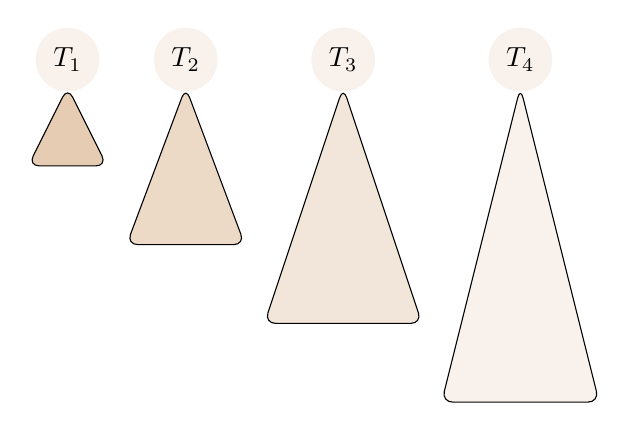
\begin{tikzpicture}
\node at (0.5cm,3.35cm) [circle,draw=brown!10,fill=brown!10] {$T_1$};
\node at (2cm,3.35cm) [circle,draw=brown!10,fill=brown!10] {$T_2$};
\node at (4cm,3.35cm) [circle,draw=brown!10,fill=brown!10] {$T_3$};
\node at (6.25cm,3.35cm) [circle,draw=brown!10,fill=brown!10] {$T_4$};
\draw[fill=brown!40,rounded corners] (0cm,2cm) -- (.5cm,3cm) -- (1cm,2cm) -- cycle;
\draw[fill=brown!30,rounded corners] (1.25cm,1cm) -- (2cm,3cm) -- (2.75cm,1cm) -- cycle;
\draw[fill=brown!20,rounded corners] (3cm,0cm) -- (4cm,3cm) -- (5cm,0cm) -- cycle;
\draw[fill=brown!10,rounded corners] (5.25cm,-1cm) -- (6.25cm,3cm) -- (7.25cm,-1cm) -- cycle;
\end{tikzpicture} 
\end{center}

\caption{An ensemble of trees of different size}
\label{fig:trees}
\end{figure}


\begin{figure}
\begin{center} 
\epsfig{file=figures/Kappa1, scale=\sizeGraph} 
\epsfig{file=figures/Kappa2, scale=\sizeGraph} 

\end{center}
\caption{Kappa-Error diagrams for ASHT bagging (left) and bagging (right) on dataset RandomRBF with drift,
plotting 90 pairs of classifiers.}

\label{fig:kappa}
\end{figure}
\BEGINOMIT
In this section, we present a new method of bagging using Hoeffding Trees of different sizes.

A {\em Hoeffding tree}~\cite{vfdt} is an incremental, anytime decision tree 
induction algorithm that is capable of learning from massive data streams, 
assuming that the distribution generating examples does not change over time.
Hoeffding trees exploit the fact that a small sample can often be enough to choose 
an optimal splitting attribute. This idea is supported mathematically by the 
Hoeffding bound, which quantifies the number of observations (in our case, 
examples) needed to estimate some statistics within a prescribed precision (in 
our case, the goodness of an attribute). 
More precisely, the Hoeffding bound states that with probability $1 - \delta$, 
the true mean of a random variable of range $R$ will not differ from the estimated 
mean after $n$ independent observations by more than:
$$ \epsilon = \sqrt{\frac{R^2 \ln(1/\delta)}{2n}}.$$
A theoretically appealing feature of Hoeffding Trees not shared by other 
incremental decision tree learners is that it has sound guarantees of performance. 
Using the Hoeffding bound one can show that its output is asymptotically nearly 
identical to that of a non-incremental learner using infinitely many examples.
See \cite{vfdt} for details. 
\ENDOMIT
\BEGINOMIT
{\em Hoeffding Window Trees}~\cite{} are decision trees 
that using Hoeffding bounds, maintain a sliding window of instances, 
and that .

\begin{itemize}
 \item place one or more change detectors at every node that will
raise a hand whenever something worth attention happens at the node
 \item create, manage, switch and delete alternate trees
 \item maintain estimators of only relevant statistics at the nodes of the current sliding window
\end{itemize}

A {\em Hoeffding Adaptive Tree} is a decision tree that evolving from Hoeffding 
Window Tree, adaptively learn from data streams that change over time
without needing a fixed size of sliding window. The optimal size of the
sliding window is a very difficult parameter to guess for users, since it depends
on the rate of change of the distribution of the dataset.
The general idea is simple: we place instances of estimators of frequency
statistics at every node, that is, replacing each
counters in the Hoeffding Window Tree with an instance of an estimator.
\ENDOMIT

In this section, we introduce the Adaptive-Size Hoeffding Tree (ASHT). It is derived
from the Hoeffding Tree algorithm with the following differences:

\begin{itemize}
\item it has a maximum number of split nodes, or {\em size}
\item after one node splits, if the number of split nodes of the ASHT tree is higher than the
maximum value, then it deletes some nodes to reduce its size
\end{itemize}

The intuition behind this method is as follows: smaller trees adapt more quickly to changes,
and larger trees do better during periods with no or little change,
simply because they were built on more data.
Trees limited to size $s$ will be reset about twice as often as
trees with a size limit of $2s$.
This creates a set of different reset-speeds for an ensemble of such trees, and
therefore a subset of trees that are a good approximation for the current rate of change. 
It is important to note that resets will happen all the time, even for stationary datasets,
but this behaviour should not have a negative impact on the ensemble's predictive performance.

When the tree size exceeds
the maximun size value, there are two different delete options:
\begin{itemize}
 \item delete the oldest node, the root, and all of its children %delete oldest node, the root node and all its children
except the one where the split has
been made. After that, the root of the
child not deleted becomes the new root
delete the oldest node, the root, and all of its children.

 %\item delete worst error node: the node with higher error and its childs
 \item delete all the nodes of the tree, i.e., restart from a new root.
\end{itemize}



We present a new bagging method that uses these Adaptive-Size Hoeffding Trees
and that sets the size for each tree (Figure~\ref{fig:trees}). 
The maximum allowed size for the $n$-th ASHT tree is
twice the maximum allowed size for the $(n-1)$-th tree. Moreover, each tree
has a weight proportional to the inverse of the square of its error, and
%The size of ASHT 
%tree $n$ is two times the size of ASHT tree $n-1$. Moreover, it uses  a weight 
%proportional to the inverse of the square of the error, and 
it monitors its error
with an exponential weighted moving average (EWMA) with $\alpha=.01$. The size of the first tree is $2$. 

With this new method, we attempt to improve bagging performance by increasing tree diversity.
It has been observed that boosting tends to produce a more diverse set of classifiers
than bagging, and this has been cited as a factor in increased performance~\cite{MargineantuD97}.

We use the Kappa statistic $\kappa$ to show how using trees of different size, we increase
the diversity of the ensemble. 
Let's consider two classifiers $h_a$ and $h_b$, a data set containing $m$ examples, and
a contingency table where cell $C_{ij}$ contains the number of examples for which $h_a(x)=i$
and $h_b(x)=j$. If $h_a$ and $h_b$ are identical on the data set, then all non-zero counts 
will appear along the diagonal. If $h_a$ and $h_b$ are very different, then there should be
a large number of counts off the diagonal. We define
$$\Theta_1= \frac{\sum^{L}_{i=1} C_{ii}}{m}$$
$$\Theta_2 = \sum^L_{i=1} \left(  \sum^L_{j=1} \frac{C_{ij}}{m} \cdot \sum^L_{j=1}\frac{C_{ji}}{m} \right) $$
We could use $\Theta_1$ as a measure of agreement, but in problems where one class is much
more common than others, all classifiers will agree by chance, so all pair of classifiers
will obtain high values for $\Theta_1$. To correct this,
the $\kappa$ statistic is defined as follows:
$$ \kappa = \frac{\Theta_1 -\Theta_2}{1-\Theta_2}$$
$\kappa$ uses $\Theta_2$, the probability that two classifiers agree by chance, given the observed counts in the table.
% The $\kappa$ statistic is defined as follows:
If two classifiers agree on every example then $\kappa = 1 $, and if their predictions
coincide purely by chance, then $\kappa = 0$.



We use the Kappa-Error diagram to compare the diversity of normal bagging with bagging using trees
of different size. The Kappa-Error diagram is a scatterplot where each point corresponds to a pair
of classifiers. The $x$ coordinate of the pair is the $\kappa$ value for the two classifiers. 
The $y$ coordinate is the average of the error rates of the two classifiers.

Figure~\ref{fig:kappa} shows the Kappa-Error diagram for the Random RBF dataset with drift parameter or
change speed equal to 0.001.% speed of change of $.001$. 
We observe that bagging classifiers are 
very similar to one another and that the decision tree classifiers of different size are very diferent from
one another.

\section{New method of Bagging using \adwin}% and Boosting}
\label{adwinbagging}
%\BEGINOMIT
\adwinb\cite{bif-gav}, as seen in Chapter~\ref{ch:adwin} is a change detector and estimator that solves in a 
well-specified way the problem of tracking the average of a stream of bits or 
real-valued numbers. \adwin keeps a variable-length window of recently seen 
items, with the property that the window has the maximal length statistically 
consistent with the hypothesis ``there has been no change in the average value
inside the window". 

%\BEGINOMIT
More precisely, an older fragment of the window is dropped if and only if 
there is enough evidence that its average value differs from that of 
the rest of the window. 
This has two consequences: one, that change reliably declared whenever
the window shrinks; and two, that at any time the average over the existing
window can be reliably taken as an estimation of the current average in the stream
(barring a very small or very recent change that is still not statistically 
visible). %A formal and quantitative statement of these two points (a theorem)
%appears in \cite{bif-gav}. 
%\ENDOMIT

\adwin is parameter- and assumption-free in the sense that 
it automatically detects and adapts to the current rate of change. 
Its only parameter is a confidence bound $\delta$,
indicating how confident we want to be in the algorithm's output, 
inherent to all algorithms dealing with random processes. 

Also important for our purposes, \adwin does not maintain the window
explicitly, but compresses it using a variant of the exponential histogram
technique in \cite{babcock-sampling}. This means that it keeps a window of length $W$
using only $O(\log W)$ memory and $O(\log W)$ processing time per item, 
rather than the $O(W)$ one expects from a na{\"\i}ve implementation. 
%\ENDOMIT

\adwin Bagging is the online bagging method % and boosting algorithms 
implemented in MOA with the  addition of the \adwin algorithm as a change 
detector and as an estimator for the weights of the boosting method.
When a change is detected, the worst classifier of the ensemble of classifiers 
is removed and a new classifier is added to the ensemble.

\section{Adaptive Hoeffding Option Trees}
\label{Ssadahot}
                                                                  
{\em Hoeffding Option Trees}~\cite{optiontrees} 
explained in Section~\ref{sec:hot} are regular Hoeffding trees 
containing additional option nodes that allow several tests to be applied, 
leading to multiple Hoeffding trees as separate paths. 
%  Hoeffding Option Trees 
They consist of a single structure that efficiently represents multiple
trees. A particular example can travel down multiple paths of the tree, contributing, 
in different ways, to different options.
% The class of a test example is
%determined by a committee made up of the predictions of all leaf nodes reached.
%In the context of a data stream, the idea is to grow multiple options in the same
%manner as a single Hoeffding tree. By doing so the effects of limited lookahead
%and instability are mitigated, leading to a more accurate model.

An {\em Adaptive Hoeffding Option Tree} is a Hoeffding Option Tree with the following improvement:
each leaf stores an estimation of the current error. It uses an EWMA
estimator with $\alpha =.2$.
The weight of each node in the voting process is 
proportional to the square of the inverse of the error.

\section{Method performance}

Bagging is clearly the best method in terms of accuracy. This superior position
is, however, achieved at high cost in terms of memory and time. 
\adwin Bagging and ASHT Bagging are the most accurate methods for most datasets, but they 
are slow.
%have a low prediction speed.
 \adwin Bagging is slower than ASHT Bagging and for some datasets it 
needs more memory. 
ASHT Bagging using weighted classifiers and replacing oversized trees 
with new ones seems to be the most accurate ASHT bagging method.
We observe that bagging using 5 trees of different size may be 
sufficient, as its error is not much {higher} %%%lower 
than for 10 trees, but it is nearly {twice as fast}. %%two times faster.
Also Hoeffding trees using drift detection methods are faster but less accurate methods.

 In~\cite{optiontrees}, a range of option limits were tested and averaged across all datasets without
concept drift to determine the optimal number of paths. This optimal number of options was five.
Dealing with concept drift, we observe that increasing the number of options to 50, 
 a significant improvement is obtained in accuracy for some datasets. 

\chapter{Restricted Hoeffding Trees Stacking}
\label{ch:stacking}
When applying boosting algorithms to build ensembles of decision trees
using a standard tree induction algorithm, the tree inducer has access
to all the attributes in the data. Thus, each tree can model
arbitrarily complex interactions between attributes in
principle. However, often the full modeling power of unrestricted
decision tree learners is not necessary to yield good accuracy with
boosting, and it may even be harmful because it can lead to
overfitting. Hence, it is common to apply boosting in conjunction with
depth-limited decision trees, where the growth of each tree is
restricted to a certain level. In this way, only a limited set of
attributes can be used in each tree, but the risk of overfitting is
reduced. In the extreme case, only a single split is allowed and the
decision trees degenerate to decision stumps. Despite the fact that
each restricted tree can only model interactions between a limited set
of attributes, the overall ensemble is often highly accurate.

The method presented in this chapter is based on this observation~\cite{BifetFHP10}. We
present an algorithm that produces a classification model based on an
ensemble of restricted decision trees, where each tree is built from a
distinct subset of the attributes. The overall model is formed by
combining the log-odds of the predicted class probabilities of these trees using sigmoid perceptrons, with one perceptron per class. In contrast to the standard boosting approach,
which forms an ensemble classifier in a greedy fashion, building each tree in
sequence and assigning corresponding weights as a by-product, our
method generates each tree in parallel and combines them using perceptron classifiers by adopting the stacking approach~\cite{stacking}. Because we
are working in a data stream scenario, Hoeffding trees~\cite{vfdt} are
used as the ensemble members. They, as well as the perceptrons,
can be trained incrementally, and we also show how \adwinb-based change
detection~\cite{bif-gav} can be used to apply the method to evolving data
streams.

There is existing work on boosting for data streams~\cite{ozabagboost}, but
the algorithm has been found to yield inferior accuracy compared to
\adwin bagging. Moreover, it is unclear how a boosting algorithm can be
adapted to data streams that evolve over time: because bagging
generates models independently, a model can be replaced when it is no
longer accurate, but the sequential nature of boosting prohibits this
simple and elegant solution. Because our method generates models
independently, we can apply this simple strategy, and we show that it yields
more accurate classifications than Online Bagging~\cite{ozabagboost} on the real-world and
artificial data streams that we consider in our experiments.

Our method is also related to work on building ensembles using random
subspace models~\cite{Random-subspace}. In the random subspace approach, each
model in an ensemble is trained based on a randomly chosen subset of
attributes. The models' predictions are then combined in an unweighted
fashion. %\footnote{Is this true?} 
Because of this latter property, the
number of attributes available to each model must necessarily be quite
large in general, so that each individual model is powerful enough to
yield accurate classifications. In contrast, in our method, we
exhaustively consider all subsets of a given, small, size, build a
tree for each subset of attributes, and then combine their predictions
using stacking. In random forests~\cite{randomforests}, the random subspace
approach is applied locally at each node of a decision tree in a
bagged ensemble. Random forests have  been applied to data streams, but did not
yield substantial improvements on bagging in this
scenario. %~\cite{leveraging}. %\footnote{Is this true?}


\section{Combining Restricted Hoeffding Trees using Stacking}

The basic method we present in this chapter is very simple: enumerate
all attribute subsets of a given user-specified size $k$, learn
a Hoeffding tree from each subset based on the incoming data stream,
gather the trees' predictions for each incoming instance, and use
these predictions to train simple perceptron classifiers. The question that needs
to be addressed is how exactly to prepare the ``meta'' level data for
the perceptrons and what shape it should take.

Rather than using discrete classifications to build the meta level
model in stacking, it is common to use class probability estimates
instead because they provide more information due to the fact that they
represent the degree of confidence that each model has in its
predictions. Hence, we also adopt this approach in our method: the
meta-level data is formed by collecting the class probability
estimates for an incoming new instance, obtained from the Hoeffding
trees built from the data observed previously.

The meta level combiner we use is based on simple perceptrons with sigmoid
activation functions, trained using stochastic gradient
descent to minimize the squared loss with respect to the actual
observed class labels in the data stream. We train one perceptron per
class value and use the Hoeffding trees' class probability estimates
for the corresponding class value to form the input data for each
perceptron.

There is one caveat. Because the sigmoid activation function is used
in the perceptrons, we do not use the raw class probability estimates
as the input values for training them. Rather, we use the log-odds of
these probability estimates instead. Let $\hat p(c_{ij}|\vec{x})$ be
the probability estimate for class $i$ and instance $\vec{x}$ obtained
from Hoeffding tree $j$ in the ensemble. Then we use
$$
a_{ij}=\log(\hat p(c_{ij}|\vec{x})/(1-\hat p(c_{ij}|\vec{x}))
$$ as the value of input attribute $j$ for the perceptron associated
with class value $i$.

Let $\vec{a_{i}}$ be the vector of log-odds for class $i$. The output
of the sigmoid perceptron for class $i$ is then
$f(\vec{a_i})=1/(1+e^{-(\vec{w_i}\vec{a_i}+b_i)})$, based on per-class
coefficients $\vec{w_i}$ and $b_i$. We use the log-odds as the inputs
for the perceptron because application of the sigmoid function
presupposes a linear relationship between $\log(f(\vec{a_i})/(1-f(\vec{a_i})))$
and $\vec{a_i}$.

To avoid the zero-frequency problem, we slightly modify the
probability estimates obtained from a Hoeffding tree by adding a small
constant $\epsilon$ to the probability for each class, and then
renormalize. In our experiments, we use $\epsilon=0.001$, but smaller
values lead to very similar results.

The perceptrons are trained using stochastic gradient descent: the
weight vector is updated each time a new training instance is obtained
from the data stream. Once the class probability estimates for that
instance have been obtained from the ensemble of Hoeffding trees, the
input data for the perceptrons can be formed, and the gradient descent
update rule can be used to perform the update. The weight values are
initialized to the reciprocal of the size of the ensemble, so that the
perceptrons give equal weight to each ensemble member initially.

A crucial aspect of stochastic gradient descent is an appropriately
chosen learning rate, which determines the magnitude of the update. If
it is chosen too large, there is a risk that the learning process will
not converge. A common strategy is to decrease it as the amount of
training data increases. Let $n$ be the number of training instances
seen so far in the data stream, and let $m$ be the number of
attributes. We set the learning rate $\alpha$ based on the following
equation: $$ \alpha=\frac{2}{2+m+n}.  $$

However, there is a problem with this approach for setting the
learning rate in the context we consider here: it assumes that the
training data is identically distributed. This is not actually the case
in our scenario because the training data for the perceptrons is
derived from the probability estimates obtained from the Hoeffding
trees, and these change over time, generally becoming more
accurate. Setting the learning rate based on the above equation means
that the perceptrons will adapt too slowly once the initial data in
the data stream has been processed.

There is a solution to this problem: the stream of predictions from
the Hoeffding trees can be viewed as an {\it evolving} data stream
(regardless of whether the underlying data stream forming the training
data for the Hoeffding trees is actually evolving) and we can use an
existing change detection method for evolving data streams to detect
when the learning rate should be reset to a larger value. We do this
very simply by setting the value of $n$ to zero when change has been
detected. To detect change, we use the \adwin change
detector~\cite{bif-gav}, which is discussed in more detail in the next
section. It detects when the accuracy of a classifier increases or
decreases significantly as a data stream is processed. We apply it to
monitor the accuracy of each Hoeffding tree in the ensemble. When
accuracy changes significantly for one of the trees, the learning
rate is reset by setting $n$ to zero. The value of $n$ is then
incremented for each new instance in the stream until a new change is
detected. This has the effect that the learning rate will be kept
relatively large while the learning curve for the Hoeffding trees has
a significant upward trend.

\subsection{\adwinb-based Change Detection}

The \adwin change detector comes with nice theoretical guarantees. In
addition to using it to reset the learning rate when necessary, we
also use it to make our ensemble classifier applicable to evolving
data stream, where the original data stream, used to train the
Hoeffding trees, changes over time.

The strategy we use to cope with evolving data streams using \adwin is
very simple: the idea is to replace ensemble members when
they start to perform poorly.  To implement this, we use \adwin to
detect when the accuracy of one of the Hoeffding trees in the ensemble
has dropped significantly.  To do this, we can use the same \adwin change
detectors that are also applied to detect when the learning rate needs
to be reset.  When one of the change detectors associated
with a particular tree reports a significant drop in accuracy, the
tree is reset and the coefficients in the perceptrons that are
associated with this tree (one per class value) are set to zero. A new
tree is then generated from new data in the data stream, so that the
ensemble can adapt to changes.

Note that all trees for which a significant drop is detected are
replaced.  Note also that a change detection event automatically
triggers a reset of the learning rate, which is important because the
perceptrons need to adapt to the changed ensemble of trees.

\subsection{A Note on Computational Complexity}

This new approach is based on generating trees for all possible attribute
subsets of size $k$. If there are $m$ attributes in total, there are
${m}\choose{k}$ of these subsets.  Clearly, only moderate values of
$k$, or values of $k$ that are very close to $m$, are feasible.  When
$k$ is one, there is no penalty with respect to computational
complexity compared to building a single Hoeffding tree, because then
there is only one tree per attribute, and an unrestricted tree also
scales linearly in the number of attributes.  If $k$ is two, there is
an extra factor of $m$ in the computational complexity compared to
building a single unrestricted Hoeffding tree, i.e. overall effort
becomes quadratic in the number of attributes.

$k=2$ is very practical even for datasets with a relatively large
number of attributes, although certainly not for very high-dimensional
data (for which linear classifiers are usually sufficient
anyway). Larger values of $k$ are only practical for small numbers of
attributes, unless $k$ is very close to $m$ (e.g. $k=m-1$). We have
used $k=4$ for datasets with 10 attributes in our experiments, with
very acceptable runtimes. It is important to keep in mind that many
practical classification problems appear to exhibit only very
low-dimensional interactions, which means small values of $k$ are
sufficient to yield high accuracy.



\chapter{Leveraging Bagging}
\label{ch:leveraging}


Bagging and Boosting are ensemble methods used to improve the accuracy of classifier methods. 
Non-streaming bagging~\cite{bagging} builds a set of  $M$ base models, training each model with a bootstrap sample of size $N$ created by drawing random samples with replacement from the original training set.  Each base model's training set contains each of the original training example $K$ times where $P(K=k)$ follows a binomial distribution. This binomial distribution  for large values of  $N$ tends to a Poisson(1) distribution, where  Poisson(1)$= \exp(-1)/k!$. Using this fact, Oza and Russell~\cite{ozabagboost,ozaexp} proposed {\em Online Bagging}, an online method that instead of sampling with replacement, gives each example a weight according to Poisson(1). 

Boosting algorithms combine multiple base models to obtain a small generalization error.
Non-streaming boosting builds a set of models sequentially, with the construction of each new model depending on the performance of the previously constructed models. The intuitive idea of boosting is to give more weight to misclassified examples, and reducing the weight of the correctly classified ones.

\BEGINOMIT
AdaBoost.M1~\cite{adaboost} generates a sequence of models using weighted training sets based on the performance of the previous model on the training set.  First, it creates a first model using the original training set, and it tests its accuracy on this training set. The weights of the correctly classified examples are scaled down, and the weights of the misclassified examples are scaled up.  The sum of the weight of the classified examples is the same as the misclassified examples. The next model is created using the learning algorithm with this new weight distribution on the training set. Doing that, some of the previously misclassified examples examples will be correctly classified by the new base model, because of their higher weights.
\ENDOMIT
%For online settings, Oza and Russell~\cite{ozabagboost,ozaexp} proposed {\em Online Boosting}, an online method that instead of building sequentially new models, each time a new instance arrive, it updates each model with a weight computed depending on the performance of the previous classifiers. 

From studies appearing in the literature~\cite{ozabagboost,ozaexp,ensemble},
Online Bagging seems to perform better than online boosting methods. Why bagging outperforms boosting in the data stream setting is still an open question. Adding more random weight to all instances seems to improve accuracy more than adding weight to misclassified instances. In this chapter %To improve the performance of bagging
 we focus on randomization as a powerful tool to increase accuracy and diversity when constructing an ensemble of classifiers.
There are three ways of using randomization:
\begin{itemize}
\item Manipulating the input data
\item Manipulating the classifier algorithms   
\item Manipulating the output targets
\end{itemize}
 
In this chapter we focus on randomizing the input data and the output prediction of online bagging.

\section{Bagging Literature}
\label{Rel}

Breiman~\cite{bagging} introduced bagging classification using the notion of an {\em order-correct} learner. An order-correct learner $\phi$ at the input $x$ is a predictor that if input $x$ results in a class more often than any other class, then $\phi$ will also predict this class at $x$ more often than any other class. An order-correct learner is not necessarily an accurate predictor but its aggregated predictor is optimal. If a predictor is good because it is order-correct for most inputs $x$ then aggregation can transform it into a nearly optimal predictor. The vital element to gain accuracy is the instability of the prediction method. A learner is unstable if a small change in the input data leads to large changes in the output.

Friedman~\cite{friedman} explained that bagging works by reducing variance without changing the bias. There are several definitions of bias and variance for classification, but the common idea is that bias measures average error over many different training sets, and variance measures the additional error due to the variation in the model produced by using different training sets.

Domingos~\cite{Domingos97} claimed that Breiman's line of reasoning is limited, since we may never know {\em a priori} whether a learner is order-correct for a given example or not, and what regions of the instance space will be order-correct or not. He explained bagging's success showing that bagging works by effectively changing a single-model learner to another single-model learner, with a different implicit prior distribution over models, one that is less biased in favor of simple models.

Some work in the literature shows that bagging asymptotically performs some smoothing on the estimate. Friedman and Hall~\cite{Friedman99onbagging} used an asymptotic truncated Taylor series of the estimate to show that in the limit of infinite samples, bagging reduces the variance of non-linear components.

B\"uhlmann and Yu~\cite{yu-bag}, analyzed bagging using also asymptotic limiting distributions, and they proposed {\em subagging} as a less expensive alternative to bagging. Subagging uses subsampling as an alternative aggregation scheme. They claimed that subagging is as accurate as bagging but uses less computation.


Grandvalet\cite{Grandvalet04} explained the performance of bagging by the goodness and badness of highly influential examples, in situations where the usual variance reduction argument is questionable. He presented an experiment showing that bagging increases the variance of decision trees, and claimed that bagging does not simply reduce variance in its averaging process.


In~Chapter~\ref{ch:ensemblemethods} two new state-of-the-art bagging methods were presented: ASHT Bagging using trees of different sizes, and \adwin Bagging using a change detector to decide when to discard underperforming 
ensemble members. 


\BEGINOMIT
\begin{algorithm}
\caption{Oza and Russell's {\em Online Bagging} for $M$ models} %in the ensemble }
\begin{algorithmic}[1]
\STATE Initialize base models $h_{m}$ for all $m \in \{1,2,...,M\}$
\FORALL{training examples}
\FOR{$m=1,2,...,M$}
\STATE Set $w = $ {\em Poisson}(1)
%\FOR{$n=1,2,...,k$}
\STATE Update $h_{m}$ with the current example with weight $w$
%\ENDFOR
\ENDFOR
\ENDFOR
\STATE {\bf anytime output:}
\RETURN hypothesis: $h_{fin}(x) = \arg \max_{y \in Y} \sum_{t=1}^{T} I(h_{t}(x) = y)$
\end{algorithmic}
\label{alg:ozabag}
\end{algorithm}
\ENDOMIT

%Boosting algorithms combine multiple base models to obtain a small generalization error.
%Non-streaming boosting builds a set of models sequentially, with the construction of each new model depending on the performance of the previous constructed models. The intuitive idea of boosting is to give more weight to the misclassified examples, and reduce the weight of the correctly classified ones.

%For online settings, Oza and Russell~\cite{ozabagboost,ozaexp} proposed {\em Online Boosting}, an online method that instead of building sequentially new models, each time a new instance arrive, it updates each model with a weight computed depending on the performance of the previous classifiers. %The pseudo-code is listed in Algorithm~\ref{alg:ozaboost}

Breiman~\cite{randomforests} proposed Random Forests as a method to use randomization on the input and on the internal construction of the decision trees. Random Forests are ensembles of trees with the following characteristics: the input training set is obtained by sampling with replacement, the nodes of the tree only may use a fixed number of random attributes to split, and the trees are grown without pruning. Abdulsalam et al.~\cite{Abdulsalam} presented a streaming version of random forests and Saffari et al.~\cite{SaffariORF2009} presented an online version.

\BEGINOMIT

\begin{algorithm}
\caption{Oza and Russell's {\em Online Boosting}.}
\begin{algorithmic}[1]
\STATE Initialize base models $h_{m}$ for all $m \in \{1,2,...,M\}, \lambda_{m}^{sc}=0, \lambda_{m}^{sw}=0$
\FORALL{training examples}
\STATE Set ``weight'' of example $\lambda_{d} = 1$
\FOR{$m=1,2,...,M$}
\STATE Set $w = $ {\em Poisson}($\lambda_{d}$)
%\FOR{$n=1,2,...,k$}
\STATE Update $h_{m}$ with the current example with weight $w$
%\ENDFOR
\IF{$h_{m}$ correctly classifies the example}
\STATE $\lambda_{m}^{sc} \gets \lambda_{m}^{sc} + \lambda_{d}$
\STATE  $\epsilon_{m} = \frac{\lambda_{m}^{sw}}{\lambda_{m}^{sc} + \lambda_{m}^{sw}}$
\STATE $\lambda_{d} \gets \lambda_{d} \left( \frac{1}{ 2( 1-\epsilon_m)} \right)$
\ELSE
\STATE $\lambda_{m}^{sw} \gets \lambda_{m}^{sw} + \lambda_{d}$
\STATE  $\epsilon_{m} = \frac{\lambda_{m}^{sw}}{\lambda_{m}^{sc} + \lambda_{m}^{sw}}$
\STATE $\lambda_{d} \gets \lambda_{d} \left( \frac{1}{2 \epsilon_m} \right)$
\ENDIF
\ENDFOR
\ENDFOR
\STATE {\bf anytime output:}
%\STATE Calculate  $\beta_{m} = \epsilon_{m} / (1 - \epsilon_{m})$ for all $m \in \{1,2,...,M\}$
\STATE Calculate  $\alpha_{m} = \log \frac{1 - \epsilon_{m}}{\epsilon_{m} } $ for all $m \in \{1,2,...,M\}$
\RETURN hypothesis: $h_{fin}(x) = \arg \max_{y \in Y} \sum_{m:h_{m}(x)=y} \alpha_{m} $
\end{algorithmic}
\label{alg:ozaboost}
\end{algorithm}

Breiman~\cite{arcing} 
proposed a simple boosting algorithm, {\em arc-x4}, to point out that the success of boosting may lay not in its specific form but in its adaptive resampling property: place increasing weight on those cases more frequently misclassified.  Arc-x4 uses an unweighted voting, and the weights used to train the models are based in the probabilities defined by

$$ p(n)= ( 1+ mc_{t}(n)^4)/ \sum(1+mc_{t}(n)^ 4)$$ 

where $mc_{t}(n)$ is the number of misclassifications of the models  $1$ to $t$ by example $n$.

The online version of {\em arc-x4} was proposed by Fern and Givan~\cite{onlinearcx4},. % and its pseudo-code is shown in Algorithm~\ref{alg:arcx4}. 
Note that they use a weighted voting strategy, but they claim that for ensemble sizes the two strategies give nearly identical results. Online arcx-4 has three steps: first it updates the vote of the model, second it computes the weight using the number of misclassification of the previous models, and finally, it trains the model with the weight calculated in the second step.



Breiman~\cite{ivotes} proposed an arcing on-line method {\em Ivotes} using the idea of importance voting. As a new example arrive, it is checked to see how it is classified by the current classifier. If misclassified it is accepted with a weight of one. If not, it is accepted with probability $e_T/(1-e_T)$, where the error estimate $e_T$ is computed as a smoothed version of the proportion of misclassified examples.
\ENDOMIT
\BEGINOMIT
\begin{algorithm}
\caption{Fern and Givan's {\em Online Arc-x4} for $M$ models} %in the ensemble }
\begin{algorithmic}[1]
\STATE Initialize base models $h_{m}$ for all $m \in \{1,2,...,M\}, v_{m} = 0$
\FORALL{training examples}

\FOR{$m=1,2,...,M$}
\IF{$h_{m}$ correctly classifies the example}
\STATE $v_{m} \gets v_{m}+1$
\ENDIF
\STATE $mc_t = 0$
\FOR{$t=1,2,...,m-1$}
\IF{$h_{t}$ correctly classifies the example}
\STATE $mc_t \gets mc_t +1$
\ENDIF
\ENDFOR
\STATE Set $w =  1 + mc_{t}^{4}$ %{\em Poisson}(1)
%\FOR{$n=1,2,...,k$}
\STATE Update $h_{m}$ with the current example with weight $w$
%\ENDFOR
\ENDFOR
\ENDFOR
\STATE {\bf anytime output:}
\RETURN hypothesis: $h_{fin}(x) = \arg \max_{y \in Y} \sum_{m:h_{m}(x)=y} v_{m}$
\end{algorithmic}
\label{alg:arcx4}
\end{algorithm}


Zhu et al.~\cite{multiclassadaboost} presented SAMME as a multi-class version of AdaBoost.M1, as AdaBoost.M1 has a strong restriction for multi-class problems: the error of each classifier has to be less than $1/2$. They presented SAMME as a method with the same simple modular structure of AdaBoost.M1, but with an important difference: the addition of the term $\log (K-1)$ to the weight $\alpha_m$ of the $m$ classifier, where $K$ is the number of classes:

$$\alpha_{m} = \log \frac{1 - \epsilon_{m}}{\epsilon_{m} } + \log (K-1)$$
 
 For two classes, the term  $\log (K-1)$ t is zero, and SAMME reduces to AdaBoost.M1. 

\ENDOMIT
\section{Leveraging Bagging}
\label{Per}

In this section, we present a new online leveraging bagging algorithm, improving Online Bagging of  Oza and Russell.
The pseudo-code of Online Bagging of Oza and Russell 
is listed in Algorithm~\ref{alg:ozabag}.

We leverage the performance of bagging, with two randomization improvements: increasing resampling and using output detection codes.


\begin{algorithm}
\caption{{\em Leveraging  Bagging} for $M$ models} %in the ensemble }
\begin{algorithmic}[1]
\STATE Initialize base models $h_{m}$ for all $m \in \{1,2,...,M\}$
\STATE Compute coloring $\mu_m(y)$
\FORALL{training examples $(x,y)$}
%\STATE $mc = 0$
%\FOR{$m=1,2,...,M$}
%\IF{$h_{m}$ correctly classifies the example}
%\STATE $mc \gets mc +1$
%\ENDIF
%\ENDFOR
\FOR{$m=1,2,...,M$}
\STATE Set $w = $ {\em Poisson}($\lambda$)
%\FOR{$n=1,2,...,k$}
\STATE Update $h_{m}$ with the current example with weight $w$ and class $\mu_m(y)$
%\ENDFOR
\ENDFOR
\ENDFOR
\IF{\adwin  detects change in error of one of the classifiers}
\STATE Replace classifier with higher error with a new one 
\ENDIF
\STATE {\bf anytime output:}
\RETURN hypothesis: $h_{fin}(x) = \arg \max_{y \in Y} \sum_{t=1}^{T} I(h_{t}(x) =\mu_t( y))$
\end{algorithmic}
\label{alg:levbag}
\end{algorithm}
 

 Resampling with replacement is done in Online Bagging using Poisson(1). 
 There are other sampling mechanisms:
 \begin{itemize}
\item    Lee and Clyde~\cite{bayesian} uses the Gamma distribution (Gamma(1,1)) to obtain a Bayesian version of Bagging. Note that Gamma(1,1) is equal to Exp(1). 
\item Bulhman and Yu~\cite{yu-bag} proposes subagging, using resampling without replacement. 
\end{itemize}

  
  \begin{figure}[h]
\begin{center} 
\epsfig{file=figures/Poisson.pdf, scale=.4}%9} 

\end{center}
\caption{Poisson Distribution.}

\label{fig:poisson}
\end{figure}
 Our proposal is to increase the weights of this resampling using a larger value $\lambda$ to compute the value of the Poisson distribution.  
The Poisson distribution is used to model the number of events occurring within a given time interval. 

Figure~\ref{fig:poisson} shows the probability function mass of the distribution of Poisson for several values of $\lambda$. The mean and variance of a Poisson distribution is $\lambda$.  
For $\lambda=1$ we see that $37\%$ of the values are zero, $37\%$ are one, and $26\%$ are values greater than one. Using a weight of Poisson(1) we are taking out   $37\%$ of the examples, and repeating $26\%$ of the examples, in a similar way to non streaming bagging.
For $\lambda=6$ we see that $0.25\%$ of the values are zero, $45\%$ are lower than six, $16\%$ are six, and $39\%$ are values greater than six.  Using a  value of $\lambda > 1$ for Poisson($\lambda$) we are increasing the diversity of the weights and modifying the input space of the classifiers inside the ensemble. However, the optimal value of $\lambda$ may be different for each dataset. 
  
 Our second improvement is to add randomization at the output of the ensemble using output codes. Dietterich and Bakiri~\cite{ecoc} introduced a method based on error-correcting output codes, which handles multiclass problems using only a binary classifier. The classes assigned to each example are modified to create a new binary classification of the data induced by a mapping from the set of classes to \{0,1\}. A variation of this method by Schapire~\cite{BoostOC} presented a form of boosting using output codes.
 
 We assign to each class a binary string of length $n$ and then build an ensemble of $n$ binary classifiers. Each of the classifiers learns one bit for each position in this binary string. When a new instance arrives, we assign $x$ to the class whose binary code is closest. We can view an error-correcting code as a form of voting in which a number of incorrect votes can be corrected.
 
We use random output codes instead of deterministic codes. In standard ensemble methods, all classifiers try to predict the same function. However, using output codes each classifier will predict a different function. This may reduce the effects of correlations between the classifiers, and increase diversity of the ensemble.

We implement random output codes in the following way: we choose for each classifier $m$ and class $c$ a binary value $\mu_m(c)$ in a uniform, independent, and random way. We ensure that exactly half of the classes are mapped to $0$. The output of the classifier for an example is the class which has more votes of its binary mapping classes. Table~\ref{tab:codes} shows an example for an ensemble of 6 classifiers in a classification task of 3 classes. 
 
 \begin{table}[h]
\caption{Example matrix of random output codes for 3 classes and 6 classifiers}
 \begin{center}
  \begin{tabular}{| l | c | c | c | }
    \hline
     &  Class 1 & Class 2 & Class 3  \\ \hline
   Classifier 1 & 0 & 0 & 1  \\ 
   Classifier 2 & 0 & 1 & 1  \\ 
   Classifier 3 & 1 & 0 & 0  \\
   Classifier 4 & 1 & 1 & 0  \\
   Classifier 5 & 1 & 0 & 1  \\
   Classifier 6 & 0 & 1 & 0  \\
    \hline
  \end{tabular}
\end{center}
\label{tab:codes}
\end{table}%

 
We use the same strategy as in Chapter~\ref{ch:ensemblemethods}.
\adwinb~\cite{bif-gav} is a change detector and estimator that solves in a 
well-specified way the problem of tracking the average of a stream of bits or 
real-valued numbers. \adwin keeps a variable-length window of recently seen 
items, with the property that the window has the maximal length statistically 
consistent with the hypothesis ``there has been no change in the average value
inside the window". 

\BEGINOMIT
More precisely, an older fragment of the window is dropped if and only if 
there is enough evidence that its average value differs from that of 
the rest of the window. 
This has two consequences: one, that change reliably declared whenever
the window shrinks; and two, that at any time the average over the existing
window can be reliably taken as an estimation of the current average in the stream
(barring a very small or very recent change that is still not statistically 
visible). A formal and quantitative statement of these two points (a theorem)
appears in \cite{bif-gav}. 
\ENDOMIT

\adwin is parameter- and assumption-free in the sense that 
it automatically detects and adapts to the current rate of change. 
Its only parameter is a confidence bound $\delta$,
indicating how confident we want to be in the algorithm's output, 
inherent to all algorithms dealing with random processes. 

Also important for our purposes, \adwin does not maintain the window
explicitly, but compresses it using a variant of the exponential histogram
technique. % in \cite{babcock-sampling}. 
This means that it keeps a window of length $W$
using only $O(\log W)$ memory and $O(\log W)$ processing time per item. %, 


Algorithm~\ref{alg:levbag} shows the pseudo-code of our Leveraging Bagging.
First we build a matrix with the values of $\mu$ for each classifier and class. 
For each new instance that arrives,  we give it a random weight of $Poisson(k)$.
We train the classifier with this weight,
and when a change is detected, the worst classifier of the ensemble of classifiers 
is removed and a new classifier is added to the ensemble.
To predict the class of an example, we compute for each class $c$ the sum of the votes for $\mu(c)$ of all the ensemble classifiers, and we output as a prediction the class with the most votes.



\chapter{Twitter Stream Mining}
\label{ch:twitter}
\renewcommand{\v}[1]{\ensuremath{\mathbf{#1}}}
Twitter is a ``what's-happening-right-now'' tool that enables interested
parties to follow individual users' thoughts and commentary on events
in their lives---in almost real-time~\cite{tech-crunch}. It is a potentially valuable
source of data that can be used to delve into the thoughts of millions
of people as they are uttering them.  Twitter makes these utterances
immediately available in a data stream, which can be mined using
appropriate stream mining techniques.  In principle, this could make
it possible to infer people's opinions, both at an individual level as
well as in aggregate, regarding potentially any subject or event~\cite{tech-crunch}.

%Traditional web search engines are useful because they capture
%people's intent, what they are looking for, what they desire, and what
%they want to learn about. Instead, Twitter data streams help to
%capture what people are doing and what they are thinking about.

At the official Twitter Chirp developer conference in April 2010~\cite{business-insider}, the
company presented some statistics about its site and its users.  In
April 2010, Twitter had 106 million registered users, and 180 million
unique visitors every month. New users were signing up at a rate of
300,000 per day.  Twitter's search engine received around 600 million
search queries per day, and Twitter received a total of 3 billion
requests a day via its API. Of Twitter's active users, 37 percent used
their phone to tweet.

Twitter data follows the data stream model. In this model, data arrive
at high speed, and algorithms that process them must be able to predict
in real time and do so under very
strict constraints of space and time.  Data streams pose several
challenges for algorithm design. First, they must make use
of limited resources (time and memory).  Second, they must deal with
data whose nature or distribution changes over time.

The main Twitter data stream that provides all messages from every
user in real-time is called Firehose~\cite{streaming-api} and was made available to
developers in 2010. To deal with this large amount of data,
and to use it for sentiment analysis and opinion mining---the task
considered in this chapter---streaming techniques are needed. However,
to the best of our knowledge, data stream algorithms, in conjunction
with appropriate evaluation techniques, have so far not been
considered for this task.

Evaluating data streams in real time is a challenging task.
Most work in the literature considers only how to build a picture of accuracy over time. Two main
approaches arise~\cite{MOA}:
\begin{itemize}
 \item {\bf Holdout}: Performance is measured using on single hold-out set.
\item {\bf Interleaved Test-Then-Train or Prequential}:
 Each individual example is used to test the model
before it is used for training, and accuracy is incrementally
updated. 
\end{itemize}
  
A common problem is that for unbalanced data streams with, for example, 90\% of the instances in
one class, the simplest classifiers will have high accuracies of at least 90\%. To deal with
this type of data stream,
we propose the Kappa statistic, based on a sliding window, as a measure for classifier performance
in unbalanced class streams~\cite{BifetF10}.

\section{Mining Twitter Data: Challenges}
\label{sec:challenges}

Twitter has its own conventions that renders it distinct from other
textual data. Consider the following Twitter example message
(``tweet''): \texttt{RT @toni has a cool \#job}. It shows that users
may reply to other users by indicating user names using the character
@, as in, for example, \texttt{@toni}.  Hashtags (\#) are used to
denote subjects or categories, as in, for example \texttt{\#job}.
\texttt{RT} is used at the beginning of the tweet to indicate that the
message is a so-called ``retweet'', a repetition or reposting of a
previous tweet.

In the knowledge discovery context, there are two fundamental data
mining tasks that can be considered in conjunction with Twitter data:
(a) graph mining based on analysis of the links amongst messages, and
(b) text mining based on analysis of the messages' actual text.

Twitter graph mining has been used to tackle several interesting problems:
\begin{itemize}
 \item \textbf{Measuring user influence and dynamics of
   popularity}. Direct links indicate the flow of information, and
   thus a user's influence on others. There are three measures of
   influence: indegree, retweets and mentions. Cha et
   al.~\cite{icwsm10cha} show that popular users who have high
   indegree are not necessarily influential in terms of retweets or
   mentions, and that influence is gained through concerted effort
   such as limiting tweets to a single topic.
  \item \textbf{Community discovery and formation}. Java et
    al.~\cite{java} found communities using HyperText Induced Topic
    Search (HITS)~\cite{HITS}, and the Clique Percolation
    Method~\cite{CPM}.  Romero and Kleinberg~\cite{romero} analyze
    the formation of links in Twitter via the directed closure
    process.
%  \item Information-seeking and collective problem-solving 
  \item \textbf{Social information diffusion}. De Choudhury et
    al.~\cite{choudhury:sampling} study how data sampling strategies
    impact the discovery of information diffusion.
\end{itemize}

There are also a number of interesting tasks that have been tackled
using Twitter text mining: sentiment analysis, which is the
application we consider in this chapter, classification of tweets
into categories, clustering of tweets and trending topic detection.

Considering sentiment analysis~\cite{Liu:06a,Pang+Lee:08b}, O'Connor et al.~\cite{Oconnor10} found
that surveys of consumer confidence and political opinion correlate
with sentiment word frequencies in tweets, and propose text stream
mining as a substitute for traditional polling.  Jansen et
al.~\cite{Jansen} discuss the implications for organizations of using
micro-blogging as part of their marketing strategy.  Pak et
al.~\cite{PAK} used classification based on the multinomial na\"{\i}ve
Bayes classifier for sentiment analysis. Go et al.~\cite{gohuang}
compared multinomial na\"{\i}ve Bayes, a maximum entropy classifier,
and a linear support vector machine; they all exhibited broadly
comparable accuracy on their test data, but small differences could be
observed depending on the features used.


\subsection{The Twitter Streaming API} 
\label{sec:api}

The Twitter Application Programming Interface (API)~\cite{api}
currently provides a Streaming API and two discrete REST APIs. The
Streaming API~\cite{streaming-api} provides real-time access to Tweets
in sampled and filtered form. The API is HTTP based, and GET, POST,
and DELETE requests can be used to access the data.

In Twitter terminology, individual messages describe the ``status'' of
a user. The streaming API allows near real-time access to subsets of
public status descriptions, including replies and mentions created by
public accounts.  Status descriptions created by protected accounts
and all direct messages are not available.  An interesting property of
the streaming API is that it can filter status descriptions using
quality metrics, which are influenced by frequent and repetitious
status updates, etc.

The API uses basic HTTP authentication and requires a valid Twitter
account.  Data can be retrieved as XML and the more succinct JSON
format. Parsing JSON data from the streaming API is simple: every
object is returned on its own line, and ends with a carriage return.
%Figure~\ref{fig:tweet} shows a JSON
%tweet retrieved using the Twitter Streaming API.

%The statuses/sample feed is sampled from the stream of public statuses. No
%additional data can be gleaned by consuming more than one sampled feed at a
%given access level or additional feeds at a lower access levels. All feeds at a
%given access level are identical, and all lower access levels are strict subsets
%of higher access levels. Long-term consumption of duplicate data wastes limited
%resources and may lead to a ban from the service.
\BEGINOMIT
The main Twitter stream, which provides all status updates from
everyone in real-time, is called Firehose~\cite{streaming-api}. Two subsamples of this
stream are defined as the so-called ``Spritzer'' role and
``Gardenhose'' role respectively. The sampling rate is 5\% for the
Spritzer role and 15\% for Gardenhose. 
\ENDOMIT
%The exact sampling procedure is
%as follows: The status id modulo 100 is taken on each public status,
%that is, from the Firehose. Modulus values from 0-4 are delivered to
%Spritzer, and values 0-14 are delivered to Gardenhose.
%Over a significant period, a 5\% and a 15\% sample of public statuses is
%approached. 

\BEGINOMIT
\begin{figure}

\begin{verbatim}
 {
  :favorited=>false, 
  :source=>"web", 
  :created_at=>"Wed Sep 23 18:12:25 +0000 2009", 
  :text=>"Voor de marketeers: Jan Bunt op Molblog over de gevolgen van het
aandeelhouders- model voor het marketingdenken: http://tinyurl.com/nps6tg", 
  :user=>{
    :profile_background_color=>"9ae4e8", 
    :description=>"marketeer, sportief, ondernemer", 
    :location=>"", 
    :profile_sidebar_border_color=>"87bc44", 
    :profile_link_color=>"0000ff", 
    :created_at=>"Sun Jul 05 08:45:41 +0000 2009", 
    :screen_name=>"nicknijhuis", 
   
:profile_background_image_url=>"http://s.twimg.com/a/1253301564/images/themes/th
eme1/bg.png", 
    :profile_background_tile=>false, 
    :protected=>false, 
    :url=>"http://www.linkedin.com/in/nicknijhuis", 
    :time_zone=>"Amsterdam", 
    :profile_text_color=>"000000", 
    :friends_count=>9, 
   
:profile_image_url=>"http://a1.twimg.com/profile_images/342659888/portret_nick_k
lein_normal.jpg", 
    :statuses_count=>29, 
    :utc_offset=>3600, 
    :name=>"Nick Nijhuis", 
    :following=>nil, 
    :profile_sidebar_fill_color=>"e0ff92", 
    :id=>53871280, 
    :favourites_count=>0, 
    :verified=>false
  }, 
  :truncated=>false, 
  :in_reply_to_user_id=>nil, 
  :id=>4321391704, 
  :in_reply_to_status_id=>nil, 
  :in_reply_to_screen_name=>nil
}

\end{verbatim} 

\begin{verbatim}
{
  "in_reply_to_user_id":21611055,
  "text":"@LisaDuncan66 Nice looking background! :) Good job!!",
  "geo":null,
  "coordinates":null,
  "source":"web",
  "created_at":"Tue May 11 05:25:52 +0000 2010",
  "in_reply_to_screen_name":"LisaDuncan66",
  "favorited":false,
  "truncated":false,
  "in_reply_to_status_id":13770498708,
  "place":null,
  "user" {
    "friends_count":349,
    "profile_text_color":"f320ca",
    "profile_image_url":"http://a3.twimg.com/.../Moi02_normal.jpg",
    "geo_enabled":false,
    "notifications":null,
    "favourites_count":4,
    "profile_link_color":"004cff",
    "screen_name":"VDanielleM",
    "description":"Press attach\u00e9/assistant and aspiring author",
    "time_zone":"Eastern Time (US & Canada)",
    "created_at":"Thu Jul 24 23:21:05 +0000 2008",
    "profile_sidebar_fill_color":"0a0b0b",
    "statuses_count":1573,
    "lang":"en",
    "profile_background_image_url":"http://a1.twimg.com/.../MilkyWayRoad_landolfi.jpg",
    "profile_sidebar_border_color":"050505",
    "location":"Montreal, Canada",
    "contributors_enabled":false,
    "following":null,
    "protected":false,
    "profile_background_tile":true,
    "name":"Danielle Miron",
    "profile_background_color":"111313",
    "followers_count":199,
    "id":15590776,
    "verified":false,
    "utc_offset":-18000,
    "url":"http://www.facebook.com/people/Danielle-Miron/727215550"
    },
  "id":13771698155,
  "contributors":null
} 
\end{verbatim}

\caption{Example of tweet retrieved using the Twitter Streaming API}
\label{fig:tweet}
\end{figure} 
\ENDOMIT 
\section{Twitter Sentiment Analysis}
\label{sec:sentiment}

Sentiment analysis can be cast as a classification problem where the
task is to classify messages into two categories depending on whether
they convey positive or negative feelings.% See~\cite{Pang+Lee:08b} for
%a survey of sentiment analysis, and \cite{Liu:06a} for opinion mining
%techniques.

Twitter sentiment analysis is not an easy task because a tweet can
contain a significant amount of information in very compressed form, and
simultaneously carry positive and negative feelings. Consider the
following example:
\begin{quote}
\texttt{I currently use the Nikon D90 and love it, but not as much as the Canon
40D/50D. I chose the D90 for the  video feature. My mistake.}
\end{quote} 
Also, some tweets may contain sarcasm or irony~\cite{carvalho} as in the following example:
\begin{quote}
\texttt{After a whole 5 hours away from work, I get to go back again, I'm so
lucky! }
\end{quote}
%\begin{quote}
%\texttt{``Losing followers is always cool....yaknow. ''}
%\end{quote} 
To build classifiers for sentiment analysis, we need to collect
training data so that we can apply appropriate learning algorithms.
Labeling tweets manually as positive or negative is a laborious and
expensive, if not impossible, task.  However, a significant advantage
of Twitter data is that many tweets have author-provided sentiment
indicators: changing sentiment is implicit in the use of various types
of emoticons. Hence we may use these to label our training data.  

{\em Smileys} or {\em emoticons} are visual cues that are associated
with emotional states~\cite{Read:05a,carvalho}.  They are constructed using the
characters available on a standard keyboard, representing a facial
expression of emotion. %Table~\ref{tab:emoticons} shows some examples.
When the author of a tweet uses an emoticon, they are annotating their
own text with an emotional state. Annotated tweets can be used to
train a sentiment classifier.

\section{Streaming Data Evaluation with Unbalanced Classes} 
%Kappa Statistic for Streaming Data}
\label{sec:kappa}

In data stream mining, the most frequently used measure for evaluating
predictive accuracy of a classifier is prequential
accuracy~\cite{GamaSR09}. We argue that this measure is only
appropriate when all classes are balanced, and have (approximately)
the same number of examples.  In this section, we propose the Kappa
statistic as a more sensitive measure for quantifying the predictive
performance of streaming classifiers. For example, considering the
particular target domain in this chapter, the rate in which the Twitter
Streaming API delivers positive or negative tweets may vary over time;
we cannot expect it to be 50\% all the time. Hence, a measure that
automatically compensates for changes in the class distribution should
be preferable.

Just like accuracy, Kappa needs to be estimated using some sampling
procedure. Standard estimation procedures for small datasets, such as
cross-validation, do not apply. In the case of very large datasets or
data streams, there are two basic evaluation procedures: holdout
evaluation and prequential evaluation. Only the latter provides a
picture of performance over time. In prequential evaluation (also
known as interleaved test-then-train evaluation), each example in a
data stream is used for testing before it is used for training.

We argue that prequential accuracy is not well-suited for data streams
with unbalanced data, and that a prequential estimate of Kappa should
be used instead.
Let $p_0$ be the
classifier's prequential accuracy, and $p_c$ the probability that a
chance classifier---one that assigns the same number of examples to
each class as the classifier under consideration---makes a correct
prediction.
 Consider the simple confusion matrix shown in
Table~\ref{tab:kappa}.  From this table, we see that Class+ is
predicted correctly 75 out of 100 times, and Class- is predicted
correctly 10 times. So accuracy $p_0$ is $85\%$. However a classifier
predicting solely by chance---in the given proportions---will predict
Class+ and Class- correctly in 68.06\% and 3.06\% of cases
respectively. Hence, it will have an accuracy $p_c$ of 71.12\% as
shown in Table~\ref{tab:kappa2}.

Comparing the classifier's observed accuracy to that of a chance
predictor renders its performance far less impressive than it first
seems. The problem is that one class is much more frequent than the
other in this example and plain accuracy does not compensate for
this. The Kappa statistic, which normalizes a classifier's accuracy by
that of a chance predictor, is more appropriate in scenarios such as
this one.

%A classifier that uses the majority class to predict has an accuracy on the
%confusion matrix in Table~\ref{tab:kappa} of 83\%. So, the prequential accuracy
%of $85\%$ of this classifier is not a good indicator of how well the classifier
%is performing. We need another measure to report accuracy.%, and we propose to
%use the Kappa Statistic.

\begin{table}[t]
 \begin{center} 
\begin{tabular}{lccc} \cline{2-4}
& Predicted & Predicted & \\
&  Class+&  Class-&Total\\ \hline
Correct Class+ &75&	8&	83 \\
Correct Class-&7&	10&	17 \\ \hline
Total &82&	18&	100 \\
\end{tabular}
\end{center}
\caption{Simple confusion matrix example}
\label{tab:kappa}
\end{table} 

\begin{table}[t]
 \begin{center} 
\begin{tabular}{lccc} \cline{2-4}
& Predicted & Predicted & \\
&  Class+&  Class-&Total\\ \hline
Correct Class+ &68.06&	14.94&	83 \\
Correct Class-&13.94&	3.06&	17\\ \hline
Total &82&	18&	100 \\
\end{tabular}
\end{center}
\caption{Confusion matrix for chance predictor based on example in
Table~\ref{tab:kappa}}
\label{tab:kappa2}
\end{table} 

The Kappa statistic $\kappa$ was introduced by Cohen~\cite{cohen}.  We
argue that it is particularly appropriate in data stream mining due to
potential changes in the class distribution.  Consider a classifier
$h$, a data set containing $m$ examples and $L$ classes, and a contingency table where
cell $C_{ij}$ contains the number of examples for which $h(x)=i$ and
the class is $j$.  If $h(x)$ correctly predicts all the data, then all
non-zero counts will appear along the diagonal. If $h$ misclassifies
some examples, then some off-diagonal elements will be non-zero.

We define
$$p_0= \frac{\sum^{L}_{i=1} C_{ii}}{m}$$
$$p_c = \sum^L_{i=1} \left( \sum^L_{j=1} \frac{C_{ij}}{m} \cdot
\sum^L_{j=1}\frac{C_{ji}}{m} \right) $$ 

In problems where one class is much more common than the others, any
classifier can easily yield a correct prediction by chance, and it
will hence obtain a high value for $p_0$.  To correct for this, the
$\kappa$ statistic is defined as follows:
$$ \kappa = \frac{p_0 -p_c}{1-p_c}$$
%$\kappa$ uses $p_c$, the probability that the classifiers predicts correctly by
%chance, given the observed counts in the table.
If the classifier is always correct then $\kappa = 1 $. If its
predictions coincide with the correct ones as often as those of the
chance classifier, then $\kappa = 0$.

The question remains as to how exactly to compute the relevant counts
for the contingency table: using all examples seen so far is not
useful in time-changing data streams.  Gama et al.~\cite{GamaSR09}
propose to use a forgetting mechanism for estimating prequential
accuracy: a sliding window of size $w$ with the most recent
observations, or fading factors that weigh observations using a decay
factor $\alpha$. As the output of the two mechanisms is very
similar (every window of size $w_0$ may be approximated by some decay
factor $\alpha_0$), we propose to use the Kappa statistic measured
using a sliding window. Note that, to calculate the statistic for an
$n_c$ class problem, we need to maintain only $2 n_c + 1$
estimators. We store the sum of all rows and columns in the confusion
matrix ($2 n_c$ values) to compute $p_c$, and we store the prequential
accuracy $p_0$. The ability to calculate it efficiently is an
important reason why the Kappa statistic is more appropriate for data
streams than a measure such as the area under the ROC curve.



\section{Data Stream Mining Methods}
\label{sec:methods}
%\subsection{Data Stream Mining Methods}

There are  three fast incremental methods that are well-suited
to deal with text data streams: multinomial na\"{\i}ve Bayes, stochastic
gradient descent, and the Hoeffding tree.

\subsubsection{Multinomial Na\"{\i}ve Bayes}

The multinomial na\"{\i}ve Bayes classifier is a popular classifier
for document classification that often yields %surprisingly 
good performance. It can be trivially applied to data streams because it is
straightforward to update the counts required to estimate conditional
probabilities.. 

Multinomial naive Bayes considers a document as a bag-of-words. For
each class $c$, $P (w|c)$, the probability of observing word $w$ given
this class, is estimated from the training data, simply by computing
the relative frequency of each word in the collection of training
documents of that class. The classifier also requires the prior
probability $P (c)$, which is straightforward to estimate. 

Assuming $n_{wd}$ is the number of times word $w$ occurs in document
$d$, the probability of class $c$ given a test document is calculated
as follows:
$$P(c|d) =\frac{P(c) \prod_{w\in d} P(w|c)^{n_{wd}}}{P(d)},$$
where $P (d)$ is a normalization factor. To avoid the zero-frequency
problem, it is common to use the Laplace correction for all
conditional probabilities involved, which means all counts are
initialized to value one instead of zero.

\subsubsection{Stochastic Gradient Descent}

Stochastic gradient descent (SGD) has experienced a revival since it
has been discovered that it provides an efficient means to learn
some classifiers even if they are based on non-differentiable loss
functions, such as the hinge loss used in support vector machines. In
our experiments we use an implementation of vanilla stochastic
gradient descent with a fixed learning rate, optimizing the hinge loss
with an $L_2$ penalty that is commonly applied to learn support vector
machines. With a linear machine, which is frequently applied for document
classification, the loss function we optimize is:
$$\frac{\lambda}{2} ||\v{w}||^2 + \sum{[1 - ( y \v{x} \v{w} +
  b )]_+},$$ where $w$ is the weight vector, $b$ the bias, $\lambda$ the
regularization parameter, and the class labels $y$ are assumed to be
in $\{+1,-1\}$.

We compared the performance of our vanilla implementation to that of
the Pegasos method~\cite{pegasos}, which does not require
specification of an explicit learning rate, but did not observe a gain
in performance using the latter. On the contrary, the ability to
specify an explicit learning rate turned out to be crucial to deal
with time-changing Twitter data streams : setting the learning rate to
a value that was too small meant the classifier adapted too slowly to
local changes in the distribution. In our experiments, we used
$\lambda=0.0001$ and set the learning rate for the per-example updates
to the classifier's parameters to 0.1.


%--- Bibliography -------------------
%\addcontentsline{toc}{chapter}{\bibname}
\cleardoublepage

%\bibliography{thesis}

%\bibliographystyle{alpha}%plain}
\phantomsection % Ensures that a PDF bookmark is set here
\addcontentsline{toc}{part}{Bibliography}
\bibliographystyle{plain}
\bibliography{StreamMining}

\end{document}